%
% Copyright 2018 Joel Feldman, Andrew Rechnitzer and Elyse Yeager.
% This work is licensed under a Creative Commons Attribution-NonCommercial-ShareAlike 4.0 International License.
% https://creativecommons.org/licenses/by-nc-sa/4.0/
%
\documentclass[12pt,letterpaper]{book}

\usepackage{parskip}

\usepackage{clp_notes_header}
\graphicspath{{./figures/}}
\usepackage{qhas}

\usepackage{xr}
\externaldocument{../textbook/clp_1_dc_text}


%%%%%%%%%%%%%%%%%%%%%%%%%%%%%%%%%
%%%%%%%%%%%%%%%%%%%%%%%%%%%%%%%%%

\begin{document}

\begin{titlepage}
\begin{center}
\textsc{\LARGE
CLP-I Differential Calculus\\[2ex]
Questions
}\\[2ex]

\vspace{5ex}
\hrule
\vspace{5ex}

\begin{tabular}{lcccr}
&& \large Elyse \textsc{Yeager} \\[3ex]
 Joel \textsc{Feldman}
&\quad & &\quad&
Andrew \textsc{Rechnitzer}
\end{tabular}

\end{center}
\vspace{2ex}
\hrule

\vfill
\textsc{This document was typeset on \today.}
\end{titlepage}

\subsection*{Legal stuff}
\begin{itemize}
 \item Copyright \copyright\ 2016, 2017, 2018 Joel Feldman, Andrew Rechnitzer and Elyse Yeager.

\item This work is licensed under the
Creative Commons Attribution-NonCommercial-ShareAlike 4.0 International
License. You can view a copy of the license at \\
\url{http://creativecommons.org/licenses/by-nc-sa/4.0/}.
\begin{center}
 
\includegraphics{by-nc-sa.pdf}
\end{center}


\item Links to the source files can be found at the \href{http://www.math.ubc.ca/~CLP/index.html}{text webpage}
\end{itemize}


\frontmatter

\chapter{How to use this book}
\section*{Introduction}
First of all, welcome to Calculus!

This book is written as a companion to the \href{http://www.math.ubc.ca/~andrewr/maths100180/2016/CLP/clp_notes_100.pdf}{CLP notes}.

\subsection*{How to Work Questions}

This book is organized into four sections: Questions, Hints, Answers, and Solutions. As you are working problems, resist the temptation to prematurely peek at the back! It's important to allow yourself to struggle for a time with the material. Even professional mathematicians don't always know right away how to solve a problem. The art is in gathering your thoughts and figuring out a strategy to use what you know to find out what you don't.

If you find yourself at a real impasse, go ahead and look for a hint in the Hints section. Think about it for a while, and don't be afraid to read back in the notes to look for a key idea that will help you proceed. If you still can't solve the problem, well, we included the Solutions section for a reason! As you're reading the solutions, try hard to understand why we took the steps we did, instead of memorizing step-by-step how to solve that one particular problem.

If you struggled with a question quite a lot, it's probably a good idea to return to it in a few days. That might have been enough time for you to internalize the necessary ideas, and you might find it easily conquerable. Pat yourself on the back--sometimes math makes you feel good! If you're still having troubles, read over the solution again, with an emphasis on understanding why each step makes sense.

One of the reasons so many students are required to study calculus is the hope that it will improve their problem-solving skills. In this class, you will learn lots of concepts, and be asked to apply them in a variety of situations. Often, this will involve answering one really big problem by breaking it up into manageable chunks, solving those chunks, then putting the pieces back together. When you see a particularly long question, remain calm and look for a way to break it into pieces you can handle.

\subsection*{Working with Friends}

Study buddies are fantastic! If you don't already have friends in your class, you can ask your neighbours in lecture to form a group. Often, a question that you might bang your head against for an hour can be easily cleared up by a friend who sees what you've missed. Regular study times make sure you don't procrastinate too much, and friends help you maintain a positive attitude when you might otherwise succumb to frustration. Struggle in mathematics is desirable, but suffering is not.

When working in a group, make sure you try out problems on your own before coming together to discuss with others. Learning is a process, and getting answers to questions that you haven't considered on your own can rob you of the practice you need to master skills and concepts, and the tenacity you need to develop to become a competent problem-solver.

\subsection*{Types of Questions}
\begin{Mquestion}%make this an Mquestion to be cute
Questions outlined in blue make up the \emph{representative question set}. This set of questions is intended to cover the most essential ideas in each section. These questions are usually highly typical of what you'd see on an exam, although some of them are atypical but carry an important moral. If you find yourself unconfident with the idea behind one of these, it's probably a good idea to practice similar questions.

This representative question set is our suggestion for a minimal selection of questions to work on.  You are highly encouraged to work on more.
\end{Mquestion}

\begin{question}[year]
In addition to original problems, this book contains problems pulled from quizzes and exams given at UBC for Math 100 and 180 (first-semester calculus) and Math 120 (honours first-semester calculus). These problems are marked with a star. The authors would like to acknowledge the contributions of the many people who collaborated to produce these exams over the years.
\end{question}

\Instructions{Instructions and other comments that are attached to more than one question are written in this font. The questions are organized into \Conceptual, \Procedural, and \Application.} 

\subsection*{\Conceptual}The first category is meant to test and improve your understanding of basic underlying concepts. These often do not involve much calculation. They range in difficulty from very basic reviews of definitions to questions that require you to be thoughtful about the concepts covered in the section.

\subsection*{\Procedural} Questions in this category are for practicing skills. It's not enough to understand the philosophical grounding of an idea: you have to be able to apply it in appropriate situations. This takes practice!

\subsection*{\Application} The last questions in each section go a little farther than \Procedural. Often they will combine more than one idea, incorporate review material, or ask you to apply your understanding of a concept to a new situation.

In exams, as in life, you will encounter questions of varying difficulty. A good skill to practice is recognizing the level of difficulty a problem poses. Exams will have some easy questions, some standard questions, and some harder questions.

% \subsection*{Acknowledgements}
% The authors of this text are affiliated with the University of British Columbia. The campus on Point Grey where we work sits on the traditional territory of the \href{http://www.musqueam.bc.ca}{Musqueam First Nation}. UBC and Musqueam have an ongoing relationship, formalized by a Memorandum of Affiliation, encouraging the groups to share their relative strengths for the benefit of all. More information can be found at  \url{http://aboriginal.ubc.ca/community-youth/musqueam-and-ubc/}.
% 
% Elyse would like to thank her husband Se\c{c}kin Demirba\c{s} for his endless patience, tireless support, and insightful feedback.
% 
% Joel and Andrew would like to thank some people, too.


\addtocontents{toc}{\protect\hypertarget{toc}{}}
\tableofcontents

\mainmatter


\part{The questions}

%%%%%%%%%%%%%%%%%%%%%
\chapter{Limits}
\section{Drawing Tangents and a First Limit}
%
% Copyright 2018 Joel Feldman, Andrew Rechnitzer and Elyse Yeager.
% This work is licensed under a Creative Commons Attribution-NonCommercial-ShareAlike 4.0 International License.
% https://creativecommons.org/licenses/by-nc-sa/4.0/
%
\questionheader{ex:s1.1}

%%%%%%%%%%%%%%%%%%
\subsection*{\Conceptual}
%%%%%%%%%%%%%%%%%%
\begin{Mquestion}
On the graph below, draw:
\begin{enumerate}[(a)]
\item\label{s1.1p1.1} The tangent line to $y=f(x)$ at $P$,
\item\label{s1.1p1.2}  the tangent line to $y=f(x)$ at $Q$, and
\item\label{s1.1p1.3}  the secant line to $y=f(x)$ through $P$ and $Q$.
\end{enumerate}
\begin{center}
\begin{tikzpicture}
\YEaaxis{1}{5}{1}{3}
\draw[thick] plot[domain=-1:5, samples=100](\x,{(3*\x-10)*(\x+1)*(\x-2)/30}) node[right]{$y=f(x)$};
\draw (1,7/15) node[vertex, label=above:$P$]{};
\draw (4.5,7*11/48) node[vertex, label= left:$Q$]{};
\end{tikzpicture}
\end{center}
\end{Mquestion}
\begin{answer}
\begin{center}
\begin{tikzpicture}
\YEaaxis{1}{5}{1}{3}
\draw[thick] plot[domain=-1:5, samples=100](\x,{(3*\x-10)*(\x+1)*(\x-2)/30}) node[right]{$y=f(x)$};
\draw (1,7/15) node[vertex, label=above:$P$]{};
\draw (4.5,7*11/48) node[vertex, label= left:$Q$]{};
\draw[thick, blue] plot[domain=-1:3.5] (\x,{27/30-13/30*\x}) node[below left]{\ref{s1.1p1.1}};
\draw[thick, green] plot[domain=3.5:5.5] (\x,{7*11/48+2.31*(\x-4.5)}) node[left]{\ref{s1.1p1.2}};
\draw[thick, red] plot[domain=0:5.5] (\x,{7/15+.325*(\x-1)}) node[right]{\ref{s1.1p1.3}};
\end{tikzpicture}
\end{center}
\end{answer}
\begin{solution}
\begin{center}
\begin{tikzpicture}
\YEaaxis{1}{5}{1}{3}
\draw[thick] plot[domain=-1:5, samples=100](\x,{(3*\x-10)*(\x+1)*(\x-2)/30}) node[right]{$y=f(x)$};
\draw (1,7/15) node[vertex, label=above:$P$]{};
\draw (4.5,7*11/48) node[vertex, label= left:$Q$]{};
\draw[thick, blue] plot[domain=-1:3.5] (\x,{27/30-13/30*\x}) node[below left]{\ref{s1.1p1.1}};
\draw[thick, green] plot[domain=3.5:5.5] (\x,{7*11/48+2.31*(\x-4.5)}) node[left]{\ref{s1.1p1.2}};
\draw[thick, red] plot[domain=0:5.5] (\x,{7/15+.325*(\x-1)}) node[right]{\ref{s1.1p1.3}};
\end{tikzpicture}
\end{center}
The tangent line to $y=f(x)$ at a point should go through
  the point, and be ``in the same direction" as $f$ at that point. The secant line through $P$ and $Q$ is simply the straight line passing through $P$ and $Q$.
\end{solution}

%
\begin{Mquestion}
Suppose a curve $y=f(x)$ has tangent line $y=2x+3$ at the point $x=2$.
\begin{enumerate}[(a)]
\item True or False: $f(2)=7$
\item True or False: $f(3)=9$
\end{enumerate}
\end{Mquestion}
\begin{hint}
The tangent line to a curve at point $P$ passes through $P$.
\end{hint}
\begin{answer}
\begin{enumerate}[(a)]
\item True
\item In general, this is false.
For most functions $f(x)$ this will be false, but there
                are some functions for which it is true.
\end{enumerate}
\end{answer}
\begin{solution}
\begin{enumerate}[(a)]
\item\label{test} True: since $y=2x+3$ is the tangent line to $y=f(x)$ \emph{at the point} $x=2$, this means the function and the tangent line have the same value at $x=2$. So $f(2)=2(2)+3=7$.
\item In general, this is false. We are only guaranteed
                that the curve $y=f(x)$ and its tangent line $y=2x+3$
                agree at $x=2$. The functions $f(x)$ and $2x+3$ may or
                may not take the same values when $x\ne 2$. For example,
                if $f(x)=2x+3$, then of course $f(x)$ and $2x+3$ agree
                for all values of $x$. But if $f(x) = 2x+3 +(x-2)^2$,
                then $f(x)$ and $2x+3$ agree only for $x=2$.
\end{enumerate}
\end{solution}


%
\begin{question}
Let $L$ be the tangent line to a curve $y=f(x)$ at some point $P$. How many times will $L$ intersect the curve $y=f(x)$?
\end{question}
\begin{hint}
Try drawing tangent lines to the following curves, at the given points $P$:
\begin{center}
\begin{tikzpicture}[scale=0.8]
\YEaaxis{2}{2}{1}{2}
\draw[thick] plot[domain=-1.5:1.5](\x,\x*\x) node[right]{$y=f(x)$};
\draw (0,0) node[vertex, label=below right:$P$]{};
\end{tikzpicture}
\hfill
\begin{tikzpicture}[scale=0.8]
\YEaaxis{2}{2}{1}{2}
\draw[thick] plot[smooth] coordinates {(-2,-1) (-1,.5)  (1,-.5) (2,2)} node[right]{$y=f(x)$};
\draw (-1,.5) node[vertex, label=above right:$P$]{};
\end{tikzpicture}
\hfill
\begin{tikzpicture}[scale=0.8]
\YEaaxis{2}{2}{2}{2}
\draw[thick] plot[domain=-2:1.75, samples=200] (\x, {(3/8*\x+5/4)*sin(\x*10 r)}) node[right]{$y=f(x)$};
\draw (-1.73,.6) node[vertex, label=above:$P$]{};
\end{tikzpicture}
\end{center}
\end{hint}
\begin{answer}
At least once.
\end{answer}
\begin{solution}
Since the tangent line to the curve at point $P$ passes through point $P$, the curve and the tangent line touch at point $P$. So, they must intersect at least once. By drawing various examples, we can see that different curves may touch their tangent lines exactly once, exactly twice, exactly three times, etc.
\begin{center}
\begin{tikzpicture}
\YEaaxis{2}{2}{1}{2}
\draw[thick] plot[domain=-1.5:1.5](\x,\x*\x) node[right]{$y=f(x)$};
\draw (0,0) node[vertex, label=below right:$P$]{};
\draw[blue, very thick] (-1.75,0)--(1.75,0);
\draw (0,-1.5) node{Blue tangent line touches curve only once, at $P$};
\end{tikzpicture}
\hfill
\begin{tikzpicture}
\YEaaxis{2}{2}{1}{2}
\draw[thick] plot[smooth] coordinates {(-2,-1) (-1,.5)  (1,-.5) (2,2)} node[right]{$y=f(x)$};
\draw (-1,.5) node[vertex, label=above right:$P$]{};
\draw[blue, very thick] (-2,.5)--(2,.5);
\draw (0,-1.5) node{Blue tangent line touches curve twice};
\end{tikzpicture}
\hfill
\begin{tikzpicture}
\YEaaxis{2}{2}{2}{2}
\draw[thick] plot[domain=-2:1.75, samples=200] (\x, {(3/8*\x+5/4)*sin(\x*10 r)}) node[right]{$y=f(x)$};
\draw (-1.73,.6) node[vertex, label=above:$P$]{};
\draw[blue, very thick] (-2,.6)--(2,.6);
\draw (0,-3.5) node{Blue tangent line touches curve many times};
\end{tikzpicture}
\end{center}
\end{solution}

\section{Another Limit and Computing Velocity}
%
% Copyright 2018 Joel Feldman, Andrew Rechnitzer and Elyse Yeager.
% This work is licensed under a Creative Commons Attribution-NonCommercial-ShareAlike 4.0 International License.
% https://creativecommons.org/licenses/by-nc-sa/4.0/
%
\questionheader{ex:s1.2}

%%%%%%%%%%%%%%%%%%
\subsection*{\Conceptual}
%%%%%%%%%%%%%%%%%%

\begin{question}
As they are used in this section, what is the difference between speed and velocity?
\end{question}
\begin{answer}
Speed is nonnegative; velocity has a sign (positive or negative) that indicates direction.
\end{answer}
\begin{solution}
Speed is nonnegative; velocity has a sign (positive or negative) that indicates direction.
\end{solution}

\begin{question} Speed can never be negative; can it be zero?
\end{question}
\begin{answer}
Yes--an object that is not moving has speed 0.
\end{answer}
\begin{solution}
Yes--an object that is not moving has speed 0.
\end{solution}


\begin{Mquestion}Suppose you wake up in the morning in your room, then you walk two kilometres to school, walk another two kilometres to lunch, walk four kilometres to a coffee shop to study, then return to your room until the next morning. In the 24 hours from morning to morning, what was your average velocity?
\end{Mquestion}
\begin{hint}Where did you start, and where did you end?
\end{hint}
\begin{answer}0 kph
\end{answer}
\begin{solution}Since you started and ended in the same place, your difference in position was 0, and  your difference in time was 24 hours. So, your average velocity was $\dfrac{0}{24}=0$ kph.
\end{solution}



\begin{question}
Suppose you drop an object, and it falls for a few seconds. Which is larger: its speed at the one second mark, or its average speed from the zero second mark to the one second mark?
\end{question}
\begin{hint}
Is the object falling faster and faster, slower and slower, or at a constant rate?
\end{hint}
\begin{answer}
The speed at the one second mark is larger than the average speed.
\end{answer}
\begin{solution}
Objects accelerate as they fall--their speed gets bigger and bigger. So in the entire first second of falling, the object is at its fastest at the one-second mark. The average speed, which includes the slower beginning of the fall, will be a smaller number then the speed at the one-second mark.
\end{solution}

\begin{Mquestion}
The position of an object at time $t$ is given by $s(t)$. Then its average velocity over the time interval $t=a$ to $t=b$ is given by $\dfrac{s(b)-s(a)}{b-a}$. Explain why this fraction also gives the slope of the secant line of the curve $y=s(t)$ from the point $t=a$ to the point $t=b$.
\end{Mquestion}
\begin{hint}
Slope is change in vertical component over change in horizontal component.
\end{hint}
\begin{answer}
The slope of a curve is given by $\dfrac{\mbox{change in vertical component}}{\mbox{change in horizontal component}}$. The change in the vertical component is exactly $s(b)-s(a)$, and the change in the horizontal component is exactly $b-a$.
\end{answer}
\begin{solution}
The slope of a curve is given by $\dfrac{\mbox{change in vertical component}}{\mbox{change in horizontal component}}$. The change in the vertical component is exactly $s(b)-s(a)$, and the change in the horizontal component is exactly $b-a$.
\end{solution}

\begin{Mquestion}Below is the graph of the position of an object at time $t$. For what periods of time is the object's velocity positive?
\begin{center}
\begin{tikzpicture}
\YEtaxis{1}{8}{1}{4}
\foreach \x in {1,...,7}{\YExcoord{\x}{\x}}
\draw[thick] plot[smooth] coordinates{(0,1) (2,3) (4,1) (6,0) (7,1)} node[right]{$y=s(t)$};
\end{tikzpicture}
\end{center}
\end{Mquestion}
\begin{hint}
Sign of velocity gives direction of motion:
the velocity is positive at time $t$ if $s(t)$ is
            increasing at time $t$.
\end{hint}
\begin{answer}
$(0,2) \cup (6,7)$
\end{answer}
\begin{solution}
The velocity is positive when the object is going in the increasing direction; it is going ``up" on the graph when $t$ is between 0 and 2, and when $t$ is between $6$ and $7$. So, the velocity is positive when $t$ is in $(0,2) \cup (6,7)$.
\end{solution}




%%%%%%%%%%%%%%%%%%%
\subsection*{\Procedural}
%%%%%%%%%%%%%%%%%%%
\begin{question}
Suppose the position of a body at time $t$ (measured in seconds) is given by
$s(t)=3t^2+5$.
\begin{enumerate}[(a)]
\item What is the average velocity of the object from 3 seconds to 5 seconds?
\item What is the velocity of the object at time $t=1$?
\end{enumerate}
\end{question}
\begin{hint}
Velocity is distance over time.
\end{hint}
\begin{answer}
\begin{enumerate}[(a)]
\item 24 units per second.
\item 6 units per second
\end{enumerate}
\end{answer}
\begin{solution}
\begin{enumerate}[(a)]
\item Average velocity: $\dfrac{\mbox{change in position}}{\mbox{change in time}} = \dfrac{s(5)-s(3)}{5-3} = \dfrac{(3\cdot 5^2+5)-(3\cdot 3^2+5)}{5-3}=24$ units per second.
\item From the notes, we know the velocity of an object at time $a$ is
\[v(a)=\lim_{h \rightarrow 0}\frac{s(a+h)-s(a)}{h}\]
So, in our case:
\[v(1)=\lim_{h \rightarrow 0}\frac{s(1+h)-s(1)}{h} =
\lim_{h \rightarrow 0}\frac{[3(1+h)^2+5]-[3(1)^2+5]}{h} =
\lim_{h \rightarrow 0}\frac{6h+3h^2}{h}=
\lim_{h \rightarrow 0}6+3h = 6\]
So the velocity when $t=1$ is 6 units per second.
\end{enumerate}
\end{solution}


\begin{Mquestion}
Suppose the position of a body at time $t$ (measured in seconds) is given by
$s(t)=\sqrt{t}$.
\begin{enumerate}[(a)]
\item What is the average velocity of the object from $t=1$ second to $t=9$ seconds?
\item What is the velocity of the object at time $t=1$?
\item What is the velocity of the object at time $t=9$?
\end{enumerate}
\end{Mquestion}
\begin{hint}
Use that $\frac{\sqrt{a}-b}{c}
                  = \frac{\sqrt{a}-b}{c}\cdot
                            \left(\frac{\sqrt{a}+b}{\sqrt{a}+b}\right)
                  = \frac{a-b^2}{c(\sqrt{a}+b)}$.
 \end{hint}
\begin{answer}
\begin{enumerate}[(a)]
\item $\frac{1}{4}$ units per second
\item $\frac{1}{2}$ units per second
\item $\frac{1}{6}$ units per second
\end{enumerate}
Remark: the average velocity is \emph{not} the average of the two instantaneous velocities.
\end{answer}
\begin{solution}
\begin{enumerate}[(a)]
\item Average velocity: $\dfrac{\mbox{change in position}}{\mbox{change in time}} = \dfrac{s(9)-s(1)}{9-1} = \dfrac{3-1}{9-1}=\dfrac{1}{4}$ units per second.


\item From the notes, we know the velocity of an object at time $a$ is
\[v(a)=\lim_{h \rightarrow 0}\frac{s(a+h)-s(a)}{h}\]
So, in our case:
\begin{align*}
v(1)=\lim_{h \rightarrow 0}\frac{s(1+h)-s(1)}{h}
&=\lim_{h \rightarrow 0}\frac{\sqrt{1+h}-1}{h}\\
&=\lim_{h \rightarrow 0}\frac{\sqrt{1+h}-1}{h}\cdot \left( \dfrac{\sqrt{1+h}+1}{\sqrt{1+h}+1}\right)\\
&=\lim_{h \rightarrow 0}\frac{(1+h)-1}{h(\sqrt{1+h}+1)}\\
&=\lim_{h \rightarrow 0}\frac{1}{\sqrt{1+h}+1}=\frac{1}{2}\mbox{ units per second}
\end{align*}


\item \begin{align*}
v(9)=\lim_{h \rightarrow 0}\frac{s(9+h)-s(9)}{h}
&=\lim_{h \rightarrow 0}\frac{\sqrt{9+h}-3}{h}\\
&=\lim_{h \rightarrow 0}\frac{\sqrt{9+h}-3}{h}\cdot \left( \dfrac{\sqrt{9+h}+3}{\sqrt{9+h}+3}\right)\\
&=\lim_{h \rightarrow 0}\frac{(9+h)-9}{h(\sqrt{9+h}+3)}\\
&=\lim_{h \rightarrow 0}\frac{1}{\sqrt{9+h}+3}=\frac{1}{6}\mbox{ units per second}
\end{align*}
\end{enumerate}
Remark: the average velocity is \emph{not} the average of the two instantaneous velocities.
\end{solution}

\section{The Limit of a Function}
%
% Copyright 2018 Joel Feldman, Andrew Rechnitzer and Elyse Yeager.
% This work is licensed under a Creative Commons Attribution-NonCommercial-ShareAlike 4.0 International License.
% https://creativecommons.org/licenses/by-nc-sa/4.0/
%
\questionheader{ex:s1.3}

%%%%%%%%%%%%%%%%%%
\subsection*{\Conceptual}
%%%%%%%%%%%%%%%%%%

\begin{question}
Given the function shown below, evaluate the following:
\begin{enumerate}[(a)]
\item $\displaystyle \lim_{x \rightarrow -2} f(x)$
\item $\displaystyle \lim_{x \rightarrow 0}f(x)$
\item $\displaystyle \lim_{x \rightarrow 2}f(x)$
\end{enumerate}
\begin{center}
\begin{tikzpicture}
\YEaxis{3}{3}
\draw[thick] (-3,-1) cos (-2,1) sin (-1,-1) cos (0,0) sin (1.5,2)--(3,2) node[above right]{$y=f(x)$};
\draw (2,2) node[shape=circle, minimum size=2mm, draw, fill=white, inner sep=0]{};
\draw (2,-2) node[vertex]{};
\foreach \x in {-2,2}{\YExcoord{\x}{\x}}
\foreach \y in {-2,1,2}{\YEycoord{\y}{\y}}
\end{tikzpicture}
\end{center}
\end{question}
\begin{answer}
\begin{enumerate}[(a)]
\item $\displaystyle \lim_{x \rightarrow -2} f(x)=1$
\item $\displaystyle \lim_{x \rightarrow 0}f(x)=0$
\item $\displaystyle \lim_{x \rightarrow 2}f(x)=2$
\end{enumerate}
\end{answer}
\begin{solution}
\begin{enumerate}[(a)]
\item $\displaystyle \lim_{x \rightarrow -2} f(x)=1$: as $x$ gets very close to $-2$, $y$ gets very close to $1$.
\item $\displaystyle \lim_{x \rightarrow 0}f(x)=0$: as $x$ gets very close to $0$, $y$ also gets very close to $0$.
\item $\displaystyle \lim_{x \rightarrow 2}f(x)=2$: as $x$ gets very close to $2$, $y$ gets very close to $2$. We ignore the value of the function where $x$ is exactly $2$.
\end{enumerate}
\end{solution}

\begin{question}
Given the function shown below, evaluate $\displaystyle \lim_{x \rightarrow 0} f(x)$.
\begin{center}
\begin{tikzpicture}
\YEaxis{3}{3}
\draw[thick] (-3,-3) cos (0,-1);
\draw (0,1) sin (3,3) node[above right]{$y=f(x)$};
\foreach \y in {-1,1}{\YEycoord{\y}{\y}}
%\draw (.2,-1)--(-.2,-1) node[left]{-1};
%\draw (.2,1)--(-.2,1) node[left]{1};
\draw (0,-1) node[shape=circle, minimum size=2mm, draw, fill=white, inner sep=0]{};
\draw (0,1) node[vertex]{};
\end{tikzpicture}
\end{center}
\end{question}
\begin{hint}
Consider the difference between a limit and a one-sided limit.
\end{hint}
\begin{answer}
DNE
\end{answer}
\begin{solution}
The limit does not exist. As $x$ approaches 0 \emph{from the left}, $y$ approaches -1; as $x$ approaches 0 \emph{from the right}, $y$ approaches 1. This tells us $\displaystyle\lim_{x \rightarrow 0^-} f(x)=-1$ and
$\displaystyle\lim_{x \rightarrow 0^+} f(x)=1$, but neither of these are what the question asked. Since the limits from left and right do not agree, the limit does not exist. Put another way, there is no single number $y$ approaches as $x$ approaches 0, so the limit $\displaystyle\lim_{x \rightarrow 0} f(x)$ does not exist.
\end{solution}

\begin{Mquestion}
Given the function shown below, evaluate:
\begin{enumerate}[(a)]
\item $\displaystyle \lim_{x \rightarrow -1^{-}} f(x)$
\item $\displaystyle \lim_{x \rightarrow -1^{+}} f(x)$
\item $\displaystyle \lim_{x \rightarrow -1} f(x)$
\item $\displaystyle \lim_{x \rightarrow -2^{+}} f(x)$
\item $\displaystyle \lim_{x \rightarrow 2^{-}} f(x)$
\end{enumerate}
\begin{center}
\begin{tikzpicture}
\YEaxis{3.5}{3}
\draw[thick] (-3,0)--(-1.5,2) (-1.5,-2)--(1.5,2) (1.5,-2)--(3,0);
\draw (1.75,2) node[above right]{$y=f(x)$};
\foreach \x in {-2,-1,1,2}{\YExcoord{1.5*\x}{\x}}
\foreach \x in {-2,2}{\YEycoord{\x}{\x}}
\draw (-3,0) node[shape=circle, minimum size=2mm, draw, fill=white, inner sep=0]{};
\draw (-1.5,-2) node[shape=circle, minimum size=2mm, draw, fill=white, inner sep=0]{};
\draw (-1.5,2) node[shape=circle, minimum size=2mm, draw, fill=white, inner sep=0]{};
\draw (1.5,2) node[shape=circle, minimum size=2mm, draw, fill=white, inner sep=0]{};
\draw (1.5,-2) node[shape=circle, minimum size=2mm, draw, fill=white, inner sep=0]{};
\draw (3,0) node[shape=circle, minimum size=2mm, draw, fill=white, inner sep=0]{};
\end{tikzpicture}
\end{center}
\end{Mquestion}
\begin{hint}
Pay careful attention to which limits are one-sided and which are not.
\end{hint}
\begin{answer}
\begin{enumerate}[(a)]
\item $\displaystyle \lim_{x \rightarrow -1^{-}} f(x)=2$
\item $\displaystyle \lim_{x \rightarrow -1^{+}} f(x)=-2$
\item $\displaystyle \lim_{x \rightarrow -1} f(x)= $ DNE
\item $\displaystyle \lim_{x \rightarrow -2^{+}} f(x) =0$
\item $\displaystyle \lim_{x \rightarrow 2^{-}} f(x)=0$
\end{enumerate}
\end{answer}
\begin{solution}
\begin{enumerate}[(a)]
\item $\displaystyle \lim_{x \rightarrow -1^{-}} f(x)=2$: as $x$ approaches $-1$ from the left, $y$ approaches 2. It doesn't matter that the function isn't defined at $x=-1$, and it doesn't matter what happens to the right of $x=-1$.
\item $\displaystyle \lim_{x \rightarrow -1^{+}} f(x)=-2$: as $x$ approaches $-1$ from the right, $y$ approaches -2. It doesn't matter that the function isn't defined at $-1$, and it doesn't matter what happens to the left of $-1$.
\item $\displaystyle \lim_{x \rightarrow -1} f(x) =$ DNE: since the limits from the left and right don't agree, the limit does not exist.
\item $\displaystyle \lim_{x \rightarrow -2^{+}} f(x) =0$: as $x$ approaches $-2$ from the right, $y$ approaches 0. It doesn't matter that the function isn't defined at 2, or to the left of 2.
\item $\displaystyle \lim_{x \rightarrow 2^{-}} f(x)=0$: as $x$ approaches $2$ from the left, $y$ approaches 0. It doesn't matter that the function isn't defined at 2, or to the right of 2.
\end{enumerate}
\end{solution}


\begin{Mquestion}\label{s1.3p1}
Draw a curve $y=f(x)$ with $\displaystyle\lim_{x \rightarrow 3}f(x)=f(3)=10$.
\end{Mquestion}
\begin{answer}Many answers are possible; here is one.
\begin{center}
\begin{tikzpicture}
\YEaaxis{1}{3}{1}{5}
\draw[thick] plot[domain=-1:3] (\x,{1.5*\x+.5}) node[right]{$y=f(x)$};
\draw (2.3,.2)--(2.3,-.2) node[below]{3};
\draw (.2,4)--(-.2,4) node[left]{10};
\draw[dashed] (2.3,.2) |- (.2,4);
\end{tikzpicture}
\end{center}
\end{answer}
\begin{solution}
Many answers are possible; here is one.
\begin{center}
\begin{tikzpicture}
\YEaaxis{1}{3}{1}{5}
\draw[thick] plot[domain=-1:3] (\x,{1.5*\x+.5}) node[right]{$y=f(x)$};
\draw (2.3,.2)--(2.3,-.2) node[below]{3};
\draw (.2,4)--(-.2,4) node[left]{10};
\draw[dashed] (2.3,.2) |- (.2,4);
\end{tikzpicture}
\end{center}
As $x$ gets closer and closer to 3, $y$ gets closer and closer to 10: this shows $\displaystyle\lim_{x \rightarrow 3} f(x)=10$. Also, at 3 itself, the function takes the value 10; this shows $f(3)=10$.
\end{solution}

\begin{Mquestion}\label{s1.3p2}
Draw a curve $y=f(x)$ with $\displaystyle\lim_{x \rightarrow 3}f(x)=10$ and $f(3)=0$.
\end{Mquestion}
\begin{hint}
The function doesn't have to be continuous.
\end{hint}
\begin{answer}
Many answers are possible; here is one.
\begin{center}
\begin{tikzpicture}
\YEaaxis{1}{3}{1}{5}
\draw[thick] plot[domain=-1:3] (\x,{1.5*\x+.5}) node[right]{$y=f(x)$};
\draw (2.3,.2)--(2.3,-.2) node[below]{3};
\draw (.2,4)--(-.2,4) node[left]{10};
\draw[dashed] (2.3,.2) |- (.2,4);
\draw (2.3,4) node[shape=circle, inner sep=0, minimum size=2mm, draw, fill=white]{};
\draw (2.3,0) node[vertex]{};
\end{tikzpicture}
\end{center}
\end{answer}
\begin{solution}
Many answers are possible; here is one.
\begin{center}
\begin{tikzpicture}
\YEaaxis{1}{3}{1}{5}
\draw[thick] plot[domain=-1:3] (\x,{1.5*\x+.5}) node[right]{$y=f(x)$};
\draw (2.3,.2)--(2.3,-.2) node[below]{3};
\draw (.2,4)--(-.2,4) node[left]{10};
\draw[dashed] (2.3,.2) |- (.2,4);
\draw (2.3,4) node[shape=circle, inner sep=0, minimum size=2mm, draw, fill=white]{};
\draw (2.3,0) node[vertex]{};
\end{tikzpicture}
\end{center}

Note that, as $x$ gets closer and closer to 3 \emph{except at 3 itself}, $y$ gets closer and closer to 10: this shows $\displaystyle\lim_{x \rightarrow 3} f(x)=10$.  Then, when $x=3$, the function has value 0: this shows $f(3)=0$.
\end{solution}

\begin{question}
Suppose $\displaystyle\lim_{x \rightarrow 3} f(x)=10$. True or false: $f(3)=10$.
\end{question}
\begin{hint}
See Question~\ref{s1.3p2}
\end{hint}
\begin{answer} In general, this is false.
\end{answer}
\begin{solution} In general, this is false. The limit as $x$ goes to 3 does not take into account the value of the function at 3: $f(3)$ can be anything.
\end{solution}

\begin{question}
Suppose $f(3)=10$. True or false: $\displaystyle\lim_{x \rightarrow 3} f(x)=10$.
\end{question}
\begin{hint}
See Question~\ref{s1.3p2}
\end{hint}
\begin{answer}
False
\end{answer}
\begin{solution}
False. The limit as $x$ goes to 3 does not take into account the value of the function at 3: $f(3)$ tells us nothing about $\displaystyle\lim_{x \rightarrow 3} f(x)$.
\end{solution}


\begin{Mquestion}
Suppose $f(x)$ is a function defined on all real numbers, and $\displaystyle\lim_{x \rightarrow -2} f(x)=16$. What is $\displaystyle\lim_{x \rightarrow -2^-} f(x)$?
\end{Mquestion}
\begin{hint}
What is the relationship  between the limit and the two one-sided limits?
\end{hint}
\begin{answer}
$\displaystyle\lim_{x \rightarrow -2^-} f(x)=16$
\end{answer}
\begin{solution}
$\displaystyle\lim_{x \rightarrow -2^-} f(x)=16$: in order for the limit $\displaystyle\lim_{x \rightarrow 2} f(x)$ to exist and be equal to 16, both one sided limits must exist and be equal to 16.
\end{solution}

\begin{Mquestion}
Suppose $f(x)$ is a function defined on all real numbers, and $\displaystyle\lim_{x \rightarrow -2^-} f(x)=16$. What is $\displaystyle\lim_{x \rightarrow -2} f(x)$?
\end{Mquestion}
\begin{hint}
What is the relationship  between the limit and the two one-sided limits?
\end{hint}
\begin{answer}
Not enough information to say.
\end{answer}
\begin{solution}
Not enough information to say.
If $\displaystyle\lim_{x \rightarrow -2^+} f(x)=16$, then
 $\displaystyle\lim_{x \rightarrow -2} f(x)=16$.
If $\displaystyle\lim_{x \rightarrow -2^+} f(x)\neq 16$, then
 $\displaystyle\lim_{x \rightarrow -2} f(x)$ does not exist.
\end{solution}

%%%%%%%%%%%%%%%%%%
\subsection*{\Procedural}
%%%%%%%%%%%%%%%%%%
In Questions~\ref{s1.3first} through \ref{s1.3last}, evaluate the given limits. If you aren't sure where to begin, it's nice to start by drawing the function.

\begin{question}\label{s1.3first}
$\displaystyle\lim_{t \rightarrow 0} \sin t$
\end{question}
\begin{answer}
$\displaystyle\lim_{t \rightarrow 0} \sin t=0$
\end{answer}
\begin{solution}
$\displaystyle\lim_{t \rightarrow 0} \sin t=0$: as $t$ approaches 0, $\sin t$ approaches 0 as well.
\end{solution}

\begin{question}
$\displaystyle\lim_{x \rightarrow 0^+} \ln x$
\end{question}
\begin{answer}
$\displaystyle\lim_{x \rightarrow 0^+} \ln x = -\infty$
\end{answer}
\begin{solution}$\displaystyle\lim_{x \rightarrow 0^+} \ln x = -\infty$: as $x$ approaches 0 from the right, $\ln x$ is negative and increasingly large, growing without bound.
\end{solution}


\begin{question}
$\displaystyle\lim_{y \rightarrow 3} y^2$
\end{question}
\begin{answer}$\displaystyle\lim_{y \rightarrow 3} y^2=9$
\end{answer}
\begin{solution}
$\displaystyle\lim_{y \rightarrow 3} y^2=9$:
as $y$ gets closer and closer to 3, $y^2$ gets closer and closer to $3^2$.
\end{solution}


\begin{question}
$\displaystyle\lim_{x \rightarrow 0^-} \dfrac{1}{x}$
\end{question}
\begin{answer} $\displaystyle\lim_{x \rightarrow 0^-} \dfrac{1}{x}=-\infty$
\end{answer}
\begin{solution} $\displaystyle\lim_{x \rightarrow 0^-} \dfrac{1}{x}=-\infty$:
as $x$ gets closer and closer to 0 from the left, $\dfrac{1}{x}$ becomes a larger and larger negative number.
\end{solution}


\begin{Mquestion}\label{s1.3p14}
$\displaystyle\lim_{x \rightarrow 0} \dfrac{1}{x}$
\end{Mquestion}
\begin{hint}
What are the one-sided limits?
\end{hint}
\begin{answer} $\displaystyle\lim_{x \rightarrow 0} \dfrac{1}{x}=$ DNE
\end{answer}
\begin{solution}
$\displaystyle\lim_{x \rightarrow 0} \dfrac{1}{x}=$ DNE:
as $x$ gets closer and closer to 0 from the left, $\dfrac{1}{x}$ becomes a larger and larger negative number; but as $x$ gets closer and closer to 0 from the right, $\dfrac{1}{x}$ becomes a larger and larger positive number. So the limit from the left is not the same as the limit from the right, and so $\displaystyle\lim_{x \rightarrow 0} \dfrac{1}{x}=$ DNE. Contrast this with Question~\ref{s1.3p15}.
\end{solution}


\begin{Mquestion}\label{s1.3p15}
$\displaystyle\lim_{x \rightarrow 0} \dfrac{1}{x^2}$
\end{Mquestion}
\begin{answer}
$\displaystyle\lim_{x \rightarrow 0} \dfrac{1}{x^2}=\infty$
\end{answer}
\begin{solution}
$\displaystyle\lim_{x \rightarrow 0} \dfrac{1}{x^2}=\infty$:
as $x$ gets closer and closer to 0 from the either side, $\dfrac{1}{x^2}$ becomes a larger and larger positive number, growing without bound.
Contrast this with Question~\ref{s1.3p14}.
\end{solution}

\begin{Mquestion}
$\displaystyle\lim_{x \rightarrow 3} \dfrac{1}{10}$
\end{Mquestion}
\begin{hint}
Think about what it means that $x$ does not appear in the function $f(x)=\dfrac{1}{10}$.
\end{hint}
\begin{answer}
$\displaystyle\lim_{x \rightarrow 3} \dfrac{1}{10}=\dfrac{1}{10}$
\end{answer}
\begin{solution}
$\displaystyle\lim_{x \rightarrow 3} \dfrac{1}{10}=\dfrac{1}{10}$: no matter what $x$ is, $\dfrac{1}{10}$ is always $\dfrac{1}{10}$. In particular, as $x$ approaches 3, $\dfrac{1}{10}$ stays put at $\dfrac{1}{10}$.
\end{solution}


\begin{Mquestion}\label{s1.3last}
$\displaystyle\lim_{x \rightarrow 3} f(x)$, where $f(x)=\left\{
\begin{array}{ll}
\sin x&x\leq 2.9\\
x^2&x>2.9
\end{array}
\right.$.
\end{Mquestion}
\begin{hint}
We only care about what happens really, really close to $x=3$.
\end{hint}
\begin{answer}
9
\end{answer}
\begin{solution}
When $x$ is very close to 3, $f(x)$ looks like the function $x^2$. So:
$\displaystyle\lim_{x \rightarrow 3} f(x) =
\displaystyle\lim_{x \rightarrow 3} x^2=9$
\end{solution}

\section{Calculating Limits with Limit Laws}
%
% Copyright 2018 Joel Feldman, Andrew Rechnitzer and Elyse Yeager.
% This work is licensed under a Creative Commons Attribution-NonCommercial-ShareAlike 4.0 International License.
% https://creativecommons.org/licenses/by-nc-sa/4.0/
%
\questionheader{ex:s1.4}

%%%%%%%%%%%%%%%%%%
\subsection*{\Conceptual}
%%%%%%%%%%%%%%%%%%
\begin{Mquestion}Suppose $\displaystyle\lim_{x \rightarrow a} f(x)=0$ and
$\displaystyle\lim_{x \rightarrow a} g(x)=0$. Which of the following limits can you compute, given this information?
\begin{enumerate}[(a)]
\item\label{s1.4right1} $\displaystyle\lim_{x \rightarrow a} \frac{f(x)}{2}$
\item $\displaystyle\lim_{x \rightarrow a} \frac{2}{f(x)}$
\item $\displaystyle\lim_{x \rightarrow a} \frac{f(x)}{g(x)}$
\item\label{s1.4right2} $\displaystyle\lim_{x \rightarrow a} f(x)g(x)$
\end{enumerate}
\end{Mquestion}
\begin{answer}
(\ref{s1.4right1}) and (\ref{s1.4right2})
\end{answer}
\begin{solution}
Zeroes cause a problem when they show up in the denominator, so we can only compute
(\ref{s1.4right1}) and (\ref{s1.4right2}). (Both these limits are zero.) Be careful: there is no such rule as ``zero divided by zero is one," or ``zero divided by zero is zero."
\end{solution}

\begin{Mquestion}\label{s1.4zeroes1}
Give two functions $f(x)$ and $g(x)$ that satisfy $\displaystyle\lim_{x \rightarrow 3}f(x)=\displaystyle\lim_{x \rightarrow 3}g(x)=0$ and $\displaystyle\lim_{x \rightarrow 3} \dfrac{f(x)}{g(x)}=10$.
\end{Mquestion}
\begin{hint} Try to make two functions with factors that will cancel.
\end{hint}
\begin{answer}
There are many possible answers; one is $f(x)=10(x-3)$, $g(x)=x-3$.
\end{answer}
\begin{solution}
The statement $\displaystyle\lim_{x \rightarrow 3} \dfrac{f(x)}{g(x)}=10$ tells us that, as $x$ gets very close to 3, $f(x)$ is 10 times as large as $g(x)$. We notice that if $f(x)=10g(x)$, then $\dfrac{f(x)}{g(x)}=10$, so $\displaystyle\lim_{x \rightarrow} \dfrac{f(x)}{g(x)}=10$ wherever $f$ and $g$ exist. So it's enough to find a function $g(x)$ that has limit 0 at 3. Such a function is (for example) $g(x)=x-3$. So, we take $f(x)=10(x-3)$ and $g(x)=x-3$. It is easy now to check that $\displaystyle\lim_{x \rightarrow 3}f(x)=\displaystyle\lim_{x \rightarrow 3}g(x)=0$ and $\displaystyle\lim_{x \rightarrow 3} \dfrac{f(x)}{g(x)}=\ds\lim_{x \to 3}\frac{10(x-3)}{x-3}=\ds\lim_{x \to 3}10=10$.
\end{solution}

\begin{Mquestion}\label{s1.4zeroes2}
Give two functions $f(x)$ and $g(x)$ that satisfy $\displaystyle\lim_{x \rightarrow 3}f(x)=\displaystyle\lim_{x \rightarrow 3}g(x)=0$ and $\displaystyle\lim_{x \rightarrow 3} \dfrac{f(x)}{g(x)}=0$.
\end{Mquestion}
\begin{hint} Try to make $g(x)$  cancel out.
\end{hint}
\begin{answer} There are many possible answers; one is
$f(x)=(x-3)^2$ and $g(x)=x-3$. Another is $f(x)=0$ and $g(x)=x-3$.
\end{answer}
\begin{solution}
\begin{itemize}
\item As we saw in Question~\ref{s1.4zeroes1}, $x-3$ is a function with limit 0 at $x=3$.  So one way of thinking about this question is to try choosing $f(x)$ so that  $\frac{f(x)}{g(x)}=g(x)=x-3$ too, which leads us to the solution $f(x)=(x-3)^2$ and $g(x)=x-3$. This is one of many, many possible answers.

\item Another way of thinking about this problem is that $f(x)$ should go to 0 ``more strongly" than $g(x)$ when $x$ approaches $3$. One way of a function going to 0 really strongly is to make that function identically zero. So we can set $f(x)=0$ and $g(x)=x-3$. Now $\dfrac{f(x)}{g(x)}$ is equal to 0 whenever $x \neq 3$, and is undefined at $x=3$. Since the limit as $x$ goes to three does not take into account the value of the function at 3, we have $\displaystyle\lim_{x \rightarrow 3} \dfrac{f(x)}{g(x)}=0$.
\end{itemize}
There are many more possible answers.
\end{solution}

\begin{question}\label{s1.4zeroes3}
Give two functions $f(x)$ and $g(x)$ that satisfy $\displaystyle\lim_{x \rightarrow 3}f(x)=\displaystyle\lim_{x \rightarrow 3}g(x)=0$ and $\displaystyle\lim_{x \rightarrow 3} \dfrac{f(x)}{g(x)}=\infty$.
\end{question}
\begin{answer}There are many possible answers; one is
$f(x)=x-3$, $g(x)=(x-3)^3$.
\end{answer}
\begin{solution} One way to start this problem is to remember $\displaystyle \lim_{x \rightarrow 0} \dfrac{1}{x^2}=\infty$. (Using $\dfrac{1}{x^2}$ as opposed to $\dfrac{1}{x}$ is important, since $\displaystyle\lim_{x \rightarrow 0}\dfrac{1}{x}$ does not exist.) Then by ``shifting" by three, we find $\displaystyle \lim_{x \rightarrow 3} \dfrac{1}{(x-3)^2}=\infty$. So it is enough to arrange that $\dfrac{f(x)}{g(x)}=\dfrac{1}{(x-3)^2}$. We can achieve this with $f(x)=x-3$ and $g(x)=(x-3)^3$, and maintain $\displaystyle\lim_{x \rightarrow 3}f(x)=\displaystyle\lim_{x \rightarrow 3}g(x)=0$. Again, this is one of many possible solutions.
\end{solution}

\begin{question}Suppose $\displaystyle\lim_{x \rightarrow a}f(x)=\displaystyle\lim_{x \rightarrow a}g(x)=0$. What are the possible values of
$\displaystyle\lim_{x \rightarrow a}\dfrac{f(x)}{g(x)}$?
\end{question}
\begin{hint} See Questions~\ref{s1.4zeroes1}, \ref{s1.4zeroes2}, and \ref{s1.4zeroes3}.
\end{hint}
\begin{answer} Any real number; positive infinity; negative infinity; does not exist.
\end{answer}
\begin{solution}
Any real number; positive infinity; negative infinity; does not exist.\\

This is an important thing to remember: often, people see limits that look like $\dfrac{0}{0}$ and think that the limit must be 1, or 0, or infinite. In fact, this limit could be anything--it depends on the relationship between $f$ and $g$.

Questions~\ref{s1.4zeroes1} and \ref{s1.4zeroes2} show us examples where the limit is 10 and 0; they can easily be modified to make the limit any real number.

Question~\ref{s1.4zeroes3} show us  an example where the limit is $\infty$; it can easily be modified to make the limit $-\infty$ or DNE.
\end{solution}


%%%%%%%%%%%%%%%%%%
\subsection*{\Procedural}
%%%%%%%%%%%%%%%%%%


\Instructions{For Questions~\ref{s1.4firstlimit} through \ref{s1.4lastlimit}, evaluate the given limits.}
\begin{question}\label{s1.4firstlimit}
$\displaystyle\lim_{t \rightarrow 10} \dfrac{2(t-10)^2}{t}$
\end{question}
\begin{hint} Find the limit of the numerator and denominator separately.
\end{hint}
\begin{answer} 0
\end{answer}
\begin{solution}
Since we're not trying to divide by 0, or multiply by infinity:$\displaystyle\lim_{t \rightarrow 10} \dfrac{2(t-10)^2}{t}
=
\dfrac{2\cdot0}{10}=0$
\end{solution}

\begin{question}$\displaystyle\lim_{y \rightarrow 0} \dfrac{(y+1)(y+2)(y+3)}{\cos y}$
\end{question}
\begin{hint} Break it up into smaller pieces, evaluate the limits of the pieces.
\end{hint}
\begin{answer} 6
\end{answer}
\begin{solution} Since we're not doing anything dodgy like putting 0 in the denominator,\\
 $\displaystyle\lim_{y \rightarrow 0} \dfrac{(y+1)(y+2)(y+3)}{\cos y}
=\dfrac{(0+1)(0+2)(0+3)}{\cos 0}=\dfrac{6}{1}=6$.
\end{solution}

\begin{Mquestion}
$\displaystyle\lim_{x \rightarrow 3} \left(\dfrac{4x-2}{x+2}\right)^4$
\end{Mquestion}
\begin{hint} First find the limit of the ``inside" function, $\dfrac{4x-2}{x+2}$.
\end{hint}
\begin{answer} 16
\end{answer}
\begin{solution} Since the limits of the numerator and denominator exist, and since the limit of the denominator is nonzero:
$\displaystyle\lim_{x \rightarrow 3} \left(\dfrac{4x-2}{x+2}\right)^4 =
\left(\dfrac{4(3)-2}{3+2}\right)^4=16
$
\end{solution}



\begin{Mquestion}[2015Q]
 $\ds \lim_{t\to -3} \left(\frac{1-t}{\cos(t)}\right)$
\end{Mquestion}
\begin{hint} 
Is $\cos(-3)$ zero?
\end{hint}
\begin{answer}
$4/\cos(3)$
\end{answer}
\begin{solution}
 \begin{align*}
  \lim_{t\to -3} \left(\frac{1-t}{\cos(t)}\right)
  &= \frac{\ds\lim_{t\to -3} (1-t)}{\ds\lim_{t\to-3}\cos(t)}
  = 4/\cos(-3) = 4/\cos(3)
\end{align*}
\end{solution}

\begin{Mquestion}[2015Q]
$\ds \lim_{h \to 0} \frac{(2+h)^2-4}{2h}$
\end{Mquestion}
\begin{hint}
Expand, then simplify.
\end{hint}
\begin{answer}
$2$
\end{answer}
\begin{solution}
If try naively then we get $0/0$, so we expand and then simplify:
\begin{align*}
  \frac{(2+h)^2-4}{2h} &= \frac{h^2+4h+4-4}{2h} = \frac{h}{2}+2
\end{align*}
Hence the limit is $\ds \lim_{h \to 0} \left(\frac{h}{2}+2\right) = 2$.
\end{solution}


\begin{question}[2015Q]
 $\ds \lim_{t\to -2} \left(\frac{t-5}{t+4}\right)$
\end{question}
\begin{answer}
$-7/2$
\end{answer}
\begin{solution}
 \begin{align*}
  \lim_{t\to -2} \left(\frac{t-5}{t+4}\right)
  &= \frac{\lim_{t\to -2} (t-5)}{\lim_{t\to-2}(t+4)}
  = -7/2.
\end{align*}
\end{solution}


\begin{question}[2015Q]
  $\ds \lim_{x\to 1} \sqrt{5x^3 + 4}$
\end{question}
\begin{answer}
3
\end{answer}
\begin{solution}
    \[
        \lim_{t\to 1} \sqrt{5x^3 + 4} =
        \sqrt{\lim_{t\to 1}\bigl(5x^3 + 4\bigr)} =
        \sqrt{5\lim_{t\to 1}(x^3) + 4} =
        \sqrt{9} =
        3.
    \]
\end{solution}



\begin{question}[2015Q]
$\displaystyle\lim_{t\rightarrow -1} \left(\frac{t-2}{t+3}\right)$
\end{question}
\begin{answer} $-\frac{3}{2}$
\end{answer}
\begin{solution}
\[  \lim_{t\rightarrow -1} \left(\frac{t-2}{t+3}\right)
  = \frac{\displaystyle\lim_{t\rightarrow -1} (t-2)}{\displaystyle\lim_{t\rightarrow-1}(t+3)}
  = -3/2.
\]\end{solution}



\begin{question}[2012H]
$\lim\limits_{x\rightarrow 1}\dfrac{\log(1+x)-x}{x^2}$\quad (where $\log x$ denotes the logarithm base $e$ of $x$)
\end{question}
\begin{hint} Try the simplest method first.
\end{hint}
\begin{answer}
$\log(2)-1$
\end{answer}
\begin{solution}
We simply plug in $x=1$:
$\lim\limits_{x\rightarrow 1}\left[\dfrac{\log(1+x)-x}{x^2}\right]=\log(2)-1$.
\end{solution}



\begin{question}[2015Q]
$\displaystyle\lim_{x\rightarrow 2} \left(\frac{x-2}{x^2-4}\right)$
\end{question}
\begin{hint} Factor the denominator.
\end{hint}
\begin{answer} $\frac{1}{4}$
\end{answer}
\begin{solution}
If we try naively then we get $0/0$, so we simplify first:
\begin{align*}
  \frac{x-2}{x^2-4} &= \frac{x-2}{(x-2)(x+2)} = \frac{1}{x+2}
\end{align*}
Hence the limit is $\displaystyle \lim_{x\rightarrow2} \frac{1}{x+2} = 1/4$.\end{solution}


\begin{Mquestion}[2006H]
 $\ds\lim\limits_{x\rightarrow 4}\dfrac{x^2-4x}{x^2-16}$
\end{Mquestion}
\begin{hint} Factor the numerator and the denominator.
\end{hint}
\begin{answer}
$\dfrac{1}{2}$
\end{answer}
\begin{solution}
If we try to plug in $x=4$, we find the denominator is zero. So to get a better idea of what's happening, we factor the numerator and denominator:
\begin{align*}
\lim\limits_{x\rightarrow 4}\frac{x^2-4x}{x^2-16}
		&=\lim\limits_{x\rightarrow 4}\frac{x(x-4)}{(x+4)(x-4)}\\
                 &=\lim\limits_{x\rightarrow 4}\frac{x}{x+4}\\
                 &=\frac{4}{8}=\frac{1}{2}
                 \end{align*}
\end{solution}


\begin{question}[2007H]
$\lim\limits_{x\rightarrow 2}\dfrac{x^2+x-6}{x-2}$
\end{question}
\begin{hint} Factor the numerator.
\end{hint}
\begin{answer}
$5$
\end{answer}
\begin{solution}
If we try to plug in $x=2$, we find the denominator is zero. So to get a better idea of what's happening, we factor the numerator:
\begin{align*}
\lim\limits_{x\rightarrow 2}\frac{x^2+x-6}{x-2}&=
\lim\limits_{x\rightarrow 2}\frac{(x+3)(x-2)}{x-2}\\&=
\lim\limits_{x\rightarrow 2}(x+3)=5
\end{align*}
\end{solution}




\begin{question}[2015Q]
$\ds \lim_{x \to -3} \frac{x^2-9}{x+3}$
\end{question}
\begin{hint}
Simplify first by factoring the numerator.
\end{hint}
\begin{answer}
$-6$
\end{answer}
\begin{solution}
If we try naively then we get $0/0$, so we simplify first:
\begin{align*}
  \frac{x^2-9}{x+3} &= \frac{(x-3)(x+3)}{(x+3)} = x-3
\end{align*}
Hence the limit is $\ds \lim_{x\to-3} (x-3) = -6$.
\end{solution}


\begin{question}
$\displaystyle\lim_{t \rightarrow 2} \frac{1}{2}t^4-3t^3+t$
\end{question}
\begin{hint} The function is a polynomial.
\end{hint}
\begin{answer} $-14$
\end{answer}
\begin{solution} To calculate the limit of a polynomial, we simply evaluate the polynomial:\\
$\displaystyle\lim_{t \rightarrow 2} \frac{1}{2}t^4-3t^3+t
=
\frac{1}{2}\cdot2^4-3\cdot 2^3+2 = -14$
\end{solution}

\begin{Mquestion}[2015Q]
    $\ds \lim_{x\to -1} \frac{\sqrt{x^2+8}-3}{x+1}$.
\end{Mquestion}
\begin{hint}
Multiply both the numerator and the denominator by the
        conjugate of the numerator,  $\sqrt{x^2+8}+3$.
\end{hint}
\begin{answer}
$-\frac{1}{3}$
\end{answer}
\begin{solution}
 \begin{align*}
  \frac{\sqrt{x^2+8}-3}{x+1}
  &= \frac{\sqrt{x^2+8}-3}{x+1}
  \cdot \frac{\sqrt{x^2+8}+3}{\sqrt{x^2+8}+3}\\
  &= \frac{(x^2+8)-3^2}{(x+1)(\sqrt{x^2+8}+3)} \\
  &= \frac{x^2-1}{(x+1)(\sqrt{x^2+8}+3)} \\
  &= \frac{(x-1)(x+1)}{(x+1)(\sqrt{x^2+8}+3)} \\
  &= \frac{(x-1)}{\sqrt{x^2+8}+3} \\
  \lim_{x\to -1} \frac{\sqrt{x^2+8}-3}{x+1}
  &=\lim_{x\to-1} \frac{(x-1)}{\sqrt{x^2+8}+3} \\
  &= \frac{-2}{\sqrt{9}+3 }\\
  &= -\frac{2}{6} = -\frac{1}{3}.
\end{align*}
\end{solution}




\begin{question}[2015Q]
 $\ds \lim_{x\to 2} \frac{\sqrt{x+7}-\sqrt{11-x}}{2x-4}$.
\end{question}
\begin{hint}
Multiply both the numerator and the denominator by the
        conjugate of the numerator, $\sqrt{x+7}+\sqrt{11-x}$.
        \end{hint}
\begin{answer}
$\frac{1}{6} $
\end{answer}
\begin{solution}
If we try to do the limit naively we get $0/0$. Hence we must simplify.
 \begin{align*}
\frac{\sqrt{x+7}-\sqrt{11-x}}{2x-4}
  &= \frac{\sqrt{x+7}-\sqrt{11-x}}{2x-4}
  \cdot \left(\frac{\sqrt{x+7}+\sqrt{11-x}}{\sqrt{x+7}+\sqrt{11-x}}\right)\\
  &= \frac{(x+7)-(11-x)}{(2x-4)(\sqrt{x+7}+\sqrt{11-x})} \\
  &= \frac{2x-4}{(2x-4)(\sqrt{x+7}+\sqrt{11-x})} \\
  &= \frac{1}{\sqrt{x+7}+\sqrt{11-x}}\\
\mbox{So, }\lim_{x\to2} \frac{\sqrt{x+7}-\sqrt{11-x}}{2x-4}
  &=\lim_{x\to2} \frac{1}{\sqrt{x+7}+\sqrt{11-x}} \\
  &= \frac{1}{\sqrt{9}+\sqrt{9} }\\
  &= \frac{1}{6}
\end{align*}
\end{solution}



\begin{Mquestion}[2015Q]
$\displaystyle \lim_{x\rightarrow 1} \frac{\sqrt{x+2}-\sqrt{4-x}}{x-1}$
\end{Mquestion}
\begin{hint}
Multiply both the numerator and the denominator by the
        conjugate of the numerator, $\sqrt{x+2}+\sqrt{4-x}$.
\end{hint}
\begin{answer} $\frac{1}{\sqrt{3}}$
\end{answer}
\begin{solution}
If we try to do the limit naively we get $0/0$. Hence we must simplify.
\begin{align*}
\frac{\sqrt{x+2}-\sqrt{4-x}}{x-1}
  &= \frac{\sqrt{x+2}-\sqrt{4-x}}{x-1}
  \cdot \frac{\sqrt{x+2}+\sqrt{4-x}}{\sqrt{x+2}+\sqrt{4-x}}\\
  &= \frac{(x+2)-(4-x)}{(x-1)(\sqrt{x+2}+\sqrt{4-x})} \\
  &= \frac{2x-2}{(x-1)(\sqrt{x+2}+\sqrt{4-x})} \\
  &= \frac{2}{\sqrt{x+2}+\sqrt{4-x}}
\end{align*}
So the limit is
\begin{align*}
\lim_{x\to1} \frac{\sqrt{x+2}-\sqrt{4-x}}{x-1}
  &=\lim_{x\to1} \frac{2}{\sqrt{x+2}+\sqrt{4-x}} \\
  &= \frac{2}{\sqrt{3}+\sqrt{3} }\\
  &= \frac{1}{\sqrt{3}}
\end{align*}
\end{solution}


\begin{question}[2015Q]
$\ds \lim_{x\to 3} \frac{\sqrt{x-2}-\sqrt{4-x}}{x-3}$.
\end{question}
\begin{hint}
Multiply both the numerator and the denominator by the
        conjugate of the numerator, $ \sqrt{x-2}+\sqrt{4-x}$.
\end{hint}
\begin{answer} 1
\end{answer}
\begin{solution}
If we try to do the limit naively we get $0/0$. Hence we must simplify.
 \begin{align*}
\frac{\sqrt{x-2}-\sqrt{4-x}}{x-3}
  &= \frac{\sqrt{x-2}-\sqrt{4-x}}{x-3}
  \cdot \frac{\sqrt{x-2}+\sqrt{4-x}}{\sqrt{x-2}+\sqrt{4-x}}\\
  &= \frac{(x-2)-(4-x)}{(x-3)(\sqrt{x-2}+\sqrt{4-x})} \\
  &= \frac{2x-6}{(x-3)(\sqrt{x-2}+\sqrt{4-x})} \\
  &= \frac{2}{\sqrt{x-2}+\sqrt{4-x}}\\
  \mbox{So, }
\lim_{x\to 3} \frac{\sqrt{x-2}-\sqrt{4-x}}{x-3}
  &=\lim_{x\to 3} \frac{2}{\sqrt{x-2}+\sqrt{4-x}} \\
  &= \frac{2}{1+1 }\\
  &= 1.
\end{align*}
\end{solution}



\begin{Mquestion}[2015Q]
$\ds \lim_{t\to 1} \frac{3t-3}{2 - \sqrt{5-t}}$.
\end{Mquestion}
\begin{hint}
Multiply both the numerator and the denominator by the
        conjugate of the denominator,  $2+\sqrt{5-t}$.
\end{hint}
\begin{answer}
12
\end{answer}
\begin{solution}
Here we get $0/0$ if we try the naive approach. Hence we must simplify.
 \begin{align*}
\frac{3t-3}{2 - \sqrt{5-t}}
  &= \frac{3t-3}{2 - \sqrt{5-t}} \times \frac{2 + \sqrt{5-t}}{2 + \sqrt{5-t}} \\
  &= \left(2 + \sqrt{5-t}\right)\,\frac{3t-3}{2^2 - (5 - t)} \\
  &=  \left(2 + \sqrt{5-t}\right)\,\frac{3t-3}{t-1} \\
  &=  \left(2 + \sqrt{5-t}\right)\,\frac{3(t-1)}{t-1}
\intertext{So there is a cancelation.
Hence the limit is}
\lim_{t\to1}\frac{3t-3}{2 - \sqrt{5-t}}
  &=\lim_{t\to1} \left(2 + \sqrt{5-t}\right) \cdot 3\\
  &= 12
\end{align*}
\end{solution}

\begin{Mquestion}
$\displaystyle\lim_{x \rightarrow 0}-x^2\cos\left(\frac{3}{x}\right)$
\end{Mquestion}
\begin{hint}
Consider the factors $x^2$ and $\cos\left(\frac{3}{x}\right)$
        separately. Review the squeeze theorem.
\end{hint}
\begin{answer} 0
\end{answer}
\begin{solution}
This is a classic example of the Squeeze Theorem. It is tempting to try to use arithmetic of limits: $\displaystyle\lim_{x \rightarrow 0} -x^2=0$, and $\displaystyle\lim_{x \rightarrow 0}\cos\left(\frac{3}{x}\right)=something$, and zero times something is 0. However, this is invalid reasoning, because we can only use arithmetic of limits when those limits exist, and $\displaystyle\lim_{x \rightarrow 0}\cos\left(\frac{3}{x}\right)$ does not exist. So, we need the Squeeze Theorem.

Since $-1 \leq \cos\left(\frac{3}{x}\right) \leq 1$, we can bound our function of interest from above and below (being careful of the sign!):
\[-x^2(\textcolor{red}{1})\leq -x^2\textcolor{red}{\cos\left(\frac{3}{x}\right)} \leq -x^2(\textcolor{red}{-1})\]
So our function of interest is between $-x^2$ and $x^2$. Since $\displaystyle\lim_{x \rightarrow 0} -x^2=\displaystyle\lim_{x \rightarrow 0} x^2=0$, by the Squeeze Theorem, also $\displaystyle\lim_{x \rightarrow 0}-x^2\cos\left(\frac{3}{x}\right)=0$.

Advice about writing these up: whenever we use the Squeeze Theorem, we need to explicitly write that two things are true: that the function we're interested is bounded above and below by two other functions, and that both of those functions have the same limit. Then we can conclude (and we need to write this down as well!) that our original function also shares that limit.
\end{solution}

\begin{question}
$\displaystyle\lim_{x \rightarrow 0}\dfrac{x^4\sin\left(\frac{1}{x}\right)+5x^2\cos\left(\frac{1}{x}\right)+2}{(x-2)^2}$
\end{question}
\begin{hint} Look for a reason to ignore the trig. Review the squeeze theorem.
\end{hint}
\begin{answer} $\frac{1}{2}$
\end{answer}
\begin{solution} Recall that sine and cosine, no matter what (real-number) input we feed them, spit out numbers between $-1$ and $1$. So we can bound our horrible numerator, rather than trying to deal with it directly.
\[x^4(\textcolor{red}{-1})+5x^2(\textcolor{red}{-1})+2
\leq
x^4\textcolor{red}{\sin\left(\frac{1}{x}\right)}+5x^2\textcolor{red}{\cos\left(\frac{1}{x}\right)}+2 \leq
x^4(\textcolor{red}{1})+5x^2(\textcolor{red}{1})+2\]

Further, notice that our bounded functions tend to the same value as $x$ goes to $0$:\\
\[\displaystyle\lim_{x \rightarrow 0} x^4{(-1)}+5x^2{(-1)}+2=
\displaystyle\lim_{x \rightarrow 0} x^4+5x^2+2=2.\] So, by the Squeeze Theorem,
also
\[\displaystyle\lim_{x \rightarrow 0}{x^4\sin\left(\frac{1}{x}\right)+5x^2\cos\left(\frac{1}{x}\right)+2}=2.\] Now, we evaluate our original limit:
\[\displaystyle\lim_{x \rightarrow 0}\dfrac{x^4\sin\left(\frac{1}{x}\right)+5x^2\cos\left(\frac{1}{x}\right)+2}{(x-2)^2}=\frac{2}{(-2)^2}=\frac{1}{2}.\]
\end{solution}



\begin{question}[2012H]
$\lim\limits_{x\rightarrow 0}x\sin^2\left(\dfrac{1}{x}\right)$
\end{question}
\begin{hint}
As in the previous questions, we want to use the Squeeze Theorem. If $x<0$, then
$-x$ is positive, so
$x<-x$. Use this fact when you bound your expressions.
\end{hint}
\begin{answer}
0
\end{answer}
\begin{solution}
$\ds\lim_{x\to0}\sin^2\left(\dfrac{1}{x}\right)=DNE$,
so we think about using the Squeeze Theorem. We'll need to bound the expression
$x\sin^2\left(\dfrac{1}{x}\right)$, but the bounding is a little delicate.
For any non-zero value we plug in for $x$, $\sin^2\left(\dfrac{1}{x}\right)$ is a number in the interval $[0,1]$. If $a$ is a number in the interval $[0,1]$, then:
\begin{align*}
0<&xa<x & &\mbox{ when $x$ is positive}\\
x<&xa<0 & &\mbox{ when $x$ is negative}
\end{align*}
 We'll show you two ways to use this information to create bound that will allow you to apply the Squeeze Theorem.

\begin{itemize}
\item Solution 1:
We will evaluate separately the limit from the right and from the left.

When $x>0$,
\[0 \leq x\sin^2\left(\dfrac{1}{x}\right) \leq x\]
because $0 \leq \sin^2\left(\dfrac{1}{x}\right) \leq 1$. Since
\[\ds\lim_{x \to 0^+} 0 = 0 \qquad\mbox{and}\qquad \ds\lim_{x \to 0^+}x=0\]
then by the Squeeze Theorem, also
\[\ds\lim_{x \to 0^+} x\sin^2\left(\dfrac{1}{x}\right)=0 .\]

Similarly,
When $x<0$,
\[x \leq x\sin^2\left(\dfrac{1}{x}\right) \leq 0\]
because $0 \leq \sin^2\left(\dfrac{1}{x}\right) \leq 1$. Since
\[\ds\lim_{x \to 0^-} x = 0 \qquad\mbox{and}\qquad \ds\lim_{x \to 0^-}0=0\]
then by the Squeeze Theorem, also
\[\ds\lim_{x \to 0^-} x\sin^2\left(\dfrac{1}{x}\right)=0. \]

Since the one-sided limits are both equal to zero,
\[\ds\lim_{x\to0}x\sin^2\left(\frac{1}{x}\right)=0.\]

Remark: this is a perfectly fine proof, but it seems to repeat itself. Since the cases $x<0$ and $x>0$ are so similar, we would like to take care of them together. This can be done as shown below.
\item Solution 2: If $x\neq 0$, then $0\leq\sin^2\left(\dfrac{1}{x}\right)\leq1$, so
\[-|x| \leq x\sin^2\left(\frac{1}{x}\right)\leq|x|.\]
Since \[\ds\lim_{x \to 0}-|x|=0\qquad\mbox{and}\qquad\lim_{x\to0}|x|=0\]
then by the Squeeze Theorem, also
\[\lim_{x \to 0} x\sin^2\left(\frac{1}{x}\right)=0.\]
\end{itemize}
\end{solution}



\begin{question}
$\displaystyle\lim_{w \rightarrow 5} \dfrac{2w^2-50}{(w-5)(w-1)}$
\end{question}
\begin{hint} Factor the numerator.
\end{hint}
\begin{answer} 5
\end{answer}
\begin{solution} When we plug $w=5$ in to the numerator and denominator, we find that each becomes zero. Since we can't divide by zero, we have to dig a little deeper. When a polynomial has a root, that also means it has a factor: we can factor $(w-5)$ out of the top. That lets us cancel:
\[\displaystyle\lim_{w \rightarrow 5} \dfrac{2w^2-50}{(w-5)(w-1)}
=\displaystyle\lim_{w \rightarrow 5} \dfrac{2(w-5)(w+5)}{(w-5)(w-1)}
=\displaystyle\lim_{w \rightarrow 5} \dfrac{2(w+5)}{(w-1)}.
\]

Note that the function $\dfrac{2w^2-50}{(w-5)(w-1)} $ is NOT defined at $w=5$, while the function $\dfrac{2(w+5)}{(w-1)}$ IS defined at $w=5$; so strictly speaking, these two functions are not equal. However, for every value of $w$ that is not 5, the functions are the same, so their \emph{limits} are equal. Furthermore, the limit of the second function is quite easy to calculate, since we've eliminated the zero in the denominator:
$\displaystyle\lim_{w \rightarrow 5} \dfrac{2(w+5)}{(w-1)}
=\dfrac{2(5+5)}{5-1}=5.
$

So $\displaystyle\lim_{w \rightarrow 5} \dfrac{2w^2-50}{(w-5)(w-1)}=\displaystyle\lim_{w \rightarrow 5} \dfrac{2(w+5)}{(w-1)}=5$.
\end{solution}





\begin{Mquestion}
$\displaystyle\lim_{r \rightarrow -5} \dfrac{r}{r^2+10r+25}$
\end{Mquestion}
\begin{hint} Factor the denominator; pay attention to signs.
\end{hint}
\begin{answer} $-\infty$
\end{answer}
\begin{solution}
When we plug in $r=-5$ to the denominator, we find that it becomes 0, so we need to dig deeper. The numerator is not zero, so cancelling is out. Notice that the denominator is factorable: $r^2+10r+25 = (r+5)^2$. As $r$ approaches $-5$ from either side, the denominator gets very close to zero, but stays positive. The numerator gets very close to $-5$. So, as $r$ gets closer to $-5$, we have something close to $-5$ divided by a very small, positive number. Since the denominator is small, the fraction will have a large magnitude; since the numerator is negative and the denominator is positive, the fraction will be negative. So,
$\displaystyle\lim_{r \rightarrow -5} \dfrac{r}{r^2+10r+25}=-\infty$
\end{solution}

\begin{Mquestion}
$\displaystyle\lim_{x \rightarrow -1}\sqrt{\dfrac{x^3+x^2+x+1}{3x+3}}$
\end{Mquestion}
\begin{hint} First find the limit of the ``inside" function.
\end{hint}
\begin{answer} $\sqrt{\dfrac{2}{3}}$
\end{answer}
\begin{solution} First, we find $\displaystyle\lim_{x \rightarrow -1}\dfrac{x^3+x^2+x+1}{3x+3}$. When we plug in $x=-1$ to the top and the bottom, both become zero. In a polynomial, where there is a root, there is a factor, so this tells us we can factor out $(x+1)$ from both the top and the bottom. It's pretty easy to see how to do this in the bottom. For the top, if you're having a hard time, one factoring method (of many) to try is long division of polynomials; another is to factor out $(x+1)$ from the first two terms and the last two terms. (Long division is covered in Appendix A.14 of the CLP101 notes.)

\begin{align*}
\displaystyle\lim_{x \rightarrow -1}\dfrac{x^3+x^2+x+1}{3x+3}&=
\displaystyle\lim_{x \rightarrow -1}\dfrac{x^2(x+1)+(x+1)}{3x+3}
=\displaystyle\lim_{x \rightarrow -1}\dfrac{(x+1)(x^2+1)}{3(x+1)}\\
&=
\displaystyle\lim_{x \rightarrow -1}\dfrac{x^2+1}{3}=\frac{(-1)^2+1}{3}=\frac{2}{3}.
\end{align*}

One thing to note here is that the function $\dfrac{x^3+x^2+x+1}{3x+3}$ is not defined at  $x=-1$ (because we can't divide by zero). So we replaced it with the function
$\dfrac{x^2+1}{3}$, which IS defined at $x=-1$. These functions only differ at $x=-1$; they are the same at every other point. That is why we can use the second function to find the limit of the first function.

Now we're ready to find the actual limit asked in the problem:
\[\displaystyle\lim_{x \rightarrow -1}\sqrt{\dfrac{x^3+x^2+x+1}{3x+3}}=
\sqrt{\dfrac{2}{3}}.\]
\end{solution}

\begin{question}
$\displaystyle\lim_{x \rightarrow 0} \dfrac{x^2+2x+1}{3x^5-5x^3}$
\end{question}
\begin{hint} Factor; pay attention to signs.
\end{hint}
\begin{answer} DNE
\end{answer}
\begin{solution} When we plug $x=0$ into the denominator, we get 0, which means we need to look harder. The numerator is not zero, so we won't be able to cancel our problems away. Let's factor to make things clearer.

\[\dfrac{x^2+2x+1}{3x^5-5x^3} =
\dfrac{(x+1)^2}{x^3(3x^2-5)}\]

As $x$ gets close to 0, the numerator is close to 1; the term $(3x^2-5)$ is negative; and the sign of $x^3$ depends on the direction we're approaching 0 from. Since we're  dividing a numerator that is very close to 1 by something that's getting very close to 0, the magnitude of the fraction is getting bigger and bigger without bound. Since the sign of the fraction flips depending on whether we are using numbers slightly bigger than 0, or slightly smaller than 0, that means the one-sided limits are $\infty$ and $-\infty$, respectively.
(In particular, $\displaystyle\lim_{x \rightarrow 0^-}\dfrac{x^2+2x+1}{3x^5-5x^3}=\infty
$ and $\displaystyle\lim_{x \rightarrow 0^+}\dfrac{x^2+2x+1}{3x^5-5x^3}=-\infty
$.) Since the one-sided limits don't agree, the limit does not exist.
\end{solution}

\begin{Mquestion}
$\displaystyle\lim_{t \rightarrow 7} \dfrac{t^2x^2+2tx+1}{t^2-14t+49}$, where $x$ is a positive constant
\end{Mquestion}
\begin{hint} Look for perfect squares
\end{hint}
\begin{answer} $\infty$
\end{answer}
\begin{solution}
As usual, we first try plugging in $t=7$, but the denominator is 0, so we need to think harder. The top and bottom are both squares, so let's go ahead and factor:
$\dfrac{t^2x^2+2tx+1}{t^2-14t+49}=
\dfrac{(tx+1)^2}{(t-7)^2}$.
Since $x$ is positive, the numerator is nonzero. Also, the numerator is positive near $t=7$. So, we have something positive and nonzero on the top, and we divide it by the bottom, which is positive and getting closer and closer to zero. The quotient is always positive near $t=7$, and it is growing in magnitude without bound, so
$\displaystyle\lim_{t \rightarrow 7} \dfrac{t^2x^2+2tx+1}{t^2-14t+49}=\infty$.

Remark: there is an important reason we specified that $x$ must be a \emph{positive} constant. Suppose $x$ were $-\frac{1}{7}$ (which is negative
           and so was not allowed in the question posed). In this case, we would have
           \begin{align*}
             \ds\lim_{t\rightarrow 7} \frac{t^2x^2+2tx+1}{t^2-14t+49}
                &= \ds\lim_{t\rightarrow 7} \frac{(tx+1)^2}{(t-7)^2} \\
                &= \ds\lim_{t\rightarrow 7} \frac{(-t/7+1)^2}{(t-7)^2} \\
                &= \ds\lim_{t\rightarrow 7} \frac{(-1/7)^2(t-7)^2}{(t-7)^2} \\
                &= \ds\lim_{t\rightarrow 7} (-1/7)^2 \\
                &= \dfrac{1}{49}\\
                &\neq \infty
           \end{align*}
\end{solution}

\begin{Mquestion}
$\displaystyle\lim_{d \rightarrow 0} x^5-32x+15$, where $x$ is a constant
\end{Mquestion}
\begin{hint} Think about what effect changing $d$ has on the function $x^5-32x+15$.
\end{hint}
\begin{answer} $ x^5-32x+15$
\end{answer}
\begin{solution} The function whose limit we are taking does not depend on $d$. Since $x$ is a constant, $ x^5-32x+15$ is also a constant--it's just some number, that doesn't change, regardless of what $d$ does. So
$\displaystyle\lim_{d \rightarrow 0} x^5-32x+15=x^5-32x+15$.
\end{solution}


\begin{question}
$\displaystyle\lim_{x \rightarrow 1} (x-1)^2\sin\left[\left(\dfrac{x^2-3x+2}{x^2-2x+1}\right)^2+15\right]$
\end{question}
\begin{hint} There's an easy way.
\end{hint}
\begin{answer} $0$
\end{answer}
\begin{solution} There's a lot going on inside that sine function... and we don't have to care about any of it. No matter what horrible thing we put inside a sine function, the sine function will spit out a number between $-1$ and $1$. So that means we can bound our horrible function like this:
\[(x-1)^2\cdot(\textcolor{red}{-1}) \leq (x-1)^2\textcolor{red}{\sin\left[\left(\dfrac{x^2-3x+2}{x^2-2x+1}\right)^2+15\right]}\leq(x-1)^2\cdot(\textcolor{red}{1})\]
Since $\displaystyle\lim_{x \rightarrow 1}(x-1)^2\cdot(-1) = \displaystyle\lim_{x\rightarrow1}(x-1)^2\cdot(1)=0$, the Squeeze Theorem tells us that
\[\displaystyle\lim_{x \rightarrow 1} (x-1)^2\sin\left[\left(\dfrac{x^2-3x+2}{x^2-2x+1}\right)^2+15\right]=0\] as well.
\end{solution}



\begin{question}[2006H]
 Evaluate
$$
\lim_{x\rightarrow 0} x^{1/101} \sin\big(x^{-100}\big)
$$
or explain why this limit does not exist.
\end{question}
\begin{hint}
What can you do to safely ignore the sine function?
\end{hint}
\begin{answer}
$0$
\end{answer}
\begin{solution}
Since $-1 \leq \sin x \leq 1$ for all values of $x$,
\begin{align*}
{-1}&\leq  \sin\big(x^{-100}\big)\leq1\\
( \textcolor{red}{-1})x^{1/101}
             &\leq x^{1/101}\textcolor{red}{\sin\big(x^{-100}\big)}
             \leq(\textcolor{red}{1})x^{1/101}
~~~\mbox{when $x >0$, and }\\
( \textcolor{red}{1})x^{1/101}
          &\leq x^{1/101}\textcolor{red}{\sin\big(x^{-100}\big)}
           \leq (\textcolor{red}{-1})x^{1/101}
~~~\mbox{when $x <0$. Also, }\\
\lim_{x \to 0}x^{1/101}&=\lim_{x \to 0}-x^{1/101}=0
~~~\mbox{So, by the Squeeze Theorem,}\\
\lim_{x \to 0^-}x^{1/101} \sin\big(x^{-100}\big)&=0=\lim_{x \to 0^+}x^{1/101} \sin\big(x^{-100}\big)~~~\mbox{and so}\\
0&=\lim_{x\rightarrow 0} x^{1/101} \sin\big(x^{-100}\big).
\end{align*}

Remark: there is a  technical point here. When $x$ is a positive number, $-x$ is negative, so $(-1)x<x$. But, when $x$ is negative, $-x$ is positive, so $(-1)x>x$. This is why we take the one-sided limits of our function, and apply the Squeeze Theorem to them separately. It \emph{is not true} to say that, for instance, $(-1)x^{1/101} \leq  x^{1/101} \sin\big(x^{-100}\big)$ when $x$ is near zero, because this does not hold when $x$ is less than zero.
\end{solution}



\begin{question}[1999H]
$\lim\limits_{x\rightarrow2}\dfrac{x^2-4}{x^2-2x}$
\end{question}
\begin{hint} Factor
\end{hint}
\begin{answer} 2
\end{answer}
\begin{solution}
$$
\lim_{x\rightarrow2}\frac{x^2-4}{x^2-2x}
=\lim_{x\rightarrow2}\frac{(x-2)(x+2)}{x(x-2)}
=\lim_{x\rightarrow2}\frac{x+2}{x}
={2}
$$
\end{solution}



\begin{question}
$\displaystyle\lim_{x \rightarrow 5} \dfrac{(x-5)^2}{x+5}$
\end{question}
\begin{hint} If you're looking at the hints for this one, it's probably easier than you think.
\end{hint}
\begin{answer} 0
\end{answer}
\begin{solution}When we plug in $x=5$ to the top and the bottom, both limits exist, and the bottom is nonzero. So
$\displaystyle\lim_{x \rightarrow 5} \dfrac{(x-5)^2}{x+5}=
\dfrac{0}{10}=0$.
\end{solution}

%%%
%%% Andrew - extra questions start here.
%%%

\begin{question}
Evaluate $\ds\lim_{t \to \frac{1}{2}}\dfrac{\frac{1}{3t^2}+\frac{1}{t^2-1}}{2t-1}$ .
\end{question}
\begin{hint}
You'll want to simplify this, since $t=\frac{1}{2}$ is not in the domain of the function. One way to start your simplification is to add the fractions in the numerator by finding a common denominator.
\end{hint}
\begin{answer} $-\dfrac{32}{9}$
\end{answer}
\begin{solution}
Since we can't plug in $t=\frac{1}{2}$, we'll simplify. One way to start is to add the fractions in the numerator. We'll need a common demoninator, such as $3t^2(t^2-1)$.
\begin{align*}
\lim_{t \to \frac{1}{2}}\dfrac{\frac{1}{3t^2}+\frac{1}{t^2-1}}{2t-1}&=
\lim_{t \to \frac{1}{2}}\dfrac{\frac{t^2-1}{3t^2(t^2-1)}+\frac{3t^2}{3t^2(t^2-1)}}{2t-1}\\
&=\lim_{t \to \frac{1}{2}}\frac{\frac{4t^2-1}{3t^2(t^2-1)}}{2t-1}\\
&=\lim_{t \to \frac{1}{2}}\frac{4t^2-1}{3t^2(t^2-1)(2t-1)}\\
&=\lim_{t \to \frac{1}{2}}\frac{(2t+1)(2t-1)}{3t^2(t^2-1)(2t-1)}\\
&=\lim_{t \to \frac{1}{2}}\frac{2t+1}{3t^2(t^2-1)}
\intertext{Since we cancelled out the term that was causing the numerator and denominator to be zero when $t=\frac{1}{2}$, now $t=\frac{1}{2}$ is in the domain of our function, so we simply plug it in:}
&=\frac{1+1}{\frac{3}{4}\left(\frac{1}{4}-1\right)}\\
&=\frac{2}{\frac{3}{4}\left(-\frac{3}{4}\right)}\\
&=-\frac{32}{9}
\end{align*}
\end{solution}




\begin{question}\label{s1.4absval}
Evaluate $\ds\lim_{x \to 0}\left( 3+\dfrac{|x|}{x}\right) $.
\end{question}
\begin{hint}
If you're not sure how $\dfrac{|x|}{x}$ behaves, try plugging in a few values of $x$, like $x=\pm 1$ and $x=\pm 2$.
\end{hint}
\begin{answer}
DNE
\end{answer}
\begin{solution}
We recall that
\begin{align*}
|x|&=\left\{\begin{array}{rcl}
x&,&x \ge 0\\
-x&,&x<0
\end{array}\right.
\intertext{
So, }
\frac{|x|}{x} &= \left\{\begin{array}{rcl}
\frac{x}{x}&,&x > 0\\
\frac{-x}{x}&,&x<0
\end{array}\right.\\
&= \left\{\begin{array}{rcl}
1&,&x > 0\\
-1&,&x<0
\end{array}\right.
\intertext{Therefore,}
3+\frac{|x|}{x}&=\left\{\begin{array}{rcl}
4&,&x > 0\\
2&,&x<0
\end{array}\right.
\end{align*}
Since our function gives a value of 4 when $x$ is to the right of zero, and a value of 2 when $x$ is to the left of zero, $\ds\lim_{x \to 0} \left(3+\dfrac{|x|}{x}\right)$ does not exist.

To further clarify the situation, the graph of $y=f(x)$ is sketched below:
\begin{center}
\begin{tikzpicture}
\YEaaxis{3}{3}{1}{3};
\draw[thick] (-3,1)--(0,1) node[opendot]{};
\draw (0,2) node[opendot]{} --(3,2);
\draw (0,2) node[left]{4};
\draw (0,1) node[right]{2};
\end{tikzpicture}
\end{center}
\end{solution}


\begin{question}
Evaluate $\ds\lim_{d \to -4}\dfrac{|3d+12|}{d+4}$
\end{question}
\begin{hint}
Look to Question~\ref{s1.4absval} to see how a function of the form $\dfrac{|X|}{X}$ behaves.
\end{hint}
\begin{answer}
DNE
\end{answer}
\begin{solution}
If we factor out 3 from the numerator, our function becomes $3\dfrac{|d+4|}{d+4}$. We recall that
\begin{align*}
|X|&=\left\{\begin{array}{rcl}
X&,&X \ge 0\\
-X&,&X<0
\end{array}\right.
\intertext{
So, with $X=d+4$, }
3\frac{|d+4|}{d+4} &= \left\{\begin{array}{lcl}
3\frac{d+4}{d+4}&,&d+4 > 0\\&\\
3\frac{-(d+4)}{d+4}&,&d+4<0
\end{array}\right.\\
&= \left\{\begin{array}{rcl}
3&,&d > -4\\
-3&,&d<-4
\end{array}\right.
\end{align*}
Since our function gives a value of 3 when $d>-4$, and a value of $-3$ when $d<-4$,  $\ds\lim_{d \to -4} \dfrac{|3d+12|}{d+4}$ does not exist.

To further clarify the situation, the graph of $y=f(x)$ is sketched below:
\begin{center}
\begin{tikzpicture}
\YEaaxis{4}{3}{2}{2};
\draw[thick] (-4,-1.5)--(-2,-1.5) node[opendot]{};
\draw (-2,1.5) node[opendot]{} --(2,1.5);
\YEycoord{-1.5}{-3};
\YExcoord{-2}{-4};
\end{tikzpicture}
\end{center}
\end{solution}

\begin{question}\label{s1.4lastlimit}
Evaluate $\ds\lim_{x \to 0}\dfrac{5x-9}{|x|+2}$.
\end{question}
\begin{hint}
Is anything weird happening to this function at $x=0$?
\end{hint}
\begin{answer} $-\dfrac{9}{2}$
\end{answer}
\begin{solution}
Note that $x=0$ is in the domain of our function, and nothing ``weird" is happening there: we aren't dividing by zero, or taking the square root of a negative number, or joining two pieces of a piecewise-defined function. So, as $x$ gets extremely close to zero, $\dfrac{5x-9}{|x|+2}$ is getting extremely close to $\dfrac{0-9}{0+2}=\dfrac{-9}{2}$.

That is, $\ds\lim_{x \to 0}\dfrac{5x-9}{|x|+2}=-\dfrac{9}{2}$.
\end{solution}

%%%
%%% Andrew - extra questions end here.
%%%

\begin{question}Suppose $\displaystyle\lim_{x \rightarrow -1} f(x)=-1$. Evaluate
$\displaystyle\lim_{x \rightarrow -1} \dfrac{xf(x)+3}{2f(x)+1}$.
\end{question}
\begin{hint} Use the limit laws.
\end{hint}
\begin{answer} $-4$
\end{answer}
\begin{solution} Since we aren't dividing by zero, and all these limits exist:
\[\displaystyle\lim_{x \rightarrow -1} \dfrac{xf(x)+3}{2f(x)+1}=
\dfrac{(-1)(-1)+3}{2(-1)+1} = -4.\]
\end{solution}



\begin{Mquestion}[2007H]
Find the value of the constant $a$ for which
$\lim\limits_{x\rightarrow -2}\dfrac{x^2+ax+3}{x^2+x-2}$ exists.
\end{Mquestion}
\begin{hint}
The denominator goes to zero; what must the numerator go to?
\end{hint}
\begin{answer}  $a=\dfrac{7}{2}$
\end{answer}
\begin{solution}
 As $x\rightarrow-2$, the denominator goes to 0,
and the numerator goes to $-2a+7$. For the ratio to have a
limit, the numerator must also converge to $0$, so we need $a=\dfrac{7}{2}$.
Then,
\begin{align*}
\lim_{x \to -2}\frac{x^2+ax+3}{x^2+x-2}&=\lim_{x \to -2}\frac{x^2+\frac{7}{2}x+3}{(x+2)(x-1)}\\
&=\lim_{x \to -2}\frac{(x+2)(x+\frac{3}{2})}{(x+2)(x-1)}\\
&=\lim_{x \to -2}\frac{x+\frac{3}{2}}{x-1}\\
&=\frac{1}{6}
\end{align*}
so the limit exists when $a=\dfrac{7}{2}$.
\end{solution}

\begin{Mquestion}Suppose $f(x)=2x$ and $g(x)=\frac{1}{x}$. Evaluate the following limits.\begin{enumerate}[(a)]
\item $\displaystyle\lim_{x \rightarrow 0} f(x)$
\item $\displaystyle\lim_{x \rightarrow 0} g(x)$
\item $\displaystyle\lim_{x \rightarrow 0} f(x)g(x)$
\item $\displaystyle\lim_{x \rightarrow 0} \dfrac{f(x)}{g(x)}$
\item $\displaystyle\lim_{x \rightarrow 2} [f(x)+g(x)]$
\item $\displaystyle\lim_{x \rightarrow 0} \dfrac{f(x)+1}{g(x+1)}$
\end{enumerate}
\end{Mquestion}
\begin{answer}
\begin{enumerate}[(a)]
\item $\displaystyle\lim_{x \rightarrow 0} f(x)=0$
\item $\displaystyle\lim_{x \rightarrow 0} g(x)=$ DNE
\item $\displaystyle\lim_{x \rightarrow 0} f(x)g(x)=2$
\item $\displaystyle\lim_{x \rightarrow 0} \dfrac{f(x)}{g(x)}=0$
\item $\displaystyle\lim_{x \rightarrow 2} f(x)+g(x)=\dfrac{9}{2}$
\item $\displaystyle\lim_{x \rightarrow 0} \dfrac{f(x)+1}{g(x+1)}=1$
\end{enumerate}
\end{answer}
\begin{solution}
\begin{enumerate}[(a)]
\item $\displaystyle\lim_{x \rightarrow 0} f(x)=0$: as $x$ approaches 0, so does $2x$.
\item $\displaystyle\lim_{x \rightarrow 0} g(x)=$ DNE: the left and right limits do not agree, so the limit does not exist. In particular: $\displaystyle\lim_{x \rightarrow 0^-} g(x)=-\infty$ and $\displaystyle\lim_{x \rightarrow 0^-} g(x)=\infty$.
\item $\displaystyle\lim_{x \rightarrow 0} f(x)g(x)=\displaystyle\lim_{x \rightarrow 0} 2x\cdot\dfrac{1}{x}=\displaystyle\lim_{x \rightarrow 0} 2=2$. \\
Remark:  although the limit of $g(x)$ does not exist here, the limit of $f(x)g(x)$ does.
\item $\displaystyle\lim_{x \rightarrow 0} \dfrac{f(x)}{g(x)}=\displaystyle\lim_{x \rightarrow 0} \dfrac{2x}{\frac{1}{x}}=\displaystyle\lim_{x \rightarrow 0} 2x^2=0$
\item $\displaystyle\lim_{x \rightarrow 2} f(x)+g(x)=\displaystyle\lim_{x \rightarrow 2} 2x+\dfrac{1}{x}=4+\frac{1}{2}=\dfrac{9}{2}$
\item $\displaystyle\lim_{x \rightarrow 0} \dfrac{f(x)+1}{g(x+1)}=
\displaystyle\lim_{x \rightarrow 0} \dfrac{2x+1}{\frac{1}{x+1}}=\dfrac{1}{1}=
1$
\end{enumerate}
\end{solution}

%%%%%%%%%%%%%%%%%%
\subsection*{\Application}
%%%%%%%%%%%%%%%%%%
\begin{Mquestion}The curve $y=f(x)$ is shown in the graph below. Sketch the graph of $y=\dfrac{1}{f(x)}$.
\begin{center}
\begin{tikzpicture}
\YEaxis{3}{3}
\draw[thin, gray, dotted] (-3,-3) grid (3,3);
\draw (1,.2)--(1,-.2) node[below]{1};
\draw (.2,1)--(-.2,1) node[left]{1};
\draw[thick] (-3,-3)--(-1,3)--(0,3)--(2,0)--(3,1) node[above] {$y=f(x)$};
\end{tikzpicture}
\end{center}
\end{Mquestion}
\begin{hint} Try plotting points. If you can't divide by $f(x)$, take a limit.
\end{hint}
\begin{answer}
\begin{center}
\begin{tikzpicture}
\YEaxis{3}{3}
\draw[thin, gray, dotted] (-3,-3) grid (3,3);
\draw (1,.2)--(1,-.2) node[below]{1};
\draw (.2,1)--(-.2,1) node[left]{1};
\draw (-3,-1/3) node[vertex]{};
\draw[thick] (-1,1/3)--
 (0,1/3) cos (1,2/3);
\draw (3,1) node[vertex]{};
\draw[dashed] (-2,-3)--(-2,3) (2,-3)--(2,3);
\draw[thick] plot[domain=-19/11:-1]({\x},{1/(\x+2)-2/3});
\draw[thick] plot[domain=-3:-25/11]({\x},{1/(\x+2)+2/3});
\draw[thick] plot[domain=1:1.7]({\x},{-1/(\x-2)-1/3});
\draw[thick] plot[domain=7/3:3]({\x},{1/(\x-2)});
\end{tikzpicture}
\end{center}
Pictures may vary somewhat; the important points are the values of the function at integer values of $x$, and the vertical asymptotes.
\end{answer}
\begin{solution}
We can begin by plotting the points that are easy to read off the diagram.
\[
\begin{array}{c|c|c}
x&f(x)&\frac{1}{f(x)}\\
\hline
-3&-3&\frac{-1}{3}\\
-2&0&UND\\
-1&3&\frac{1}{3}\\
0&3&\frac{1}{3}\\
1&\frac{3}{2}&\frac{2}{3}\\
2&0&UND\\
3&1&1
\end{array}
\]
Note that $\frac{1}{f(x)}$ is undefined when $f(x) = 0$.
        So $\frac{1}{f(x)}$ is undefined at $x=-2$ and $x=2$.
        We shall look more closely at the behaviour of $\frac{1}{f(x)}$
        for $x$ near $\pm 2$ shortly.

        Plotting the above points, we get the following picture:
\begin{center}
\begin{tikzpicture}
\YEaxis{3}{3}
\draw[thin, gray, dotted] (-3,-3) grid (3,3);
\draw (1,.2)--(1,-.2) node[below]{1};
\draw (.2,1)--(-.2,1) node[left]{1};
\draw (-3,-1/3) node[vertex]{};
\draw (-1,1/3) node[vertex]{};
\draw (0,1/3) node[vertex]{};
\draw (1,2/3) node[vertex]{};
\draw (3,1) node[vertex]{};
\end{tikzpicture}
\end{center}

Since $f(x)$ is constant when $x$ is between -1 and 0, then also $\frac{1}{f(x)}$ is constant between -1 and 0, so we update our picture:

\begin{center}
\begin{tikzpicture}
\YEaxis{3}{3}
\draw[thin, gray, dotted] (-3,-3) grid (3,3);
\draw (1,.2)--(1,-.2) node[below]{1};
\draw (.2,1)--(-.2,1) node[left]{1};
\draw (-3,-1/3) node[vertex]{};
\draw (-1,1/3) node[vertex]{}--
 (0,1/3) node[vertex]{};
\draw (1,2/3) node[vertex]{};
\draw (3,1) node[vertex]{};
\end{tikzpicture}
\end{center}

The big question that remains is the behaviour of $\frac{1}{f(x)}$ when $x$ is near -2 and 2. We can answer this question with limits. As $x$ approaches $-2$ from the \emph{left}, $f(x)$ gets closer to zero, and is negative. So $\frac{1}{f(x)}$ will be negative, and will increase in magnitude without bound; that is, $\displaystyle\lim_{x \rightarrow -2^-}\dfrac{1}{f(x)}=-\infty$. Similarly, as
$x$ approaches $-2$ from the \emph{right}, $f(x)$ gets closer to zero, and is positive. So $\frac{1}{f(x)}$ will be positive, and will increase in magnitude without bound; that is, $\displaystyle\lim_{x \rightarrow -2^-}\dfrac{1}{f(x)}=\infty$. We add this behaviour to our graph:

\begin{center}
\begin{tikzpicture}
\YEaxis{3}{3}
\draw[thin, gray, dotted] (-3,-3) grid (3,3);
\draw (1,.2)--(1,-.2) node[below]{1};
\draw (.2,1)--(-.2,1) node[left]{1};
\draw (-3,-1/3) node[vertex]{};
\draw[thick] (-1,1/3)--
 (0,1/3) node[vertex]{};
\draw (1,2/3) node[vertex]{};
\draw (3,1) node[vertex]{};
\draw[dashed] (-2,-3)--(-2,3);
\draw[thick] plot[domain=-19/11:-1]({\x},{1/(\x+2)-2/3});
\draw[thick] plot[domain=-3:-25/11]({\x},{1/(\x+2)+2/3});
\end{tikzpicture}
\end{center}

Now, we consider the behaviour at $x=2$. Since $f(x)$ gets closer and closer to 0 AND is positive as $x$ approaches 2, we conclude $\displaystyle\lim_{x \rightarrow 2} \frac{1}{f(x)}=\infty$. Adding to our picture:


\begin{center}
\begin{tikzpicture}
\YEaxis{3}{3}
\draw[thin, gray, dotted] (-3,-3) grid (3,3);
\draw (1,.2)--(1,-.2) node[below]{1};
\draw (.2,1)--(-.2,1) node[left]{1};
\draw (-3,-1/3) node[vertex]{};
\draw[thick] (-1,1/3)--
 (0,1/3) node[vertex]{};
\draw (1,2/3) node[vertex]{};
\draw (3,1) node[vertex]{};
\draw[dashed] (-2,-3)--(-2,3) (2,-3)--(2,3);
\draw[thick] plot[domain=-19/11:-1]({\x},{1/(\x+2)-2/3});
\draw[thick] plot[domain=-3:-25/11]({\x},{1/(\x+2)+2/3});
\draw[thick] plot[domain=1:1.7]({\x},{-1/(\x-2)-1/3});
\draw[thick] plot[domain=7/3:3]({\x},{1/(\x-2)});
\end{tikzpicture}
\end{center}

Now the only remaining blank space is between $x=0$ and $x=1$. Since $f(x)$ is a smooth curve that stays away from 0, we can draw some kind of smooth curve here, and call it good enough. (Later on we'll go into more details about drawing graphs. The purpose of this exercise was to utilize what we've learned about limits.)

\begin{center}
\begin{tikzpicture}
\YEaxis{3}{3}
\draw[thin, gray, dotted] (-3,-3) grid (3,3);
\draw (1,.2)--(1,-.2) node[below]{1};
\draw (.2,1)--(-.2,1) node[left]{1};
\draw (-3,-1/3) node[vertex]{};
\draw[thick] (-1,1/3)--
 (0,1/3) cos (1,2/3);
\draw (3,1) node[vertex]{};
\draw[dashed] (-2,-3)--(-2,3) (2,-3)--(2,3);
\draw[thick] plot[domain=-19/11:-1]({\x},{1/(\x+2)-2/3});
\draw[thick] plot[domain=-3:-25/11]({\x},{1/(\x+2)+2/3});
\draw[thick] plot[domain=1:1.7]({\x},{-1/(\x-2)-1/3});
\draw[thick] plot[domain=7/3:3]({\x},{1/(\x-2)});
\end{tikzpicture}
\end{center}
\end{solution}


\begin{question}
The graphs of functions $f(x)$ and $g(x)$ are shown in the graphs below. Use these to sketch the graph of $\dfrac{f(x)}{g(x)}$.
\begin{center}
\begin{tikzpicture}
\YEaxis{3}{3}
\draw[thin, gray, dotted] (-3,-3) grid (3,3);
\draw (1,.2)--(1,-.2) node[below]{1};
\draw (.2,1)--(-.2,1) node[left]{1};
\draw[thick] (-3,-3)--(-1,3)--(0,3)--(2,0)--(3,1) node[above] {$y=f(x)$};
\end{tikzpicture}
\hspace{1cm}
\begin{tikzpicture}
\YEaxis{3}{3}
\draw[thin, gray, dotted] (-3,-3) grid (3,3);
\draw (1,.2)--(1,-.2) node[below]{1};
\draw (.2,1)--(-.2,1) node[left]{1};
\draw[thick] (-3,-1.5)--(-1,1.5)--(0,1.5)--(2,0)--(3,.5) node[above] {$y=g(x)$};
\end{tikzpicture}
\end{center}
\end{question}
\begin{hint}
There is a close relationship between $f$ and $g$.  Fill in the following table:
\begin{center}
\begin{tabular}{c|c|c|c}
$x$&$f(x)$&$g(x)$&$\dfrac{f(x)}{g(x)}$\\
 \hline
 $-3$&~&~&~\\
 \hline
 $-2$&~&~&~\\
 \hline
 $-1$&~&~&~\\
 \hline
 $-0$&~&~&~\\
 \hline
 $1$&~&~&~\\
 \hline
 $2$&~&~&~\\
 \hline
 $3$&~&~&~
\end{tabular}\end{center}
\end{hint}
\begin{answer}
\begin{center}
\begin{tikzpicture}
\YEaxis{3}{3}
\draw[thin, gray, dotted] (-3,-3) grid (3,3);
\draw (1,.2)--(1,-.2) node[below]{1};
\draw (.2,1)--(-.2,1) node[left]{1};
\draw[thick] (-3,2)--(3,2) node[above] {$y=\dfrac{f(x)}{g(x)}$};
\draw (-2,2) node[opendot]{};
\draw (2,2) node[opendot]{};
\end{tikzpicture}
\end{center}
\end{answer}
\begin{solution}
We can start by examining points.
\begin{center}
\begin{tabular}{c|c|c|c}
$x$&$f(x)$&$g(x)$&$\dfrac{f(x)}{g(x)}$\\
 \hline
 $-3$&$-3$&$-1.5$&$2$\\
 \hline
 $-2$&$0$&$0$&UND\\
 \hline
 $-1$&$3$&$1.5$&$2$\\
  \hline
 $-0$&$3$&$1.5$&$2$\\
 \hline
 $1$&$1.5$&$.75$&$2$\\
 \hline
 $2$&$0$&$0$&UND\\
 \hline
 $3$&$1$&$.5$&$2$
\end{tabular}\end{center}

We cannot divide by zero, so $\dfrac{f(x)}{g(x)}$ is not defined when $x=\pm2$. But for every other value of $x$ that we plotted, $f(x)$ is twice as large as $g(x)$, $\dfrac{f(x)}{g(x)}=2$. With this in mind, we see that the graph of $f(x)$ is exactly the graph of $2g(x)$.

This gives us the graph below.
\begin{center}
\begin{tikzpicture}
\YEaxis{3}{3}
\draw[thin, gray, dotted] (-3,-3) grid (3,3);
\draw (1,.2)--(1,-.2) node[below]{1};
\draw (.2,1)--(-.2,1) node[left]{1};
\draw[thick] (-3,2)--(3,2) node[above] {$y=\dfrac{f(x)}{g(x)}$};
\draw (-2,2) node[opendot]{};
\draw (2,2) node[opendot]{};
\end{tikzpicture}
\end{center}
Remark:  $f(2)=g(2)=0$, so $\dfrac{f(2)}{g(2)}$ does not exist, but $\displaystyle\lim_{x \rightarrow 2}\dfrac{f(x)}{g(x)}=2$. Although we are trying to ``divide by zero" at $x=\pm 2$, it would be a mistake here to interpret this as a vertical asymptote.
\end{solution}


\begin{question}Suppose the position of a white ball, at time $t$, is given by $s(t)$, and the position of a red ball is given by $2s(t)$. Using the definition from Section~\ref*{sec velocity} %1.2
 of the velocity of a particle, and the limit laws from this section, answer the following question: if the white ball has velocity 5 at time $t=1$, what is the velocity of the red ball?
\end{question}
\begin{hint} Velocity of white ball when $t=1$ is $\displaystyle\lim_{h \rightarrow 0}\dfrac{s(1+h)-s(1)}{h}$.
\end{hint}
\begin{answer} 10
\end{answer}
\begin{solution} Velocity of white ball when $t=1$ is $\displaystyle\lim_{h \rightarrow 0}\dfrac{s(1+h)-s(1)}{h}$, so the given information tells us $\displaystyle\lim_{h \rightarrow 0}\dfrac{s(1+h)-s(1)}{h}=5$. Then the velocity of the red ball when $t=1$ is
$\displaystyle\lim_{h \rightarrow 0}\dfrac{2s(1+h)-2s(1)}{h}=
\displaystyle\lim_{h \rightarrow 0}2\cdot\dfrac{s(1+h)-s(1)}{h}=2\cdot 5 = 10$.
\end{solution}





\begin{Mquestion}Let $f(x) = \frac{1}{x}$ and $g(x) = \frac{-1}{x}$.
\begin{enumerate}[(a)]
\item\label{s1.4sum1} Evaluate $\displaystyle\lim_{x \rightarrow 0} f(x)$ and
$\displaystyle\lim_{x \rightarrow 0} g(x)$.
\item\label{s1.4sum2} Evaluate $\displaystyle\lim_{x \rightarrow 0} [f(x)+g(x)]$
\item\label{s1.4sum3} Is it always true that $\displaystyle\lim_{x \rightarrow a} [f(x)+g(x)]=
\displaystyle\lim_{x \rightarrow a} f(x)+\displaystyle\lim_{x \rightarrow a} g(x)$?
\end{enumerate}
\end{Mquestion}
\begin{answer}
\eqref{s1.4sum1} DNE , DNE\qquad
\eqref{s1.4sum2} 0 \qquad
\eqref{s1.4sum3} No: it is only true when both $\displaystyle\lim_{x \rightarrow a} f(x)$ and $\displaystyle\lim_{x \rightarrow a} g(x)$ exist.
\end{answer}
\begin{solution}
\eqref{s1.4sum1} Neither limit exists. When $x$ gets close to 0, these limits go to positive infinity from one side, and negative infinity from the other.\\
\eqref{s1.4sum2} $\displaystyle\lim_{x \rightarrow 0} [f(x)+g(x)]=
\displaystyle\lim_{x \rightarrow 0} \left[\frac{1}{x}-\frac{1}{x}\right]=
\displaystyle\lim_{x \rightarrow 0} 0=0$.\\
\eqref{s1.4sum3} No: this is an example of a time when the two individual functions have limits that don't exist, but the limit of their sum does exist.
This ``sum rule" is only true when both $\displaystyle\lim_{x \rightarrow a} f(x)$ and $\displaystyle\lim_{x \rightarrow a} g(x)$ exist.
\end{solution}

\begin{question}
Suppose
\[f(x)=\left\{\begin{array}{lcc}
x^2+3&,&x>0\\
0&,&x=0\\
x^2-3&,&x<0
\end{array}\right.\]
\begin{enumerate}[(a)]
\item Evaluate $\ds\lim_{x \to 0^-} f(x)$.
\item Evaluate $\ds\lim_{x \to 0^+} f(x)$.
\item Evaluate $\ds\lim_{x \to 0} f(x)$.
\end{enumerate}
\end{question}
\begin{hint}
When you're evaluating $\ds\lim_{x \to 0^-}f(x)$, you're only considering values of $x$ that are \emph{less than} 0.
\end{hint}
\begin{answer}
(a) $\ds\lim_{x \to 0^-} f(x)=-3$
\qquad
(b) $\ds\lim_{x \to 0^+} f(x)=3$
\qquad
(c) $\ds\lim_{x \to 0} f(x)=$ DNE
\end{answer}
\begin{solution}
(a) When we evaluate the limit from the left, we only consider values of $x$ that are less than zero. For these values of $x$, our function is $x^2-3$. So, $\ds\lim_{x \to 0^-} f(x)=\ds\lim_{x \to 0^-} (x^2-3)=-3$.
\\
(b) When we evaluate the limit from the right, we only consider values of $x$ that are greater than zero. For these values of $x$, our function is $x^2+3$. So, $\ds\lim_{x \to 0^+} f(x)=\ds\lim_{x \to 0^+} (x^2+3)=3$.
\\
(c) Since the limits from the left and right do not agree, $\ds\lim_{x \to 0} f(x)=$ DNE.

To further clarify the situation, the graph of $y=f(x)$ is sketched below:
\begin{center}
\begin{tikzpicture}
\YEaxis{3}{3}
\draw[thick] plot[domain=-3:0, yscale=.25](\x,{\x*\x-3});
\draw[thick] plot[domain=0:3, yscale=.25](\x,{\x*\x+3});
\draw (0,0) node[vertex]{};
\draw (0,-.75) node[opendot]{};
\draw (0,.75) node[opendot]{};
\draw (0,.75) node[left]{$3$};
\draw (0,-.75) node[right]{$-3$};
\end{tikzpicture}
\end{center}
\end{solution}


\begin{question}
Suppose
\[f(x)=\left\{\begin{array}{lcc}
\dfrac{x^2+8x+16}{x^2+30-4}&,&x>-4\\ &\\
x^3+8x^2+16x&,&x\le-4
\end{array}\right.\]
\begin{enumerate}[(a)]
\item Evaluate $\ds\lim_{x \to -4^-} f(x)$.
\item Evaluate $\ds\lim_{x \to -4^+} f(x)$.
\item Evaluate $\ds\lim_{x \to -4} f(x)$.
\end{enumerate}

\end{question}
\begin{hint}
When you're considering $\ds\lim_{x \to -4^-}f(x)$, you're only considering values of $x$ that are \emph{less than} $-4$.

When you're considering $\ds\lim_{x \to -4^+}f(x)$, think about the domain of the rational function in the top line.
\end{hint}
\begin{answer}
(a) $\ds\lim_{x \to -4^-} f(x)=0$
\qquad
(b) $\ds\lim_{x \to -4^+} f(x)=0$
\qquad
(c) $\ds\lim_{x \to -4} f(x)=0$

\end{answer}
\begin{solution}
(a) When we evaluate $\ds\lim_{x \to -4^-}f(x)$, we only consider values of $x$ that are less than $-4$. For these values, $f(x)=x^3+8x^2+16x$. So,
\[\lim_{x \to -4^-}f(x)=\lim_{x \to -4^-} (x^3+8x^2+16x)=(-4)^3+8(-4)^2+16(-4)=0\]
Note that, because $x^3+8x^2+16x$ is a polynomial, we can evalute the limit by directly substituting in $x=-4$.\\
(b) When we evaluate $\ds\lim_{x \to -4^+}f(x)$, we only consider values of $x$ that are greater than $-4$. For these values,
\begin{align*}
f(x)&=\frac{x^2+8x+16}{x^2+30x-4}
\intertext{So,}
\lim_{x \to -4^+}f(x)&=\lim_{x \to -4^+}\frac{x^2+8x+16}{x^2+30x-4}
\intertext{This is a rational function, and $x=-4$ is in its domain (we aren't doing anything suspect, like dividing by 0), so again we can directly substitute $x=-4$ to evaluate the limit:}
&=\frac{(-4)^2+8(-4)+16}{(-4)^2+30(-4)-4}=\frac{0}{-108}=0
\end{align*}
(c) Since $\ds\lim_{x\to -4^-}f(x)=\ds\lim_{x \to -4^+}f(x)=0$, we conclude $\ds\lim_{x \to -4}f(x)=0$.
\end{solution}

\section{Limits at Infinity}
%
% Copyright 2018 Joel Feldman, Andrew Rechnitzer and Elyse Yeager.
% This work is licensed under a Creative Commons Attribution-NonCommercial-ShareAlike 4.0 International License.
% https://creativecommons.org/licenses/by-nc-sa/4.0/
%
\questionheader{ex:s1.5}

%%%%%%%%%%%%%%%%%%
\subsection*{\Conceptual}
%%%%%%%%%%%%%%%%%%
\begin{Mquestion} Give a polynomial $f(x)$ with the property that both $\displaystyle\lim_{x \rightarrow\infty} f(x)$  and  $\displaystyle\lim_{x \rightarrow -\infty} f(x)$ are (finite) real numbers.
\end{Mquestion}
\begin{hint} It might not look like a traditional polynomial.
\end{hint}
\begin{answer} There are many answers: any constant polynomial has this property. One answer is $f(x)=1$.
\end{answer}
\begin{solution} Any polynomial of degree one or higher will go to $\infty$ or $-\infty$ as $x$ goes to $\infty$. So, we need a polynomial of degree 0--that is, $f(x)$ is a constant. One possible answer is $f(x)=1$.
\end{solution}



\begin{Mquestion}Give a polynomial $f(x)$ that satisfies $\displaystyle\lim_{x \rightarrow\infty} f(x) \neq \displaystyle\lim_{x \rightarrow -\infty} f(x)$.
\end{Mquestion}
\begin{hint} The degree of the polynomial matters.
\end{hint}
\begin{answer} There are many answers: any odd-degree polynomial has this property. One answer is $f(x)=x$.
\end{answer}
\begin{solution} This will be the case for any polynomial of \emph{odd} degree. For instance, $f(x)=x$.

Many answers are possible: also $f(x)=x^{15}-32x^2+9$ satisfies $\displaystyle\lim_{x \rightarrow \infty} f(x) = \infty$ and $\displaystyle\lim_{x \rightarrow -\infty} f(x)= -\infty$.
\end{solution}



%%%%%%%%%%%%%%%%%%
\subsection*{\Procedural}
%%%%%%%%%%%%%%%%%%

\begin{question}Evaluate
$\displaystyle\lim_{x \rightarrow \infty} 2^{-x}$
\end{question}
\begin{hint} What does a negative exponent do?
\end{hint}
\begin{answer} 0
\end{answer}
\begin{solution}
$\displaystyle\lim_{x \rightarrow \infty} 2^{-x}=
\displaystyle\lim_{x \rightarrow \infty} \frac{1}{2^x}=0
$
\end{solution}


\begin{Mquestion}\label{s1.5limex}Evaluate
$\displaystyle\lim_{x \rightarrow \infty} 2^x$
\end{Mquestion}
\begin{hint} You can think about the behaviour of this function by remembering how you first learned to describe exponentiation.
\end{hint}
\begin{answer} $\infty$
\end{answer}
\begin{solution} As $x$ gets larger and larger, $2^x$ grows without bound. (For integer values of $x$, you can imagine multiplying $2$ by itself more and more times.) So, $\displaystyle\lim_{x \rightarrow \infty}2^x=\infty$.
\end{solution}


\begin{Mquestion}Evaluate
$\displaystyle\lim_{x \rightarrow -\infty} 2^x$
\end{Mquestion}
\begin{hint} The exponent will be a negative number.
\end{hint}
\begin{answer} $0$
\end{answer}
\begin{solution}
Write $X=-x$. As $x$ becomes more and more negative,
           $X$ becomes more and more positive. From Question~\ref{s1.5limex},
           we know that $2^X$ grows without bound as $X$ gets
           larger and larger. Since $2^x= 2^{-(-x)}= 2^{-X} =\frac{1}{2^X}$,
           as we let $x$ become a huge negative number, we are in
           effect dividing by a huge positive number; hence
           $\lim\limits_{x\rightarrow-\infty} 2^x = 0$.

           A more formulaic way to describe the above is this:
           $\lim\limits_{x\rightarrow-\infty} 2^x
            = \lim\limits_{X\rightarrow\infty} 2^{-X}
            = \lim\limits_{X\rightarrow\infty} \frac{1}{2^X}
            =0$.
\end{solution}


\begin{question}Evaluate
$\displaystyle\lim_{x \rightarrow -\infty} \cos x$
\end{question}
\begin{hint} What \emph{single} number is the function approaching?
\end{hint}
\begin{answer} DNE
\end{answer}
\begin{solution} There is no single number that $\cos x$ approaches as $x$ becomes more and more strongly negative: as $x$ grows in the negative direction, the function oscillates between $-1$ and $+1$, never settling close to one particular number. So, this limit does not exist.
\end{solution}



\begin{question}Evaluate $\displaystyle\lim_{x \rightarrow\infty}x-3x^5+100x^2$.
\end{question}
\begin{hint} The highest-order term dominates when $x$ is large.
\end{hint}
\begin{answer} $-\infty$
\end{answer}
\begin{solution} The highest-order term in this polynomial is $-3x^5$, so this dominates the function's behaviour as $x$ goes to infinity. More formally:
\begin{align*}
\lim\limits_{x\rightarrow\infty} \big(x - 3x^5 +100 x^2\big)
            &=\lim\limits_{x\rightarrow\infty} - 3x^5\left(1 -\frac{1}{3x^4}
                            -\frac{100}{3 x^3}\right) \\
          &  =\lim\limits_{x\rightarrow\infty} - 3x^5
            =-\infty
\intertext{because}
 \lim\limits_{x\rightarrow\infty} \left(1 -\frac{1}{3x^4}
                            -\frac{100}{3 x^3}\right)
          &=1-0-0=1.
          \end{align*}
\end{solution}

\begin{Mquestion}
Evaluate $\displaystyle\lim_{x \rightarrow\infty} \dfrac{\sqrt{3x^8+7x^4}+10}{x^4-2x^2+1}$.
\end{Mquestion}
\begin{hint} Factor the highest power of $x$ out of both the numerator
        and the denominator. You can factor through square roots (carefully).
 \end{hint}
\begin{answer} $\sqrt{3}$
\end{answer}
\begin{solution}
Our standard trick is to factor out the highest power of $x$ in the denominator: $x^4$. We just have to be a little careful with the square root. Since we are taking the limit as $x$ goes to positive infinity, we have positive $x$-values, so $\sqrt{x^2}=x$ and $\sqrt{x^8}=x^4$.
\begin{align*}
\displaystyle\lim_{x \rightarrow\infty} \dfrac{\sqrt{3x^8+7x^4}+10}{x^4-2x^2+1}&=
\displaystyle\lim_{x \rightarrow\infty} \dfrac{\sqrt{x^8(3+\frac{7}{x^4})}+10}{x^4(1-\frac{2}{x^2}+\frac{1}{x^4})}
\\&=
\displaystyle\lim_{x \rightarrow\infty} \dfrac{\sqrt{x^8}\sqrt{3+\frac{7}{x^4}}+10}{x^4(1-\frac{2}{x^2}+\frac{1}{x^4})}\\&=
\displaystyle\lim_{x \rightarrow\infty} \dfrac{x^4\sqrt{3+\frac{7}{x^4}}+10}{x^4(1-\frac{2}{x^2}+\frac{1}{x^4})}\\&=
\displaystyle\lim_{x \rightarrow\infty} \dfrac{x^4\left(\sqrt{3+\frac{7}{x^4}}+\frac{10}{x^4}\right)}{x^4(1-\frac{2}{x^2}+\frac{1}{x^4})}\\&=
\displaystyle\lim_{x \rightarrow\infty} \dfrac{\sqrt{3+\frac{7}{x^4}}+\frac{10}{x^4}}{1-\frac{2}{x^2}+\frac{1}{x^4}}\\
&=\frac{\sqrt{3+0}+0}{1-0+0}=\sqrt{3}
\end{align*}
\end{solution}


\begin{Mquestion}[2012H]
 $\lim\limits_{x\rightarrow \infty}
               \left[\sqrt{x^2+5x}-\sqrt{x^2-x}\right]$
\end{Mquestion}
\begin{hint}
Multiply and divide by the conjugate,
$\sqrt{x^2+5x}+\sqrt{x^2-x}$.
\end{hint}
\begin{answer}
3
\end{answer}
\begin{solution}
We have two terms, each getting extremely large. It's unclear at first what happens when we subtract them. To get this equation into another form, we multiply and divide by the conjugate,
$\sqrt{x^2+5x}+\sqrt{x^2-x}$.
\begin{align*}
\lim_{x\rightarrow \infty}\left[\sqrt{x^2+5x}-\sqrt{x^2-x}\right]
&=\lim_{x\rightarrow \infty}\left[\dfrac{(\sqrt{x^2+5x}-\sqrt{x^2-x})(\sqrt{x^2+5x}+\sqrt{x^2-x})}{\sqrt{x^2+5x}+\sqrt{x^2-x}}\right]\\
&= \lim_{x\rightarrow \infty}\dfrac{(x^2+5x)-(x^2-x)}
                                     {\sqrt{x^2+5x}+\sqrt{x^2-x}}\\
& = \lim_{x\rightarrow \infty}\dfrac{6x}{\sqrt{x^2+5x}+\sqrt{x^2-x}}
\intertext{Now we divide the numerator and denominator by $x$. In the case of the denominator, since $x>0$, $x=\sqrt{x^2}$.}
&= \lim_{x\rightarrow \infty}\dfrac{6(x)}{\sqrt{x^2}\sqrt{1+\frac{5}{x}}+\sqrt{x^2}\sqrt{1-\frac{1}{x}}}
\\&= \lim_{x\rightarrow \infty}\dfrac{6(x)}{(x)\sqrt{1+\frac{5}{x}}+(x)\sqrt{1-\frac{1}{x}}}
\\& = \lim_{x\rightarrow \infty}\dfrac{6}{\sqrt{1+\frac{5}{x}}+\sqrt{1-\frac{1}{x}}}\\
 &=\frac{6}{\sqrt{1+0}+\sqrt{1-0}}= 3
\end{align*}
\end{solution}


\begin{question}[2015Q]\label{s1.5first_neg_sqrt}
 Evaluate $\displaystyle \lim_{x\to -\infty} \frac{3x}{\sqrt{4x^2+x}-2x}$.
\end{question}
\begin{hint}
Divide both the numerator and the denominator by the highest
         power of $x$ that is in the denominator.\\
Remember that $\sqrt{\ }$ is defined to be the \emph{positive} square root.
          Consequently, if $x<0$, then $\sqrt{x^2}$, which
          is positive, is \emph{not} the same as $x$, which is negative.\end{hint}
\begin{answer}
$-\frac{3}{4}$
\end{answer}
\begin{solution}
The two terms in the denominator grow at order $x$--that is, their largest power is $x$.  For $x<0$, we must remember $\sqrt{x^2}=|x|=-x$, so
$$\sqrt{4x^2+x} = \sqrt{x^2}\sqrt{4+\frac{1}{x}} = -x \sqrt{4+\frac{1}{x}}.$$
We conclude that
$$\frac{3x}{\sqrt{4x^2+x}-2x} =  \frac{3}{-\sqrt{4+1/x}-2}.$$
Since $1/x\to 0$ as $x\to -\infty$, we conclude that
$$\lim_{x\to -\infty} \frac{3x}{\sqrt{4x^2+x}-2x} =
      \frac{3}{-\sqrt{4+0}-2} = -\frac{3}{4}$$
\end{solution}%oldQ14


\begin{Mquestion}[2007H]
Evaluate $\lim\limits_{x\rightarrow -\infty}\dfrac{1-x-x^2}{2x^2-7}$.
\end{Mquestion}
\begin{hint}
Factor out the highest power of the denominator.
\end{hint}
\begin{answer}
$-\dfrac{1}{2}$
\end{answer}
\begin{solution}
The highest power of $x$ in the denominator is $x^2$, so we divide the numerator and denominator by $x^2$:
\begin{align*}
\lim\limits_{x\rightarrow -\infty}\frac{1-x-x^2}{2x^2-7}&=
\lim\limits_{x\rightarrow -\infty}\frac{1/x^2-1/x-1}{2-7/x^2}\\
&=\frac{0-0-1}{2-0}=-\frac{1}{2}
\end{align*}
\end{solution}







\begin{question}[1999H]
Evaluate
$\lim\limits_{x\rightarrow\infty}\big(\sqrt{x^2+x}-x\big)$
\end{question}
\begin{hint}
The conjugate of $(\sqrt{x^2+x}-x)$ is $(\sqrt{x^2+x}+x)$.\\
 Multiply by $1=\dfrac{\sqrt{x^2+x}+x}
                                 {\sqrt{x^2+x}+x}$
             to coax your function into a fraction.
\end{hint}
\begin{answer} $\frac{1}{2}$
\end{answer}
\begin{solution}
\begin{align*}
\lim_{x\rightarrow\infty}\big(\sqrt{x^2+x}-x\big)
&=\lim_{x\rightarrow\infty}
\frac{\big(\sqrt{x^2+x}-x\big)\big(\sqrt{x^2+x}+x\big)}
     {\sqrt{x^2+x}+x}
=\lim_{x \to \infty}\frac{(x^2+x)-x^2}{\sqrt{x^2+x}+x}\\
&=\lim_{x\rightarrow\infty}
\frac{x}{\sqrt{x^2+x}+x}
=\lim_{x\rightarrow\infty}
\frac{1}{\sqrt{1+\frac{1}{x}}+1}
=\frac{1}{2}
\end{align*}\end{solution}



\begin{question}[2015Q]
Evaluate $\displaystyle \lim_{x\to +\infty} \frac{5x^2-3x+1}{3x^2 +x+7}.$
\end{question}
\begin{hint}
Divide both the numerator and the denominator by the highest
         power of $x$ that is in the denominator.
\end{hint}
\begin{answer}
$\frac{5}{3}$
\end{answer}
\begin{solution}
We have, after dividing both numerator and denominator by $x^2$ (which is the highest power of the denominator) that
$$\frac{5x^2-3x+1}{3x^2+x+7}=\frac{5-\frac{3}{x}+\frac{1}{x^2}}{3+\frac{1}{x}+\frac{7}{x^2}}.$$
Since $1/x\to 0$ and also $1/x^2\to 0$ as $x\to +\infty$, we conclude that
$$\lim_{x\to +\infty} \frac{5x^2-3x+1}{3x^2 +x+7}=\frac{5}{3}.$$
\end{solution}




\begin{question}[2015Q]
Evaluate $\displaystyle \lim_{x\to +\infty} \frac{ \sqrt{4\,x + 2}}{3\,x+4}$.
\end{question}
\begin{hint}
Divide both the numerator and the denominator by the highest
         power of $x$ that is in the denominator.
\end{hint}
\begin{answer} 0
\end{answer}
\begin{solution}
We have, after dividing both numerator and denominator by $x$ (which is the highest power of the denominator) that
$$\frac{ \sqrt{4\,x + 2}}{3x+4}=\frac{\sqrt{\frac 4 x + \frac 2 {x^2}}}{3 + \frac 4 x}.$$
Since $1/x\to 0$ and also $1/x^2\to 0$ as $x\to +\infty$, we conclude that
$$\lim_{x\to +\infty} \frac{ \sqrt{4\,x + 2}} {3\,x+4}=\frac {0}{3} = 0.$$
\end{solution}




\begin{question}[2015Q]
 Evaluate $\displaystyle \lim_{x\to +\infty} \frac{4x^3+x}{7x^3 + x^2 - 2}$.
\end{question}
\begin{hint}
Divide both the numerator and the denominator by the highest
         power of $x$ that is in the denominator.
\end{hint}
\begin{answer}
$\frac{4}{7}$
\end{answer}
\begin{solution}
The dominant terms in the numerator and denominator have order $x^3$.  Taking
out that common factor we get
$$\frac{4x^3+x}{7x^3 + x^2 - 2}
= \frac{4 + \frac{1}{x^2}}{7 + \frac{1}{x} - \frac{2}{x^3}}.$$
Since $1/x^a\to 0$ as $x\to +\infty$ (for $a>0$),
we conclude that $$\lim_{x\to +\infty} \frac{4x^3+x}{7x^3 +x^2-2}=\frac{4}{7}.$$
\end{solution}


\begin{question}Evaluate
$\displaystyle\lim_{x \rightarrow -\infty}\dfrac{\sqrt[3]{x^2+x}-\sqrt[4]{x^4+5}}{x+1}$
\end{question}
\begin{hint}
Divide both the numerator and the denominator by $x$
         (which is the largest power of $x$ in the denominator).
         In the numerator, move the resulting factor of $1/x$ inside
         the two roots. Be careful about the signs when you do so.
         Even and odd roots behave differently-- see Question~\ref{s1.5first_neg_sqrt}.
\end{hint}
\begin{answer} 1
\end{answer}
\begin{solution}
\begin{itemize}
\item Solution 1\\
We want to factor out $x$, the highest power in the denominator. Since our limit only sees negative values of $x$, we must remember that $\sqrt[4]{x^4}=|x|=-x$, although $\sqrt[3]{x^3}=x$.
\begin{align*}
\lim_{x \rightarrow -\infty}\dfrac{\sqrt[3]{x^2+x}-\sqrt[4]{x^4+5}}{x+1}&=
\lim_{x \rightarrow -\infty}\dfrac{\sqrt[3]{x^3(\frac{1}{x}+\frac{1}{x^2})}-\sqrt[4]{x^4(1+\frac{5}{x^4})}}{x(1+\frac{1}{x})}\\&=
\lim_{x \rightarrow -\infty}\dfrac{\sqrt[3]{x^3}\sqrt[3]{\frac{1}{x}+\frac{1}{x^2}}-\sqrt[4]{x^4}\sqrt[4]{1+\frac{5}{x^4}}}{x(1+\frac{1}{x})}
\\&=\lim_{x \rightarrow -\infty}\dfrac{x\sqrt[3]{\frac{1}{x}+\frac{1}{x^2}}-(-x)\sqrt[4]{1+\frac{5}{x^4}}}{x(1+\frac{1}{x})}
\\&=\lim_{x \rightarrow -\infty}\dfrac{\sqrt[3]{\frac{1}{x}+\frac{1}{x^2}}+\sqrt[4]{1+\frac{5}{x^4}}}{1+\frac{1}{x}}\\
&=\frac{\sqrt[3]{0+0}+\sqrt[4]{1+0}}{1+0}=1
\end{align*}

\item Solution 2\\
Alternately, we can use the transformation $\displaystyle\lim_{x \rightarrow -\infty} f(x)=\displaystyle\lim_{x \rightarrow \infty} f(-x)$. Then we only look at positive values of $x$, so roots behave nicely: $\sqrt[4]{x^4}=|x|=x$.
\begin{align*}
\lim_{x \rightarrow -\infty}\dfrac{\sqrt[3]{x^2+x}-\sqrt[4]{x^4+5}}{x+1}&=
\lim_{x \rightarrow \infty}\dfrac{\sqrt[3]{(-x)^2-x}-\sqrt[4]{(-x)^4+5}}{-x+1}\\
&=
\lim_{x \rightarrow \infty}\dfrac{\sqrt[3]{x^2-x}-\sqrt[4]{x^4+5}}{-x+1}\\
&=
\lim_{x \rightarrow \infty}\dfrac{\sqrt[3]{x^3}\sqrt[3]{\frac{1}{x}-\frac{1}{x^2}}-\sqrt[4]{x^4}\sqrt[4]{1+\frac{5}{x^4}}}{x(-1+\frac{1}{x})}\\
&=
\lim_{x \rightarrow \infty}\dfrac{x\sqrt[3]{\frac{1}{x}-\frac{1}{x^2}}-x\sqrt[4]{1+\frac{5}{x^4}}}{x(-1+\frac{1}{x})}
\\
&=
\lim_{x \rightarrow \infty}\dfrac{\sqrt[3]{\frac{1}{x}-\frac{1}{x^2}}-\sqrt[4]{1+\frac{5}{x^4}}}{-1+\frac{1}{x}}\\
&=\frac{\sqrt[3]{0-0}-\sqrt[4]{1+0}}{-1+0}=\frac{-1}{-1}=1
\end{align*}
\end{itemize}
\end{solution}
%oldQ9


\begin{Mquestion}[2015Q]
Evaluate
$\displaystyle\lim_{x\rightarrow +\infty} \frac{5x^2+10}{3x^3 +2x^2+x}.$
\end{Mquestion}
\begin{hint}
Divide both the numerator and the denominator by the highest
         power of $x$ that is in the denominator.
\end{hint}
\begin{answer}
0
\end{answer}
\begin{solution}
We have, after dividing both numerator and denominator by $x^3$ (which is the
highest power of the denominator) that:
$$\lim_{x \to \infty} \frac{5x^2+10}{3x^3 +2x^2+x}=\lim_{x \to\infty}\frac{\frac{5}{x}+\frac{10}{x^3}}{3+\frac{2}{x}+\frac{1}{x^2}}=\frac{0}{3}=0.$$
\end{solution}




\begin{Mquestion}Evaluate $\displaystyle\lim_{x \rightarrow -\infty}\frac{x+1}{\sqrt{x^2}}$.
\end{Mquestion}
\begin{hint}
Divide both the numerator and the denominator by the highest
         power of $x$ that is in the denominator.
It is \emph{not} always true that $\sqrt{x^2}=x$.
\end{hint}
\begin{answer} $-1$
\end{answer}
\begin{solution}
Since we only consider negative values of $x$, $\sqrt{x^2}=|x|=-x$.
\begin{align*}
\displaystyle\lim_{x \rightarrow -\infty}\frac{x+1}{\sqrt{x^2}}&=
\displaystyle\lim_{x \rightarrow -\infty}\frac{x+1}{-x}\\
&=\displaystyle\lim_{x \rightarrow -\infty}\frac{x}{-x}+\frac{1}{-x}\\
&=\displaystyle\lim_{x \rightarrow -\infty}-1-\frac{1}{x}\\
&=-1
\end{align*}
\end{solution}




\begin{Mquestion}Evaluate $\displaystyle\lim_{x \rightarrow \infty}\frac{x+1}{\sqrt{x^2}}$
\end{Mquestion}
\begin{hint} Simplify.
\end{hint}
\begin{answer} $1$
\end{answer}
\begin{solution}
Since we only consider positive values of $x$, $\sqrt{x^2}=|x|=x$.
\begin{align*}
\displaystyle\lim_{x \rightarrow \infty}\frac{x+1}{\sqrt{x^2}}&=
\displaystyle\lim_{x \rightarrow \infty}\frac{x+1}{x}\\
&=\displaystyle\lim_{x \rightarrow \infty}1+\frac{1}{x}=1+0=1
\end{align*}
\end{solution}



\begin{question}[2015Q]
Find the limit $\displaystyle \lim_{x\to -\infty} \sin\left( \frac{\pi}{2}
\frac{|x|}{x}\right) + \frac{1}{x}$.
\end{question}
\begin{hint}
What is a simpler version of $|x|$ when you know $x<0$?
\end{hint}
\begin{answer}
$-1$
\end{answer}
\begin{solution}
When $x<0$, $|x|=-x$ and so $\ds\lim_{x\to\infty}\sin\left( \frac{\pi}{2} \cdot
\frac{|x|}{x}\right) + \frac{1}{x} = \sin(-\pi/2) = -1$.
\end{solution}




\begin{question}[2015Q]
Evaluate $\displaystyle \lim_{x\to -\infty} \frac{3x+5}{\sqrt{x^2+5}-x}$.
\end{question}
\begin{answer}
$-\frac{3}{2}$
\end{answer}
\begin{solution}
We divide both the numerator and the denominator by the
             highest power of $x$ in the denominator, which is $x$.
             Since $x<0$, we have $\sqrt{x^2}=|x|=-x$,
             so that
$$\frac{\sqrt{x^2+5}}{x}=-\sqrt{\frac{x^2+5}{x^2}}=-\sqrt{1+\frac{5}{x^2}}.$$
Since $1/x\to 0$ and also $1/x^2\to 0$ as $x\to -\infty$, we conclude that
$$\lim_{x\to -\infty} \frac{3x+5}{\sqrt{x^2+5}-x}=\lim_{x\to -\infty}\frac{3+\frac{5}{x}}{-\sqrt{1+\frac{5}{x^2}}-1}=\frac{3}{-1-1}=-\frac{3}{2}.$$
\end{solution}



\begin{question}[2015Q]
Evaluate
$\displaystyle\lim_{x\rightarrow -\infty} \frac{5x+7}{\sqrt{4x^2+15}-x}$
\end{question}
\begin{hint}
Divide both the numerator and the denominator by the highest
         power of $x$ that is in the denominator.
         When is $\sqrt{x}=x$, and when is $\sqrt{x}=-x$?
\end{hint}
\begin{answer} $-\frac{5}{3}$
\end{answer}
\begin{solution}
We divide both the numerator and the denominator by the
             highest power of $x$ in the denominator, which is $x$.
             Since $x<0$, we have $\sqrt{x^2}=|x|=-x$,
             so that
             $$\frac{\sqrt{4x^2+15}}{x}=
\frac{\sqrt{4x^2+15}}{-\sqrt{x^2}}
=-\sqrt{\frac{4x^2+15}{x^2}}=-\sqrt{4+\frac{15}{x^2}}.$$
Since $1/x\to 0$ and also $1/x^2\to 0$ as $x\to -\infty$, we conclude that
$$\lim_{x\to -\infty} \frac{5x+7}{\sqrt{4x^2+15}-x}=\lim_{x\to
-\infty}\frac{5+\frac{7}{x}}{-\sqrt{4+\frac{15}{x^2}}-1}=\frac{5}{-2-1}=-\frac{5}{3}.$$
\end{solution}


\begin{Mquestion}Evaluate $\displaystyle\lim_{x \rightarrow -\infty}\dfrac{3x^7+x^5-15}{4x^2+32x}$.
\end{Mquestion}
\begin{hint}
Divide both the numerator and the denominator by the highest
         power of $x$ that is in the denominator.
         Pay careful attention to signs.
\end{hint}
\begin{answer} $-\infty$
\end{answer}
\begin{solution}
\begin{align*}
\displaystyle\lim_{x \rightarrow -\infty}\dfrac{3x^7+x^5-15}{4x^2+32x}&=
\displaystyle\lim_{x \rightarrow -\infty}\dfrac{x^2(3x^5+x^3-\frac{15}{x^2})}{x^2(4+\frac{32}{x})}\\
&=\displaystyle\lim_{x \rightarrow -\infty}\dfrac{3x^5+x^3-\frac{15}{x^2}}{4+\frac{32}{x}}
\\
&=\displaystyle\lim_{x \rightarrow +\infty}\dfrac{3(-x)^5+(-x)^3-\frac{15}{(-x)^2}}{4+\frac{32}{-x}}\\
&=\displaystyle\lim_{x \rightarrow +\infty}\dfrac{-3x^5-x^3-\frac{15}{x^2}}{4-\frac{32}{x}}
\\&=-\infty
\end{align*}
\end{solution}



\begin{question}[2009H]
Evaluate $\ds\lim_{n \to \infty}\left(\sqrt{n^2+5n}-n\right)$.
\end{question}
\begin{hint}
Multiply and divide the expression by its conjugate, $\big(\sqrt{n^2+5n}+n\big)$.
\end{hint}
\begin{answer} $\dfrac{5}{2}$
\end{answer}
\begin{solution}
We multiply and divide the expression by its conjugate, $\big(\sqrt{n^2+5n}+n\big)$.
\begin{align*}
\lim_{n\rightarrow\infty}\big(\sqrt{n^2+5n}-n\big)
&=\lim_{n \to \infty}\big(\sqrt{n^2+5n}-n\big)
\left(\frac{\sqrt{n^2+5n}+n}{\sqrt{n^2+5n}+n}\right)\\
&=\lim_{n\rightarrow\infty}\frac{(n^2+5n)-n^2}{\sqrt{n^2+5n}+n}\\
&=\lim_{n\rightarrow\infty}\frac{5n}{\sqrt{n^2+5n}+n}\\
&=\lim_{n\rightarrow\infty}\frac{5\cdot n}{\sqrt{n^2}\sqrt{1+\frac{5}{n}}+n}
\intertext{Since $n>0$, we can simplify $\sqrt{n^2}=n$.}
&=\lim_{n\rightarrow\infty}\frac{5\cdot n}{n\sqrt{1+\frac{5}{n}}+n}\\
&=\lim_{n\rightarrow\infty}\frac{5}{\sqrt{1+\frac{5}{n}}+1}\\
&=\frac{5}{\sqrt{1+0}+1}=\frac{5}{2}
\end{align*}
\end{solution}

\begin{question}
Evaluate $\ds\lim_{a \to 0^+}\dfrac{a^2-\frac{1}{a}}{a-1}$.
\end{question}
\begin{hint}
Consider what happens to the function as $a$ becomes very, very small. You shouldn't need to do much calculation.
\end{hint}
\begin{answer}
$\ds\lim_{a \to 0^+}\dfrac{a^2-\frac{1}{a}}{a-1}=\infty$
\end{answer}
\begin{solution}
\begin{itemize} \item \textbf{Solution 1:}\\
When $a$ approaches 0 from the right, the numerator approaches negative infinity, and the denominator approaches $-1$. So, $\ds\lim_{a \to 0^+}\dfrac{a^2-\frac{1}{a}}{a-1}=\infty$.

More precisely, using Theorem~\ref*{thm arith inf lim}:
\begin{align*}
&\lim_{a \to 0^+} \frac{1}{a}=+\infty\\
\mbox{Also,}& \lim_{a \to 0^+} a^2=0\\
\mbox{So, using Theorem~\ref*{thm arith inf lim},}& \lim_{a \to 0^+} a^2-\frac{1}{a}=-\infty\\
\mbox{Furthermore,}&\lim_{a \to 0^+}a-1=-1\\
\mbox{So, using our theorem,}&\lim_{a \to 0^+}\frac{a^2-\frac{1}{a}}{a-1}=\infty
\end{align*}

\item
\textbf{Solution 2:}\\
Since $a=0$ is not in the domain of our function, a reasonable impulse is to simplify.
\begin{align*}
\frac{a^2-\frac{1}{a}}{a-1}\left(\frac{a}{a}\right)&=\frac{a^3-1}{a(a-1)}=\frac{(a-1)(a^2+a+1)}{a(a-1)}
\intertext{So,}
\lim_{a \to 0^+}\frac{a^2-\frac{1}{a}}{a-1}&=
\lim_{a \to 0^+}\frac{(a-1)(a^2+a+1)}{a(a-1)}\\
&=\lim_{a \to 0^+}\frac{a^2+a+1}{a}\\
&=\lim_{a \to 0^+}a+1+\frac{1}{a}=\infty
\end{align*}
\end{itemize}
\end{solution}


\begin{question}
Evaluate $\ds\lim_{x \to 3}\dfrac{2x+8}{\frac{1}{x-3}+\frac{1}{x^2-9}}$.
\end{question}
\begin{hint}
Since $x=3$ is not in the domain of the function, we need to be a little creative. Try simplifying the function.
\end{hint}
\begin{answer}
$\ds\lim_{x \to 3}\dfrac{2x+8}{\frac{1}{x-3}+\frac{1}{x^2-9}}=0$
\end{answer}
\begin{solution}

Since $x=3$ is not in the domain of the function, we simplify, hoping we can cancel a problematic term.
\begin{align*}
\lim_{x \to 3}\frac{2x+8}{\frac{1}{x-3}+\frac{1}{x^2-9}}&=\lim_{x \to 3}\frac{2x+8}{\frac{x+3}{x^2-9}+\frac{1}{x^2-9}}\\
&=\lim_{x \to 3}\frac{2x+8}{\frac{x+4}{x^2-9}}\\
&=\lim_{x \to 3}\frac{(2x+8)(x^2-9)}{x+4}=0
\end{align*}

\end{solution}



%%%%%%%%%%%%%%%%%%
\subsection*{\Application}
%%%%%%%%%%%%%%%%%%

\begin{Mquestion} Give a rational function $f(x)$ with the properties that $\displaystyle\lim_{x \rightarrow\infty} f(x) \neq \displaystyle\lim_{x \rightarrow -\infty} f(x)$, and both limits are (finite) real numbers.
\end{Mquestion}
\begin{hint} This is a bit of a trick question.
Consider what happens to a rational function as
         $x\rightarrow\pm \infty$ in each of these three cases:
         \begin{itemize}
          \item the degree of the numerator is smaller than the degree of
             the denominator,
           \item the degree of the numerator is the same as the degree of
             the denominator, and
           \item the degree of the numerator is larger than the degree of
             the denominator.
             \end{itemize}
\end{hint}
\begin{answer} No such rational function exists.
\end{answer}
\begin{solution} First, we need a rational function whose limit at infinity is a real number. This means that the degree of the bottom is greater than or equal to the degree of the top. There are two cases: the denominator has higher degree than the numerator, or the denominator has the same degree as the numerator.

If the denominator has higher degree than the numerator, then $\displaystyle\lim_{x \rightarrow \infty} f(x)=\displaystyle\lim_{x \rightarrow -\infty} f(x)=0$, so the limits are equal--not what we're looking for.

If the denominator has the same degree as the numerator, then the limit as $x$ goes to $\pm \infty$ is the ratio of the leading terms: again, the limits are equal. So no rational function exists as described.
\end{solution}


\begin{question}Suppose the concentration of a substance in your body $t$ hours after injection is given by some formula $c(t)$, and $\displaystyle\lim_{t \rightarrow \infty} c(t) \neq 0$. What kind of substance might have been injected?
\end{question}
\begin{hint} We tend to conflate ``infinity" with ``some really large number."
\end{hint}
\begin{answer} This is the amount of the substance that will linger long-term. Since it's nonzero, the substance would be something that would stay in your body. Something like ``tattoo ink" is a reasonable answer, while ``penicillin" is not.
\end{answer}
\begin{solution}
The amount of the substance that will linger long-term is some positive number--the substance will stick around. One example of a substance that does this is the ink in a tattoo. (If the injection was of medicine, probably it will be metabolized, and $\displaystyle\lim_{t \rightarrow \infty} c(t)=0$.)

Remark: it actually doesn't make much sense to let $t$ go to infinity: after a few million hours,  you won't even have a body, so what is $c(t)$ measuring? Often when we use formulas in the real world, there is an understanding that the are only good for some fixed range. We often use the limit as $t$ goes to infinity as a stand-in for the function's long-term behaviour.
\end{solution}

\section{Continuity}
%
% Copyright 2018 Joel Feldman, Andrew Rechnitzer and Elyse Yeager.
% This work is licensed under a Creative Commons Attribution-NonCommercial-ShareAlike 4.0 International License.
% https://creativecommons.org/licenses/by-nc-sa/4.0/
%
\questionheader{ex:s1.6}

%%%%%%%%%%%%%%%%%%
\subsection*{\Conceptual}
%%%%%%%%%%%%%%%%%%

\begin{question}Give an example of a function (you can write a formula, or sketch a graph) that has infinitely many infinite discontinuities.
\end{question}
\begin{hint} Try a repeating pattern.
\end{hint}
\begin{answer} Many answers are possible; the tangent function behaves like this.
\end{answer}
\begin{solution} Many answers are possible; the tangent function behaves like this.
\end{solution}


\begin{question}
When I was born, I was less than one meter tall. Now, I am more than one meter tall.
What is the conclusion of the Intermediate Value Theorem about my height?
\end{question}
\begin{hint} $f$ is my height.
\end{hint}
\begin{answer} At some time between my birth and now, I was exactly one meter tall.
\end{answer}
\begin{solution} If we let $f$ be my height, the time of my birth is $a$, and now is $b$, then we know that $f(a) \leq 1 \leq f(b)$. It is reasonable to assume that my height is a continuous function. So by the IVT, there is some value $c$ between $a$ and $b$ where $f(c)=1$. That is, there is some time (we called it $c$) between my birth and today when I was exactly one meter tall.

Notice the IVT does not say precisely what day I was one meter tall; it only guarantees that such a day occurred between my birth and today.
\end{solution}


\begin{Mquestion}
Give an example (by sketch or formula) of a function $f(x)$, defined on the interval $[0,2]$, with $f(0)=0$, $f(2)=2$, and $f(x)$ never equal to 1. Why does this not contradict the Intermediate Value Theorem?
\end{Mquestion}
\begin{hint} The intermediate value theorem only works for a certain kind of function.
\end{hint}
\begin{answer} One example is $f(x) = \left\{  \begin{array}{ll}
0&\mbox{when }0 \leq x \leq 1\\
2&\mbox{when }1<x \leq 2
\end{array}\right.$. The IVT only guarantees $f(c)=1$ for some $c$ in $[0,2]$ when $f$ is \emph{continuous} over $[0,2]$. If $f$ is not continuous, the IVT says nothing.
\begin{center}
\begin{tikzpicture}
\YEaaxis{.5}{4.5}{.5}{2.5}
\draw[thick] (0,0)node[vertex]{}--(2,0) node[vertex]{};
\draw[thick] (2,2) node[opendot]{}--(4,2) node[vertex]{};
\end{tikzpicture}\end{center}
\end{answer}
\begin{solution} One example is $f(x) = \left\{  \begin{array}{ll}
0&\mbox{when }0 \leq x \leq 1\\
2&\mbox{when }1<x \leq 2
\end{array}\right.$. The IVT only guarantees $f(c)=1$ for some $c$ in $[0,2]$ when $f$ is \emph{continuous} over $[0,2]$. If $f$ is not continuous, the IVT says nothing.
\begin{center}
\begin{tikzpicture}
\YEaaxis{.5}{4.5}{.5}{2.5}
\draw[thick] (0,0)node[vertex]{}--(2,0) node[vertex]{};
\draw[thick] (2,2) node[opendot]{}--(4,2) node[vertex]{};
\end{tikzpicture}\end{center}
\end{solution}


\begin{Mquestion} Is the following a valid statement?
\begin{quote}Suppose $f$ is a continuous function over $[10,20]$, $f(10)=13$, and $f(20)=-13$. Then $f$ has a zero between $x=10$ and $x=20$.\end{quote}
\end{Mquestion}
\begin{answer} Yes
\end{answer}
\begin{solution} Yes. This is a straightforward application of IVT.
\end{solution}

\begin{Mquestion} Is the following a valid statement?
\begin{quote} Suppose $f$ is a continuous function over $[10,20]$, $f(10)=13$, and $f(20)=-13$. Then $f(15)=0$.\end{quote}
\end{Mquestion}
\begin{answer} No
\end{answer}
\begin{solution} No. IVT says that $f(x)=0$ for some $x$ between $10$ and $20$, but it doesn't have to be \emph{exactly half way} between.
\end{solution}


\begin{Mquestion} Is the following a valid statement?
\begin{quote} Suppose $f$ is a function over $[10,20]$, $f(10)=13$, and $f(20)=-13$, and $f$ takes on every value between $-13$ and $13$. Then $f$ is continuous.\end{quote}
\end{Mquestion}
\begin{answer}  No
\end{answer}
\begin{solution} No. IVT says nothing about functions that are not guaranteed to be continuous at the outset. It's quite easy to construct a function that is as described, but not continuous. For example, the function pictured below, whose equation format is somewhat less enlightening than its graph: $f(x)=\left\{\begin{array}{ll}
-\frac{26}{5}x+65,&10 \leq x < 15\\
-\frac{26}{5}x+91,&15 \leq x \leq 20
\end{array}\right.$.
\begin{center}
\begin{tikzpicture}
\YEaaxis{1}{6.5}{3}{3}
\draw (2,.2)--(2,-.2) node[below]{$10$};
\draw (4,.2)--(4,-.2) node[below]{$15$};
\draw (6,.2)--(6,-.2) node[below]{$20$};
\draw (.2,2)--(-.2,2) node[left]{$13$};
\draw (.2,-2)--(-.2,-2) node[left]{$-13$};
\draw[thick] plot[domain=2:4](\x,{-2*\x+6});
\draw[thick] plot[domain=4:6](\x,{-2*\x+10});
\draw (2,2) node[vertex]{};
\draw (4,-2) node[opendot]{};
\draw (4,2) node[vertex]{};
\draw (6,-2) node[vertex]{};
\end{tikzpicture}
\end{center}
\end{solution}


\begin{question}
Suppose $f(t)$ is continuous at $t=5$. True or false: $t=5$ is in the domain of $f(t)$.
\end{question}
\begin{hint}
Compare what is given to you to the definition of continuity.
\end{hint}
\begin{answer}
True.
\end{answer}
\begin{solution}
True. Since $f(t)$ is continuous at $t=5$, that means $\ds\lim_{t \to 5} f(t)=f(5)$. For that to be true, $f(5)$ must exist --- that is, 5 is in the domain of $f(x)$.
\end{solution}



\begin{question}
Suppose $\ds\lim_{t \rightarrow 5}f(t)=17$, and suppose $f(t)$ is continuous at $t=5$. True or false: $f(5)=17$.
\end{question}
\begin{hint}
Compare what is given to you to the definition of continuity.
\end{hint}
\begin{answer}
True.
\end{answer}
\begin{solution}
True. Using the definition of continuity, $\ds\lim_{t \to 5} f(t)=f(5)=17$.
\end{solution}




\begin{question}
Suppose  $\ds\lim_{t \rightarrow 5}f(t)=17$. True or false: $f(5)=17$.
\end{question}
\begin{hint}
What if the function is discontinuous?
\end{hint}
\begin{answer}
In general, false.
\end{answer}
\begin{solution}
In general, false. If $f(t)$ is continuous at $t=5$, then $f(5)=17$; if $f(t)$ is discontinuous at $t=5$, then $f(5)$ either does not exist, or is a number other than 17.

 An example of a function with $\ds\lim_{t \to 5}f(t)=17 \neq f(5)$ is $f(t)=\left\{
\begin{array}{lcr}
17&,&t \neq 5\\
0&,&t=5
\end{array}
 \right.$, shown below.
 \begin{center}
 \begin{tikzpicture}
 \YEaaxis{1}{4}{1}{3}
 \draw[thick] (-1,2)--(4,2);
 \draw (2,2) node[opendot]{};
 \YExcoord{2}{5}
 \draw (2,0) node[vertex]{};
 \end{tikzpicture}
 \end{center}
\end{solution}



\begin{question}
Suppose $f(x)$ and $g(x)$ are continuous at $x=0$, and let $h(x)=\dfrac{xf(x)}{g^2(x)+1}$. What is $\ds\lim_{x \to 0^+} h(x)$?
\end{question}
\begin{hint}
What is $h(0)$?
\end{hint}
\begin{answer}
$\ds\lim_{x \to 0^+} h(x)=0$
\end{answer}
\begin{solution}
Since $f(x)$ and $g(x)$ are continuous at zero, and since $g^2(x)+1$ must be nonzero, then $h(x)$ is continuous at 0 as well. According to the definition of continuity, then $\ds\lim_{x \to 0}h(x)$ exists and is equal to $h(0)=\frac{0f(0)}{g^2(0)+1}=0$.

Since the limit $\ds\lim_{x \to 0}h(x)$ exists and is equal to zero, also the one-sided limit
$\ds\lim_{x \to 0^+}h(x)$ exists and is equal to zero.
\end{solution}


%%%%%%%%%%%%%%%%%%
\subsection*{\Procedural}
%%%%%%%%%%%%%%%%%%

\begin{Mquestion}Find a constant $k$ so that the function \[a(x)=\left\{\begin{array}{ll}
x\sin\left(\frac{1}{x}\right)&\mbox{when } x \neq 0\\
k&\mbox{when }x=0
\end{array}\right.\]
is continuous at $x=0$.
\end{Mquestion}
\begin{hint} Use the definition of continuity.
\end{hint}
\begin{answer}  $k=0$
\end{answer}
\begin{solution} Using the definition of continuity, we need $k=\displaystyle\lim_{x \rightarrow 0} f(x)$. Since the limit is blind to what actually happens to $f(x)$ at $x=0$, this is equivalent to $k=\displaystyle\lim_{x \rightarrow 0} x\sin\left(\frac{1}{x}\right)$. So if we find the limit, we solve the problem.

As $x$ gets small, $\sin\left(\frac{1}{x}\right)$ goes a little crazy (see example~\ref*{eg sinpix}), %1.3.5
  so let's get rid of it by using the Squeeze Theorem. We can bound the function above and below, but we should be a little careful about whether we're going from the left or the right. The reason we need to worry about direction is illustrated with the following observation:
  %%%%%%%%
  If $a\le b$ and $x>0$, then $xa\le xb$. (For example,
           plug in $x=1$, $a=2$, $b=3$.) But if $a\le b$ and $x<0$,
           then $xa \ge xb$. (For example, plug in $x=-1$, $a=2$, $b=3$.)
           So first, let's find
           $\lim\limits_{x\rightarrow 0^-}\sin\left(\frac{1}{x}\right)$.
           When $x<0$,
           \begin{align*}
              1 \ge &\sin\left(\frac{1}{x}\right) \ge -1\\
            \mbox{so: }~~~~
              x(\textcolor{red}{1}) \le x\,&\textcolor{red}{\sin\left(\frac{1}{x}\right) }\le x(\textcolor{red}{-1})
           \end{align*}
and $\displaystyle\lim_{x \rightarrow 0^-} x = \displaystyle\lim_{x \rightarrow 0^-} -x = 0$, so by the Squeeze Theorem, also $\displaystyle\lim_{x \rightarrow 0^-} x\sin\left(\frac{1}{x}\right)=0$.

Now, let's find $\displaystyle\lim_{x \rightarrow 0^+} x\sin\left(\frac{1}{x}\right)$. When $x>0$,
\begin{align*}
 -1 \le &\sin\left(\frac{1}{x}\right) \le 1\\
\mbox{so: }~~~~
x(\textcolor{red}{-1}) \leq x&\textcolor{red}{\sin\left(\frac{1}{x}\right)}\leq x(\textcolor{red}{1})
\end{align*}
and $\displaystyle\lim_{x \rightarrow 0^+} x = \displaystyle\lim_{x \rightarrow 0^+} -x = 0$, so by the Squeeze Theorem, also $\displaystyle\lim_{x \rightarrow 0^+} x\sin\left(\frac{1}{x}\right)=0$.

Since the limits from the left and right agree, we conclude $\displaystyle\lim_{x \rightarrow 0} x\sin\left(\frac{1}{x}\right)=0$, so when $k=0$, the function is continuous at $x=0$.
\end{solution}

\begin{question}Use the Intermediate Value Theorem to show that the function $f(x)=x^3+x^2+x+1$ takes on the value 12345 at least once in its domain.
\end{question}
\begin{hint} If this is your password, you might want to change it.
\end{hint}
\begin{answer} Since $f$ is a polynomial, it is continuous over all real numbers. $f(0)=1<12345$ and $f(12345)=12345^3+12345^2+12345+1>12345$ (since all terms are positive). So by the IVT, $f(c)=12345$ for some $c$ between $0$ and $12345$.
\end{answer}
\begin{solution} Since $f$ is a polynomial, it is continuous over all real numbers. $f(0)=1<12345$ and $f(12345)=12345^3+12345^2+12345+1>12345$ (since all terms are positive). So by the IVT, $f(c)=12345$ for some $c$ between $0$ and $12345$.
\end{solution}

\begin{question}[2015Q]
Describe all points for which the function is continuous: $f(x)=\dfrac{1}{x^2-1}$.
\end{question}
\begin{hint} Find the domain: when is the denominator zero?
\end{hint}
\begin{answer} $(-\infty, -1)\cup (-1,1) \cup (1,+\infty)$
\end{answer}
\begin{solution}
$f(x)$ is a rational function and so is continuous except when
        its denominator is zero. That is, except when $x=1$ and $x=-1$.
\end{solution}


\begin{Mquestion}[2015Q]
 Describe all points for which this function is continuous:
$f(x)=\dfrac{1}{\sqrt{x^2-1}}$.
\end{Mquestion}
\begin{hint}
When is the denominator zero? When is the argument of
         the square root negative?
\end{hint}
\begin{answer}
$(-\infty, -1)\cup (1,+\infty)$
\end{answer}
\begin{solution}
The function is continuous when $x^2-1> 0$, i.e. $(x-1)(x+1)> 0$, which yields the
intervals $(-\infty, -1)\cup (1,+\infty)$.
\end{solution}


\begin{question}[2015Q]
Describe all points for which this function is continuous:
$\dfrac{1}{\sqrt{1+\cos(x)}}$.
\end{question}
\begin{hint} When is the denominator zero? When is the argument of the square root negative?
\end{hint}
\begin{answer}
The function is continuous \emph{except} at
$x=\pm \pi, \pm 3\pi, \pm 5\pi, \dots$.
\end{answer}
\begin{solution}
The function $1/\sqrt{x}$ is continuous on $(0,+\infty)$ and the function  $\cos(x) +
1$ is  continuous everywhere.

So $1/\sqrt{\cos(x) + 1 }$ is continuous except when $\cos x=-1$. This
happens when $x$ is an odd multiple of $\pi$. Hence the function is continuous except at
$x=\pm \pi, \pm 3\pi, \pm 5\pi, \dots$.
\end{solution}


\begin{question}[2015Q]
Describe all points for which this function is continuous: $f(x)=\dfrac{1}{\sin x}$.
\end{question}
\begin{hint}
There are infinitely many points where it is \emph{not} continuous.
\end{hint}
\begin{answer} $x \neq n\pi,$ where $n$ is any integer
\end{answer}
\begin{solution}
The function is continuous when $\sin(x)\neq 0$. That is, when $x$ is not an integer
multiple of $\pi$.
\end{solution}



\begin{question}[2015Q]
Find all values of $c$ such that the following function is continuous at $x=c$:
\[f(x)=\left\{\begin{array}{ccc}
8-cx & \text{if} & x\le c\\
x^2 &  \text{if} & x> c
\end{array}\right.\]
Use the definition of continuity to justify your answer.
\end{question}
\begin{hint} $x=c$ is the important point.
\end{hint}
\begin{answer} $\pm 2$
\end{answer}
\begin{solution}
The function is continuous for $x\ne c$ since each of those two branches are polynomials. So, the only question is whether the function is continuous at $x=c$; for this we need
$$\lim_{x\to c^-}f(x)=f(c)=\lim_{x\to c+}f(x).$$
We compute
$$\lim_{x\to c^-}f(x)=\lim_{x\to c^-}8-cx = 8-c^2;$$
$$f(c)=8-c\cdot c= 8-c^2\text{ and}$$
$$\lim_{x\to c^+}f(x)=\lim_{x\to c^+}x^2=c^2.$$
So, we need $8-c^2=c^2$, which yields $c^2=4$, i.e. $c=-2$ or $c=2$.
\end{solution}


\begin{question}[2015Q]
Find all values of $c$ such that the following function is continuous everywhere:
\begin{align*}
  f(x) &= \begin{cases}
           x^2+c & x\geq 0\\
	  \cos cx & x< 0
          \end{cases}
\end{align*}
Use the definition of continuity to justify your answer.
\end{question}
\begin{hint} The important place is $x=0$.
\end{hint}
\begin{answer} $c=1$
\end{answer}
\begin{solution}
The function is continuous for $x \ne 0$ since $x^2+c$ and
          $\cos cx$ are continuous everywhere. It remains to check continuity at
$x=0$. To do this we must check that the following three are equal.
\begin{align*}
  \lim_{x \to 0^+} f(x) &= \lim_{x\to 0^+} x^2+c = c\\
  f(0) &= c \\
  \lim_{x \to 0^-} f(x) &= \lim_{x\to 0^-} \cos cx = \cos 0 = 1
\end{align*}
Hence when $c=1$ we have the limits agree.
\end{solution}



\begin{Mquestion}[2015Q]
Find all values of $c$ such that the following function is continuous:
\[f(x) = \begin{cases}
      x^2-4 & \text{if } x< c\\
      3x &  \text{if } x \ge c\,.
\end{cases} \]
Use the definition of continuity to justify your answer.
\end{Mquestion}
\begin{hint} The important point is $x=c$.
\end{hint}
\begin{answer}$-1$, $4$
\end{answer}
\begin{solution}
The function is continuous for $x\ne c$ since each of those two branches are
defined by polynomials.  Thus, the only question is
whether the function is continuous at $x=c$. Furthermore,
$$\lim_{x\to c^-}f(x) = c^2-4 $$
and
$$\lim_{x\to c^+}f(x) = f(c) = 3c\,.$$
For continuity we need both limits and the value to agree, so $f$ is
continuous if and only if $c^2-4 = 3c$, that is if and only if
$$ c^2-3c-4 = 0\,.$$
Factoring this as $(c-4)(c+1) = 0$ yields $c=-1$ or $c=+4$.
\end{solution}

\begin{question}[2015Q]
Find all values of $c$ such that the following function is continuous:
\[f(x)=\left\{\begin{array}{ccc}
6-cx & \text{if} & x\le 2c\\
x^2 &  \text{if} & x> 2c
\end{array}\right.\]Use the definition of continuity to justify your answer.
\end{question}
\begin{hint} The important point is $x=2c$.
\end{hint}
\begin{answer} $c=1$, $c=-1$
\end{answer}
\begin{solution} The function is continuous for $x\ne c$ since each of those two branches are
polynomials. So, the only question is whether the function is continuous at
$x=c$; for this we need
$$\lim_{x\to 2c^-}f(x)=f(2c)=\lim_{x\to 2c+}f(x).$$
We compute
$$\lim_{x\to 2c^-}f(x)=\lim_{x\to 2c^-}6-cx = 6-2c^2;$$
$$f(2c)=6-c\cdot 2c= 6-2c^2\text{ and}$$
$$\lim_{x\to 2c^+}f(x)=\lim_{x\to 2c^+}x^2=4c^2.$$
So, we need $6-2c^2=4c^2$, which yields $c^2=1$, i.e. $c=-1$ or $c=1$.
\end{solution}


%%%%%%%%%%%%%%%%%%
\subsection*{\Application}
%%%%%%%%%%%%%%%%%%

\begin{Mquestion}
Show that there exists at least one real number $x$ satisfying $\sin x = x-1$
\end{Mquestion}
\begin{hint}
Consider the function $f(x)=\sin x - x +1$.
\end{hint}
\begin{answer}
This isn't the kind of equality that we can just solve; we'll need a trick, and that trick is the IVT. The general idea is to show that $\sin x$ is somewhere bigger, and somewhere smaller, than $x-1$. However, since the IVT can only show us that a function is equal to a constant, we need to slightly adjust our language. Showing $\sin x = x-1$ is equivalent to showing $\sin x - x + 1 = 0$, so let $f(x)=\sin x - x +1$, and let's show that it has a real root.

First, we need to note that $f(x)$ is continuous (otherwise we can't use the IVT). Now, we need to find a value of $x$ for which it is positive, and for which it's negative. By checking a few values, we find $f(0)$ is positive, and $f(100)$ is negative.  So, by the IVT, there exists a value of $x$ (between $0$ and $100$) for which $f(x)=0$. Therefore, there exists a value of $x$ for which $\sin x = x-1$.
\end{answer}
\begin{solution}
This isn't the kind of equality that we can just solve; we'll need a trick, and that trick is the IVT. The general idea is to show that $\sin x$ is somewhere bigger, and somewhere smaller, than $x-1$. However, since the IVT can only show us that a function is equal to a constant, we need to slightly adjust our language. Showing $\sin x = x-1$ is equivalent to showing $\sin x - x + 1 = 0$, so let $f(x)=\sin x - x +1$, and let's show that it has a real root.

First, we need to note that $f(x)$ is continuous (otherwise we can't use the IVT). Now, we need to find a value of $x$ for which it is positive, and for which it's negative. By checking a few values, we find $f(0)$ is positive, and $f(100)$ is negative.  So, by the IVT, there exists a value of $x$ (between $0$ and $100$) for which $f(x)=0$. Therefore, there exists a value of $x$ for which $\sin x = x-1$.\end{solution}


\begin{question}[2015Q]
Show that there exists at least one real number $c$ such that
$3^c=c^2$.
\end{question}
\begin{hint} Consider the function $f(x)=3^x-x^2$, and how it relates to the problem and the IVT.
\end{hint}
\begin{answer} We let $f(x)=3^x-x^2$. Then $f(x)$ is a continuous function, since both $3^x$ and $x^2$ are continuous for all real numbers.

We want a value $a$ such that $f(a)>0$. We see that $a=0$ works since
$$f(0)=3^0-0=1>0.$$

We want a value $b$ such that $f(b)<0$. We see that
$b=-1$ works since
$$f(-1)=\frac{1}{3}-1<0.$$

So, because $f(x)$ is continuous on $(-\infty, \infty)$ and $f(0)>0$ while
$f(-1)<0$, then the Intermediate Value Theorem guarantees the existence of a
real number $c\in (-1,0)$ such that $f(c)=0$.
\end{answer}
\begin{solution}
We let $f(x)=3^x-x^2$. Then $f(x)$ is a continuous function, since both $3^x$ and $x^2$ are continuous for all real numbers.

We find a value $a$ such that $f(a)>0$. We observe
immediately that $a=0$ works since
$$f(0)=3^0-0=1>0.$$

We find a value $b$ such that $f(b)<0$. We see that
$b=-1$ works since
$$f(-1)=\frac{1}{3}-1<0.$$

So, because $f(x)$ is continuous on $(-\infty, \infty)$ and $f(0)>0$ while
$f(-1)<0$, then the Intermediate Value Theorem guarantees the existence of a
real number $c$ in the interval $(-1,0)$ such that $f(c)=0$.
\end{solution}



\begin{question}[2015Q]
Show that there exists at least one real number $c$ such that $2\tan(c)=c+1$.
\end{question}
\begin{hint} Consider the function $2\tan x - x - 1$ and its roots.
\end{hint}
\begin{answer}
We let $f(x)=2\tan(x)-x-1$. Then $f(x)$ is a continuous function on the interval $(-\pi/2, \pi/2)$ since $\tan(x)=\sin(x)/\cos(x)$ is continuous on this interval, while $x+1$ is a polynomial and therefore continuous for all real numbers.

We find a value $a\in (-\pi/2,\pi/2)$ such that $f(a)<0$. We observe immediately that $a=0$ works since
$$f(0)=2\tan(0)-0-1=0-1=-1<0.$$

We find a value $b\in (-\pi/2, \pi/2)$ such that $f(b)>0$. We see that $b=\pi/4$ works since
$$f(\pi/4)=2\tan(\pi/4) -\pi/4 - 1=2-\pi/4 - 1=1-\pi/4=(4-\pi)/4>0,$$
because $3<\pi<4$.

So, because $f(x)$ is continuous on $[0,\pi/4]$ and $f(0)<0$ while $f(\pi/4)>0$, then the Intermediate Value Theorem guarantees the existence of a real number $c\in (0,\pi/4)$ such that $f(c)=0$.

\end{answer}
\begin{solution}
We let $f(x)=2\tan(x)-x-1$. Then $f(x)$ is a continuous function on the interval $(-\pi/2, \pi/2)$ since $\tan(x)=\sin(x)/\cos(x)$ is continuous on this interval, while $x+1$ is a polynomial and therefore continuous for all real numbers.

We find a value $a\in (-\pi/2,\pi/2)$ such that $f(a)<0$. We observe immediately that $a=0$ works since
$$f(0)=2\tan(0)-0-1=0-1=-1<0.$$

We find a value $b\in (-\pi/2, \pi/2)$ such that $f(b)>0$. We see that $b=\pi/4$ works since
$$f(\pi/4)=2\tan(\pi/4) -\pi/4 - 1=2-\pi/4 - 1=1-\pi/4=(4-\pi)/4>0,$$
because $3<\pi<4$.

So, because $f(x)$ is continuous on $[0,\pi/4]$ and $f(0)<0$ while $f(\pi/4)>0$, then the Intermediate Value Theorem guarantees the existence of a real number $c\in (0,\pi/4)$ such that $f(c)=0$.
\end{solution}



\begin{question}[2015Q]
Show that there exists at least one real number c such that
$\sqrt{\cos(\pi c)} = \sin(2 \pi c) + \frac{1}{2}$.
\end{question}
\begin{hint} Consider the function $f(x) = \sqrt{\cos(\pi x)} - \sin(2\pi x) -1/2$, and be careful about where it is continuous.
\end{hint}
\begin{answer}
Let $f(x) = \sqrt{\cos(\pi x)} - \sin(2\pi x) -1/2$. This function is
continuous provided $\cos(\pi x)\geq 0$. This is  true for $0 \leq x
\leq \frac{1}{2}$.

Now $f$ takes positive values on $[0,1/2]$:
\begin{align*}
  f(0) &= \sqrt{\cos(0)} - \sin(0) -1/2 = \sqrt{1} -1/2 = 1/2.
\end{align*}
And $f$ takes negative values on $[0,1/2]$:
\begin{align*}
  f(1/2) &= \sqrt{\cos(\pi/2)}-\sin(\pi)-1/2 = 0-0-1/2 = -1/2
\end{align*}
(Notice that $f(1/3)=(\sqrt{2}-\sqrt{3})/2-1/2$ also works)

So, because $f(x)$ is continuous on $[0,1/2)$ and $f(0)>0$ while $f(1/2)<0$,
then the  Intermediate Value Theorem guarantees the existence of a real number
$c\in (0,1/2)$ such that $f(c)=0$.
\end{answer}
\begin{solution}
Let $f(x) = \sqrt{\cos(\pi x)} - \sin(2\pi x) -1/2$. This function is
continuous provided $\cos(\pi x)\geq 0$. This is  true for $0 \leq x
\leq \frac{1}{2}$.

Now $f$ takes positive values on $[0,1/2]$:
\begin{align*}
  f(0) &= \sqrt{\cos(0)} - \sin(0) -1/2 = \sqrt{1} -1/2 = 1/2.
\end{align*}
And $f$ takes negative values on $[0,1/2]$:
\begin{align*}
  f(1/2) &= \sqrt{\cos(\pi/2)}-\sin(\pi)-1/2 = 0-0-1/2 = -1/2
\end{align*}
(Notice that $f(1/3)=(\sqrt{2}-\sqrt{3})/2-1/2$ also works)

So, because $f(x)$ is continuous on $[0,1/2)$ and $f(0)>0$ while $f(1/2)<0$,
then the  Intermediate Value Theorem guarantees the existence of a real number
$c\in (0,1/2)$ such that $f(c)=0$.
\end{solution}


\begin{question}[2015Q]
Show that there exists at least one real number $c$ such that
$\dfrac{1}{(\cos\pi c)^2} = c+\dfrac{3}{2}$.
\end{question}
\begin{hint}
Consider the function $f(x)=1/\cos^2(\pi x)-x-\frac{3}{2}$, paying attention to where it is continuous.
\end{hint}
\begin{answer}
We let $f(x)=\dfrac{1}{\cos^2(\pi x)}-x-\dfrac{3}{2}$. Then $f(x)$ is a continuous function on the
interval $(-1/2, 1/2)$ since $\cos x$ is continuous everywhere and non-zero on that
interval.

The function $f$ takes negative values.  For example, when $x=0$:
\begin{align*}
f(0) &= \frac{1}{\cos^2(0)} - 0 - \frac{3}{2} = 1-\frac{3}{2} = -\frac{1}{2} <0.
\end{align*}
It also takes positive values, for instance when $x=1/4$:
\begin{align*}
f(1/4) &= \frac{1}{(\cos \pi/4)^2} - \frac{1}{4} - \frac{3}{2} \\
  &= \frac{1}{1/2} - \frac{1+6}{4} \\
  &= 2 - 7/4 = 1/4 >0.
\end{align*}

By the IVT there is $c$, $0<c<1/3$ such that $f(c)=0$, in which case
\begin{align*}
\dfrac{1}{(\cos\pi c)^2} = c+\dfrac{3}{2}.
\end{align*}
\end{answer}
\begin{solution}
We let $f(x)=\dfrac{1}{\cos^2(\pi x)}-x-\dfrac{3}{2}$. Then $f(x)$ is a continuous function on the
interval $(-1/2, 1/2)$ since $\cos x$ is continuous everywhere and non-zero on that
interval.

The function $f$ takes negative values.  For example, when $x=0$:
\begin{align*}
f(0) &= \frac{1}{\cos^2(0)} - 0 - \frac{3}{2} = 1-\frac{3}{2} = -\frac{1}{2} <0.
\end{align*}
It also takes positive values, for instance when $x=1/4$:
\begin{align*}
f(1/4) &= \frac{1}{(\cos \pi/4)^2} - \frac{1}{4} - \frac{3}{2} \\
  &= \frac{1}{1/2} - \frac{1+6}{4} \\
  &= 2 - 7/4 = 1/4 >0.
\end{align*}

By the IVT there is $c$, $0<c<1/3$ such that $f(c)=0$, in which case
\begin{align*}
\dfrac{1}{(\cos\pi c)^2} = c+\dfrac{3}{2}.
\end{align*}
\end{solution}







\begin{question}Use the intermediate value theorem to find an interval of length one containing a root of $f(x)=x^7-15x^6+9x^2-18x+15$.
\end{question}
\begin{hint} We want $f(x)$ to be 0; 0 is between a positive number and a negative number. Try evaluating $f(x)$ for some integer values of $x$.
\end{hint}
\begin{answer} $[0,1]$ is the easiest answer to find. Also acceptable are $[-2,-1]$ and $[14,15]$.
\end{answer}
\begin{solution} $f(x)$ is a polynomial, so it's continuous everywhere. If we can find values $a$ and $b$ so that $f(a)>0$ and $f(b)<0$, then by the IVT, there will exist some $c$ in $(a,b)$ where $f(c)=0$; that is, there is a root in the interval $[a,b]$. Let's start plugging in easy values of $x$.

$f(0)=15$, and $f(1)=1-15+9-18+15=-8$. Since 0 is between $f(0)$ and $f(1)$, and since $f$ is continuous, by IVT there must be some $x$ in $[0,1]$ for which $f(x)=0$: that is, there is some root in $[0,1]$.

That was the easiest interval to find. If you keep playing around, you find two more. $f(-1)=26$ (positive) and $f(-2)=-1001$ (negative), so there is a root in $[-2,-1]$.

The arithmetic is nasty, but there is also a root in $[14,15]$.

This is an important trick. For high-degree polynomials, it is often impossible to get the exact values of the roots. Using the IVT, we can at least give a range where a root must be.
\end{solution}


\begin{question}Use the intermediate value theorem to give a decimal approximation of $\sqrt[3]{7}$ that is correct to at least two decimal places. You may use a calculator, but only to add, subtract, multiply, and divide.
\end{question}
\begin{hint} $\sqrt[3]{7}$ is the value where $x^3=7$.
\end{hint}
\begin{answer} 1.91
\end{answer}
\begin{solution}
Let $f(x)=x^3$. Since $f$ is a polynomial, it is continuous everywhere. If $f(a)<7<f(b)$, then $\sqrt[3]{7}$ is somewhere between $a$ and $b$. If we can find $a$ and $b$ that satisfy these inequalities, and are very close together, that will give us a good approximation for $\sqrt[3]{7}$.

\begin{itemize}
\item Let's start with integers. $1^3<7<2^3$, so $\sqrt[3]{7}$ is in the interval $(1,2)$.
\item Let's narrow this down, say by testing $f(1.5)$. $(1.5)^3 = 3.375<7$, so $\sqrt[3]{7}$ is in the interval $(1.5,2)$.
\item  Let's narrow further, say by testing $f(1.75)$. $(1.75)^3\approx 5.34<7$, so $\sqrt[3]{7}$ is in the interval $(1.75,2)$.
\item Testing various points, we find $f(1.9)<7<f(2)$, so $\sqrt[3]{7}$ is between $1.9$ and $2$.
\item By testing more, we find
$f(1.91)<7<f(1.92)$, so $\sqrt[3]{7}$ is in $(1.91,1.92)$.
\item In order to get an approximation for $\sqrt[3]{7}$ that is rounded to two decimal places, we have to know whether $\sqrt[3]{7}$ is greater or less than $1.915$; indeed $f(1.915) \approx 7.02>7$, so
$\sqrt[3]{7}<1.915$; then rounded to two decimal places, $\sqrt[3]{7}\approx 1.91$.
\end{itemize}
If this seems like the obvious way to approximate $\sqrt[3]{7}$, that's good. The IVT is a formal statement of a very intuitive principle.
\end{solution}



\begin{question}
Suppose $f(x)$ and $g(x)$ are functions that are continuous over the interval $[a,b]$, with $f(a) \leq g(a)$ and $g(b)\leq f(b)$. Show that there exists some $c \in [a,b]$ with $f(c)=g(c)$.
\end{question}
\begin{hint}
You need to consider separately the cases where $f(a) < g(a)$ and $f(a)=g(a)$. Let $h(x)=f(x)-g(x)$. What is $h(c)$?
\end{hint}
\begin{answer}
\begin{itemize}
\item If $f(a)=g(a)$, or $f(b)=g(b)$, then we simply take $c=a$ or $c=b$.
\item Suppose $f(a) \neq g(a)$ and $f(b) \neq g(b)$. Then $f(a)<g(a)$ and $g(b)<f(b)$, so if we define $h(x)=f(x)-g(x)$, then $h(a)<0$ and $h(b)>0$. Since $h$ is the difference of two functions that are continuous over $[a,b]$, also $h$ is continuous over $[a,b]$. So, by the Intermediate Value Theorem, there exists some $c \in (a,b)$ with $h(c)=0$; that is, $f(c)=g(c)$.
\end{itemize}
\end{answer}
\begin{solution}
\begin{itemize}
\item If $f(a)=g(a)$, or $f(b)=g(b)$, then we simply take $c=a$ or $c=b$.
\item Suppose $f(a) \neq g(a)$ and $f(b) \neq g(b)$. Then $f(a)<g(a)$ and $g(b)<f(b)$, so if we define $h(x)=f(x)-g(x)$, then $h(a)<0$ and $h(b)>0$. Since $h$ is the difference of two functions that are continuous over $[a,b]$, also $h$ is continuous over $[a,b]$. So, by the Intermediate Value Theorem, there exists some $c \in (a,b)$ with $h(c)=0$; that is, $f(c)=g(c)$.
\end{itemize}
\end{solution}


%%%%%%%%%%%%%%%%%%%%%
\chapter{Derivatives}
\section{Revisiting tangent lines}
%
% Copyright 2018 Joel Feldman, Andrew Rechnitzer and Elyse Yeager.
% This work is licensed under a Creative Commons Attribution-NonCommercial-ShareAlike 4.0 International License.
% https://creativecommons.org/licenses/by-nc-sa/4.0/
%
\questionheader{ex:s2.1}
%%%%%%%%%%%%%%%%%%
\subsection*{\Conceptual}
%%%%%%%%%%%%%%%%%%
\begin{question} Shown below is the graph $y=f(x)$. If we choose a point $Q$ on the graph to the \emph{left} of the $y$-axis, is the slope of the secant line through $P$ and $Q$ positive or negative?
If we choose a point $Q$ on the graph to the \emph{right} of the $y$-axis, is the slope of the secant line through $P$ and $Q$ positive or negative?
\begin{center}
\begin{tikzpicture}
\YEaaxis{5}{5}{1}{4}
\draw[thick] plot[domain=-5:-.25] (\x+.25,{-3/(\x-.6)});
\draw[thick] plot[domain=.25:5] (\x-.25,{3/(\x+.6)}) node[above]{$y=f(x)$};
\draw (0,60/17) node[vertex, label=right:$P$]{};
\end{tikzpicture}
\end{center}
\end{question}
\begin{answer} If $Q$ is to the left of the $y$ axis, the secant line has positive slope;
if $Q$ is to the right of the $y$ axis, the secant line has negative slope.
\end{answer}
\begin{solution} If $Q$ is to the left of the $y$ axis, the line through $Q$ and $P$ is increasing, so the secant line has positive slope.
If $Q$ is to the right of the $y$ axis, the line through $Q$ and $P$ is decreasing, so the secant line has negative slope.
\end{solution}

\begin{Mquestion} Shown below is the graph $y=f(x)$.
\begin{enumerate}[(a)]
\item\label{s2.1p2.1} If we want the slope of the secant line through $P$ and $Q$ to \emph{increase}, should we slide $Q$ closer to $P$, or further away?
\item\label{s2.1p2.2} Which is larger, the slope of the tangent line at $P$, or the slope of the secant line through $P$ and $Q$?
\end{enumerate}
\begin{center}
\begin{tikzpicture}
\YEaxis{4}{3}
\draw[thick] plot[domain=-3.5:3.5](\x,{(\x+4)*(\x+4)/10-2.5});
\draw (3.25,2.76) node[vertex, label=right:$P$]{};
\draw (-1,-1.6) node[vertex, label=below right:$Q$]{};
\end{tikzpicture}
\end{center}
\end{Mquestion}
\begin{hint} You can use \eqref{s2.1p2.1} to explain \eqref{s2.1p2.2}.
\end{hint}
\begin{answer}\eqref{s2.1p2.1} closer \qquad
\eqref{s2.1p2.2} the tangent line has the larger slope
\end{answer}
\begin{solution}\eqref{s2.1p2.1} By drawing a few pictures, it's easy to see that sliding $Q$ closer to $P$, the slope of the secant line increases.

\eqref{s2.1p2.2} Since the slope of the secant line increases the closer $Q$ gets to $P$, that means the tangent line (which is the limit as $Q$ approaches $P$) has a larger slope than the secant line between $Q$ and $P$ (using the location where $Q$ is right now).

Alternately, by simply sketching the tangent line at $P$, we can see that has a steeper slope than the secant line between $P$ and $Q$.
\end{solution}

\begin{question} Group the functions below into collections whose secant lines from $x=-2$ to $x=2$ all have the same slopes.
\begin{center}
\begin{tikzpicture}
\YEaxis{2.25}{1.5}
\draw[thin, gray, dotted] (-2,-1.5) grid (2,1.5);
\draw (-2,.2)--(-2,-.2) node[below]{$-2$};
\draw (2,.2)--(2,-.2) node[below]{$2$};
\draw[thick] (-2,-1)--(2,0);
\draw (0,-2) node{(a)};
\end{tikzpicture}\hfill
\begin{tikzpicture}
\YEaxis{2.25}{1.5}
\draw[thin, gray, dotted] (-2,-1.5) grid (2,1.5);
\draw (-2,.2)--(-2,-.2) node[below]{$-2$};
\draw (2,.2)--(2,-.2) node[below]{$2$};
\draw[thick] (-2,1.5)--(2,0.5);
\draw (0,-2) node{(b)};
\end{tikzpicture}\hfill
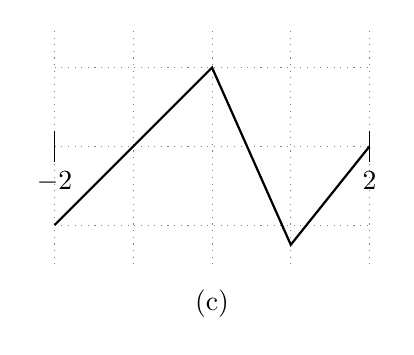
\begin{tikzpicture}
\YEaxis{2.25}{1.5}
\draw[thin, gray, dotted] (-2,-1.5) grid (2,1.5);
\draw (-2,.2)--(-2,-.2) node[below]{$-2$};
\draw (2,.2)--(2,-.2) node[below]{$2$};
\draw[thick] (-2,-1)--(0,1)--(1,-1.25)--(2,0);
\draw (0,-2) node{(c)};
\end{tikzpicture}
\end{center}
%
\begin{center}
\begin{tikzpicture}
\YEaxis{2.25}{1.5}
\draw[thin, gray, dotted] (-2,-1.5) grid (2,1.5);
\draw (-2,.2)--(-2,-.2) node[below]{$-2$};
\draw (2,.2)--(2,-.2) node[below]{$2$};
\draw[thick] (-2,1)--(2,1);
\draw (0,-2) node{(d)};
\end{tikzpicture}\hfill
\begin{tikzpicture}
\YEaxis{2.25}{1.5}
\draw[thin, gray, dotted] (-2,-1.5) grid (2,1.5);
\draw (-2,.2)--(-2,-.2) node[below]{$-2$};
\draw (2,.2)--(2,-.2) node[below]{$2$};
\draw[thick] (-2,0)--(2,1);
\draw (0,-2) node{(e)};
\end{tikzpicture}\hfill
\begin{tikzpicture}
\YEaxis{2.25}{1.5}
\draw[thin, gray, dotted] (-2,-1.5) grid (2,1.5);
\draw (-2,.2)--(-2,-.2) node[below]{$-2$};
\draw (2,.2)--(2,-.2) node[below]{$2$};
\draw[thick] (-2,1)--(-1,-1)--(1,-1)--(2,0);
\draw (0,-2) node{(f)};
\end{tikzpicture}
\end{center}
\end{question}
\begin{hint} Your calculations for slope of the secant lines will all have the same denominators; to save yourself some time, you can focus on the numerators.
\end{hint}
\begin{answer} \{(a), (c), (e)\}, \quad\{(b),(f)\},\quad \{(d)\}
\end{answer}
\begin{solution} The slope of the secant line will be $\dfrac{f(2)-f(-2)}{2-(-2)} = \dfrac{f(2)-f(-2)}{4}$, in every part. So, if two lines have the same slope, that means their differences $f(2)-f(-2)$ will be the same.

The graphs in (a),(c), and (e) all have $f(2)-f(-2)=1$, so they all have the same secant line slope. The graphs in (b) and (f) both have $f(2)-f(-2)=-1$, so they both have the same secant line slope. The graph in (d) has $f(2)-f(-2)=0$, and it is the only graph with this property, so it does not share its secant line slope with any of the other graphs.
\end{solution}


%%%%%%%%%%%%%%%%%%
\subsection*{\Procedural}
%%%%%%%%%%%%%%%%%%


\begin{question}
Give your best approximation of the slope of the tangent line to
the graph below at the point $x=5$.
\begin{center}
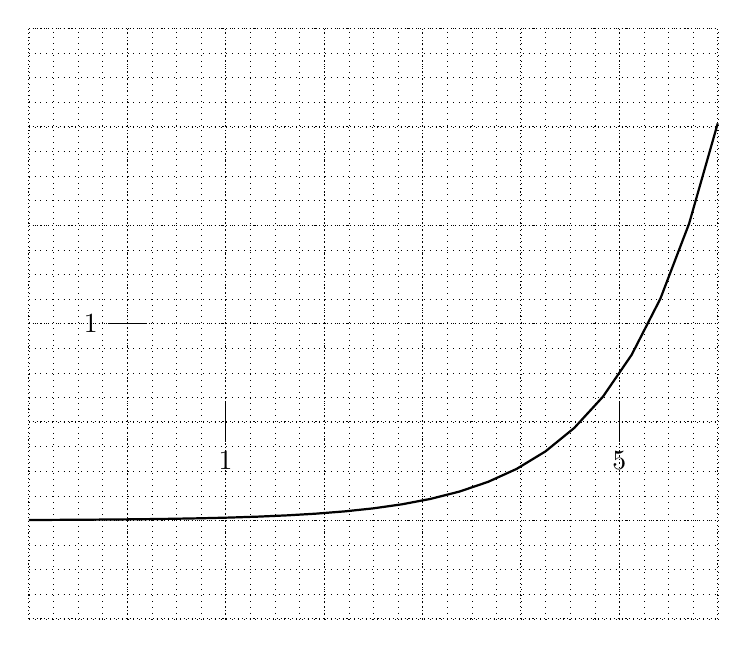
\begin{tikzpicture}[scale=1.25]
\YEaaxis{1.1}{6.1}{2.1}{4.1}
\draw[densely dotted] (-1,-2) grid (6,4);
\draw (1,.2)--(1,-.2) node[below]{1};
\draw (5,.2)--(5,-.2) node[below]{5};
\draw (.2,1)--(-.2,1) node[left]{1};
\draw[dotted, ultra thin] (-1,-2) grid[step=.25] (6,4);
\draw[thick] plot[domain=-1:6](\x,{exp(\x)/100-1});
\end{tikzpicture}
\end{center}
\end{question}
\begin{hint} You can do this by calculating several secant lines. You can also do this by getting out a ruler and trying to draw the tangent line very carefully.
\end{hint}
\begin{answer} Something like $1.5$. A reasonable answer would be between 1 and 2.
\end{answer}
\begin{solution} A good approximation from the graph is $f(5)=0.5$. We want to find a secant line whose endpoints are both very close to $x=5$, but that also give us clear $y$-values. It looks like $f(5.25) \approx 1$, and $f(4.75)\approx \frac{1}{8}$. The secant line from $x=5$ to $x=5.25$ has approximate slope $\dfrac{f(5.25)-f(5)}{5.25-5}\approx \dfrac{1-.5}{.25}=2$. The secant line from $x=5$ to $x=4.75$ has approximate slope $\dfrac{0.5-\frac{1}{8}}{5-4.75}=\dfrac{3}{2}$.

The graph increases more and more quickly (gets steeper and steeper), so it makes sense that the secant line to the left of $x=5$ has a smaller slope than the secant line to the right of $x=5$.  Also, if you're taking secant lines that have endpoints farther out from $x=5$, you'll notice that the slopes of the secant lines change quite dramatically. You have to be very, very close to $x=5$ to get any kind of accuracy.

If we split the difference, we might approximate the slope of the secant line to be the average of $\frac{3}{2}$ and $2$, which is $\frac{7}{4}$.

Another way to try to figure out the tangent line is by carefully drawing it in with a ruler. This is shown here in blue:
\begin{center}
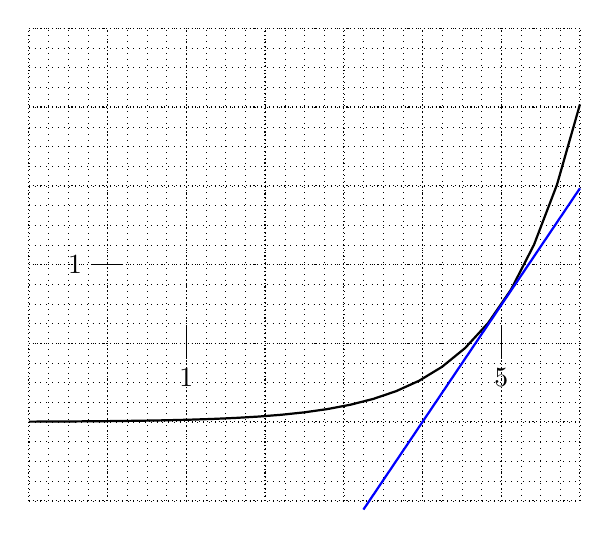
\begin{tikzpicture}
\YEaaxis{1.1}{6.1}{2.1}{4.1}
\draw[densely dotted] (-1,-2) grid (6,4);
\draw (1,.2)--(1,-.2) node[below]{1};
\draw (5,.2)--(5,-.2) node[below]{5};
\draw (.2,1)--(-.2,1) node[left]{1};
\draw[dotted, ultra thin] (-1,-2) grid[step=.25] (6,4);
\draw[thick] plot[domain=-1:6](\x,{exp(\x)/100-1});
\draw[thick, blue] plot[domain=3.25:6](\x,{1.484*(\x-5)+.484});
\end{tikzpicture}
\end{center}
It's much easier to take the slope of a line than a curve, and this one looks like it has slope about 1.5. However, we drew this with a computer: by hand it's much harder to draw an accurate tangent line. (That's why we need calculus!)

The actual slope of the tangent line to the function at $x=5$ is about $1.484$. This is extremely hard to figure out just from the graph--by hand, a guess between $1.25$ and $1.75$ would be very accurate.
\end{solution}


\begin{Mquestion}On the graph below, sketch the tangent line to $y=f(x)$ at $P$. Then, find two points $Q$ and $R$  on the graph so that the secant line through $Q$ and $R$ has the same slope as the tangent line at $P$.
\begin{center}
\begin{tikzpicture}
\YEaxis{5}{3}
\draw[thick] plot[domain=0:4.5](\x,{\x*\x/4-2}) node[below right]{$y=f(x)$};
\draw[thick] (-4.5,0) cos (-2.25,-1) sin (0,-2);
\draw (1,-7/4) node[vertex, label=below:$P$]{};
\end{tikzpicture}
\end{center}
\end{Mquestion}
\begin{hint} There are many possible values for $Q$ and $R$.
\end{hint}
\begin{answer} There is only one tangent line to $f(x)$ at $P$ (shown in blue), but there are infinitely many choices of $Q$ and $R$ (one possibility shown in red).
\begin{center}
\begin{tikzpicture}
\YEaxis{5}{3}
\draw[thick] plot[domain=0:4.5](\x,{\x*\x/4-2}) node[below right]{$y=f(x)$};
\draw[thick] (-4.5,0) cos (-2.25,-1) sin (0,-2);
\draw (1,-7/4) node[vertex, label=below:$P$]{};
\draw[blue, thick] (-1,-11/4)--(4,-1/4);
\draw[red] (0,-2) node[vertex, label=above left:$Q$]{};
\draw[red] (2,-1) node[vertex, label=above:$R$]{};
\draw[red, thick] (-1,-2.5)--(4,0);
\end{tikzpicture}
\end{center}
\end{answer}
\begin{solution} There is only one tangent line to $f(x)$ at $P$ (shown in blue), but there are infinitely many choices of $Q$ and $R$ (one possibility shown in red).
One easy way to sketch the secant line on paper is to draw any line parallel to the tangent line, and choose two intercepts with $y=f(x)$.
\begin{center}
\begin{tikzpicture}
\YEaxis{5}{3}
\draw[thick] plot[domain=0:4.5](\x,{\x*\x/4-2}) node[below right]{$y=f(x)$};
\draw[thick] (-4.5,0) cos (-2.25,-1) sin (0,-2);
\draw (1,-7/4) node[vertex, label=below:$P$]{};
\draw[blue, thick] (-1,-11/4)--(4,-1/4);
\draw[red] (0,-2) node[vertex, label=above left:$Q$]{};
\draw[red] (2,-1) node[vertex, label=above:$R$]{};
\draw[red, thick] (-1,-2.5)--(4,0);
\end{tikzpicture}
\end{center}
\end{solution}


\begin{Mquestion}Mark the points where the curve shown below has a tangent line with slope $0$.
\begin{center}
\begin{tikzpicture}
\YEaxis{5}{3}
\draw[thick] plot[domain=2:4.5](\x,{-(\x-3)*(\x-3)/2-1/2}) node[below right]{$y=f(x)$};
\draw[thick] plot[domain=-1:2](\x,{\x*\x/4-2});
\draw[thick] plot[smooth] coordinates{(-5,3) (-4,1.3) (-3,1) (-2,-1) (-1,-7/4)};
\end{tikzpicture}\end{center}
(Later on, we'll learn how these points tell us a lot about the shape of a graph.)
\end{Mquestion}
\begin{hint} A line with slope $0$ is horizontal.
\end{hint}
\begin{answer}
\begin{center}
\begin{tikzpicture}
\YEaxis{5}{3}
\draw[thick] plot[domain=2:4.5](\x,{-(\x-3)*(\x-3)/2-1/2}) node[below right]{$y=f(x)$};
\draw[thick] plot[domain=-1:2](\x,{\x*\x/4-2});
\draw[thick] plot[smooth] coordinates{(-5,3) (-4,1.3) (-3,1) (-2,-1) (-1,-7/4)};
\draw[blue] (-3.5,1.15) node[vertex]{};
\draw[blue] (0,-2) node[vertex]{};
\draw[blue] (3,-1/2) node[vertex]{};
\end{tikzpicture}\end{center}
\end{answer}
\begin{solution}
Any place the graph looks flat (if you imagine zooming in) is where the tangent line has slope 0. This occurs three times.
\begin{center}
\begin{tikzpicture}
\YEaxis{5}{3}
\draw[thick] plot[domain=2:4.5](\x,{-(\x-3)*(\x-3)/2-1/2}) node[below right]{$y=f(x)$};
\draw[thick] plot[domain=-1:2](\x,{\x*\x/4-2});
\draw[thick] plot[smooth] coordinates{(-5,3) (-4,1.3) (-3,1) (-2,-1) (-1,-7/4)};
\draw[blue] (-3.5,1.15) node[vertex]{};
\draw[blue] (0,-2) node[vertex]{};
\draw[blue] (3,-1/2) node[vertex]{};
\end{tikzpicture}\end{center}
Notice that two of the indicated points are at a low point and a high point, respectively. Later, we'll use these places where the tangent line has slope zero to find where a graph achieves its biggest and smallest values.
\end{solution}

\section{Definition of the derivative}
%
% Copyright 2018 Joel Feldman, Andrew Rechnitzer and Elyse Yeager.
% This work is licensed under a Creative Commons Attribution-NonCommercial-ShareAlike 4.0 International License.
% https://creativecommons.org/licenses/by-nc-sa/4.0/
%
\questionheader{ex:s2.2}
%%%%%%%%%%%%%%%%%%
\subsection*{\Conceptual}
%%%%%%%%%%%%%%%%%%


\begin{question}
The function $f(x)$ is shown. Select all options below that describe its derivative, $\ds\diff{f}{x}$:
\begin{center}
(a) constant \qquad (b) increasing
\qquad (c) decreasing\\
(d) always positive
\qquad (e) always negative

\begin{tikzpicture}
\YEaxis{5}{3}
\draw[thick] plot[domain=-4:4](\x,{\x/5*3}) node[below right]{$y=f(x)$};
\end{tikzpicture}
\end{center}
\end{question}
\begin{hint} What are the properties of $f'$ when $f$ is a line?
\end{hint}
\begin{answer}(a), (d)
\end{answer}
\begin{solution} The function shown is a line, so it has a constant slope--(a) . Since the function is always increasing, $f'$ is always positive, so also (d) holds. Remark: it does not matter that the function itself is sometimes negative; the slope is always positive because the function is always increasing. Also, since the slope is constant, $f'$ is neither increasing nor decreasing: it is the \emph{function} that is increasing, not its derivative.
\end{solution}


\begin{question}
The function $f(x)$ is shown. Select all options below that describe its derivative, $\ds\diff{f}{x}$:
\begin{center}
(a) constant \qquad (b) increasing
\qquad (c) decreasing\\
 (d) always positive
\qquad (e) always negative

\begin{tikzpicture}
\YEaxis{5}{3}
\draw[thick] plot[smooth] coordinates{(-4,3) (-3,2.75) (-2,2) (-1,1.75) (0,1)};
\draw[thick] plot[domain=0:4](\x,{exp(-\x)})node[below right]{$y=f(x)$};
\end{tikzpicture}
\end{center}
\end{question}
\begin{hint} Be very careful not to confuse $f$ and $f'$.
\end{hint}
\begin{answer} (e)
\end{answer}
\begin{solution} The function is always decreasing, so $f'$ is always negative, option (e). However, the function alternates between being more and less steep, so $f'$ alternates between increasing and decreasing several times, and no other options hold.

 Remark: $f$ is always positive, but (d) does not hold!
\end{solution}


\begin{Mquestion}
The function $f(x)$ is shown. Select all options below that describe its derivative, $\ds\diff{f}{x}$:
\begin{center}
(a) constant \qquad (b) increasing
\qquad (c) decreasing\\ (d) always positive
\qquad (e) always negative

\begin{tikzpicture}
\YEaxis{5}{3}
\draw[thick] plot[domain=-4:4](\x,{\x*\x/25*9-3}) node[below right]{$y=f(x)$};
\end{tikzpicture}
\end{center}
\end{Mquestion}
\begin{hint} Be very careful not to confuse $f$ and $f'$.
\end{hint}
\begin{answer} (b)
\end{answer}
\begin{solution}
At the left end of the graph, $f$ is decreasing rapidly, so $f'$ is a strongly negative number. Then as we move towards $x=0$, $f$ decreases less rapidly, so $f'$ is a less strongly negative number. As we pass 0, $f$ increases, so $f'$ is a positive number. As we move to the right, $f$ increases more and more rapidly, so $f'$ is an increasing positive number. This description tells us that $f'$ increases for the entire range shown. So (b) holds, but not (a) or (c). Since $f'$ is negative to the left of the $y$ axis, and positive to the right of it, also (d) and (e) do not hold.
\end{solution}


\begin{question}[2006H]
State, in terms of a limit, what it means for
$f(x) = x^3$ to be differentiable at $x = 0$.
\end{question}
\begin{answer}
By definition, $f(x) = x^3$ is differentiable at $x = 0$
if the limit
$$
\lim_{h\rightarrow 0}\frac{f(h)-f(0)}{h}
=\lim_{h\rightarrow 0}\frac{h^3-0}{h}
$$
exists.
\end{answer}
\begin{solution}
By definition, $f(x) = x^3$ is differentiable at $x = 0$
if the limit
$$
\lim_{h\rightarrow 0}\frac{f(h)-f(0)}{h}
=\lim_{h\rightarrow 0}\frac{h^3-0}{h}
$$
exists.
\end{solution}



\begin{Mquestion}For which values of $x$ does $f'(x)$ not exist?
\begin{center}
\begin{tikzpicture}
\YEaxis{5.2}{3.2}
\draw[thin, gray, dotted] (-5,-3) grid (5,3);
\draw[thick] (-5,-2) sin (-3,1) cos (-1,2)--(3,1);
\draw (3,1) node[vertex]{};
\draw (3,-2) node[opendot]{}--(5,-2.5);
\draw (1,.2)--(1,-.2) node[below]{1};
\draw (.2,1)--(-.2,1) node[left]{1};
\end{tikzpicture}
\end{center}
\end{Mquestion}
\begin{hint} The slope has to look ``the same" from the left and the right.
\end{hint}
\begin{answer} $x=-1$ and $x=3$
\end{answer}
\begin{solution}
$f'(-1)$ does not exist, because to the left of $x=-1$ the slope is a pretty big positive number (looks like around $+1$) and to the right the slope is $-1/4$. Since the derivative involves a limit, that limit needs to match the limit from the left and the limit from the right. The sharp angle made by the graph at $x=-1$ indicates that the left and right limits do not match, so the derivative does not exist.

$f'(3)$ also does not exist.  One way to see this is to notice that the function is discontinuous here. More viscerally, note that $f(3)=1$, so as we take secant lines with one endpoint $(3,1)$, and the other endpoint just to the right of $x=3$, we get slopes that are more and more strongly negative, as shown in the picture below. If we take the limit of the slopes of these secant lines as $x$ goes to $3$ from the right, we get $-\infty$. (This certainly doesn't match the slope from the left, which is $-\frac{1}{4}$.)
\begin{center}
\begin{tikzpicture}[scale=0.5]
\YEaxis{5.2}{3.2}
\draw[thin, gray, dotted] (-5,-3) grid (5,3);
\draw[thick] (-5,-2) sin (-3,1) cos (-1,2)--(3,1);
\draw (3,1) node[vertex]{};
\draw (3,-2) node[opendot]{}--(5,-2.5);
\draw (1,.2)--(1,-.2) node[below]{1};
\draw (.2,1)--(-.2,1) node[left]{1};
\draw[thick,orange] (3,1) --(4,-2.25) node[vertex]{};
\draw[thick,orange] (3,1) --(5,-2.5) node[vertex]{};
\draw[thick,red] (3,1) node[vertex]{}--(3.5,-2.125) node[vertex]{};
\end{tikzpicture}
\end{center}

At $x=-3$, there is some kind of ``change" in the graph; however, it is a smooth curve, so the derivative exists here.
\end{solution}


\begin{Mquestion}\label{s2.2onesided1}
Suppose $f(x)$ is a function defined at $x=a$ with \[\lim_{h \to 0^-}\frac{f(a+h)-f(a)}{h}=\lim_{h \to 0^+}\frac{f(a+h)-f(a)}{h}=1.\] True or false: $f'(a)=1$.
\end{Mquestion}
\begin{hint} Use the definition of the derivative, and what you know about limits.
\end{hint}
\begin{answer} True. (Contrast to Question~\ref{s2.2onesided2}.)
\end{answer}
\begin{solution}
True.
The definition of the derivative tells us that
\[f'(a) = \lim_{h \to 0}\dfrac{f(a+h)-f(a)}{h},\] if it exists. We know from our work with limits that if both one-sided limits\\
$\ds\lim_{h \to 0^-}\frac{f(a+h)-f(a)}{h}$ and $\ds\lim_{h \to 0^+}\frac{f(a+h)-f(a)}{h}$ exist and are equal to each other, then $\ds \lim_{h \to 0}\dfrac{f(a+h)-f(a)}{h}$ exists and has the same value as the one-sided limits. So, since the one-sided limits exist and are equal to one, we conclude $f'(a)$ exists and is equal to one.
\end{solution}

\begin{Mquestion}\label{s2.2onesided2}
Suppose $f(x)$ is a function defined at $x=a$ with
\[\lim_{x \to a^-}f'(x)=\lim_{x \to a^+}f'(x)=1.\] True or false: $f'(a)=1$.
\end{Mquestion}
\begin{hint} Consider continuity. \end{hint}
\begin{answer} In general, false. (Contrast to Question~\ref{s2.2onesided1}.)
\end{answer}
\begin{solution}
In general, this is false. The key problem that can arise is that $f(x)$ might not be continuous at $x=1$.  One example is the function
\[f(x)=\left\{\begin{array}{ll}
x&x<0\\
x-1&x \geq 0
\end{array}\right.\]
where $f'(x)=1$ whenever $x \neq 0$  (so in particular, $\ds\lim_{x \to 0^-}f'(x)=\ds\lim_{x \to 0^+} f'(x)=1$) but $f'(0)$ does not exist.

There are two ways to see that $f'(0)$ does not exist. One is to notice that $f$ is not continuous at $x=0$.

\begin{center}\begin{tikzpicture}
\YEaxis{3}{3}
\draw[thick] plot[domain=-3:0](\x,\x);
\draw node[opendot]{};
\draw[thick] plot[domain=0:3](\x,{\x-1}) node[right]{$y=f(x)$};
\draw (0,-1) node[vertex]{};
\end{tikzpicture}\end{center}

Another way to see that $f'(0)$ does not exist is to use the definition of the derivative. Remember, in order for a limit to exist, both one-sided limits must exist. Let's consider the limit from the left. If $h \to 0^-$, then $h<0$, so $f(h)$ is equal to $h$ (not $h-1$).

\begin{align*}
\lim_{h \to 0^-}\frac{f(0+h)-f(0)}{h}&=\lim_{h \to 0^-}\frac{(h)-(-1)}{h}\\
&=\lim_{h \to 0^-}\frac{h+1}{h}\\
&=\lim_{h \to 0^-}1+\frac{1}{h}\\
&=-\infty
\intertext{In particular, this limit does not exist. Since the one-sided limit does not exist,}
\lim_{h \to 0}\frac{f(0+h)-f(0)}{h}&=DNE
\end{align*}
and so $f'(0)$ does not exist.
\end{solution}



\begin{Mquestion}
Suppose $s(t)$ is a function, with $t$ measured in seconds, and $s$ measured in metres. What are the units of $s'(t)$?
\end{Mquestion}
\begin{hint}
Look at the definition of the derivative. Your answer will be a fraction.
\end{hint}
\begin{answer} metres per second
\end{answer}
\begin{solution}
Using the definition of the derivative,
\[s'(t)=\lim_{h \to 0}\frac{s(t+h)-s(t)}{h}\]
The units of the numerator are meters, and the units of the denominator are seconds (since the denominator comes from the change in the \emph{input} of the function). So, the units of $s'(t)$ are metres per second.

Remark: we learned that the derivative of a position function gives velocity. In this example, the position is given in metres, and the velocity is measured in metres per second.
\end{solution}




%%%%%%%%%%%%%%%%%%
\subsection*{\Procedural}
%%%%%%%%%%%%%%%%%%




\begin{question}Use the definition of the derivative to find the equation of the tangent line to the curve $y(x)=x^3+5$ at the point $(1,6)$.
\end{question}
\begin{hint} You need a point (given), and a slope (derivative).
\end{hint}
\begin{answer} $y-6=3(x-1)$, or $y=3x +3$
\end{answer}
\begin{solution}
We can use point-slope form to get the equation of the line, if we have a point and its slope. The point is given: $(1,6)$. The slope is the derivative:
\begin{align*}
y'(1)&=\lim_{h \rightarrow 0}\frac{y(1+h)-y(1)}{h}\\
&=\lim_{h \rightarrow 0}\frac{[(1+h)^3+5]-[1^3+5]}{h}\\
&=\lim_{h \rightarrow 0}\frac{[1+3h+3h^2+h^3+5]-[1+5]}{h}\\
&=\lim_{h \rightarrow 0}\frac{3h+3h^2+h^3}{h}\\
&=\lim_{h \rightarrow 0}{3+3h+h^2}\\
&=3
\end{align*}
So our slope is 3, which gives a line of equation
$y-6=3(x-1)$.
\end{solution}



\begin{question}Use the definition of the derivative to find the derivative of
$f(x)=\frac{1}{x}$.
\end{question}
\begin{hint} You'll need to add some fractions.
\end{hint}
\begin{answer} $\dfrac{-1}{x^2}$
\end{answer}
\begin{solution}
We set up the definition of the derivative.
\begin{align*}
f'(x)&=\lim_{h \rightarrow 0}\frac{f(x+h)-f(x)}{h}\\
&=\lim_{h \rightarrow 0}\frac{\frac{1}{x+h}-\frac{1}{x}}{h}\\
&=\lim_{h \rightarrow 0}\frac{\frac{x}{x(x+h)}-\frac{x+h}{x(x+h)}}{h}\\
&=\lim_{h \rightarrow 0}\frac{\frac{x-(x+h)}{x(x+h)}}{h}\\
&=\lim_{h \rightarrow 0}\frac{\frac{-h}{x(x+h)}}{h}\\
&=\lim_{h \rightarrow 0}\frac{-1}{x(x+h)}\\
&=\frac{-1}{x^2}
\end{align*}
\end{solution}


\begin{question}[2007H]
Let $f(x) = x|x|$.
Using the definition of the derivative, show that
$f(x)$ is differentiable at $x = 0$.
\end{question}
\begin{hint}
You don't have to take the limit from the left and right separately--things will cancel nicely.
\end{hint}
\begin{answer}
 By definition
$$
f'(0)=\lim_{h\rightarrow 0}\frac{f(h)-f(0)}{h}
     =\lim_{h\rightarrow 0}\frac{h|h|}{h}
     =\lim_{h\rightarrow 0}|h|=0
$$
In particular, the limit exists, so the derivative exists (and is equal to zero).
\end{answer}
\begin{solution}
 By definition
$$
f'(0)=\lim_{h\rightarrow 0}\frac{f(h)-f(0)}{h}
     =\lim_{h\rightarrow 0}\frac{h|h|}{h}
     =\lim_{h\rightarrow 0}|h|=0
$$
In particular, the limit exists, so the derivative exists (and is equal to zero).
\end{solution}




\begin{Mquestion}[1997A]Use the definition of the derivative to compute the derivative
of the function $f(x)=\frac{2}{x+1}$.
\end{Mquestion}
\begin{hint} You might have to add fractions
\end{hint}
\begin{answer} $\dfrac{-2}{(x+1)^2}$
\end{answer}
\begin{solution}
We set up the definition of the derivative.
\begin{align*}
f'(x)&=\lim_{h\rightarrow 0}\frac{f(x+h)-f(x)}{h}
=\lim_{h\rightarrow 0}\frac{1}{h}\Big(\frac{2}{x+h+1}
-\frac{2}{x+1}\Big)
=\lim_{h\rightarrow 0}\frac{2}{h}\ \frac{(x+1)-(x+h+1)}{(x+h+1)(x+1)}\cr
&=\lim_{h\rightarrow 0}\frac{2}{h}\ \frac{-h}{(x+h+1)(x+1)}
=\lim_{h\rightarrow 0}\frac{-2}{(x+h+1)(x+1)}
=\frac{-2}{(x+1)^2}
\end{align*}
\end{solution}



\begin{question}[1996D]
Use the definition of the derivative to compute the derivative
of the function $f(x)=\frac{1}{x^2+3}$.
\end{question}
\begin{answer} {$\dfrac{-2x}{[x^2+3]^2}$}
\end{answer}
\begin{solution}
\begin{align*}
f'(x)&=\lim_{h\rightarrow 0}\frac{f(x+h)-f(x)}{h}
=\lim_{h\rightarrow 0}\frac{1}{h}\Big(\frac{1}{(x+h)^2+3}
-\frac{1}{x^2+3}\Big)
=\lim_{h\rightarrow 0}\frac{1}{h}\frac{x^2-(x+h)^2}{[(x+h)^2+3][x^2+3]}\cr
&=\lim_{h\rightarrow 0}\frac{1}{h}\frac{-2xh-h^2}{[(x+h)^2+3][x^2+3]}
=\lim_{h\rightarrow 0}\frac{-2x-h}{[(x+h)^2+3][x^2+3]}
=\boxed{\frac{-2x}{[x^2+3]^2}}
\end{align*}
\end{solution}







\begin{question}Use the definition of the derivative to find the slope of the tangent line to the curve\\ $f(x)=x\log_{10}(2x+10)$ at the point $x=0$.
\end{question}
\begin{hint} Your limit should be easy.
\end{hint}
\begin{answer} 1
\end{answer}
\begin{solution} The slope of the tangent line is the derivative.
We set this up using the same definition of the derivative that we always do. This limit is hard to take for general $x$, but easy when $x=0$.
\begin{align*}
f'(0)&=\lim_{h \rightarrow 0} \frac{f(0+h)-f(0)}{h}\\
&=\lim_{h \rightarrow 0} \frac{h\log_{10}(2h+10)-0}{h}\\
&=\lim_{h \rightarrow 0} \log_{10}(2h+10)=\log_{10}(10)=1
\end{align*}
So, the slope of the tangent line is 1.
\end{solution}




\begin{question}[1998H]
Compute the derivative of $f(x)=\frac{1}{x^2}$ directly
from the definition.
\end{question}
\begin{hint} add fractions
\end{hint}
\begin{answer} $f'(x)=-\dfrac{2}{x^3}$
\end{answer}
\begin{solution}
\begin{align*}
f'(x)&=\lim_{h\rightarrow 0}\frac{f(x+h)-f(x)}{h}
=\lim_{h\rightarrow 0}\frac{\frac{1}{(x+h)^2}-\frac{1}{x^2}}{h}
=\lim_{h\rightarrow 0}\frac{x^2-(x+h)^2}{(x+h)^2x^2h}
=\lim_{h\rightarrow 0}\frac{-2xh-h^2}{(x+h)^2x^2h}\cr
&=\lim_{h\rightarrow 0}\frac{-2x-h}{(x+h)^2x^2}=\frac{-2x}{x^4}
=-\frac{2}{x^3}
\end{align*}
\end{solution}





\begin{Mquestion}[2006H]
Find the values of the constants $a$ and $b$ for which
\begin{align*}
f(x) = \left\{
\begin{array}{lc}
	 x^2 & x\le 2\\
               ax + b   & x > 2
               \end{array}\right.
\end{align*}
is differentiable everywhere.

Remark: In the text, you have already learned the derivatives of $x^2$ and $ax+b$. In this question, you are only asked to find the values of $a$ and $b$---not to justify how you got them---so you don't have to use the definition of the derivative. However, on an exam, you might be asked to justify your answer, in which case you would show how to differentiate the two branches of $f(x)$ using the definition of a derivative.
\end{Mquestion}
\begin{hint}
For $f$ to be differentiable at $x=2$, two things must be true: it must be continuous at $x=2$, and the derivative from the right must equal the derivative from the left.
\end{hint}
\begin{answer}
$a=4$, $b=-4$
\end{answer}
\begin{solution}
When $x$ is not equal to 2, then the function is differentiable-- the only place we have to worry about is when $x$ is exactly 2.

In order for $f$ to be differentiable at $x=2$, it must also
be continuous at $x=2$. This forces $x^2\big|_{x=2}=\big[ax+b\big]_{x=2}$
or \[2a+b=4.\]

In order for a limit to exist, the left- and right-hand limits must exist and be equal to each other. Since a derivative is a limit, in order for $f$ to be differentiable at $x=2$, the left hand
derivative of $ax+b$ at $x=2$ must be
the same as the right hand derivative of $x^2$ at $x=2$.
Since $ax+b$ is a line, its derivative is $a$ everywhere. We've already seen the derivative of $x^2$ is $2x$, so we need
\[a=2x\big|_{x=2}=4.\]

So, the values of $a$ and $b$ that makes $f$ differentiable everywhere are $a=4$ and $b=-4$.
\end{solution}





\begin{question}[2009H]
Use the definition of the derivative to compute
$f'(x)$ if $f(x) = \sqrt{1 + x}$. Where does $f'(x)$ exist?
\end{question}
\begin{hint}
After you plug in $f(x)$ to the definition of a derivative, you'll want to multiply and divide by the conjugate $\sqrt{1+x+h}+\sqrt{1+x}$.
\end{hint}
\begin{answer} $f'(x)=\dfrac{1}{2\sqrt{1+x}}$ when $x>-1$; $f'(x)$ does not exist when $x \leq -1$.
\end{answer}
\begin{solution}
We plug in $f(x)$ to the definition of a derivative. To evaluate the limit, we multiply and divide by the conjugate of the numerator, then simplify.
\begin{align*}
f'(x)=\lim\limits_{h\rightarrow 0}\frac{f(x+h)-f(x)}{h}
&=\lim\limits_{h\rightarrow 0}\frac{\sqrt{1+x+h}-\sqrt{1+x}}{h}\\
&=\lim\limits_{h\rightarrow 0}\frac{\sqrt{1+x+h}-\sqrt{1+x}}{h}
\left(\frac{\sqrt{1+x+h}+\sqrt{1+x}}{\sqrt{1+x+h}+\sqrt{1+x}}\right)\\
&=\lim\limits_{h\rightarrow 0}\frac{(1+x+h)-(1+x)}{h(\sqrt{1+x+h}+\sqrt{1+x})}\\
&=\lim\limits_{h\rightarrow 0}\frac{h}{h(\sqrt{1+x+h}+\sqrt{1+x})}\\
&=\lim\limits_{h\rightarrow 0}\frac{1}{\sqrt{1+x+h}+\sqrt{1+x}}\\
&=\frac{1}{\sqrt{1+x+0}+\sqrt{1+x}}=\frac{1}{2\sqrt{1+x}}
\end{align*}

The domain of the function is $[-1,\infty)$. In particular, $f(x)$ is defined when $x=-1$. However, $f'(x)$ is not defined when $x=-1$, so $f'(x)$ only exists over $(-1,\infty)$.

Remark: $\ds\lim_{x \to -1^+}f'(x)=\infty$, so the tangent line to $f(x)$ at the point $x=-1$ has a vertical slope.
\end{solution}




%%%%%%%%%%%%%%%%%%
\subsection*{\Application}
%%%%%%%%%%%%%%%%%%


\begin{question} Use the definition of the derivative to find the velocity of an object whose position is given by the function $s(t)=t^4-t^2$.
\end{question}
\begin{hint} From Section~\ref*{sec velocity}, %1.2
compare the definition of velocity to the definition of a derivative. When you're finding the derivative, you'll need to cancel a lot on the numerator, which you can do by expanding the polynomials.
\end{hint}
\begin{answer} $v(t)=4t^3-2t$
\end{answer}
\begin{solution}
From Section~\ref*{sec velocity}, %1.2
we see that the velocity is exactly the derivative.
\begin{align*}
v(t)&=\lim_{h \rightarrow 0}\frac{s(t+h)-s(t)}{h}\\
&=\lim_{h \rightarrow 0}\frac{(t+h)^4-(t+h)^2-t^4+t^2}{h}\\
&=\lim_{h \rightarrow 0}\frac{(t^4+4t^3h+6t^2h^2+4th^3+h^4)-(t^2+2th+h^2)-t^4+t^2}{h}
\\
&=\lim_{h \rightarrow 0}\frac{4t^3h+6t^2h^2+4th^3+h^4-2th-h^2}{h}
\\
&=\lim_{h \rightarrow 0}4t^3+6t^2h+4th^2+h^3-2t-h\\
&=4t^3-2t
\end{align*}
So, the velocity is given by $v(t)=4t^3-2t$.
\end{solution}


\begin{Mquestion}[2015Q]
 Determine whether the derivative of following function exists at
$x=0$.
\begin{align*}
f(x) &=\begin{cases}
  x \cos x & \text{ if }  x\ge 0\\
  \sqrt{x^2+x^4} & \text{ if } x< 0
\end{cases}
\end{align*}
You must justify your answer using the definition of a derivative.
\end{Mquestion}
\begin{hint} You'll need to look at limits from the left and right. The fact that $f(0)=0$ is useful for your computation. Recall that if $x<0$ then $\sqrt{x^2}=|x|=-x$.
\end{hint}
\begin{answer} No, it does not.
\end{answer}
\begin{solution}
The function is differentiable at $x=0$ if the following limit:
$$\lim_{x\to 0}\frac{f(x)-f(0)}{x-0} = \lim_{x\to 0}\frac{f(x)-0}{x}=\lim_{x\to
0} \frac{f(x)}{x}$$
exists (note that we used the fact that $f(0)=0$ as per the definition of the
first branch which includes the point $x=0$). We start by computing the left limit. For this computation, recall that if $x<0$ then $\sqrt{x^2}=|x|=-x$.
$$\lim_{x\to 0^-}\frac{f(x)}{x}=\lim_{x\to 0^-}\frac{\sqrt{x^2+x^4}}{x}=\lim_{x\to
0^-} \frac{\sqrt{x^2}\sqrt{1+x^2}}{x}=\lim_{x \rightarrow 0}\frac{-x\sqrt{1+x^2}}{x}=-1$$
Now, from the right:
$$\lim_{x\to 0^+}\frac{x\cos x}{x}=\lim_{x\to
0^+}\cos x = 1.$$
Since the limit from the left does not equal the limit from the right, the derivative does not exist at $x=0$.
\end{solution}


\begin{question}[2015Q]
 Determine whether the derivative of the following function exists at
$x=0$
\begin{align*}
f(x) &=\begin{cases}
  x \cos x & \text{ if }  x\le 0\\
  \sqrt{1+x}-1 & \text{ if } x> 0
\end{cases}
\end{align*}
You must justify your answer using the definition of a derivative.
\end{question}
\begin{hint} You'll need to look at limits from the left and right. The fact that $f(0)=0$ is useful for your computation.
\end{hint}
\begin{answer} No, it does not.
\end{answer}
\begin{solution}
The function is differentiable at $x=0$ if the following limit:
$$\lim_{x\to 0}\frac{f(x)-f(0)}{x-0} = \lim_{x\to 0}\frac{f(x)-0}{x}=\lim_{x\to
0} \frac{f(x)}{x}$$
exists (note that we used the fact that $f(0)=0$ as per the definition of the
first branch which includes the point $x=0$).

We start by computing the left limit.
\begin{align*}
\lim_{x\to 0^-}\frac{f(x)}{x}=\lim_{x\to 0^-} \frac{x\cos x}{x}
=\lim_{x\to 0^-} \cos x = 1.
\end{align*}
Now, from the right:
\begin{align*}
\lim_{x\to 0^+}\frac{\sqrt{1+x}-1}{x}
&= \lim_{x\to 0^+}\frac{\sqrt{1+x}-1}{x} \cdot \frac{\sqrt{1+x}+1}{\sqrt{1+x}+1} \\
&= \lim_{x\to 0^+} \frac{1+x-1}{x(\sqrt{1+x}+1)}
= \lim_{x\to 0^+} \frac{1}{\sqrt{1+x}+1} = \frac{1}{2}
\end{align*}
Since the limit from the left does not equal the limit from the right, the derivative
does
not exist at $x=0$.
\end{solution}


\begin{question}[2015Q]
Determine whether the derivative of the following function exists at
$x=0$
\begin{align*}
f(x) &=\begin{cases}
  x^3-7x^2 & \text{ if }  x\le 0\\
  x^3 \cos\left(\frac{1}{x}\right) & \text{ if } x> 0
\end{cases}
\end{align*}
You must justify your answer using the definition of a derivative.
\end{question}
\begin{hint} You'll need to look at limits from the left and right. The fact that $f(0)=0$ is useful for your computation.
\end{hint}
\begin{answer} Yes, it is.
\end{answer}
\begin{solution}
The function is differentiable at $x=0$ if the following limit:
\begin{align*}
\lim_{x\to 0}\frac{f(x)-f(0)}{x-0} = \lim_{x\to 0}\frac{f(x)-0}{x}=\lim_{x\to 0}
\frac{f(x)}{x}
\end{align*}
exists (note that we used the fact that $f(0)=0$ as per the definition of the first branch
which includes the point $x=0$). We compute left and right limits; so
\begin{align*}
\lim_{x\to 0^-}\frac{f(x)}{x}=\lim_{x\to 0^-}\frac{x^3-7x^2}{x}=\lim_{x\to 0^-}
x^2-7x=0
\end{align*}
and
\begin{align*}
\lim_{x\to 0^+}\frac{x^3\cos\left(\frac{1}{x}\right)}{x}=\lim_{x\to 0^+}x^2\cdot
\cos\left(\frac{1}{x}\right).
\end{align*}
This last limit equals $0$ by the Squeeze Theorem since
\begin{align*}
-1\le \cos\left(\frac{1}{x}\right)\le 1
\end{align*}
and so,
\begin{align*}
-x^2\le x^2\cdot \cos\left(\frac{1}{x}\right)\le x^2,
\end{align*}
where in these inequalities we used the fact that $x^2\ge 0$. Finally, since $\lim_{x\to 0^+}-x^2=\lim_{x\to 0^+}x^2=0$, the Squeeze Theorem
yields that also $\lim_{x\to 0^+}x^2\cos\left(\frac{1}{x}\right) =0$, as claimed.

Since the left and right limits match (they're both equal to $0$), we conclude that indeed
$f(x)$ is differentiable at $x=0$ (and its derivative at $x=0$ is actually equal to $0$).
\end{solution}


\begin{question}[2015Q]
Determine whether the derivative of the following function exists at
$x=1$
\begin{align*}
f(x) &=\begin{cases}
  4x^2-8x+4 & \text{ if }  x\le 1\\
  (x-1)^2\sin\left(\dfrac{1}{x-1}\right) & \text{ if } x> 1
\end{cases}
\end{align*}
You must justify your answer using the definition of a derivative.
\end{question}
\begin{hint} You'll need to look at limits from the left and right. The fact that $f(1)=0$ is useful for your computation.
\end{hint}
\begin{answer}
Yes, it is.
\end{answer}
\begin{solution}
The function is differentiable at $x=1$ if the following limit:
$$\lim_{x\to 1}\frac{f(x)-f(1)}{x-1} = \lim_{x\to 1}\frac{f(x)-0}{x-1}=\lim_{x\to 1}
\frac{f(x)}{x-1}$$
exists (note that we used the fact that $f(1)=0$ as per the definition of the first branch which includes the point $x=0$). We compute left and right limits; so
$$\lim_{x\to 1^-}\frac{f(x)}{x-1}=\lim_{x\to 1^-}\frac{4x^2-8x+4}{x-1}=\lim_{x\rightarrow 1^-}\frac{4(x-1)^2}{x-1} =\lim_{x\to 1^-} 4(x-1)=0$$
and
$$\lim_{x\to 1^+}\frac{(x-1)^2\sin\left(\frac{1}{x-1}\right)}{x-1}=\lim_{x\to 1^+}(x-1)\cdot \sin\left(\frac{1}{x-1}\right).$$
This last limit equals $0$ by the Squeeze Theorem since
$$-1\le \sin\left(\frac{1}{x-1}\right)\le 1$$
and so,
$$ -(x-1)\le (x-1)\cdot \sin\left(\frac{1}{x-1}\right)\le x-1,$$
where in these inequalities we used the fact that $x\to 1^+$ yields positive values for
$x-1$. Finally, since $\lim_{x\to 1^+}-x+1=\lim_{x\to 1^+}x-1=0$, the Squeeze Theorem
yields that also $\lim_{x\to 1^+}(x-1)\sin\left(\frac{1}{x-1}\right) =0$, as claimed.

Since the left and right limits match (they're both equal to $0$), we conclude that indeed $f(x)$ is differentiable at $x=1$ (and its derivative at $x=1$ is actually equal to $0$).
\end{solution}




\begin{Mquestion}
Sketch a function $f(x)$ with $f'(0)=-1$ that takes the following values:

~\begin{center}
\begin{tabular}{|c|c|c|c|c|c|c|c|c|c|c|c|}
\hline
$\mathbf{x}$&$-1$&$-\frac{1^{ }}{2_{ }}$&$-\frac{1}{4}$&$-\frac{1}{8}$
&$0$
&$\frac{1}{8}$&$\frac{1}{4}$&$\frac{1}{2}$&$1$\\
\hline
$\mathbf{f(x)}$&$-1$&$-\frac{1^{ }}{2_{ }}$&$-\frac{1}{4}$&$-\frac{1}{8}$
&$0$
&$\frac{1}{8}$&$\frac{1}{4}$&$\frac{1}{2}$&$1$\\ \hline
\end{tabular}\end{center}~

Remark: you can't always guess the behaviour of a function from its points, even if the points seem to be making a clear pattern.
\end{Mquestion}
\begin{hint} There's lots of room between $0$ and $\frac{1}{8}$; see what you can do with it.
\end{hint}
\begin{answer} Many answers are possible; here is one.
\begin{center}
\begin{tikzpicture}
\YEaxis{4.2}{4.2}
\foreach \x in {1,1/2,1/4,1/8,0}{
	\draw (4*\x,4*\x) node[vertex]{};
	\draw (-\x*4,-\x*4) node[vertex]{};}
\draw (4,.2)--(4,-.2) node[below]{1};
\draw (.2,4)--(-.2,4) node[left]{1};
\draw[thick] (-4,-4)--(-1/2,-1/2) (1/2,1/2)--(4,4);
\draw[thick] (-1/2,-1/2) sin (-1/4,1/4) cos (0,0) sin (1/4,-1/4) cos (1/2,1/2);
\end{tikzpicture}
\end{center}
\end{answer}
\begin{solution}
Many answers are possible; here is one.
\begin{center}
\begin{tikzpicture}
\YEaxis{4.2}{4.2}
\foreach \x in {1,1/2,1/4,1/8,0}{
	\draw (4*\x,4*\x) node[vertex]{};
	\draw (-\x*4,-\x*4) node[vertex]{};}
\draw (4,.2)--(4,-.2) node[below]{1};
\draw (.2,4)--(-.2,4) node[left]{1};
\draw[thick] (-4,-4)--(-1/2,-1/2) (1/2,1/2)--(4,4);
\draw[thick] (-1/2,-1/2) sin (-1/4,1/4) cos (0,0) sin (1/4,-1/4) cos (1/2,1/2);
\end{tikzpicture}
\end{center}
The key is to realize that the few points you're given suggest a pattern, but don't guarantee it. You only know nine points; anything can happen in between.
\end{solution}




\begin{question}Let $p(x)=f(x)+g(x)$, for some functions $f$ and $g$ whose derivatives exist. Use limit laws and the definition of a derivative to show that $p'(x)=f'(x)+g'(x)$.

Remark: this is called the sum rule, and we'll learn more about it in Lemma~\ref*{thm:DIFFaddsub}.
\end{question}
\begin{hint} Set up your usual limit, then split it into two pieces
\end{hint}
\begin{answer}\begin{align*}
p'(x) &= \lim_{h \rightarrow 0} \frac{p(x+h)-p(x)}{h}\\
&= \lim_{h \rightarrow 0} \frac{f(x+h)+g(x+h)-f(x)-g(x)}{h}\\
&= \lim_{h \rightarrow 0} \frac{f(x+h)-f(x)+g(x+h)-g(x)}{h}\\
&= \lim_{h \rightarrow 0} \left[\frac{f(x+h)-f(x)}{h}+
\frac{g(x+h)-g(x)}{h}\right]\\
(*)&= \left[\lim_{h \rightarrow 0} \frac{f(x+h)-f(x)}{h}\right]+ \left[\lim_{h \rightarrow 0}
\frac{g(x+h)-g(x)}{h}\right]\\
&= f'(x)+g'(x)
\end{align*}
At step ($*$), we use the limit law that $\displaystyle\lim_{x \rightarrow a} \left[F(x)+G(x)\right] = \displaystyle\lim_{x \rightarrow a} F(x)+\displaystyle\lim_{x \rightarrow a}G(x)$, as long as  $\displaystyle\lim_{x \rightarrow a} F(x)$ and $\displaystyle\lim_{x \rightarrow a}G(x)$ exist. Because the problem states that $f'(x)$ and $g'(x)$ exist, we know that $\displaystyle\lim_{h \rightarrow 0} \frac{f(x+h)-f(x)}{h}$ and $\displaystyle\lim_{h \rightarrow 0}
\frac{g(x+h)-g(x)}{h}$ exist, so our work is valid.
\end{answer}
\begin{solution}
\begin{align*}
p'(x) &= \lim_{h \rightarrow 0} \frac{p(x+h)-p(x)}{h}\\
&= \lim_{h \rightarrow 0} \frac{f(x+h)+g(x+h)-f(x)-g(x)}{h}\\
&= \lim_{h \rightarrow 0} \frac{f(x+h)-f(x)+g(x+h)-g(x)}{h}\\
&= \lim_{h \rightarrow 0}\left[ \frac{f(x+h)-f(x)}{h}+
\frac{g(x+h)-g(x)}{h}\right]\\
(*)&= \left[\lim_{h \rightarrow 0} \frac{f(x+h)-f(x)}{h}\right]+ \left[\lim_{h \rightarrow 0}
\frac{g(x+h)-g(x)}{h}\right]\\
&= f'(x)+g'(x)
\end{align*}
At step ($*$), we use the limit law that $\displaystyle\lim_{x \rightarrow a} \left[F(x)+G(x)\right] = \displaystyle\lim_{x \rightarrow a} F(x)+\displaystyle\lim_{x \rightarrow a}G(x)$, as long as  $\displaystyle\lim_{x \rightarrow a} F(x)$ and $\displaystyle\lim_{x \rightarrow a}G(x)$ exist. Because the problem states that $f'(x)$ and $g'(x)$ exist, we know that $\displaystyle\lim_{h \rightarrow 0} \frac{f(x+h)-f(x)}{h}$ and $\displaystyle\lim_{h \rightarrow 0}
\frac{g(x+h)-g(x)}{h}$ exist, so our work is valid.
\end{solution}


\begin{question}Let $f(x)=2x$, $g(x)=x$, and $p(x)=f(x) \cdot g(x)$.
\begin{enumerate}[(a)]
\item\label{s2.2prod1} Find $f'(x)$ and $g'(x)$.
\item\label{s2.2prod2} Find $p'(x)$.
\item\label{s2.2prod3} Is $p'(x)=f'(x) \cdot g'(x)$?
\end{enumerate}
In Theorem~\ref*{thm:DIFFprodRule}, you'll learn a rule for calculating the derivative of a product of two functions.
\end{question}
\begin{hint} You don't need the definition of the derivative for a line.\end{hint}
\begin{answer}
\eqref{s2.2prod1} $f'(x)=2$ and $g'(x)=1$
\qquad \eqref{s2.2prod2} $p'(x)=4x$
\qquad \eqref{s2.2prod3} no
\end{answer}
\begin{solution}
\eqref{s2.2prod1}
Since $y=f(x)=2x$ and $y=g(x)=x$ are straight lines, we don't need the definition of the derivative (although you can use it if you like). $f'(x)=2$ and $g'(x)=1$.

\eqref{s2.2prod2} $p(x)=2x^2$, so $p(x)$ is not a line: we use the definition of a derivative to find $p'(x)$.
\begin{align*}
p'(x)&=\lim_{h \rightarrow 0} \frac{p(x+h)-p(x)}{h}\\
&=\lim_{h \rightarrow 0} \frac{2(x+h)^2-2x^2}{h}\\
&=\lim_{h \rightarrow 0} \frac{2x^2+4xh+2h^2-2x^2}{h}\\
&=\lim_{h \rightarrow 0} \frac{4xh+2h^2}{h}\\
&=\lim_{h \rightarrow 0} {4x+2h}\\&=4x
\end{align*}

\eqref{s2.2prod3} No, $p'(x) = 4x \ne 2\cdot 1 = f'(x)\cdot g'(x)$. In general, the derivative of a product is not the same as the derivative of the functions being multiplied.
\end{solution}


\begin{Mquestion}[2006H]
There are two distinct straight lines that pass
through the point $(1,-3)$ and are tangent to the curve $y = x^2$.
Find equations for these two lines.

Remark: the point $(1,-3)$ does not lie on the curve $y=x^2$.
\end{Mquestion}
\begin{hint}
A generic point on the curve has coordinates $(\alpha, \alpha^2)$. In terms of $\alpha$, what is the equation of the tangent line to the curve at the point $(\alpha, \alpha^2)$? What does it mean for $(1,-3)$ to be on that line?
\end{hint}
\begin{answer}
$y=6x-9$ and $y=-2x-1$
\end{answer}
\begin{solution}
We know that $y'=2x$. So, if we choose a point $(\alpha,\alpha^2)$ on the curve $y=x^2$,
then the tangent line to the curve at that point has slope $2\alpha$. That is, the tangent line has equation
\begin{align*}
(y-\alpha^2)&=2\alpha(x-\alpha)\\
\mbox{simplified, } \qquad y&=(2\alpha)x-\alpha^2
\intertext{So, if $(1,-3)$ is on the tangent line, then}
-3&=(2\alpha)(1)-\alpha^2\\
\iff\qquad 0&=\alpha^2-2\alpha-3\\
\iff\qquad 0&=(\alpha-3)(\alpha+1)\\
\iff\qquad \alpha&=3, \quad\mbox{or}\qquad \alpha=-1.
\intertext{So, the tangent lines  $y=(2\alpha)x-\alpha^2$ are}
y&=6x-9 \quad\mbox{and}\quad y=-2x-1.
\end{align*}
\end{solution}


\begin{question}[2009H]
 For which values of $a$ is the function
\[
f(x) =\left\{\begin{array}{ll}
	0 & x\le 0\\
             x^a \sin\frac{1}{x} & x > 0\end{array}\right.
\]
differentiable at 0?
\end{question}
\begin{hint}
Remember for a constant $n$, \[\ds\lim_{h \to 0} h^{n} = \left\{\begin{array}{ll}
0&n>0\\
1&n=0\\
DNE&n<0
\end{array}\right.\]
\end{hint}
\begin{answer} $a>1$
\end{answer}
\begin{solution}
Using the definition of the derivative, $f$ is differentiable at $0$ if and only if
\begin{align*}
\lim_{h \to 0}\frac{f(h)-f(0)}{h}&
\intertext{exists. In particular, this means $f$ is differentiable at $0$ if and only if both one-sided limits exist and are equal to each other. }\intertext{When $h<0$, $f(h)=0$, so}
\lim_{h \to 0^-}\frac{f(h)-f(0)}{h}&=\lim_{h \to 0^-}\frac{0-0}{h}=0
\intertext{So, $f$ is differentiable at $x=0$ if and only if}
\lim_{h \to 0^+}\frac{f(h)-f(0)}{h}&=0.
\intertext{ To evaluate the  limit above, we note $f(0)=0$ and, when $h>0$, $f(h)=h^a\sin\left(\frac{1}{h}\right)$, so}
\lim_{h \to 0^+}\frac{f(h)-f(0)}{h}&=\lim_{h \to 0^+}\frac{h^a\sin\left(\frac{1}{h}\right)}{h}\\
&=\lim_{h \to 0^+}h^{a-1}\sin\left(\frac{1}{h}\right)
\intertext{We will spend the rest of this solution evaluating the limit above for different values of $a$, to find when it is equal to zero and when it is not. Let's consider the different values that could be taken by $h^{a-1}$.}
\end{align*}
\begin{itemize}
\item If $a=1$, then $a-1=0$, so $h^{a-1}=h^0=1$ for all values of $h$. Then
\[\lim_{h \to 0^+}h^{a-1}\sin\left(\frac{1}{h}\right)=\lim_{h \to 0^+}\sin\left(\frac{1}{h}\right)=DNE\]
(Recall that the function $\sin\left(\frac{1}{x}\right)$ oscillates faster and faster as $x$
goes to 0. We first saw this behaviour in Example~\ref*{eg sinpix}.)

\item If $a<1$, then $a-1<0$, so $\ds\lim_{h \to 0^+}h^{a-1}=\infty$. (Since we have a negative exponent, we are in effect \emph{dividing  by} a smaller and smaller positive number. For example, if $a=\frac{1}{2}$, then $\ds\lim_{h \to 0^+}h^{a-1}=\ds\lim_{h \to 0^+}h^{-\frac{1}{2}}=\ds\lim_{h \to 0^+}\frac{1}{\sqrt{h}}=\infty$.) Since $\sin\left(\frac{1}{x}\right)$ goes back and forth between one and negative one,
\[\lim_{h \to 0^+}h^{a-1}\sin\left(\frac{1}{x}\right)=DNE\]
since as $h$ goes to 0, the function oscillates between positive and negative numbers of ever-increasing magnitude.

\item If $a>1$, then $a-1>0$, so $\ds\lim_{h \to 0^+}h^{a-1}=0$. Although $\sin\left(\frac{1}{x}\right)$ oscillates wildly near $x=0$, it is bounded by $-1$ and $1$. So,
\[(-1)h^{a-1} \leq h^{a-1}\sin\left(\frac{1}{h}\right) \leq h^{a-1}\]
Since both $\ds\lim_{h \to 0^+} (-1)h^{a-1}=0$ and $\ds\lim_{h \to 0^+} h^{a-1}=0$, by the Squeeze Theorem, \[\ds\lim_{h \to 0^+} h^{a-1}\sin\left(\frac{1}{x}\right)=0\] as well.
\end{itemize}

In the above cases, we learned \\
$\ds\lim_{h \to 0^+}\frac{f(h)-f(0)}{h}=\ds\lim_{h \to 0^+} h^{a-1}\sin\left(\frac{1}{x}\right)=0$ when $a>1$, and \\
$\ds\lim_{h \to 0^+}\frac{f(h)-f(0)}{h}=\ds\lim_{h \to 0^+} h^{a-1}\sin\left(\frac{1}{x}\right)\neq 0$ when $a \leq 1$.\\
So, $f$ is differentiable at $x=0$ if and only if $a>1$.
\end{solution}

\section{Interpretations of the derivative}
%
% Copyright 2018 Joel Feldman, Andrew Rechnitzer and Elyse Yeager.
% This work is licensed under a Creative Commons Attribution-NonCommercial-ShareAlike 4.0 International License.
% https://creativecommons.org/licenses/by-nc-sa/4.0/
%
\questionheader{ex:s2.3}
%%%%%%%%%%%%%%%%%%
\subsection*{\Procedural}
%%%%%%%%%%%%%%%%%%


\begin{Mquestion}
Suppose $h(t)$ gives the height at time $t$ of the water at a dam, where the units of $t$ are hours and the units of $h$ are meters.
\begin{enumerate}[(a)]
\item\label{s2.1dam1} What is the physical interpretation of the slope of the secant line through the points $(0,h(0))$ and $(24,h(24))$?
\item\label{s2.1dam2} What is the physical interpretation of the slope of the tangent line to the curve $y=h(t)$ at the point $(0,h(0))$?
\end{enumerate}
\end{Mquestion}
\begin{hint}
Think about units.
\end{hint}
\begin{answer}
\eqref{s2.1dam1} The average rate of change of the height of the water over the single day starting at $t=0$, measured in $\frac{\mathrm{m}}{\mathrm{hr}}$.

\eqref{s2.1dam2} The instantaneous rate of change of the height of the water at the time $t=0$.
\end{answer}
\begin{solution}
\eqref{s2.1dam1} The slope of the secant line is $\dfrac{h(24)-h(0)}{24-0} \quad \dfrac{\mathrm{m}}{\mathrm{hr}}$; this is the change in height over the first day divided by the number of hours in the first day. So, it is the average rate of change of the height over the first day, measured in meters per hour.

\eqref{s2.1dam2} Consider \eqref{s2.1dam1}. The secant line gives the \emph{average} rate of change of the height of the dam; as we let the second point of the secant line get closer and closer to $(0,h(0))$, its slope approximates the instantaneous rate of change of the height of the water. So the slope of the tangent line is the  instantaneous rate of change of the height of the water at the time $t=0$, measured in $\frac{\mathrm{m}}{\mathrm{hr}}$.
\end{solution}

\begin{question}Suppose $p(t)$ is a function that gives the profit generated by selling $t$ widgets. What is the practical interpretation of $p'(t)$?
\end{question}
\begin{answer} Profit per widget
\end{answer}
\begin{solution}
$p'(t) = \displaystyle\lim_{h \rightarrow 0}\frac{p(t+h)-p(t)}{h} \approx \frac{p(t+1)-p(t)}{1} = p(t+1)-p(t)$, or the difference in profit caused by the sale of the $(t+1)^{\mathrm{st}}$ widget. So, $p'(t)$ is the profit from the $(t+1)^{\mathrm{st}}$ widget, so $p'(t)$ is the profit per widget.
\end{solution}

\begin{question} $T(d)$ gives the temperature of water at a particular location $d$ metres below the surface. What is the physical interpretation of $T'(d)$? Would you expect $T'(d)$ to be higher when $d$ is near 0, or when $d$ is very large?
\end{question}
\begin{answer} $T'(d)$ measures how quickly the temperature is changing per unit change of depth, measured in degrees per metre. $T'(d)$ will probably be largest when $d$ is near zero, unless there are hot springs or other underwater heat sources.
\end{answer}
\begin{solution} How quickly the temperature is changing per unit change of depth, measured in degrees per metre. In an ordinary body of water, the temperature near the surface ($d=0$) is pretty variable, depending on the sun, but deep down it is more stable (unless there are heat sources). So, one might reasonably expect that $T'(d)$ is larger when $d$ is near 0.
\end{solution}

\begin{question}$C(w)$ gives the calories in $w$ grams of a particular dish. What does $C'(w)$ describe?
\end{question}
\begin{answer} Calories per gram.
\end{answer}
\begin{solution} $C'(w)=\displaystyle\lim_{h \rightarrow 0} \dfrac{C(w+h)-C(w)}{h} \approx \dfrac{C(w+1)-C(w)}{1}=C(w+1)-C(w)$, which is the number of calories in $C(w+1)$ grams minus the number of calories in $C(w)$ grams. This is the number of calories per gram.
\end{solution}

\begin{Mquestion}The velocity of a moving object at time $t$ is given by $v(t)$. What is $v'(t)$?
\end{Mquestion}
\begin{answer} The acceleration of the object.
\end{answer}
\begin{solution} The rate of change of velocity is acceleration. (If your velocity is increasing, you're accelerating; if your velocity is decreasing, you have negative acceleration.)
\end{solution}


\begin{Mquestion}
The function $T(j)$ gives the temperature in degrees Celsius of a cup of water after $j$ joules of heat have been added. What is $T'(j)$?
\end{Mquestion}
\begin{answer} Degrees Celsius temperature change per joule of heat added.
(This is closely related to heat capacity and to
         specific heat --- there's a nice explanation of this on Wikipedia.)
\end{answer}
\begin{solution}
The rate of change in this case will be the relationship between the heat added and the temperature change. $\displaystyle\lim_{h \rightarrow 0} \dfrac{T(j+h)-T(j)}{h} \approx \dfrac{T(j+1)-T(j)}{1}=T(j+1)-T(j)$, or the change in temperature after the application of one joule. (This is closely related to heat capacity and to
         specific heat --- there's a nice explanation of this on Wikipedia.)
\end{solution}


\begin{Mquestion}\label{s2.3bacteria}A population of bacteria, left for a fixed amount of time at temperature $T$, grows to $P(T)$ individuals. Interpret $P'(T)$.
\end{Mquestion}
\begin{answer} Number of bacteria added per degree. That is: the number of extra bacteria (possibly negative) that will exist in the population by raising the temperature by one degree.
\end{answer}
\begin{solution} As usual, it is instructive to think about the definition of the derivative:
\[P'(T) = \displaystyle\lim_{h \rightarrow 0}\dfrac{P(T+h)=P(T)}{h} \approx \dfrac{P(T+1)-P(t)}{1} = P(T+1)-P(T).\] This is the difference in population between two hypothetical populations, raised one degree in temperature apart. So, it is the number of extra individuals that exist in the hotter experiment (with the understanding that this number could be negative, as one would expect in conditions that are hotter than the bacteria prefer). So $P'(T)$ is the number of bacteria added to the colony per degree.
\end{solution}

%%%%%%%%%%%%%%%%%%
\subsection*{\Application}
%%%%%%%%%%%%%%%%%%

\begin{question} You hammer a small nail into a wooden wagon wheel. $R(t)$ gives the number of rotations the nail has undergone $t$ seconds after the wagon started to roll. Give an equation for how quickly the nail is rotating, measured in degrees per second.
\end{question}
\begin{hint} There are 360 degrees in one rotation.
\end{hint}
\begin{answer} $360R'(t)$
\end{answer}
\begin{solution}
$R'(t)$ is the rate at which the wheel is rotating measured in rotations per second. To convert to degrees, we multiply by 360: $\boxed{360R'(t)}$.
\end{solution}

\begin{Mquestion}A population of bacteria, left for a fixed amount of time at temperature $T$, grows to $P(T)$ individuals. There is one ideal temperature where the bacteria population grows largest, and the closer the sample is to that temperature, the larger the population is (unless the temperature is so extreme that it causes all the bacteria to die by freezing or boiling). How will $P'(T)$ tell you whether you are colder or hotter than the ideal temperature?
\end{Mquestion}
\begin{hint} $P'(t)$ was discussed in Question~\ref{s2.3bacteria}.
\end{hint}
\begin{answer}  If $P'(t)$ is positive, your sample is below the ideal temperature, and if $P'(t)$ is negative, your sample is above the ideal temperature. If $P'(t) = 0$, you don't know whether the sample is exactly at the ideal temperature, or way above or below it with no living bacteria.
\end{answer}
\begin{solution} If $P'(t)$ is positive, your sample is below the ideal temperature, because
adding heat increases the population. If $P'(t)$ is negative, your sample is above the ideal temperature, because adding heat decreases the population. If $P'(t)=0$, then adding a little bit of heat doesn't change the population, but it's unclear why this is. Perhaps your sample is deeply frozen, and adding heat doesn't change the fact that your population is 0. Perhaps your sample is boiling, and again, changing the heat a little will keep the population constant at ``none." But also, at the ideal temperature, you would expect $P'(t)=0$. This is best seen by noting in the curve below, the tangent line is horizontal at the peak.
\begin{center}
\begin{tikzpicture}
\YEaaxis{1}{12}{1}{3}
\draw[thick] (0,0)--(2,0) cos (4,1.5) sin (6,3) cos (8,1.5) sin (10,0)--(12,0);
\draw[<->, blue] (0,-1.5)--(2,-1.5) node[midway, below]{frozen, $P'(t)=0$};
\draw[<->, red] (10,-1.5)--(12,-1.5) node[midway, below]{boiled, $P'(t)=0$};
\draw[<-] (6,-.5)--(6,-1.5) node[below]{ideal, $P'(t)=0$};
\draw[<->, blue] (2,1)--(4.5,3.5) node[midway, above, rotate=45]{too cold, $P'(t)>0$};
\draw[<->, red] (7.5,3.5)--(10,1) node[midway, above, rotate=-45]{too hot, $P'(t)<0$};
\end{tikzpicture}
\end{center}
\end{solution}

\section{Arithmetic of derivatives - a differentiation toolbox}
%
% Copyright 2018 Joel Feldman, Andrew Rechnitzer and Elyse Yeager.
% This work is licensed under a Creative Commons Attribution-NonCommercial-ShareAlike 4.0 International License.
% https://creativecommons.org/licenses/by-nc-sa/4.0/
%
\questionheader{ex:s2.4}
%%%%%%%%%%%%%%%%%%
\subsection*{\Conceptual}
%%%%%%%%%%%%%%%%%%



\begin{question}True or false: $\ds\diff{}{x}\{f(x)+g(x)\}=f'(x)+g'(x)$ when $f$ and $g$ are differentiable functions.
\end{question}
\begin{hint} Look at the Sum rule
\end{hint}
\begin{answer} True
\end{answer}
\begin{solution} True: this is exactly what the Sum Rule states.
\end{solution}


\begin{question}
True or false: $\ds\diff{}{x}\{f(x)g(x)\}=f'(x)g'(x)$ when $f$ and $g$ are differentiable functions.
\end{question}
\begin{hint} Try an example, like $f(x)=g(x)=x$.
\end{hint}
\begin{answer} False, in general
\end{answer}
\begin{solution} False, in general. The product rule tells us $\diff{}{x}\{f(x)g(x)\}=f'(x)g(x)+f(x)g'(x)$. An easy example of why we can't do it the other way is to take $f(x)=g(x)=x$. Then the equation becomes $\diff{}{x}\{x^2\}=(1)(1)$, which is false.
\end{solution}


\begin{question}True or false: $\ds\diff{}{x}\left\{\dfrac{f(x}{g(x)}\right\}=\dfrac{f'(x)}{g(x)}-\dfrac{f(x)g'(x)}{g^2(x)}$ when $f$ and $g$ are differentiable functions.
\end{question}
\begin{hint} Simplify
\end{hint}
\begin{answer} True
\end{answer}
\begin{solution} True: the quotient rule tells us \[\diff{}{x}\left\{\frac{f(x}{g(x)}\right\}=\frac{g(x)f'(x)-f(x)g'(x)}{g^2(x)} = \frac{g(x)f'(x)}{g^2(x)}-\frac{f(x)g'(x)}{g^2(x)} = \frac{f'(x)}{g(x)}-\frac{f(x)g'(x)}{g^2(x)}.\]
\end{solution}

\begin{Mquestion}
True or false: $\ds\diff{}{x}\{2^x\}=x2^{x-1}$.
\end{Mquestion}
\begin{hint} When can you use the power rule?
\end{hint}
\begin{answer} False
\end{answer}
\begin{solution}
False: the power rule tells us that, for a constant $n$, $\ds\diff{}{x}\{x^n\}=nx^{n-1}$. In the equation shown, the base is a constant, and the exponent is the variable: this is the opposite of the situation where the power rule applies.

We do not yet know how to differentiate this function. We'll learn about it in Section~\ref*{sec exp func}.
\end{solution}

\begin{question}Let $f$ be a differentiable function. Use at least three different rules to differentiate\\ $g(x)=3f(x)$, and verify that they all give the same answer.
\end{question}
\begin{hint} $g(x)=f(x)+f(x)+f(x)$
\end{hint}
\begin{answer} If you're creative, you can find lots of ways to differentiate!\\
Constant multiple: $g'(x)=3f'(x)$.\\
Product rule: $g'(x) = \diff{}{x}\{3\}f(x)+3f'(x)=0f(x)+3f'(x)=3f'(x)$.\\
Sum rule: $g'(x)=\diff{}{x}\{f(x)+f(x)+f(x)\}=f'(x)+f'(x)+f'(x)=3f'(x)$.\\
Quotient rule: $g'(x)=\diff{}{x}\left\{\frac{f(x)}{\frac{1}{3}}\right\}=
\frac{\frac{1}{3}f'(x)-f(x)(0)}{\frac{1}{9}}=\frac{\frac{1}{3}f'(x)}{\frac{1}{9}}=9\left(\frac{1}{3}\right)f'(x)=3f'(x)$.\\
All rules give $g'(x)=3f'(x)$.
\end{answer}
\begin{solution} If you're creative, you can find lots of ways to differentiate!\\
Constant multiple: $g'(x)=3f'(x)$.\\
Product rule: $g'(x) = \diff{}{x}\{3\}f(x)+3f'(x)=0f(x)+3f'(x)=3f'(x)$.\\
Sum rule: $g'(x)=\diff{}{x}\{f(x)+f(x)+f(x)\}=f'(x)+f'(x)+f'(x)=3f'(x)$.\\
Quotient rule: $g'(x)=\diff{}{x}\left\{\frac{f(x)}{\frac{1}{3}}\right\}=
\frac{\frac{1}{3}f'(x)-f(x)(0)}{\frac{1}{9}}=\frac{\frac{1}{3}f'(x)}{\frac{1}{9}}=9\left(\frac{1}{3}\right)f'(x)=3f'(x)$.\\
All rules give $g'(x)=3f'(x)$.
\end{solution}



%%%%%%%%%%%%%%%%%%
\subsection*{\Procedural}
%%%%%%%%%%%%%%%%%%

\begin{question}Differentiate $f(x)=3x^5+4x^{2/3}$.
\end{question}
\begin{hint} Use linearity
\end{hint}
\begin{answer} $f'(x)=15x^4+\frac{8}{3}x^{-1/3}$
\end{answer}
\begin{solution}
$f'(x)=5\cdot 3x^4+\frac{2}{3}\cdot 4x^{2/3-1}
=15x^4+\frac{8}{3}x^{-1/3}$
\end{solution}





\begin{Mquestion}Use the product rule to differentiate $f(x)=(2x+5)(8\sqrt{x}-9x)$.
\end{Mquestion}
\begin{hint} You have already seen $\diff{}{x}\{\sqrt{x}\}$
\end{hint}
\begin{answer} $-36x+24\sqrt{x}+\frac{20}{\sqrt{x}}-45$
\end{answer}
\begin{solution} We have already seen $\diff{}{x}\{\sqrt{x}\}=\frac{1}{2\sqrt{x}}$, but if you forget the formula, it's easy to find using the power rule:
 $\diff{}{x}\{\sqrt{x}\}=\diff{}{x}\left\{x^{1/2}\right\}=\frac{1}{2}x^{-1/2}=\frac{1}{2\sqrt{x}}$.

 Now:
 \begin{align*}f'(x) &= (2)(8\sqrt{x}-9x)+(2x+5)\left(\frac{8}{2\sqrt{x}}-9\right)\\
 &= 16\sqrt{x}-18x+(2x+5)\left(\frac{4}{\sqrt{x}}-9\right)\\
 &=-36x+24\sqrt{x}+\frac{20}{\sqrt{x}}-45
 \end{align*}
\end{solution}




\begin{Mquestion}[2015Q]
Find the equation of the tangent line to the graph of $y=x^3$ at
$x=\dfrac{1}{2}$.
\end{Mquestion}
\begin{hint} The equation of a line can be determined using a point, and the slope.
\end{hint}
\begin{answer} $y -  \frac{1}{8} = \frac{3}{4}\cdot \left(x-\frac{1}{2}\right)$, or $y= \tfrac{3}{4} x - \tfrac{1}{4}$
\end{answer}
\begin{solution} We compute the derivative of $x^3$ as being $3x^2$, which evaluated at
$x=\frac{1}{2}$ yields $\frac{3}{4}$. Since we also compute
$\left( \frac{1}{2}\right)^3=\frac{1}{8}$, then the equation of the tangent line is
\begin{align*}
y -  \frac{1}{8} = \frac{3}{4}\cdot \left(x-\frac{1}{2}\right).
\end{align*}
\end{solution}


\begin{Mquestion}[1999H]
A particle moves along the $x$--axis so that its position
 at time $t$ is given by $x=t^3-4t^2+1$ .
\begin{enumerate}[(a)]
\item\label{s2.4particle1}At $t=2$, what is the particle's speed?
\item\label{s2.4particle2}At $t=2$, in what direction is the particle moving?
\item\label{s2.4particle3}At $t=2$, is the particle's speed increasing or decreasing?
\end{enumerate}
\end{Mquestion}
\begin{hint} Be careful to distinguish between speed and velocity.
\end{hint}
\begin{answer}
\eqref{s2.4particle1} $4$\qquad
\eqref{s2.4particle2} left \qquad
\eqref{s2.4particle3} decreasing
\end{answer}
\begin{solution}
Let $f(t)=t^3-4t^2+1$. Then
\begin{align*}
f'(t)&=3t^2-8t & f'(2)&=3\times 4-8\times 2=-4\cr
f''(t)&=6t-8 & f''(2)&=6\times 2-8=4\cr
\end{align*}
Hence at $t=2$, \eqref{s2.4particle1}~the particle has speed of magnitude {4}, and \eqref{s2.4particle2}~is
moving {towards the left}.
At $t=2$, $f''(2)>0$, so $f'$ is increasing, i.e.
becoming less negative. Since $f'$ is getting closer to zero, \eqref{s2.4particle3}~the magnitude of the speed is
{decreasing}.
\end{solution}


\begin{question}[1999H]
Calculate and simplify the derivative of
$\dfrac{2x-1}{2x+1}$
\end{question}
\begin{answer}
$\dfrac{1}{{(x+1/2)}^2}$, or $\dfrac{4}{(2x+1)^2}$
\end{answer}
\begin{solution}
We can use the quotient rule here.
\begin{align*}
\diff{}{x}\left\{\frac{2x-1}{2x+1}\right\}&=\frac{(2x+1)(2)-(2x-1)(2)}{(2x+1)^2}
=\frac{4}{(2x+1)^2}=\frac{1}{(x+1/2)^2}
\end{align*}
\end{solution}




\begin{question}What is the slope of the graph $y=\left(\dfrac{3x+1}{3x-2}\right)^2$ when $x=1$?
\end{question}
\begin{hint} How do you take care of that power?
\end{hint}
\begin{answer} $-72$
\end{answer}
\begin{solution} First, we find the $y'$ for general $x$. Using the corollary to Theorem~\ref*{thm:DIFFprodRule} and the quotient rule:
\begin{align*}
y'&=2\left(\dfrac{3x+1}{3x-2}\right)\cdot\diff{}{x}\left\{\dfrac{3x+1}{3x-2}\right\}\\
&=2\left(\dfrac{3x+1}{3x-2}\right)\left(\dfrac{(3x-2)(3)-(3x+1)(3)}{(3x-2)^2}\right)
\\
&=2\left(\dfrac{3x+1}{3x-2}\right)\left(\dfrac{-9}{(3x-2)^2}\right)\\
&=\dfrac{-18(3x+1)}{(3x-2)^3}
\intertext{So, plugging in $x=1$:}
y'(1)&=\dfrac{-18(3+1)}{(3-2)^3}=-72
\end{align*}
\end{solution}


\begin{Mquestion}Find the equation of the tangent line to the curve $f(x)=\dfrac{1}{\sqrt{x}+1}$ at the point $\left(1,\frac{1}{2}\right)$.
\end{Mquestion}
\begin{hint} You know how to take the derivative of a reciprocal; this might be faster than using the quotient rule.
\end{hint}
\begin{answer} $y-\frac{1}{2}=-\frac{1}{8}(x-1)$, or $y=-\tfrac{1}{8}x +\tfrac{5}{8}$
\end{answer}
\begin{solution}
We need $f'(1)$, so first we must find $f'(x)$. Since $f(x)$ is the reciprocal of $\sqrt{x}+1$, we can use the Corollary~\ref*{cor diff recip}: % 2.4.6
\[f'(x) = \dfrac{-\diff{}{x}\{\sqrt{x}+1\}}{(\sqrt{x}+1)^2}=\dfrac{-\frac{1}{2\sqrt{x}}}{(\sqrt{x}+1)^2}= \dfrac{-1}{2\sqrt{x}(\sqrt{x}+1)^2},\] so $f'(1)=\dfrac{-1}{2\sqrt{1}(\sqrt{1}+1)^2}=\frac{-1}{8}.$

Now, using the point $\left(1,\frac{1}{2}\right)$ and the slope $\frac{-1}{8}$, our tangent line has equation $y-\frac{1}{2}=-\frac{1}{8}(x-1)$.
\end{solution}







%%%%%%%%%%%%%%%%%%
\subsection*{\Application}
%%%%%%%%%%%%%%%%%%

\begin{Mquestion}A town is founded in the year 2000. After $t$ years, it has had $b(t)$ births and $d(t)$ deaths. Nobody enters or leaves the town except by birth or death (whoa). Give an expression for the rate the population of the town is growing.
\end{Mquestion}
\begin{hint} Population growth is rate of change of population.
\end{hint}
\begin{answer} $b'(t)-d'(t)$
\end{answer}
\begin{solution} Population growth is rate of change of population.
Population in year $2000+t$ is given by $P(t)=P_0+b(t)-d(t)$, where $P_0$ is the initial population of the town. Then $P'(t)$ is the expression we're looking for, and $P'(t)=b'(t)-d'(t)$.

It is interesting to note that the initial population does not obviously show up in this calculation. It would probably affect $b(t)$ and $d(t)$, but if we know these we do not need to know $P_0$ to answer our question.
\end{solution}


\begin{question}[1997D]Find all points on the curve $y=3x^2$ where the tangent
line passes through $(2,9)$.
\end{question}
\begin{answer}{$(1,3),\ (3,27)$}
\end{answer}
\begin{solution}
The slope of $y=3x^2$ at $x=a$ is $6a$. The tangent line to
$y=3x^2$ at $x=a, y=3a^2$ is $y-3a^2=6a(x-a)$. This tangent line passes
through $(2,9)$ if
\begin{align*}
9-3a^2&=6a(2-a)\\
 3a^2-12a+9&=0\\
  a^2-4a+3&=0\\
  (a-3)(a-1)&=0\\
\implies~~a&=1,3
\end{align*}
The points are {$(1,3),\ (3,27)$}.
\end{solution}

\begin{Mquestion}[2015Q]
Evaluate $\displaystyle \lim_{y\rightarrow 0}\left(
\dfrac{\sqrt{100180+y}-\sqrt{100180}}{y}\right)$ by interpreting the limit as a derivative.
\end{Mquestion}
\begin{hint} Interpret it as a derivative that you know how to compute.
\end{hint}
\begin{answer} $\dfrac{1}{2\sqrt{100180}}$
\end{answer}
\begin{solution} This limit represents the derivative computed at $x=100180$ of the function
$f(x)=\sqrt{x}$. Since the derivative of $f(x)$ is $\dfrac{1}{2\sqrt{x}}$, then
its value at $x=100180$ is exactly $\dfrac{1}{2\sqrt{100180}}$.
\end{solution}


\begin{Mquestion}
A rectangle is growing. At time $t=0$, it is a square with
           side length 1 metre. Its width increases at a constant rate
           of 2 metres per second, and its length increases at a constant
           rate of 5 metres per second. How fast is its area increasing
           at time $t>0$?\end{Mquestion}
\begin{hint} The answer is \emph{not} 10 square metres per second.
\end{hint}
\begin{answer} $20t+7$ square metres per second.
\end{answer}
\begin{solution} Let $w(t)$ and $l(t)$ be the width and length of the rectangle. Given in the problem is that $w'(t)=2$ and $l'(t)=5$. Since both functions have constant slopes, both must be lines. Their slopes are given, and their intercepts are $w(0)=l(0)=1$. So, $w(t)=2t+1$ and $l(t)=5t+1$.

The area of the rectangle is $A(t)=w(t)\cdot l(t)$, so using the product rule, the rate at which the area is increasing is $A'(t)=w'(t)l(t)+w(t)l'(t)=2(5t+1)+5(2t+1)=20t+7$ square metres per second.
\end{solution}



\begin{question}Let $f(x)=x^2g(x)$ for some differentiable function $g(x)$. What is $ f'(0)$?
\end{question}
\begin{hint} You don't need to know $g(0)$ or $g'(0)$.
\end{hint}
\begin{answer} 0
\end{answer}
\begin{solution}
Using the product rule, $f'(x)=(2x)g(x)+x^2g'(x)$, so $f'(0)=0\cdot g(x)+0\cdot g'(x)=0$. (Since $g$ is differentiable, $g'$ exists.)
\end{solution}



\begin{question}Verify that differentiating $f(x)=\dfrac{g(x)}{h(x)}$  using the quotient rule gives the same answer as differentiating $f(x)=\dfrac{g(x)}{k(x)}\cdot\dfrac{k(x)}{h(x)}$ using the product rule and the quotient rule.
\end{question}
\begin{answer}
\begin{align*}
\intertext{First expression, $f(x)=\dfrac{g(x)}{h(x)}$:}
f'(x)&=\frac{h(x)g'(x)-g(x)h'(x)}{h^2(x)}
\intertext{Second expresson, $f(x)=\dfrac{g(x)}{k(x)}\cdot\dfrac{k(x)}{h(x)}$:}
f'(x)&=\left(\frac{k(x)g'(x)-g(x)k'(x)}{k^2(x)}\right)\left(\frac{k(x)}{h(x)}\right)+\left(\frac{g(x)}{k(x)}\right)\left(\frac{h(x)k'(x)-k(x)h'(x)}{h^2(x)}\right)\\
&=\frac{k(x)g'(x)-g(x)k'(x)}{k(x)h(x)}+
\frac{g(x)h(x)k'(x)-g(x)k(x)h'(x)}{k(x)h^2(x)}\\
&=\frac{h(x)k(x)g'(x)-h(x)g(x)k'(x)}{k(x)h^2(x)}+
\frac{g(x)h(x)k'(x)-g(x)k(x)h'(x)}{k(x)h^2(x)}\\
&=\frac{h(x)k(x)g'(x)-h(x)g(x)k'(x)+g(x)h(x)k'(x)-g(x)k(x)h'(x)}{k(x)h^2(x)}\\
&=\frac{h(x)k(x)g'(x)-g(x)k(x)h'(x)}{k(x)h^2(x)}\\
&=\frac{h(x)g'(x)-g(x)h'(x)}{h^2(x)}
\intertext{and this is exactly what we got from differentiating the first expression.}
\end{align*}
\end{answer}
\begin{solution}
\begin{align*}
\intertext{First expression, $f(x)=\dfrac{g(x)}{h(x)}$:}
f'(x)&=\frac{h(x)g'(x)-g(x)h'(x)}{h^2(x)}
\intertext{Second expresson, $f(x)=\dfrac{g(x)}{k(x)}\cdot\dfrac{k(x)}{h(x)}$:}
f'(x)&=\left(\frac{k(x)g'(x)-g(x)k'(x)}{k^2(x)}\right)\left(\frac{k(x)}{h(x)}\right)+\left(\frac{g(x)}{k(x)}\right)\left(\frac{h(x)k'(x)-k(x)h'(x)}{h^2(x)}\right)\\
&=\frac{k(x)g'(x)-g(x)k'(x)}{k(x)h(x)}+
\frac{g(x)h(x)k'(x)-g(x)k(x)h'(x)}{k(x)h^2(x)}\\
&=\frac{h(x)k(x)g'(x)-h(x)g(x)k'(x)}{k(x)h^2(x)}+
\frac{g(x)h(x)k'(x)-g(x)k(x)h'(x)}{k(x)h^2(x)}\\
&=\frac{h(x)k(x)g'(x)-h(x)g(x)k'(x)+g(x)h(x)k'(x)-g(x)k(x)h'(x)}{k(x)h^2(x)}\\
&=\frac{h(x)k(x)g'(x)-g(x)k(x)h'(x)}{k(x)h^2(x)}\\
&=\frac{h(x)g'(x)-g(x)h'(x)}{h^2(x)}
\intertext{and this is exactly what we got from differentiating the first expression.}
\end{align*}
\end{solution}

%
\section{Proofs of the arithmetic of derivatives} \blankheader{ex:s2.5}
%
\section{Using the arithmetic of derivatives - examples}
%
% Copyright 2018 Joel Feldman, Andrew Rechnitzer and Elyse Yeager.
% This work is licensed under a Creative Commons Attribution-NonCommercial-ShareAlike 4.0 International License.
% https://creativecommons.org/licenses/by-nc-sa/4.0/
%
\questionheader{ex:s2.6}
%%%%%%%%%%%%%%%%%%
\subsection*{\Conceptual}
%%%%%%%%%%%%%%%%%%

\begin{Mquestion} Spot and correct the error(s) in the following calculation.
\begin{align*}
f(x)&=\frac{2x}{x+1}\\
f'(x)&=\frac{2(x+1)+2x}{(x+1)^2}\\
&=\frac{2(x+1)}{(x+1)^2}\\
&=\frac{2}{x+1}
\end{align*}
\end{Mquestion}
\begin{hint}  Check signs
\end{hint}
\begin{answer}   In the quotient rule, there is a minus, not a plus. Also, $2(x+1)+2x$ is not the same as $2(x+1)$.

 The correct version is:
\begin{align*}
f(x)&=\frac{2x}{x+1}\\
f'(x)&=\frac{2(x+1)\textcolor{red}{-}2x}{(x+1)^2}\\
&=\frac{2}{(x+1)^2}
\end{align*}
\end{answer}
\begin{solution}  In the quotient rule, there is a minus, not a plus. Also, $2(x+1)+2x$ is not the same as $2(x+1)$.

 The correct version is:
\begin{align*}
f(x)&=\frac{2x}{x+1}\\
f'(x)&=\frac{2(x+1)\textcolor{red}{-}2x}{(x+1)^2}\\
&=\frac{2}{(x+1)^2}
\end{align*}
\end{solution}
%%%%%%%%%%%%%%%%%%
\subsection*{\Procedural}
%%%%%%%%%%%%%%%%%%



\begin{question} Differentiate
$f(x)=\frac{2}{3}x^6+5x^4+12x^2+9$ and factor the result.
\end{question}
\begin{hint} First, factor an $x$ out of the derivative. What's left over looks like a quadratic equation, if you take $x^2$ to be your variable, instead of $x$.
\end{hint}
\begin{answer} $4x(x^2+2)(x^2+3)$
\end{answer}
\begin{solution}
$f(x)=\frac{2}{3}x^6+5x^4+12x^2+9$ is a polynomial:
\begin{align*}
f'(x)&=4x^5+20x^3+24x\\&
=4x(x^4+5x^2+6)\\& = 4x((x^2)^2+5(x^2)+6)\\&=4x(x^2+2)(x^2+3)
\end{align*}
\end{solution}


\begin{question} Differentiate $s(t)=3t^4+5t^3-\frac{1}{t}$.
\end{question}
\begin{hint}
$\frac{1}{t}=t^{-1}$
\end{hint}
\begin{answer} $12t^3+15t^2+\frac{1}{t^2}$
\end{answer}
\begin{solution}  We can rewrite slightly to make every term into a power of $t$:
\begin{align*}
s(t)&=3t^4+5t^3-t^{-1}\\
s'(t)&=4\cdot 3t^{3}+3\cdot 5t^2-(-1)\cdot t^{-2}\\
&=12t^3+15t^2+\frac{1}{t^2}
\end{align*}
\end{solution}



\begin{Mquestion} Differentiate $x(y) = \left(2y+\frac{1}{y}\right)\cdot y^3$.
\end{Mquestion}
\begin{hint} First simplify. Don't be confused by the role reversal of $x$ and $y$: $x$ is just
        the name of the function $\big(2y+\tfrac{1}{y}\big)\cdot y^3$, which
        is a function of the variable $y$. You are to differentiate with
        respect to $y$.
\end{hint}
\begin{answer} $x'(y)=8y^3+2y$
\end{answer}
\begin{solution} We could use the product rule here, but it's easier to simplify first. Don't be confused by the role reversal of $x$ and $y$: $x$ is the name of the function, and $y$ is the variable.
\begin{align*}
x(y) &= \left(2y+\frac{1}{y}\right)\cdot y^3\\
&=2y^4+y^2\\
x'(y)&=8y^3+2y
\end{align*}
\end{solution}


\begin{Mquestion} Differentiate $T(x) = \dfrac{\sqrt{x}+1}{x^2+3}$.
\end{Mquestion}
\begin{hint} $\sqrt{x}=x^{1/2}$
\end{hint}
\begin{answer} $T'(x)=\dfrac{(x^2+3)\left(\frac{1}{2\sqrt{x}}\right)-(\sqrt{x}+1)(2x)}{(x^2+3)^2}$
\end{answer}
\begin{solution}
We've already seen that $\diff{}{x}\{\sqrt{x}\}=\frac{1}{2\sqrt{x}}$, but if you forget this formula it is easy to figure out: $\sqrt{x}=x^{1/2}$, so $\diff{}{x}\{\sqrt{x}\}=\frac{1}{2}x^{-1/2}=\frac{1}{2\sqrt{x}}$.

Using the quotient rule:
\begin{align*}
T(x) &= \dfrac{\sqrt{x}+1}{x^2+3}\\
T'(x)&=\frac{(x^2+3)\left(\frac{1}{2\sqrt{x}}\right)-(\sqrt{x}+1)(2x)}{(x^2+3)^2}
\end{align*}
\end{solution}


\begin{question}[2015Q]
Compute the derivative of $\left(\dfrac{7x+2}{x^2+3}\right)$.
\end{question}
\begin{answer}
$\dfrac{21-4x-7x^2}{(x^2+3)^2}$
\end{answer}
\begin{solution}
We use quotient rule:
\begin{align*}
\frac{(x^2+3)\cdot 7 - 2x\cdot (7x+2)}{(x^2+3)^2}=\frac{21 - 4x - 7x^2}{(x^2+3)^2}
\end{align*}
\end{solution}


\begin{question} What is $f'(0)$, when $f(x)=(3x^3+4x^2+x+1)(2x+5)$?
\end{question}
\begin{hint} You don't need to multiply through.
\end{hint}
\begin{answer} 7
\end{answer}
\begin{solution} Instead of multiplying to get our usual form of this polynomial, we can use the quotient rule. If $f_1(x)=3x^3+4x^2+x+1$ and $f_2(x)=2x+5$, then\\ $f_1'(x)=9x^2+8x+1$ and $f_2'(x)=2$. Then
\begin{align*}
f'(0)&=f_1'(0)f_2(0)+f_1(0)f_2'(0)\\
&=(1)(5)+(1)(2)=7\end{align*}
\end{solution}


\begin{question} Differentiate $f(x)=\dfrac{3x^3+1}{x^2+5x}$.
\end{question}
\begin{hint} You can use the quotient rule.
\end{hint}
\begin{answer} $\dfrac{3x^4+30x^3-2x-5}{(x^2+5x)^2}
$
\end{answer}
\begin{solution} Using the quotient rule,
\[f'(x) = \frac{(x^2+5x)(9x^2)-(3x^3+1)(2x+5)}{(x^2+5x)^2}
= \frac{3x^4+30x^3-2x-5}{(x^2+5x)^2}
\]\end{solution}


\begin{question} [2015Q]
Compute the derivative of $\left(\dfrac{3x^2+5}{2-x}\right)$
\end{question}
\begin{answer} $\dfrac{-3x^2+12x+5}{(2-x)^2}$
\end{answer}
\begin{solution}
We use quotient rule:
\begin{align*}
\frac{(2-x)(6x)-(3x^2+5)(-1)}{(2-x)^2}=\frac{-3x^2+12x+5}{(x-2)^2}
\end{align*}
\end{solution}


\begin{question}[2015Q]
Compute the derivative of $\left(\dfrac{2-x^2}{3x^2+5}\right)$.
\end{question}
\begin{answer} $\dfrac{-22x}{(3x^2+5)^2}$
\end{answer}
\begin{solution}
We use quotient rule:
\begin{align*}
\frac{(3x^2+5)(-2x) - (2-x^2)(6x)}{(3x^2+5)^2}=\frac{-22x}{(3x^2+5)^2}
\end{align*}
\end{solution}



\begin{question}[2015Q]
 Compute the derivative of $\left(\dfrac{2x^3+1}{x+2}\right)$.
\end{question}
\begin{answer}
$\dfrac{4x^3+12x^2-1}{(x+2)^2}$
\end{answer}
\begin{solution}
We use quotient rule:
\begin{align*}
\frac{6x^2\cdot (x+2)-(2x^3+1)\cdot 1}{(x+2)^2}=\frac{4x^3+12x^2-1}{(x+2)^2}
\end{align*}
\end{solution}




\begin{Mquestion}[2015Q]
For what values of $x$ does the derivative of
$\dfrac{\sqrt{x}}{1-x^2}$ exist? Explain your answer.
\end{Mquestion}
\begin{hint} There are two pieces of the given function that could cause problems.
\end{hint}
\begin{answer}
The derivative of the function is
\begin{align*}
 \frac{(1-x^2)\cdot\frac{1}{2\sqrt{x}} - \sqrt{x} \cdot (-2x)}{(1-x^2)^2}
  &= \frac{(1-x^2) - 2x \cdot (-2x)}{2\sqrt{x}(1-x^2)^2}
\end{align*}
The derivative is undefined if either $x<0$ or $x = 0,\pm 1$ (since the square-root is
undefined for $x<0$ and the denominator is zero when $x=0,1,-1$. Putting this together
--- the derivative exists for $x>0, x\neq 1$.
\end{answer}
\begin{solution}
The derivative of the function is
\begin{align*}
 \frac{(1-x^2)\cdot\frac{1}{2\sqrt{x}} - \sqrt{x} \cdot (-2x)}{(1-x^2)^2}
  &= \frac{(1-x^2) - 2x \cdot (-2x)}{2\sqrt{x}(1-x^2)^2}
\end{align*}
The derivative is undefined if either $x<0$ or $x = 0,\pm 1$ (since the square-root is
undefined for $x<0$ and the denominator is zero when $x=0,1,-1$. Putting this together
--- the derivative exists for $x>0, x\neq 1$.
\end{solution}


\begin{question} Differentiate $f(x)=\left(3\sqrt[5]{x}+15\sqrt[3]{x}+8\right)\left(3x^2+8x-5\right)$.
\end{question}
\begin{hint} $\sqrt[3]{x}=x^{1/3}$
\end{hint}
\begin{answer} $\left(\frac{3}{5}{x}^{\frac{-4}{5}}+5{x}^{\frac{-2}{3}}\right)\left(3x^2+8x-5\right)+
\left(3\sqrt[5]{x}+15\sqrt[3]{x}+8\right)\left(6x+8\right)$
\end{answer}
\begin{solution} Using the product rule seems faster than expanding.
\begin{align*}
f'(x)&=\diff{}{x}\left\{3\sqrt[5]{x}+15\sqrt[3]{x}+8\right\}\left(3x^2+8x-5\right)+
\left(3\sqrt[5]{x}+15\sqrt[3]{x}+8\right)\diff{}{x}\left\{3x^2+8x-5\right\}\\
&=\diff{}{x}\left\{3{x}^{\frac{1}{5}}+15{x}^{\frac{1}{3}}+8\right\}\left(3x^2+8x-5\right)+
\left(3\sqrt[5]{x}+15\sqrt[3]{x}+8\right)\diff{}{x}\left\{3x^2+8x-5\right\}\\
&=\left(\frac{3}{5}{x}^{\frac{-4}{5}}+5{x}^{\frac{-2}{3}}\right)\left(3x^2+8x-5\right)+
\left(3\sqrt[5]{x}+15\sqrt[3]{x}+8\right)\left(6x+8\right)
\end{align*}
\end{solution}

\begin{question} Differentiate $f(x)=\dfrac{(x^2+5x+1)(\sqrt{x}+\sqrt[3]{x})}{x}$.
\end{question}
\begin{hint} Simplify first
\end{hint}
\begin{answer} $f'(x)=(2x+5)(x^{-1/2}+x^{-2/3})+(x^2+5x+1)\left(\frac{-1}{2}x^{-3/2}-\frac{2}{3}x^{-5/3}\right)$
\end{answer}
\begin{solution} To avoid the quotient rule, we can divide through the denominator:
\begin{align*}
f(x)&=\dfrac{(x^2+5x+1)(\sqrt{x}+\sqrt[3]{x})}{x}
=(x^2+5x+1)\dfrac{(\sqrt{x}+\sqrt[3]{x})}{x}\\
&=(x^2+5x+1)(x^{-1/2}+x^{-2/3})
\intertext{Now, product rule:}
f'(x)&=(2x+5)(x^{-1/2}+x^{-2/3})+(x^2+5x+1)\left(\frac{-1}{2}x^{-3/2}-\frac{2}{3}x^{-5/3}\right)
\end{align*}
(If you simplified differently, or used the quotient rule, you probably came up with a different-looking answer. There is only one derivative, though, so all correct answers will look the same after sufficient algebraic manipulation.)
\end{solution}

\begin{Mquestion} Find all $x$-values where $f(x)=\dfrac{1}{\frac{1}{5}x^5+x^4-\frac{5}{3}x^3}$ has a horizontal tangent line.
\end{Mquestion}
\begin{answer} $x=-5$ and $x=1$
\end{answer}
\begin{solution}
The question asks us to find where $f'(x)=0$ and $f(x)$ exists. We can use the formula for the derivative of a reciprocal, Corollary~\ref*{cor diff recip}:
\begin{align*}
f'(x) &= \frac{-\diff{}{x}\left\{\frac{1}{5}x^5+x^4-\frac{5}{3}x^3\right\}}{\left(\frac{1}{5}x^5+x^4-\frac{5}{3}x^3\right)^2}\\
&=\frac{-\left(x^4+4x^3-{5}x^2\right)}{\left(\frac{1}{5}x^5+x^4-\frac{5}{3}x^3\right)^2}\\
&=\frac{-x^2\left(x^2+4x-{5}\right)}{\left(\frac{1}{5}x^5+x^4-\frac{5}{3}x^3\right)^2}\\
&=\frac{-x^2(x+5)(x-1)}{\left(\frac{1}{5}x^5+x^4-\frac{5}{3}x^3\right)^2}
\end{align*}
So our candidates for $x$-values where $f'(x)=0$ are $x=0$, $x=-5$, and $x=1$. However, we need to check that $f$ exists at these places:  $f(0)$ is undefined (and  $f'(0)$ doesn't exist). So $f'(x)=0$ only when $x=-5$ and $x=1$.
\end{solution}

%%%%%%%%%%%%%%%%%%
\subsection*{\Application}
%%%%%%%%%%%%%%%%%%



\begin{question}[2007H]
 Find an equation of a line that is tangent to both of the
curves $y = x^2$ and $y = x^2 - 2x + 2$ (at different points).
\end{question}
\begin{hint}
Let $m$ be the slope of such a tangent line, and let $P_1$ and $P_2$ be the points where the tangent line is tangent to the two curves, respectively. There are three equations $m$ fulfills: it has the same slope as the curves at the given points, and it is the slope of the line passing through the points $P_1$ and $P_2$.
\end{hint}
\begin{answer}
 $y=x-\dfrac{1}{4}$
\end{answer}
\begin{solution}
Denote by $m$ the slope of the common tangent, by $(x_1,y_1)$
the point of tangency with $y=x^2$, and by $(x_2,y_2)$ the point of tangency
with $y=x^2-2x+2$. Then we must have
$$
y_1=x_1^2\qquad
y_2=x_2^2-2x_2+2\qquad
m=2x_1=2x_2-2=\frac{y_2-y_1}{x_2-x_1}
$$
From the ``$m$'' equations we get $x_1=\frac{m}{2}$, $x_2=\frac{m}{2}+1$
and
\begin{align*}
m&=\frac{y_2-y_1}{x_2-x_1}\\
&=y_2-y_1\\
&=x_2^2-2x_2+2-x_1^2\\
\\& =(x_2-x_1)(x_2+x_1)-2(x_2-1)\\
&=\left(\frac{m}{2}+1-\frac{m}{2}\right)\left(\frac{m}{2}+1+\frac{m}{2}\right)
-2\left(\frac{m}{2}+1-1\right)
\\ &=(1)(m+1)-2\frac{m}{2}\\
 &=1\\
\mbox{So,}~~~m&=1,\qquad
x_1=\half,\qquad
y_1=\frac{1}{4},\qquad
x_2=\frac{3}{2},\qquad
y_2=\frac{9}{4}-3+2=\frac{5}{4}
\end{align*}
An equation of the common tangent is $y=x-\frac{1}{4}$.
\end{solution}



\begin{Mquestion} [1998H]
Find all lines that are tangent to both of the curves $y=x^2$
and $y=-x^2+2x-5$. Illustrate your answer with a sketch.
\end{Mquestion}
\begin{hint} A line has equation $y=mx+b$, for some constants $m$ and $b$.
 What has to be true for $y=mb+x$ to be tangent to the first curve at the point $x=\alpha$, and to the second at the point $x=\beta$?
\end{hint}
\begin{answer}
\begin{center}
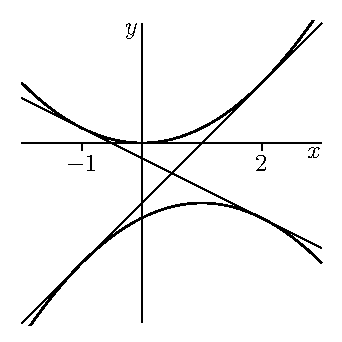
\includegraphics{graphE3c}
\end{center}
$y=4x-4$ and $y=-2x-1$
\end{answer}
\begin{solution}
The line $y=mx+b$ is tangent to $y=x^2$ at $x=\alpha$ if
$$
2\alpha=m\hbox{ and }\alpha^2=m\alpha+b
\iff m=2\alpha\hbox{ and }b=-\alpha^2
$$
The same line $y=mx+b$ is tangent to $y=-x^2+2x-5$ at $x=\beta$ if
\begin{align*}
-2\beta+2=m&\hbox{ and }-\beta^2+2\beta-5=m\beta+b\\
\iff m=2-2\beta&\hbox{ and }b=-\beta^2+2\beta-5-(2-2\beta)\beta=\beta^2-5
\end{align*}
For the line to be simultaneously tangent to the two parabolas we need
$$
m=2\alpha=2-2\beta\hbox{ and }b=-\alpha^2=\beta^2-5
$$
Substituting $\alpha=1-\beta$ into $-\alpha^2=\beta^2-5$ gives $-(1-\beta)^2=\beta^2-5$
or $2\beta^2-2\beta-4=0$ or $\beta=-1,2$. The corresponding values of the other
parameters are $\alpha=2,-1$, $m=4,-2$ and $b=-4,-1$. The two lines are
{$y=4x-4$ and $y=-2x-1$}.
\begin{center}
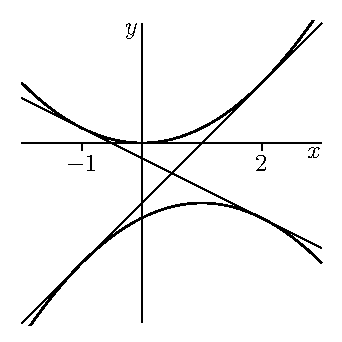
\includegraphics{graphE3c}
\end{center}
\end{solution}


\begin{question}[2015Q]
 Evaluate $\displaystyle \lim_{x\to 2015}\left(
\dfrac{\cos(x)-\cos(2015)}{x-2015}\right).$
\end{question}
\begin{hint}
Compare this to one of the forms given in the text for the definition of the derivative.
\end{hint}
\begin{answer}
{$-\sin(2015)$}
\end{answer}
\begin{solution}
This limit represents the derivative computed at $x=2015$ of the function
$f(x)=\cos(x)$. To see this, simply use the definition of the derivative at $a=2015$ with $f(x)=\cos x$:
\begin{align*}
\left.\diff{}{x}\{f(x)\}\right|_{a} &= \lim_{x \to a}\frac{f(x)-f(a)}{x-a}\\
\left.\diff{}{x}\{\cos x\}\right|_{2015} &= \lim_{x\to2015}\frac{\cos(x)-\cos(2015)}{x-2015}
\end{align*}
Since the derivative of $f(x)$ is $-\sin(x)$, its value at
$x=2015$ is exactly $-\sin(2015)$.
\end{solution}




\begin{question}[2015Q]
Evaluate $\displaystyle \lim_{x\to \pi/3}\left(
\dfrac{\cos(x)-1/2}{x-\pi/3}\right).$
\end{question}
\begin{hint}
Compare this to one of the forms given in the text for the definition of the derivative.
\end{hint}
\begin{answer}
{$-\sqrt{3}/2$}
\end{answer}
\begin{solution}
This limit represents the derivative computed at $x=\pi/3$ of the function
$f(x)=\cos x$. To see this, simply use the definition of the derivative at $a=\pi/3$ with $f(x)=\cos x$:
\begin{align*}
\left.\diff{}{x}\{f(x)\}\right|_{a} &= \lim_{x \to a}\frac{f(x)-f(a)}{x-a}\\
\left.\diff{}{x}\{\cos x\}\right|_{\pi/3} &= \lim_{x\to\pi/3}\frac{\cos(x)-\cos(\pi/3)}{x-\pi/3}\\
&=\lim_{x\to\pi/3} \frac{\cos(x)-1/2}{x-\pi/3}
\end{align*}
Since the derivative of $f(x)$ is $-\sin x$, then its
value at $x=\pi/3$ is exactly\\ $-\sin(\pi/3)=-\sqrt{3}/2$.
\end{solution}



\begin{question}[2015Q]
Evaluate $\displaystyle \lim_{x\to \pi}\left(\dfrac{\sin(x)}{x-\pi}\right).$
\end{question}
\begin{hint}
Compare this to one of the forms given in the text for the definition of the derivative.
\end{hint}
\begin{answer} $-1$
\end{answer}
\begin{solution}
    This limit represents the derivative computed at $x=\pi$ of the function $f(x)=\sin(x)$.
    To see this, simply use the definition of the derivative at $a=\pi$ with $f(x)=\sin x$:
\begin{align*}
\left.\diff{}{x}\{f(x)\}\right|_{a} &= \lim_{x \to a}\frac{f(x)-f(a)}{x-a}\\
\left.\diff{}{x}\{\sin x\}\right|_{\pi} &=\lim_{x\to\pi} \frac{\sin(x)-\sin(\pi)}{x-\pi}\\
 &=\lim_{x\to\pi} \frac{\sin(x)}{x-\pi}
\end{align*}
    Since the derivative of $f(x)$ is $\cos(x)$, then its value at $x=\pi$ is exactly\\
     $\cos(\pi)=-1$.
\end{solution}





\begin{question}[2015Q]
Evaluate $\displaystyle \lim_{x\to 2}\left(
\dfrac{x^{2015}-2^{2015}}{x-2}\right).$
\end{question}
\begin{hint}
Compare this to one of the forms given in the text for the definition of the derivative.
\end{hint}
\begin{answer}
{$2015\cdot 2^{2014}$}
\end{answer}
\begin{solution}
This limit represents the derivative computed at $x=2$ of the function $f(x)=x^{2015}$.
To see this, simply use the definition of the derivative at $a=2$ with $f(x)=x^{2015}$:
\begin{align*}
\left.\diff{}{x}\{f(x)\}\right|_{a} &= \lim_{x \to a}\frac{f(x)-f(a)}{x-a}\\
\left.\diff{}{x}\{x^{2015}\}\right|_{2} &=\lim_{x\to2} \frac{x^{2015}-2^{2015}}{x-2}
\end{align*}
Since the derivative of $f(x)$ is $2015\cdot x^{2014}$, then its value at $x=2$ is exactly $2015\cdot 2^{2014}$.
\end{solution}

\section{Derivatives of Exponential Functions}
%
% Copyright 2018 Joel Feldman, Andrew Rechnitzer and Elyse Yeager.
% This work is licensed under a Creative Commons Attribution-NonCommercial-ShareAlike 4.0 International License.
% https://creativecommons.org/licenses/by-nc-sa/4.0/
%
\questionheader{ex:s2.7}%
%%%%%%%%%%%%%%%%%%
\subsection*{\Conceptual}
%%%%%%%%%%%%%%%%%%


\begin{Mquestion}
Match the curves in the graph to the following functions:
\[ (a)~ y=\left(\frac{1}{2}\right)^x \qquad(b)~ y=1^x\qquad (c)~ y=2^x  \qquad (d)~ y=2^{-x}\qquad(e)~ y=3^x  \]
\begin{center}
\begin{tikzpicture}
\YEaaxis{5}{5}{1}{5}
\draw[thick] plot[domain=-5:5](\x,1)node[right]{D};%1
\draw[thick, red] plot[domain=-5:2.3](\x,{exp(\x*0.693)})node[above]{C};%2^x
\draw[thick, green] plot[domain=-2.3:5](\x,{1/exp(\x*0.693)});%.5^x
\draw[thick, green] (-2.3,5) node[above]{A};
\draw[thick, blue] plot[domain=-5:1.46](\x,{exp(\x*1.1)})node[above]{B};%3^x
\end{tikzpicture}
\end{center}
\end{Mquestion}
\begin{hint} Two of the functions are the same.
\end{hint}
\begin{answer} A-$(a)$ and $(d)$,\quad B-$(e)$,\quad C-$(c)$,\quad D-$(b)$
\end{answer}
\begin{solution} Since $1^x=1$ for any $x$, we see that $(b)$ is just the constant function $y=1$, so D matches to $(b)$.

Since $2^{-x}=\frac{1}{2^x}=\left(\frac{1}{2}\right)^x$, functions $(a)$ and $(d)$ are the same. This is the only function out of the lot that grows as $x\to-\infty$ and shrinks as $x \to \infty$, so A matches to $(a)$ and $(d)$.

This leaves B and C to match to $(c)$ and $(e)$. Since $3>2$, when $x>0$, $3^x>2^x$. So, $(e)$ matches to the function that grows more quickly to the right of the $x$-axis: B matches to $(e)$, and C matches to $(c)$.
\end{solution}

\begin{Mquestion}
The graph below shows an exponential function $f(x)=a^x$  and its derivative $f'(x)$. Choose all the options that describe the  constant $a$.
\[(a)~a<0\qquad(b)~a>0\qquad\qquad(c)~a<1\qquad(d)~a>1\qquad\qquad(e)~a<e\qquad(f)~a>e\]

\begin{center}
\begin{tikzpicture}
\YEaaxis{5}{5}{1}{5}
\draw[thick, blue] plot[domain=-5:3.97](\x,{exp(\x*0.405)})node[above]{$y=f(x)$};%1.5^x
\draw[thick, red] plot[domain=-5:5](\x,{0.405*exp(\x*0.405)})node[above]{$y=f'(x)$};%1.5^x
\end{tikzpicture}
\end{center}
\end{Mquestion}
\begin{hint}\end{hint}
\begin{answer} $(b),~(d),~(e)$
\end{answer}
\begin{solution}
First, let's consider the behaviour of exponential functions $a^x$ based on whether $a$ is greater or less than 1. As we know,
$\ds\lim_{x\to\infty}a^x=\left\{\begin{array}{ll}
\infty & a>1\\0&a<1
\end{array}\right.$ and $\ds\lim_{x\to-\infty}a^x=\left\{\begin{array}{ll}
0 & a>1\\\infty&a<1
\end{array}\right.$. Our function has $\ds\lim_{x \to \infty} f(x)=\infty$ and
$\ds\lim_{x \to -\infty} f(x)=0$, so we conclude $a>1$: thus $(d)$ and also $(b)$ hold. (We could have also seen that $(b)$ holds because $a^x$ is defined for all real numbers.)

It remains to decide whether $a$ is greater or less than $e$. (If $a$ were equal to $e$, then $f'(x)$ would be the same as $f(x)$.)  We saw in the text that $\diff{}{x}\{a^x\}=C(a)a^x$ for the function $C(a)=\ds\lim_{h \to 0} \dfrac{a^h-1}{h}$. We know that $C(e)=1$. (Actually, we chose $e$ to be the number that has this property.) From our graph, we see that $f'(x)<f(x)$, so $C(a)<1=C(e)$. In other words, $\ds\lim_{h \to 0} \dfrac{a^h-1}{h}<\ds\lim_{h \to 0} \dfrac{e^h-1}{h}$; so, $a<e$. Thus $(e)$ holds.
\end{solution}


\begin{question}
True or false: $\ds\diff{}{x}\{e^x\}=xe^{x-1}$
\end{question}
\begin{hint}
When can you use the power rule?
\end{hint}
\begin{answer}
False
\end{answer}
\begin{solution}
The power rule tells us that $\diff{}{x}\{x^n\}=nx^{n-1}$. In this equation, the variable is the base, and the exponent is a constant. In the function $e^x$, it's reversed: the variable is the exponent, and the base it a constant. So, the power rule does not apply.
\end{solution}



\begin{question}
A population of bacteria is described by $P(t)=100e^{0.2t}$, for $0 \leq t \leq 10$. Over this time period, is the population increasing or decreasing?

\medskip
We will learn more about the uses of exponential functions to describe real-world phenomena in Section~\ref*{sec:ExpGthDecay}.
\end{question}
\begin{hint} What is the shape of the curve $e^{ax}$, when $a$ is a positive consant?
\end{hint}
\begin{answer} increasing
\end{answer}
\begin{solution}
$P(t)$ is an increasing function over its domain, so the population is increasing.

There are a few ways to see that $P(t)$ is increasing.

 What we really care about is whether $e^{0.2t}$ is increasing or decreasing, since an increasing function multiplied by 100 is still an increasing function, and a decreasing function multiplied by 100 is still a decreasing function. Since $f(t)=e^t$ is an increasing function, we can use what we know about graphing functions to see that $f(0.2t)=e^{0.2t}$ is also increasing.
\end{solution}


%%%%%%%%%%%%%%%%%%
\subsection*{\Procedural}
%%%%%%%%%%%%%%%%%%

\begin{question}
Find the derivative of $f(x)=\dfrac{e^{x}}{2x}$
.\end{question}
\begin{hint}
Quotient rule
\end{hint}
\begin{answer}
$\dfrac{(x-1)e^x}{2x^2}$
\end{answer}
\begin{solution}
Using the quotient rule,
\begin{align*}
f'(x)=\frac{2xe^x-2e^x}{4x^2}=\frac{e^x(2x-2)}{4x^2}=\frac{(x-1)e^x}{2x^2}
\end{align*}
\end{solution}

\begin{question}\label{s2.7e2x}
Differentiate $f(x)=e^{2x}$.
\end{question}
\begin{hint}
$e^{2x}=\left(e^x\right)^2$
\end{hint}
\begin{answer}
$2e^{2x}$
\end{answer}
\begin{solution}
\begin{align*}
f'(x)=\diff{}{x}\{e^{2x}\}=\diff{}{x}\{(e^x)^2\}=2\diff{}{x}\{e^x\}e^x=2e^xe^x=2(e^{x})^2=2e^{2x}
\end{align*}
\end{solution}

\begin{question}
Differentiate $f(x)=e^{a+x}$, where $a$ is a constant.
\end{question}
\begin{hint}
$e^{a+x}=e^ae^x$
\end{hint}
\begin{answer}
$e^{a+x}$
\end{answer}
\begin{solution}
\begin{align*}
e^{a+x}&=e^ae^x
\intertext{Since $e^a$ is just a constant,}
\diff{}{x}\{e^{a}e^{x}\}&=e^a\diff{}{x}\{e^x\}=e^ae^x=e^{a+x}
\end{align*}
So, $f'(x)=f(x)=e^{a+x}$.
\end{solution}


\begin{question}
For which values of $x$ is the function $f(x)=xe^x$ increasing?
\end{question}
\begin{hint}
Figure out where the derivative is positive.
\end{hint}
\begin{answer}
$x>-1$
\end{answer}
\begin{solution}
If the derivative is positive, the function is increasing, so let's start by finding the derivative. We use the product rule (although Question~\ref{s2.7expprod} gives a shortcut).
\begin{align*}
f'(x)&=1\cdot e^x+xe^x=(1+x)e^x
\end{align*}
Since $e^x$ is always positive, $f'(x)>0$ when $1+x>0$. So, $f(x)$ is increasing when $x>-1$.
\end{solution}



\begin{Mquestion}
Differentiate $e^{-x}$.
\end{Mquestion}
\begin{hint}
$e^{-x}=\frac{1}{e^x}$
\end{hint}
\begin{answer}
$-e^{-x}$
\end{answer}
\begin{solution}
\begin{align*}e^{-x}&=\frac{1}{e^x}
\intertext{Using the rule for differentiating the reciprocal:}
\diff{}{x}\{e^{-x}\}&=\frac{-e^x}{(e^x)^2}=\frac{-1}{e^x}=-e^{-x}
\end{align*}
\end{solution}

\begin{question}
Differentiate $f(x)=(e^x+1)(e^x-1)$.
\end{question}
\begin{hint}
Product rule will work nicely here. Alternately, review the result of Question~\ref{s2.7e2x}.
\end{hint}
\begin{answer}
$2e^{2x}$
\end{answer}
\begin{solution}
Using the product rule,
\[f'(x)=(e^x)(e^x-1)+(e^x+1)(e^x)=e^x(e^x-1+e^x+1)=2(e^x)^2=2e^{2x}\]

Alternate solution: using Question~\ref{s2.7e2x}:
\[f(x)=e^{2x}-1 \implies f'(x)=2e^{2x}.\]
\end{solution}


\begin{Mquestion}
A particle's position  is given by
\[s(t)=t^2e^t.\]
 When is the particle moving in the negative direction?
\end{Mquestion}
\begin{hint}
To find the sign of a product, compare the signs of each factor. The function $e^t$ is always positive.
\end{hint}
\begin{answer}
When $t$ is in the interval $(-2,0)$.
\end{answer}
\begin{solution}
The question asks when $s'(t)$ is negative. So, we start by differentiating. Using the product rule:
\begin{align*}
s'(t)&=e^t(t^2+2t)\\
&=e^t \cdot t(t+2)
\end{align*}
$e^t$ is always positive, so $s'(t)$ is negative when $t$ and $2+t$ have opposite signs. This occurs when $-2<t<0$.
\end{solution}


%%%%%%%%%%%%%%%%%%
\subsection*{\Application}
%%%%%%%%%%%%%%%%%%

\begin{Mquestion}\label{s2.7expprod}
Let  $g(x)=f(x)e^x$, for a differentiable function $f(x)$. Give a simplified formula for $g'(x)$.


Functions of the form $g(x)$ are relatively common. If you remember this formula, you can save yourself some time when you need to differentiate them. We will explore this more in Question~\ref{s2.14expprod}, Section~\ref*{sec higher diff}.%2.14
\end{Mquestion}
\begin{hint}
After you differentiate, factor out $e^x$.
\end{hint}
\begin{answer}
$g'(x)=[f(x)+f'(x)]e^x$
\end{answer}
\begin{solution}
Using the product rule,
$g'(x)=f'(x)e^x+f(x)e^x=[f(x)+f'(x)]e^x$
\end{solution}


\begin{Mquestion}
Which of the following functions describe a straight line?
\[(a) ~y=e^{3\log x}+1 \qquad (b) ~2y+5=e^{3+\log x} \qquad (c)~y=e^{2x}+4\qquad (d)~y=e^{\log x}3^e+\log 2\]
\end{Mquestion}
\begin{hint}
Simplify
\end{hint}
\begin{answer}
(b) and (d)
\end{answer}
\begin{solution}
We simplify the functions to get a better idea of what's going on.

($a$): $y=e^{3\log x}+1=\left(e^{\log x}\right)^3+1=x^3+1$. This is not a line.
\smallskip

($b$): $2y+5=e^{3+\log x}=e^3e^{\log x}=e^3x$. Since $e^3$ is a constant, $2y+5=e^3x$ is a line.
\smallskip

($c$): There isn't a fancy simplification here--this isn't a line. If that isn't a satisfactory answer, we can check: a line is a function with a constant slope. For our function,
$y'=\diff{}{x}\{e^{2x} +4\}=\diff{}{x}\{e^{2x}\}=\diff{}{x}\left\{(e^x)^2\right\}=2e^xe^x=2e^{2x}$. Since the derivative isn't constant, the function isn't a line.
\smallskip

($d$): $y=e^{\log x}3^e+\log 2=3^e\,x+\log 2$. Since $3^e$ and $\log 2$ are constants, this is a line.
\end{solution}


\begin{question}[2009H]
Find constants $a$, $b$ so that the following function is differentiable:
\[
f(x) =\left\{\begin{array}{ll}
ax^2 + b & x \le 1\\
e^x     &  x > 1\end{array}\right.
\]
\end{question}
\begin{hint}
In order to be differentiable, a function should be continuous. To determine the differentiability of the function at $x=1$, use the definition of the derivative.
\end{hint}
\begin{answer}
$a=b=\dfrac{e}{2}$
\end{answer}
\begin{solution}
When we say a function is differentiable without specifying a range, we mean that it is differentiable over its domain. The function $f(x)$ is differentiable when $x \neq 1$ for any values of $a$ and $b$; it is up to us to figure out which constants make it differentiable when $x=1$.

In order to be differentiable, a function must be continuous. The definition of continuity tells us that, for $f$ to be continuous at $x=1$, we need $\ds\lim_{x \to 1}f(x)=f(1)$. From the definition of $f$, we see $f(1)=a+b=\ds\lim_{x \to 1^-}f(x)$, so we need $\ds\lim_{x\to 1^+}f(x)=a+b$. Since $\ds\lim_{x \to 1^+}f(x)=e^1=e$, we specifically need
\[e=a+b.\]

Now, let's consider differentiability of $f$ at $x=1$. We need the following limit to exist:
\begin{align*}
\lim_{h \to 0} \frac{f(1+h)-f(1)}{h}&
\intertext{In particular, we need the one-sided limits to exist and be equal:}
\textcolor{red}{\lim_{h \to 0^-}\frac{f(1+h)-f(1)}{h}}&=\textcolor{blue}{\lim_{h \to 0^+}\frac{f(1+h)-f(1)}{h}}
\intertext{If $h<0$, then $1+h<1$, so $f(1+h)=a(1+h)^2+b$. If $h>0$, then $1+h>1$, so $f(1+h)=e^{1+h}$. With this in mind, we begin to evaluate the one-sided limits:}
\color{red}\lim_{h \to 0^-}\frac{f(1+h)-f(1)}{h}&\color{red}=
\lim_{h \to 0^-}\frac{[a(1+h)^2+b]-[a+b]}{h}\\
&\color{red}=\lim_{h \to 0^-}\frac{ah^2+2ah}{h}=2a\\
\color{blue}\lim_{h \to 0^+}\frac{f(1+h)-f(1)}{h}&\color{blue}=
\lim_{h \to 0^+}\frac{e^{1+h}-(a+b)}{h}
\intertext{Since we take $a+b$ to be equal to $e$ (to ensure continuity):}
&\color{blue}=
\lim_{h \to 0^+}\frac{e^{1+h}-e^1}{h}\\
&\color{blue}=\left.\diff{}{x}\{e^x\}\right|_{x=1}=e^1=e
\end{align*}

So, we also need
\[\textcolor{red}{2a}=\textcolor{blue}{e}\]

Therefore, the values of $a$ and $b$ that make $f$ differentiable are $a=b=\dfrac{e}{2}$.

%In order for $f$ to be differentiable at $x=1$, it must also
%be continuous at $x=1$. This forces $e^x\big|_{x=1}=\big[ax^2+b\big]_{x=1}$
%or $a+b=e$. In order for $f$ to be differentiable at $x=1$, the right hand
%derivative of $ax^2+b$ at $x=1$, which is $2ax\big|_{x=1}=2a$, must be
%the same as the left hand derivative of $e^x$ at $x=1$, which is
%$e^x\big|_{x=1}=e$. So we need
%$$
%a+b=e,\ 2a=e\implies a=b=\frac{e}{2}
%$$
\end{solution}

\section{Derivatives of trigonometric functions}
%
% Copyright 2018 Joel Feldman, Andrew Rechnitzer and Elyse Yeager.
% This work is licensed under a Creative Commons Attribution-NonCommercial-ShareAlike 4.0 International License.
% https://creativecommons.org/licenses/by-nc-sa/4.0/
%
\questionheader{ex:s2.8}

%%%%%%%%%%%%%%%%%%
\subsection*{\Conceptual}
%%%%%%%%%%%%%%%%%%

\begin{Mquestion}
Graph sine and cosine on the same axes, from $x=-2\pi$ to $x=2\pi$. Mark the points where $\sin x$ has a horizontal tangent. What do these points correspond to, on the graph of cosine?
\end{Mquestion}
\begin{hint}
A horizontal tangent line is where the graph appears to ``level off."
\end{hint}
\begin{answer}
\begin{center}\begin{tikzpicture}
\YEaxis{7}{1.2}
\draw (3.1,.2)--(3.1,-.2) node[below]{$\pi$};
\draw (-3.1,.2)--(-3.1,-.2) node[below]{$-\pi$};
\draw[thick, blue] plot[domain=-6.28:0](\x,{sin \x r});
\draw[thick, blue] plot[domain=-6.28:0](\x+6.28,{sin \x r}) node[above]{$y=\sin x$};
\foreach \x in {-4.71,1.57}
	{\draw[blue] ( \x,1) node[vertex]{};
	\draw[blue, dashed] (\x-.75,1)--(\x+.75,1);}
\foreach \x in {4.71,-1.57}
	{\draw[blue] ( \x,-1) node[vertex]{};
	\draw[blue, dashed] (\x-.75,-1)--(\x+.75,-1);}
\draw[thick, red] plot[domain=-6.28:0](\x,{cos \x r});
\draw[thick, red] plot[domain=-6.28:0](\x+6.28,{cos \x r}) node[above]{$y=\cos x$};
\foreach \x in {-4.71,4.71,1.57,-1.57}
	{\draw[red] (\x,0) node[vertex]{};}
\end{tikzpicture}\end{center}
The graph $f(x)=\sin x$ has horizontal tangent lines precisely at those points where $\cos x=0$.
\end{answer}
\begin{solution}
\begin{center}\begin{tikzpicture}
\YEaxis{7}{1.2}
\draw (3.1,.2)--(3.1,-.2) node[below]{$\pi$};
\draw (-3.1,.2)--(-3.1,-.2) node[below]{$-\pi$};
\draw[thick, blue] plot[domain=-6.28:0](\x,{sin \x r});
\draw[thick, blue] plot[domain=-6.28:0](\x+6.28,{sin \x r}) node[above]{$y=\sin x$};
\foreach \x in {-4.71,1.57}
	{\draw[blue] ( \x,1) node[vertex]{};
	\draw[blue, dashed] (\x-.75,1)--(\x+.75,1);}
\foreach \x in {4.71,-1.57}
	{\draw[blue] ( \x,-1) node[vertex]{};
	\draw[blue, dashed] (\x-.75,-1)--(\x+.75,-1);}
\draw[thick, red] plot[domain=-6.28:0](\x,{cos \x r});
\draw[thick, red] plot[domain=-6.28:0](\x+6.28,{cos \x r}) node[above]{$y=\cos x$};
\foreach \x in {-4.71,4.71,1.57,-1.57}
	{\draw[red] (\x,0) node[vertex]{};}
\end{tikzpicture}\end{center}
The graph $f(x)=\sin x$ has horizontal tangent lines precisely at those points where $\cos x=0$. This must be true, since $\diff{}{x}\{\sin x\}=\cos x$: where the derivative of sine is zero, cosine itself is zero.
\end{solution}

\begin{Mquestion}
Graph sine and cosine on the same axes, from $x=-2\pi$ to $x=2\pi$. Mark the points where $\sin x$ has a tangent line of maximum (positive) slope. What do these points correspond to, on the graph of cosine?
\end{Mquestion}
\begin{hint}
You are going to mark there points on the sine graph where the graph is the steepest, going up.
\end{hint}
\begin{answer}
\begin{center}\begin{tikzpicture}
\YEaxis{7}{1.2}
\draw (3.1,.2)--(3.1,-.2) node[below]{$\pi$};
\draw (-3.1,.2)--(-3.1,-.2) node[below]{$-\pi$};
\draw[thick, blue] plot[domain=-6.28:0](\x,{sin \x r});
\draw[thick, blue] plot[domain=-6.28:0](\x+6.28,{sin \x r}) node[above]{$y=\sin x$};
\foreach \x in {-6.28,0,6.28}
	{\draw[blue] ( \x,0) node[vertex]{};
	\draw[blue, dashed] (\x-1,-1)--(\x+1,1);}
\draw[thick, red] plot[domain=-6.28:0](\x,{cos \x r});
\draw[thick, red] plot[domain=-6.28:0](\x+6.28,{cos \x r}) node[above]{$y=\cos x$};
\foreach \x in {-6.28,0,6.28}
	{\draw[red] (\x,1) node[vertex]{};}
\end{tikzpicture}\end{center}
The graph $f(x)=\sin x$ has maximum slope at those points where $\cos x$ has a maximum. That is, where $\cos x = 1$.
\end{answer}
\begin{solution}
\begin{center}\begin{tikzpicture}
\YEaxis{7}{1.2}
\draw (3.1,.2)--(3.1,-.2) node[below]{$\pi$};
\draw (-3.1,.2)--(-3.1,-.2) node[below]{$-\pi$};
\draw[thick, blue] plot[domain=-6.28:0](\x,{sin \x r});
\draw[thick, blue] plot[domain=-6.28:0](\x+6.28,{sin \x r}) node[above]{$y=\sin x$};
\foreach \x in {-6.28,0,6.28}
	{\draw[blue] ( \x,0) node[vertex]{};
	\draw[blue, dashed] (\x-1,-1)--(\x+1,1);}
\draw[thick, red] plot[domain=-6.28:0](\x,{cos \x r});
\draw[thick, red] plot[domain=-6.28:0](\x+6.28,{cos \x r}) node[above]{$y=\cos x$};
\foreach \x in {-6.28,0,6.28}
	{\draw[red] (\x,1) node[vertex]{};}
\end{tikzpicture}\end{center}
The graph $f(x)=\sin x$ has maximum slope at those points where $\cos x$ has a maximum. This makes sense, because $f'(x)=\cos x$: the maximum values of the slope of sine correspond to the maximum values of cosine.
\end{solution}

%%%%%%%%%%%%%%%%%%
\subsection*{\Procedural}
%%%%%%%%%%%%%%%%%%


\begin{question}
Differentiate $f(x)=\sin x + \cos x +\tan x$.
\end{question}
\begin{hint}
You need to memorize the derivatives of sine, cosine, and tangent.
\end{hint}
\begin{answer}
$f'(x)=\cos x - \sin x + \sec^2 x$
\end{answer}
\begin{solution}
You should memorize the derivatives of sine, cosine, and tangent.\\
$f'(x)=\cos x - \sin x + \sec^2 x$
\end{solution}


\begin{Mquestion}
For which values of $x$ does the function $f(x)=\sin x + \cos x$ have a horizontal tangent?
\end{Mquestion}
\begin{hint}
There are infinitely many values. You need to describe them all.
\end{hint}
\begin{answer}
$x=\frac{\pi}{4}+\pi n$, for any integer $n$.
\end{answer}
\begin{solution}
$f'(x)=\cos x - \sin x$, so $f'(x)=0$ precisely when $\sin x = \cos x$. This happens at $\pi/4$, but it also happens at $5\pi/4$. By looking at the unit circle, it is clear that $\sin x = \cos x$ whenever $x = \frac{\pi}{4}+\pi n$ for some integer $n$.
\begin{center}
\begin{tikzpicture}
\YEaxis{2.75}{2.75}
\draw[thick] node[shape=circle, minimum size=4cm, draw, inner sep=0]{};
\draw[dashed] (-2.75,-2.75)--(2.75,2.75);
\draw (1.41,1.41) node[vertex, label=right:{$\sin (\pi/4) = \cos (\pi/4)$}]{};
\draw (-1.41,-1.41) node[vertex, label=left:{$\sin (5\pi/4) = \cos (5\pi/4)$}]{};
\end{tikzpicture}
\end{center}
\end{solution}


\begin{Mquestion}
Differentiate $f(x)=\sin^2 x + \cos^2 x$.
\end{Mquestion}
\begin{hint}
Simplify first.
\end{hint}
\begin{answer}
0
\end{answer}
\begin{solution}
\begin{itemize}
\item Solution 1: $f(x)=\sin^2x+\cos^2x=1$, so $f'(x)=\diff{}{x}\{1\}=0$.
\item Solution 2: Using the formula for the derivative of a squared function,
\begin{align*}
f'(x)=2\sin x \cos x + 2\cos x(- \sin x)=2\sin x \cos x - 2 \sin x \cos x =0.
\end{align*}
\end{itemize}
\end{solution}


\begin{question}
Differentiate $f(x)=2\sin x \cos x$.
\end{question}
\begin{hint}
The identity won't help you.
\end{hint}
\begin{answer}
$f'(x)=2(\cos^2 x - \sin ^2 x)$
\end{answer}
\begin{solution}
It is true that $2\sin x \cos x = \sin (2x)$, but we don't know the derivative of $\sin(2x)$. So, we use the product rule: \[f'(x)=2\cos x \cos x+2\sin x (-\sin x)=2(\cos^2 x - \sin ^2 x).\]
\end{solution}


\begin{question}
Differentiate $f(x)=e^x\cot x$.
\end{question}
\begin{answer}
$f'(x)=e^x(\cot x - \csc^2 x)$
\end{answer}
\begin{solution}
\begin{itemize}
\item Solution 1:
 using the product rule,
\[f'(x)=e^x\cot x + e^x(-\csc^2 x)=e^x(\cot x - \csc^2 x).\]
\item Solution 2:
using the formula from Question~\ref{s2.7expprod}, Section~\ref*{sec exp func},
\[f'(x)=e^x(\cot x - \csc^2 x).\]
\end{itemize}
\end{solution}


\begin{Mquestion}
Differentiate $f(x) = \dfrac{2\sin x + 3 \tan x}{\cos x + \tan x}$
\end{Mquestion}
\begin{hint}
Quotient rule
\end{hint}
\begin{answer}
$f'(x)=\dfrac{2+3 \sec x + 2 \sin x -2\tan x \sec x+3\sin x \tan x }{(\cos x + \tan x)^2}$
\end{answer}
\begin{solution}
We use the quotient rule.
\begin{align*}
f'(x)&=\dfrac{(\cos x + \tan x)(2\cos x + 3 \sec^2 x)-(2\sin x+3\tan x)(-\sin x + \sec^2 x)}{(\cos x + \tan x)^2}\\
&=\frac{2\cos^2x+3\cos x \sec^2 x + 2 \cos x \tan x + 3 \tan x \sec^2 x}{(\cos x + \tan x)^2}\\
&~~~~
+\frac{2\sin^2x-2\sin x \sec^2x+3\sin x \tan x -3\tan x \sec^2 x}{(\cos x + \tan x)^2}\\
&=\frac{2+3 \sec x + 2 \sin x -2\tan x \sec x+3\sin x \tan x }{(\cos x + \tan x)^2}
\end{align*}
\end{solution}

\begin{Mquestion}
Differentiate $f(x) = \dfrac{5\sec x+1}{e^x}$.
\end{Mquestion}
\begin{answer}
$f'(x)=\dfrac{5\sec x \tan x - 5 \sec x - 1}{e^x}$
\end{answer}
\begin{solution}
We use the quotient rule.
\begin{align*}
f'(x) &= \frac{e^x(5\sec x \tan x)-(5\sec x + 1) e^x}{(e^{x})^2}\\
&=\frac{5\sec x \tan x - 5 \sec x - 1}{e^x}
\end{align*}
\end{solution}

\begin{question}
Differentiate $f(x)=(e^x+\cot x)(5x^6-\csc x)$.
\end{question}
\begin{answer}
$f'(x)=(e^x+\cot x)(30x^5+\csc x \cot x)+(e^x-\csc^2x)(5x^6-\csc x)$
\end{answer}
\begin{solution}
We use the product rule:
\begin{align*}
f'(x)&=(e^x+\cot x)(30x^5+\csc x \cot x)+(e^x-\csc^2x)(5x^6-\csc x)
\end{align*}
\end{solution}

\begin{question}
Differentiate $f(\theta)=\sin\left(\frac{\pi}{2}-\theta \right)$.
\end{question}
\begin{hint}
Use an identity.
\end{hint}
\begin{answer}
$-\sin(\theta)$
\end{answer}
\begin{solution}
We don't know how to differentiate this function as it is written, but an identity helps us.
Since $\sin\left(\frac{\pi}{2}-\theta \right)=\cos \theta$, we see
$f'(\theta)=\diff{}{\theta}\{\cos \theta\}=-\sin(\theta)$.
\end{solution}

\begin{question}
Differentiate $f(x)=\sin(-x)+\cos(-x)$.
\end{question}
\begin{hint}
How can you move the negative signs to a location that you can more easily deal with?
\end{hint}
\begin{answer}
$f'(x)=-\cos x - \sin x$
\end{answer}
\begin{solution}
We know the derivative of $\sin x$, but not of $\sin(-x)$. So we re-write $f(x)$ using identities:
\begin{align*}
f(x)&=\sin(-x)+\cos(-x)\\
&=-\sin x + \cos x\\
f'(x)&=-\cos x - \sin x
\end{align*}
\end{solution}


\begin{question}
Differentiate $s(\theta)=\dfrac{\cos \theta + \sin \theta}{\cos \theta - \sin\theta}$.
\end{question}
\begin{hint} Apply the quotient rule.
\end{hint}
\begin{answer}
$\left(\dfrac{\cos\theta+\sin\theta}{\cos\theta-\sin\theta}\right)^2+1$
\end{answer}
\begin{solution}
We apply the quotient rule.
\begin{align*}
s'(\theta)&=\frac{(\cos \theta-\sin\theta)(-\sin\theta+\cos\theta)-(\cos\theta+\sin\theta)(-\sin\theta-\cos\theta)}{(\cos\theta-\sin\theta)^2}\\
&=\frac{(\cos \theta-\sin\theta)^2+(\cos\theta+\sin\theta)^2}{(\cos\theta-\sin\theta)^2}\\
&=1+\left(\frac{\cos\theta+\sin\theta}{\cos\theta-\sin\theta}\right)^2
\end{align*}
\end{solution}


\begin{question}[2007H]
Find the values of the constants $a$ and $b$ for which
\[
f(x) = \left\{
	\begin{array}{cc} \cos(x) & x\le 0\\
               ax + b   &  x> 0\end{array}
               \right.
\]
is differentiable everywhere.
\end{question}
\begin{hint}
The only spot to worry about is when $x=0$. For $f(x)$ to be differentiable, it must be continuous, so first find the value of $b$ that makes $f$ continuous at $x=0$. Then, find the value of $a$ that makes the derivatives from the left and right of $x=0$ equal to each other.
\end{hint}
\begin{answer}
$a=0$, $b=1$.
\end{answer}
\begin{solution}
In order for $f$ to be differentiable at $x=0$, it must also
be continuous at $x=0$. This forces
\[
\lim_{x\to 0^-}f(x) =  \lim_{x\to 0^+}f(x) =f(0)\qquad\text{or}\qquad
\lim_{x\to 0^-}\cos(x) =  \lim_{x\to 0^+}(ax+b) =1
\]
or $b=1$. In order for $f$ to be differentiable at $x=0$, we need the limit
\[
\lim_{h\to 0}\frac{f(0+h)-f(0)}{h}
\]
to exist. This is the case if and only if the two one--sided limits
\begin{align*}
\lim_{h\to 0^-}\frac{f(0+h)-f(0)}{h}
&=\lim_{h\to 0^-}\frac{\cos(h)-\cos(0)}{h}
\intertext{and}
\lim_{h\to 0^+}\frac{f(0+h)-f(0)}{h}
&=\lim_{h\to 0^+}\frac{(ah+b)-\cos(0)}{h}
=a\qquad\text{since $b=1$}
\intertext{exist and are equal.
Because $\cos(x)$ is differentiable at $x=0$ we have}
\lim_{h\to 0^-}\frac{\cos(h)-\cos(0)}{h} &= \diff{}{x}\cos(x)\bigg|_{x=0}
                                         = -\sin(x)\Big|_{x=0}=0
\end{align*}
So, we need $a=0$ and $b=1$.
\end{solution}




\begin{Mquestion}[2015Q]
Find the equation of the line tangent to the graph of $y=\cos(x)+2x$ at
$x=\dfrac{\pi}{2}$.
\end{Mquestion}
\begin{answer} $y -  \pi = 1\cdot (x-\pi/2)$
\end{answer}
\begin{solution}
We compute the derivative of $\cos(x)+2x$ as being $-\sin(x)+2$, which evaluated at
$x=\frac{\pi}{2}$ yields $-1+2=1$. Since we also compute
$\cos(\pi/2)+2(\pi/2)=0+\pi$, then the equation of the tangent line is
\begin{align*}
y -  \pi = 1\cdot (x-\pi/2).
\end{align*}
\end{solution}


%%%%%%%%%%%%%%%%%%
\subsection*{\Application}
%%%%%%%%%%%%%%%%%%

\begin{question}[2015Q]
 Evaluate $\displaystyle \lim_{x\to \pi/3}\left(
\dfrac{\cos(x)-1/2}{x-\pi/3}\right).$  Use any method.
\end{question}
\begin{hint} This looks like a derivative that you know how to compute.
\end{hint}
\begin{answer}  $-\sqrt{3}/2$
\end{answer}
\begin{solution}
This limit represents the derivative computed at $x=\pi/3$ of the function
$f(x)=\cos x$. Since the derivative of $f(x)$ is $-\sin x$, then its
value at $x=\pi/3$ is exactly $-\sqrt{3}/2$.
\end{solution}

\begin{question}
Show how you can use the quotient rule to find the derivative of tangent, if you already know the derivatives of sine and cosine.
\end{question}
\begin{hint}
$\tan \theta = \dfrac{\sin \theta}{\cos \theta}$
\end{hint}
\begin{answer}
\begin{align*}
\tan \theta &= \dfrac{\sin \theta}{\cos \theta}
\intertext{So, using the quotient rule,}
\diff{}{\theta}\{\tan \theta\}&=\frac{\cos\theta\cos\theta-\sin\theta(-\sin\theta)}{\cos^2\theta}
=\frac{\cos^2\theta+\sin^2\theta}{\cos^2\theta}\\
&=\left(\frac{1}{\cos \theta}\right)^2=\sec^2\theta
\end{align*}
\end{answer}
\begin{solution}
\begin{align*}
\tan \theta &= \dfrac{\sin \theta}{\cos \theta}
\intertext{So, using the quotient rule,}
\diff{}{\theta}\{\tan \theta\}&=\frac{\cos\theta\cos\theta-\sin\theta(-\sin\theta)}{\cos^2\theta}
=\frac{\cos^2\theta+\sin^2\theta}{\cos^2\theta}\\
&=\left(\frac{1}{\cos \theta}\right)^2=\sec^2\theta
\end{align*}
\end{solution}


\begin{question}[1997A]
 The derivative of the function
\[
f(x)=\left\{\begin{array}{ll}
ax+b& \mbox{for }x<0\\
            \frac{6\cos x}{2+\sin x+\cos x}& \mbox{for }x\ge 0
\end{array}\right.
\]
exists and is continuous for all $x$. Determine the values of the constants
$a$ and $b$.
\end{question}
\begin{hint} In order for a derivative to exist, the function must be continuous, and the derivative from the left must equal the derivative from the right.
\end{hint}
\begin{answer} $a=-\frac{2}{3}$, $b=2$
\end{answer}
\begin{solution}  In order for the function $f(x)$ to be continuous at $x=0$,
the left half formula $ax+b$ and the right half formula
$\dfrac{6\cos x}{2+\sin x+\cos x}$ must match up at $x=0$. This
forces
$$
a\times 0+b=\frac{6\cos 0}{2+\sin 0+\cos 0}=\frac{6}{3}
\implies \boxed{b=2}
$$

In order for the derivative $f'(x)$ to exist at $x=0$,
the limit $\ds\lim_{h \rightarrow 0} \dfrac{f(h)-f(0)}{h}$ must exist. In particular,
the limits $\ds\lim_{h \rightarrow 0^-} \dfrac{f(h)-f(0)}{h}$
and
$\ds\lim_{h \rightarrow 0^+} \dfrac{f(h)-f(0)}{h}$ must exist and be equal to each other.

When $h \to 0^-$, this means $h<0$, so $f(h)=ah+b=ah+2$. So:
\[\ds\lim_{h\to 0^-}\dfrac{f(h)-f(0)}{h}=\ds\lim_{h\to 0^-}\dfrac{(ah+2)-2}{h}=\left.\ds\diff{}{x}\left\{ax+2\right\}\right|_{x=0}=a.\]

Similarly, when $h \to 0^+$, then $h>0$, so $f(h)=\dfrac{6\cos h}{1+\sin h + \cos h}$ ~~and \begin{align*}
\ds\lim_{h \rightarrow 0^+} \dfrac{f(h)-f(0)}{h} &= \left.\ds\diff{}{x}\left\{\dfrac{6\cos x}{2+\sin x + \cos x}\right\}\right|_{x=0}
\\&=\left.\frac{-6\sin x(2+\sin x+\cos x)-6\cos x(\cos x-\sin x)}{(2+\sin x+\cos x)^2}\right|_{x=0}.\end{align*}

Since the limits from the left and right must be equal, this forces
$$
a=\frac{-6\sin 0(2+\sin 0+\cos 0)-6\cos 0(\cos 0-\sin 0)}{(2+\sin 0+\cos 0)^2}
=\frac{-6}{(2+1)^2}\implies\boxed{a=-\frac{2}{3}}
$$
\end{solution}


\begin{question}[2015Q]
For which values of $x$ does the derivative of $f(x) = \tan x$ exist?
\end{question}
\begin{hint}
There are infinitely many places where it does \emph{not} exist.
\end{hint}
\begin{answer}
All values of $x$ except $x=\frac{\pi}{2}+n\pi$, for any integer $n$.
\end{answer}
\begin{solution}
In order for $f'(x)$ to exist, $f(x)$ has to exist. We already know that $\tan x $ does not exist whenever $x=\frac{\pi}{2}+n\pi$ for any integer $n$. If we look a little deeper, since $\tan x = \frac{\sin x}{\cos x}$, the points where tangent does not exist correspond exactly to the points where cosine doesn't exist.

From its graph, tangent looks like a smooth curve over its domain, so we might guess that everywhere tangent is defined, its derivative is defined. We can check this: $f'(x) = \sec^2 x = \left(\frac{1}{\cos x}\right)^2$. Indeed, wherever $\cos x$ is nonzero, $f'$ exists.

So, $f'(x)$ exists for all values of $x$ \emph{except} when $x=\frac{\pi}{2}+n\pi$ for some integer $n$.
\end{solution}


\begin{Mquestion}[2015Q]
For what values of $x$ does the derivative of
$\dfrac{10\sin(x)}{x^2+x-6}$ exist? Explain your answer.
\end{Mquestion}
\begin{answer}
The function is differentiable whenever $x^2+x-6\ne 0$ since the derivative equals
\begin{align*}
\frac{10\cos(x)\cdot (x^2+x-6)-10\sin(x)\cdot (2x+1)}{(x^2+x-6)^2},
\end{align*}
which is well-defined unless $x^2+x-6=0$. We solve $x^2+x-6=(x-2)(x+3)=0,$
and get $x=2$ and $x=-3$. So, the function is differentiable for all real values $x$ except for $x=2$ and for $x=-3$.
\end{answer}
\begin{solution}
The function is differentiable whenever $x^2+x-6\ne 0$ since the derivative equals
\begin{align*}
\frac{10\cos(x)\cdot (x^2+x-6)-10\sin(x)\cdot (2x+1)}{(x^2+x-6)^2},
\end{align*}
which is well-defined unless $x^2+x-6=0$. We solve $x^2+x-6=(x-2)(x+3)=0,$
and get $x=2$ and $x=-3$. So, the function is differentiable for all real values $x$ except for $x=2$ and for $x=-3$.
\end{solution}



\begin{question}[test]
For what values of $x$ does the derivative of
$\dfrac{x^2+6x+5}{\sin(x)}$ exist? Explain your answer.
\end{question}
\begin{answer}
The function is differentiable whenever $\sin(x)\ne 0$ since the derivative equals
\begin{align*}
\frac{\sin(x)\cdot (2x+6) - \cos(x)\cdot (x^2+6x+5)}{(\sin x)^2},
\end{align*}
which is well-defined unless $\sin x = 0$. This happens when $x$ is an integer multiple
of $\pi$. So, the function is differentiable for all real values $x$ except $x=n\pi,$, where $n$ is any integer.
\end{answer}
\begin{solution}
The function is differentiable whenever $\sin(x)\ne 0$ since the derivative equals
\begin{align*}
\frac{\sin(x)\cdot (2x+6) - \cos(x)\cdot (x^2+6x+5)}{(\sin x)^2},
\end{align*}
which is well-defined unless $\sin x = 0$. This happens when $x$ is an integer multiple
of $\pi$. So, the function is differentiable for all real values $x$ except $x=n\pi,$, where $n$ is any integer.
\end{solution}


\begin{question}[2015Q]
 Find the equation of the line tangent to the graph of $y=\tan(x)$ at
$x=\dfrac{\pi}{4}$.
\end{question}
\begin{answer}
$y -  1 = 2\cdot (x-\pi/4)$
\end{answer}
\begin{solution}
We compute the derivative of $\tan(x)$ as being $\sec^2(x)$, which evaluated at
$x=\frac{\pi}{4}$ yields $2$. Since we also compute
$\tan(\pi/4)=1$, then the equation of the tangent line is
\begin{align*}
y -  1 = 2\cdot (x-\pi/4).
\end{align*}
\end{solution}


\begin{question}[2015Q]
Find the equation of the line tangent to the graph of $y=\sin(x)+\cos(x)+e^x$
at
$x=0$.
\end{question}
\begin{answer} $y=2x+2$
\end{answer}
\begin{solution}
We compute the derivative $y' = \cos(x)-\sin(x)+e^x$, which evaluated at
$x=0$ yields $1-0+1 = 2$. Since we also compute $y(0)=0+1+1=2$, the equation of the
tangent line is
\begin{align*}
y -  2 = 2(x-0)
\end{align*}
ie $y=2x+2$.
\end{solution}


\begin{question}
For which values of $x$ does the function $f(x)=e^x\sin x$ have a horizontal tangent line?
\end{question}
\begin{answer}
$x = \frac{3\pi}{4}+n\pi$ for any integer $n$.
\end{answer}
\begin{solution}
We are asked to solve $f'(x)=0$. That is, $e^x[\sin x +  \cos x]=0$. Since $e^x$ is always positive, that means we need to find all points where $\sin x + \cos x =0$. That is, we need to find all values of $x$ where $\sin x = - \cos x$. Looking at the unit circle, we see this happens whenever $x = \frac{3\pi}{4}+n\pi$ for any integer $n$.
\begin{center}
\begin{tikzpicture}
\YEaxis{2.75}{2.75}
\draw[thick] node[shape=circle, minimum size=4cm, draw, inner sep=0]{};
\draw[dashed] (2.75,-2.75)--(-2.75,2.75);
\draw (1.41,-1.41) node[vertex, label=right:{$\sin (-\pi/4) = -\cos (-\pi/4)$}]{};
\draw (-1.41,1.41) node[vertex, label=left:{$\sin (3\pi/4) = -\cos (3\pi/4)$}]{};
\end{tikzpicture}
\end{center}
\end{solution}

%%%
%%% Andrew - extra problem starts here
%%%

\begin{question}
Let
\[f(x)=\left\{\begin{array}{ccc}
\frac{\sin x}{x}&,&x \neq 0\\
1&,&x=0
\end{array}\right.\]
Find $f'(0)$, or show that it does not exist.
\end{question}
\begin{hint}
You can set up the derivative using the limit definition: $f'(0)=\ds\lim_{h \to 0}\dfrac{f(h)-f(0)}{h}$. If the limit exists, it gives you $f'(0)$; if the limit does not exist, you conclude $f'(0)$ does not exist.

To evaluate the limit, recall that when we differentiated sine, we learned that for $h$ near 0,
\[\cos h \leq \frac{\sin h}{h}\leq 1\]
\end{hint}
\begin{answer}
$f'(0)=0$
\end{answer}
\begin{solution}
First, we note that our function is continuous, because
\[\lim_{x \to 0} f(x)=\lim_{x \to 0} \frac{\sin x}{x}=1=f(0)\]
This is a handy thing to check: if the function were discontinuous at $x=0$, then we would automatically know that it was not differentiable there.

Now, on to the derivative. We can use the limit definition:
\begin{align*}
f'(0)&=\lim_{h \to 0}\frac{f(0+h)-f(0)}{h}\qquad\mbox{ if it exists}\\
&=\lim_{h \to 0} \frac{f(h)-1}{h}\\
&=\lim_{h \to 0} \frac{\frac{\sin h}{h}-1}{h}
\end{align*}
As $h$ approaches 0, both the numerator and the denominator approach 0. So, to evaluate the limit, we need to do more work. The key insight we can use is a result that was shown in the text while evaluating the derivative of sine. When $h$ is close to 0, $\cos h \leq \frac{\sin h}{h} \leq 1$. We use this to bound our limit, and then apply the squeeze theorem.
\begin{align*}
&\cos h&&\leq&&\frac{\sin h}{h}&&\leq&&1\\
\mbox{So, }\qquad&\frac{\cos h-1}{h}&&\leq&&\frac{\frac{\sin h}{h}-1}{h}&&\leq&&\frac{1-1}{h}=0
\end{align*}
We evaluate the limits of the bounds. For the lower bound, notice its similarity to the definition of the derivative.
\begin{align*}
\lim_{h \to 0}\frac{\cos h-1}{h}&=\lim_{h \to 0}\frac{\cos(0+h)-\cos(0)}{h}\\
&=\diff{}{x}\left.\left\{\cos x \right\}\right|_{x=0}=0\\
\lim_{h \to 0}0&=0
\end{align*}
So, by the Squeeze Theorem, $f'(0)=\ds\lim_{h \to 0}\frac{\frac{\sin h}{h}-1}{h}=0$.
\end{solution}

%%%
%%% Andrew - extra problem ends here
%%%


%%%%%%%%%%%%%%%%%%
\subsection*{Application of Understanding}
%%%%%%%%%%%%%%%%%%


\begin{question}[2010H]
Differentiate the function \[h(x) = \sin(|x|)\] and give the domain where the derivative exists.
\end{question}
\begin{hint}
Recall $|x|=\left\{\begin{array}{rl}
x&x\ge 0\\
-x&x<0
\end{array}\right.$. To determine whether $h(x)$ is differentiable at $x=0$, use the definition of the derivative.
\end{hint}
\begin{answer}
$h'(x)=\left\{\begin{array}{rl}
\cos x&x> 0\\
-\cos x&x<0
\end{array}\right.$ It exists for all $x \neq 0$.
\end{answer}
\begin{solution}
As usual, when dealing with the absolute value function, we can make things a little clearer by splitting it up into two pieces.
\begin{align*}
|x|&=\left\{\begin{array}{rl}
x&x\ge 0\\
-x&x<0
\end{array}\right.\intertext{So,}
\sin|x|&=\left\{\begin{array}{rl}
\sin x&x\ge 0\\
\sin(-x)&x<0
\end{array}\right.
=\left\{\begin{array}{rl}
\sin x&x\ge 0\\
-\sin x&x<0
\end{array}\right.
\intertext{where we used the identity $\sin(-x)=-\sin x$. From here, it's easy to see $h'(x)$ when $x$ is anything \emph{other than} zero.}
\diff{}{x}\{\sin|x|\}&=\left\{\begin{array}{rl}
\cos x&x> 0\\
??&x=0\\
-\cos x&x<0
\end{array}\right.
\intertext{To decide whether $h(x)$ is differentiable at $x=0$, we use the definition of the derivative. One word of explanation: usually in the definition of the derivative, $h$ is the tiny ``change in $x$" that is going to zero. Since $h$ is the name of our function, we need another letter to stand for the tiny change in $x$, the size of which is tending to zero. We chose $t$.}
\lim_{t \to 0} \frac{h(t+0)-h(0)}{t}&=\lim_{t \to 0}\frac{\sin|t|}{t}
\intertext{We consider the behaviour of this function to the left and right of $t=0$:}
\frac{\sin |t|}{t}&=\left\{\begin{array}{ll}
\frac{\sin t}{t} & t\ge 0\\
\frac{\sin (-t)}{t} & t <0
\end{array}\right.
=\left\{\begin{array}{ll}
\frac{\sin t}{t} & t\ge 0\\
-\frac{\sin t}{t} & t <0
\end{array}\right.
\intertext{Since we're evaluating the limit as $t$ goes to zero, we need the fact that $\ds\lim_{t \to 0}\dfrac{\sin t}{t}=1$.
We saw this in Section~\ref*{sec exp func}, but also we know enough now to evaluate it another way. Using the definition of the derivative: }
\lim_{t \to 0}\frac{\sin t}{t}&=\lim_{t \to 0}\frac{\sin (t+0)-\sin (0)}{t}=\left.\diff{}{x}\{\sin x\}\right|_{t=0}=\cos 0=1
\intertext{At any rate, since we know $\ds\lim_{t \to 0}\dfrac{\sin t}{t}=1$, then:}
\lim_{t \to 0^+} \frac{h(t+0)-h(0)}{t}&=\lim_{t \to 0^+}\frac{\sin t}{t}=1\qquad
\lim_{t \to 0^-} \frac{h(t+0)-h(0)}{t}=\lim_{t \to 0^-}\frac{-\sin t}{t}=-1
\intertext{So, since the one-sided limits disagree,}
\lim_{t \to 0} \frac{h(t+0)-h(0)}{t}&=DNE
\intertext{so $h(x)$ is not differentiable at $x=0$. Therefore,}
h'(x)&=\left\{\begin{array}{rl}
\cos x&x> 0\\
-\cos x&x<0
\end{array}\right.
\end{align*}

\end{solution}


\begin{Mquestion}[2006H]
For the function
\[
f(x) =\left\{\begin{array}{ll} 0 & x\le 0\\
               \frac{\sin(x)}{\sqrt{x}} & x > 0\end{array}\right.
\]

which of the following statements is correct?
\begin{enumerate}[i.]
\item\label{s2.8_2006i} $f$ is undefined at $x = 0$.
\item\label{s2.8_2006ii}  $f$ is neither continuous nor differentiable at $x = 0$.
\item\label{s2.8_2006iii}  $f$ is continuous but not differentiable at $x = 0$.
\item\label{s2.8_2006iv} $f$ is differentiable but not continuous at $x = 0$.
\item\label{s2.8_2006v} $f$ is both continuous and differentiable at $x = 0$.
\end{enumerate}
\end{Mquestion}
\begin{hint} To decide whether the function is differentiable, use the definition of the derivative.
\end{hint}
\begin{answer} \ref{s2.8_2006iii}
\end{answer}
\begin{solution}
Statement \ref{s2.8_2006i} is false, since $f(0)=0$.
Statement \ref{s2.8_2006iv} cannot hold, since a function that is differentiable is also continuous.

Since $\ds\lim_{x\rightarrow 0+}\frac{\sin x}{x}=1$ (we saw this in Section~\ref*{sec diff trig}%2.8
),
\begin{align*}
\lim_{x\rightarrow 0+}f(x)&=\lim_{x\rightarrow 0+}\frac{\sin x}{\sqrt{x}}\\
&=\lim_{x\rightarrow 0+}\sqrt{x}\frac{\sin x}{x}\\&=0\cdot 1=0
\intertext{So $f$ is continuous at $x=0$, and so
Statement \ref{s2.8_2006ii} does not hold. Now, let's consider $f'(x)$.}
\lim_{x\rightarrow 0+}\frac{f(x)-f(0)}{x}
&=\lim_{x\rightarrow 0+}\frac{\frac{\sin x}{\sqrt{x}}-0}{x}\\
&=\lim_{x\rightarrow 0+}\frac{1}{\sqrt{x}}\frac{\sin x}{x}=+\infty
\intertext{Therefore, using the definition of the derivative,}
f'(0)&=\lim_{x \to 0}\frac{f(x)-f(0)}{x}~~\mbox{ if it exists, but}\\
\lim_{x \to 0}\frac{f(x)-f(0)}{x}&=DNE
\end{align*}
since one of the one-sided limits does not exist. So $f$ is continuous but not differentiable
at $x=0$. The correct statement is \ref{s2.8_2006iii}.
\end{solution}





\begin{question}[2011H]
Evaluate $\lim\limits_{x\rightarrow 0}
                 \dfrac{\sin x^{27}+2x^5 e^{x^{99}}}{\sin^5 x}$.
\end{question}
\begin{hint}
In this chapter, we learned $\ds\lim_{x \to 0}\dfrac{\sin x}{x}=1$. If you divide the numerator and denominator by $x^5$, you can make use of this knowledge.
\end{hint}
\begin{answer} $2$
\end{answer}
\begin{solution}
Recall that $\lim\limits_{x\rightarrow 0}\dfrac{\sin x}{x} =1$. In order to take advantage of this knowledge, we divide the numerator and denominator by $x^5$ (because $5$ is the power of sine in the denominator, and a denominator that goes to zero generally makes a limit harder).
\begin{align*}
\lim_{x\rightarrow 0}  \dfrac{\sin x^{27}+2x^5 e^{x^{99}}}{\sin^5 x}
&=\lim_{x\rightarrow 0}  \dfrac{\dfrac{\sin x^{27}}{x^{5}}+2 e^{x^{99}}}
                                {\left(\dfrac{\sin x}{x}\right)^5}
\intertext{Now the denominator goes to 1, which is nice, but we need to take care of the fraction $\dfrac{\sin x^{27}}{x^5}$ in the numerator. This fraction isn't very familiar, but we know what happens to the fraction 
$\dfrac{\sin x^{27}}{x^{27}}=\left(\dfrac{\sin x}{x}\right)^{27}$:}
&=\lim_{x\rightarrow 0}  \dfrac{x^{22}\dfrac{\sin x^{27}}{x^{27}}+2 e^{x^{99}}}
                                {\left(\dfrac{\sin x}{x}\right)^5}
=\dfrac{0\times 1+2\times 1}{1^5}
=2
\end{align*}

\end{solution}

\section{One more tool - the chain rule}
%
% Copyright 2018 Joel Feldman, Andrew Rechnitzer and Elyse Yeager.
% This work is licensed under a Creative Commons Attribution-NonCommercial-ShareAlike 4.0 International License.
% https://creativecommons.org/licenses/by-nc-sa/4.0/
%
\questionheader{ex:s2.9}

%%%%%%%%%%%%%%%%%%
\subsection*{\Conceptual}
%%%%%%%%%%%%%%%%%%

\begin{Mquestion}
Suppose the amount of kelp in a harbour depends on the number of urchins. Urchins eat kelp: when there are more urchins, there is less kelp, and when there are fewer urchins, there is more kelp. Suppose further that the number of urchins in the harbour depends on the number of otters, who find urchins extremely tasty: the more otters there are, the fewer urchins there are.

Let $O$, $U$, and $K$ be the populations of otters, urchins, and kelp, respectively.
\begin{enumerate}[(a)]
\item\label{s2.9otter1} Is $\diff{K}{U}$ positive or negative?
\item\label{s2.9otter2} Is $\diff{U}{O}$ positive or negative?
\item\label{s2.9otter3} Is $\diff{K}{O}$ positive or negative?
\end{enumerate}
Remark: An urchin barren is an area where unchecked sea urchin grazing has decimated the kelp population, which in turn causes the other species that shelter in the kelp forests to leave. Introducing otters to urchin barrens is one intervention to increase biodiversity. A short video with a more complex view of otters and urchins in Canadian waters is available on YouTube: \url{https://youtu.be/ASJ82wyHisE}
\end{Mquestion}
\begin{hint}
For  parts~\eqref{s2.9otter1} and \eqref{s2.9otter2}, remember the definition of a derivative: \[\ds\diff{K}{U}=\ds\lim_{h \rightarrow 0}\dfrac{K(U+h)-K(U)}{h}.\] When $h$ is positive, $U+h$ is an increased urchin population; what is the sign of $K(U+h)-K(U)$?

For part~\eqref{s2.9otter3}, use the chain rule!
\end{hint}
\begin{answer}
\eqref{s2.9otter1} $\diff{K}{U}$ is negative\qquad
\eqref{s2.9otter2} $\diff{U}{O}$ is negative\qquad
\eqref{s2.9otter3} $\diff{K}{O}$ is positive
\end{answer}
\begin{solution}
\eqref{s2.9otter1}
More urchins means less kelp, and fewer urchins means more kelp. This means kelp and urchins are negatively correlated, so $\diff{K}{U}<0$.

If you aren't sure why that is, we give a more detailed explanation here, using the definition of the derivative.
When $h$ is a positive number, $U+h$ is greater than $U$, so $K(U+h)$ is less than $U$, hence $K(U+h)-K(U)<0$.
 Therefore:
\[\ds\lim_{h \rightarrow 0^+}\dfrac{K(U+h)-K(U)}{h} = \dfrac{\mbox{negative}}{\mbox{positive}}<0.\]

Similarly, when $h$ is negative, $U+h$ is less than $U$, so $K(U+h)-K(U)>0$, and
\[\ds\lim_{h \rightarrow 0^-}\dfrac{K(U+h)-K(U)}{h}= \dfrac{\mbox{positive}}{\mbox{negative}}<0.\]

Therefore:
\[\ds\diff{K}{U}=\ds\lim_{h \rightarrow 0}\dfrac{K(U+h)-K(U)}{h}<0.\]

\eqref{s2.9otter2} More otters means fewer urchins, and fewer otters means more urchins. So, otters and urchins are negatively correlated: $\diff{U}{O}<0$.\\

\eqref{s2.9otter3} Using the chain rule, $\diff{K}{O} = \diff{K}{U}\cdot\diff{U}{O}$. Parts \eqref{s2.9otter1} and \eqref{s2.9otter2} tell us both these derivatives are negative, so their product is positive: $\diff{K}{O}>0$.

We can also see that $\diff{K}{O}>0$ by thinking about the relationships as described. When the otter population increases, the urchin population decreases, so the kelp population increases. That means when the otter population increases, the kelp population also increases, so kelp and otters are positively correlated. The chain rule is a formal version of this kind of reasoning.
\end{solution}




\begin{question}
Suppose $A,~B,~C,~D,~$ and $E$ are functions describing an interrelated system, with the following signs: $\diff{A}{B}>0$, $\diff{B}{C}>0$, $\diff{C}{D}<0$, and $\diff{D}{E}>0$. Is $\diff{A}{E}$ positive or negative?
\end{question}
\begin{hint}
Remember that Leibniz notation suggests fractional cancellation.
\end{hint}
\begin{answer}
negative
\end{answer}
\begin{solution}
\[\diff{A}{E}=\diff{A}{B}\cdot\diff{B}{C}\cdot\diff{C}{D}\cdot\diff{D}{E}<0\]
since we multiply three positive quantities and one negative.
\end{solution}

%%%%%%%%%%%%%%%%%%
\subsection*{\Procedural}
%%%%%%%%%%%%%%%%%%



\begin{Mquestion}
Evaluate the derivative of $f(x)=\cos(5x+3)$.
\end{Mquestion}
\begin{hint}
If $g(x)=\cos x$ and $h(x)=5x+3$, then $f(x)=g(h(x))$. So we apply the chain rule, with ``outside" function $\cos x$ and ``inside" function $5x+3$.
\end{hint}
\begin{answer}
$-5\sin(5x+3)$
\end{answer}
\begin{solution}
Applying the chain rule:
\begin{align*}
\diff{}{x}\{\cos(5x+3)\}&=-\sin(\textcolor{red}{5x+3})\cdot\diff{}{x}\{\textcolor{red}{5x+3}\}\\
&=-\sin(5x+3)\cdot 5
\end{align*}
\end{solution}


\begin{question}
Evaluate the derivative of $f(x)=\left({x^2+2}\right)^5$.
\end{question}
\begin{hint}
You can expand this into a polynomial, but it's easier to use the chain rule. If $g(x)=x^5$, and $h(x)=x^2+2$, then $f(x)=g(h(x))$.
\end{hint}
\begin{answer}
$10x(x^2+2)^4$
\end{answer}
\begin{solution}
Using the chain rule,
\begin{align*}
f'(x)&=\diff{}{x}\left\{\left({x^2+2}\right)^5\right\}\\
&=5\left(\textcolor{red}{x^2+2}\right)^4\cdot\diff{}{x}\{\textcolor{red}{x^2+2}\}\\
&=5(x^2+2)^4 \cdot 2x\\
&=10x(x^2+2)^4
\end{align*}
\end{solution}


\begin{Mquestion}
Evaluate the derivative of $T(k)=\left({4k^4+2k^2+1}\right)^{17}$.
\end{Mquestion}
\begin{hint}
You can expand this into a polynomial, but it's easier to use the chain rule. If $g(k)=k^{17}$, and $h(k)=4k^4+2k^2+1$, then $T(k)=g(h(k))$.
\end{hint}
\begin{answer}
$17(4k^4+2k^2+1)^{16}\cdot(16k^3+4k)$
\end{answer}
\begin{solution}
Using the chain rule,
\begin{align*}
T'(k)&=\diff{}{k}\left\{\left({4k^4+2k^2+1}\right)^{17}\right\}\\
&=17(\textcolor{red}{4k^4+2k^2+1})^{16}\cdot\diff{}{k}\{\textcolor{red}{4k^4+2k^2+1}\}\\
&=17(4k^4+2k^2+1)^{16}\cdot(16k^3+4k)
\end{align*}
\end{solution}



\begin{Mquestion}
Evaluate the derivative of $f(x)=\sqrt{\dfrac{x^2+1}{x^2-1}}$.
\end{Mquestion}
\begin{hint}
If we define $g(x)=\sqrt{x}$ and $h(x)=\dfrac{x^2+1}{x^2-1}$, then $f(x)=g(h(x))$.\\
To differentiate the square root function:
$\ds\diff{}{x}\{\sqrt{x}\}=\ds\diff{}{x}\left\{x^{1/2}\right\}=\dfrac{1}{2}x^{-1/2}=\dfrac{1}{2\sqrt{x}}$.
\end{hint}
\begin{answer}
$\frac{-2x}{({x^2-1})\sqrt{x^4-1}}$
\end{answer}
\begin{solution}
Using the chain rule:
\begin{align*}
\diff{}{x}\left\{\sqrt{\frac{x^2+1}{x^2-1}}\right\}&=\frac{1}{2\sqrt{\textcolor{red}{\frac{x^2+1}{x^2-1}}}}\cdot \diff{}{x}\left\{\textcolor{red}{\frac{x^2+1}{x^2-1}}\right\}\\
&=\frac{1}{2}\sqrt{\frac{x^2-1}{x^2+1}}\cdot\diff{}{x}\left\{\frac{x^2+1}{x^2-1}\right\}
\intertext{And now, the quotient rule:}
&=\frac{1}{2}\sqrt{\frac{x^2-1}{x^2+1}}\cdot\left(\frac{(x^2-1)(2x)-(x^2+1)2x}{(x^2-1)^2}\right)\\
&=\frac{1}{2}\sqrt{\frac{x^2-1}{x^2+1}}\cdot\left(\frac{-4x}{(x^2-1)^2}\right)\\
&=\sqrt{\frac{x^2-1}{x^2+1}}\cdot\left(\frac{-2x}{(x^2-1)^2}\right)\\
&=\frac{-2x}{({x^2-1})\sqrt{x^4-1}}
\end{align*}
\end{solution}



\begin{Mquestion}
Evaluate the derivative of $f(x)=e^{\cos(x^2)}$.
\end{Mquestion}
\begin{hint}
You'll need to use the chain rule twice.
\end{hint}
\begin{answer}
$-e^{\cos(x^2)}\cdot \sin(x^2)\cdot 2x$
\end{answer}
\begin{solution}
If we let $g(x)=e^x$ and $h(x)=\cos(x^2)$, then $f(x)=g(h(x))$, so $f'(x)=g'(h(x))\cdot h'(x)$.
\begin{align*}
f'(x)&=e^{\textcolor{red}{\cos(x^2)}}\cdot \diff{}{x}\{\textcolor{red}{\cos(x^2)}\}
\intertext{In order to evaluate $\diff{}{x}\{{\cos(x^2)}\}$, we'll need the chain rule \emph{again}.}
&=e^{\cos(x^2)}\cdot [-\sin(\textcolor{orange}{x^2})]\cdot\diff{}{x}\{\textcolor{orange}{x^2}\}\\
&=-e^{\cos(x^2)}\cdot \sin(x^2)\cdot 2x
\end{align*}
\end{solution}


\begin{question}[2006H]
 Evaluate $f'(2)$ if $f(x) = g\big(x/h(x)\big)$,
$h(2) = 2$, $h'(2) = 3$, $g'(1) = 4$.
\end{question}
\begin{hint}
Use the chain rule.
\end{hint}
\begin{answer}
$-4$
\end{answer}
\begin{solution}
We use the chain rule, followed by the quotient rule:
\begin{align*}
f'(x) &=g'\left(\textcolor{red}{\frac{x}{h(x)}}\right)\cdot\diff{}{x}\left\{\textcolor{red}{\frac{x}{h(x)}}
\right\}
\\&= g'\left(\frac{x}{h(x)}\right)\cdot\frac{h(x)-xh'(x)}{h(x)^2}
\intertext{When $x=2$:}
f'(2) &=  g'\left(\frac{2}{h(2)}\right)\frac{h(2)-2h'(2)}{h(2)^2}\\
&= 4\frac{2-2\times3}{2^2}
=-4
\end{align*}
\end{solution}

\begin{question}[2006D]
 Find the derivative of $e^{x\cos(x)}$.
\end{question}
\begin{hint}
Use the chain rule.
\end{hint}
\begin{answer}
$[\cos x -x\sin x]e^{x\cos(x)}$
\end{answer}
\begin{solution}
Using the chain rule, followed by the product rule:
\begin{align*}
\diff{}{x}\left\{e^{x\cos(x)}\right\}&=e^{\textcolor{red}{x\cos x}}\diff{}{x}\left\{
\textcolor{red}{x\cos x}\right\}
\\&=[\cos x -x\sin x]e^{x\cos(x)}
\end{align*}
\end{solution}

\begin{question}[2009H]
Evaluate $f'(x)$ if $f(x) = e^{x^2+\cos x}$.
\end{question}
\begin{hint}
Use the chain rule.
\end{hint}
\begin{answer}
$[2x-\sin x]e^{x^2+\cos(x)}$
\end{answer}
\begin{solution}
Using the chain rule:
\begin{align*}
\diff{}{x}\left\{e^{x^2+\cos(x)}\right\}&=e^{\textcolor{red}{x^2+\cos x}}\diff{}{x}\left\{
\textcolor{red}{x^2+\cos x}\right\}
\\&=[2x-\sin x]e^{x^2+\cos(x)}
\end{align*}
\end{solution}

\begin{question}[2009H]
Evaluate $f'(x)$ if $f(x) = \sqrt{\dfrac{x-1}{x+2}}$.
\end{question}
\begin{hint}
Use the chain rule.
\end{hint}
\begin{answer}
$\frac{3}{2\sqrt{x-1}\sqrt{x+2}^3}$
\end{answer}
\begin{solution}
Using the chain rule, followed by the quotient rule:
\begin{align*}
\diff{}{x}\left\{ \sqrt{\dfrac{x-1}{x+2}}\right\}&=\frac{1}{2\sqrt{\textcolor{red}{\dfrac{x-1}{x+2}}}}\diff{}{x}\left\{
\textcolor{red}{\dfrac{x-1}{x+2}}\right\}
\\&=\frac{\sqrt{x+2}}{2\sqrt{x-1}}\cdot \frac{(x+2)-(x-1)}{(x+2)^2}\\
&=\frac{3}{2\sqrt{x-1}\sqrt{x+2}^3}
\end{align*}
\end{solution}

\begin{Mquestion}[2010H]
Differentiate the function
\[f(x)=\frac{1}{x^2}+\sqrt{x^2-1}\]
 and give
the domain where the derivative exists.
\end{Mquestion}
\begin{hint}
Recall $\dfrac{1}{x^2}=x^{-2}$ and $\sqrt{x^2-1}=(x^2-1)^{1/2}$.
\end{hint}
\begin{answer}
 $f'(x)= -\dfrac{2}{x^3}+\dfrac{x}{\sqrt{x^2-1}}$ is defined
for $x$ in $(-\infty,1) \cup (1,\infty)$.
\end{answer}
\begin{solution}
First, we manipulate our function to make it easier to differentiate:
\begin{align*}
f(x)&=x^{-2}+(x^2-1)^{1/2}
\intertext{Now, we can use the power rule to differentiate $\dfrac{1}{x^2}$. This will be easier than differentiating $\dfrac{1}{x^2}$ using quotient rule, but if you prefer, quotient rule will also work.}
f'(x)&=-2x^{-3}+\frac{1}{2}(\textcolor{red}{x^2-1})^{-1/2}\cdot\diff{}{x}\{\textcolor{red}{x^2-1}\}\\
&=-2x^{-3}+\frac{1}{2}({x^2-1})^{-1/2}(2x)\\
&=\frac{-2}{x^3}+\frac{x}{\sqrt{x^2-1}}
\end{align*}
The function $f(x)$ is only defined when $x \neq 0$ and when $x^2-1 \geq 0$. That is, when $x$ is in $(-\infty,-1] \cup [1,\infty)$. We have an added restriction on the domain of $f'(x)$: $x^2-1$ must not be zero. So, the domain of $f'(x)$ is $(-\infty,-1)\cup(1,\infty)$.
\end{solution}

\begin{question}[1998H]
Evaluate the derivative of
$f(x)=\dfrac{\sin 5x}{1+x^2}$
\end{question}
\begin{answer} $ f'(x)=\dfrac{(1+x^2)(5\cos 5x)-(\sin 5x)(2x)}{{(1+x^2)}^2}$
\end{answer}
\begin{solution} We use the quotient rule, noting that $\ds\diff{}{x}\{\sin 5x\}=5\cos 5x$:
\begin{align*}
f'(x)&=\frac{(1+x^2)(5\cos 5x)-(\sin 5x)(2x)}{{(1+x^2)}^2}
\end{align*}
\end{solution}



\begin{question}
Evaluate the derivative of $f(x)=\sec(e^{2x+7})$.
\end{question}
\begin{hint}
If we let $g(x)=\sec x$ and ${h(x)}=e^{2x+7}$, then $f(x)=g(h(x))$, so by the chain rule,
$f'(x)=g'(h(x))\cdot h'(x)$. However, in order to evaluate $h'(x)$, we'll need to use the chain rule \emph{again}.
\end{hint}
\begin{answer}
$2e^{2x+7}\sec(e^{2x+7})\tan(e^{2x+7}) $
\end{answer}
\begin{solution}
If we let $g(x)=\sec x$ and $h(x)=e^{2x+7}$, then $f(x)=g(h(x))$, so by the chain rule,
$f'(x)=g'(h(x))\cdot h'(x)$. Since $g'(x)=\sec x \tan x$:
\begin{align*}
f'(x)&=g'(h(x))\cdot h'(x)\\
&=\sec(h(x))\tan(h(x)) \cdot h'(x)\\
&=\sec(e^{2x+7})\tan(e^{2x+7}) \cdot \diff{}{x}\left\{e^{2x+7}\right\}
\intertext{Here, we need the chain rule again:}
&=\sec(e^{2x+7})\tan(e^{2x+7}) \cdot \left[e^{\textcolor{red}{2x+7}}\cdot \diff{}{x}\{\textcolor{red}{2x+7}\}\right]\\
&=\sec(e^{2x+7})\tan(e^{2x+7}) \cdot \left[e^{2x+7}\cdot2\right]\\
&=2e^{2x+7}\sec(e^{2x+7})\tan(e^{2x+7})
\end{align*}
\end{solution}



\begin{question}
Find the tangent line to the curve $y=\left(\tan^2 x +1\right)\left(\cos^2 x\right)$ at the point $x=\dfrac{\pi}{4}$.
\end{question}
\begin{hint}
What trig identity can you use to simplify the first factor in the equation?
\end{hint}
\begin{answer} $y=1$
\end{answer}
\begin{solution}
It is possible to start in on this problem with the product rule and then the chain rule, but it's easier if we simplify first. Since $\tan^2x+1=\sec^2 x=\frac{1}{\cos^2x}$, we see \[f(x)=\frac{\cos^2 x}{\cos^2 x}=1\] for all values of $x$ for which $\cos x$ is nonzero. That is, $f(x)=1$ for every $x$ that is not an integer multiple of $\pi/2$ (and $f(x)$ is not defined when $x$ is an integer multiple of $\pi/2$). Therefore, $f'(x)=0$ for every $x$ on which $f$ exists, and in particular $f'(\pi/4)=0$. Also, $f(\pi/4)=1$, so the tangent line to $f$ at $x=\pi/4$ is the line with slope 0, passing through the point $(\pi/4,1)$:
\[y=1\]
\end{solution}

\begin{Mquestion}
The position of a particle at time $t$ is given by $s(t)=e^{t^3-7t^2+8t}$. For which values of $t$ is the velocity of the particle zero?
\end{Mquestion}
\begin{hint}
Velocity is the derivative of position with respect to time. In this case, the velocity of the particle is given by $s'(t)$.
\end{hint}
\begin{answer}
$t=\frac{2}{3}$ and $t=4$
\end{answer}
\begin{solution}
Velocity is the derivative of position with respect to time. So, the velocity of the particle is given by $s'(t)$. We need to find $s'(t)$, and determine when it is zero.

To differentiate, we us the chain rule.
\begin{align*}
s'(t)&=e^{\textcolor{red}{t^3-7t^2+8t}}\cdot\diff{}{t}\{\textcolor{red}{t^3-7t^2+8t}\}\\
&=e^{{t^3-7t^2+8t}}\cdot(3t^2-14t+8)
\intertext{To determine where this function is zero, we factor:}
&=e^{{t^3-7t^2+8t}}\cdot(3t-2)(t-4)
\end{align*}
So, the velocity is zero when $e^{{t^3-7t^2+8t}}=0$, when $3t-2=0$, and when $t-4=0$. Since $e^{{t^3-7t^2+8t}}$ is \emph{never} zero, this tells us that the velocity is zero precisely when $t=\frac{2}{3}$ or $t=4$.
\end{solution}

\begin{question}
What is the slope of the tangent line to the curve $y=\tan\left(e^{x^2}\right)$ at the point $x=1$?
\end{question}
\begin{hint}
The slope of the tangent line is the derivative.\\
You'll need to use the chain rule twice.
\end{hint}
\begin{answer}
$2e\sec^2(e)$
\end{answer}
\begin{solution}
The slope of the tangent line is the derivative. If we let $f(x)=\tan x$ and $g(x)=e^{x^2}$, then $f(g(x))=\tan(e^{x^2})$, so $y'=f'(g(x)) \cdot g'(x)$:
\begin{align*}
y'&=\sec^2(\textcolor{red}{e^{x^2}})\cdot\diff{}{x}\{\textcolor{red}{e^{x^2}}\}
\intertext{We find ourselves once more in need of the chain rule:}
&=\sec^2({e^{x^2}})\cdot{e^{\textcolor{red}{x^2}}}\diff{}{x}\{\textcolor{red}{x^2}\}\\
&=\sec^2(e^{x^2})\cdot e^{x^2}\cdot 2x
\intertext{Finally, we evaluate this derivative at the point $x=1$:}
y'(1)&=\sec^2(e)\cdot e \cdot 2\\
&=2e\sec^2e
\end{align*}
\end{solution}


\begin{Mquestion}[1997A]
Differentiate $y=e^{4x}\tan x$. You do not need to simplify your answer.
\end{Mquestion}
\begin{hint} Start with the product rule, then use the chain rule to differentiate $e^{4x}$.
\end{hint}
\begin{answer}
$y'=4e^{4x}\tan x+e^{4x}\sec^2 x$
\end{answer}
\begin{solution} Using the Product rule,
\begin{align*}
y'&=\diff{}{x}\{e^{4x}\}\tan x+e^{4x}\sec^2 x
\intertext{and the chain rule:}
&=e^{\textcolor{red}{4x}}\cdot\diff{}{x}\{\textcolor{red}{4x}\}\cdot\tan x+e^{4x}\sec^2 x\\
&=4e^{4x}\tan x+e^{4x}\sec^2 x
\end{align*}
\end{solution}

\begin{question}[1997D]Evaluate the derivative of the following function at $x=1$:
$f(x)=\dfrac{x^3}{1+e^{3x}}$.
\end{question}
\begin{hint} Start with the quotient rule; you'll need the chain rule only to differentiate $e^{3x}$.
\end{hint}
\begin{answer} $\dfrac{3}{{(1+e^{3})}^2}$
\end{answer}
\begin{solution}
Using the quotient rule,
\begin{align*}
f'(x)&=\frac{(3x^2)(1+e^{3x})-(x^3)\cdot\diff{}{x}\{1+e^{3x}\}}{{(1+e^{3x})}^2}
\intertext{Now, the chain rule:}
&=\frac{(3x^2)(1+e^{3x})-(x^3)(3e^{3x})}{{(1+e^{3x})}^2}
\intertext{So, when $x=1$:}
f'(1)&=\frac{3(1+e^{3})-3e^{3}}{{(1+e^{3})}^2}=\frac{3}{{(1+e^{3})}^2}
\end{align*}
\end{solution}



\begin{question}[2015Q]
Differentiate $e^{\sin^2(x)}$.
\end{question}
\begin{hint} More than one chain rule needed here.
\end{hint}
\begin{answer} $2 \sin(x) \cdot \cos(x) \cdot e^{\sin^2(x)}$
\end{answer}
\begin{solution}
This requires us to apply the chain rule twice.
\begin{align*}
  \diff{}{x} \left\{ e^{\sin^2(x)} \right\}
  &= e^{\sin^2(x)} \cdot \diff{}{x} \left\{ \sin^2(x)\right\}\\
  &= e^{\sin^2(x)} (2\sin(x)) \cdot \diff{}{x} \sin(x) \\
  &= e^{\sin^2(x)} (2\sin(x)) \cdot \cos(x)
\end{align*}
\end{solution}


\begin{question}[2015Q]
Compute the derivative of $y=\sin\left(e^{5x}\right)$
\end{question}
\begin{hint} More than one chain rule application is needed here.
\end{hint}
\begin{answer} $\cos\left(e^{5x}\right)\cdot e^{5x}\cdot 5$
\end{answer}
\begin{solution} This requires us to apply the chain rule twice.
\begin{align*}
  \diff{}{x} \left\{\sin(e^{5x}) \right\}
  &= {\cos\left(\textcolor{red}{e^{5x}}\right)} \cdot \diff{}{x} \left\{ \textcolor{red}{e^{5x}}\right\}\\
  &= \cos(e^{5x}) (e^{\textcolor{orange}{5x}}) \cdot \diff{}{x}\{\textcolor{orange}{5x}\} \\
  &= \cos(e^{5x}) (e^{5x}) \cdot5
 \end{align*}
\end{solution}


\begin{question}[2007H]
Find the derivative of $e^{\cos(x^2)}$.
\end{question}
\begin{hint}
More than one chain rule application is needed here.
\end{hint}
\begin{answer}
$-e^{\cos(x^2)}\cdot \sin(x^2) \cdot 2x$
\end{answer}
\begin{solution}
We'll use the chain rule twice.
\begin{align*}
\diff{}{x}\left\{e^{\cos(x^2)}\right\}&=
e^{\textcolor{red}{\cos(x^2)}}\cdot\diff{}{x}\{\textcolor{red}{\cos(x^2)}\}\\
&=e^{\cos(x^2)} \cdot(-\sin(\textcolor{orange}{x^2}))\cdot \diff{}{x}\{\textcolor{orange}{x^2}\}\\
&=-e^{\cos(x^2)}\cdot \sin(x^2) \cdot 2x
\end{align*}
\end{solution}





\begin{question}[1997A]
Compute the derivative of $y=\cos\big(x^2+\sqrt{x^2+1}\big)$
\end{question}
\begin{hint} More than one chain rule application is needed here.
\end{hint}
\begin{answer} $y'=-\sin\big(x^2+\sqrt{x^2+1}\big)\left(2x+\dfrac{x}{\sqrt{x^2+1}}\right)$
\end{answer}
\begin{solution}
We start with the chain rule:
\begin{align*}
y'&=-\sin\big(\textcolor{red}{x^2+\sqrt{x^2+1}}\big)\cdot\diff{}{x}\left\{\textcolor{red}{x^2+\sqrt{x^2+1}}\right\}\\
&=-\sin\big(x^2+\sqrt{x^2+1}\big)\cdot\left(2x+\diff{}{x}\left\{\sqrt{x^2+1}\right\}\right)
\intertext{and find ourselves in need of chain rule a second time:}
&=-\sin\big(x^2+\sqrt{x^2+1}\big)\cdot\left(2x+\dfrac{1}{2\sqrt{\textcolor{red}{x^2+1}}}\cdot\diff{}{x}\left\{\textcolor{red}{x^2+1}\right\}\right)\\
&=-\sin\big(x^2+\sqrt{x^2+1}\big)\cdot\left(2x+\dfrac{2x}{2\sqrt{x^2+1}}\right)
\end{align*}
\end{solution}

\begin{question}[1996D]
Evaluate the derivative.
\[y=(1+x^2)\cos^2 x\]
\end{question}
\begin{hint} What rule do you need, besides chain? Also, remember that $\cos^2x = [\cos x]^2$.
\end{hint}
\begin{answer} $y'=2x\cos^2x-2(1+x^2) \sin x\cos x$
\end{answer}
\begin{solution}
\begin{align*}
y&=(1+x^2)\cos^2 x
\intertext{Using the product rule,}
y'&=(2x)\cos^2 x + (1+x^2)\diff{}{x}\{\cos^2 x\}
\intertext{Here, we'll need to use the chain rule. Remember $\cos^2 x = [\cos x]^2$.}
&=2x\cos^2x+(1+x^2) 2\textcolor{red}{\cos x} \cdot \diff{}{x}\{\textcolor{red}{\cos x}\}\\
&=2x\cos^2x+(1+x^2) 2\cos x \cdot (-\sin x)\\
&=2x\cos^2x-2(1+x^2) \sin x\cos x
\end{align*}
\end{solution}

\begin{question}[1996D]
Evaluate the derivative.
\[y=\frac{e^{3x}}{1+x^2}\]
\end{question}
\begin{answer} $y'=\dfrac{e^{3x}(3x^2-2x+3)}{(1+x^2)^2}$
\end{answer}
\begin{solution}
{We use the quotient rule, noting by the chain rule that $\diff{}{x}\{e^{3x}\}=3e^{3x}$:}
\begin{align*}
y'&=\frac{(1+x^2)\cdot3e^{3x}-e^{3x}(2x)}{(1+x^2)^2}\\
&=\frac{e^{3x}(3x^2-2x+3)}{(1+x^2)^2}
\end{align*}
\end{solution}


\begin{Mquestion}[1999H]
Find $g'(2)$ if $g(x)=x^3h(x^2)$, where $h(4)=2$ and $h'(4)=-2$.
\end{Mquestion}
\begin{answer} $-40$
\end{answer}
\begin{solution}
By the chain rule,
\begin{align*}
\diff{}{x}\left\{h\left(x^2\right)\right\}&=h'(x^2)\cdot 2x
\end{align*}
 Using the product rules and the result above,
\begin{align*}
g'(x)&=3x^2h(x^2)+x^3h'(x^2)2x
\intertext{Plugging in $x=2$:}
g'(2)&=3(2^2)h(2^2)+2^3h'(2^2)2\times 2\cr
&=12h(4)+32h'(4)=12\times 2-32\times 2\cr
&=-40
\end{align*}
\end{solution}

\begin{question}[1999H]
At what points $(x,y)$ does the curve $y=xe^{-(x^2-1)/2}$ have a
horizontal tangent?
\end{question}
\begin{hint} The product of two functions is zero exactly when at least one of the functions is zero.
\end{hint}
\begin{answer} $(1,1)$ and $(-1,-1)$.
\end{answer}
\begin{solution}
Let $f(x)=xe^{-(x^2-1)/2}=xe^{(1-x^2)/2}$. Then, using the product rule,
\begin{align*}
f'(x)&=e^{(1-x^2)/2}+x\cdot\diff{}{x}\left\{e^{(1-x^2)/2}\right\}
\intertext{Here, we need the chain rule:}
&=e^{(1-x^2)/2}+x\cdot e^{\textcolor{red}{(1-x^2)/2}}\diff{}{x}\left\{\textcolor{red}{\frac{1}{2}(1-x^2)}\right\}\\
&=e^{(1-x^2)/2}+x\cdot e^{{(1-x^2)/2}}\cdot (-x)\\
&=(1-x^2)e^{(1-x^2)/2}
\end{align*}

There is no power of $e$ that is equal to zero; so if the product above is zero, it must be that $1-x^2=0$. This happens for $x=\pm 1$. On the curve, when $x=1$, $y=1$, and
when $x=-1$, $y=-1$. So the points are $(1,1)$ and $(-1,-1)$.
\end{solution}


\begin{Mquestion}
A particle starts moving at time $t=1$, and its position thereafter  is given by
\[s(t)=\sin\left(\frac{1}{t}\right).\]
 When is the particle moving in the negative direction?
\end{Mquestion}
\begin{hint}
If $t \ge 1$, then $0<\frac{1}{t} \leq 1$.
\end{hint}
\begin{answer}
Always
\end{answer}
\begin{solution}
The question asks when $s'(t)$ is negative. So, we start by differentiating. Using the chain rule:
\begin{align*}
s'(t)&=\cos\left(\textcolor{red}{\frac{1}{t}}\right)\cdot\diff{}{t}\left\{\textcolor{red}{\frac{1}{t}}\right\}\\
&=\cos\left({\frac{1}{t}}\right)\cdot\frac{-1}{t^2}
\end{align*}
When $t\ge1$, $\frac{1}{t}$ is between 0 and 1. Since $\cos \theta$ is positive for $0 \leq \theta < \pi/2$, and $\pi/2 >1$, we see that $\cos\left(\frac{1}{t}\right)$ is positive for the entire domain of $s(t)$. Also, $\frac{-1}{t^2}$ is negative for the entire domain of the function. We conclude that $s'(t)$ is negative for the entire domain of $s(t)$, so the particle is \emph{always} moving in the negative direction.
\end{solution}


\begin{question}
Compute the derivative of $f(x)=\dfrac{e^{x}}{\cos^3 (5x-7)}$.
\end{question}
\begin{hint}
The notation $\cos^3(5x-7)$ means $\left[\cos(5x-7)\right]^3$. So, if $g(x)=x^3$ and $h(x)=\cos(5x-7)$, then $g(h(x))=\left[\cos(5x+7)\right]^3=\cos^3(5x+7)$.
\end{hint}
\begin{answer}
$e^x\sec^3(5x-7)(1+15\tan(5x-7))$
\end{answer}
\begin{solution}
We present two solutions: one where we dive right in and use the quotient rule, and another where we simplify first and use the product rule.
\begin{itemize}
\item Solution 1: We begin with the quotient rule:
\begin{align*}
f'(x) &= \frac{\cos^3(5x-7)\diff{}{x}\{e^x\}-e^x\diff{}{x}\{\cos^3(5x-7)\}}{\cos^6(5x-7)}\\
&= \frac{\cos^3(5x-7)e^x-e^x\diff{}{x}\{\cos^3(5x-7)\}}{\cos^6(5x-7)}
\intertext{Now, we use the chain rule. Since $\cos^3(5x-7)=[\cos(5x-7)]^3$, our ``outside" function is $g(x)=x^3$, and our ``inside" function is $h(x)=\cos(5x-1)$.}
&= \frac{\cos^3(5x-7)e^x-e^x\cdot3\textcolor{red}{\cos}^2\textcolor{red}{(5x-7)} \cdot \diff{}{x}\{\textcolor{red}{\cos(5x-7)}\}}{\cos^6(5x-7)}
\intertext{We need the chain rule again!}
&= \frac{\cos^3(5x-7)e^x-e^x\cdot3{\cos}^2{(5x-7)} \cdot[{-\sin(\textcolor{red}{5x-7})\cdot \diff{}{x}\{\textcolor{red}{5x-7}\}}]}{\cos^6(5x-7)}\\
&= \frac{\cos^3(5x-7)e^x-e^x\cdot3{\cos}^2{(5x-7)} \cdot[{-\sin({5x-7})\cdot5}]}{\cos^6(5x-7)}
\intertext{We finish by simplifying:}
&= \frac{e^x\cos^2(5x-7)\left(\cos(5x-7)+15\sin(5x-7)\right)}{\cos^6(5x-7)}\\
&=e^x \frac{\cos(5x-7)+15\sin(5x-7)}{\cos^4(5x-7)}\\
&=e^x(\sec^3(5x-7)+15\tan(5x-7)\sec^3(5x-7))\\
&=e^x\sec^3(5x-7)(1+15\tan(5x-7))
\end{align*}

\item Solution 2: We simplify to avoid the quotient rule:
\begin{align*}
f(x)&=\dfrac{e^{x}}{\cos^3 (5x-7)}\\
&=e^x\sec^3(5x-7)
\intertext{Now we use the product rule to differentiate:}
f'(x)&=e^x\sec^3(5x-7)+e^x\diff{}{x}\{\sec^3(5x-7)\}
\intertext{Here, we'll need the chain rule. Since $\sec^3(5x-7)=[\sec (5x-7)]^3$, our ``outside" function is $g(x)=x^3$ and our ``inside" function is $h(x)=\sec(5x-7)$, so that
$g(h(x))=[\sec(5x-7)]^3=\sec^3(5x-7)$.}
&=e^x\sec^3(5x-7)+e^x\cdot3~\textcolor{red}{\sec}^2\textcolor{red}{(5x-7)} \cdot \diff{}{x}\{\textcolor{red}{\sec(5x-7)}\}
\intertext{We need the chain rule again! Recall $\diff{}{x}\{\sec x\}=\sec x \tan x$.}
&=e^x\sec^3(5x-7)+e^x\cdot3~{\sec}^2{(5x-7)} \cdot {\sec(\textcolor{orange}{5x-7})\tan(\textcolor{orange}{5x-7})\cdot\diff{}{x}\{\textcolor{orange}{5x-7}\}}\\
&=e^x\sec^3(5x-7)+e^x\cdot3~{\sec}^2{(5x-7)} \cdot {\sec({5x-7})\tan({5x-7})\cdot 5}
\intertext{We finish by simplifying:}
&=e^x\sec^3(5x-7)(1+15\tan({5x-7}))
\end{align*}
\end{itemize}
\end{solution}


\begin{question}[2011H]
Evaluate $\ds\diff{}{x}\left\{x e^{2x} \cos 4x\right\}$.
\end{question}
\begin{hint}
In Example~\ref*{eg:DIFFsimpleToolsA}, we generalized the product rule to three factors:
\[\diff{}{x}\{f(x)g(x)h(x)\}=f'(x)g(x)h(x)+f(x)g'(x)h(x)+f(x)g(x)h'(x)\]
This isn't strictly necessary, but it will simplify your computations.
\end{hint}
\begin{answer}
$e^{2x} \cos 4x + 2x e^{2x} \cos 4x -4 x e^{2x} \sin 4x$
\end{answer}
\begin{solution}
\begin{itemize}
\item Solution 1:
In Example~\ref*{eg:DIFFsimpleToolsA}, we generalized the product rule to three factors:
\[\diff{}{x}\{f(x)g(x)h(x)\}=f'(x)g(x)h(x)+f(x)g'(x)h(x)+f(x)g(x)h'(x)\]
Using this rule:
\begin{align*}
\diff{}{x}\left\{(x) \left(e^{2x}\right)( \cos 4x)\right\}&=\diff{}{x}\{x\}\cdot e^{2x} \cos 4x
+
x\cdot\diff{}{x}\left\{e^{2x}\right\}\cdot\cos 4x
+
xe^{2x}\cdot\diff{}{x}\{\cos 4x\}\\
&=e^{2x}\cos4x+x\left(2e^{2x}\right)\cos4x+
xe^{2x}(-4\sin 4x)\\
&=e^{2x}\cos4x+2xe^{2x}\cos4x-4xe^{2x}\sin 4x
\end{align*}

\item Solution 2: We can use the product rule twice. In the first step, we split the function $x e^{2x} \cos 4x$ into the product of two functions.
\begin{align*}
\diff{}{x}\left\{\left(x e^{2x}\right) (\cos 4x)\right\}&=
\diff{}{x}\left\{xe^{2x}\right\}\cdot\cos4x
+
xe^{2x}\cdot\diff{}{x}\left\{ \cos 4x\right\}\\
&=
\left(
\diff{}{x}\left\{x\right\}\cdot e^{2x}+
x\cdot\diff{}{x}\left\{e^{2x}\right\}
\right)\cdot\cos4x
+
xe^{2x}\cdot\diff{}{x}\left\{ \cos 4x\right\}\\
&=
\left(
e^{2x}+
x\left(2e^{2x}\right)
\right)\cdot\cos4x
+
xe^{2x}(-4\sin 4x)\\
&=e^{2x}\cos4x+2xe^{2x}\cos4x-4xe^{2x}\sin4x
\end{align*}
\end{itemize}
\end{solution}

%%%%%%%%%%%%%%%%%%
\subsection*{\Application}
%%%%%%%%%%%%%%%%%%



\begin{question} A particle moves along the Cartesian plane from time $t=-\pi/2$ to time $t=\pi/2$. The $x$-coordinate of the particle at time $t$ is given by $x=\cos t$, and the $y$-coordinate is given by $y=\sin t$, so the particle traces a curve in the plane. When does the tangent line to that curve have slope $-1$?
\end{question}
\begin{hint}
           At time $t$, the particle is at the point $\big(x(t),y(t)\big)$,
           with $x(t)=\cos t$ and $y(t)=\sin t$.
           Over time, the particle traces out a curve; let's call that curve $y=f(x)$.
           Then $y(t) = f\big(x(t)\big)$, so
           the slope of the curve at the point $\big(x(t),y(t)\big)$
           is $f'\big(x(t)\big)$. You are to determine the values of $t$
           for which $f'\big(x(t)\big)=-1$.
\end{hint}
\begin{answer}
$t=\dfrac{\pi}{4}$
\end{answer}
\begin{solution}
At time $t$, the particle is at the point $\big(x(t),y(t)\big)$,
           with $x(t)=\cos t$ and $y(t)=\sin t$.
           Over time, the particle traces out a curve; let's call that curve $y=f(x)$.
           Then $y(t) = f\big(x(t)\big)$, so
           the slope of the curve at the point $\big(x(t),y(t)\big)$
           is $f'\big(x(t)\big)$. You are to determine the values of $t$
           for which $f'\big(x(t)\big)=-1$.

           By the chain rule
           \begin{align*}
               y'(t) = f'\big(x(t)\big) \cdot x'(t)
           \end{align*}
           Substituting in $x(t)=\cos t$ and $y(t)=\sin t$ gives
           \begin{align*}
               \cos t = f'\big(x(t)\big) \cdot \big(-\sin t\big)
           \end{align*}
           so that
           \begin{align*}
              f'\big(x(t)\big)  = -\frac{\cos t}{\sin t}
           \end{align*}
           is $-1$ precisely when $\sin t = \cos t$. This happens whenever
           $t = \frac{\pi}{4}$.

           Remark: the path traced by the particle is a semicircle. You can
           think about the point on the unit circle with angle t, or you
           can notice that $x^2 + y^2 = \sin^2t + \cos^2t = 1$.
\end{solution}



%\begin{question}
%A boat crossing the Georgia Straight has a maximum carrying capacity of 1 ton. The time the boat takes to cross depends on its load, given by
%\[T(w) = 4-\cos\left({\pi w}\right)\]
%where $w$ is the load measured in tons, and $T$ is the crossing time measured in hours. The boat burns
%\[G(T)=2T-e^{-T}\] gallons of gas in a crossing that takes $T$ hours.
%\begin{enumerate}[(a)]
%\item\label{s2.9boat1} Calculate $\ds\diff{G}{w}(0)$ and $\ds\diff{G}{w}(1)$.
%\item\label{s2.9boat2} What do the quantities in \eqref{s2.9boat1} tell you about how the load of the boat affects the gas used in the crossing?
%\end{enumerate}
%\end{question}
%\begin{hint}
%\eqref{s2.9boat1} The chain rule tells us $\ds\diff{G}{w}=\ds\diff{G}{T}\cdot\ds\diff{T}{w}$. Make sure your answer is in terms of $w$.\\
%\eqref{s2.9boat2} What is the interpretation of $\ds\diff{G}{w}$, in general? If your values are a little surprising, keep in mind that $\ds\diff{G}{w}(a)$ is  different from $\ds\diff{G}{w}(0)$ when $a \neq 0,1$.
%\end{hint}
%\begin{answer}
%\eqref{s2.9boat1} $\ds\diff{G}{w}=\left(2+e^{-4+\cos(\pi w)}\right)\cdot\pi \sin(\pi w)$\qquad
%\eqref{s2.9boat2}
%The slope is zero at the endpoints $w=0$ and $w=1$, but it's positive in between. Adding a little weight to a nearly empty or nearly full boat makes almost no difference in the amount of time (and hence the amount of gas) needed for the crossing. Adding a little weight to a boat that's partly filled will have a larger effect on the amount of time (and hence the amount of gas) needed for the crossing.
%\end{answer}
%\begin{solution}
%\eqref{s2.9boat1}
%The chain rule tells us $\ds\diff{G}{w}=\ds\diff{G}{T}\cdot\diff{T}{w}$. In order to find $\ds\diff{G}{T}$ and $\ds\diff{T}{w}$, we need to use the chain rule again.
%\begin{align*}
%\diff{G}{T}&=\diff{}{T}\left\{2T-e^{-T}\right\}\\
%&=2-e^{-T}\cdot(-1)\\
%&=2+e^{-T}\\
%\diff{T}{w}&=\diff{}{w}\left\{4-\cos(\pi w)\right\}\\
%&=\sin(\pi w) \cdot \pi\\
%&=\pi\sin(\pi w)\\
%\mbox{So, }~~~~\diff{G}{w}&=\diff{G}{T}\cdot\diff{T}{w}\\
%&=(2+e^{-T})\cdot\pi \sin(\pi w)\\
%&=\left(2+e^{-4+\cos(\pi w)}\right)\cdot\pi \sin(\pi w)
%\intertext{Now, we can find the value when $w=0$ and when $w=1$:}
%\diff{G}{w}(0)=(2+e^{-4+\cos 0})\cdot \pi \sin 0
%&=0\\
%\diff{G}{w}(1)=(2+e^{-4+\cos \pi})\cdot \pi \sin \pi
%&=0
%\end{align*}
%Remark: since $\ds\diff{T}{w}(0)=\ds\diff{T}{w}(1)=0$, actually it was not necessary to calculate $\ds\diff{G}{T}$, since $\ds\diff{G}{w}=\ds\diff{G}{T}\cdot\ds\diff{T}{w}=\ds\diff{G}{T} \cdot  0 =0$.

%\eqref{s2.9boat2}
%$\ds\diff{G}{w}$ is the rate at which the amount of gas for the crossing increases, relative to the load on the boat. Since $\ds\diff{G}{w}(0)=\ds\diff{G}{w}(1)=0$, this means that when we add a little weight to a nearly empty boat, or to a nearly full boat, it has almost no effect on the amount of gas needed to make the crossing.

%This is perhaps a confusing statement. Let's look at the function $T(w)$:
%\begin{center}\begin{tikzpicture}
%\draw[help lines, <->] (-.5,0)--(3.5,0) node[right]{$y$};
%\draw[help lines, <->] (0,-.5)--(0,3) node[above]{$y$};
%\draw (3.14,.2)--(3.14,-.2) node[below]{1};
%\draw (.2,1.5)--(-.2,1.5) node[left]{3};
%\draw (.2,2.5)--(-.2,2.5) node[left]{5};
%\draw[thick] plot[domain=0:3.14](\x,{2-.5*cos(\x r)}) node[right]{$y=T(w)$};
%\end{tikzpicture}\end{center}
%\end{solution}


\begin{question}[test]\label{s2.9ineq}
Show that, for all $x>0$, $e^{x+x^2}>1+x$.
\end{question}
\begin{hint}  Set $f(x) = e^{x+x^2}$ and $g(x)=1+x$. Compare $f(0)$ and $g(0)$,
         and compare $f'(x)$ and $g'(x)$.
\end{hint}
\begin{answer} Let $f(x)=e^{x+x^2}$ and $g(x)=1+x$. Then $f(0)=g(0)=1$.

$f'(x)=(1+2x)e^{x+x^2}$ and $g'(x)=1$. When $x>0$,
\[f'(x)=(1+2x)e^{x+x^2}>1\cdot e^{x+x^2}=e^{x+x^2}>e^{0+0^2}=1=g'(x).\] Since $f(0)=g(0)$, and $f'(x)>g'(x)$ for all $x>0$, that means $f$ and $g$ start at the same place, but $f$ always grows faster. Therefore, $f(x)>g(x)$ for all $x>0$.
\end{answer}
\begin{solution} Let $f(x)=e^{x+x^2}$ and $g(x)=1+x$. Then $f(0)=g(0)=1$.

$f'(x)=(1+2x)e^{x+x^2}$ and $g'(x)=1$. When $x>0$,
\[f'(x)=(1+2x)e^{x+x^2}>1\cdot e^{x+x^2}=e^{x+x^2}>e^{0+0^2}=1=g'(x).\] Since $f(0)=g(0)$, and $f'(x)>g'(x)$ for all $x>0$, that means $f$ and $g$ start at the same place, but $f$ always grows faster. Therefore, $f(x)>g(x)$ for all $x>0$.
\end{solution}


\begin{Mquestion}
We know that $\sin (2x) = 2\sin x \cos x$. What other trig identity can you derive from this, using differentiation?
\end{Mquestion}
\begin{hint}
If $\sin 2x$ and $2\sin x \cos x$ are the same, then they also have the same derivatives.
\end{hint}
\begin{answer}
$\cos(2x)=\cos^2x-\sin^2x$
\end{answer}
\begin{solution}
Since $\sin 2x$ and $2\sin x \cos x$ are the same function, they have the same derivative.
\begin{align*}
\sin 2x &= 2\sin x \cos x\\
\Rightarrow \diff{}{x}\{\sin 2x\}&=\diff{}{x}\{2\sin x \cos x\}\\
2\cos 2x &=2[\cos^2x-\sin^2x]\\
\cos 2x &=\cos^2x-\sin^2 x
\end{align*}
We conclude $\cos 2x =\cos^2x-\sin^2 x$, which is another common trig identity.

Remark: if we differentiate both sides of this equation, we get the original identity back.
\end{solution}


\begin{question}
Evaluate the derivative of $f(x)=\sqrt[3]{\dfrac{e^{\csc x^2}}{ \sqrt{x^3-9} \tan x }}$. You do not have to simplify your answer.
\end{question}
\begin{hint}
This is a long, nasty problem, but it doesn't use anything you haven't seen before. Be methodical, and break the question into as many parts as you have to. At the end, be proud of yourself for your problem-solving abilities and tenaciousness!
\end{hint}
\begin{answer}
\begin{align*} f'(x)&=
\frac{1}{3}\left(
\dfrac{ \sqrt{x^3-9} \tan x }{e^{\csc x^2}}
\right)^{\frac{2}{3}}\cdot\\
&~\left(\frac{ \sqrt{x^3-9}\tan x  {(-2x)e^{\csc x^2}\csc(x^2)\cot(x^2)}-e^{\csc x^2}{\left(\frac{3x^2\tan x}{2\sqrt{{x^3-9}}}+\sqrt{x^3-9}\sec^2 x\right)}}{(\tan^2 x)(x^3-9) }\right)
\end{align*}
\end{answer}
\begin{solution}
\begin{align*}
f(x)&=\sqrt[3]{\dfrac{e^{\csc x^2}}{ \sqrt{x^3-9} \tan x }}\\
&=\left({\dfrac{e^{\csc x^2}}{ \sqrt{x^3-9} \tan x }}\right)^{\frac{1}{3}}
\intertext{To begin the differentiation, we can choose our ``outside" function to be $g(x)=x^{\frac{1}{3}}$, and our ``inside" function to be $h(x)=\dfrac{e^{\csc x^2}}{ \sqrt{x^3-9} \tan x }$. Then $f(x)=g(h(x))$, so $f'(x)=g'(h(x))\cdot h'(x)=\frac{1}{3}(h(x))^{-\frac{2}{3}}h'(x)$:}
f'(x)&=\frac{1}{3}\left(\textcolor{red}{\dfrac{e^{\csc x^2}}{ \sqrt{x^3-9} \tan x }}\right)^{\frac{-2}{3}}\cdot\diff{}{x}\left\{\textcolor{red}{\dfrac{e^{\csc x^2}}{ \sqrt{x^3-9} \tan x }}\right\}\\
&=\frac{1}{3}
\left(
\dfrac{ \sqrt{x^3-9} \tan x }{e^{\csc x^2}}
\right)^{\frac{2}{3}}
\cdot
\diff{}{x}\left\{\textcolor{red}{\dfrac{e^{\csc x^2}}{ \sqrt{x^3-9} \tan x }}\right\}
\intertext{This leads us to use the quotient rule:}
&=\frac{1}{3}\left(
\dfrac{ \sqrt{x^3-9} \tan x }{e^{\csc x^2}}
\right)^{\frac{2}{3}}
\left(\frac{ \sqrt{x^3-9}\tan x  \diff{}{x}\left\{e^{\csc x^2}\right\}-e^{\csc x^2}\diff{}{x}\left\{\sqrt{x^3-9}\tan x  \right\}}{(\tan^2 x)(x^3-9) }\right)
\intertext{Let's figure out those two derivatives on their own, then plug them in. Using the chain rule twice:}
\diff{}{x}\left\{e^{\csc x^2}\right\}&=e^{\textcolor{red}{\csc x^2}}\diff{}{x}\left\{\textcolor{red}{\csc x^2}\right\}=e^{\csc x^2}\cdot (-\csc(\textcolor{orange}{x^2})\cot(\textcolor{orange}{x^2}))\cdot\diff{}{x}\{\textcolor{orange}{x^2}\}\\&=-2xe^{\csc x^2}\csc(x^2)\cot(x^2)
\intertext{For the other derivative, we start with the product rule, then chain:}
\diff{}{x}\left\{ \sqrt{x^3-9} \tan x \right\}&=
 \diff{}{x}\left\{\sqrt{x^3-9}\right\}\cdot\tan x+\sqrt{x^3-9}\sec^2 x\\
 &=\frac{1}{2\sqrt{\textcolor{red}{x^3-9}}}\diff{}{x}\left\{\textcolor{red}{x^3-9}\right\}\cdot \tan x+\sqrt{x^3-9}\sec^2 x\\
 &=\frac{3x^2 \tan x}{2\sqrt{{x^3-9}}}+\sqrt{x^3-9}\sec^2 x
 \intertext{Now, we plug these into our equation for $f'(x)$:}
 f'(x)&=\frac{1}{3}\left(
\dfrac{ \sqrt{x^3-9} \tan x }{e^{\csc x^2}}
\right)^{\frac{2}{3}}
\left(\frac{ \sqrt{x^3-9}\tan x  \textcolor{blue}{\diff{}{x}\left\{e^{\csc x^2}\right\}}-e^{\csc x^2}\textcolor{blue}{\diff{}{x}\left\{\sqrt{x^3-9}\tan x  \right\}}}{(\tan^2 x)(x^3-9) }\right)\\
&=\frac{1}{3}\left(
\dfrac{ \sqrt{x^3-9} \tan x }{e^{\csc x^2}}
\right)^{\frac{2}{3}}\cdot\\
&~\left(\frac{ \sqrt{x^3-9}\tan x  \textcolor{blue}{(-2x)e^{\csc x^2}\csc(x^2)\cot(x^2)}-e^{\csc x^2}\textcolor{blue}{\left(\frac{3x^2\tan x}{2\sqrt{{x^3-9}}}+\sqrt{x^3-9}\sec^2 x\right)}}{(\tan^2 x)(x^3-9) }\right)
\end{align*}
\end{solution}


\begin{question}
Suppose a particle is moving in the Cartesian plane over time. For any real number $t \geq 0$, the coordinate of the particle at time $t$ is given by $(\sin t, \cos^2 t)$.
\begin{enumerate}[(a)]
\item\label{s2.9_parametricwiggle1} Sketch a graph of the curve traced by the particle in the plane by plotting points, and describe how the particle moves along it over time.
\item\label{s2.9_parametricwiggle2} What is the slope of the curve traced by the particle at time $t=\dfrac{10\pi}{3}$?
\end{enumerate}
\end{question}
\begin{hint} To sketch the curve, you can start by plotting points. Alternately, consider $x^2+y$.
\end{hint}
\begin{answer}
\eqref{s2.9_parametricwiggle1}

\begin{center}\begin{tikzpicture}
\YEaaxis{3.5}{3.5}{.5}{4.5}
\draw[thick] plot[smooth, scale=3, domain=-1:1] (\x,{1-\x*\x});
\foreach \Point in {(-3,0), (-2.1,1.5), (0,3), (2.1,1.5), (3,0)}
	{\draw \Point node[vertex]{};}
\draw (3,0) node[vertex, label=below:{$\atp{(1,0)}{t=\pi/2}$}]{};
\draw (-3,0) node[vertex, label=below:{$\atp{(-1,0)}{t=3\pi/2}$}]{};
\draw (0,3) node[vertex, label=above right:{$\atp{(0,1)}{t=0, \pi,2\pi}$}]{};
\draw (-2.1,1.5) node[vertex, label=left:{$\atp{\left(-\frac{1}{\sqrt{2}},\frac{1}{2}\right)}{t= 5\pi/4,7\pi/4}$}]{};
\draw (2.1,1.5) node[vertex, label=right:{$\atp{\left(\frac{1}{\sqrt{2}},\frac{1}{2}\right)}{t= \pi/4,3\pi/4}$}]{};\end{tikzpicture}\end{center}

The particle traces the curve $y=1-x^2$ restricted to domain $[-1,1]$. At $t=0$, the particle is at the top of the curve, $(1,0)$. Then it moves to the right, and goes back and forth along the curve, repeating its path every $2\pi$ units of time.\\

\eqref{s2.9_parametricwiggle2} $\sqrt{3}$
\end{answer}
\begin{solution}

\eqref{s2.9_parametricwiggle1}
The table below gives us a number of points on our graph, and the times they occur.

\begin{center}\begin{tabular}{c|c}
$t$&$(\sin t,\cos^2 t)$\\ \hline
$0$&$(0,1)$\\
$\pi/4$&$(\frac{1}{\sqrt{2}},\frac{1}{2})$\\
$\pi/2$&$(1,0)$\\
$3\pi/4$&$(\frac{1}{\sqrt{2}},\frac{1}{2})$\\
$\pi$&$(0,1)$\\
$5\pi/4$&$(-\frac{1}{\sqrt{2}},\frac{1}{2})$\\
$3\pi/2$&$(-1,0)$\\
$7\pi/4$&$(-\frac{1}{\sqrt{2}},\frac{1}{2})$\\
$2\pi$&$(0,1)$
\end{tabular}\end{center}

These points will repeat with a period of $2\pi$. With this information, we have a pretty good idea of the particle's motion:

\begin{center}\begin{tikzpicture}
\YEaaxis{3.5}{3.5}{.5}{4.5}
%\draw[thick] plot[smooth, scale=3] coordinates {(-1,0) (-0.707,.5) (0,1) (0.707,.5) (1,0)};
\draw[thick] plot[scale=3, domain=-1:1] (\x,{1-\x*\x});
\foreach \Point in {(-3,0), (-2.1,1.5), (0,3), (2.1,1.5), (3,0)}
	{\draw \Point node[vertex]{};}
\draw (3,0) node[vertex, label=below:{$\atp{(1,0)}{t=\pi/2}$}]{};
\draw (-3,0) node[vertex, label=below:{$\atp{(-1,0)}{t=3\pi/2}$}]{};
\draw (0,3) node[vertex, label=above right:{$\atp{(0,1)}{t=0, \pi,2\pi}$}]{};
\draw (-2.1,1.5) node[vertex, label=left:{$\atp{\left(-\frac{1}{\sqrt{2}},\frac{1}{2}\right)}{t= 5\pi/4,7\pi/4}$}]{};
\draw (2.1,1.5) node[vertex, label=right:{$\atp{\left(\frac{1}{\sqrt{2}},\frac{1}{2}\right)}{t= \pi/4,3\pi/4}$}]{};\end{tikzpicture}\end{center}

The particle traces out an arc, pointing down. It starts at $t=0$ at the top part of the graph at $(1,0)$, then is moves to the right until it hits $(1,0)$ at time $t=\pi/2$. From there it reverses direction and moves along the curve to the left, hitting the top at time $t=\pi$ and reaching $(-1,0)$ at time $t=3\pi/2$. Then it returns to the top at $t=2\pi$ and starts again.

So, it starts at the top of the curve, then moves back for forth along the length of the curve. If goes right first, and repeats its cycle every $2\pi$ units of time.
\medskip

\eqref{s2.9_parametricwiggle2}
Let $y=f(x)$ be the curve the particle traces in the $xy$-plane.  Since $x$ is a function of $t$, $y(t)=f(x(t))$. What we want to find is $\ds\diff{f}{x}$ when $t=\left(\dfrac{10\pi}{3}\right)$. Since $\ds\diff{f}{x}$ is a function of $x$, we note that when $t=\left(\dfrac{10\pi}{3}\right)$, $x=\sin\left(\dfrac{10\pi}{3}\right)=\sin\left(\dfrac{4\pi}{3}\right)=-\dfrac{\sqrt{3}}{2}$.  So, the quantity we want to find (the slope of the tangent line to the curve $y=f(x)$ traced by the particle at the time $t=\left(\dfrac{10\pi}{3}\right)$ is given by
$\ds\diff{f}{x}\left(-\dfrac{\sqrt{3}}{2}\right)$.

Using the chain rule:
\begin{align*}
y(t)&=f(x(t))\\
\diff{y}{t}=\diff{}{t}\left\{f(x(t))\right\}&=\diff{f}{x}\cdot\diff{x}{t}\\
\mbox{so, }\qquad\diff{f}{x}&=\diff{y}{t}\div \diff{x}{t}
\intertext{Using $y(t)=\cos^2 t$ and $x(t)=\sin t$:}
\diff{f}{x}&=\left(-2\cos t \sin t \right)\div\left( \cos t \right)=-2\sin t=-2x
\intertext{So, when $t=\dfrac{10\pi}{3}$ and $x=-\dfrac{\sqrt{3}}{2},$}
\diff{f}{x}\left(\dfrac{-\sqrt{3}}{2}\right)&=-2\cdot\frac{-\sqrt{3}}{2}=\sqrt{3}.
\end{align*}

Remark: The standard way to write this problem is to omit the notation $f(x)$, and let the variable $y$ stand for two functions. When $t$ is the variable, $y(t)=\cos^2t$ gives the $y$-coordinate of the particle at time $t$. When $x$ is the variable, $y(x)$ gives the $y$-coordinate of the particle given its position along the $x$-axis. This is an abuse of notation, because if we write $y(1)$, it is not clear whether we are referring to the $y$-coordinate of the particle when $t=1$ (in this case, $y=\cos^2 (1) \approx 0.3$), or the $y$-coordinate of the particle when $x=1$ (in this case, looking at our table of values, $y=0$). Although this notation is not strictly ``correct," it is very commonly used. So, you might see a solution that looks like this:
\begin{quote}\color{blue}
The slope of the curve is $\ds\diff{y}{x}$. To find $\ds\diff{y}{x}$, we use the chain rule:
\begin{align*}
\diff{y}{t}&=\diff{y}{x}\cdot\diff{x}{t}\\
\diff{}{t}\left\{\cos^2 t\right\}&=\diff{y}{x}\cdot\diff{}{t}\{\sin t\}\\
-2\cos t \sin t &= \diff{y}{x} \cdot \cos t\\
\diff{y}{x}&=-2\sin t
\intertext{So, when $t=\dfrac{10\pi}{3}$,}
\diff{y}{x}&=-2\sin\left(\frac{10\pi}{3}\right)=-2\left(-\frac{\sqrt{3}}{2}\right)=\sqrt{3}.
\end{align*}
\end{quote}\color{black}

In this case, it is up to the reader to understand when $y$ is used as a function of $t$, and when it is used as a function of $x$. This notation  (using $y$ to be two functions, $y(t)$ and $y(x)$) is actually the accepted standard, so you should be able to understand it.
\end{solution}





%\begin{question}
%Suppose a gear of radius 1cm is connected to a gear of radius 2 cm, which in turn is connected to a gear of radius 3 cm. Let $A(t)$, $B(t)$, and $C(t)$ be the angular speed (measured in revolutions per minute, and neglecting direction) of the three gears, with $A(t)$ being the smallest gear and $C(t)$ the largest.
%\begin{center}\begin{tikzpicture}
%\draw(0,0) node[vertex]{};
%\draw (0,0) node[shape=circle, minimum size=1cm, draw]{};
%\draw (0,0)--(.5,0) node[midway, above]{1};
%\draw[->] (-.25,-.75) arc (270:180:.5cm);
%\draw(0,1.5) node[vertex]{};
%\draw (0,1.5) node[shape=circle, minimum size=2cm, draw]{};
%\draw (0,1.5)--(-1,1.5) node[midway, above]{2};
%\draw[<-] (-.75,2.5) arc (135:45:1cm);
%\draw(2.5,1.5) node[vertex]{};
%\draw (2.5,1.5) node[shape=circle, minimum size=3cm, draw]{};
%\draw (2.5,1.5)--(4,1.5) node[midway, above]{3};
%\draw[->] (3.5,0) arc (-45:-135:1.5cm);
%\end{tikzpicture}\end{center}
%\begin{enumerate}[(a)]
%\item\label{s2.9gears1} What is $\diff{B}{A}$?
%\item\label{s2.9gears2} What is $\diff{C}{B}$?
%\item\label{s2.9gears3} What is $\diff{C}{A}$?
%\item\label{s2.9gears4} If the acceleration of the smallest gear doubles, what happens to the accelerations of the other two gears?
%\end{enumerate}
%\end{question}
%\begin{answer}
%\eqref{s2.9gears1} $\diff{B}{A}=\frac{1}{2}$\qquad
%\eqref{s2.9gears2} $\diff{C}{B} = \frac{2}{3}$\qquad
%\eqref{s2.9gears3} $\diff{C}{A}=\frac{1}{3}$\qquad
%\eqref{s2.9gears4} $\diff{B}{t}$ and $\diff{C}{t}$ both double, as well.
%\end{answer}
%\begin{solution}
%Since $A$, $B$, and $C$ are measured in revolutions per minute, we can figure out $A(B)$  ($A$ as a function of $B$) and $B(C)$ ($B$ as a function of $C$) easily. When the smallest gear makes one full rotation, a point on its outer edge has moved $2\pi$ centimetres; so a point on the outer edge of the middle gear has also moved $2\pi$ centimetres, which is half a revolution. So $B(A)=\frac{A}{2}$. Similarly, when the middle gear makes one rotation, the largest gear only makes $\frac{2}{3}$ of a rotation. So, $C(B)=\frac{2B}{3}$. This tells us directly \eqref{s2.9gears1} and \eqref{s2.9gears2}.\\
%\eqref{s2.9gears1} \[\diff{B}{A} = \diff{}{A}\left[\dfrac{A}{2}\right]=\frac{1}{2}.\]
%\eqref{s2.9gears2} \[\diff{C}{B}=\diff{}{B}\left[\dfrac{2B}{3}\right]=\frac{2}{3}.\]
%\eqref{s2.9gears3} In order to find $\diff{C}{A}$, we can write $C$ as a function of $A$, or we can use the chain rule. Both give the same answer.
%\begin{itemize}
%\item $C=\frac{2}{3}B=\frac{2}{3} \cdot \frac{1}{2} \cdot A = \frac{1}{3}A$, so $\diff{C}{A}=\frac{1}{3}$.
%\item $\diff{C}{A}=\diff{C}{B}\cdot\diff{B}{A}=\frac{2}{3}\cdot\frac{1}{2}=\frac{1}{3}$
%\end{itemize}
%\eqref{s2.9gears4} Acceleration is the derivative of speed with respect to time. So, the acceleration of the smallest gear is $\diff{A}{t}$, where $t$ is time. The question asks what happens to $\diff{B}{t}$ and $\diff{C}{t}$ when $\diff{A}{t}$ doubles. We can answer this using the chain rule, and our previous work. The chain rule tells us $\diff{B}{t}=\diff{B}{A}\cdot\diff{A}{t}$; since $\diff{B}{A}$ is a constant, when $\diff{A}{t}$ doubles, so does $\diff{B}{t}$. Likewise, since $\diff{C}{A}$ is a constant, when $\diff{A}{t}$ doubles, so does $\diff{C}{t}=\diff{C}{A}\cdot\diff{A}{t}$.
%\end{solution}

\section{The natural logarithm}
%
% Copyright 2018 Joel Feldman, Andrew Rechnitzer and Elyse Yeager.
% This work is licensed under a Creative Commons Attribution-NonCommercial-ShareAlike 4.0 International License.
% https://creativecommons.org/licenses/by-nc-sa/4.0/
%
\questionheader{ex:s2.10}
Reminder: in these notes, we use $\log x$ to mean $\log_e x$, which is also commonly written elsewhere as $\ln x$.

%%%%%%%%%%%%%%%%%%
\subsection*{\Conceptual}
%%%%%%%%%%%%%%%%%%

\begin{question}
The volume in decibels (dB) of a sound is given by the formula:
\[V(P)=10\log_{10}\left(\frac{P}{S}\right)\]
where $P$ is the intensity of the sound  and $S$ is the intensity of a standard baseline sound. (That is: $S$ is some constant.)

How much noise will ten speakers make, if each speaker produces 3dB of noise? What about one hundred speakers?
\end{question}
\begin{hint}
Each speaker produces 3dB of noise, so if $P$ is the power of one speaker,
$3=V(P)=10\log_{10}\left(\frac{P}{S}\right)$. Use this to find $V(10P)$ and $V(100P)$.
\end{hint}
\begin{answer}
Ten speakers: 13 dB. One hundred speakers: 23 dB.
\end{answer}
\begin{solution}
We are given that one speaker produces 3dB. So if $P$ is the power of one speaker,
\begin{align*}3=V(P)&=10\log_{10}\left(\frac{P}{S}\right).
\intertext{So, for ten speakers:}
V(10P)&=10\log_{10}\left(\frac{10P}{S}\right)=10\log_{10}\left(\frac{P}{S}\right)+10\log_{10}\left(10\right)\\
&=3+10(1)=13 \mathrm{dB}
\intertext{and for one hundred speakers:}
V(100P)&=10\log_{10}\left(\frac{100P}{S}\right)=10\log_{10}\left(\frac{P}{S}\right)+10\log_{10}\left(100\right)\\
&=3+10(2)=23 \mathrm{dB}
\end{align*}
\end{solution}

\begin{Mquestion}
An investment of \$1000 with an interest rate of 5\% per year grows to
\[A(t)=1000e^{t/20}\]
dollars after $t$ years. When will the investment double?
\end{Mquestion}
\begin{hint}
The question asks you when $A(t)=2000$. So, solve $2000=1000e^{t/20}$ for $t$.
\end{hint}
\begin{answer}
$20\log2 \approx 14$ years
\end{answer}
\begin{solution}
The investment doubles when it hits \$2000. So, we find the value of  $t$
that gives $A(t)=2000$:
\begin{align*}
2000&=A(t)\\
2000&=1000e^{t/20}\\
2&=e^{t/20}\\
\log 2 &=\frac{t}{20}\\
20\log2&=t
\end{align*}
\end{solution}


\begin{Mquestion}
Which of the following expressions, if any, is equivalent to $\log\left(\cos^2 x\right)$?
\[(\mbox{a})~ 2\log(\cos x) \qquad (\mbox{b})~ 2\log|\cos x | \qquad (\mbox{c})~ \log^2(\cos x) \qquad (\mbox{d})~\log(\cos x^2))\]
\end{Mquestion}
\begin{hint}
What happens when $\cos x$ is a negative number?
\end{hint}
\begin{answer}
(b)
\end{answer}
\begin{solution}
From our logarithm rules, we know that when $y$ is \emph{positive}, $\log (y^2)=2\log y$. However, the expression $\cos x$ does not always take on positive values, so (a) is not correct. (For instance, when $x=\pi$, $\log(\cos^2 x)=\log(\cos^2\pi)=\log\left((-1)^2\right) = \log(1)=0$, while $2\log (\cos \pi)=2\log(-1)$, which does not exist.)

Because $\cos^2 x$ is never negative, we notice that $\cos^2 x = |\cos x|^2$. When $\cos x$ is nonzero, $|\cos x|$ is positive, so our logarithm rules tell us $\log\left(|\cos x|^2\right) =2\log|\cos x |$. When $\cos x$ is exactly zero, then both $\log(\cos^2x)$ and $2\log|\cos x|$ do not exist. So, $\log(\cos^2x) = 2\log|\cos x|$.
\end{solution}


%%%%%%%%%%%%%%%%%%
\subsection*{\Procedural}
%%%%%%%%%%%%%%%%%%
\begin{Mquestion}
Differentiate $f(x)=\log(10x)$.
\end{Mquestion}
\begin{hint}
There are two easy ways: use the chain rule, or simplify first.
\end{hint}
\begin{answer}
$f'(x)=\dfrac{1}{x}$
\end{answer}
\begin{solution}
\begin{itemize}
\item Solution 1: Using the chain rule, $\ds\diff{}{x}\left\{\log(10x)\right\}=\dfrac{1}{10x}\cdot 10=\frac{1}{x}$.
\item Solution 2: Simplifying,
$\ds\diff{}{x}\left\{\log(10x)\right\}=\ds\diff{}{x}\left\{\log(10)+\log x\right\} = 0+\frac{1}{x}=\frac{1}{x}$.
\end{itemize}
\end{solution}

\begin{Mquestion}
Differentiate $f(x)=\log(x^2)$.
\end{Mquestion}
\begin{hint}
There are two easy ways: use the chain rule, or simplify first.
\end{hint}
\begin{answer}
$f'(x)=\dfrac{2}{x}$
\end{answer}
\begin{solution}
\begin{itemize}
\item Solution 1: Using the chain rule,
$\ds\diff{}{x}\left\{\log(x^2)\right\}=\frac{1}{x^2}\cdot 2x = \frac{2}{x}$.
\item Solution 2: Simplifying,
$\ds\diff{}{x}\left\{\log(x^2)\right\}= \ds\diff{}{x}\left\{2\log(x)\right\}=   \frac{2}{x}$.
\end{itemize}
\end{solution}

\begin{Mquestion}
Differentiate $f(x)=\log(x^2+x)$.
\end{Mquestion}
\begin{hint}
Don't be fooled by a common mistake: $\log(x^2+x)$ is \emph{not} the same as $\log(x^2)+\log x$.
\end{hint}
\begin{answer}
$f'(x)=\dfrac{2x+1}{x^2+x}$
\end{answer}
\begin{solution}
Don't be fooled by a common mistake: $\log(x^2+x)$ is \emph{not} the same as $\log(x^2)+\log x$. \\
We differentiate using the chain rule:
$\ds\diff{}{x}\left\{\log(x^2+x)\right\}=\dfrac{1}{x^2+x}\cdot(2x+1) = \dfrac{2x+1}{x^2+x}$.
\end{solution}

\begin{Mquestion}
Differentiate $f(x)=\log_{10}x$.
\end{Mquestion}
\begin{hint}
Use the base-change formula to convert this to natural logarithm (base $e$).
\end{hint}
\begin{answer}
$f'(x) = \dfrac{1}{x\log10}$
\end{answer}
\begin{solution}
We know the derivative of the natural logarithm (base $e$), so we use the base-change formula:
\begin{align*}
f(x)=\log_{10}x&=\frac{\log x}{\log 10}
\intertext{Since $\log 10$ is a constant:}
f'(x)&=\frac{1}{x\log 10}.
\end{align*}
\end{solution}


\begin{question}[1997A]
Find the derivative of $y=\dfrac{\log x}{x^3}$.
\end{question}
\begin{answer} $y'=\dfrac{1-3\log x}{x^4}$
\end{answer}
\begin{solution}
\begin{itemize}
\item Solution 1: Using the quotient rule,
\[
y'=\frac{x^3\frac{1}{x}-(\log x)\cdot 3x^2}{x^6}=
\frac{x^2-3x^2\log x}{x^6}=\frac{1-3\log x}{x^4}.\]

\item Solution 2: Using the product rule with
$y=\log x \cdot x^{-3}$,
\[y'=\frac{1}{x}x^{-3}+\log x \cdot(-3)x^{-4}=x^{-4}(1-3\log x)\]
\end{itemize}
\end{solution}



\begin{Mquestion}
Evaluate $\ds\diff{}{\theta} \log(\sec \theta)$.
\end{Mquestion}
\begin{hint}
Use the chain rule.
\end{hint}
\begin{answer}
$\ds\diff{}{\theta} \log(\sec \theta) = \tan \theta$
\end{answer}
\begin{solution}
Using the chain rule,
\begin{align*}
\ds\diff{}{\theta} \log(\sec \theta)&=\frac{1}{\sec \theta}\cdot (\sec \theta \cdot \tan \theta)\\
&=\tan\theta
\end{align*}
Remark: the domain of the function $\log(\sec \theta)$ is those values of $\theta$ for which $\sec\theta$ is positive: so, the intervals $\left(\left(2n-\frac{1}{2}\right)\pi,\left(2n+\frac{1}{2}\right)\pi\right)$ where $n$ is any integer. Certainly the tangent function has a larger domain than this, but outside the domain of $\log(\sec \theta)$, $\tan \theta$ is not the derivative of $\log(\sec \theta)$.
\end{solution}




\begin{question}
Differentiate the function $f(x)=e^{\cos\left(\log x\right)}$.
\end{question}
\begin{hint}  Use the chain rule twice.
\end{hint}
\begin{answer}
$f'(x)=\dfrac{-e^{\cos(\log x)}\sin(\log x)}{x}$
\end{answer}
\begin{solution}
Let's start in with the chain rule.
\begin{align*}
f'(x)
  &= e^{\textcolor{red}{\cos\left(\log x\right)}} \cdot \diff{}{x} \left\{ \textcolor{red}{\cos\left( \log x
\right)}\right\}
\intertext{We'll need the chain rule again:}
  &= e^{\cos\left(\log x\right)} (-\sin(\textcolor{orange}{\log x})) \cdot \diff{}{x}\{\textcolor{orange}{ \log x} \}\\
  &= e^{\cos\left(\log x\right)} (-\sin(\log x)) \cdot \frac{1}{x}\\
  &=\frac{-e^{\cos(\log x)}\sin(\log x)}{x}
\end{align*}
Remark: Although we have a logarithm in the exponent, we can't cancel. The expression $e^{\cos (\log x)}$ is \emph{not} the same as the expression $x^{\cos x}$, or $\cos x$.
\end{solution}


\begin{question}[1996D]
Evaluate the derivative. You do not need to simplify your answer.
\[y=\log(x^2+\sqrt{x^4+1})\]
\end{question}
\begin{hint} You'll need to use the chain rule twice.
\end{hint}
\begin{answer} $y'=\dfrac{2x+\frac{4x^3}{2\sqrt{x^4+1}}}{x^2+\sqrt{x^4+1}}$
\end{answer}
\begin{solution}
\begin{align*}
y&=\log(x^2+\sqrt{x^4+1})
\intertext{So, we'll need the chain rule:}
y'&=\frac{\diff{}{x}\left\{\textcolor{red}{x^2+\sqrt{x^4+1}}\right\}}{\textcolor{red}{x^2+\sqrt{x^4+1}}}\\
&=\frac{2x+\diff{}{x}\left\{\sqrt{x^4+1}\right\}}{x^2+\sqrt{x^4+1}}
\intertext{We need the chain rule again:}
&=\frac{2x+\frac{\diff{}{x}\left\{\textcolor{red}{x^4+1}\right\}}{2\sqrt{\textcolor{red}{x^4+1}}}}{x^2+\sqrt{x^4+1}}\\
&=\frac{2x+\frac{4x^3}{2\sqrt{x^4+1}}}{x^2+\sqrt{x^4+1}}.
\end{align*}
\end{solution}

\begin{question}[2015Q]
 Differentiate $\sqrt{-\log(\cos x)}$.
\end{question}
\begin{hint} Use the chain rule.
\end{hint}
\begin{answer} $\dfrac{\tan x}{2\sqrt{-\log(\cos x)}}$
\end{answer}
\begin{solution}
This requires us to apply the chain rule twice.
\begin{align*}
  \diff{}{x} \left\{ \sqrt{-\log(\cos x)} \right\}
  &= \frac{1}{2\sqrt{\textcolor{red}{-\log(\cos x)}}} \cdot \diff{}{x} \left\{ \textcolor{red}{-\log\left(\cos x\right)} \right\}\\
  &= -\frac{1}{2\sqrt{-\log(\cos x)}} \cdot \frac{1}{\textcolor{orange}{\cos x}} \diff{}{x} \left\{\textcolor{orange}{\cos x} \right\}\\
  &= -\frac{1}{2\sqrt{-\log(\cos x)}} \cdot \frac{1}{\cos x} \cdot \left(-\sin x\right)\\
  &=\frac{\tan x}{2\sqrt{-\log(\cos x)}}
\end{align*}
Remark: it looks strange to see a negative sign in the argument of a square root. Since the cosine function always gives values that are at  most 1, $\log(\cos x)$ is always negative or zero over its domain.
So, $\sqrt{\log(\cos x)}$ is only defined for the points where $\cos x=1$ (and so $\log(\cos x) = 0$--this isn't a very interesting function!
In contrast, $-\log(\cos x)$ is always positive or zero over its domain--and therefore we can always take its square root.
\end{solution}


\begin{question}[1999H]
Calculate and simplify the derivative of
$\log\big(x+\sqrt{x^2+4}\big)$.
\end{question}
\begin{hint}
Use the chain rule to differentiate. It won't simplify to something particularly nice.
\end{hint}
\begin{answer} $\dfrac{\sqrt{x^2+4}+x}{x\sqrt{x^2+4}+x^2+4}$
\end{answer}
\begin{solution}
Using the chain rule,
\begin{align*}
\diff{}{x}\left\{\log\big(x+\sqrt{x^2+4}\big)\right\}
&=\frac{1}{\textcolor{red}{x+\sqrt{x^2+4}}} \cdot \diff{}{x}\left\{\textcolor{red}{x+\sqrt{x^2+4}}\right\}
\\
&=\frac{1}{x+\sqrt{x^2+4}}\cdot\left(1+\frac{2x}{2\sqrt{x^2+4}}\right)\\
&=\frac{1+\frac{x}{\sqrt{x^2+4}}}{x+\sqrt{x^2+4}}\cdot \frac{\sqrt{x^2+4}}{\sqrt{x^2+4}}\\
&=\frac{\sqrt{x^2+4}+x}{x\sqrt{x^2+4}+x^2+4} .
\end{align*}
\end{solution}


\begin{question}[1998H]
Evaluate the derivative of  $g(x)=\log (e^{x^2}+\sqrt{1+x^4})$.
\end{question}
\begin{hint} You can differentiate this by using the chain rule several times.
\end{hint}
\begin{answer}
$g'(x)=\dfrac{2xe^{x^2}\sqrt{1+x^4}+2x^3}{e^{x^2}\sqrt{1+x^4}+1+x^4}$
\end{answer}
\begin{solution}
Using the chain rule,
\begin{align*}
g'(x)&=\frac{\diff{}{x}\{e^{x^2}+\sqrt{1+x^4}\}}{e^{x^2}+\sqrt{1+x^4}}\\
&=\frac{2xe^{x^2}+\frac{4x^3}{2\sqrt{1+x^4}}}{e^{x^2}+\sqrt{1+x^4}}\left(\frac{\sqrt{1+x^4}}{\sqrt{1+x^4}}\right)\\
&=\frac{2xe^{x^2}\sqrt{1+x^4}+2x^3}{e^{x^2}\sqrt{1+x^4}+1+x^4}
\end{align*}
\end{solution}



\begin{question}[1997D]Evaluate the derivative of the following function at $x=1$:
$g(x)=\log\Big(\dfrac{2x-1}{2x+1}\Big)$.
\end{question}
\begin{hint}  Using logarithm rules before you differentiate will make this easier.
\end{hint}
\begin{answer} $\dfrac{4}{3}$
\end{answer}
\begin{solution}
Using logarithm rules makes this an easier problem:
\begin{align*}
g(x) &= \log(2x-1) -\log(2x+1)\\
\mbox{So, }~
g'(x) &= \dfrac{2}{2x-1} -\dfrac{2}{2x+1}\\
\mbox{and }~
g'(1) &= \dfrac{2}{1} -\dfrac{2}{3}=\dfrac{4}{3}
\end{align*}
\end{solution}


\begin{Mquestion}
Evaluate the derivative of the function $f(x) = \log\left(\sqrt{\dfrac{(x^2+5)^3}{x^4+10}}\right)$.
\end{Mquestion}
\begin{hint}   Using logarithm rules before you differentiate will make this easier.
\end{hint}
\begin{answer}
$f'(x)=\dfrac{3x}{x^2+5}-\dfrac{2x^3}{x^4+10}$
\end{answer}
\begin{solution}
We begin by simplifying:
\begin{align*}
f(x) &= \log\left(\sqrt{\dfrac{(x^2+5)^3}{x^4+10}}\right)\\
&=\log\left(\left({\dfrac{(x^2+5)^3}{x^4+10}}\right)^{1/2}\right)\\
&=\frac{1}{2}\log\left(\dfrac{(x^2+5)^3}{x^4+10}\right)\\
&=\frac{1}{2}\left[\log\left({(x^2+5)^3}\right)-\log({x^4+10})\right]
\\
&=\frac{1}{2}\left[3\log\left({(x^2+5)}\right)-\log({x^4+10})\right]
\intertext{Now, we differentiate using the chain rule:}
f'(x)&=\frac{1}{2}\left[ 3\frac{2x}{x^2+5}-\frac{4x^3}{x^4+10} \right]\\
&=\frac{3x}{x^2+5}-\frac{2x^3}{x^4+10}
\end{align*}
Remark: it is a common mistake to write $\log(x^2+4)$ as $\log(x^2)+\log(4)$. These expressions are not equivalent!
\end{solution}


\begin{question}
Evaluate $f'(2)$ if $f(x) = \log\big(g\big(xh(x)\big)\big)$,
$h(2) = 2$, $h'(2) = 3$, $g(4) = 3$, $g'(4) = 5$.
\end{question}
\begin{hint}
First, differentiate using the chain rule and any other necessary rules. Then, plug in $x=2$.
\end{hint}
\begin{answer}
$\dfrac{40}{3}$
\end{answer}
\begin{solution}
We use the chain rule twice, followed by the product rule:
\begin{align*}
f'(x) &=
\frac{1}{\textcolor{red}{g(xh(x))}}\cdot\diff{}{x}\{\textcolor{red}{g(xh(x))}\}\\
&=\frac{1}{g(xh(x))}\cdot g'(\textcolor{orange}{xh(x)})\cdot\diff{}{x}\{\textcolor{orange}{xh(x)}\}
\\ &=\dfrac{1}{g\big(xh(x)\big)}\cdot g'\big(xh(x)\big)\cdot\big[h(x)+xh'(x)\big]
\intertext{In particular, when $x=2$:}
f'(2) &= \dfrac{1}{g\big(2h(2)\big)}\cdot g'\big(2h(2)\big)\cdot \big[h(2)+2h'(2)\big]\\
&= \dfrac{g'(4)}{g(4)}\big[2+2\times 3\big]
= \dfrac{5}{3}\big[2+2\times 3\big]\\
&=\dfrac{40}{3}
\end{align*}
\end{solution}


\begin{Mquestion}[2010H]
Differentiate the function
\[g(x)=\pi^x+x^\pi.\]
\end{Mquestion}
\begin{hint}
In the text, you are given the derivative $\ds\diff{}{x} a^x$, where $a$ is a constant.
\end{hint}
\begin{answer}
$g'(x)=\pi^x\log \pi+\pi x^{\pi -1}$
\end{answer}
\begin{solution}
In the text, we saw that $\ds\diff{}{x}\left\{a^x\right\}=a^x\log a$ for any constant $a$. So, $\ds\diff{}{x}\left\{\pi^x\right\}=\pi^x\log \pi$.

 By the power rule, $\ds\diff{}{x}\left\{x^{\pi}\right\}=\pi x^{\pi-1}$.

 Therefore, $g'(x)=\pi^x\log \pi+\pi x^{\pi-1}$.

 Remark: we had to use two different rules for the two different terms in $g(x)$. Although the functions $\pi^x$ and $x^\pi$ look superficially the same, they behave differently, as do their derivatives. A function of the form $(\mbox{constant})^{x}$ is an exponential function and \emph{not eligible for the power rule}, while a function of the form $x^{\mbox{constant}}$ is exactly the class of function the power rule applies to.
\end{solution}





\begin{Mquestion}\label{s2.10xtox}
Differentiate $f(x)=x^x$.
\end{Mquestion}
\begin{hint} You'll need to use logarithmic differentiation. Set $g(x)=\log(f(x))$, and find $g'(x)$. Then, use that to find $f'(x)$. This is the method used in the text to find $\ds\diff{}{x} a^x$.
\end{hint}
\begin{answer}
$f'(x) = x^x(\log x + 1)$
\end{answer}
\begin{solution}
We have the power rule to tell us the derivative of functions of the form $x^n$, where $n$ is a constant. However, here our exponent is not a constant. Similarly, in this section we learned the derivative of functions of the form $a^x$, where $a$ is a constant, but again, our base is not a constant! Although the result $\ds\diff{}{x} a^x=a^x\log a$ is not what we need, the \emph{method} used to differentiate $a^x$ will tell us the derivative of $x^x$.

We'll set $g(x)=\log(x^x)$, because now we can use logarithm rules to simplify:
\begin{align*}
g(x)=\log(f(x))&=x\log x
\intertext{Now, we can  use the product rule to differentiate the right side, and the chain rule to differentiate $\log(f(x))$:}
g'(x)=\frac{f'(x)}{f(x)}&=\log x +x\frac{1}{x}=\log x +1
\intertext{Finally, we solve for $f'(x)$:}
f'(x)&=f(x)(\log x + 1) = x^x(\log x + 1)
\end{align*}
\end{solution}



\begin{question}[2011H]
Find $f'(x)$ if $f(x) = x^x+\log_{10}x$.
\end{question}
\begin{hint}
Use Question~\ref{s2.10xtox} and the base-change formula, $\log_b(a)=\dfrac{\log a}{\log b}$.
\end{hint}
\begin{answer} $x^x(\log x+1)+\dfrac{1}{x\log 10}$
\end{answer}
\begin{solution}
In Question~\ref{s2.10xtox}, we saw $\ds\diff{}{x}\left\{x^x\right\}=x^x(\log x+1)$. Using
the base-change formula, $\log_{10}(x)=\dfrac{\log x}{\log 10}$. Since $\log_{10}$ is a constant,
\begin{align*}
f'(x)&=\diff{}{x}\left\{x^x+\frac{\log x}{\log 10}\right\}\\
&=x^x(\log x+1)+\frac{1}{x\log 10}
\end{align*}
\end{solution}


\begin{question}
Differentiate $f(x) = \sqrt[4]{\dfrac{(x^4+12)(x^4-x^2+2)}{x^3}}$.
\end{question}
\begin{hint} To make this easier, use logarithmic differentiation.
Set $g(x)=\log(f(x))$, and find $g'(x)$. Then, use that to find $f'(x)$. This is the method used in the text to find $\ds\diff{}{x} a^x$, and again in Question~\ref{s2.10xtox}.
\end{hint}
\begin{answer}
$f'(x)=\dfrac{1}{4}\left(
{\sqrt[4]{\dfrac{(x^4+12)(x^4-x^2+2)}{x^3}}}\right)\left(\dfrac{4x^3}{x^4+12}+\dfrac{4x^3-2x}{x^4-x^2+2}-\dfrac{3}{x}\right)$
\end{answer}
\begin{solution}
Rather than set in with a terrible chain rule problem, we'll use logarithmic differentiation. Instead of differentiating $f(x)$, we differentiate a new function $\log(f(x))$, after simplifying.
\begin{align*}
\log(f(x))&=\log\sqrt[4]{\dfrac{(x^4+12)(x^4-x^2+2)}{x^3}}\\
&=\frac{1}{4}\log\left(\frac{(x^4+12)(x^4-x^2+2)}{x^3}\right)\\
&=\frac{1}{4}\left(\log(x^4+12)+\log(x^4-x^2+2)-3\log x\right)
\intertext{Now that we've simplified, we can efficiently differentiate both sides. It is important to remember that we aren't differentiating $f(x)$ directly--we're differentiating $\log(f(x))$.}
\frac{f'(x)}{f(x)}&=\frac{1}{4}\left(\frac{4x^3}{x^4+12}+\frac{4x^3-2x}{x^4-x^2+2}-\frac{3}{x}\right)
\intertext{Our final step is to solve for $f'(x)$:}
{f'(x)}&=f(x)\frac{1}{4}\left(\frac{4x^3}{x^4+12}+\frac{4x^3-2x}{x^4-x^2+2}-\frac{3}{x}\right)
\\
&=\frac{1}{4}\left(
{\sqrt[4]{\dfrac{(x^4+12)(x^4-x^2+2)}{x^3}}}\right)\left(\frac{4x^3}{x^4+12}+\frac{4x^3-2x}{x^4-x^2+2}-\frac{3}{x}\right)
\end{align*}
It was possible to differentiate this function without logarithms, but the logarithms make it more efficient.
\end{solution}

\begin{Mquestion}
Differentiate $f(x)=(x+1)(x^2+1)^2(x^3+1)^3(x^4+1)^4(x^5+1)^5$.
\end{Mquestion}
\begin{hint} To make this easier, use logarithmic differentiation.
Set $g(x)=\log(f(x))$, and find $g'(x)$. Then, use that to find $f'(x)$. This is the method used in the text to find $\ds\diff{}{x} a^x$, and again in Question~\ref{s2.10xtox}.
\end{hint}
\begin{answer}
$f'(x)=(x+1)(x^2+1)^2(x^3+1)^3(x^4+1)^4(x^5+1)^5
\left[\frac{1}{x+1}+\frac{4x}{x^2+1}
+\frac{9x^2}{x^3+1}+\frac{16x^3}{x^4+1}+\frac{25x^4}{x^5+1}\right]$
\end{answer}
\begin{solution}
It's possible to do this using the product rule a number of times, but it's easier to use logarithmic differentiation. Set
\begin{align*}
g(x)=\log(f(x))&=\log\left[(x+1)(x^2+1)^2(x^3+1)^3(x^4+1)^4(x^5+1)^5\right]
\intertext{Now we can use logarithm rules to change $g(x)$ into a form that is friendlier to differentiate:}
&=\log(x+1)+\log(x^2+1)^2+\log(x^3+1)^3+\log(x^4+1)^4+\log(x^5+1)^5\\
&=\log(x+1)+2\log(x^2+1)+3\log(x^3+1)+4\log(x^4+1)+5\log(x^5+1)
\intertext{Now, we differentiate $g(x)$ using the chain rule:}
g'(x)=\frac{f'(x)}{f(x)}&=\frac{1}{x+1}+\frac{4x}{x^2+1}
+\frac{9x^2}{x^3+1}+\frac{16x^3}{x^4+1}+\frac{25x^4}{x^5+1}
\intertext{Finally, we solve for $f'(x)$:}
f'(x)&=f(x)\left[\frac{1}{x+1}+\frac{4x}{x^2+1}
+\frac{9x^2}{x^3+1}+\frac{16x^3}{x^4+1}+\frac{25x^4}{x^5+1}\right]\\
&=(x+1)(x^2+1)^2(x^3+1)^3(x^4+1)^4(x^5+1)^5\\
&~~~\cdot\left[\frac{1}{x+1}+\frac{4x}{x^2+1}
+\frac{9x^2}{x^3+1}+\frac{16x^3}{x^4+1}+\frac{25x^4}{x^5+1}\right]
\end{align*}
\end{solution}


\begin{question} Differentiate
$f(x) = \left(\dfrac{5x^2+10x+15}{3x^4+4x^3+5}\right)\left(\dfrac{1}{10(x+1)}\right)$.
\end{question}
\begin{hint} It's not going to come out nicely, but there's a better way than blindly applying quotient and product rules, or expanding giant polynomials.
\end{hint}
\begin{answer}
$\left(\dfrac{x^2+2x+3}{3x^4+4x^3+5}\right)\left(\dfrac{1}{x^2+2x+3}-\dfrac{6x^2}{3x^4+4x^3+5}-\dfrac{1}{2(x+1)^2}\right)
$
\end{answer}
\begin{solution}
We could do this with quotient and product rules, but it would be pretty painful. Insteady, let's use a logarithm.
\begin{align*}
f(x) &= \left(\dfrac{5x^2+10x+15}{3x^4+4x^3+5}\right)\left(\dfrac{1}{10(x+1)}\right)
= \left(\dfrac{x^2+2x+3}{3x^4+4x^3+5}\right)\left(\dfrac{1}{2(x+1)}\right)
\\
\log(f(x)) &= \log\left[\left(\dfrac{x^2+2x+3}{3x^4+4x^3+5}\right)\left(\dfrac{1}{2(x+1)}\right)\right]\\
&=\log\left(\dfrac{x^2+2x+3}{3x^4+4x^3+5}\right)
+
\log\left(\dfrac{1}{2(x+1)}\right)
\\&=\log\left({x^2+2x+3}\right)-
\log\left({3x^4+4x^3+5}\right)
-\log(x+1)-\log(2)
\intertext{Now we have a function that we can differentiate more cleanly than our original function.}
\diff{}{x}\left\{\log(f(x))\right\}&=\diff{}{x}\left\{
\log\left({x^2+2x+3}\right)-
\log\left({3x^4+4x^3+5}\right)
-
\log\left({x+1}\right)-
\log\left({2}\right)
\right\}\\
\frac{f'(x)}{f(x)}&=\frac{2x+2}{x^2+2x+3}-\frac{12x^3+12x^2}{3x^4+4x^3+5}-\frac{1}{x+1}\\
&=\frac{2(x+1)}{x^2+2x+3}-\frac{12x^2(x+1)}{3x^4+4x^3+5}-\frac{1}{x+1}
\intertext{Finally, we solve for $f(x)$:}
f'(x)&=f(x)\left(\frac{2(x+1)}{x^2+2x+3}-\frac{12x^2(x+1)}{3x^4+4x^3+5}-\frac{1}{x+1}\right)\\
&= \left(\dfrac{x^2+2x+3}{3x^4+4x^3+5}\right)\left(\dfrac{1}{2(x+1)}\right)\left(\frac{2(x+1)}{x^2+2x+3}-\frac{12x^2(x+1)}{3x^4+4x^3+5}-\frac{1}{x+1}\right)\\
&= \left(\dfrac{x^2+2x+3}{3x^4+4x^3+5}\right)\left(\frac{1}{x^2+2x+3}-\frac{6x^2}{3x^4+4x^3+5}-\frac{1}{2(x+1)^2}\right)
\end{align*}
\end{solution}




\begin{question}[2007H]\label{s2.10xtox2} Let $f(x) = (\cos x)^{\sin x}$,
with domain $0<x<\tfrac{\pi}{2}$. Find $f'(x)$.
\end{question}
\begin{hint}
You'll need to use logarithmic differentiation. Set $g(x)=\log(f(x))$, and find $g'(x)$. Then, use that to find $f'(x)$. This is the method used in the text to find $\ds\diff{}{x} a^x$, and again in Question~\eqref{s2.10xtox}.
\end{hint}
\begin{answer}
$f'(x)=(\cos x)^{\sin x}\left[(\cos x) \log (\cos x) - \sin x \tan x\right]$
\end{answer}
\begin{solution}
Since $f(x)$ has the form of a function raised to a functional power, we will use logarithmic differentiation.
\begin{align*}
\log(f(x))&=\log\left( (\cos x)^{\sin x}\right)=\sin x \cdot \log (\cos x)
\intertext{Logarithm rules allowed us to simplify. Now, we differentiate both sides of this equation:}
\frac{f'(x)}{f(x)}&=(\cos x ) \log(\cos x)+ \sin x \cdot \frac{-\sin x}{\cos x}\\
&=(\cos x) \log (\cos x) - \sin x \tan x
\intertext{Finally, we solve for $f'(x)$:}
f'(x)&=f(x)\left[(\cos x) \log (\cos x) - \sin x \tan x\right]\\
&= (\cos x)^{\sin x}\left[(\cos x) \log (\cos x) - \sin x \tan x\right]
\end{align*}

Remark: negative numbers behave in a complicated manner when they are the base of an exponential expression. For example, the expression $(-1)^x$ is defined when $x$ is the reciprocal of an odd number (like $x=\frac{1}{5}$ or $x=\frac{1}{7}$), but not when  $x$ is the reciprocal of an even number (like $x=\frac{1}{2}$). Since the domain of $f(x)$ was restricted to $(0,\tfrac{\pi}{2})$, $\cos x$ is always positive, and we avoid these complications.
\end{solution}


\begin{question}[2006H]\label{s2.10xtox3}
 Find the derivative of $(\tan(x))^x$, when $x$ is in the interval $(0,\pi/2)$.
\end{question}
\begin{hint}
You'll need to use logarithmic differentiation. Set $g(x)=\log(f(x))$, and find $g'(x)$. Then, use that to find $f'(x)$. This is the method used in the text to find $\ds\diff{}{x} a^x$, and again in Question~\eqref{s2.10xtox}.
\end{hint}
\begin{answer}
${\ds\diff{}{x}\left\{(\tan x)^x\right\}}={(\tan x)^x}\left(\log(\tan x) + \dfrac{x}{\sin x \cos x}\right)$
\end{answer}
\begin{solution}
Since $f(x)$ has the form of a function raised to a functional power, we will use logarithmic differentiation. We take the logarithm of the function, and make use of logarithm rules:
\begin{align*}
\log\left((\tan x)^x\right)&=x\log(\tan x)
\intertext{Now, we can differentiate:}
\frac{\diff{}{x}\left\{(\tan x)^x\right\}}{(\tan x)^x}&=\log(\tan x) + x\cdot\frac{\sec^2 x}{\tan x}\\
&=\log(\tan x) + \frac{x}{\sin x \cos x}
\intertext{Finally, we solve for the derivative we want, $\ds\diff{}{x}\{(\tan x)^x\}$:}
{\diff{}{x}\left\{(\tan x)^x\right\}}&={(\tan x)^x}\left(\log(\tan x) + \frac{x}{\sin x \cos x}\right)
\end{align*}

Remark: the restricted domain $(0,\pi/2)$ ensures that $\tan x$ is a positive number, so we avoid the problems that arise by raising a negative number to a variety of powers.
\end{solution}





\begin{question}[2015Q]\label{s2.10xtox4} Find $f'(x)$ if $f(x)= (x^2+1)^{(x^2+1)}$
\end{question}
\begin{hint}
You'll need to use logarithmic differentiation. Set $g(x)=\log(f(x))$, and find $g'(x)$. Then, use that to find $f'(x)$. This is the method used in the text to find $\ds\diff{}{x} a^x$, and again in Question~\eqref{s2.10xtox}.
\end{hint}
\begin{answer} $2x(x^2+1)^{x^2+1} (1+\log(x^2+1))$
\end{answer}
\begin{solution} We use logarithmic differentiation.
\begin{align*}
  \log f(x) &= \log(x^2+1) \cdot (x^2+1)
\intertext{We differentiate both sides to obtain:}
  \dfrac{f'(x)}{f(x)} &= \diff{}{x} \left\{ \log(x^2+1) \cdot (x^2+1) \right\}\\
  &= \frac{2x}{x^2+1}(x^2+1)+2x\log(x^2+1)\\&=2x(1+\log(x^2+1))
\intertext{Now, we solve for $f'(x)$:}
  f'(x) &= f(x) \cdot 2x(1+\log(x^2+1))
 \\
&= (x^2+1)^{x^2+1} \cdot  2x(1+\log(x^2+1))
\end{align*}
\end{solution}




\begin{Mquestion}[2015Q]\label{s2.10xtox5}
Differentiate $f(x)= (x^2+1)^{\sin(x)}$.
\end{Mquestion}
\begin{hint}
You'll need to use logarithmic differentiation. Differentiate $\log(f(x))$, then solve for $f'(x)$. This is the method used in the text to find $\ds\diff{}{x} a^x$.
\end{hint}
\begin{answer}
$f'(x)= (x^2+1)^{\sin(x)} \cdot \left( \cos x \cdot \log(x^2+1) + \frac{2x\sin x}{x^2+1}
\right)$
\end{answer}
\begin{solution}
We use logarithmic differentiation: we modify our function to consider
\begin{align*}
  \log f(x) &= \log(x^2+1) \cdot \sin x
\intertext{We differentiate using the product and chain rules:}
  \dfrac{f'(x)}{f(x)} &= \diff{}{x} \left\{ \log(x^2+1) \cdot \sin x \right\}
  = \cos x \cdot \log(x^2+1) + \frac{2x\sin x}{x^2+1}
\intertext{Finally, we solve for $f'(x)$}
  f'(x) &= f(x) \cdot \left( \cos x \cdot \log(x^2+1) + \frac{2x\sin x}{x^2+1}
\right)  \\
&= (x^2+1)^{\sin(x)} \cdot \left( \cos x \cdot \log(x^2+1) + \frac{2x\sin x}{x^2+1}
\right)
\end{align*}
\end{solution}


\begin{question}[2015Q]\label{s2.10xtox6}
Let $f(x)= x^{\cos^3(x)}$, with domain $(0,\infty)$. Find $f'(x)$.
\end{question}
\begin{hint} You'll need to use logarithmic differentiation. Differentiate $\log(f(x))$, then solve for $f'(x)$. This is the method used in the text to find $\ds\diff{}{x} a^x$.
\end{hint}
\begin{answer}
$x^{\cos^3(x)} \cdot \left( -3\cos^2(x)\sin(x) \log(x) + \dfrac{\cos^3(x)}{x} \right)$
\end{answer}
\begin{solution}
We use logarithmic differentiation; so we modify our function to consider
\begin{align*}
  \log f(x) &= \log(x) \cdot \cos^3(x)
\intertext{Differentiating, we find:}
  \dfrac{f'(x)}{f(x)} &= \diff{}{x} \left\{ \log(x) \cdot \cos^3(x) \right\}
  = 3\cos^2(x)\cdot (-\sin(x)) \cdot \log(x) + \frac{\cos^3(x)}{x}
\intertext{Finally, we solve for $f'(x)$:}
  f'(x) &= f(x) \cdot \left(  -3\cos^2(x)\sin(x)  \log(x) + \frac{\cos^3(x)}{x}
\right) \\
&= x^{\cos^3(x)} \cdot \left( -3\cos^2(x)\sin(x) \log(x) + \frac{\cos^3(x)}{x}
\right)
\end{align*}


Remark: negative numbers behave in a complicated manner when they are the base of an exponential expression. For example, the expression $(-1)^x$ is defined when $x$ is the reciprocal of an odd number (like $x=\frac{1}{5}$ or $x=\frac{1}{7}$), but not when  $x$ is the reciprocal of an even number (like $x=\frac{1}{2}$). Since the domain of $f(x)$ was restricted so that $x$ is always positive, we avoid these complications.
\end{solution}

\begin{question}[2015Q]\label{s2.10xtox7}
Differentiate $f(x)= (3+\sin(x))^{x^2-3}$.
\end{question}
\begin{hint} You'll need to use logarithmic differentiation. Differentiate $\log(f(x))$, then solve for $f'(x)$. This is the method used in the text to find $\ds\diff{}{x} a^x$.
\end{hint}
\begin{answer}
$(3+\sin(x))^{x^2-3}\cdot \left[ 2x\log(3+\sin(x)) + \dfrac{(x^2-3)\cos(x)}{3+\sin(x)}\right]$
\end{answer}
\begin{solution}
We use logarithmic differentiation. So, we modify our function and consider
\begin{align*}
  \log f(x) &= (x^2-3)\cdot \log(3+\sin(x))\,.
\intertext{We differentiate:}
  \frac{f'(x)}{f(x)} &=  \diff{}{x} \left\{(x^2-3)\cdot \log(3+\sin(x)) \right\}\\
  &=2x\log(3+\sin(x)) + (x^2-3)\frac{\cos(x)}{3+\sin(x)}
  \intertext{Finally, we solve for $f'(x)$:}
  f'(x)&= f(x)\cdot
   \left[ 2x\log(3+\sin(x)) + \frac{(x^2-3)\cos(x)}{3+\sin(x)}\right]\\
    &= (3+\sin(x))^{x^2-3}\cdot
   \left[ 2x\log(3+\sin(x)) + \frac{(x^2-3)\cos(x)}{3+\sin(x)}\right]
\end{align*}
\end{solution}
%%%%%%%%%%%%%%%%%%
\subsection*{\Application}
%%%%%%%%%%%%%%%%%%

\begin{question}
Let $f(x)$ and $g(x)$ be differentiable functions, with $f(x)>0$. Evaluate $\ds\diff{}{x}\left\{[f(x)]^{g(x)}\right\}$.
\end{question}
\begin{hint}
Evaluate $\ds\diff{}{x}\left\{\log\left(\left[f(x)\right]^{g(x)}\right)\right\}$.
\end{hint}
\begin{answer}
 $\ds\diff{}{x}\left\{[f(x)]^{g(x)}\right\}=\left[f(x)\right]^{g(x)}\left[
g'(x)\log(f(x))+ \dfrac{g(x)f'(x)}{f(x)}
 \right]$
\end{answer}
\begin{solution}
We will use logarithmic differentiation. First, we take the logarithm of our function, so we can use logarithm rules.
\begin{align*}
\log\left([f(x)]^{g(x)}\right)&=g(x)\log(f(x))
\intertext{Now, we differentiate. On the left side we use the chain rule, and on the right side we use product and chain rules.}
\ds\diff{}{x}\left\{\log\left([f(x)]^{g(x)}\right)\right\}&=\ds\diff{}{x}\left\{g(x)\log(f(x))\right\}\\
\frac{\diff{}{x}\{[f(x)]^{g(x)}\}}{[f(x)]^{g(x)}}&=
g'(x)\log(f(x))+g(x)\cdot\frac{f'(x)}{f(x)}
\intertext{Finally, we solve for the derivative of our original function.}
{\diff{}{x}\{[f(x)]^{g(x)}\}}&={[f(x)]^{g(x)}}\left(
g'(x)\log(f(x))+g(x)\cdot\frac{f'(x)}{f(x)}\right)
\end{align*}

Remark: in this section, we have differentiated problems of this type several times--for example, %Question~\ref{s2.10xtox}, and
Questions \ref{s2.10xtox2}
%\ref{s2.10xtox3},
%\ref{s2.10xtox4},
%\ref{s2.10xtox5},
%\ref{s2.10xtox6}, and
through \ref{s2.10xtox7}.
\end{solution}




\begin{Mquestion}
Let $f(x)$ be a function whose range includes only positive numbers. Show that the curves $y=f(x)$ and $y=\log(f(x))$ have horizontal tangent lines at the same values of $x$.
\end{Mquestion}
\begin{hint}
Differentiate $y=\log(f(x))$. When is the derivative equal to zero?
\end{hint}
\begin{answer}
Let $g(x):=\log(f(x))$. Notice $g'(x)=\frac{f'(x)}{f(x)}$.\\

In order to show that the two curves have horizontal tangent lines at the same values of $x$, we will show two things: first, that if $f(x)$ has a horizontal tangent line at some
value of $x$, then also $g(x)$ has a horizontal tangent line at that value of $x$.
Second, we will show that if $g(x)$ has a horizontal tangent line at some
value of $x$, then also $f(x)$ has a horizontal tangent line at that value of $x$.

Suppose $f(x)$ has a horizontal tangent line where $x=x_0$ for some point $x_0$. This means $f'(x_0)=0$. Then $g'(x_0)=\frac{f'(x_0)}{f(x_0)}$. Since $f(x_0) \neq 0$, $\frac{f'(x_0)}{f(x_0)}=\frac{0}{f(x_0)}=0$, so $g(x)$ also has a horizontal tangent line when $x=x_0$. This shows that whenever $f$ has a horizontal tangent line, $g$ has one too.

Now suppose $g(x)$ has a horizontal tangent line where $x=x_0$ for some point $x_0$. This means $g'(x_0)=0$. Then $g'(x_0)=\frac{f'(x_0)}{f(x_0)}=0$,
so $f'(x_0)$ exists and is equal to zero.
Therefore, $f(x)$ also has a horizontal tangent line when $x=x_0$. This shows that whenever $g$ has a horizontal tangent line, $f$ has one too.
\end{answer}
\begin{solution}
Let $g(x):=\log(f(x))$. Notice $g'(x)=\frac{f'(x)}{f(x)}$.\\

In order to show that the two curves have horizontal tangent lines at the same values of $x$, we will show two things: first, that if $f(x)$ has a horizontal tangent line at some
value of $x$, then also $g(x)$ has a horizontal tangent line at that value of $x$.
Second, we will show that if $g(x)$ has a horizontal tangent line at some
value of $x$, then also $f(x)$ has a horizontal tangent line at that value of $x$.

Suppose $f(x)$ has a horizontal tangent line where $x=x_0$ for some point $x_0$. This means $f'(x_0)=0$. Then $g'(x_0)=\frac{f'(x_0)}{f(x_0)}$. Since $f(x_0) \neq 0$, $\frac{f'(x_0)}{f(x_0)}=\frac{0}{f(x_0)}=0$, so $g(x)$ also has a horizontal tangent line when $x=x_0$. This shows that whenever $f$ has a horizontal tangent line, $g$ has one too.

Now suppose $g(x)$ has a horizontal tangent line where $x=x_0$ for some point $x_0$. This means $g'(x_0)=0$. Then $g'(x_0)=\frac{f'(x_0)}{f(x_0)}=0$,
so $f'(x_0)$ exists and is equal to zero.
Therefore, $f(x)$ also has a horizontal tangent line when $x=x_0$. This shows that whenever $g$ has a horizontal tangent line, $f$ has one too.

Remark: if we were not told that $f(x)$ gives only positive numbers, it would not necessarily be true that $f(x)$ and $\log(f(x))$ have horizontal tangent lines at the same values of $x$. If $f(x)$ had a horizontal tangent line at an $x$-value where $f(x)$ were negative, then $\log(f(x))$ would not exist there, let alone have a horizontal tangent line.
\end{solution}

\section{Implicit Differentiation}
%
% Copyright 2018 Joel Feldman, Andrew Rechnitzer and Elyse Yeager.
% This work is licensed under a Creative Commons Attribution-NonCommercial-ShareAlike 4.0 International License.
% https://creativecommons.org/licenses/by-nc-sa/4.0/
%
\questionheader{ex:s2.11}



%%%%%%%%%%%%%%%%%%
\subsection*{\Conceptual}
%%%%%%%%%%%%%%%%%%


\begin{question}
If we implicitly differentiate $x^2+y^2=1$, we get the equation $2x+2yy'=0$. In the step where we differentiate $y^2$ to obtain $2yy'$, which rule(s) below are we using?
\begin{center}
(a) power rule \qquad (b) chain rule \qquad
 (c) quotient rule \\(d) derivatives of exponential functions
\end{center}
\end{question}
\begin{hint}
Where did the $y'$ come from?
\end{hint}
\begin{answer}
(a) and (b)
\end{answer}
\begin{solution}
We use the power rule (a) and the chain rule (b): the power rule tells us to ``bring down the 2", and the chain rule tells us to multiply by $y'$. \medskip

There is no need for the quotient rule here, as there are no quotients. Exponential functions have the form $(\mbox{constant})^{\mbox{function}}$, but our function has the form $(\mbox{function})^{\mbox{constant}}$, so we did not use (d).
\end{solution}

\begin{Mquestion}
Using the picture below, estimate $\ds\diff{y}{x}$ at the three points where the curve crosses the $y$-axis.
\begin{center}
\begin{tikzpicture}
\YEaxis{4.5}{4.5}
\foreach\x in {1,...,4}{\YExcoord{\x}{\x}}
\foreach\x in {1,...,3}{\YEycoord{\x}{\x}}
\draw (.2,4)--(-.7,4) node[left]{4};
\foreach\x in {-4,-3,-2,-1}{\YExcoord{\x}{\x}}
\foreach\x in {-4,-3,-2,-1}{\YEycoord{\x}{\x}}
\draw[shift={(-3,0)}, rotate=90 ] [thick, domain=0:2*pi, samples=200, smooth]
  plot (xy polar cs:angle={\x r}, radius={2-5*sin(\x r)});
\end{tikzpicture}
\end{center}
Remark: for this curve, one value of $x$ may correspond to multiple values of $y$. So, we cannot express this curve as $y=f(x)$ for any function $x$. This is one typical situation where we might use implicit differentiation.
\end{Mquestion}
\begin{hint}
The three points to look at are $(0,-4)$, $(0,0)$, and $(0,4)$. What does the slope of the tangent line look like there?
\end{hint}
\begin{answer}
At $(0,4)$ and $(0,-4)$, $\ds\diff{y}{x}$ is 0; at $(0,0)$, $\ds\diff{y}{x}$ does not exist.
\end{answer}
\begin{solution}
At $(0,4)$ and $(0,-4)$, the curve looks to be horizontal, if you zoom in: a tangent line here would have derivative zero. At the origin, the curve looks like its tangent line is vertical, so $\ds\diff{y}{x}$ does not exist.

\begin{center}
\begin{tikzpicture}
\YEaxis{4.5}{4.5}
\draw[shift={(-3,0)}, rotate=90 ,thick] [domain=0:2*pi, samples=100]
  plot (xy polar cs:angle={\x r}, radius={2-5*sin(\x r)});
  \color{red};
  \draw[thick, dashed] (2,4)--(-2,4);
    \draw[thick, dashed] (2,-4)--(-2,-4);
      \draw[ultra thick, dashed] (0.05,-1.5)--(0.05,1.5);
     \draw (0,0) node[vertex]{};
         \draw (0,4) node[vertex]{};
             \draw (0,-4) node[vertex]{};
\end{tikzpicture}
\end{center}
\end{solution}
%%%%%add in tangent lines to pic

\begin{question}
Consider the unit circle, formed by all points $(x,y)$ that satisfy $x^2+y^2=1$.
\begin{center}\begin{tikzpicture}
\YEaxis{2.5}{2.5}
\draw[thick] node[shape=circle, minimum size=4cm, inner sep=0, draw]{};
\end{tikzpicture}\end{center}
\begin{enumerate}[(a)]
\item Is there a function $f(x)$ so that $y=f(x)$ completely describes the unit circle? That is, so that the points $(x,y)$ that make the equation $y=f(x)$ true are exactly the same points that make the equation $x^2+y^2=1$ true?
\item Is there a function $f'(x)$ so that $y=f'(x)$ completely describes the slope of the unit circle? That is, so that for every point $(x,y)$ on the unit circle, the slope of the tangent line to the circle at that point is given by $f'(x)$?
\item Use implicit differentiation to find an expression for $\ds\diff{y}{x}$. Simplify until the expression is a function in terms of $x$ only (not $y$), or explain why this is impossible.
\end{enumerate}
\end{question}
\begin{hint} A function must pass the vertical line test: one input \emph{cannot} result in two different outputs.
\end{hint}
\begin{answer}
(a) no \qquad (b) no\\
$\ds\diff{y}{x}=-\dfrac{x}{y}$. It is not possible to write $\ds\diff{y}{x}$ as a function of $x$, because (as stated in (b)) one value of $x$ may give two values of $\ds\diff{y}{x}$. For instance, when $x=\pi/4$, at the point $\left(\dfrac{\pi}{4},\dfrac{1}{\sqrt{2}}\right)$ the circle has slope $\ds\diff{y}{x}=-1$, while
at the point $\left(\dfrac{\pi}{4},\dfrac{-1}{\sqrt{2}}\right)$ the circle has slope $\ds\diff{y}{x}=1$.
\end{answer}
\begin{solution}
(a) No. A function must pass the vertical line test: one input cannot result in two (or more) outputs. Since one value of $x$ sometimes corresponds to two values of $y$ (for example, when $x=\pi/4$, $y$ is $\pm 1/\sqrt{2}$), there is no function $f(x)$ so that $y=f(x)$ captures every point on the circle.

Remark: $y=\pm\sqrt{1-x^2}$ does capture every point on the unit circle. However, since one input $x$ sometimes results in two outputs $y$, this expression is not a function.

(b) No, for the same reasons as (a). If $f'(x)$ is a function, then it can give at most one slope corresponding to one value of $x$.
Since one value of $x$ can correspond to two points on the circle with different slopes, $f'(x)$ cannot give the slope of every point on the circle.
For example, fix any $0<a<1$. There are two points
         on the circle with $x$-coordinate equal to $a$. At the upper one, the slope
         is strictly negative. At the lower one, the slope is
         strictly positive.

(c) We differentiate:
\begin{align*}
2x+2y\diff{y}{x}&=0
\intertext{and solve for $\ds\diff{y}{x}$}
\diff{y}{x}&=-\frac{x}{y}
\end{align*}
But there is a $y$ in the right-hand side of this equation, and it's not clear how to get it out. Our answer in (b) tells us that, actually, we \emph{can't} get it out, if we want the right-hand side to be a function of $x$. The derivative cannot be expressed as a function of $x$, because one value of $x$ corresponds to multiple points on the circle.

Remark: since $y=\pm\sqrt{1-x^2}$, we could try writing
\[\diff{y}{x}=-\frac{x}{y}=\pm\frac{x}{\sqrt{1-x^2}}\]
but this is not a \emph{function} of $x$. Again, in a function, one input leads to at most one output, but here one value of $x$ will usually lead to two values of $\diff{y}{x}$.
\end{solution}




%%%%%%%%%%%%%%%%%%
\subsection*{\Procedural}
%%%%%%%%%%%%%%%%%%


\begin{Mquestion}[2009H]
Find $\ds\diff{y}{x}$ if $xy + e^x + e^y = 1$.
\end{Mquestion}
\begin{hint} Remember that $y$ is a function of $x$.
Use implicit differentiation, then collect all the terms containing $\ds\diff{y}{x}$ on one side of the equation to solve for $\ds\diff{y}{x}$.
\end{hint}
\begin{answer}
$\ds\diff{y}{x}=-\dfrac{e^x+y}{e^y+x}$
\end{answer}
\begin{solution} Remember that $y$ is a function of $x$.
We begin with implicit differentiation.
\begin{align*}
xy + e^x + e^y &= 1\\
y+x\diff{y}{x}+e^x+e^y\diff{y}{x}&=0
\intertext{Now, we solve for $\ds\diff{y}{x}$.}
x\diff{y}{x}+e^y\diff{y}{x}&=-(e^x+y)\\
(x+e^y)\diff{y}{x}&=-(e^x+y)\\
\diff{y}{x}&=-\frac{e^x+y}{e^y+x}
\end{align*}
\end{solution}



\begin{question}[2015Q]
If $e^y=xy^2+x$, compute $\ds\diff{y}{x}$.
\end{question}
\begin{hint} Differentiate implicitly, then solve for $y'$.
\end{hint}
\begin{answer} $\ds\diff{y}{x} = \dfrac{y^2+1}{e^y-2xy}$
\end{answer}
\begin{solution} Differentiate both sides of the equation with respect to $x$:
\begin{align*}
e^y\diff{y}{x}&=x\cdot2y\diff{y}{x}+y^2+1
\intertext{Now, get the derivative on one side and solve}
e^y\diff{y}{x}-2xy\diff{y}{x}&=y^2+1\\
\diff{y}{x}\left(e^y-2xy\right)&=y^2+1\\
\diff{y}{x}&=\frac{y^2+1}{e^y-2xy}
\end{align*}
\end{solution}



\begin{Mquestion}[2015Q]
If $x^2\tan(\pi y/4)+2x\log(y) = 16$, then find $y'$ at the points where $y=1$.
\end{Mquestion}
\begin{hint}
Remember that $y$ is a function of $x$. You can determine
        explicitly the values of $x$ for which $y(x)=1$.
\end{hint}
\begin{answer}
At $(x,y)=(4,1)$, $y' =
-\dfrac{1}{\pi + 1}$.
At $(x,y)=(-4,1)$,  $y' = \dfrac{1}{\pi-1}$.
\end{answer}
\begin{solution}
\begin{itemize}
 \item First we find the $x$-coordinates where $y=1$.
\begin{align*}
  x^2\tan\left(\frac{\pi}{4}\right)+2x\log(1) &= 16 \\
  x^2\cdot 1 +2x\cdot 0 &=16\\
  x^2 &= 16\\
\end{align*}
So $x=\pm 4$.
\item Now we use implicit differentiation to get $y'$ in terms of $x,y$:
\begin{align*}
  x^2\tan(\pi y/4)+2x\log(y) &= 16\\
  2x\tan(\pi y/4) + x^2 \frac{\pi}{4}\sec^2(\pi y/4)\cdot y' + 2\log(y) + \frac{2x}{y} \cdot y' &= 0\,.\\
\end{align*}
\item Now set $y=1$ and use $\tan(\pi/4)=1\,, \sec(\pi/4)=\sqrt{2}$ to get
\begin{align*}
  2x\tan(\pi/4) + x^2 \frac{\pi}{4} \sec^2(\pi/4)y' + 2\log(1) + 2x\cdot y' &= 0\\
  2x + \frac{\pi}{2} x^2 y' +2x y' &= 0 \\
  y' = -\frac{2x}{x^2 \pi/2 + 2x} &= -\frac{4}{\pi x + 4}  \\
\end{align*}
\item So at $(x,y)=(4,1)$ we have $y' = -\dfrac{4}{4\pi+4} =
-\dfrac{1}{\pi + 1}$
\item and at $(x,y)=(-4,1)$ we have $y' = \dfrac{1}{\pi-1}$
\end{itemize}
\end{solution}


\begin{Mquestion}[2015Q]
 If $x^3+y^4 = \cos(x^2+y)$ compute $\diff{y}{x}$.
\end{Mquestion}
\begin{answer}
$ -\ds\frac{2x\sin(x^2+y)+3x^2}{4y^3+\sin(x^2+y)}$
\end{answer}
\begin{solution}
Differentiate the equation and solve:
\begin{align*}
  3x^2 + 4y^3 \diff{y}{x} &= -\sin(x^2+y) \cdot\left(2x + \diff{y}{x}\right) \\
  \diff{y}{x} &= -\frac{2x\sin(x^2+y)+3x^2}{4y^3+\sin(x^2+y)}
\end{align*}
\end{solution}

\begin{question}[2015Q]
If $x^2e^y + 4x\cos(y) = 5$, then find $y'$ at the points where $y=0$.
\end{question}
\begin{hint} Plug in $y=0$ at a strategic point in your work to simplify your computation.
\end{hint}
\begin{answer}
At $(x,y)=(1,0)$,  $y' = -6$,
and at $(x,y)=(-5,0)$,  $y' = \frac{6}{25}$.
\end{answer}
\begin{solution}
\begin{itemize}
 \item First we find the $x$-coordinates where $y=0$.
\begin{align*}
  x^2e^0+4x\cos(0) &= 5 \\
  x^2 +4x - 5 &=0\\
  (x+5)(x-1)&=0
\end{align*}
So $x=1,-5$.
\item Now we use implicit differentiation to get $y'$ in terms of $x,y$:
\begin{align*}
  x^2e^y+4x\cos(y) &= 5 & \text{differentiate both sides} \\
  x^2 \cdot e^y \cdot y' + 2x e^y + 4x(-\sin(y)) \cdot y' + 4\cos(y) &= 0
\end{align*}
\item Now set $y=0$ to get
\begin{align*}
  x^2 \cdot e^0 \cdot y' + 2x e^0 + 4x(-\sin(0)) \cdot y' + 4\cos(0) &= 0  \\
  x^2y' + 2x  + 4 &=0 \\
  y' &= - \frac{4+2x}{x^2}.
\end{align*}
\item So at $(x,y)=(1,0)$ we have $y' = -6$,
\item and at $(x,y)=(-5,0)$ we have $y' = \frac{6}{25}$.
\end{itemize}
\end{solution}


\begin{question}[2015Q]
If $x^2+y^2 = \sin(x+y)$ compute $\diff{y}{x}$.
\end{question}
\begin{answer}
$\diff{y}{x} = \dfrac{\cos(x+y)-2x}{2y-\cos(x+y)}$
\end{answer}
\begin{solution}
 Differentiate the equation  and solve:
\begin{align*}
  2x + 2y \diff{y}{x} &= \cos(x+y) \cdot\left(1 + \diff{y}{x}\right) \\
  \diff{y}{x} &= \frac{\cos(x+y)-2x}{2y-\cos(x+y)}
\end{align*}
\end{solution}


\begin{question}[2015Q]
If $x^2\cos(y)+2xe^y = 8$, then find $y'$ at the points where $y=0$.
\end{question}
\begin{hint} Plug in $y = 0$ at a strategic point in your work to
        simplify your computation.
       \end{hint}
\begin{answer}
At $(x,y)=(2,0)$ we have $y' = -\frac{3}{2}$,
 and at $(x,y)=(-4,0)$ we have $y' = -\frac{3}{4}$.
\end{answer}
\begin{solution}
\begin{itemize}
 \item First we find the $x$-coordinates where $y=0$.
\begin{align*}
  x^2\cos(0)+2xe^0 &= 8 \\
  x^2 +2x - 8 &=0\\
  (x+4)(x-2)&=0
\end{align*}
So $x=2,-4$.
\item Now we use implicit differentiation to get $y'$ in terms of $x,y$:
\begin{align*}
  x^2\cos(y)+2xe^y &= 8 & \text{differentiate both sides} \\
  x^2 \cdot (-\sin y) \cdot y' + 2x \cos y + 2xe^y \cdot y' + 2e^y &= 0
\end{align*}
\item Now set $y=0$ to get
\begin{align*}
  x^2 \cdot (-\sin 0) \cdot y' + 2x \cos 0 + 2xe^0 \cdot y' + 2e^0 &= 0  \\
  0 + 2x + 2xy' + 2 &=0 \\
  y' &= - \frac{2+2x}{2x} = -\frac{1+x}{x}
\end{align*}
\item So at $(x,y)=(2,0)$ we have $y' = -\frac{3}{2}$,
\item and at $(x,y)=(-4,0)$ we have $y' = -\frac{3}{4}$.
\end{itemize}
\end{solution}


\begin{Mquestion}
At what points on the ellipse $x^2+3y^2=1$ is the tangent line parallel to the line $y=x$?
\end{Mquestion}
\begin{hint}
If the tangent line has slope $y'$, and it is parallel to $y=x$, then $y'=1$.
\end{hint}
\begin{answer}
$\left(\dfrac{\sqrt{3}}{2},\dfrac{-1}{2\sqrt{3}}\right)$,
$\left(\dfrac{-\sqrt{3}}{2},\dfrac{1}{2\sqrt{3}}\right)$
\end{answer}
\begin{solution}
The question asks at which points on the ellipse $\ds\diff{y}x{}=1$. So, we begin by differentiating, implicitly:
\begin{align*}
2x+6y\diff{y}{x}&=0
\intertext{We could solve for $\ds\diff{y}{x}$ at this point, but it's not necessary. We want to know when $\ds\diff{y}{x}$ is equal to one:}
2x+6y(1)&=0\\
x&=-3y
\intertext{That is, $\ds\diff{y}{x}=1$ at those points along the ellipse where $x=-3y$. We plug this into the equation of the ellipse to find the coordinates of these points.}
\left(-3y\right)^2+3y^2&=1\\
12y^2&=1\\
y=\pm\frac{1}{\sqrt{12}}=\pm\frac{1}{2\sqrt{3}}
\end{align*}
So, the points along the ellipse where the tangent line is parallel to the line $y=x$ occur when $y=\dfrac{1}{2\sqrt{3}}$ and $x=-3y$, and when $y=\dfrac{-1}{2\sqrt{3}}$ and $x=-3y$. That is, the points $\left(\dfrac{-\sqrt{3}}{2},\dfrac{1}{2\sqrt{3}}\right)$ and
$\left(\dfrac{\sqrt{3}}{2},\dfrac{-1}{2\sqrt{3}}\right)$.
\end{solution}


\begin{question}[2007H]
 For the curve defined by the equation
$\sqrt{xy} = x^2y-2$, find the slope of the tangent
line at the point $(1, 4)$.
\end{question}
\begin{hint}
You don't need to solve for $y'$ in general: only at a single point.
\end{hint}
\begin{answer}
$-\dfrac{28}{3}$
\end{answer}
\begin{solution}
First, we differentiate implicitly with respect to $x$.
\begin{align*}
\sqrt{xy} &= x^2y-2\\
\frac{1}{2\sqrt{xy}}\cdot \diff{}{x}\{xy\}&=(2x)y+x^2\ds\diff{y}{x}\\
\frac{y+x\diff{y}{x}}{2\sqrt{xy}}&=2xy+x^2\diff{y}{x}
\intertext{Now, we plug in $x=1$, $y=4$, and solve for $\ds\diff{y}{x}$:}
\frac{4+\diff{y}{x}}{4}&=8+\diff{y}{x}\\
\diff{y}{x}&=-\frac{28}{3}
\end{align*}
\end{solution}



\begin{question}[2006H]
If $x^2y^2+x\sin(y)=4$, find $\ds\diff{y}{x}$.
\end{question}
\begin{hint} After you differentiate implicitly, get all the terms containing $y'$ onto one side so you can solve for $y'$.
\end{hint}
\begin{answer}
$\ds\diff{y}{x}=-\dfrac{2xy^2+\sin y}{2x^2y+x\cos y}$
\end{answer}
\begin{solution}
Implicitly differentiating $x^2y(x)^2+x\sin(y(x))=4$ with respect to $x$
gives
\begin{align*}
2xy^2&+2x^2yy'+\sin y+xy'\cos y=0
\intertext{Then we gather the terms containing $y'$ on one side, so we can solve for $y'$:}
2x^2yy'&+xy'\cos y=-2xy^2-\sin y\\
y'(2x^2y&+x\cos y)=-2xy^2-\sin y\\
 y'&=-\frac{2xy^2+\sin y}{2x^2y+x\cos y}
\end{align*}
\end{solution}

%%%%%%%%%%%%%%%%%%
\subsection*{\Application}
%%%%%%%%%%%%%%%%%%


\begin{question}[2015Q]If $x^2+(y+1)e^y = 5$, then find $y'$ at the points where $y=0$.
\end{question}
\begin{hint} You don't need to solve for $\diff{y}{x}$ for all values of $x$--only when $y=0$.
\end{hint}
\begin{answer} At $(x,y)=(2,0)$, $y' = -2$. At  $(x,y)=(-2,0)$,  $y' = 2$.
\end{answer}
\begin{solution}
\begin{itemize}
 \item First we find the $x$-ordinates where $y=0$.
\begin{align*}
  x^2+(1)e^0 &= 5 \\
  x^2 +1 &=5\\
  x^2&=4
\end{align*}
So $x=2,-2$.
\item Now we use implicit differentiation to get $y'$ in terms of $x,y$:
\begin{align*}
2x+(y+1)e^y\diff{y}{x}+e^y\diff{y}{x}&=0
\end{align*}
\item Now set $y=0$ to get
\begin{align*}
2x+(0+1)e^0\diff{y}{x}+e^0\diff{y}{x}&=0\\
2x+\diff{y}{x}+\diff{y}{x}&=0\\
2x&=-2\diff{y}{x}\\
x&=-\diff{y}{x}
\end{align*}
\item So at $(x,y)=(2,0)$ we have $y' = -2$,
\item and at $(x,y)=(-2,0)$ we have $y' = 2$.
\end{itemize}
\end{solution}



\begin{question}
For what values of $x$ do the circle $x^2+y^2=1$ and the ellipse $x^2+3y^2=1$ have parallel tangent lines?
\end{question}
\begin{hint}
\end{hint}
\begin{answer} $x=0$, $x=1$, $x=-1$
\end{answer}
\begin{solution}
The slope of the tangent line is, of course, given by the derivative, so let's start by finding $\diff{y}{x}$ of both shapes.
\begin{align*}
\intertext{For the circle, we differentiate implicitly}
2x+2y\diff{y}{x}&=0
\intertext{and solve for $\ds\diff{y}{x}$}
\diff{y}{x}&=-\frac{x}{y}
\intertext{For the ellipse, we also differentiate implicitly:}
2x+6y\diff{y}{x}&=0
\intertext{and solve for $\ds\diff{y}{x}$}
\diff{y}{x}&=-\frac{x}{3y}
\intertext{What we want is a value of $x$ where both derivatives are equal. However, they might have different values of $y$, so let's let $y_1$ be the $y$-values associated with $x$ on the circle, and let $y_2$ be the $y$-values associated with $x$ on the ellipse.
That is, $x^2+ y_1^2=1$ and $x^2+3y_2^2=1$. For the slopes
             at $(x,y_1)$ on the circle and $(x,y_2)$ on the ellipse to
             be equal, we need:}
-\frac{x}{y_1}&=-\frac{x}{3y_2}\\
x\left(\frac{1}{y_1}-\frac{1}{3y_2}\right)&=0
\intertext{So $x=0$ or $y_1=3y_2$. Let's think about which $x$-values will have a $y$-coordinate of the circle be three times as large as a $y$-coordinate of the ellipse. If $y_1=3y_2$,  $(x,y_1)$ is on the circle, and $(x,y_2)$ is on the ellipse, then
$x^2+y_1^2 =x^2+(3y_2)^2=1$ and $x^2+3y_2^2=1$. In this case:}
x^2+9y_2^2&=x^2+3y_2^2\\
9y_2^2&=3y_2^2\\
y_2&=0\\
x&=\pm 1
\end{align*}
We need to be a tiny bit careful here: when $y=0$, $y'$ is not defined for either curve. For both curves, when $y=0$, the tangent lines are vertical (and so have no real-valued slope!). Two vertical lines are indeed parallel.

So, for $x=0$ and for $x=\pm1$, the two curves have parallel tangent lines.
\begin{center}\begin{tikzpicture}
\YEaxis{4}{4};
\draw[thick] plot[domain=-3:3, samples=100](\x,{sqrt(9-\x*\x)});
\draw[thick] plot[domain=-3:3, samples=100](\x,{-sqrt(9-\x*\x)});
\draw (.5,-3) node[below right]{$x^2+y^2=1$};

\draw[thick, blue] plot[domain=-3:3, samples=100](\x,{sqrt(3-\x*\x/3)});
\draw[thick, blue] plot[domain=-3:3, samples=100](\x,{-sqrt(3-\x*\x/3)});
\draw[blue] (2,1) node[above right]{$x^2+3y^2=1$};

\color{red}
\draw (3,0) node[vertex]{};
\draw[thick, dashed] (3,-1)--(3,1);
\draw (-3,0) node[vertex]{};
\draw[thick, dashed] (-3,-1)--(-3,1);
\draw (0,1.73) node[vertex]{};
\draw[thick, dashed] (-1,1.73)--(1,1.73);
\draw (0,-1.73) node[vertex]{};
\draw[thick, dashed] (-1,-1.73)--(1,-1.73);
\draw (0,3) node[vertex]{};
\draw[thick, dashed] (-1,3)--(1,3);
\draw (0,-3) node[vertex]{};
\draw[thick, dashed] (-1,-3)--(1,-3);
\end{tikzpicture}\end{center}
\end{solution}

\section{Inverse Trigonometric Functions}
%
% Copyright 2018 Joel Feldman, Andrew Rechnitzer and Elyse Yeager.
% This work is licensed under a Creative Commons Attribution-NonCommercial-ShareAlike 4.0 International License.
% https://creativecommons.org/licenses/by-nc-sa/4.0/
%
\questionheader{ex:s2.12}


%%%%%%%%%%%%%%%%%%
\subsection*{\Conceptual}
%%%%%%%%%%%%%%%%%%


\begin{Mquestion}
Give the domains of each of the following functions.
\[\mbox{(a) } f(x)=\arcsin(\cos x)\qquad
\mbox{(b) }g(x)=\arccsc(\cos x)\qquad
\mbox{(c) } h(x)=\sin(\arccos x)\]
\end{Mquestion}
\begin{hint}
Remember that only certain numbers can come out of sine and cosine, but any numbers can go in.
\end{hint}
\begin{answer}
(a) $(-\infty,\infty)$ \qquad (b) all integer multiples of $\pi$\qquad
(c) $[-1,1]$
\end{answer}
\begin{solution}
(a) We can plug any number into the cosine function, and it will return a number in $[-1,1]$. The domain of $\arcsin x$ is $[-1,1]$, so any number we plug into cosine will give us a valid number to plug into arcsine. So, the domain of $f(x)$ is all real numbers.

(b) We can plug any number into the cosine function, and it will return a number in $[-1,1]$. The domain of $\arccsc x$ is $(-\infty,-1] \cup [1,\infty)$, so in order to have
a valid number to plug into arccosecant, we need $\cos x = \pm 1$. That is, the domain of $g(x)$ is all values $x=n\pi$ for some integer $n$.

(c) The domain of arccosine is $[-1,1]$. The domain of sine is all real numbers, so no matter what number arccosine spits out, we can safely plug it into sine. So, the domain of $h(x)$ is $[-1,1]$.
\end{solution}



\begin{question} A particle starts moving at time $t=10$, and it bobs up and down, so that its height at time $t \geq 10$ is given by $\cos t$. True or false: the particle has height 1 at time $t=\arccos(1)$.
\end{question}
\begin{hint}
What is the range of the arccosine function?
\end{hint}
\begin{answer} False
\end{answer}
\begin{solution}
False:  $\cos t=1$ for infinitely many values of $t$; arccosine gives only the single value $t=0$ for which $\cos t=1$ and $0 \leq t \leq \pi$. The particle does not start moving until $t=10$, so $t=0$ is not in the domain of the function describing its motion.

The particle will have height $1$ at time $2\pi n$, for any integer $n \geq 2$.
\end{solution}


\begin{Mquestion}
The curve $y=f(x)$ is shown below, for some function $f$. Restrict $f$ to the largest possible interval containing $0$ over which it is one--to--one, and sketch the curve $y=f^{-1}(x)$.
\begin{center}\begin{tikzpicture}
\YEaxis{6.5}{3}
\draw plot[domain=-6:6, samples=100](\x,{1.5*sin(2*\x r)+cos(\x r)});
\YEycoord{1}{1}
\end{tikzpicture}\end{center}
\end{Mquestion}
\begin{hint}
A one--to--one function passes the horizontal line test. To graph the inverse of a function, reflect it across the line $y=x$.
\end{hint}
\begin{answer}
\begin{center}\begin{tikzpicture}
\YEaxis{3.5}{3}
\draw[blue, ultra thick] plot[domain=-1:.73, samples=100]({1.5*sin(2*\x r)+cos(\x r)},\x) node[right]{$y=f^{-1}(x)$};
\YExcoord{1}{1}
\end{tikzpicture}\end{center}

\end{answer}
\begin{solution}
First, we restrict the domain of $f$ to force it to be one--to--one. There are many intervals we could choose over which $f$ is one--to--one, but the question asks us to contain $x=0$ and be as large as possible; this leaves us with the following restricted function:
\begin{center}\begin{tikzpicture}
\YEaxis{6.5}{3}
\YEycoord{1}{1}
\draw[dashed] plot[domain=-6:6, samples=100](\x,{1.5*sin(2*\x r)+cos(\x r)});
\draw[red, ultra thick] plot[domain=-1:.73, samples=100](\x,{1.5*sin(2*\x r)+cos(\x r)});
\end{tikzpicture}\end{center}
The inverse of a function swaps the role of the input and output; so if the graph of $y=f(x)$ contains the point $(a,b)$, then the graph of $Y=f^{-1}(X)$ contains the point $(b,a)$. That is, the graph of $Y=f^{-1}(X)$ is the graph of $y=f(x)$ with the $x$-coordinates and $y$-coordinates swapped. (So, since $y=f(x)$ crosses the $y$-axis at $y=1$, then $Y=f^{-1}(X)$ crosses the $X$-axis at $X=1$.) This swapping is equivalent to reflecting the curve $y=f(x)$ over the line $y=x$.

\begin{center}\begin{tikzpicture}
\YEaxis{3.5}{3}
\YEycoord{1}{1}
\YExcoord{1}{1}
\draw[red, ultra thick] plot[domain=-1:.73, samples=100](\x,{1.5*sin(2*\x r)+cos(\x r)}) ;
\draw[red] (1.25,2.75) node{$y=f(x)$};
\draw[blue, ultra thick] plot[domain=-1:.73, samples=100]({1.5*sin(2*\x r)+cos(\x r)},\x) node[right]{$y=f^{-1}(x)$};
\draw[dashed](-1,-1)--(3,3) node[right]{$y=x$};
\end{tikzpicture}\end{center}

Remark: while you're getting accustomed to inverse functions, it is sometimes clearer to consider $y=f(x)$ and $Y=f^{-1}(X)$: using slightly different notations for $x$ (the input of $f$, hence the output of $f^{-1}$) and $X$ (the input of $f^{-1}$, which comes from the output of $f$). However, the convention is to use $x$ for the inputs of both functions, and $y$ as the outputs of both functions, as is written on the graph above.
\end{solution}




\begin{question}
Let $a$ be some constant. Where does the curve $y=ax+\cos x$ have a horizontal tangent line?
\end{question}
\begin{hint}
Your answer will depend on $a$. The arcsine function alone won't give you every value.
\end{hint}
\begin{answer}
\begin{itemize}
\item If $|a|>1$, there is no point where the curve has horizontal tangent line.
\item If $|a|=1$, the curve has a horizontal tangent line where
$x=2\pi n + \dfrac{a\pi}{2}$\\ for any integer $n$.
\item If $|a|<1$, the curve has a horizontal tangent line where
$x=2\pi n+\arcsin(a)$ or $x=(2 n +1) \pi - \arcsin (a)$ for any integer $n$.
\end{itemize}
\end{answer}
\begin{solution}
The tangent line is horizontal when $0=y'=a-\sin x$. That is, when $a=\sin x$.
\begin{itemize}
\item
If $|a|>1$, then there is no value of $x$ for which $a=\sin x$, so the curve has no horizontal tangent lines.
\item If $|a| = 1$, then there are infinitely many solutions to $a=\sin x$, but only one solution in the interval $[-\pi,\pi]$: $x=\arcsin(a)=\arcsin(\pm1)=\pm\frac{\pi}{2}$. Then the values of $x$ for which $a=\sin x$ are $x=2\pi n +a \frac{\pi}{2}$ for any integer $n$.
\item If $|a|<1$, then there are infinitely many solutions to $a=\sin x$.
The solution in the interval $\left(-\frac{\pi}{2},\frac{\pi}{2}\right)$ is given by $x=\arcsin(a)$. The other solution in the interval $\left(-\pi,\pi\right)$ is given by $x=\pi-\arcsin(a)$, as shown in the unit circles below.
\begin{center}\begin{tikzpicture}
\YEaxis{3.5}{3.5}
\draw[thick] node[shape=circle, minimum size=6cm, inner sep=0, draw]{};
\draw (.2,2)--(-.2,2) node[left]{$a$};
\color{red}
\draw (2.24,2) node[vertex](a){};
\draw(0,0)--(a);
\draw (.5,.25) node[right, rotate=20]{$\arcsin(a)$};
\draw[thick] (.5,0) arc(0:42:.5cm);
\end{tikzpicture}
\begin{tikzpicture}
\YEaxis{3.5}{3.5}
\draw[thick] node[shape=circle, minimum size=6cm, inner sep=0, draw]{};
\draw (.2,2)--(-.2,2) node[left]{$a$};
\color{red}
%\draw[dashed](0,0)--(a);
\draw (-.5,.25) node[left, rotate=0]{$\arcsin(a)$};
\draw[thick] (-.6,0) arc(180:138:.6cm);
\color{blue}
\draw (-2.24,2) node[vertex](a2){};
\draw(0,0)--(a2);
\draw (.25,.3) node[right, rotate=70]{$\pi-\arcsin(a)$};
\draw[very thick] (.4,0) arc(0:138:.4cm);
\end{tikzpicture}\end{center}
So, the values of $x$ for which $x=\sin a$ are $x=2\pi n+\arcsin(a)$ and $x=2\pi n + \pi - \arcsin (a)$ for any integer $n$.
\end{itemize}
Remark: when $a=1$, then
\[2\pi n+\arcsin(a) = 2\pi n + \dfrac{\pi}{2}=2\pi n +\pi -\left(\dfrac {\pi}{2}\right)=2\pi n+\pi-\arcsin(a).\] Similarly, when $a=-1$,
\[2\pi n+\arcsin(a) = 2\pi n - \dfrac{\pi}{2}=2\pi (n-1) +\pi -\left(-\dfrac {\pi}{2}\right)
=2\pi(n-1)+\pi-\arcsin(a).\]
So, if we try to use the descriptions in the third bullet point to describe points where the tangent line is horizontal when $|a|=1$, we get the correct points but each point is listed twice. This is why we separated the case $|a|=1$ from the case $|a|<1$.
\end{solution}



\begin{question}
Define a function $f(x)=\arcsin x + \arccsc x$. What is the domain of $f(x)$? Where is $f(x)$ differentiable?
\end{question}
\begin{hint}
In order for $x$ to be in the domain of $f$, you must be able to plug $x$ into both arcsine and arccosecant.
\end{hint}
\begin{answer}
Domain: $x=\pm 1$. Not differentiable anywhere.
\end{answer}
\begin{solution}
The function $\arcsin x$ is only defined for $|x| \leq 1$, and the function $\arccsc x$ is only defined for $|x| \geq 1$, so $f(x)$ has domain $|x|=1$. That is, $x=\pm1$.

In order for $f(x)$ to be differentiable at a point, it must exist in an open interval around that point. (See Definition~\ref*{def:DIFFderiv}.) Since our function does not exist over any open interval, $f(x)$ is not differentiable anywhere.

So, actually, $f(x)$ is a pretty boring function, which we can entirely describe as: $f(-1)=-\pi$ and $f(1)=\pi$.
\end{solution}




%%%%%%%%%%%%%%%%%%
\subsection*{\Procedural}
%%%%%%%%%%%%%%%%%%





\begin{question}
Differentiate $f(x)=\arcsin\left(\dfrac{x}{3}\right)$. What is the domain of $f(x)$?
\end{question}
\begin{hint}
For the domain of $f$, remember the domain of arcsine is $[-1,1]$.
\end{hint}
\begin{answer}
$f'(x)=\dfrac{1}{\sqrt{9-x^2}}$; domain of $f$ is $[-3,3]$.
\end{answer}
\begin{solution}
Using the chain rule,
\begin{align*}
\diff{}{x}\left\{\arcsin\left(\frac{x}{3}\right)\right\}&=\frac{1}{\sqrt{1-\left(\frac{x}{3}\right)^2}}\cdot \frac{1}{3}\\
&=\frac{1}{3\sqrt{1-\frac{x^2}{9}}}\\
&=\frac{1}{\sqrt{9-x^2}}
\end{align*}

Since the domain of arcsine is $[-1,1]$, and we are plugging in $\dfrac{x}{3}$ to arcsine, the values of $x$ that we can plug in are those that satisfy $-1 \le \dfrac{x}{3} \leq 1$, or $-3\leq x \leq 3$. So the domain of $f$ is $[-3,3]$.
\end{solution}


\begin{Mquestion}
Differentiate $f(t)=\dfrac{\arccos t}{t^2-1}$. What is the domain of $f(t)$?
\end{Mquestion}
\begin{hint}
The domain of $\arccos(t)$ is $[-1,1]$, but you also have to make sure you aren't dividing by zero.
\end{hint}
\begin{answer}
$f'(t)=\dfrac{-\frac{t^2-1}{\sqrt{1-t^2}}-2t\arccos t}{(t^2-1)^2}$, and the domain of $f(t)$ is $(-1,1)$.
\end{answer}
\begin{solution}
Using the quotient rule,
\begin{align*}
\diff{}{t}\left\{\dfrac{\arccos t}{t^2-1}\right\}&=
\frac{(t^2-1)\left(\frac{-1}{\sqrt{1-t^2}}\right)-(\arccos t)(2t)}{(t^2-1)^2}
\end{align*}
The domain of arccosine is $[-1,1]$, and since $t^2-1$ is in the denominator, the domain of $f$ requires $t^2-1 \neq 0$, that is, $t \neq \pm 1$. So the domain of $f(t)$ is $(-1,1)$.
\end{solution}



\begin{question}
Differentiate $f(x)=\arcsec(-x^2-2)$. What is the domain of $f(x)$?
\end{question}
\begin{hint}
$\ds\diff{}{x}\left\{\arcsec x\right\} = \dfrac{1}{|x|\sqrt{x^2-1}}$, and the domain of $\arcsec x$ is $|x|\ge1$.
\end{hint}
\begin{answer}
The domain of $f(x)$ is all real numbers, and
$f'(x)=\dfrac{-2x}{(x^2+2)\sqrt{x^4+4x^2+3}}$.
\end{answer}
\begin{solution}
The domain of $\arcsec x$ is $|x| \geq 1$: that is, we can plug into arcsecant only values with absolute value greater than or equal to one. Since $-x^2-2 \leq -2$, every real value of $x$ gives us an acceptable value to plug into arcsecant. So, the domain of $f(x)$ is all real numbers.

To differentiate, we use the chain rule. Remember $\ds\diff{}{x}\left\{\arcsec x\right\} = \dfrac{1}{|x|\sqrt{x^2-1}}$.
\begin{align*}
\diff{}{x}\left\{\arcsec(-x^2-2)\right\}&=
\dfrac{1}{|-x^2-2|\sqrt{(-x^2-2)^2-1}}\cdot(-2x)\\
&=\dfrac{-2x}{(x^2+2)\sqrt{x^4+4x+3}}.
\end{align*}
\end{solution}





\begin{question}
Differentiate $f(x)=\dfrac{1}{a}\arctan\left(\dfrac{x}{a}\right)$, where $a$ is a nonzero constant.\\ What is the domain of $f(x)$?
\end{question}
\begin{hint} The domain of $\arctan(x)$ is all real numbers.
\end{hint}
\begin{answer}
$f'(x)=\dfrac{1}{a^2+x^2}$ and the domain of $f(x)$ is all real numbers.
\end{answer}
\begin{solution}
We use the chain rule, remembering that $a$ is a constant.
\begin{align*}
\diff{}{x}\left\{\frac{1}{a}\arctan\left(\dfrac{x}{a}\right)\right\}&=
\frac{1}{a}\cdot\frac{1}{1+\left(\frac{x}{a}\right)^2}\cdot \frac{1}{a}\\
&=\frac{1}{a^2+x^2}
\end{align*}
The domain of arctangent is all real numbers, so the domain of $f(x)$ is also all real numbers.
\end{solution}




\begin{question}
Differentiate $f(x)=x\arcsin x + \sqrt{1-x^2}$. What is the domain of $f(x)$?
\end{question}
\begin{hint}
The domain of $\arcsin x$ is $[-1,1]$, and the domain of $\sqrt{x}$ is $x \geq 0$.
\end{hint}
\begin{answer}
$f'(x)=\arcsin x$, and the domain of $f(x)$ is $[-1,1]$.
\end{answer}
\begin{solution}
We differentiate using the \textcolor{blue}{product} and \textcolor{red}{chain} rules.
\begin{align*}
\diff{}{x}\left\{\textcolor{blue}{x\arcsin x} + \textcolor{red}{\sqrt{1-x^2}}\right\}&=
\textcolor{blue}{\arcsin x + \frac{x}{\sqrt{1-x^2}}}+\textcolor{red}{\frac{-2x}{2\sqrt{1-x^2}}}\\
&=\arcsin x
\end{align*}
The domain of $\arcsin x$ is $[-1,1]$, and the domain of $\sqrt{1-x^2}$ is all values of $x$ so that $1-x^2 \geq 0$, so $x$ in $[-1,1]$. Therefore, the domain of $f(x)$ is $[-1,1]$.
\end{solution}



\begin{Mquestion}
For which values of $x$ is the tangent line to $y=\arctan (x^2)$ horizontal?
\end{Mquestion}
\begin{hint}
This occurs only once.
\end{hint}
\begin{answer} $x=0$
\end{answer}
\begin{solution}
We differentiate using the chain rule:
\begin{align*}
\diff{}{x}\{\arctan(x^2)\}&=\frac{2x}{1+x^4}
\end{align*}
This is zero exactly when $x=0$.
\end{solution}




\begin{Mquestion}
Evaluate $\ds\diff{}{x}\{\arcsin x + \arccos x\}$.
\end{Mquestion}
\begin{hint}
The answer is a very simple expression.
\end{hint}
\begin{answer}
$\ds\diff{}{x}\{\arcsin x + \arccos x\}=0$
\end{answer}
\begin{solution}
Using formulas you should memorize from this section,
\[\diff{}{x}\{\arcsin x + \arccos x\}=\frac{1}{\sqrt{1-x^2}}+\frac{-1}{\sqrt{1-x^2}}=0\]

Remark: the only functions with derivative equal to zero everywhere are constant functions, so $\arcsin x + \arccos x$ should be a constant. Since $\sin \theta = \cos \left(\frac{\pi}{2}-\theta\right)$, we can set
\begin{align*}
\sin\theta&=x & \cos\left(\frac{\pi}{2}-\theta\right)&=x\intertext{where $x$ and $\theta$ are the same in both expressions, and $-\frac{\pi}{2} \leq \theta \leq \frac{\pi}{2}$. Then}
\arcsin x &=\theta & \arccos x &= \frac{\pi}{2}-\theta
\intertext{We note here that arcsine is the inverse of the sine function \emph{ restricted to} $\left[-\frac{\pi}{2}, \frac{\pi}{2}\right]$. So, since we restricted $\theta$ to this domain, $\sin \theta=x$ really does imply $\arcsin x = \theta$. (For an example of why this matters, note $\sin(2\pi)=0$, but $\arcsin (0)=0 \neq 2\pi$.) Similarly, arccosine is the inverse of the cosine function restricted to $[0,\pi]$. Since $-\frac{\pi}{2} \leq \theta \leq \frac{\pi}{2}$, then $0 \leq (\frac{\pi}{2}-\theta) \leq \pi$, so $\cos\left(\frac{\pi}{2}- \theta\right) =x$ really does imply $\arccos x=\frac{\pi}{2}-\theta$.}
\end{align*}
So,
\[\arcsin x+\arccos x =\theta+\frac{\pi}{2}-\theta =\frac{\pi}{2}\]
which means the derivative we were calculating was actually just $\ds\diff{}{x}\left\{\dfrac{\pi}{2}\right\}=0$.
\end{solution}



\begin{question}[1997A]
Find the derivative of  $y=\arcsin \!\big(\frac{1}{x}\big)$.
\end{question}
\begin{hint} chain rule
\end{hint}
\begin{answer} $y'=\dfrac{-1}{x^2\sqrt{1-\frac{1}{x^2}}}$
\end{answer}
\begin{solution} Using the chain rule, \[y'=\frac{-{\frac{1}{ x^2}}}{\sqrt{1-\left({\frac{1}{ x}}\right)^2}}=\frac{-1}{x^2\sqrt{1-\frac{1}{x^2}}}.\]
\end{solution}



\begin{question}[1996D]
Find the derivative of $y=\arctan \big(\frac{1}{x}\big)$.
\end{question}
\begin{answer} $y'=\dfrac{-1}{1+x^2}$
\end{answer}
\begin{solution} Using the chain rule,
\[y'=\frac{-{\frac{1}{ x^2}}}{1+\left({\frac{1}{ x}}\right)^2}=\frac{-1}{x^2+1}.\]
\end{solution}


\begin{question}[1999H]
Calculate and simplify the derivative of
$(1+x^2)\arctan x$.
\end{question}
\begin{answer} $2x\arctan x+1$
\end{answer}
\begin{solution}
Using the product rule:
\begin{align*}
\ds\diff{}{x}\left\{(1+x^2)\arctan x\right\}
&=2x\arctan x+(1+x^2)\frac{1}{1+x^2}\\
&=2x\arctan x+1\end{align*}
\end{solution}



\begin{Mquestion}
Show that $\ds\diff{}{x}\left\{\sin\left(\arctan(x)
\right)\right\} = (x^2+1)^{-3/2}$.
\end{Mquestion}
\begin{hint}
You can simplify the expression before you differentiate to remove the trigonometric functions. If $\arctan x =\theta$, then fill in the sides of the triangle below using the definition of arctangent and the Pythagorean theorem:
\begin{center}\begin{tikzpicture}
\draw (0,0)-|(-6,3)--cycle;
\draw (-1.25,.25) node{$\theta$};
\draw (-1,0) arc(180:152:1cm);
\end{tikzpicture}\end{center}
With the sides labeled, you can figure out $\sin\left(\arctan x\right)=\sin\left(\theta\right)$.
\end{hint}
\begin{answer}
Let $\theta = \arctan x$. Then $\theta$ is the angle of a right triangle that gives $\tan \theta = x$. In particular, the ratio of the opposite side to the adjacent side is $x$. So, we have a  triangle that looks like this:
\begin{center}\begin{tikzpicture}
\draw (0,0)-|(-6,3)--cycle;
\draw (-1.25,.25) node{$\theta$};
\draw (-1,0) arc(180:152:1cm);
\draw (-6.5,1.5) node{$x$};
\draw (-3,-.5) node{$1$};
\draw (-3,2.25) node{$\sqrt{x^2+1}$};
\end{tikzpicture}\end{center}
where the length of the hypotenuse came from the Pythagorean Theorem. Now,
\[\sin\left(\arctan x\right) = \sin \theta = \frac{\mbox{opp}}{\mbox{hyp}} = \frac{x}{\sqrt{x^2+1}}\]
From here, we differentiate using the quotient rule:
\begin{align*}
\diff{}{x}\left\{\frac{x}{\sqrt{x^2+1}}
\right\}&=
\frac{\sqrt{x^2+1}-x\frac{2x}{2\sqrt{x^2+1}}}{x^2+1}\\
&=\left(\frac{\sqrt{x^2+1}-\frac{x^2}{\sqrt{x^2+1}}}{x^2+1}\right)\cdot\frac{\sqrt{x^2+1}}{\sqrt{x^2+1}}\\
&=\frac{(x^2+1)-x^2}{(x^2+1)^{3/2}}\\
&=\frac{1}{(x^2+1)^{3/2}}=(x^2+1)^{-3/2}
\end{align*}\end{answer}
\begin{solution}
Let $\theta = \arctan x$. Then $\theta$ is the angle of a right triangle that gives $\tan \theta = x$. In particular, the ratio of the opposite side to the adjacent side is $x$. So, we have a  triangle that looks like this:
\begin{center}\begin{tikzpicture}
\draw (0,0)-|(-6,3)--cycle;
\draw (-1.25,.25) node{$\theta$};
\draw (-1,0) arc(180:152:1cm);
\draw (-6.5,1.5) node{$x$};
\draw (-3,-.5) node{$1$};
\draw (-3,2.25) node{$\sqrt{x^2+1}$};
\end{tikzpicture}\end{center}
where the length of the hypotenuse came from the Pythagorean Theorem. Now,
\[\sin\left(\arctan x\right) = \sin \theta = \frac{\mbox{opp}}{\mbox{hyp}} = \frac{x}{\sqrt{x^2+1}}\]
From here, we differentiate using the quotient rule:
\begin{align*}
\diff{}{x}\left\{\frac{x}{\sqrt{x^2+1}}
\right\}&=
\frac{\sqrt{x^2+1}-x\frac{2x}{2\sqrt{x^2+1}}}{x^2+1}\\
&=\left(\frac{\sqrt{x^2+1}-\frac{x^2}{\sqrt{x^2+1}}}{x^2+1}\right)\cdot\frac{\sqrt{x^2+1}}{\sqrt{x^2+1}}\\
&=\frac{(x^2+1)-x^2}{(x^2+1)^{3/2}}\\
&=\frac{1}{(x^2+1)^{3/2}}=(x^2+1)^{-3/2}
\end{align*}

Remark: another strategy is to differentiate first, using the chain rule, then draw a triangle to simplify the resulting expression
$\ds\diff{}{x}\left\{\sin\left(\arctan x\right)\right\}=\dfrac{\cos(\arctan x)}{1+x^2}$.
\end{solution}


\begin{question}
Show that $\ds\diff{}{x}\left\{\cot\left(\arcsin(x)
\right)\right\} = \dfrac{-1}{x^2\sqrt{1-x^2}}$.
\end{question}
\begin{hint}
You can simplify the expression before you differentiate to remove the trigonometric functions. If $\arcsin x =\theta$, then fill in the sides of the triangle below using the definition of arctangent and the Pythagorean theorem:
\begin{center}\begin{tikzpicture}
\draw (0,0)-|(-6,3)--cycle;
\draw (-1.25,.25) node{$\theta$};
\draw (-1,0) arc(180:152:1cm);
\end{tikzpicture}\end{center}
With the sides labeled, you can figure out $\cot\left(\arcsin x\right)=\cot\left(\theta\right)$.
\end{hint}
\begin{answer}
Let $\theta = \arcsin x$. Then $\theta$ is the angle of a right triangle that gives $\sin \theta = x$. In particular, the ratio of the opposite side to the hypotenuse is $x$. So, we have a  triangle that looks like this:
\begin{center}\begin{tikzpicture}
\draw (0,0)-|(-6,3)--cycle;
\draw (-1.25,.25) node{$\theta$};
\draw (-1,0) arc(180:152:1cm);
\draw (-6.5,1.5) node{$x$};
\draw (-3,-.5) node{$\sqrt{1-x^2}$};
\draw (-3,2.25) node{$1$};
\end{tikzpicture}\end{center}
where the length of the adjacent side came from the Pythagorean Theorem. Now,
\[\cot\left(\arcsin x\right) = \cot \theta = \frac{\mbox{adj}}{\mbox{opp}} = \frac{\sqrt{1-x^2}}{x}\]
From here, we differentiate using the quotient rule:
\begin{align*}
\diff{}{x}\left\{\frac{\sqrt{1-x^2}}{x}
\right\}&=
\frac{x\frac{-2x}{2\sqrt{1-x^2}}-\sqrt{1-x^2}}{x^2}\\
&=\frac{-x^2-(1-x^2)}{x^2\sqrt{1-x^2}}\\
&=\frac{-1}{x^2\sqrt{1-x^2}}
\end{align*}\end{answer}
\begin{solution}

Let $\theta = \arcsin x$. Then $\theta$ is the angle of a right triangle that gives $\sin \theta = x$. In particular, the ratio of the opposite side to the hypotenuse is $x$. So, we have a  triangle that looks like this:
\begin{center}\begin{tikzpicture}
\draw (0,0)-|(-6,3)--cycle;
\draw (-1.25,.25) node{$\theta$};
\draw (-1,0) arc(180:152:1cm);
\draw (-6.5,1.5) node{$x$};
\draw (-3,-.5) node{$\sqrt{1-x^2}$};
\draw (-3,2.25) node{$1$};
\end{tikzpicture}\end{center}
where the length of the adjacent side came from the Pythagorean Theorem. Now,
\[\cot\left(\arcsin x\right) = \cot \theta = \frac{\mbox{adj}}{\mbox{opp}} = \frac{\sqrt{1-x^2}}{x}\]
From here, we differentiate using the quotient rule:
\begin{align*}
\diff{}{x}\left\{\frac{\sqrt{1-x^2}}{x}
\right\}&=
\frac{x\frac{-2x}{2\sqrt{1-x^2}}-\sqrt{1-x^2}}{x^2}\\
&=\frac{-x^2-(1-x^2)}{x^2\sqrt{1-x^2}}\\
&=\frac{-1}{x^2\sqrt{1-x^2}}
\end{align*}

Remark: another strategy is to differentiate first, using the chain rule, then draw a triangle to simplify the resulting expression
$\ds\diff{}{x}\left\{\cot\left(\arcsin x\right)\right\}=\frac{-\csc^2(\arcsin x)}{\sqrt{1-x^2}}$.
\end{solution}



\begin{question}[1997D]
 Determine all points on the curve $y=\arcsin x$ where the
tangent line is parallel to the line $y=2x+9$.
\end{question}
\begin{hint} What is the slope of the line $y=2x+9$?
\end{hint}
\begin{answer} $(x,y)=\pm\big(\frac{\sqrt{3}}{2},\frac{\pi}{3}\big)$
\end{answer}
\begin{solution}
The line $y=2x+9$ has slope $2$, so we must find all values
of $x$ between $-1$ and $1$ ($\arcsin  x$ is only defined for these values
of $x$) for which $\diff{}{x}\{\arcsin x\}=2$. Evaluating the derivative:
\begin{align*}
y&=\arcsin x\\
2=y'&=\frac{1}{\sqrt{1-x^2}}\\
4&=\frac{1}{1-x^2}\\
\frac{1}{4}&=1-x^2\\
x^2&=\frac{3}{4}\\
x&=\pm\frac{\sqrt{3}}{2}\\
(x,y)&=\pm\big(\frac{\sqrt{3}}{2},\frac{\pi}{3}\big)
\end{align*}
\end{solution}


\begin{question}
For which values of $x$ does the function $f(x)=\arctan(\csc x)$ have a horizontal tangent line?
\end{question}
\begin{hint}
Differentiate using the chain rule.
\end{hint}
\begin{answer}
$x=\dfrac{(2n+1)\pi}{2}$ for any integer $n$
\end{answer}
\begin{solution}
We differentiate using the chain rule:
\begin{align*}
\diff{}{x}\{\arctan(\csc x)\}&=\frac{1}{1+\csc^2x}\cdot\diff{}{x}\{\csc x\}\\
&=\frac{-\csc x \cot x}{1+\csc^2x}\\
&=\frac{-\frac{1}{\sin x}\cdot \frac{\cos x}{\sin x}}{1+\left(\frac{1}{\sin x}\right)^2}\\
&=\frac{-\cos x}{\sin^2x+1}
\end{align*}
So if $f'(x)=0$, then $\cos x=0$, and this happens when $x=\dfrac{(2n+1)\pi}{2}$ for any integer $n$. We should check that these points are in the domain of $f$. Arctangent is defined for all real numbers, so we only need to check the domain of cosecant; when $x=\dfrac{(2n+1)\pi}{2}$, then $\sin x=\pm1 \neq 0$, so $\csc x = \dfrac{1}{\sin x}$ exists.
\end{solution}


%%%%%%%%%%%%%%%%%%
\subsection*{\Application}
%%%%%%%%%%%%%%%%%%


\begin{question}[2009H]
 Let $f(x) = x + \cos x$, and let $g(y) = f^{-1}(y)$ be the inverse function.
Determine $g'(y)$.
\end{question}
\begin{hint} If $g(y)=f^{-1}(y)$, then $f(g(y))=f\left(f^{-1}(y)\right)=y$. Differentiate this last equality using the chain rule.
\end{hint}
\begin{answer}
$g'(y)=\dfrac{1}{1-\sin g(y)}$
\end{answer}
\begin{solution}
Since $g(y)=f^{-1}(y)$,
\begin{align*}
f(g(y))&=f\left(f^{-1}(y)\right)=y
\intertext{Now, we can differentiate with respect to $y$ using the chain rule.}
\diff{}{y}\left\{f(g(y))\right\}&=\diff{}{y}\{y\}\\
f'(g(y))\cdot g'(y)&=1\\
g'(y)&=\frac{1}{f'(g(y))}=\frac{1}{1-\sin g(y)}
\end{align*}
\end{solution}



\begin{Mquestion}[2007H]
 $f(x) = 2x-\sin(x)$ is one--to--one. Find
$\big(f^{-1}\big)'(\pi-1)$.
\end{Mquestion}
\begin{hint} To simplify notation, let $g(y)=f^{-1}(y)$. Simplify and differentiate $g(f(x))$.
\end{hint}
\begin{answer}
$\dfrac{1}{2}$
\end{answer}
\begin{solution}
Write $g(y)=f^{-1}(y)$.
Then $g(f(x))=x$, so differentiating both sides (using the chain rule), we see
 \begin{align*}
 g'(f(x))\cdot f'(x)=1
 \intertext{What we want is $g'(\pi-1)$, so we need to figure out which value of $x$ gives $f(x)=\pi-1$.  A little trial and error leads us to $x=\frac{\pi}{2}$.}
 g'(\pi-1)\cdot f'\left(\frac{\pi}{2}\right)&=1
 \intertext{Since $f'(x)=2-\cos(x)$, $f'\left(\frac{\pi}{2}\right)=2-0=2$:}
 g'(\pi-1)\cdot 2&=1\\
 g'(\pi-1)=\frac{1}{2}
  \end{align*}
\end{solution}


%this is to do with inverse functions, but no trig functions
\begin{Mquestion}[2006H]
$f(x) = e^x+x$ is one--to--one. Find
$\big(f^{-1}\big)'(e+1)$.
\end{Mquestion}
\begin{hint} To simplify notation, let $g(y)=f^{-1}(y)$. Simplify and differentiate $g(f(x))$.
\end{hint}
\begin{answer} $\dfrac{1}{e+1}$
\end{answer}
\begin{solution}
Write $g(y)=f^{-1}(y)$.
Then $g(f(x))=x$, so differentiating both sides (using the chain rule), we see
\begin{align*}
g'(f(x))f'(x)&=1
 \intertext{What we want is $g'(e+1)$, so we need to figure out which value of $x$ gives $f(x)=e+1$.  A little trial and error leads us to $x=1$.}
g'(f(1))f'(1)&=1\\
g'(e+1)\cdot f'(1)&=1\\
g'(e+1) &= \frac{1}{f'(1)}
\intertext{It remains only to note that $f'(x)=e^x+1$, so $f'(1)=e+1$}
g'(e+1)&=\frac{1}{e+1}
\end{align*}
\end{solution}

\begin{question}
Differentiate $f(x)=[\sin x +2]^{\arcsec x}$. What is the domain of this function?
\end{question}
\begin{hint} Use logarithmic differentiation.
\end{hint}
\begin{answer}
$f'(x)=[\sin x +2]^{\arcsec x}\left(\dfrac{\log[\sin x +2]}{|x|\sqrt{x^2-1}}+ \dfrac{\arcsec x \cdot\cos x}{\sin x +2}\right)$. The domain of $f(x)$ is $|x|\ge 1$.
\end{answer}
\begin{solution}
We use logarithmic differentiation, our standard method of differentiating an expression of the form $(\mbox{function})^{\mbox{function}}$.
\begin{align*}
f(x)&=[\sin x +2]^{\arcsec x}\\
\log(f(x))&=\arcsec x \cdot \log[\sin x +2]\\
\frac{f'(x)}{f(x)}&=\frac{1}{|x|\sqrt{x^2-1}}\log[\sin x +2]+\arcsec x \cdot \frac{\cos x}{\sin x +2}\\
f'(x)&=[\sin x +2]^{\arcsec x}\left(\frac{\log[\sin x +2]}{|x|\sqrt{x^2-1}}+ \frac{\arcsec x \cdot\cos x}{\sin x +2}\right)
\end{align*}

The domain of $\arcsec x$ is $|x| \geq 1$. For any $x$, $\sin x +2$ is positive, and a positive number can be raised to any power. (Recall negative numbers cannot be raised to any power--for example, $(-1)^{1/2}=\sqrt{-1}$ is not a real number.) So, the domain of $f(x)$ is $|x| \geq 1$.
\end{solution}




\begin{Mquestion}
Suppose you can't remember whether the derivative of arcsine is $\dfrac{1}{\sqrt{1-x^2}}$ or $\dfrac{1}{\sqrt{x^2-1}}$. Describe how the domain of arcsine suggests that one of these is wrong.
\end{Mquestion}
\begin{hint}
Where are those functions defined?
\end{hint}
\begin{answer}
The function $\dfrac{1}{\sqrt{x^2-1}}$ exists only for those values of $x$ with $x^2-1>0$: that is, the domain of $\dfrac{1}{\sqrt{x^2-1}}$ is $|x|>1$. However, the domain of arcsine is $|x| \leq 1$. So, there is not one single value of $x$ where  $\arcsin x$ and $\dfrac{1}{\sqrt{x^2-1}}$ are both defined.

If the derivative of $\arcsin(x)$ were given by $\dfrac{1}{\sqrt{x^2-1}}$, then the derivative of $\arcsin(x)$ would not exist anywhere, so we would probably just write ``derivative does not exist," instead of making up a function with a mismatched domain. Also, the function $f(x)=\arcsin(x)$ is a smooth curve--its derivative exists at every point strictly inside its domain. (Remember not all curves are like this: for instance, $g(x)=|x|$ does not have a derivative at $x=0$, but $x=0$ is strictly inside its domain.) So, it's a pretty good bet that the derivative of arcsine is \emph{not} $\dfrac{1}{\sqrt{x^2-1}}$.
\end{answer}
\begin{solution}
The function $\dfrac{1}{\sqrt{x^2-1}}$ exists only for those values of $x$ with $x^2-1>0$: that is, the domain of $\dfrac{1}{\sqrt{x^2-1}}$ is $|x|>1$. However, the domain of arcsine is $|x| \leq 1$. So, there is not one single value of $x$ where  $\arcsin x$ and $\dfrac{1}{\sqrt{x^2-1}}$ are both defined.

If the derivative of $\arcsin(x)$ were given by $\dfrac{1}{\sqrt{x^2-1}}$, then the derivative of $\arcsin(x)$ would not exist anywhere, so we would probably just write ``derivative does not exist," instead of making up a function with a mismatched domain. Also, the function $f(x)=\arcsin(x)$ is a smooth curve--its derivative exists at every point strictly inside its domain. (Remember not all curves are like this: for instance, $g(x)=|x|$ does not have a derivative at $x=0$, but $x=0$ is strictly inside its domain.) So, it's a pretty good bet that the derivative of arcsine is \emph{not} $\dfrac{1}{\sqrt{x^2-1}}$.
\end{solution}



\begin{question}
Evaluate $\displaystyle \lim_{x\to 1}\left(
(x-1)^{-1}\left(\arctan x - \frac{\pi}{4}\right)\right).$
\end{question}
\begin{hint}
Compare this to one of the forms given in the text for the definition of the derivative.
\end{hint}
\begin{answer}
$\dfrac{1}{2}$
\end{answer}
\begin{solution}
This limit represents the derivative computed at $x=1$ of the function $f(x)=\arctan x$.
To see this, simply use the definition of the derivative at $a=1$:
\begin{align*}
\left.\diff{}{x}\{f(x)\}\right|_{a} &= \lim_{x \to a}\frac{f(x)-f(a)}{x-a}\\
\left.\diff{}{x}\{\arctan x\}\right|_{1} &=\lim_{x\to1} \frac{\arctan x-\arctan 1}{x-1}\\
&=\lim_{x\to1} \frac{\arctan x-\frac{\pi}{4}}{x-1}\\
&=\displaystyle \lim_{x\to 1}\left(
(x-1)^{-1}\left(\arctan x - \frac{\pi}{4}\right)\right).
\end{align*}
Since the derivative of $f(x)$ is $\dfrac{1}{1+x^2}$,  its value at $x=1$ is exactly $\dfrac{1}{2}$.
\end{solution}



\begin{Mquestion}
Suppose $f(2x+1)=\dfrac{5x-9}{3x+7}$. Evaluate $f^{-1}(7)$.
\end{Mquestion}
\begin{hint}
$f^{-1}(7)$ is the number $y$ that satisfies $f(y)=7$.
\end{hint}
\begin{answer}
$f^{-1}(7)=-\dfrac{25}{4}$
\end{answer}
\begin{solution}
First, let's interpret the given information: when the input of our function is $2x+1$ for some $x$, then its output is $\dfrac{5x-9}{3x+7}$, for that same $x$. We're asked to evaluate $f^{-1}(7)$, which is the number $y$ with the property that $f(y)=7$. If the output of our function is 7, that means
\begin{align*}
7&=\frac{5x-9}{3x+7}
\intertext{and so}
7(3x+7)&=5x-9\\
x&=-\frac{29}{8}
\intertext{So, when $x=-\dfrac{29}{8}$, our equation $f(2x+1)=\dfrac{5x-9}{3x+7}$ becomes:}
f\left(2\cdot\frac{-29}{8}+1\right)&=\dfrac{5\cdot\frac{-29}{8}-9}{3\cdot\frac{-29}{8}+7}
\intertext{Or, equivalently:}
f\left(-\frac{25}{4}\right)&=7
\end{align*}
Therefore, $f^{-1}(7)=-\dfrac{25}{4}$.
\end{solution}



\begin{question}
Suppose $f^{-1}(4x-1)=\dfrac{2x+3}{x+1}$. Evaluate $f(0)$.
\end{question}
\begin{hint}
If $f^{-1}(y)=0$, that means $f(0)=y$. So, we're looking for the number that we plug into $f^{-1}$ to get 0.
\end{hint}
\begin{answer}
$f(0)=-7$
\end{answer}
\begin{solution}
If $f^{-1}(y)=0$, that means $f(0)=y$. So, we want to find out what we plug into $f^{-1}$ to get 0.  Since we only know $f^{-1}$ in terms of a variable $x$, let's figure out what $x$ gives us an output of 0:
\begin{align*}
\frac{2x+3}{x+1}&=0\\
2x+3&=0\\
x&=-\frac{3}{2}
\intertext{Now, the equation $f^{-1}(4x-1)=\dfrac{2x+3}{x+1}$ with $x=\dfrac{-3}{2}$ tells us:}
f^{-1}\left(4\cdot\frac{-3}{2}-1\right)&=\frac{2\cdot\frac{-3}{2}+3}{\frac{-3}{2}+1}
\intertext{Or, equivalently:}
f^{-1}(-7)&=0
\end{align*}
Therefore, $f(0)=-7$.
\end{solution}



\begin{question}
Suppose a curve is defined implicitly by
\[\arcsin(x+2y)=x^2+y^2\]
Solve for $y'$ in terms of $x$ and $y$.
\end{question}
\begin{hint}
As usual, after you differentiate implicitly, get all the terms containing $y'$ onto one side of the equation, so you can factor out $y'$.
\end{hint}
\begin{answer}
$y'=\dfrac{2x\sqrt{1-(x+2y)^2}-1}{2-2y\sqrt{1-(x+2y)^2}}$, or equivalently,
$y'=\dfrac{2x\cos(x^2+y^2)-1}{2-2y\cos(x^2+y^2)}$
\end{answer}
\begin{solution}
\begin{itemize}
\item Solution 1:
We begin by differentiating implicitly. Following the usual convention, we use $y'$ to mean $y'(x)$.
\begin{align*}
\arcsin(x+2y)&=x^2+y^2 \qquad\mbox{Using the chain rule:}\\
\frac{1+2y'}{\sqrt{1-(x+2y)^2}}&=2x+2yy'\\
\frac{1}{\sqrt{1-(x+2y)^2}}+\frac{2y'}{\sqrt{1-(x+2y)^2}}&=2x+2yy'\\
\frac{2y'}{\sqrt{1-(x+2y)^2}}-2yy'&=2x-\frac{1}{\sqrt{1-(x+2y)^2}}\\
y'\left(\frac{2}{\sqrt{1-(x+2y)^2}}-2y\right)&=2x-\frac{1}{\sqrt{1-(x+2y)^2}}\\
y'&=\frac{2x-\frac{1}{\sqrt{1-(x+2y)^2}}}{\frac{2}{\sqrt{1-(x+2y)^2}}-2y}
\left(\frac{\sqrt{1-(x+2y)^2}}{\sqrt{1-(x+2y)^2}}\right)\\
y'&=\frac{2x\sqrt{1-(x+2y)^2}-1}{2-2y\sqrt{1-(x+2y)^2}}
\end{align*}
\item Solution 2:
We begin by taking the sine of both sides of the equation.
\begin{align*}
\arcsin(x+2y)&=x^2+y^2\\
x+2y&=\sin(x^2+y^2)
\intertext{Now, we differentiate implicitly.}
1+2y'&=\cos(x^2+y^2)\cdot(2x+2yy')\\
1+2y'&=2x\cos(x^2+y^2)+2yy'\cos(x^2+y^2)\\
2y'-2yy'\cos(x^2+y^2)&=2x\cos(x^2+y^2)-1\\
y'\left(2-2y\cos(x^2+y^2)\right)&=2x\cos(x^2+y^2)-1\\
y'&=\frac{2x\cos(x^2+y^2)-1}{2-2y\cos(x^2+y^2)}
\end{align*}
\item We used two different methods, and got two answers that look pretty different. However, the answers ought to be equivalent. To see this, we remember that for all values of $x$ and $y$ that we care about (those pairs $(x,y)$ in the domain of our curve), the equality
\[\arcsin(x+2y)=x^2+y^2\]
holds. Drawing a triangle:
\begin{center}\begin{tikzpicture}
\draw (0,0)--(6,0)--(6,6)--cycle;
\draw[thick, blue] (1,0) arc(0:45:1cm) node[midway, right, rotate=22]{$x^2+y^2$};
\draw[blue] (6,3) node[right]{$x+2y$};
\draw[blue] (2.5,3) node[above]{$1$};
\draw[red] (3,-.5) node{$\sqrt{1-(x+2y)^2}$};
\end{tikzpicture}\end{center}
where the adjacent side (in red) come from the Pythagorean Theorem. Then,
$\cos(x^2+y^2)=\sqrt{1-(x+2y)^2}$, so using our second solution:
\begin{align*}
y'&=\frac{2x\cos(x^2+y^2)-1}{2-2y\cos(x^2+y^2)}\\
&=\frac{2x\sqrt{1-(x+2y)^2}-1}{2-2y\sqrt{1-(x+2y)^2}}
\end{align*}
which is exactly the answer from our first solution.
\end{itemize}
\end{solution}

\section{The Mean Value Theorem}
%
% Copyright 2018 Joel Feldman, Andrew Rechnitzer and Elyse Yeager.
% This work is licensed under a Creative Commons Attribution-NonCommercial-ShareAlike 4.0 International License.
% https://creativecommons.org/licenses/by-nc-sa/4.0/
%
\questionheader{ex:s2.13}

%%%%%%%%%%%%%%%%%%
\subsection*{\Conceptual}
%%%%%%%%%%%%%%%%%%

\begin{Mquestion}
Suppose a particular caribou has a top speed of 70 kph, and in one year it migrates 5000 km. What do you know about the amount of time the caribou spent travelling during its migration?
\end{Mquestion}
\begin{hint}
How long would it take the caribou to travel 5000 km, travelling at its top speed?
\end{hint}
\begin{answer}
The caribou spent \emph{at least} about 71 and a half hours travelling during its migration (probably much more) in one year.
\end{answer}
\begin{solution}
We know the top speed of the caribou, so we can use this to give the \emph{minimum} possible number of hours the caribou spent travelling during its migration. If the caribou travels at 70kph, it will take $(5000 \mathrm{km})\left(\dfrac{1 \mathrm{hr}}{70 \mathrm{km}}\right) \approx 71.4 \mathrm{hrs}$ to travel 5000 kilometres. Probably the caribou wasn't sprinting the whole time, so probably it took it longer than that, but we can only say for sure that the caribou spent \emph{at least} about 71.4 hours migrating.
\end{solution}

\begin{Mquestion}
Suppose a migrating sandhill crane flew 240 kilometres in one day. What does the mean value theorem tell you about its speed during that day?
\end{Mquestion}
\begin{hint}
Let $f(x)$ be the position of the crane, where $x$ is the hour of the day.
\end{hint}
\begin{answer}
At some point during the day, the crane was travelling at exactly 10 kph.
\end{answer}
\begin{solution}
If $f(x)$ is the position of the crane at time $x$, measured in hours, then (if we let $x=0$ be the beginning of the day) we know that $f(24)-f(0)=240$. Since $f(x)$ is the position of the bird, $f(x)$ is continuous and differentiable. So, the MVT says there is a $c$ in $(0,24)$ such that $f'(x)=\dfrac{f(24)-f(0)}{24-0}=\dfrac{240}{24}=10$. That is, at some point $c$ during the day, the speed of the crane was exactly 10 kph.
\end{solution}


\begin{Mquestion}
Below is the graph of $y=f(x)$, where $x$ is continuous on $[a,b]$ and differentiable on $(a,b)$. Mark on the graph the approximate location of a value $c$ guaranteed by the mean value theorem.
\begin{center}\begin{tikzpicture}
\YEaaxis{1}{12}{3.5}{3.5}
\draw plot[domain=2:10, samples=100](\x,{(6/(cosh(\x-3))-3});
\draw (2,0.89) node[vertex]{};
\draw (10,-3) node[vertex]{};
\draw (2,.2)--(2,-.2) node[below]{$a$};
\draw (10,.2)--(10,-.2) node[below]{$b$};
\end{tikzpicture}\end{center}
\end{Mquestion}
\begin{hint}
For an example, look at Figure~\ref*{fig rolle_to_mvt}.
\end{hint}
\begin{answer}
One possible answer:
\begin{center}\begin{tikzpicture}
\YEaaxis{1}{12}{3.5}{3.5}
\draw plot[domain=2:10, samples=100](\x,{(6/(cosh(\x-3))-3});
\draw (2,0.89) node[vertex](a){};
\draw (10,-3) node[vertex](b){};
\draw (2,.2)--(2,-.2) node[below]{$a$};
\draw (10,.2)--(10,-.2) node[below]{$b$};
\draw[blue, dashed] (a)--(b);
\draw[red] (3.1,2.95) node[vertex](c1){};
\draw[red, dashed] plot[domain=1:6](\x,{-0.49*\x+4.5});
\draw[red, thick] (3.1,.2)--(3.1,-.2) node[below]{$c$};
\end{tikzpicture}\end{center}
Another possible answer:
\begin{center}\begin{tikzpicture}
\YEaaxis{1}{12}{3.5}{3.5}
\draw plot[domain=2:10, samples=100](\x,{(6/(cosh(\x-3))-3});
\draw (2,0.89) node[vertex](a){};
\draw (10,-3) node[vertex](b){};
\draw (2,.2)--(2,-.2) node[below]{$a$};
\draw (10,.2)--(10,-.2) node[below]{$b$};
\draw[blue, dashed] (a)--(b);
\draw[red, dashed] plot[domain=4:9](\x,{-0.49*\x+.5});
\draw[red] (6.2,-2.55) node[vertex](c2){};
\draw[red] (6.2,.2)--(6.2,-.2) node[below]{$c$};
\end{tikzpicture}\end{center}
\end{answer}
\begin{solution}
The MVT guarantees there is some point $c$ strictly between $a$ and $b$ where the tangent line to $f(x)$ at $x=c$ has the same slope as the secant line of $f(x)$ from $x=a$ to $x=b$. So, let's start by drawing in the secant line.
\begin{center}\begin{tikzpicture}
\YEaaxis{1}{12}{3.5}{3.5}
\draw plot[domain=2:10, samples=100](\x,{(6/(cosh(\x-3))-3});
\draw (2,0.89) node[vertex](a){};
\draw (10,-3) node[vertex](b){};
\draw (2,.2)--(2,-.2) node[below]{$a$};
\draw (10,.2)--(10,-.2) node[below]{$b$};
\draw[blue, dashed] (a)--(b);
\end{tikzpicture}\end{center}
What we're looking for is a point on the curve where the tangent line is parallel to this secant line. In fact, there are two.
\begin{center}\begin{tikzpicture}
\YEaaxis{1}{12}{3.5}{3.5}
\draw plot[domain=2:10, samples=100](\x,{(6/(cosh(\x-3))-3});
\draw (2,0.89) node[vertex](a){};
\draw (10,-3) node[vertex](b){};
\draw (2,.2)--(2,-.2) node[below]{$a$};
\draw (10,.2)--(10,-.2) node[below]{$b$};
\draw[blue, dashed] (a)--(b);
\draw[red] (3.1,2.95) node[vertex](c1){};
\draw[red, dashed] plot[domain=1:6](\x,{-0.49*\x+4.5});
\draw[red, dashed] plot[domain=4:9](\x,{-0.49*\x+.5});
\draw[red] (6.2,-2.55) node[vertex](c2){};
\end{tikzpicture}\end{center}

So, either of the two values  $c_1$ and $c_2$ marked below can serve as the point guaranteed by the MVT:
\begin{center}\begin{tikzpicture}
\YEaaxis{1}{12}{3.5}{3.5}
\draw plot[domain=2:10, samples=100](\x,{(6/(cosh(\x-3))-3});
\draw (2,0.89) node[vertex](a){};
\draw (10,-3) node[vertex](b){};
\draw (2,.2)--(2,-.2) node[below]{$a$};
\draw (10,.2)--(10,-.2) node[below]{$b$};
\draw[blue, dashed] (a)--(b);
\draw[red] (3.1,2.95) node[vertex](c1){};
\draw[red, dashed] plot[domain=1:6](\x,{-0.49*\x+4.5});
\draw[red, dashed] plot[domain=4:9](\x,{-0.49*\x+.5});
\draw[red] (6.2,-2.55) node[vertex](c2){};
\draw[red] (3.1,.2)--(3.1,-.2) node[below]{$c_1$};
\draw[red] (6.2,.2)--(6.2,-.2) node[below]{$c_2$};
\end{tikzpicture}\end{center}
\end{solution}


\begin{question}
Give a function $f(x)$ with the properties that:
\begin{itemize}
\item $f(x)$ is differentiable on the open interval $0<x<10$
\item $f(0)=0$, $f(10)=10$
\end{itemize}
but for all $c \in (0,10)$, $f'(c)=0$.
\end{question}
\begin{hint}
How does this question differ from the statement of the mean value theorem?
\end{hint}
\begin{answer}
One possible answer: $f(x) = \left\{\begin{array}{lr}
0&x \neq 10\\
10&x=10
\end{array}\right.$

Another answer:
$f(x) = \left\{\begin{array}{lr}
10&x \neq 0\\
0&x=0
\end{array}\right.$


Yet another answer:
$f(x) = \left\{\begin{array}{ll}
5&x \neq 0,~10\\
10&x= 10\\
0&x=0
\end{array}\right.$
\end{answer}
\begin{solution}
Since $f(x)$ is differentiable for all $x \in (0,10)$, then $f(x)$ is also continuous for all $x \in (0,10)$. If $f(x)$ were continuous on the closed interval $[0,10]$, then the MVT would guarantee $f'(x)=\dfrac{f(10)-f(0)}{10-0}=1$ for some $c \in (0,10)$; however, this is not the case. So, it must be that $f(x)$ is continuous for all $x \in (0,10)$, but not for all $x \in [0,10]$.

Since $f'(c)=0$ for $c \in (0,10)$, that means $f$ is constant on that interval. So, $f(x)$ is a function like this:
\begin{center}\begin{tikzpicture}
\YEaaxis{1}{5}{1}{5}
\draw node[vertex]{};
\draw (5,5) node[vertex]{};
\draw (0,3) node[opendot]{}--(5,3) node[opendot]{};
\end{tikzpicture}\end{center}
where the height of the constant function can be anything.

So, one possible answer is $f(x) = \left\{\begin{array}{lr}
0&x \neq 10\\
10&x=10
\end{array}\right.$.
\end{solution}


\begin{Mquestion}
For each of the parts below, sketch a function $f(x)$ (different in each part) that is continuous and differentiable over all real numbers, with $f(1)=f(2)=0$, and with
the listed property, or explain why no such function exists.
\begin{enumerate}[(a)]
\item $f'(c)=0$ for \emph{no} point $c \in (1,2)$
\item $f'(c)=0$ for \emph{exactly one} point $c \in (1,2)$
\item $f'(c)=0$ for \emph{exactly five} points $c \in (1,2)$
\item $f'(c)=0$ for \emph{infinitely many} points $c \in (1,2)$
\end{enumerate}
\end{Mquestion}
\begin{hint}
\end{hint}
\begin{answer}
(a) No such function is possible: Rolle's Theorem guarantees $f'(c)=0$ for at least one point $c \in (1,2)$.

For the other functions, examples are below, but many answers are possible.

\begin{center}
\begin{tikzpicture}
\YEaaxis{1}{3}{1}{2}
\draw (.5,0) node[vertex, label=below:1]{};
\draw (2.5,0) node[vertex, label=below:2]{};
\draw[thick] plot[domain=.5:2.5](\x,{-.5*(4*\x*\x-12*\x+5)});
\draw (-1,3) node{(b)};
\end{tikzpicture}
\hfill%
\begin{tikzpicture}
\YEaaxis{1}{4}{1}{2}
\draw (.62,0) node[vertex, label=below:1]{};
\draw (3.76,0) node[vertex, label=below:2]{};
\draw[thick] plot[domain=.62:3.76, samples=100](\x,{-sin(\x*5 r)});
\draw (-1,3) node{(c)};
\end{tikzpicture}
\hfill%
\begin{tikzpicture}
\YEaaxis{1}{3}{1}{2}
\draw (.5,0) node[vertex, label=below:1]{};
\draw (2.5,0) node[vertex, label=below:2]{};
\draw[ultra thick] (.5,0)--(2.5,0);
\draw (-1,3) node{(d)};
\end{tikzpicture}
\end{center}
\end{answer}
\begin{solution}
(a) No such function is possible: Rolle's Theorem guarantees $f'(c)=0$ for at least one point $c \in (1,2)$.

For the other functions, examples are below, but many answers are possible.

\begin{center}
\begin{tikzpicture}
\YEaaxis{1}{3}{1}{2}
\draw (.5,0) node[vertex, label=below:1]{};
\draw (2.5,0) node[vertex, label=below:2]{};
\draw[thick] plot[domain=.5:2.5](\x,{-.5*(4*\x*\x-12*\x+5)});
\draw (-1,3) node{(b)};
\end{tikzpicture}
\hfill%
\begin{tikzpicture}
\YEaaxis{1}{4}{1}{2}
\draw (.62,0) node[vertex, label=below:1]{};
\draw (3.76,0) node[vertex, label=below:2]{};
\draw[thick] plot[domain=.62:3.76, samples=100](\x,{-sin(\x*5 r)});
\draw (-1,3) node{(c)};
\end{tikzpicture}
\hfill%
\begin{tikzpicture}
\YEaaxis{1}{3}{1}{2}
\draw (.5,0) node[vertex, label=below:1]{};
\draw (2.5,0) node[vertex, label=below:2]{};
\draw[ultra thick] (.5,0)--(2.5,0);
\draw (-1,3) node{(d)};
\end{tikzpicture}
\end{center}
\end{solution}



\begin{question}
Suppose you want to show that a point exists where the function $f(x)=\sqrt{|x|}$ has a tangent line with slope $\frac{1}{13}$.
Find the mistake(s) in the following work, and give a correct proof.
\begin{quote}
The function $f(x)$ is continuous and differentiable over all real numbers, so the mean value theorem applies. $f(-4)=2$ and $f(9)=3$, so by the mean value theorem, there exists some $c \in (-4,9)$ such that
$f'(x) = \dfrac{3-2}{9-(-4)}=\dfrac{1}{13}$.
\end{quote}
\end{question}
\begin{hint}
Where is $f(x)$ differentiable?
\end{hint}
\begin{answer}
The function $f(x)$ is continuous over all real numbers, but it is only differentiable when $x \neq 0$. So, if we want to apply the MVT, our interval must consist of only positive numbers or only negative numbers: the interval $(-4,13)$ is not valid.

It is possible to use the mean value theorem to prove what we want: if $a=1$ and $b=144$, then $f(x)$ is differentiable over the interval $(1,144)$ (since 0 is not contained in that interval), and $f(x)$ is continuous everywhere, so by the mean value theorem there exists some point $c$ where $f'(x)=\dfrac{\sqrt{|144|}-\sqrt{|1|}}{144-1}=\dfrac{11}{143}=\dfrac{1}{13}$.

That being said, an easier way to prove that a point exists is to simply find it--without using the MVT. When $x>0$, $f(x)=\sqrt{x}$, so $f'(x)=\dfrac{1}{2\sqrt {x}}$. Then $f'\left(\dfrac{169}{4}\right)=\dfrac{1}{13}$.
\end{answer}
\begin{solution}
The function $f(x)$ is continuous over all real numbers, but it is only differentiable when $x \neq 0$. So, if we want to apply the MVT, our interval must consist of only positive numbers or only negative numbers: the interval $(-4,13)$ is not valid.

It is possible to use the mean value theorem to prove what we want: if $a=1$ and $b=144$, then $f(x)$ is differentiable over the interval $(1,144)$ (since 0 is not contained in that interval), and $f(x)$ is continuous everywhere, so by the mean value theorem there exists some point $c$ where $f'(x)=\dfrac{\sqrt{|144|}-\sqrt{|1|}}{144-1}=\dfrac{11}{143}=\dfrac{1}{13}$.

That being said, an easier way to prove that a point exists is to simply find it--without using the MVT. When $x>0$, $f(x)=\sqrt{x}$, so $f'(x)=\dfrac{1}{2\sqrt {x}}$. Then $f'\left(\dfrac{169}{4}\right)=\dfrac{1}{13}$.
\end{solution}


%%%%%%%%%%%%%%%%%%
\subsection*{\Procedural}
%%%%%%%%%%%%%%%%%%

\begin{Mquestion}[2015Q] Let $f(x)=x^2-2\pi x+ \cos(x)-1$. Show that there exists a real number $c$ such that $f'(c)=0$.
\end{Mquestion}
\begin{hint} To use Rolle's Theorem, you will want two values where the function is zero. If you're stuck finding one of them, think about when $x^2-2\pi x$ is equal to zero.
\end{hint}
\begin{answer} We note that $f(0)=f(2\pi)=0$. Then using the Mean Value Theorem (note that the function is differentiable for all real numbers), we conclude that there exists $c$ in $(0,2\pi)$ such that
$$f'(c)=\frac{f(2\pi)- f(0)}{2\pi - 0} = 0.$$
\end{answer}
\begin{solution} We note that $f(0)=f(2\pi)=0$. Then using the Mean Value Theorem (note that the function is differentiable for all real numbers), we conclude that there exists $c$ in $(0,2\pi)$ such that
$$f'(c)=\frac{f(2\pi)- f(0)}{2\pi - 0} = 0.$$
\end{solution}



\begin{question}[2015Q]
Let $f(x)=e^x + (1-e)x^2 - 1$. Show that there exists a real number $c$ such that $f'(c)=0$.
\end{question}
\begin{answer}
We note that $f(0)=f(1)=0$. Then using the Mean Value Theorem (note that the function is differentiable for all real numbers), we get that there exists $c\in (0,1)$ such that
$$f'(c)=\frac{f(1)- f(0)}{1 - 0} = 0.$$
\end{answer}
\begin{solution}
We note that $f(0)=f(1)=0$. Then using the Mean Value Theorem (note that the function is differentiable for all real numbers), we get that there exists $c\in (0,1)$ such that
$$f'(c)=\frac{f(1)- f(0)}{1 - 0} = 0.$$
\end{solution}


\begin{question}[2015Q]
Let $f(x)=\sqrt{3 + \sin(x)} + (x - \pi)^2$. Show that there exists a real number $c$ such that $f'(c)=0$.
\end{question}
\begin{answer}
We note that $f(0)=f(2\pi)=\sqrt{3} + \pi^2$. Then using the Mean Value Theorem (note that
the function is differentiable for all real numbers since $3+\sin x>0$), we get that
there exists $c\in (0,2\pi)$ such that
$$f'(c)=\frac{f(2\pi)- f(0)}{2\pi - 0} = 0.$$
\end{answer}
\begin{solution}
We note that $f(0)=f(2\pi)=\sqrt{3} + \pi^2$. Then using the Mean Value Theorem (note that
the function is differentiable for all real numbers since $3+\sin x>0$), we get that
there exists $c\in (0,2\pi)$ such that
$$f'(c)=\frac{f(2\pi)- f(0)}{2\pi - 0} = 0.$$
\end{solution}


\begin{question}[2015Q]
Let $f(x)=x\cos(x) - x\sin(x)$. Show that there exists a real number $c$ such
that $f'(c)=0$.
\end{question}
\begin{answer}
We note that $f(0)=0$ and $f(\pi/4)=0$. Then using the Mean Value Theorem (note that the
function is differentiable for all real numbers), we get that there exists $c\in
(0,\pi/4)$ such that
$$f'(c)=\frac{f(\pi/4)- f(0)}{\pi/4 - 0} = 0.$$
\end{answer}
\begin{solution}
We note that $f(0)=0$ and $f(\pi/4)=0$. Then using the Mean Value Theorem (note that the
function is differentiable for all real numbers), we get that there exists $c\in
(0,\pi/4)$ such that
$$f'(c)=\frac{f(\pi/4)- f(0)}{\pi/4 - 0} = 0.$$
\end{solution}




\begin{Mquestion}
How many roots does the function $f(x)=3x-\sin x$ have?
\end{Mquestion}
\begin{hint}
To show that there are exactly $n$ roots, you need to not only show that $n$ exist, but also that there are \emph{not more} than $n$.
\end{hint}
\begin{answer} $1$
\end{answer}
\begin{solution}
By inspection, we see $x=0$ is a root of $f(x)$. The question now is whether there could possibly be other roots. Since $f(x)$ is differentiable over all real numbers, if there is another root $a$, then by Rolle's Theorem, $f'(c)=0$ for some $c$ strictly between $0$ and $a$. However, $f'(x)=3-\cos x$ is never zero. So, there is no second root: $f(x)$ has precisely one root.
\end{solution}




\begin{question}
How many roots does the function $f(x)=\dfrac{(4x+1)^4}{16}+x$ have?
\end{question}
\begin{hint}
To show that there are exactly $n$ roots, you need to not only show that $n$ exist, but also that there are \emph{not more} than $n$.
If you can't explicitly find the root(s), you can use the intermediate value theorem to show they exist.
\end{hint}
\begin{answer}
$2$
\end{answer}
\begin{solution}
The function $f(x)$ is continuous and differentiable over all real numbers.
If $a$ and $b$ are distinct roots of $f(x)$, then $f'(c)=0$ for some $c$ strictly between $a$ and $b$ (Rolle's Theorem). So, let's think about $f'(x)$.
\[f'(x)=(4x+1)^3+1\]
This is simple enough that we can find its zero explicitly:
\[(4x+1)^3 +1= 0
\quad \Leftrightarrow \quad
(4x+1)^3 = -1
\quad \Leftrightarrow \quad
4x+1 = -1
\quad \Leftrightarrow \quad
4x=-2
\]
Hence $f'(c)=0$ only when $c=\dfrac{-1}{2}$. That the derivative only has a single zero is very
useful. It means (via Rolle's theorem) that if $f(x)$ has distinct roots $a$ and $b$ with $a<b$,
then we must have $a < \dfrac{-1}{2} < b$.  This also means that $f(x)$ cannot have 3 distinct
roots $a,b$ and (say) $q$ with $a<b<q$, because then Rolle's theorem would imply that $f'(x)$ would
have two zeros --- one between $a$ and $b$ and another between $b$ and $q$.


We've learned that $f(x)$ has at most two roots, and we've learned something about where those roots can exist, if there are indeed two of them. But that means $f(x)$ could have 0, 1, or 2 roots.

%It's not easy to find a root of $f(x)$ by inspection, so let's  use the Intermediate Value Theorem. For the usual values of $x$ we might try, $f(x)$ is positive: for instance, $f(0)=\frac{1}{16}>0$ and $f(-1)=\frac{81}{16}-1>0$.
%Since $f(x)$ is continuous for all real numbers, if we can find $c$ so that $f(c)<0$, then
%we would be able to guarantee the existence of some roots. A reasonable number to try is $\dfrac{-1}{2}$: this is where the function switches from decreasing to increasing. Indeed,
%\[f\left(\frac{-1}{2}\right)=\frac{1}{16}-\frac{1}{2}<0\]
%Since $f(-1)>0$ and $f\left(\frac{-1}{2}\right)<0$, and since $f$ is continuous, by the IVT $f(x)$ has a root in $\left(\frac{-1}{2},0\right)$.
%Similarly, since $f(1)>0$ and $f\left(\frac{-1}{2}\right)<0$, and since $f$ is continuous, by the IVT $f(x)$ has a root in $\left(-1,\frac{-1}{2}\right)$. So, $f(x)$ has at least two roots. Combining this with our previous results that $f(x)$ has at most two roots, we conclude $f(x)$ has exactly two roots.

It's not easy to find a root of $f(x)$ by inspection. But we can  get a good enough picture of the graph of $y=f(x)$ to tell exactly how many roots there are, just by exploiting the following properties  of $f(x)$ and $f'(x)$.
\begin{itemize}
\item As $x$ tends to $\pm \infty$, $f(x)$ tends to $+\infty$.
\item The derivative $f'(x)=(4x+1)^3+1$ is negative for $x<-\frac{1}{2}$
and is positive for $x>-\frac{1}{2}$. That is, $f(x)$ is decreasing
for $x<-\frac{1}{2}$ and increasing for  $x>-\frac{1}{2}$.
\item $f\left(-\frac{1}{2}\right)=\frac{1}{16}-\frac{1}{2}<0$.
\end{itemize}
This means the function must look something like the graph below:
\begin{center}
 \begin{tikzpicture}
\YEaaxis{3}{2}{1}{2}
\draw[thick] plot[domain=-2:1](\x,{(\x+0.5)*(\x+0.5)*(\x+0.5)*(\x+0.5)*0.5-0.5});
\end{tikzpicture}
\end{center}
except we are unsure of the locations of the $x$-intercepts. At present we only know that one is to
the left of $x=1/2$ and one is to the right.

Note what happens to $f(x)$ as $x$ increases from strongly negative values to strongly positive
values.
\begin{itemize}
\item When $x$ is large and negative, $f(x)>0$.
\item As $x$ increases, $f(x)$ decreases continuously until
$x=-\frac{1}{2}$, where $f(x)<0$.
 In particular, since $f(-1)=\frac{65}{16}>0$ and
         $f\big(-\frac{1}{2}\big)<0$  and $f(x)$ is continuous,
         the intermediate value theorem guarantees that $f(x)$
         takes the value zero for some $x$ between $-\frac{1}{2}$
         and $-1$.
More descriptively put, as $x$ increases from
hugely negative numbers to $-\frac{1}{2}$, $f(x)$ passes  through zero exactly once.
\item As $x$ increases beyond  $-\frac{1}{2}$, $f(x)$ increases
continuously, starting negative and becoming very large and positive
when $x$ becomes large and positive.
 In particular, since $f(0)=\frac{1}{16}>0$ and
         $f\big(-\frac{1}{2}\big)<0$  and $f(x)$ is continuous,
         the intermediate value theorem guarantees that $f(x)$
         takes the value zero for some $x$ between $-\frac{1}{2}$
         and $0$.
So, as $x$ increases from
$-\frac{1}{2}$ to near $+\infty$, $f(x)$  again passes through
zero exactly once.
\end{itemize}
So $f(x)$ must have exactly two roots, one with $x<-\frac{1}{2}$
and one with $x>-\frac{1}{2}$.
\end{solution}


\begin{question}
How many roots does the function $f(x)=x^3+\sin\left(x^5\right)$ have?
\end{question}
\begin{hint}
If $f(x)=0$, then $|x^3|=\left|\sin\left(x^5\right)\right| \leq 1$. When $|x|<1$, is $\cos(x^5)$ positive or negative?
\end{hint}
\begin{answer}
$1$
\end{answer}
\begin{solution}
\begin{itemize}
\item We can see by inspection that $f(0)=0$, so there is at least one root.

\item To hunt for other roots, notice than when $f(x)=0$, $x^3=\sin\left(x^5\right)$, and since the sine function only takes on values in $[-1,1]$, this means $-1 \leq x^3 \leq 1$. That is, all roots of $f(x)$ are in the interval $[-1,1]$. (An equivalent way to see this is to notice that for all $x >1$, $f(x)>0$, and for all $x<1$, $f(x)<0$.)

\item If there is a root $a \neq 0$, then by Rolle's Theorem (since $f(x)$ is continuous and differentiable for all real numbers) $f'(c)=0$ for some $c$ strictly between 0 and $a$. In particular, since we already know any roots $a$ will be between $-1$ and $1$, if $f(x)$ has two roots then $f'(c)=0$ for some $c \in (-1,0) \cup (0,1)$.

\item
\[f'(x)=3x^2+5x^4\cos\left(x^5\right)=x^2\left(3+5x^2\cos\left(x^5\right)\right)\]

So, if $f'(x)=0$, then $x=0$ or $\left(3+5x^2\cos\left(x^5\right)\right)=0$. If $x \in (-1,0) \cup (0,1)$, then $|x|<1$ and so $|x^5|<1<\frac{\pi}{2}$, so $\cos\left(x^5\right)>0$. Then $3+5x^2\cos\left(x^5\right) > 3$, so $f'(x) \neq 0$. That is, there is no $c \in (-1,0) \cup (0,1)$ with $f'(c)=0$. Therefore, following our last  bullet point, $f(x)$ has only one root.
\end{itemize}
Note here that $f'(x)$ has many zeroes--infinitely many, in fact. However, $x=0$ is the only root of $f'(x)$ in the interval $(-1,1)$.
\end{solution}


\begin{question}
How many positive-valued solutions does the equation $e^x=4\cos(2x)$ have?
\end{question}
\begin{hint}
Let $f(x)=e^x-4\cos(2x)$, and use Rolle's Theorem. What is the interval where $f(x)$ can have a positive root?
\end{hint}
\begin{answer}
$1$
\end{answer}
\begin{solution}

We are to find the number of positive solutions to the equation
          $e^x = 4\cos(2x)$.  The figure below contains the graphs
          of $y=e^x$ and $y= 4\cos(2x)$. The solutions to
          $e^x =  4\cos(2x)$ are precisely the $x$'s where
          $y=e^x$ and $y= 4\cos(2x)$ cross.

\begin{center}
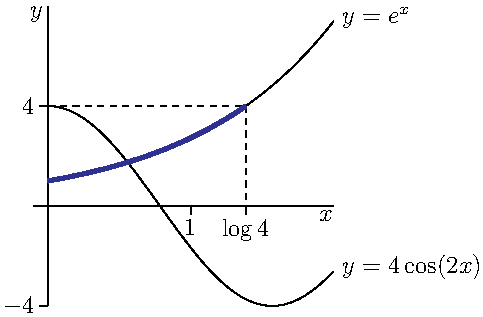
\includegraphics{graphExpCos}
\end{center}

         It sure looks like there is exactly one crossing with $x\ge 0$
         and that one crossing is somewhere between $x=0$ and $x=1$. Indeed
         since $\big[e^x- 4\cos(2x)\big]_{x=0} = -3<0$ and
               $\big[e^x- 4\cos(2x)\big]_{x=1} > e > 0$ and
         $f(x)=e^x- 4\cos(2x)$ is continuous, the intermediate value
         theorem guarantees that there is at least one root with
         $0<x<1$.

         We still have to show that there is no second root --- even if our
         graphs are not accurate.

Recall that the range of the cosine function is $[-1,1]$. If $e^x=4\cos(2x)$, then $e^x \leq 4$, so $x \leq \log(4)\approx 1.39$. So, we only need to search for roots of $f(x)$ on the interval $(0,1.4)$: we are guaranteed there are no roots elsewhere. Over this interval,
$2x \in (0,2.8)$, so $\sin(2x)>0$, and thus $f'(x)=e^x+8\sin(2 x)>0$. Since $f'(x)$ has no roots in $(0,1.4)$, we conclude by Rolle's Theorem that $f(x)$ has at most one root in $(0,1.4)$ (and so at most one positive root total). Since we've already found that a root of $f(x)$ exists in $(0,1)$, we conclude
 $e^x=4\cos(2x)$ has precisely one positive-valued solution.
\end{solution}




\begin{Mquestion}[1997H]
Let $f(x)=3x^5-10x^3+15x+a$, where $a$ is some constant.
\begin{enumerate}[(a)]
\item\label{s2.131997.1}  Prove that, regardless of the value $a$, $f'(x)>0$
for all $x$ in $(-1,1)$.
\item\label{s2.131997.2} Prove that, regardless of the value $a$, $f(x)=3x^5-10x^3+15x+a$
has at most one root in $[-1,1]$.
\end{enumerate}
\end{Mquestion}
\begin{hint} For \eqref{s2.131997.2},  what does Rolle's Theorem tell you has to happen in order for $f(x)$ to have \emph{more than} one root in $[-1,1]$?
\end{hint}
\begin{answer}
\eqref{s2.131997.1} $$
f'(x)=15x^4-30x^2+15=15\big(x^4-2x^2+1\big)=15\big(x^2-1\big)^2\ge 0
$$
The derivative is nonnegative everywhere. The only values of $x$ for which $f'(x)=0$ are $1$ and $-1$, so $f'(x)>0$ for every $x$ in $(-1,1)$.
\smallskip

\eqref{s2.131997.2} If $f(x)$ has two roots $a$ and $b$ in $[-1,1]$, then by Rolle's Theorem, $f'(c)=0$ for some $x$ strictly between $a$ and $b$. But since $a$ and $b$ are in $[-1,1]$, and $c$ is between $a$ and $b$, that means $c$ is in $(-1,1)$; however, we know for every $c$ in $(-1,1)$, $f'(c)>0$, so this can't happen. Therefore, $f(x)$ \emph{does not} have two roots $a$ and $b$ in $[-1,1]$. This means $f(x)$ has at most one root in $[-1,1]$.

\end{answer}
\begin{solution}
\eqref{s2.131997.1} $$
f'(x)=15x^4-30x^2+15=15\big(x^4-2x^2+1\big)=15\big(x^2-1\big)^2\ge 0
$$
The derivative is nonnegative everywhere. The only values of $x$ for which $f'(x)=0$ are $1$ and $-1$, so $f'(x)>0$ for every $x$ in $(-1,1)$.
\smallskip

\eqref{s2.131997.2} If $f(x)$ has two roots $a$ and $b$ in $[-1,1]$, then by Rolle's Theorem, $f'(c)=0$ for some $x$ strictly between $a$ and $b$. But since $a$ and $b$ are in $[-1,1]$, and $c$ is between $a$ and $b$, that means $c$ is in $(-1,1)$; however, we know for every $c$ in $(-1,1)$, $f'(c)>0$, so this can't happen. Therefore, $f(x)$ \emph{does not} have two roots $a$ and $b$ in $[-1,1]$. This means $f(x)$ has at most one root in $[-1,1]$.
\end{solution}


\begin{Mquestion}[2009H]
Find the point promised by the Mean Value Theorem for the function
$e^x$ on the interval $[0, T]$.
\end{Mquestion}
\begin{hint}
Since $f(x)=e^x$ is a continuous and differentiable function, the MVT promises that there exists some number $c$ such that \[f'(c)=\frac{f(T)-f(0)}{T}.\]
Find that $c$, in terms of $T$.
\end{hint}
\begin{answer}
$\log\left(\dfrac{e^T-1}{T}\right)$
\end{answer}
\begin{solution}
Write $f(x)=e^x$. Since $f(x)$ is continuous and differentiable, the Mean Value Theorem asserts that
there exists some $c$ between $0$ and $T$ such that
\begin{align*}
f'(c)&=\frac{f(T)-f(0)}{T-0}
\intertext{The problem asks us to find this value of $c$. Solving:}
 e^c&=\frac{e^T-e^0}{T}\\
e^c&=\frac{e^T-1}{T}\\
 c&=\log\left(\frac{e^T-1}{T}\right)
\end{align*}
\end{solution}


\begin{question}
Use  Corollary~\ref*{cor:DIFFmvtcons} %2.3.11
and Theorem~\ref*{thm:DIFFinvtrigderiv} %2.12.7
in the CLP-1 text to show that $\arcsec x=C-\arccsc x$ for some constant $C$. Find $C$.
\end{question}
\begin{hint}
Let $f(x)=\arcsec x + \arccsc c -C$. %What is the relationship between $\ds\diff{}{x}\arcsec x$ and $\ds\diff{}{x}\{C-\arccsc x\}$?
What is $f'(x)$?
\end{hint}
\begin{answer}
$C=\frac{\pi}{2}$. See the solution for the justification.
\end{answer}
\begin{solution}
The domains of $\arcsec x$ and $C-\arcsec x$ are the same: $|x| \geq 1$.
Define $f(x)=\arcsec x + \arccsc x$, and note that the domain of $f(x)$ is also $|x| \geq 1$.
Using Theorem~\ref*{thm:DIFFinvtrigderiv} in the CLP-1 text,
\begin{equation*}
f'(x)=\diff{}{x}\arcsec x+\diff{}{x} \arccsc x
 = \dfrac{1}{|x|\sqrt{x^2-1}}+\dfrac{-1}{|x|\sqrt{x^2-1}}=0
\end{equation*}
By Corollary~\ref*{cor:DIFFmvtcons} in the CLP-1 text, this means that $f(x)$ 
is constant on any interval in $|x|\ge 1$. So $f(x)$ is a constant, call it $C_+$, on $x\ge 1$, and $f(x)$ is also a constant, call it $C_-$, on $x\le -1$.

In order to find $C_+$, we find $f(1)$, because we know angles for which the secant and cosecant are $x=1$.
\begin{alignat*}{7}
\cos(0)&=1                    &&\implies &\sec(0)&=\tfrac{1}{1}=1 
                              &&\implies &&\arcsec(1)=0
\\
\sin\big(\tfrac{\pi}{2}\big)&=1 
                &&\implies &\csc\big(\tfrac{\pi}{2}\big)&=\tfrac{1}{1}=1 
                &&\implies &&\arccsc(1)=\tfrac{\pi}{2}
\\
        &  && & &  && \implies &&C_+=\arcsec(1)+\arccsc(1)=\tfrac{\pi}{2}
\end{alignat*}
In order to find $C_-$, we find $f(-1)$, because we know angles for which the secant and cosecant are $x=-1$.
\begin{alignat*}{7}
\cos(\pi)&=-1                    &&\implies &\sec(\pi)&=\tfrac{1}{-1}=-1 
                              &&\implies &&\arcsec(-1)=\pi
\\
\sin\big(-\tfrac{\pi}{2}\big)&=-1 
                &&\implies &\csc\big(-\tfrac{\pi}{2}\big)&=\tfrac{1}{-1}=-1 
                &&\implies &&\arccsc(-1)=-\tfrac{\pi}{2}
\\
        &  && & &  && \implies &&C_-=\arcsec(-1)+\arccsc(-1)=\tfrac{\pi}{2}
\end{alignat*}
So $f(x)=\arcsec x + \arccsc x=\frac{\pi}{2}$ for all $|x|\ge 1$
and $\arcsec x = \frac{\pi}{2}- \arccsc x$ for all $|x|\ge 1$.
\end{solution}


%%%%%%%%%%%%%%%%%%
\subsection*{\Application}
%%%%%%%%%%%%%%%%%%


\begin{question}[2009H]
 Suppose $f(0) = 0$ and
$f'(x) = \dfrac{1}{1 + e^{-f(x)}}$ . Prove that $f(100) < 100$.
\medskip

Remark: an equation  relating a function to its own derivative is called a differential equation. We'll see some very basic differential equations in Section~\ref*{sec:ExpGthDecay}.
\end{question}
\begin{hint}
Show that $f$ is differentiable by showing that $f'(x)$ exists for every $x$. Then, the Mean Value Theorem applies. What is the largest $f'(x)$ can be, for any $x$? If $f(100)<100$, what does the MVT tell you must be true of $f'(c)$ for some $c$?
\end{hint}
\begin{answer}
Since $e^{-f(x)}$ is always positive (regardless of the value of $f(x)$),
\[f'(x)=\dfrac{1}{1+e^{-f(x)}}<\dfrac{1}{1+0}=1\] for every $x$.

Since  $f'(x)$ exists for every $x$, we see that $f$ is differentiable, so the Mean Value Theorem applies. If $f(100)$ is greater than or equal to 100, then by the Mean Value Theorem,
 there would have
to be some $c$ between $0$ and $100$ such that
$$
f'(c) = \frac{f(100)-f(0)}{100}\geq\frac{100}{100}= 1
$$

Since $f'(x) \leq 1$ for every $x$, there is \emph{no} value of $c$ as described.
Therefore, it is not possible that  $f(100) \geq 100$. So, $f(100)<100$.
\end{answer}
\begin{solution}
Since $e^{-f(x)}$ is always positive (regardless of the value of $f(x)$),
\[f'(x)=\dfrac{1}{1+e^{-f(x)}}<\dfrac{1}{1+0}=1\] for every $x$.

Since  $f'(x)$ exists for every $x$, we see that $f$ is differentiable, so the Mean Value Theorem applies. If $f(100)$ is greater than or equal to 100, then by the Mean Value Theorem,
 there would have
to be some $c$ between $0$ and $100$ such that
$$
f'(c) = \frac{f(100)-f(0)}{100}\geq\frac{100}{100}= 1
$$

Since $f'(x) < 1$ for every $x$, there is \emph{no} value of $c$ as described.
Therefore, it is not possible that  $f(100) \geq 100$. So, $f(100)<100$.
\end{solution}


\begin{Mquestion}
Let $f(x)=2x+\sin x$. What is the largest interval containing $x=0$ over which  $f(x)$ is one--to--one?  What are the domain and range of $f^{-1}(x)$?
\end{Mquestion}
\begin{hint}
In order for $f^{-1}(x)$ to be defined over an interval, $f(x)$ must be one--to--one over that interval.
\end{hint}
\begin{answer}
Domain of $f^{-1}(x)$: $(-\infty,\infty)$\\
Interval where $f$ is one--to--one, and range of $f^{-1}(x)$: $(-\infty,\infty)$
\end{answer}
\begin{solution}
If $2x+\sin x$ is one--to--one over an interval, it never takes the same value for two distinct numbers in that interval. By Rolle's Theorem, if $f(a)=f(b)$ for distinct $a$ and $b$, then
$f'(c)=0$ for some $c$ between $a$ and $b$. However, $f'(x)=2+\cos x$, which is never zero. In fact, $f'(x)\ge 1$ for all $x$, so $f(x)$ is strictly increasing over its entire domain. Therefore, our function $f$ \emph{never} takes the same value twice, so it is one--to--one over all the real numbers, $(-\infty,\infty)$.

When we define the inverse function $f^{-1}(x)$, the domain of $f$ is the range of $f^{-1}$, and vice-versa. In general, we might have to \emph{restrict} the domain of $f$ (and hence the range of $f^{-1}$) to an interval where $f$ is one--to--one, but in our case, this isn't necessary. So, the range of $f^{-1}$ is $(-\infty,\infty)$ and the domain of $f^{-1}$ is the range of $f$: $(-\infty,\infty)$.
\end{solution}



\begin{question}
Let $f(x)=\dfrac{x}{2}+\sin x$. What is the largest interval containing $x=0$ over which  $f(x)$ is one--to--one?  What are the domain and range of $f^{-1}(x)$, if we restrict $f$ to this interval?
\end{question}
\begin{hint}
In order for $f^{-1}(x)$ to be defined over an interval, $f(x)$ must be one--to--one over that interval.
\end{hint}
\begin{answer}
One--to--one interval, and range of $f^{-1}$: $\left[-\frac{2\pi}{3},\frac{2\pi}{3}\right]$ \\
Domain of $f^{-1}$: $\left[-\left(\frac{\pi}{3}+\frac{\sqrt{3}}{2}\right),\left(\frac{\pi}{3}+\frac{\sqrt{3}}{2}\right)\right]$
\end{answer}
\begin{solution}
If $f(x)=\dfrac{x}{2}+\sin x$ is one--to--one over an interval, it never takes the same value for two distinct numbers in that interval. By Rolle's Theorem, if $f(a)=f(b)$ for distinct $a$ and $b$, then
$f'(c)=0$ for some $c$ between $a$ and $b$. Since $f'(x)=\frac{1}{2}+\cos x$,
$f'(x)=0$ when $x=2n\pi\pm\frac{2\pi}{3}$ for some integer $n$. So, in particular, if  $a$ and $b$ are distinct numbers in the interval $\left[-\frac{2\pi}{3},\frac{2\pi}{3}\right]$, then for every $c$ strictly between $a$ and $b$, $f'(c) \neq 0$, so by Rolle's Theorem $f(a) \neq f(b)$. Therefore $f(x)$ is one--to--one on the interval $\left[-\frac{2\pi}{3},\frac{2\pi}{3}\right]$.

We should also show that the interval $\left[-\frac{2\pi}{3},\frac{2\pi}{3}\right]$ cannot be extended to a larger interval over which $f(x)$ is still one--to--one. %We see that as soon as we let $x$ be a little larger than $\frac{2\pi}{3}$ or a little smaller than $\frac{-2\pi}{3}$, then $f'(x)<0$: so the graph ``reverses direction." % and $f(x)$ repeats values.
Consider the derivative $f'(x) = \frac{1}{2}+\cos x$.
           For all $-\frac{2\pi}{3} < x < \frac{2\pi}{3}$, we have
           $\cos x > -\frac{1}{2}$ (sketch the graph of $\cos x$
           yourself) so that $f'(x)>0$ and $f(x)$ is
           increasing. But at $x=\frac{2\pi}{3}$, $f'(x)=0$, and then
           for $x$ a bit bigger than  $\frac{2\pi}{3}$ we have
           $\cos x < -\frac{1}{2}$ so that $f'(x)<0$ and $f(x)$ is
           decreasing. So the graph ``reverses direction", and $f(x)$
           repeats values. (See the graph of $y=f(x)$ below.) The
           same is true for $x$ a little smaller than $-\frac{2\pi}{3}.$

\begin{center}\begin{tikzpicture}
\YEaxis{3.5}{3.5}
\draw plot[domain=-3.2:3.2](\x,{\x/2+sin(\x r)}) node[right]{$y=f(x)=\dfrac{x}{2}+\sin x$};
\draw (2.1,.2)--(2.1,-.2) node[below]{$\frac{2\pi}{3}$};
\draw (-2.1,.2)--(-2.1,-.2) node[below]{$-\frac{2\pi}{3}$};
\draw (2.1,1.9) node[vertex]{};
\draw (-2.1,-1.9) node[vertex]{};
\end{tikzpicture}\end{center}



When we define the inverse function $f^{-1}(x)$, first we restrict $f$ to $\left[-\frac{2\pi}{3},\frac{2\pi}{3}\right]$. Then the range of $f^{-1}$ is also $\left[-\frac{2\pi}{3},\frac{2\pi}{3}\right]$.  The domain of $f^{-1}$ is the range of $f$ over this interval, so
$\left[-\left(\frac{\pi}{3}+\frac{\sqrt{3}}{2}\right),\left(\frac{\pi}{3}+\frac{\sqrt{3}}{2}\right)\right]$.
\end{solution}


\begin{question}
Suppose $f(x)$ and $g(x)$ are functions that are continuous over the interval $[a,b]$ and differentiable over the interval $(a,b)$. Suppose further that $f(a) < g(a)$ and $g(b)< f(b)$. Show that there exists some $c \in [a,b]$ with $f'(c)>g'(c)$.
\end{question}
\begin{hint}
Let $h(x)=f(x)-g(x)$. What does the Mean Value Theorem tell you about the derivative of $h$?
\end{hint}
\begin{answer}
Define $h(x)=f(x)-g(x)$, and notice $h(a)=f(a)-g(a)<0$ and $h(b)=f(b)-g(b)>0$. Since $h$ is the difference of two functions that are continuous over $[a,b]$ and differentiable over $(a,b)$, also $h$ is continuous over $[a,b]$ and differentiable over $(a,b)$. So, by the Mean Value Theorem, there exists some $c \in (a,b)$ with
\[h'(c)=\frac{h(b)-h(a)}{b-a}\]
Since $(a,b)$ is an interval, $b>a$, so the denominator of the above expression is positive; since $h(b)>0>h(a)$, also the numerator of the above expression is positive. So, $h'(c)>0$ for some $c \in (a,b)$. Since $h'(c)=f'(c)-g'(c)$, we conclude $f'(c)>g'(c)$ for some $c \in (a,b)$.
\end{answer}
\begin{solution}
Define $h(x)=f(x)-g(x)$, and notice $h(a)=f(a)-g(a)<0$ and $h(b)=f(b)-g(b)>0$. Since $h$ is the difference of two functions that are continuous over $[a,b]$ and differentiable over $(a,b)$, also $h$ is continuous over $[a,b]$ and differentiable over $(a,b)$. So, by the Mean Value Theorem, there exists some $c \in (a,b)$ with
\[h'(c)=\frac{h(b)-h(a)}{b-a}\]
Since $(a,b)$ is an interval, $b>a$, so the denominator of the above expression is positive; since $h(b)>0>h(a)$, also the numerator of the above expression is positive. So, $h'(c)>0$ for some $c \in (a,b)$. Since $h'(c)=f'(c)-g'(c)$, we conclude $f'(c)>g'(c)$ for some $c \in (a,b)$.
\end{solution}




\begin{Mquestion}
Suppose $f(x)$ is a function that is differentiable over all real numbers, and $f'(x)$ has precisely two roots. What is the maximum number of distinct roots that $f(x)$ may have?
\end{Mquestion}
\begin{hint}
Rolle's Theorem relates the roots of a function to the roots of its derivative.
\end{hint}
\begin{answer}
$3$
\end{answer}
\begin{solution}
Since $f(x)$ is differentiable over all real numbers, it is also continuous over all real numbers. We claim that $f(x)$ cannot have four or more distinct roots. For every two distinct roots $a<b$, Rolle's Theorem tells us there is a $c \in (a,b)$ such that $f'(c)=0$: that is, $c$ is a root of $f'$. Since $f'$ has only two distinct roots, $f$ can have at most three distinct roots.

\begin{center}
\begin{tikzpicture}
\draw[ultra thick, <->] (0,0)--(6,0);
\color{blue}
\draw (1,.2)--(1,-.2) node[below](a1){$a_1$};
\draw (3,.2)--(3,-.2) node[below](a2){$a_2$};
\draw (5,.2)--(5,-.2) node[below](a3){$a_3$};
\draw (3,-3) node(b){roots of $f(x)$};
\foreach \x in {1,2,3} {\draw[dashed, ->] (b)--(a\x);}
\color{red}
\draw (2,-.2)--(2,.2) node[above](c1){$c_1$};
\draw (4,-.2)--(4,.2) node[above](c2){$c_2$};
\draw (3,3) node(c){roots of $f'(x)$};
\foreach \x in {1,2} {\draw[dashed, ->] (c)--(c\x);}
\end{tikzpicture}\end{center}
\end{solution}



\begin{Mquestion}
How many roots does $f(x)=\sin x + x^2 + 5x +1$ have?
\end{Mquestion}
\begin{hint}
To show that there are exactly $n$ distinct roots, you need to not only show that $n$ exist, but also that there are \emph{not more} than $n$.
\end{hint}
\begin{answer} $2$
\end{answer}
\begin{solution}
We are asked to find the number of solutions to the equation
          $x^2+5x+1 = -\sin x$.  The figure below contains the graphs
          of $y=x^2+5x+1$ and $y=-\sin x$. The solutions to
          $x^2+5x+1 = -\sin x$ are precisely the $x$'s where
          $y=x^2+5x+1$ and $y=-\sin x$ cross.

\begin{center}\begin{tikzpicture}
\YEaaxis{7}{2}{5}{3}
\draw plot[domain=-5.25:.3](\x,{\x*\x+5*\x+1}) node[right]{$y=x^2+5x+1$};
\draw[line width=4pt, blue] plot[domain=-5:-4.56](\x,{\x*\x+5*\x+1});
\draw[line width=4pt, blue] plot[domain=-0.44:0](\x,{\x*\x+5*\x+1});
\draw[ dashed] (-6,1)--(.5,1) node[right]{$y=1$};
\draw[ dashed] (-6,-1)--(.5,-1) node[right]{$y=-1$};
\draw[thick, red] plot[domain=-6.5:.5](\x,{-sin \x r}) node[right]{$y=-\sin x$};
\end{tikzpicture}\end{center}


         From the figure, it sure looks like there are two crossings.
         Since the function $-\sin x$ has range $[-1,1]$,
         if the two functions cross, then also $-1 \leq x^2+5x+1\leq 1 $.
         This portion of the quadratic function is highlighted in blue in the figure.
         The $x$ coordinates of the end points
         of the blue arcs are found by solving $x^2+5x+1 = \pm1$,
         i.e. $x=0$, $-5$, and (using the quadratic equation)
         $x= \frac{-5\pm\sqrt{17}}{2}$.

         We are now in a position
         to exploit the intuition that we have built using the above
         figure to write a concise argument showing that $f(x)$ has exactly
         two roots.
         Remember that, in general, if we want to show that a function has $n$ roots, we need to show that there exist $n$ distinct roots somewhere, and that there do not exist $n+1$ distinct roots. This argument is given below, in blue text.
\color{blue}
\begin{itemize}
\item $f(x)$ is continuous over all real numbers
\item $f(x)=0$ only when $-\sin x=x^2+5x+1$, which only happens when $|x^2+5x+1| \leq 1$. Thus, $f(x)$ only has roots in the intervals
$\left[-5,\frac{-5-\sqrt{17}}{2}\right]$ and $\left[\frac{-5+\sqrt{17}}{2},0\right]$.
\item  $f(-5)=\sin(-5)+1 > 0$, and $f\left(\frac{-5-\sqrt{17}}{2}\right)=\sin\left(\frac{-5-\sqrt{17}}{2}\right)-1 <0$.\\ So, by the IVT, $f(c)=0$ for some
$c \in \left(-5,\frac{-5-\sqrt{17}}{2}\right)$.
\item $f(0)=1>0$, and $f\left(\frac{-5+\sqrt{17}}{2}\right)=\sin\left(\frac{-5+\sqrt{17}}{2}\right)-1<0$.\\ So, by the IVT, $f(c)=0$ for some
$c \in \left(\frac{-5+\sqrt{17}}{2},0\right)$.
\item $f'(x)=\cos x + 2x + 5$. If $f'(x)=0$, then $2x+5=-\cos x$, so $|2x+5| \leq 1$. So, the only interval that can contain roots of $f'(x)$ is $[-3,-2]$.
\item Suppose $f(x)$ has more than two roots. Then it has two roots in the interval
$\left[-5,\frac{-5-\sqrt{17}}{2}\right]$ OR it has two roots in the interval
$\left[\frac{-5+\sqrt{17}}{2},0\right]$. Since $f(x)$ is differentiable for all real numbers,  Rolle's Theorem tells us that $f'(x)$ has a root in $\left(-5,\frac{-5-\sqrt{17}}{2}\right)$ or in $\left(\frac{-5+\sqrt{17}}{2},0\right)$. However, since all roots of $f'(x)$ are in the interval $[-3,-2]$, and this interval shares no points with $\left(-5,\frac{-5-\sqrt{17}}{2}\right)$ or $\left(\frac{-5+\sqrt{17}}{2},0\right)$, this cannot be the case. Therefore $f(x)$ does not have more than two roots.
\begin{center}
\begin{tikzpicture}
\draw[ultra thick, <->] (-12,0)--(2,0);
\color{blue}
\draw (-10,.2)--(-10,-.2) node[below]{$-5$};
%\draw (-9,.2)--(-9,-.2) node[below]{$-4.5$};
\draw (-9,.2)--(-9,-.2) node[below]{$\frac{-5-\sqrt{17}}{2}$};
\draw[line width=4pt] (-10,0)--(-9,0);
%\draw (-1,.2)--(-1,-.2) node[below]{$-0.5$};
\draw (-1,.2)--(-1,-.2) node[below]{$\frac{-5+\sqrt{17}}{2}$};
\draw (0,.2)--(0,-.2) node[below]{$0$};
\draw[line width=4pt] (-1,0)--(0,0);
\draw (-5,-3) node(c){roots of $f(x)$};
\draw [dashed, ->] (c)--(-9.5,-1);
\draw [dashed, ->] (c)--(-.5,-1);
\color{red}
\draw (-6,-.2)--(-6,.2) node[above]{$-3$};
\draw (-4,-.2)--(-4,.2) node[above]{$-2$};
\draw[line width=4pt] (-6,0)--(-4,0);
\draw (-5,3) node(d){roots of $f'(x)$};
\draw [dashed, ->] (d)--(-5,1);
\end{tikzpicture}
\end{center}
\item Since $f(x)$ has at least two roots, and not more than two roots, $f(x)$ has exactly two roots.
\end{itemize}

\color{black}


%It's not easy to find a root of $f(x)$ by inspection, but we notice the following:
%\begin{itemize}
%\item $f(x)$ is continuous for all real numbers
%\item $f(0)=1>0$
%\item $f(-\pi)=\pi^2-5\pi+1<0$
%\end{itemize}
%So, by the Intermediate Value Theorem, $f(x)$ has a root in the interval $(-\pi,0)$.
%Now, let's think about the roots of $f'(x)=\cos x + 2x + 5$. This function has at least one root (again, we can use IVT: $f(0)=6>0$, and $f(-\pi)=-2\pi+4<0$) so it's possible that $f(x)$ has two or more roots.
%
%At this point, we don't know much: $f(x)$ has at least one root. If $f'(x)$ were a function with no roots, we'd be done, but such is not the case. So, we decide to be more careful. Rolle's Theorem tells us that, if $f(a)=f(b)=0$ and $a \neq b$, then $f'(c)=0$ for some $c$ strictly between $a$ and $b$. So, let's look at where $f$ and $f'$ could have roots.
%
%If $f(x)=0$, then $x^2+5x+1=-\sin x$, so $|x^2+5x+1| \leq 1$. Let's figure out which values of $x$ this corresponds to. The function $x^2+5x+1$ is an upwards-pointing parabola. $x^2+5x+1=1$ when $x=0$ and $x=-5$, and
% $x^2+5x+1=-1$ when $x=\dfrac{-5\pm\sqrt{17}}{2}$, or  $x \approx -4.56$ and $x \approx -0.44$. Therefore, all roots of $f(x)$ are in the intervals $\left[-5,\dfrac{-5-\sqrt{17}}{2}\right] $ and $\left[\dfrac{-5+\sqrt{17}}{2},0\right]$.
%
%Now, let's consider where $f'(x)$ can be zero. If $0=f'(x)=\cos x + 2x +5$, then $2x+5=\cos x$, so $|2x+5| \leq 1$. Therefore $f'(x)$ only has roots in the interval $[-2,-3,]$.
%By Rolle's Theorem, there can be at most one root of $f(x)$ in the interval $\left[\frac{-5+\sqrt{17}}{2},0\right]$ (otherwise there would be a root of $f'(x)$ in$\left(\frac{-5+\sqrt{17}}{2},0\right)$, which isn't true) and  there can be at most one root of $f(x)$ in the interval $\left[-5,\frac{-5-\sqrt{17}}{2}\right]$ (otherwise there would be a root of $f'(x)$ in $\left(-5,\frac{-5-\sqrt{17}}{2}\right)$ , which isn't true). We already know that $f(0)=0$, so $0$ is the only root of $f(x)$ outside of the interval $\left[-5,\frac{-5-\sqrt{17}}{2}\right]$ . Let's investigate this interval further. At its endpoints: $f(-5)=\sin(-5)+1 > 0$, and $f\left(\frac{-5-\sqrt{17}}{2}\right)=\sin\left(\frac{-5-\sqrt{17}}{2}\right)-1 <0$. So, since $f(x)$ is continuous over all real numbers, by the IVT, $f(x)$ has a root in this interval.
\end{solution}

\section{Higher Order Derivatives}
%
% Copyright 2018 Joel Feldman, Andrew Rechnitzer and Elyse Yeager.
% This work is licensed under a Creative Commons Attribution-NonCommercial-ShareAlike 4.0 International License.
% https://creativecommons.org/licenses/by-nc-sa/4.0/
%

\questionheader{ex:s2.14}
%%%%%%%%%%%%%%%%%%
\subsection*{\Conceptual}
%%%%%%%%%%%%%%%%%%




\begin{question}What is the 180th derivative of the function $f(x)=e^x$?
\end{question}
\begin{hint} If you know the first derivative, this should be easy.
\end{hint}
\begin{answer} $e^x$
\end{answer}
\begin{solution} The derivative of $e^x$ is $e^x$: taking derivatives leaves the function unchanged, even if we do it 180 times. So $f^{(180)}=e^x$.
\end{solution}




\begin{Mquestion}
Suppose $f(x)$ is a differentiable function, with $f'(x)>0$ and $f''(x)>0$ for every $x \in (a,b)$. Which of the following must be true?
\begin{enumerate}[(i)]
\item\label{s2.14''i} $f(x)$ is positive over $(a,b)$
\item\label{s2.14''ii} $f(x)$ is increasing over $(a,b)$
\item\label{s2.14''iii} $f(x)$ is increasing at a constant rate over $(a,b)$
\item\label{s2.14''iv} $f(x)$ is increasing faster and faster over $(a,b)$
\item\label{s2.14''v} $f'''(x)>0$ for some $x \in (a,b)$
\end{enumerate}
\end{Mquestion}
\begin{hint} Exactly two of the statements must be true.
\end{hint}
\begin{answer}
\eqref{s2.14''ii}, \eqref{s2.14''iv}
\end{answer}
\begin{solution}
Since $f'(x)>0$ over $(a,b)$, we know from Corollary~\ref*{cor:DIFFmvtcons}
that $f(x)$ is increasing over $(a,b)$, so \eqref{s2.14''ii} holds. Since $f''(x)>0$, and $f''(x)$ is the derivative of $f'(x)$, by the same reasoning we see that $f'(x)$ is increasing. Since $f'(x)$ is the rate at which $f(x)$ is increasing, that means that the rate at which $f'(x)$ is increasing is itself increasing: this is, \eqref{s2.14''iv} holds (and \emph{not} \eqref{s2.14''iii}).

There is no reason to think \eqref{s2.14''i} or \eqref{s2.14''v} holds, but to be thorough we will give an example showing that they do not need to be true. If $f(x)=x^2-10$ and $(a,b)=(0,1)$, then $f'(x)=2x>0$ over $(0,1)$, and $f''(x)=2>0$ everywhere, but $f(x)<0$ for all $x \in (0,1)$, so \eqref{s2.14''i} does not hold. Also, $f'''(x)=0$ everywhere, so \eqref{s2.14''v} does not hold either.
\end{solution}







\begin{question}
Let $f(x)=ax^{15}$ for some constant $a$. Which value of $a$ results in $f^{(15)}(x)=3$?
\end{question}
\begin{hint}
Use factorials, as in Example~\ref*{eg:higherOrdDerivA}.
\end{hint}
\begin{answer}
$\dfrac{3}{15!}$
\end{answer}
\begin{solution}
Every time we differentiate $f(x)$, the constant out front gets multiplied by an ever-decreasing constant, while the power decreases by one. As in Example~\ref*{eg:higherOrdDerivA}, $\ds\ddiff{{15}}{}{x}ax^{15}=a\cdot 15!$. So, if $a\cdot 15!=3$, then $a=\dfrac{3}{15!}$.
\end{solution}




\begin{Mquestion}
Find the mistake(s) in the following work, and provide a corrected answer.
\begin{quote}
Suppose $-14x^2+2xy+y^2=1$. We find $\ds\ddiff{2}{y}{x}$ at the point $\left(1,3\right)$. Differentiating implicitly:
\begin{align*}
-28x+2y+2xy'+2yy'&=0
\intertext{Plugging in $x=1$, $y=3$:}
-28+6+2y'+6y'&=0\\
y'&=\frac{11}{4}
\intertext{Differentiating:}
y''&=0
\end{align*}
\end{quote}
\end{Mquestion}
\begin{hint}
The problem isn't with any of the algebra.
\end{hint}
\begin{answer}
The derivative $\ds\diff{y}{x}$ is $\dfrac{11}{4}$ only at the point $(1,3)$: it is not \emph{constantly} $\dfrac{11}{4}$, so it is wrong to differentiate the constant $\dfrac{11}{4}$ to find $\ds\ddiff{2}{y}{x}$. Below is a correct solution.
\begin{align*}
-28x+2y+2xy'+2yy'&=0
\intertext{Plugging in $x=1$, $y=3$:}
-28+6+2y'+6y'&=0\\
y'&=\frac{11}{4} \quad\mbox{\textcolor{red}{ at the point $(1,3)$}}
\intertext{Differentiating \textcolor{red}{the equation $-28x+2y+2xy'+2yy'=0$}:}
-28+2y'+2y'+2xy''+2y'y'+2yy''&=0\\
4y'+2(y')^2+2xy''+2yy''&=28
\intertext{At the point $(1,3)$, $y'=\dfrac{11}{4}$. Plugging in:}
4\left(\frac{11}{4}\right)+2\left(\frac{11}{4}\right)^2+2(1)y''+2(3)y''&=28\\
y''&=\frac{15}{64}
\end{align*}
\end{answer}
\begin{solution}
The derivative $\ds\diff{y}{x}$ is $\dfrac{11}{4}$ only at the point $(1,3)$: it is not \emph{constantly} $\dfrac{11}{4}$, so it is wrong to differentiate the constant $\dfrac{11}{4}$ to find $\ds\ddiff{2}{y}{x}$. Below is a correct solution.
\begin{align*}
-28x+2y+2xy'+2yy'&=0
\intertext{Plugging in $x=1$, $y=3$:}
-28+6+2y'+6y'&=0\\
y'&=\frac{11}{4} \quad\mbox{\textcolor{red}{ at the point $(1,3)$}}
\intertext{Differentiating \textcolor{red}{the equation $-28x+2y+2xy'+2yy'=0$}:}
-28+2y'+2y'+2xy''+2y'y'+2yy''&=0\\
4y'+2(y')^2+2xy''+2yy''&=28
\intertext{At the point $(1,3)$, $y'=\dfrac{11}{4}$. Plugging in:}
4\left(\frac{11}{4}\right)+2\left(\frac{11}{4}\right)^2+2(1)y''+2(3)y''&=28\\
y''&=\frac{15}{64}
\end{align*}
\end{solution}



%%%%%%%%%%%%%%%%%%
\subsection*{\Procedural}
%%%%%%%%%%%%%%%%%%



\begin{question}
Let $f(x)=(\log x-1)x$. Evaluate $f''(x)$.
\end{question}
\begin{hint}
Recall $\ds\diff{}{x}\log x =\ds\frac{1}{x}$.
\end{hint}
\begin{answer}
$f''(x)=\dfrac{1}{x}$
\end{answer}
\begin{solution}
\begin{align*}
f(x)&=x\log x -x\\
f'(x)&=\log x +x\cdot\frac{1}{x}-1\\
&=\log x\\
f''(x)&=\frac{1}{x}
\end{align*}
\end{solution}






\begin{Mquestion}
Evaluate $\ds\ddiff{2}{}{x}\{\arctan x\}$.
\end{Mquestion}
\begin{hint}
Recall $\ds\diff{}{x}\{\arctan x\}=\dfrac{1}{1+x^2}=(1+x^2)^{-1}$.
\end{hint}
\begin{answer}
$\ds\ddiff{2}{}{x}\{\arctan x\}=\frac{-2x}{(1+x^2)^2}$
\end{answer}
\begin{solution}
\begin{align*}
\diff{}{x}\{\arctan x\}&=\frac{1}{1+x^2}\\
\diff{}{x}\left\{\frac{1}{1+x^2}\right\}&=\diff{}{x}\left\{(1+x^2)^{-1}\right\}\\
&=(-1)(1+x^2)^{-2}(2x)\\&=\frac{-2x}{(1+x^2)^2}
\end{align*}
\end{solution}


\begin{question}
The unit circle consists of all point $x^2+y^2=1$. Give an expression for $\ds\ddiff{2}{y}{x}$ in terms of $y$.
\end{question}
\begin{hint}
Use implicit differentiation.
\end{hint}
\begin{answer}
$\ds\ddiff{2}{y}{x}=\dfrac{-1}{y^3}$
\end{answer}
\begin{solution}
We use implicit differentiation, twice.
\begin{align*}
2x+2yy'&=0\\
2+(2y)y''+(2y')y'&=0\\
y''&=-\frac{(y')^2+1}{y}
\intertext{So, we need an expression for $y'$. We use the equation $2x+2yy'=0$ to conclude $y'=-\dfrac{x}{y}$:}
y''&=-\frac{\left(-\frac{x}{y}\right)^2+1}{y}\\
&=-\frac{\frac{x^2}{y^2}+1}{y}\\
&=-\frac{x^2+y^2}{y^3}\\
&=-\frac{1}{y^3}
\end{align*}
\end{solution}


\begin{Mquestion}
Suppose the position of a particle at time $t$ is given by $s(t) = \dfrac{e^t}{t^2+1}$. Find the acceleration of the particle at time $t=1$.
\end{Mquestion}
\begin{hint}
The acceleration is given by $s''(t)$.
\end{hint}
\begin{answer}
$0$
\end{answer}
\begin{solution}
The question asks for $s''(1)$. We start our differentiation using the quotient rule:
\begin{align*}
s'(t)&=\frac{e^t(t^2+1)-e^t(2t)}{(t^2+1)^2}\\
&=\frac{e^t(t^2-2t+1)}{(t^2+1)^2}
\intertext{Using the quotient rule again,}
s''(t)&=\frac{(t^2+1)^2\textcolor{blue}{\diff{}{t}\{e^t(t^2-2t+1)\}}-e^t(t^2-2t+1) \textcolor{red}{\diff{}{t}\{(t^2+1)^2\}}}{(t^2+1)^4}\\
&=\frac{(t^2+1)^2\cdot\left[\textcolor{blue}{e^t(2t-2)+e^t(t^2-2t+1)}\right]-
e^t(t^2-2t+1) \cdot \textcolor{red}{2(t^2+1)(2t)}}{(t^2+1)^4}\\
&=\frac{e^t(t^2+1)^2(t^2-1)-4te^t(t-1)^2(t^2+1)}{(t^2+1)^4}\\
s''(1)&=0
\end{align*}
\end{solution}



\begin{question}
Evaluate $\ds\ddiff{3}{}{x}\{\log(5x^2-12)\}$.
\end{question}
\begin{hint}
Remember to use the chain rule.
\end{hint}
\begin{answer}
$\ds\ddiff{3}{}{x}\{\log(5x^2-12)\}=\frac{100x(5x^2+36)}{(5x^2-12)^3}$
\end{answer}
\begin{solution}
We differentiate using the chain rule.
\begin{align*}
\diff{}{x}\{\log(5x^2-12)\}&=\frac{10x}{5x^2-12}
\intertext{Using the quotient rule:}
\ddiff{2}{}{x}\{\log(5x^2-12)\}&=\diff{}{x}\left\{\frac{10x}{5x^2-12}\right\}\\
&=\frac{(5x^2-12)(10)-10x(10x)}{(5x^2-12)^2}\\
&=\frac{-10(5x^2+12)}{(5x^2-12)^2}
\intertext{Using the quotient rule one last time:}
\ddiff{3}{}{x}\{\log(5x^2-12)\}&=\diff{}{x}\left\{
\frac{-10(5x^2+12)}{(5x^2-12)^2}
\right\}\\
&=\frac{(5x^2-12)^2(-10)(10x)+10(5x^2+12)(2)(5x^2-12)(10x)}{(5x^2-12)^4}\\
&=\frac{(5x^2-12)(-100x)+(200x)(5x^2+12)}{(5x^2-12)^3}\\
&=\frac{100x(-5x^2+12+10x^2+24)}{(5x^2-12)^3}\\
&=\frac{100x(5x^2+36)}{(5x^2-12)^3}
\end{align*}
\end{solution}






\begin{question}
The height of a particle at time $t$ seconds is given by $h(t)=-\cos t$. Is the particle speeding up or slowing down at $t=1$?
\end{question}
\begin{hint}
$h'(t)$ gives the velocity of the particle, and $h''(t)$ gives its acceleration--the rate the velocity is changing.
\end{hint}
\begin{answer}
speeding up
\end{answer}
\begin{solution}
The velocity of the particle is given by $h'(t)=\sin t$. Note $0<1<\pi$, so
$h'(1)>0$--the particle is rising (moving in the positive direction, in this case ``up").
The acceleration of the particle is $h''(t)=\cos t$. Since $0<1<\frac{\pi}{2}$, $h''(t)>0$, so $h'(t)$ is increasing: the particle is moving up, and it's doing so at an increasing rate. So, the particle is speeding up.
\end{solution}

\begin{Mquestion}
The height of a particle at time $t$ seconds is given by $h(t)=t^3-t^2-5t+10$. Is the particle's motion getting faster or slower at $t=1$?
\end{Mquestion}
\begin{hint}
$h'(t)$ gives the velocity of the particle, and $h''(t)$ gives its acceleration--the rate the velocity is changing. Be wary of signs--as in legends, they may be misleading.
\end{hint}
\begin{answer}
slower
\end{answer}
\begin{solution}
For this problem, remember that velocity has a sign indicating direction, while speed does not.

The velocity of the particle is given by $h'(t)=3t^2-2t-5$. At $t=1$, the velocity of the particle is $-4$, so the particle is moving downwards with a speed of 4 units per second. The acceleration of the particle is $h''(t)=6t-2$, so when $t=1$, the acceleration is (positive) $4$ units per second per second. That means the velocity (currently $-4$ units per second) is becoming a bigger number--since the velocity is negative, a bigger number is closer to zero, so the speed of the particle is getting smaller. (For instance, a velocity of $-3$ represents a slower motion than a velocity of $-4$.) So, the particle is  slowing down at $t=1$.
\end{solution}



\begin{question}
Suppose a curve is defined implicitly by
\[x^2+x+y=\sin(xy)\]
What is $\ds\ddiff{2}{y}{x}$ at the point $(0,0)$?
\end{question}
\begin{hint}
You don't need to solve for $y''$ in general--only when $x=y=0$. To do this, you \emph{also} need to find $y'$ at the point $(0,0)$.
\end{hint}
\begin{answer}
$-4$
\end{answer}
\begin{solution}
\begin{align*}
x^2+x+y&=\sin(xy)
\intertext{We differentiate implicitly. For ease of notation, we write $y'$ for $\ds\diff{y}{x}$.}
2x+1+y'&=\cos(xy)(y+xy')
\intertext{We're interested in $y''$, so we implicitly differentiate again.}
2+y''&=-\sin(xy)(y+xy')^2+\cos(xy)(2y'+xy'')
\intertext{We want to know what $y''$ is when $x=y=0$. Plugging these in yields the following:}
2+y''&=2y'
\intertext{So, we need to know what $y'$ is when $x=y=0$. We can get this from the equation $2x+1+y'=\cos(xy)(y+xy')$, which becomes
$1+y'=0$ when $x=y=0$. So, at the origin, $y'=-1$, and}
2+y''&=2(-1)\\
y''&=-4
\end{align*}
Remark: a common mistake is to stop at the equation
$2x+1+y'=\cos(xy)(y+xy')$, plug in $x=y=0$, find $y'=-1$, and decide $y''=\ds\diff{}{x}\{-1\}=0$. This is due to a slight sloppiness in the usual notation. When we wrote $y'=1$, what we meant is that \emph{at the point} $(0,0)$, $\ds\diff{y}{x}=-1$. More properly written: $\left.\ds\diff{y}{x}\right|_{x=0,~y=0}=-1$. This is not the same as saying $y'=1$ everywhere (in which case, indeed, $y''$ would be 0 everywhere).
\end{solution}





\begin{Mquestion}
Which statements below are true, and which false?
\begin{enumerate}[(a)]
\item $\ds\ddiff{4}{}{x} \sin x = \sin x$
\item $\ds\ddiff{4}{}{x} \cos x = \cos x$
\item $\ds\ddiff{4}{}{x} \tan x = \tan x$
\end{enumerate}
\end{Mquestion}
\begin{hint}
To show that two functions are unequal, you can show that one input results in different outputs.
\end{hint}
\begin{answer}
(a) true \qquad (b) true \qquad (c) false
\end{answer}
\begin{solution}
For (a) and (b), notice the following:
\begin{align*}
\diff{}{x} \sin x &= \cos x\\
\diff{}{x} \cos x &= -\sin x\\
\diff{}{x} \{-\sin x\} &= -\cos x\\
\diff{}{x} \{-\cos x\} &= \sin x\\
\diff{}{x} \sin x &= \cos x
\intertext{The fourth derivative is $\sin x$ is $\sin x$, and the fourth derivative of $\cos x$ is $\cos x$, so (a) and (b) are true.}
\diff{}{x}\tan x &=\sec^2 x\\
\diff{}{x}\sec^2 x &=2\sec x (\sec x \tan x)=2\sec^2x\tan x\\
\diff{}{x}\{2\sec^2x\tan x\}&=(4\sec x \cdot \sec x \tan x)\tan x+2\sec^2x\sec^2x\\
&=4\sec^2x\tan^2x+2\sec^4x\\
\diff{}{x}\{4\sec^2x\tan^2x+2\sec^4x\}&=(8\sec x \cdot \sec x \tan x)\tan^2x+4\sec^2x(2\tan x \cdot\sec^2x)\\&\quad+8\sec^3x\cdot\sec x \tan x\\
&=8\sec^2x\tan^3x+16\sec^4x\tan x
\end{align*}
So, $\ds\ddiff{4}{}{x} \tan x =8\sec^2x\tan^3x+16\sec^4x\tan x$. It certainly seems like this is not the same as $\tan x$, but remember that sometimes trig identities can fool you: $\tan^2x+1=\sec^2x$, and so on. So, to be absolutely sure that these are not equal, we need to find a value of $x$ so that the output of one is not the same as the output of the other. When $x=\frac{\pi}{4}$:
\[8\sec^2x\tan^3x+16\sec^4x\tan x = 8\left({\sqrt{2}}\right)^2(1)^3+16\left({\sqrt{2}}\right)^4(1)=80\neq 1=\tan x.\]
So, (c) is false.
\end{solution}




%%%%%%%%%%%%%%%%%%
\subsection*{\Application}
%%%%%%%%%%%%%%%%%%

\begin{Mquestion}
A function $f(x)$ satisfies $f'(x)<0$ and $f''(x)>0$ over $(a,b)$. Which of the following curves below might represent $y=f(x)$?
\begin{center}
\begin{tikzpicture}
\YEaaxis{1}{3}{1}{2}
\YExcoord{.5}{a}
\YExcoord{2.5}{b}
\draw[thick] plot[domain=.5:2.5](\x,{\x*\x*\x*\x/35+.5});
\draw (1.5,-1.5) node{(i)};
\end{tikzpicture}\hfill
\begin{tikzpicture}
\YEaaxis{1}{3}{1}{2}
\YExcoord{.5}{a}
\YExcoord{2.5}{b}
\draw[thick] plot[domain=.5:2.5](3-\x,{\x*\x*\x*\x/35+.5});
\draw (1.5,-1.5) node{(ii)};
\end{tikzpicture}\hfill
\begin{tikzpicture}
\YEaaxis{1}{3}{1}{2}
\YExcoord{.5}{a}
\YExcoord{2.5}{b}
\draw[thick] plot[domain=.5:2.5](\x,{1.5-\x*\x*\x*\x/35});
\draw (1.5,-1.5) node{(iii)};
\end{tikzpicture}

\hfill
\begin{tikzpicture}
\YEaaxis{1}{3}{1}{2}
\YExcoord{.5}{a}
\YExcoord{2.5}{b}
\draw[thick] plot[domain=.5:2.5](3-\x,{1.5-\x*\x*\x*\x/35+.5});
\draw (1.5,-1.5) node{(iv)};
\end{tikzpicture}\hfill
\begin{tikzpicture}
\YEaaxis{1}{3}{1}{2}
\YExcoord{.5}{a}
\YExcoord{2.5}{b}
\draw[thick] plot[domain=.5:2.5](\x,{2.25-\x*.75});
\draw (1.5,-1.5) node{(v)};
\end{tikzpicture}
\hfill~
\end{center}
\end{Mquestion}
\begin{hint} Only one of the curves could possibly represent $y=f(x)$.
\end{hint}
\begin{answer} (ii)
\end{answer}
\begin{solution}
Since $f'(x)<0$, we need a decreasing function. This only applies to (ii), (iii), and  (v). Since $f''(x)>0$, that means $f'(x)$ is increasing, so the \emph{slope} of the function must be increasing. In (v), the slope is constant, so $f''(x)=0$--therefore, it's not (v).
In (iii), the slope is decreasing, because near $a$ the curve is quite flat ($f'(x)$ near zero) but near $b$ the curve is very steeply decreasing ($f'(x)$ is a large \emph{negative} number), so (iii) has a negative second derivative. By contrast, in (ii), the line starts out as steeply decreasing ($f'(x)$ is a strongly negative number) and becomes flatter and flatter ($f'(x)$ nears 0), so $f'(x)$ is increasing--in other words, $f''(x)>0$. So, (ii) is the only curve that has $f'(x)<0$ and $f''(x)>0$.
\end{solution}



\begin{question}
Let $f(x)=2^{x}$. What is $f^{(n)}(x)$, if $n$ is a whole number?
\end{question}
\begin{hint}
Remember $\ds\diff{}{x}\{2^x\}=2^x\log2$.
\end{hint}
\begin{answer}
$f^{(n)}=2^x(\log 2)^n$
\end{answer}
\begin{solution}
We differentiate a few time to find the pattern.
\begin{align*}
\diff{}{x}\{2^x\}&=2^x\log 2\\
\ddiff{2}{}{x}\{2^x\}&=2^x\log2 \cdot \log 2 = 2^x(\log2)^2\\
\ddiff{3}{}{x}\{2^x\}&=2^x(\log2)^2 \cdot \log 2 = 2^x(\log2)^3
\intertext{Every time we differentiate, we multiply the original function by another factor of $\log 2$. So, the $n$th derivative is given by:}
\ddiff{n}{}{x}\{2^x\}&=2^x(\log2)^n
\end{align*}
\end{solution}



\begin{Mquestion}
Let $f(x)=ax^3+bx^2+cx+d$, where $a$, $b$, $c$, and $d$ are nonzero constants.
What is the smallest integer $n$ so that $\ds\ddiff{n}{f}{x}=0$ for all $x$?
\end{Mquestion}
\begin{hint}
Differentiate a few times until you get zero, remembering that $a$, $b$, $c$, and $d$ are all constants.
\end{hint}
\begin{answer}
 $n=4$
\end{answer}
\begin{solution}
We differentiate using the power rule.
\begin{align*}
\diff{f}{x}&=3ax^2+2bx+c\\
\ddiff{2}{f}{x}&=6ax+2b\\
\ddiff{3}{f}{x}&=6a\\
\ddiff{4}{f}{x}&=0
\end{align*}
In the above work, remember that $a$, $b$, $c$, and $d$ are all constants. Since they are nonzero constants, $\ds\ddiff{3}{f}{x} =6a\neq 0$. So, the fourth derivative is the first derivative to be identically zero: $n=4$.
\end{solution}


\begin{question}[1999H]
\[f(x)=e^{x+x^2}\qquad \qquad \qquad h(x)=1+x+\frac{3}{2}x^2\]
\begin{enumerate}[(a)]
\item\label{s2.14ineq1} Find the first and second derivatives of both functions
\item\label{s2.14ineq2} Evaluate both functions and their first and second derivatives at 0.
\item\label{s2.14ineq3} Show that for all $x>0$, $f(x)>h(x)$.
\end{enumerate}
Remark: for some applications, we only need to know that a function is ``big enough." Since $f(x)$ is a difficult function to evaluate, it may be useful to know that it is bigger than $h(x)$ when $x$ is positive.
\end{question}
\begin{hint} Use a similar method to Question~\ref{s2.9ineq}, Section~\ref*{sec chain rule}.
\end{hint}
\begin{answer}
\eqref{s2.14ineq1} $f'(x)=(1+2x)e^{x+x^2}$ \quad $f''(x)=(4x^2+4x+3)e^{x+x^2}$\quad
 $h'(x)=1+3x$ \quad $h''(x)=3$\\
\eqref{s2.14ineq2} $f(0)=h(0)=1$; \quad $f'(0)=h'(0)=1$; \quad $f''(0)=h''(0)=3$\\
\eqref{s2.14ineq3} $f$ and $h$ ``start at the same place," since $f(0)=h(0)$. Also $f'(0)=h'(0)$, and $f''(x)=(4x^2+4x+3)e^{x+x^2} > 3e^{x+x^2}>3=h''(x)$ when $x>0$. Since $f'(0)=h'(0)$, and since $f'$ grows faster than $h'$ for positive $x$, we conclude $f'(x)>h'(x)$ for all positive $x$. Now we can conclude that (since $f(0)=h(0)$ and $f$ grows faster than $h$ when $x>0$) also $f(x)>h(x)$ for all positive $x$.
\end{answer}
\begin{solution}
\eqref{s2.14ineq1}
Using the chain rule for $f(x)$:
\begin{align*}
f'(x)&=(1+2x)e^{x+x^2}\\
f''(x)&=(1+2x)(1+2x)e^{x+x^2}+(2)e^{x+x^2}=(4x^2+4x+3)e^{x+x^2}\\
h'(x)&=1+3x\\
h''(x)&=3
\end{align*}

\eqref{s2.14ineq2} $f(0)=h(0)=1$; \quad $f'(0)=h'(0)=1$; \quad $f''(0)=h''(0)=3$\\
\eqref{s2.14ineq3} $f$ and $h$ ``start at the same place," since $f(0)=h(0)$. If it were clear that $f'(x)$ were greater than $h'(x)$ for $x>0$, then we  would know that $f$ grows faster than $h$, so we could conclude that $f(x)>h(x)$, as desired. Unfortunately, it is not obvious whether $(1+2x)e^{x+x^2}$ is always greater than $1+3x$ for positive $x$. So, we look to the second derivative. $f'(0)=h'(0)$, and $f''(x)=(4x^2+4x+3)e^{x+x^2} > 3e^{x+x^2}>3=h''(x)$ when $x>0$. Since $f'(0)=h'(0)$, and since $f'$ grows faster than $h'$ for positive $x$, we conclude $f'(x)>h'(x)$ for all positive $x$. Now we can conclude that (since $f(0)=h(0)$ and $f$ grows faster than $h$ when $x>0$) also $f(x)>h(x)$ for all positive $x$.
\end{solution}


\begin{question}[1997D]
 The equation $x^3y+y^3=10x$ defines $y$ implicitly as a function
of $x$ near the point $(1,2)$.
\begin{enumerate}[(a)]
\item\label{s2.11p2.1} Compute $y'$ at this point.
\item\label{s2.11p2.2} It can be shown that $y''$ is negative when $x=1$. Use this
fact and your answer to \eqref{s2.11p2.1} to make a sketch showing the relationship of
the curve to its tangent line at $(1,2)$.
\end{enumerate}
\end{question}
\begin{hint} For \eqref{s2.11p2.2}, you know a point where the curve and tangent line intersect, and you know what the tangent line looks like. What do the derivatives tell you about the shape of the curve?
\end{hint}
\begin{answer}
\begin{enumerate}[(a)]
\item $y'(1)=\dfrac{4}{13}$
\item ~
\begin{center}
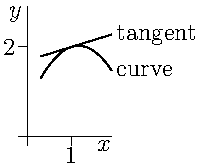
\includegraphics{graphE3}
\end{center}
\end{enumerate}
\end{answer}
\begin{solution}
\begin{enumerate}[(a)]
\item
We differentiate implicitly.
\begin{align*}
x^3y(x)+y(x)^3&=10 x\\
3x^2y(x)+x^3y'(x)+3y(x)^2y'(x)&=10
\intertext{Subbing in $x=1$ and $y(1)=2$ gives}
(3)(1)( 2)+(1)y'(1)+(3)(4) y'(1)&=10\\
13y'(1)&=4\\
y'(1)&=\frac{4}{13}
\end{align*}

\item
 From part \eqref{s2.11p2.1}, the slope of the curve at $x=1,\ y=2$ is $\dfrac{4}{13}$,
so the curve is increasing, but fairly slowly. The angle of the tangent
line is $\tan^{-1}\left(\frac{4}{13}\right)\approx 17^\circ$. We are also told that $y''(1)<0$.
So the slope of the curve is decreasing as $x$ passes through 1. That is, the line is more steeply increasing to the left of $x=1$, and its slope is decreasing (getting less sleep, then possibly the slope even becomes negative) as we move past $x=1$.
%\figput{graphE3}
\begin{center}
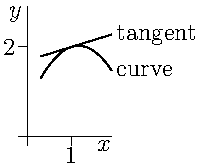
\includegraphics{graphE3}
\end{center}
\end{enumerate}
\end{solution}


\begin{question}\label{s2.14expprod}
Let $g(x)=f(x)e^x$.
In Question~\ref{s2.7expprod}, Section~\ref*{sec exp func}, we learned that $g'(x)=[f(x)+f'(x)]e^x$.
\begin{enumerate}[(a)]
\item\label{s2.14expprod1} What is $g''(x)$?
\item\label{s2.14expprod2} What is $g'''(x)$?
\item\label{s2.14expprod3} Based on your answers above, guess a formula for $g^{(4)}(x)$. Check it by differentiating.
\end{enumerate}
\end{question}
\begin{hint}
Review Pascal's Triangle.
\end{hint}
\begin{answer}
\eqref{s2.14expprod1} $g''(x)=[f(x)+2f'(x)+f''(x)]e^x$\\
\eqref{s2.14expprod2}  $g'''(x)=[f(x)+3f'(x)+3f''(x)+f'''(x)]e^x$\\
\eqref{s2.14expprod3} $g^{(4)}(x)=[f(x)+4f'(x)+6f''(x)+4f'''(x)+f^{(4)}(x)]e^x$
\end{answer}
\begin{solution}
\eqref{s2.14expprod1} Using the product rule, \[g''(x)=[f'(x)+f''(x)]e^x+[f(x)+f'(x)]e^x=[f(x)+2f'(x)+f''(x)]e^x\]

\eqref{s2.14expprod2}  Using the product rule and our answer from~\eqref{s2.14expprod1},
\begin{align*}
g'''(x)&=[f'(x)+2f''(x)+f'''(x)]e^x+[f(x)+2f'(x)+f''(x)]e^x\\
&=[f(x)+3f'(x)+3f''(x)+f'''(x)]e^x
\end{align*}

\eqref{s2.14expprod3} We notice that the coefficients of the derivatives of $f$ correspond to the entries in the rows of Pascal's Triangle.
\begin{center}\begin{tikzpicture}
\draw (0,3) node{1};
\draw (-.5,2.5) node{1}; \draw (.5,2.5) node{1};
\draw (-1,2) node{1}; \draw (1,2) node{1}; \draw (0,2) node{2};
\draw (-1.5,1.5) node{1}; \draw (1.5,1.5) node{1}; \draw (-.5,1.5) node{3}; \draw (.5,1.5) node{3};
\draw (-2,1) node{1}; \draw (2,1) node{1}; \draw (-1,1) node{4}; \draw (1,1) node{4}; \draw (0,1) node{6};
\draw (0,0) node{Pascal's Triangle};
\end{tikzpicture}\end{center}
\begin{itemize}
\item In the first derivative of $g$, the coefficients of $f$ and $f'$ correspond to the entries in the second row of Pascal's Triangle.
\item In the second derivative of $g$, the coefficients of $f$, $f'$, and $f''$ correspond to the entries in the third row of Pascal's Triangle.
\item In the third derivative of $g$, the coefficients of $f$, $f'$, $f''$, and $f'''$ correspond to the entries in the fourth row of Pascal's Triangle.
\item We guess that, in the fourth derivative of $g$, the coefficients of $f$, $f'$, $f''$, $f'''$, and $f^{(4)}$ will correspond to the entries in the fifth row of Pascal's Triangle.
\end{itemize}
That is, we guess
\[g^{(4)}(x)=[f(x)+4f'(x)+6f''(x)+4f'''(x)+f^{(4)}(x)]e^x\]
This is verified by differentiating our answer from \eqref{s2.14expprod1} using the product rule:
\begin{align*}
g'''(x)&=[f(x)+3f'(x)+3f''(x)+f'''(x)]e^x\\
g^{(4)}(x)&=[f'(x)+3f''(x)+3f'''(x)+f^{(4)}(x)]e^x+[f(x)+3f'(x)+3f''(x)+f'''(x)]e^x\\
&=[f(x)+4f'(x)+6f''(x)+4f'''(x)+f^{(4)}(x)]e^x.
\end{align*}
\end{solution}

\begin{question}\label{s2.14rollemultipleroots}
Suppose $f(x)$ is a function whose first $n$ derivatives exist over all real numbers, and $f^{(n)}(x)$ has precisely $m$ roots. What is the maximum number of roots that $f(x)$ may have?
\end{question}
\begin{hint}
Rolle's Theorem relates the roots of a function to the roots of its derivative. So, the fifth derivative tells us something about the fourth, the fourth derivative tells us something about the third, and so on.
\end{hint}
\begin{answer}
$m+n$
\end{answer}
\begin{solution}
Since $f(x)$ is differentiable over all real numbers, it is also continuous over all real numbers. Similarly, $f'(x)$ is differentiable over all real numbers, so it is also continuous over all real numbers, and so on for the first $n$ derivatives of $f(x)$.

Rolle's Theorem tells us that if $a$ and $b$ are distinct roots of a function $g$, then $g'(x)=0$ for some $c$ in $(a,b)$. That is, $g'$ has a root strictly between $a$ and $b$. Expanding this idea, if $g$ has $m+1$ distinct roots, then $g'$ must have at least $m$ distinct roots, as in the sketch below.

\begin{center}
\begin{tikzpicture}
\draw[ultra thick, <->] (0,0)--(10,0);
\color{blue}
\draw (1,.2)--(1,-.2) node[below](a1){$a_1$};
\draw (3,.2)--(3,-.2) node[below](a2){$a_2$};
\draw (5,.2)--(5,-.2) node[below](a3){$a_3$};
\draw (9,.2)--(9,-.2) node[below](a4){$a_{m+1}$};
\draw (3,-3) node(b){roots of $g(x)$};
\foreach \x in {1,2,3,4} {\draw[dashed, ->] (b)--(a\x);}
\color{red}
\draw (2,-.2)--(2,.2) node[above](c1){$c_1$};
\draw (4,-.2)--(4,.2) node[above](c2){$c_2$};
\draw (8,-.2)--(8,.2) node[above](c3){$c_{m}$};
\draw (3,3) node(c){roots of $g'(x)$};
\foreach \x in {1,2,3} {\draw[dashed, ->] (c)--(c\x);}
\end{tikzpicture}\end{center}

So, if $f^{(n)}(x)$ has only $m$ roots, then $f^{(n-1)}(x)$ has at most $m+1$ roots. Similarly, since $f^{(n-1)}(x)$ has at most $m+1$ roots, $f^{(n-2)}(x)$ has at most $m+2$ roots. Continuing in this way, we see $f(x)=f^{(n-n)}(x)$ has at most $m+n$ distinct roots.
\end{solution}



\begin{question}
How many roots does the function $f(x)=(x+1)\log(x+1)+\sin x - x^2$ have?
\end{question}
\begin{hint}
You'll want to use Rolle's Theorem, but the first derivative won't be very tractable--use  the idea behind Question~\ref{s2.14rollemultipleroots}.
\end{hint}
\begin{answer}
$2$
\end{answer}
\begin{solution}
\begin{itemize}
\item Let's begin by noticing that the domain of $f(x)$ is $(-1,\infty)$.
\item By inspection, $f(0)=0$, so $f(x)$ has at least one root.
\item If $x\in(-1,0)$, then $(x+1)$ is positive, $\log(x+1)$ is negative,  $\sin(x)$ is negative, and $-x^2$ is negative. Therefore, if $x<0$ is in the domain of $f$, then $f(x)<0$. So, $f(x)$ has no negative roots. We focus our attention on the case $x>0$.
\item $f'(x)=1-2x+\log(x+1)+\cos x$.  We would like to know how many positive roots $f'(x)$ has, but it isn't obvious. So, let's differentiate again.
\item $f''(x)=-2+\frac{1}{x+1}-\sin x$. When $x>0$, $\frac{1}{x+1}<1$, so $f''(x) <-1-\sin(x) \leq 0$, so $f''(x)$ has \emph{no positive roots}. Since $f'(x)$ is continuous and differentiable over $(0,\infty)$, and since $f''(x) \neq 0$ for all $x \in (0, \infty)$, by Rolle's Theorem, $f'(x)$ has at most one root in $[0,\infty)$.
\item Since $f(x)$ is continuous and differentiable
over $[0,\infty)$, and $f'(x)$ has at most one root in $(0,\infty)$, by Rolle's Theorem $f(x)$ has at most two distinct roots in $[0,\infty)$.
(Otherwise, $f(a)=f(b)=f(c)=0$ for some values $0\le a<b<c$, so $f'(d)=f'(e)=0$ for some $d\in(a,b)$ and some $e \in (b,c)$, but since $f'(x)$ has at most one root, this is impossible.)
\item We know $f(0)=0$, so the remaining question is whether or not $f(x)$ has a second root (which would have to be positive). As usual, we can show another root exists using the intermediate value theorem. We see that for large values of $x$, $f(x)$ is negative, for example:
\[f(4)=5\log 5+\sin(4)-(4)^2 <  5\log(e^2) + 1 -16 =11-16<0\]
For positive values of $x$ closer to zero, we hope to find a positive value of $f(x)$.
However, it's quite difficult to get a number $c$ that obviously gives $f(c)>0$.
It suffices to observe that $f(0)=0$ and $f'(0)=2>0$. From the definition of the derivative, we can conclude $f(x)>0$ for some $x>0$. (If it is not true that $f(x)>0$ for some $x>0$, then $f(x)\le 0$
      for all $x>0$. The definition of the derivative tells us that [since $f'(0)$ exists]
 $f'(0)=\ds\lim_{h \to 0^+}\frac{f(h)-f(0)}{h}=\ds\lim_{h \to 0^+}\frac{f(h)}{h}$; the denominator is positive, so if the numerator were always less than or equal to zero, the limit would be less than or equal to zero as well. However, the derivative is positive, so $f(x)>0$ for some $x>0$.)
Therefore, $f(x)$ has a second root, so $f(x)$ has precisely two roots.
\end{itemize}
\end{solution}







\begin{Mquestion}[2007H]
Let $f(x) = x|x|$.
\begin{enumerate}[(a)]
\item\label{s2.14_2007_1} Show that
$f(x)$ is differentiable at $x = 0$, and find $f'(0)$.
\item\label{s2.14_2007_2} Find the second derivative of $f(x)$. Explicitly state,
with justification, the point(s) at which $f''(x)$ does not exist, if any.
\end{enumerate}
\end{Mquestion}
\begin{hint} You can re-write this function as a piecewise function, with branches $x \ge 0$ and $x<0$. To figure out the derivatives at $x = 0$, use
          the definition of a derivative.
\end{hint}
\begin{answer}
\eqref{s2.14_2007_1}
In order to make $f(x)$ a little more tractable, let's change the format. Since
$|x|=\left\{\begin{array}{rl}
x&x \geq 0\\
-x&x<0
\end{array}\right.$, then:
\[f(x)=\left\{\begin{array}{rl}
-x^2&x<0\\
x^2&x\ge 0.\end{array}
\right. \]

Now, we turn to the definition of the derivative to figure out whether $f'(0)$ exists.
\begin{align*}
f'(0)&=\lim_{h \to 0} \frac{f(0+h)-f(0)}{h}=\lim_{h \to 0}\frac{f(h)-0}{h} =\lim_{h \to 0}\frac{f(h)}{h}\qquad\mbox{if it exists.}
\intertext{Since $f$ looks different to the left and right of 0, in order to evaluate this limit, we look at the corresponding one-sided limits. Note that when $h$ approaches 0 from the right, $h>0$ so $f(h)=h^2$.
By contrast, when $h$ approaches 0 from the left, $h<0$ so $f(h)=-h^2$.}
&~\lim_{h \to 0^+} \frac{f(h)}{h}=\lim_{h \to 0^+}\frac{h^2}{h}=\lim_{h \to 0^+}h=0\\
&~\lim_{h \to 0^-} \frac{f(h)}{h}=\lim_{h \to 0^-}\frac{-h^2}{h}=\lim_{h \to 0^-}-h=0
\intertext{Since both one-sided limits exist and are equal to 0,}
&~\lim_{h \to 0} \frac{f(0+h)-f(0)}{h}=0
\end{align*}
and so $f$ is differentiable at $x=0$ and $f'(0)=0$.

\eqref{s2.14_2007_2}
From \eqref{s2.14_2007_1}, $f'(0)=0$ and
\[f(x)=\left\{\begin{array}{rl}
-x^2&x<0\\
x^2&x\ge 0.\end{array}
\right. \]
So,
\[f'(x)=\left\{\begin{array}{rl}
-2x&x<0\\
2x&x\ge 0.\end{array}
\right. \]

Then, we know the second derivative of $f$ everywhere except at $x=0$:
\[f''(x)=\left\{\begin{array}{cc}
-2&x<0\\
??&x=0\\
2&x> 0.\end{array}
\right. \]

So, whenever $x \neq 0$, $f''(x)$ exists. To investigate the differentiability of $f'(x)$ when $x=0$, again we turn to the definition of a derivative. If
\begin{align*}
&\lim_{h \to 0}\frac{f'(0+h)-f'(0)}{h}
\intertext{exists, then $f''(0)$ exists.}
\lim_{h \to 0}\frac{f'(0+h)-f'(0)}{h}&=\lim_{h \to 0} \frac{f'(h)-0}{h}=\lim_{h \to 0}\frac{f'(h)}{h}
\intertext{Since $f(h)$ behaves differently when $h$ is greater than or less than zero, we look at the one-sided limits.}
\lim_{h \to 0^+}\frac{f'(h)}{h}&=\lim_{h \to 0^+}\frac{2h}{h}=2\\
\lim_{h \to 0^-}\frac{f'(h)}{h}&=\lim_{h \to 0^-}\frac{-2h}{h}=-2
\intertext{Since the one-sided limits do not agree,}
\lim_{h \to 0}\frac{f'(0+h)-f'(0)}{h}&=DNE
\end{align*}
So, $f''(0)$ does not exist. Now we have a complete picture of $f''(x)$:
\[
f''(x)=\left\{\begin{array}{ll}
-2&x<0\\
DNE&x=0\\
2&x>0.
\end{array}\right.
\]
\end{answer}
\begin{solution}
\eqref{s2.14_2007_1}
In order to make $f(x)$ a little more tractable, let's change the format. Since
$|x|=\left\{\begin{array}{rl}
x&x \geq 0\\
-x&x<0
\end{array}\right.$, then:
\[f(x)=\left\{\begin{array}{rl}
-x^2&x<0\\
x^2&x\ge 0.\end{array}
\right. \]

Now, we turn to the definition of the derivative to figure out whether $f'(0)$ exists.
\begin{align*}
f'(0)&=\lim_{h \to 0} \frac{f(0+h)-f(0)}{h}=\lim_{h \to 0}\frac{f(h)-0}{h} =\lim_{h \to 0}\frac{f(h)}{h}\qquad\mbox{if it exists.}
\intertext{Since $f$ looks different to the left and right of 0, in order to evaluate this limit, we look at the corresponding one-sided limits. Note that when $h$ approaches 0 from the right, $h>0$ so $f(h)=h^2$.
By contrast, when $h$ approaches 0 from the left, $h<0$ so $f(h)=-h^2$.}
&~\lim_{h \to 0^+} \frac{f(h)}{h}=\lim_{h \to 0^+}\frac{h^2}{h}=\lim_{h \to 0^+}h=0\\
&~\lim_{h \to 0^-} \frac{f(h)}{h}=\lim_{h \to 0^-}\frac{-h^2}{h}=\lim_{h \to 0^-}-h=0
\intertext{Since both one-sided limits exist and are equal to 0,}
&~\lim_{h \to 0} \frac{f(0+h)-f(0)}{h}=0
\end{align*}
and so $f$ is differentiable at $x=0$ and $f'(0)=0$.

\eqref{s2.14_2007_2}
From \eqref{s2.14_2007_1}, $f'(0)=0$ and
\[f(x)=\left\{\begin{array}{rl}
-x^2&x<0\\
x^2&x\ge 0.\end{array}
\right. \]
So,
\[f'(x)=\left\{\begin{array}{rl}
-2x&x<0\\
2x&x\ge 0.\end{array}
\right. \]

Then, we know the second derivative of $f$ everywhere except at $x=0$:
\[f''(x)=\left\{\begin{array}{cc}
-2&x<0\\
??&x=0\\
2&x> 0.\end{array}
\right. \]

So, whenever $x \neq 0$, $f''(x)$ exists. To investigate the differentiability of $f'(x)$ when $x=0$, again we turn to the definition of a derivative. If
\begin{align*}
&\lim_{h \to 0}\frac{f'(0+h)-f'(0)}{h}
\intertext{exists, then $f''(0)$ exists.}
\lim_{h \to 0}\frac{f'(0+h)-f'(0)}{h}&=\lim_{h \to 0} \frac{f'(h)-0}{h}=\lim_{h \to 0}\frac{f'(h)}{h}
\intertext{Since $f(h)$ behaves differently when $h$ is greater than or less than zero, we look at the one-sided limits.}
\lim_{h \to 0^+}\frac{f'(h)}{h}&=\lim_{h \to 0^+}\frac{2h}{h}=2\\
\lim_{h \to 0^-}\frac{f'(h)}{h}&=\lim_{h \to 0^-}\frac{-2h}{h}=-2
\intertext{Since the one-sided limits do not agree,}
\lim_{h \to 0}\frac{f'(0+h)-f'(0)}{h}&=DNE
\end{align*}
So, $f''(0)$ does not exist. Now we have a complete picture of $f''(x)$:
\[
f''(x)=\left\{\begin{array}{ll}
-2&x<0\\
DNE&x=0\\
2&x>0.
\end{array}\right.
\]
\end{solution}



\chapter{Applications of derivatives}
\section{Velocity and acceleration}
%
% Copyright 2018 Joel Feldman, Andrew Rechnitzer and Elyse Yeager.
% This work is licensed under a Creative Commons Attribution-NonCommercial-ShareAlike 4.0 International License.
% https://creativecommons.org/licenses/by-nc-sa/4.0/
%
\questionheader{ex:s3.1}
%%%%%%%%%%%%%%%%%%
\subsection*{\Conceptual}
%%%%%%%%%%%%%%%%%%


\begin{Mquestion}
Suppose you throw a ball straight up in the air, and its height from $t=0$ to $t=4$
is given by $h(t)=-4.9t^2+19.6t$. True or false: at time $t=2$, the acceleration of the ball is 0.
\end{Mquestion}
\begin{hint}
Is the velocity changing at $t=2$?
\end{hint}
\begin{answer}
False (but its \emph{velocity} is zero)
\end{answer}
\begin{solution}
False. The acceleration of the ball is given by $h''(t)=-9.8$. This is constant throughout its trajectory (and is due to gravity).

Remark: the \emph{velocity} of the ball at $t=2$ is zero, since $h'(2)=-9.8(2)+19.6=0$, but the velocity is only zero for an instant. Since the velocity is changing, the acceleration is nonzero.
\end{solution}


\begin{Mquestion}\label{s3.1constaccel}
Suppose an object is moving with a constant acceleration. It takes ten seconds to accelerate from $1~\frac{\mathrm{m}}{\mathrm{s}}$ to $2~\frac{\mathrm{m}}{\mathrm{s}}$. How long does it take to accelerate from $2~\frac{\mathrm{m}}{\mathrm{s}}$   to $3~\frac{\mathrm{m}}{\mathrm{s}}$? How long does it take to accelerate from $3~\frac{\mathrm{m}}{\mathrm{s}}$ to $13~\frac{\mathrm{m}}{\mathrm{s}}$?
\end{Mquestion}
\begin{hint}
The acceleration (rate of change of velocity) is \emph{constant}.
\end{hint}
\begin{answer}
It takes 10 seconds to accelerate
from $2~\frac{\mathrm{m}}{\mathrm{s}}$   to $3~\frac{\mathrm{m}}{\mathrm{s}}$, and $100$ seconds to accelerate from $3~\frac{\mathrm{m}}{\mathrm{s}}$ to $13~\frac{\mathrm{m}}{\mathrm{s}}$.
\end{answer}
\begin{solution}
The acceleration is constant, which means the rate of change of the velocity is constant. So, since it took 10 seconds for the velocity to increase by 1 metre per second (from $1~\frac{\mathrm{m}}{\mathrm{s}}$ to $2~\frac{\mathrm{m}}{\mathrm{s}}$), then it \emph{always} takes 10 seconds for the velocity to increase by 1 metre per second.

So, it takes 10 seconds to accelerate
from $2~\frac{\mathrm{m}}{\mathrm{s}}$   to $3~\frac{\mathrm{m}}{\mathrm{s}}$. To accelerate from $3~\frac{\mathrm{m}}{\mathrm{s}}$ to $13~\frac{\mathrm{m}}{\mathrm{s}}$ (that is, to change its velocity by 10 metres per second), it takes $10\times 10=100$ seconds.
\end{solution}

\begin{Mquestion}\label{s3.1s''<0}
Let $s(t)$ be the position of a particle at time $t$. True or false: if $s''(a)>0$ for some $a$, then the particle's speed is increasing when $t=a$.
\end{Mquestion}
\begin{hint}
Remember the difference between speed and velocity.
\end{hint}
\begin{answer}
In general, false.
\end{answer}
\begin{solution}
Let $v(a) = s'(a)$ be the velocity of the particle. If  $s''(a)>0$, then $v'(a)>0$ --- so
the \emph{velocity} of the particle is increasing. However, that does not mean that its \emph{speed} (the absolute value
of velocity) is increasing as well. For example, if a velocity is increasing from $-4$ kph to $-3$ kph, the speed is
decreasing from $4$ kph to $3$ kph. So, the statement is false in general.

Contrast this to Question~\ref{s3.1s''<02}.
\end{solution}


\begin{question}\label{s3.1s''<02}
Let $s(t)$ be the position of a particle at time $t$. True or false: if $s'(a)>0$ and $s''(a)>0$ for some $a$, then the particle's speed is increasing when $t=a$.
\end{question}
\begin{hint}
How is this different from the wording of Question~\ref{s3.1s''<0}?
\end{hint}
\begin{answer}
True
\end{answer}
\begin{solution}
Since $s'(a)>0$, $|s'(a)|=s'(a)$: that is, the speed and velocity of the particle are the same. (This means the particle is moving in the positive direction.)
If $s''(a)>0$, then the velocity (and hence speed) of the particle is increasing. So, the statement is true.
\end{solution}



%%%%%%%%%%%%%%%%%%
\subsection*{\Procedural}
%%%%%%%%%%%%%%%%%%

\Instructions{For this section, we will ask you a number of questions that have to do with objects falling on Earth. Unless otherwise stated, you should assume that an object falling through the air has an acceleration due to gravity of 9.8 meters per second per second.}


\begin{question}
A flower pot rolls out of a window 10m above the ground. How fast is it falling just as it smacks into the ground?
\end{question}
\begin{hint}
The equation of an object falling from rest on the earth is derived in Example~\ref*{eg:fallingBallB}. It would be difficult to use exactly the version given for $s(t)$, but using the same logic, you can find an equation for the height of the flower pot at time $t$.
\end{hint}
\begin{answer}
The pot is falling at 14 metres per second, just as it hits the ground.
\end{answer}
\begin{solution}
From Example~\ref*{eg:fallingBallB}, we know that an object falling from rest on the Earth
is subject to the acceleration due to gravity, $9.8~\frac{\mathrm{m}}{\mathrm{s}^2}$. So, if $h(t)$ is the height of the flower pot $t$ seconds after it rolls out the window, then $h''(t)=-9.8$. (We make the acceleration negative, since the measure ``height" has ``up" as the positive direction, while gravity pulls the pot in the negative direction, ``down.")

Then $h'(t)$ is a function whose derivative is the constant $-9.8$ and with $h'(0)=0$ (since the object fell, instead of being thrown up or down), so $h'(t)=-9.8t$.

What we want to know is $h'(t)$ at the time $t$ when the pot hits the ground. We don't know yet exactly what time that happens, so we go a little farther and find an expression for $h(t)$. The function $h(t)$ has derivative $-9.8t$ and $h(0)=10$, so (again following the ideas in Example~\ref*{eg:fallingBallB})
\[h(t)=\frac{-9.8}{2}t^2+10\]
Now, we can find the time when the pot hits the ground: it is the time when $h(t)=0$\\ (and $t>0$).
\begin{align*}
0&=\frac{-9.8}{2}t^2+10\\
\frac{9.8}{2}t^2&=10\\
t^2&=\frac{20}{9.8}\\
t&=+\sqrt{\frac{20}{9.8}}\approx1.4 ~\mathrm{sec}
\intertext{The velocity of the pot at this time is}
h'\left(\sqrt{\frac{20}{9.8}}\right)&=-9.8\left(\sqrt{\frac{20}{9.8}}\right)=-\sqrt{20\cdot 9.8}
=-14 \frac{\mathrm{m}}{\mathrm{s}}
\end{align*}

So, the pot is falling at 14 metres per second, just as it hits the ground.
\end{solution}





\begin{Mquestion}
You want to know how deep a well is, so you drop a stone down and count the seconds until you hear it hit bottom.
\begin{enumerate}[(a)]
\item If the stone took $x$ seconds to hit bottom, how deep is the well?
\item Suppose you think you dropped the stone down the well, but actually you \emph{tossed} it down, so instead of an initial velocity of 0 metres per second, you accidentally imparted an initial speed of $1$ metres per second. What is the actual depth of the well, if the stone fell for $x$ seconds?
\end{enumerate}
\end{Mquestion}
\begin{hint}
Remember that a falling object has an acceleration of $9.8~\frac{\mathrm{m}}{\mathrm{s}^2}$.
\end{hint}
\begin{answer}
(a) $4.9x^2$ metres \qquad (b) $4.9x^2+x$ metres
\end{answer}
\begin{solution}
(a)
\begin{itemize}
\item
Let $s(t)$ be the distance the stone has fallen $t$ seconds after dropping it. Since the acceleration due to gravity is $9.8~\frac{\mathrm{m}}{\mathrm{s}^2}$, $s''(t)=9.8$. (We don't make this negative, because $s(t)$ measures how far the stone has fallen, which means the positive direction in our coordinate system is ``down," which is exactly the way gravity is pulling.)
\item
 Then $s'(t)$ has a constant derivative of 9.8, so $s'(t)=9.8t+c$ for some constant
$c$. Notice $s'(0)=c$, so $c$ is the velocity of the stone at the very instant you dropped it, which is zero. Therefore, $s'(t)=9.8t$.
\item So, $s(t)$ is a function with derivative $9.8t$. It's not too hard to figure out by guessing and checking that $s(t)=\frac{9.8}{2}t^2+d$ for some constant $d$.
 Notice $s(0)=d$, so $d$ is the distance the rock has travelled at the instant you dropped it, which is zero. So, $s(t)=\frac{9.8}{2}t^2=4.9t^2$.

Remark: this is exactly the formula found in Example~\ref*{eg:fallingBallB}. You may, in general, use that formula without proof, but you need to know where it comes from and be able to apply it in other circumstances where it might be slightly different--like part (b) below.
\item
The rock falls for $x$ seconds, so the distance fallen is
\[4.9x^2 \]

Remark: this is a decent (if imperfect) way to figure out how deep a well is, or how tall a cliff is, when you're out and about. Drop a rock, square the time, multiply by 5.
\end{itemize}
\medskip
(b)
We'll go through a similar process as before.

Again, let $s(t)$ be the distance the rock has fallen $t$ seconds after it is let go. Then $s''(t)=9.8$, so $s'(t)=9.8t+c$. In this case, since the initial speed of the rock is $1$ metre per second, $1=s'(0)=c$, so $s'(t)=9.8t+1$.

Then, $s(t)$ is a function whose derivative is $9.8t+1$, so
$s(t)=\frac{9.8}{2}t^2+t+d$ for some constant $d$. Since $0=s(0)=d$, we see
$s(t)=4.9t^2+t$.

So, if the rock falls for $x$ seconds, the distance fallen is
\[4.9x^2+x\]

Remark: This means there is an error of $x$ metres in your estimation of the depth of the well.
\end{solution}




\begin{question}
You toss a key to your friend, standing two metres away. The keys initially move towards your friend at 2 metres per second, but slow at a rate of 0.25 metres per second per second. How much time does your friend have to react to catch the keys? That is--how long are the keys flying before they reach your friend?
\end{question}
\begin{hint}
Acceleration is constant, so finding a formula for the distance your keys have travelled is a similar problem to finding a formula for something falling.
\end{hint}
\begin{answer}
$8-4\sqrt{3}\approx 1$ sec
\end{answer}
\begin{solution}
Let $s(t)$ be the distance your keys have travelled since they left your hand. The rate at which they are travelling, $s'(t)$, is decreasing by 0.25 metres per second. That is,
$s''(t)=-0.25$. Therefore, $s'(t)=-0.25t+c$ for some constant $c$. Since $c=s'(0)=2$, we see
\[s'(t)=2-0.25t\]
Then $s(t)$ has $2-0.25t$ as its derivative, so $s(t)=2t-\frac{1}{8}t^2+d$ for some constant $d$. At time $t=0$, the keys have not yet gone anywhere, so $0=s(0)=d$. Therefore,
\[s(t)=2t-\frac{1}{8}t^2\]

The keys reach your friend when $s(t)=2$ and $t>0$. That is:
\begin{align*}
2&=2t-\frac{1}{8}t^2\\
0&=\frac{1}{8}t^2-2t+2\\
t&=8\pm4\sqrt{3}
\end{align*}

We need to figure out which of these values of $t$ is really the time when the keys reach your friend. The keys travel this way from $t=0$ to the time they reach your friend. (Then $s(t)$ no longer describes their motion.) So, we need to find the first value of $t$ that is positive with $s(t)=2$. Since $8-4\sqrt{3}>0$, this is the first time $s(t)=2$ and $t>0$. So, the keys take
\[8-4\sqrt{3}\approx 1~\mbox{second}\]
to reach your friend.
\end{solution}



\begin{question}
A car is driving at 100 kph, and it brakes with a deceleration of $50~000~ \frac{\mathrm{km}}{\mathrm{hr}^2}$. How long does the car take to come to a complete stop?
\end{question}
\begin{hint}
See Example~\ref*{eg:braking}.
\end{hint}
\begin{answer}
$7.2$ sec
\end{answer}
\begin{solution}
We proceed with the technique of Example~\ref*{eg:braking} in mind.

Let $v(t)$ be the velocity (in kph) of the car at time $t$, where $t$ is measured in hours and $t=0$ is the instant the brakes are applied. Then $v(0)=100$ and $v'(t)=-50~000$. Since $v'(t)$ is constant, $v(t)$ is a line with slope $-50~000$ and intercept $(0,100)$, so
\[v(t)=100-50~000t\]
The car comes to a complete stop when $v(t)=0$, which occurs at $t=\frac{100}{50~000}=\frac{1}{500}$ hours. This is a confusing measure, so we convert it to seconds:
\[\left(\frac{1}{500}~\mathrm{hrs}\right)\left(\frac{3600~\mathrm{sec}}{1 \mathrm{hr}}\right)=7.2~\mathrm{sec}\]
\end{solution}





\begin{Mquestion}
You are driving at 120 kph, and need to stop in 100 metres. How much deceleration do your brakes need to provide? You may assume the brakes cause a constant deceleration.
\end{Mquestion}
\begin{hint}
Be careful to match up the units.
\end{hint}
\begin{answer}
72 000 kph per hour
\end{answer}
\begin{solution}
Suppose the deceleration provided by the brakes is $d~\frac{\mathrm{km}}{\mathrm{hr}^2}$. Then if $v(t)$ is the velocity of the car, $v(t)=120-dt$ (at $t=0$, the velocity is 120, and it decreases by $d$ kph per hour). The car stops when $0=v(t)$, so $t=\frac{120}{d}$ hours.

Let $s(t)$ be the distance the car has travelled $t$ hours after applying the brakes. Then $s'(t)=v(t)$, so $s(t)=120t-\frac{d}{2}t^2+c$ for some constant $c$. Since $0=s(0)=c$,
\[s(t)=120t-\frac{d}{2}t^2\]

The car needs to stop in 100 metres, which is $\frac{1}{10}$ kilometres. We already found that the stopping time is $t=\frac{120}{d}$. So:
\begin{align*}
\frac{1}{10}&=s\left(\frac{120}{d}\right)\\
\frac{1}{10}&=120\left(\frac{120}{d}\right)-\frac{d}{2}\left(\frac{120}{d}\right)^2\\
\intertext{Multiplying both sides by $d$:}
\frac{d}{10}&=120^2-\frac{120^2}{2}\\
d&=5\cdot 120^2
\end{align*}
So, the brakes need to apply 72 000 kph per hour of deceleration.
\end{solution}



\begin{question}
You are driving at 100 kph, and apply the brakes steadily, so that your car decelerates at a constant rate and comes to a stop in exactly 7 seconds. What was your speed one second before you stopped?
\end{question}
\begin{hint}
Think about what it means for the car to decelerate at a constant rate. You might also review Question~\ref{s3.1constaccel}.
\end{hint}
\begin{answer}
$\dfrac{100}{7}\approx 14$ kph
\end{answer}
\begin{solution}
Since your deceleration is constant, your speed decreases smoothly from 100 kph to 0 kph. So, one second before your stop, you only have $\frac{1}{7}$ of our speed left: you're going $\frac{100}{7}$ kph.

A less direct way to solve this problem is to note that $v(t)=100-dt$ is the velocity of car $t$ hours after braking, if $d$ is its deceleration. Since it stops in 7 seconds (or $\frac{7}{3600}$ hours), $0=v\left(\frac{7}{3600}\right)=100-\frac{7}{3600}d$, so $d=\frac{360000}{7}$.
Then \[v\left(\frac{6}{3600}\right)=100-\left(\frac{360000}{7}\right)\left(\frac{6}{3600}\right)=100-\frac{6}{7}\cdot100=\frac{100}{7}~\mathrm{kph}\]
\end{solution}

\begin{question}
About 8.5 minutes after liftoff, the US space shuttle has reached orbital velocity, 17 500 miles per hour. Assuming its acceleration was constant, how far did it travel in those 8.5 minutes?

(Source: {\scriptsize\url{http://www.nasa.gov/mission_pages/shuttle/shuttlemissions/sts121/launch/qa-leinbach.html}})
\end{question}
\begin{hint}
Let $a$ be the acceleration of the shuttle. Start by finding $a$, then find the position function of the shuttle.
\end{hint}
\begin{answer}
about 1240 miles
\end{answer}
\begin{solution}
If the acceleration was constant, then it was
\[\frac{17 500~\mathrm{mph}}{\frac{8.5}{60}~\mathrm{hr}} \approx 123 500 ~\frac{\mathrm{miles}}{\mathrm{hr}^2}\]

So, the velocity $t$ hours from liftoff is
\[v(t)=123500t\]
Therefore, the position of the shuttle $t$ hours from liftoff (taking $s(0)=0$ to be its initial position) is
\[s(t)=\frac{123500}{2}t^2=61750t^2\]
So, after $\frac{8.5}{60}$ hours, the shuttle has travelled
\[s\left(\frac{8.5}{60}\right)=(61750)\left(\frac{8.5}{60}\right)^2\approx 1240 ~\mathrm{miles}\]
or a little less than 2000 kilometres.
\end{solution}


\begin{question}
A pitching machine has a dial to adjust the speed of the pitch. You rotate it so that it pitches the ball straight up in the air. How fast should the ball exit the machine, in order to stay in the air exactly 10 seconds?

You may assume that the ball exits from ground level, and is acted on only by gravity, which causes a constant deceleration of 9.8 metres per second.
\end{question}
\begin{hint}
Review Example~\ref*{eg:fallingBallB}, but account for the fact that your initial velocity is not zero.
\end{hint}
\begin{answer}
$49$ metres per second
\end{answer}
\begin{solution}
We know that the acceleration of the ball will be constant. If the height of the ball is given by $h(t)$ while it is in the air, $h''(t)=-9.8$. (The negative indicates that the \emph{velocity is decreasing}: the ball starts at its largest velocity, moving in the positive direction, then the velocity decreases to zero and then to a negative number as the ball falls.) As in Example~\ref*{eg:fallingBallB}, we need a function $h(t)$ with $h''(t)=-9.8$. Since this is a constant, $h'(t)$ is a line with slope $-9.8$, so it has the form \[h'(t)=-9.8t+a\] for some constant $a$. Notice when $t=0$, $h'(0)=a$, so in fact $a$ is the initial velocity of the ball--the quantity we want to solve for.

Again, as in Example~\ref*{eg:fallingBallB}, we need a function $h(t)$ with $h'(t)=-9.8t+a$. Such a function must have the form \[h(t)=-4.9t^2+at+b\] for some constant $b$. You can find this by guessing and checking, or simply remember it from the text. (In Section~\ref*{sec antidiff}, you'll learn more about figuring out which functions have a particular derivative.) Notice when $t=0$, $h(0)=b$, so $b$ is the initial height of the baseball, which is 0.

So, $h(t)=-4.9t^2+at = t(-4.9t+a)$. The baseball is at height zero when it is pitched ($t=0$) and when it hits the ground (which we want to be $t=10$). So, we want $(-4.9)(10)+a=0$. That is, $a=49$. So, the initial pitch should be at $49$ metres per second.

Incidentally, this is on par with the fastest pitch in baseball, as recorded by Guiness World Records:\\ \small\url{http://www.guinnessworldrecords.com/world-records/fastest-baseball-pitch-(male)}
\end{solution}



\begin{question}
A peregrine falcon can dive at a speed of 325 kph. If you were to drop a stone, how high up would you have to be so that the stone reached the same speed in its fall?
\end{question}
\begin{hint}
Be very careful with units. The acceleration of gravity you're used to is $9.8$ metres per second squared, so you might want to convert $325$ kpm to metres per second.
\end{hint}
\begin{answer}
About 416 metres
\end{answer}
\begin{solution}
The acceleration of a falling object due to gravity is $9.8$ metres per second squared. So, the object's velocity $t$ seconds after being dropped is
\[v(t)=9.8t~\frac{\mathrm{m}}{\mathrm{s}}\]
We want $v(t)$ to be the speed of the peregrine's dive, so we should convert that to metres per second:
\[325~\frac{\mathrm{km}}{\mathrm{hr}}\cdot
\left(\frac{1000~\mathrm{m}}{1~\mathrm{km}}\right)\left(\frac{1~\mathrm{hr}}{3600~\mathrm{sec}}\right)=\frac{1625}{18}~\frac{\mathrm{m}}{\mathrm{s}}\]
The stone will reach this velocity when
\[9.8t=\frac{1625}{18}\qquad\Rightarrow\qquad t=\frac{1625}{18(9.8)}\]

What is left to figure out is how far the stone will fall in this time. The position of the stone $s(t)$ has derivative $9.8t$, so
\[s(t)=4.9t^2\]
if we take $s(0)=0$. So, if the stone falls for $\frac{1625}{18(9.8)}$ seconds, in that time it travels
\[s\left(\frac{1625}{18(9.8)}\right)=4.9\left(\frac{1625}{18(9.8)}\right)^2\approx 416 ~\mathrm{m}\]
So, you would have to drop a stone from about 416 metres for it to fall as fast as the falcon.
\end{solution}

\begin{Mquestion}
You shoot a cannon ball into the air
with initial velocity $v_0$, and then gravity brings it back down (neglecting all other forces). If the cannon ball made it to a height of 100m, what was $v_0$?
\end{Mquestion}
\begin{hint}
Since gravity alone brings it down, its acceleration is a constant $-9.8~\frac{\mathrm{m}}{\mathrm{s}^2}$.
\end{hint}
\begin{answer}
$v_0=\sqrt{1960}\approx 44$ metres per second
\end{answer}
\begin{solution}
Since gravity alone brings your cannon ball down, its acceleration is a constant $-9.8~\frac{\mathrm{m}}{\mathrm{s}^2}$. So, $v(t)=v_0-9.8t$ and thus its height is given by $s(t)=v_0t-4.9t^2$ (if we set $s(0)=0$).

We want to know what value of $v_0$ makes the maximum height 100 metres. The maximum height is reached when $v(t)=0$, which is at time $t=\frac{v_0}{9.8}$. So, we solve:
\begin{align*}
100&=s\left(\frac{v_0}{9.8}\right)\\
100&=v_0\left(\frac{v_0}{9.8}\right)-4.9\left(\frac{v_0}{9.8}\right)^2\\
100&=\left(\frac{1}{9.8}-\frac{4.9}{9.8^2}\right)v_0^2\\
100&=\frac{1}{2\cdot 9.8}v_0^2\\
v_0^2&=1960\\
v_0&=\sqrt{1960}\approx 44~\frac{\mathrm{m}}{\mathrm{s}}
\end{align*}
where we choose the positive square root because $v_0$ must be positive for the cannon ball to get off the ground.
\end{solution}

\begin{question}
Suppose you are driving at 120 kph, and you start to brake at a deceleration of $50 000$ kph per hour. For three seconds you steadily increase your deceleration to $60 000$ kph per hour. (That is, for three seconds, the rate of change of your deceleration is constant.) How fast are you driving at the end of those three seconds?
\end{question}
\begin{hint}
First, find an equation for $a(t)$, the acceleration of the car, noting that $a'(t)$ is constant. Then, use this to find an equation for the velocity of the car. Be careful about seconds versus hours.
\end{hint}
\begin{answer}
$\approx 74.2$ kph
\end{answer}
\begin{solution}
The derivative of acceleration is constant, so the acceleration $a(t)$ has the form $mt+b$. We know $a(0)=-50~000$ and $a\left(\frac{3}{3600}\right)=-60~000$ (where we note that $3$ seconds is $\frac{3}{3600}$ hours). So, the slope of $a(t)$ is
$\frac{-60~000+50~000}{\frac{3}{3600}}=-12~000~000$, which leads us to
\[a(t)=-50~000-(12~000~000)t\]
where $t$ is measured in hours.

Since $v'(t)=a(t)=-50~000-(12~000~000)t$, we see
\[v(t)=\frac{-12~
000~000}{2}t^2-50~000t+c=-6~000~000t^2-50~000t+c\]
for some constant $c$. Since $120=v(0)=c$:
\[v(t)=-6~000~000t^2-50~000t+120\]

Then after three seconds of braking,
\begin{align*}v\left(\frac{3}{3600}\right)
&=-6~000~000\left(\frac{3}{3600}\right)^2-50~000\left(\frac{3}{3600}\right)+120\\
&=-\frac{25}{6}-\frac{125}{3}+120\\
&\approx 74.2 \mbox{ kph}
\end{align*}

Remark: When acceleration is constant, the position function is a quadratic function, but we don't want you to get the idea that position functions are \emph{always} quadratic functions--in the example you just did, it was the velocity function that was quadratic. Position, velocity, and acceleration functions don't have to be polynomial at all--it's only in this section, where we're dealing with the simplest cases, that they seem that way.
\end{solution}

%%%%%%%%%%%%%%%%%%
\subsection*{\Application}
%%%%%%%%%%%%%%%%%%

\begin{Mquestion}
You jump up from the side of a trampoline with an initial upward velocity of $1$ metre per second. While you are in the air, your deceleration is a constant $9.8$ metres per second per second due to gravity. Once you hit the trampoline, as you fall your speed decreases by $4.9$ metres per second per second. How many seconds pass between the peak of your jump and the lowest part of your fall on the trampoline?
\begin{center}
\begin{tikzpicture}
%trampoline
\draw node[shape=ellipse, minimum width=5cm, minimum height=1cm, inner sep=0, draw, pattern=crosshatch] {};
\draw node[shape=ellipse, minimum width=5.5cm, minimum height=1.25cm, inner sep=0, draw] {};
\draw[line width=2pt] (2,-.5)--(2,-2);
\draw[line width=2pt] (-2,-.5)--(-2,-2);
\draw[line width=2pt] (1.75,-.6)--(1.75,-1.5);
\draw[line width=2pt] (-1.75,-.6)--(-1.75,-1.5);
%jumper
\draw[fill=white] (2,0)--(2.5,1)--(3,0)--cycle;
\draw (2.5,1.25) node[shape=circle, minimum size=5mm, inner sep=0, draw]{};
%path
\draw[line width=2pt, blue, dashed, ->] (2.5,1.75)--(2.5,3);
\draw[line width=2pt, blue, dashed, ->] (2.5,3.25) arc(0:180:5mm);
%jumper top
\draw[fill=white] (.5,2.25)--(1,3.25)--(1.5,2.25)--cycle;
\draw (1,3.5) node[shape=circle, minimum size=5mm, inner sep=0, draw]{};
\end{tikzpicture}\hspace{1cm}
\begin{tikzpicture}
%saggytrampoline
\draw[rounded corners, pattern=crosshatch] (-2.75,0)--(.5,-1.5)--(1.5,-1.5)-- (2.75,0) --cycle;
%trampoline
\draw node[shape=ellipse, minimum width=5.5cm, minimum height=1.25cm, inner sep=0, fill=white] {};
\draw node[shape=ellipse, minimum width=5cm, minimum height=1cm, inner sep=0,  fill=white, pattern=crosshatch] {};
\draw[line width=2pt] (2,-.5)--(2,-2);
\draw[line width=2pt] (-2,-.5)--(-2,-2);
\draw[line width=2pt] (1.75,-.6)--(1.75,-1.5);
\draw[line width=2pt] (-1.75,-.6)--(-1.75,-1.5);
%jumper
\draw[fill=white] (.5,-1.5)--(1,-.5)--(1.5,-1.5)--cycle;
\draw[pattern=crosshatch,  opacity=0.25] (.5,-1.5)--(1,-.5)--(1.5,-1.5)--cycle;
\draw (1,-.25) node[shape=circle, minimum size=5mm, inner sep=0, draw, fill=white]{};
%details
\draw[line width=2pt, white]  node[ellipse, minimum height=1.125cm,minimum width=5cm,draw]{};
\draw node[shape=ellipse, minimum width=5cm, minimum height=1cm, inner sep=0, draw] {};
\draw node[shape=ellipse, minimum width=5.5cm, minimum height=1.25cm, inner sep=0, draw] {};
%path
\draw[line width=2pt, blue, dashed, ->] (2.5,1)--(2.5,3);
\draw[line width=2pt, blue, dashed, ->] (2.5,3.25) arc(0:180:5mm);
\draw[line width=2pt, blue, dashed, ->] (1.5,3)--(1.5,0);
%\draw[red] node[circle, minimum size=1cm, fill, draw]{};
\end{tikzpicture}
\end{center}
\end{Mquestion}
\begin{hint}
We recommend using two different functions to describe your height:\\
$h_1(t)$ while you are in the air, not yet touching the trampoline, and\\
$h_2(t)$ while you are in the trampoline, going down.

Both $h_1(t)$ and $h_2(t)$ are quadratic equations, since your acceleration is constant over both intervals, but be very careful about signs.
\end{hint}
\begin{answer}
Time elapsed: $\dfrac{1}{4.9}+\dfrac{1}{9.8}\approx 0.3$ seconds
\end{answer}
\begin{solution}
Different forces are acting on you  (1) after you jump but before you land on the trampoline, and (2) while you are falling into the trampoline. In both instances, the acceleration is constant, so both height functions are quadratic, of the form $\frac{a}{2}t^2+vt+h$, where $a$ is the acceleration, $v$ is the velocity when $t=0$, and $h$ is the initial height.
\begin{itemize}
\item
Let's consider (1) first, the time during your jump before your feet touch the trampoline. Let $t=0$ be the moment you jump, and  let the rim of the trampoline be height $0$. Then, since your initial velocity was (positive) $1$ meter per second, your height is given by
\[h_1(t)=\frac{-9.8}{2}t^2+t=t\left(\frac{-9.8}{2}t+1\right)\]
Notice that, because your acceleration is working against your positive velocity, it has a negative sign.
\item
We'll need to know your velocity when your feet first touch the trampoline on your fall. The time your feet first first touch the trampoline after your jump is precisely when $h_1(t)=0$ and $t>0$. That is, when $t=\frac{2}{9.8}$. Now, since $h'(t)=-9.8t+1$, $h'\left(\frac{2}{9.8}\right)=-9.8\left(\frac{2}{9.8}\right)+1=-1$. So, you are descending at a rate of 1 metre per second at the instant your feet touch the trampoline.

Remark: it is not only coincidence that this was your initial speed. Think about the symmetries of parabolas, and conservation of energy.
\item
Now we need to think about your height as the trampoline is slowing your fall. One thing to remember about our general equation $\frac{a}{2}t^2+vt+h$ is that $v$ is the velocity when $t=0$. But, you don't hit the trampoline at $t=0$, you hit it at $t=\frac{2}{9.8}$. In order to keep things simple, let's use a \emph{different} time scale for this second part of your journey. Let's let $h_2(T)$ be your height at time $T$, from the moment your feet touch the trampoline skin ($T=0$) to the bottom of your fall. Now, we can use the fact that your initial velocity is $-1$ metres per second (negative, since your height is decreasing) and your acceleration is $4.9$ metres per second per second (positive, since your velocity is increasing from a negative number to zero):
\[h_2(T)=\frac{4.9}{2}T^2-T\]
where still the height of the rim of the trampoline is taken to be zero.

Remark: if it seems very confusing that your free-falling acceleration is negative, while your acceleration in the trampoline is positive, remember that gravity is pushing you down, but the trampoline is pushing you up.
\item How long were  you falling in the trampoline? The equation $h_2(T)$ tells you your height only as long as the trampoline is slowing your fall. You reach the bottom of your fall when your velocity is zero.
\[h_2'(T)=4.9T-1\]
so you reach the bottom of your fall at $T=\frac{1}{4.9}$. Be careful: this is $\frac{1}{4.9}$ seconds \emph{after you entered the trampoline}, not after the peak of your fall, or after you jumped.
\item The last piece of the puzzle is how long it took you to fall from the peak of your jump to the surface of the trampoline. We know the equation of your motion during that time: $h_1(t)=\frac{-9.8}{2}t^2+t$. You reached the peak when your velocity was zero:
\[h_1'(t)=-9.8t+1 =0\qquad\Rightarrow\qquad t=\frac{1}{9.8}\]
So, you fell from your peak at $t=\frac{1}{9.8}$ and reached the level of the trampoline rim at $t=\frac{2}{1.98}$, which means the fall took $\frac{1}{9.8}$ seconds.

Remark: by the symmetry mentioned early, the time it took to fall from the peak of your jump to the surface of the trampoline is the same as one-half the time from the moment you jumped off the rim to the moment you're back on the surface of the trampoline.
\item So, your time falling from the peak of your jump to its bottom was $\frac{1}{9.8}+\frac{1}{4.9}\approx 0.3$ seconds.
\end{itemize}
\end{solution}



\begin{question}
Suppose an object is moving so that its velocity doubles every second. Give an expression for the acceleration of the object.
\end{question}
\begin{hint}
First, find an expression for the speed of the object. You can let $v_0$ be its velocity at time $t=0$.
\end{hint}
\begin{answer}
The acceleration is given by $2^tv_0\log 2$, where $v_0$ is the velocity of the object at time $t=0$.
\end{answer}
\begin{solution}
Let $v(t)$ be the velocity of the object. From the given information:
\begin{itemize}
\item $v(0)$ is some value, call it $v_0$,
\item $v(1)=2v_0$ (since the speed doubled in the first second),
\item $v(2)=2(2)v_0$ (since the speed doubled in the second second),
\item $v(3)=2(2)(2)v_0$, and so on.
\end{itemize} So, for general $t$:
\[v(t)=2^tv(0)\]
To find its acceleration, we simply differentiate. Recall $\ds\diff{}{x}\{2^x\}=2^x\log 2$, where $\log$ denotes logarithm base $e$.
\[a(t)=2^tv_0\log 2\]
Remark: we can also write $a(t)=v(t)\log 2$. The acceleration doubles every second as well.
\end{solution}



%\begin{question}
%A gun is fired into a pool of water. The bullet leaves the gun at $1000 \frac{\mathrm{m}}{\mathrm{s}}$, and after travelling $3 \mathrm{m}$ through the water, the bullet is travelling only as fast as it is sinking. That is, all its speed attributed to the gun is gone. What was the deceleration of the bullet due to the water,          assuming it was constant and assuming that the bullet has come to         a stop after travelling 3 metres?
%\end{question}
%\begin{hint}
%If the acceleration is constant, the position of the bullet is a quadratic equation. Once you have the position function (in terms of time $t$, with a parameter $a$ for acceleration) you can find the time when the bullet stops, and use that to find the acceleration.
%\end{hint}
%\begin{answer}
%The deceleration was $-\frac{500~000}{3}$ meters per second per second, and the bullet travelled for $0.006$ seconds.
%\end{answer}
%\begin{solution}
%Let $v(t)$ be the velocity of the bullet due to the gun at $t$ seconds after it hits the water, measured in metres per second.
%Then the given information tells us that $v(0) \approx 1000$ and $v'(t)=a$ for some constant $a$. Then
%\[v(t)=at+1000\]
%So, \textcolor{red}{the time the bullet stops is $t=\frac{-1000}{a}$}, but this answer is not complete because we don't yet know $a$.
%If $s(t)$ is the position of the bullet, then $s'(t)=v(t)=at+1000$, so
%\[s(t)=\frac{a}{2}t^2+1000t+s(0)\]
%where $s(0)$ is a constant. We might as well define our system so that $s(0)=0$, so
%\[s(t)=\frac{a}{2}t^2+1000t%=t\left(\frac{a}{2}t+1000\right)
%\]
%The other piece of information that we're given is that $v(t)=0$ when $s(t)=3$. Let's find this time:
%\begin{align*}
%3&=\frac{a}{2}t^2+1000t\\
%0&=\frac{a}{2}t^2+1000t-3
%\intertext{Using the quadratic equation:}
%t&=\frac{-1000 \pm \sqrt{1000^2-4\left(\frac{a}{2}\right)(-3)}}{2\left(\frac{a}{2}\right)}\\
%&=\frac{-1000\pm\sqrt{1000^2+6a}}{a}
%\intertext{Since we also know that the bullet stops at time $t=\frac{-1000}{a}$ (from the text in red above):}
%\frac{-1000}{a}&=\frac{-1000\pm\sqrt{1000^2+6a}}{a}\\
%{-1000}&={-1000\pm\sqrt{1000^2+6a}}\\
%0&=\pm\sqrt{1000^2+6a}\\
%6a&=-1000^2\\
%a&=-\frac{500~000}{3}
%\end{align*}
%It makes sense that acceleration should be negative, since the bullet is slowing down from its initial positive velocity. The question asks for the \emph{deceleration} of the bullet, which is (positive) $\frac{500~000}{3}~\frac{\mathrm{m}}{\mathrm{s}^2}$.
%
%We already know the bullet takes $\frac{-1000}{a}$ seconds to stop, and now we can find this explicitly: $\dfrac{-1000}{\frac{-500~000}{3}}=\dfrac{3}{500}=0.006$ seconds.
%
%Note: we're dealing with some pretty unimaginable numbers here, so a little reality check is a good idea. If the bullet were travelling at a constant speed of $1000$ metres per second, it would cover three metres in $\frac{3}{1000}=0.003$ seconds. A\emph{decelerating} bullet should take \emph{more} time to cover the same distance, and indeed $0.006>0.003$.
%
%Remark: the speed of the bullet and its distance travelled through water are loosely based on
%a TV show that filmed a bullet being fired into water. However, the assumption that the deceleration due to water is constant is unrealistic.\\\small
%\url{http://kwc.org/mythbusters/2005/07/mythbusters_bulletproof_water.html}.
%\end{solution}

\section{Related Rates}
%
% Copyright 2018 Joel Feldman, Andrew Rechnitzer and Elyse Yeager.
% This work is licensed under a Creative Commons Attribution-NonCommercial-ShareAlike 4.0 International License.
% https://creativecommons.org/licenses/by-nc-sa/4.0/
%
\questionheader{ex:s3.2}
%%%%%%%%%%%%%%%%%%
\subsection*{\Conceptual}
%%%%%%%%%%%%%%%%%%


\begin{Mquestion}
Suppose the quantities $P$ and $Q$ are related by the formula $P=Q^3$. $P$ and $Q$ are changing with respect to time, $t$. Given this information, which of the following are problems you could solve?
\begin{enumerate}[i.]
\item Given $\ds\diff{P}{t}(0)$, find $\ds\diff{Q}{t}(0)$. (Remember: the notation $\ds\diff{P}{t}(0)$ means the derivative of $P$ with respect to $t$ at the time $t=0$.)
\item Given $\ds\diff{P}{t}(0)$ and the value of $Q$ when $t=0$, find $\ds\diff{Q}{t}(0)$.
\item Given $\ds\diff{Q}{t}(0)$, find $\ds\diff{P}{t}(0)$.
\item Given $\ds\diff{Q}{t}(0)$  and the value of $P$ when $t=0$, find $\ds\diff{P}{t}(0)$.
\end{enumerate}
\end{Mquestion}
\begin{hint}
If you know $P$, you can figure out $Q$.
\end{hint}
\begin{answer}
ii and iv
\end{answer}
\begin{solution}
We have an equation relating $P$ and $Q$:
\begin{align*}
P&=Q^3
\intertext{We differentiate implicitly with respect to a third variable, $t$:}
\diff{P}{t}&=3Q^2\cdot\diff{Q}{t}
\end{align*}
If we know two of the three quantities $\ds\diff{P}{t}$, $Q$, and $\ds\diff{Q}{t}$, then we can find the third. Therefore, ii is a question we can solve. If we know $P$, then we also know $Q$ (it's just the cube root of $P$), so also we can solve iv. However, if we know neither $P$ nor $Q$, then we can't find $\ds\diff{P}{t}$ based only off $\ds\diff{Q}{t}$, and
we can't find $\ds\diff{Q}{t}$ based only off $\ds\diff{P}{t}$. So we can't solve i or iii.
\end{solution}




%%%%%%%%%%%%%%%%%%
\subsection*{\Procedural}
%%%%%%%%%%%%%%%%%%

%%%%%%%%%%%%%%%%%%
%\subsubsection*{Problems in which the relationship between variables is expressly given}
%%%%%%%%%%%%%%%%%%
\Instructions{For problems \ref{s3.2relationshipfirst} through
\ref{s3.2relationshiplast}, the relationship between several variables is explicitly given. Use this information to relate their rates of change.}

\begin{Mquestion}[2007H]\label{s3.2relationshipfirst}
 A point is moving on the unit circle
$\set{ (x, y)~:~ x^2 + y^2 = 1 }$ in the $xy$--plane.
At $(2/\sqrt{5}, 1/\sqrt{5})$, its $y$--coordinate is increasing at rate 3.
What is the rate of change of its $x$--coordinate?
\end{Mquestion}
\begin{hint}
Since the point moves along the unit circle, we know that $x^2+y^2=1$, where $x$ and $y$ are functions of time.
\end{hint}
\begin{answer}
$-\dfrac{3}{2}$
\end{answer}
\begin{solution}
 Suppose that at time $t$, the point is at $\big(x(t),y(t)\big)$.
Then $x(t)^2+y(t)^2=1$ so that $2x(t)x'(t)+2y(t)y'(t)=0$. We are told that
at some time $t_0$, $x(t_0)=2/\sqrt{5}$, $y(t_0)=1/\sqrt{5}$ and $y'(t_0)=3$.
Then
\begin{align*}
2x(t_0)x'(t_0)+2y(t_0)y'(t_0)&=0 \qquad \Rightarrow\\
2\left(\frac{2}{\sqrt{5}}\right)x'(t)+2\left(\frac{1}{\sqrt5}\right)(3)&=0
\qquad \Rightarrow\\
x'(t_0)&=-\frac{3}{2}
\end{align*}
\end{solution}


\begin{question}[1997D, 2012H]
The quantities $P,\ Q$ and $R$ are functions of time and are related
by the equation $R=PQ$. Assume that $P$ is increasing instantaneously at
the rate of $8\%$ per year and that $Q$ is decreasing instantaneously at
the rate of $2\%$ per year. That is, $\dfrac{P'}{P}=0.08$ and $\dfrac{Q'}{Q}=-0.02$.
Determine the percentage rate of change for $R$.
\end{question}
\begin{hint}
You'll need some implicit differentiation: what should your variable be?
Example~\ref*{eg:percentGrowth} shows how to work with percentage rate of change.
\end{hint}
\begin{answer} $6\%$
\end{answer}
\begin{solution}
The instantaneous percentage rate of change for $R$ is
\begin{align*}
100\frac{R'}{R}&=100\frac{(PQ)'}{PQ}&\mbox{R=PQ}\\
&=100\frac{P'Q+PQ'}{PQ}&\mbox{product rule}\\
&=100\left[\frac{P'}{P}+\frac{Q'}{Q}\right]&\mbox{simplify}\\
&=100[0.08-0.02]
=6\%
\end{align*}
\end{solution}


\begin{question}[1997A]\label{s3.2relationshiplast}
Three quantities, $F$, $P$ and $Q$ all depend upon time
$t$ and are related by the equation
$$
F=\frac{P}{Q}
$$
\begin{enumerate}[(a)]
\item\label{s3.2FPQ1} Assume that at a particular moment in time $P=25$ and $P$
is increasing at the instantaneous rate of 5 units/min. At the same moment,
$Q=5$ and $Q$ is increasing at the instantaneous rate of 1 unit/min. What
is the instantaneous rate of change in $F$ at this moment?
\item\label{s3.2FPQ2} Assume that at another moment in time $P$ is increasing at
the instantaneous rate of $10\%$ and $Q$ is decreasing at the instantaneous
rate $5\%$. What can you conclude about the rate of change of $F$ at this
moment?
\end{enumerate}
\end{question}
\begin{hint} For \eqref{s3.2FPQ2}, refer to Example~\ref*{eg:percentGrowth} for percentage rate of change.
\end{hint}
\begin{answer}
\eqref{s3.2FPQ1} 0\qquad
\eqref{s3.2FPQ2} $100\dfrac{F'}{F}=15\%$, or $F'=0.15F$
\end{answer}
\begin{solution}
\eqref{s3.2FPQ1}
By the quotient rule, $F'=\dfrac{P'Q-PQ'}{Q^2}$. At the moment in question,
$F'=\dfrac{5\times5-25\times 1}{5^2}=0.$

\eqref{s3.2FPQ2}
We are told that, at the second moment in time,
$P'=0.1 P$  and $Q'=-0.05 Q$

 $\big($or equivalently $100\frac{P'}{P}=10$ and $100\frac{Q'}{Q}=-5\big)$. Substituting in these values:

\begin{align*}
F'&=\frac{P'Q-PQ'}{Q^2}\\
&=\frac{0.1PQ-P(-0.05Q)}{Q^2}\\
&=\frac{0.15PQ}{Q^2}\\
&=0.15\frac{P}{Q}\\
&=0.15 F\qquad
\implies\\
 F'&=0.15F\end{align*}

 or  $100\frac{F'}{F}=15\%$. That is, the instantaneous percentage rate of change of $F$ is 15\%.
\end{solution}





%%%%%%%%%%%%%%%%%%
%\subsubsection*{Problems involving the Pythagorean Theorem}
%%%%%%%%%%%%%%%%%%
\Instructions{For Questions \ref{s3.2Pythagorusfirst} through
\ref{s3.2Pythagoruslast}, look for a way to use the Pythagorean Theorem.}

\begin{question}[2015Q]\label{s3.2Pythagorusfirst}
Two particles move in the Cartesian plane. Particle A travels on the $x$-axis
starting at  $(10,0)$ and moving towards the origin with a speed of $2$ units
per second. Particle B travels on the $y$-axis starting at $(0,12)$ and moving
towards the origin with a speed of $3$ units per second. What is the rate of
change of the distance between the two particles when particle A reaches the
point $(4,0)$?
\end{question}
\begin{hint} Pay attention to direction, and what it means for the sign (plus/minus) of the velocities of the particles.
\end{hint}
\begin{answer}
$-\dfrac{17}{5}$ units per second
\end{answer}
\begin{solution}
\begin{itemize}
 \item The distance $z(t)$ between the particles at any moment in time is
\begin{align*}
z^2(t)&= x(t)^2+y(t)^2,
\end{align*}
where $x(t)$ is the position on the $x$-axis of the particle A at time $t$
(measured in seconds) and $y(t)$ is the position on the $y$-axis of the particle
B at the same time $t$.
\item We differentiate the above equation with respect to $t$ and get
\begin{align*}
2z \cdot z' &= 2x \cdot x' + 2 y \cdot y',
\end{align*}
\item We are told that $x'=-2$ and $y'=-3$. (The values are negative because $x$ and $y$ are decreasing.) It will take $3$ seconds
for particle $A$ to reach $x=4$, and in this time particle $B$ will reach
$y=3$.

\item At this point $z = \sqrt{x^2+y^2}=\sqrt{3^2+4^2}=5$.
\item Hence
\begin{align*}
  10z' &= 8\cdot(-2)+6\cdot(-3) = -34 \\
  z' &= -\frac{34}{10} = -\frac{17}{5} \text{ units per second}.
\end{align*}
\end{itemize}
\end{solution}



\begin{question}[2015Q]
Two particles $A$ and $B$ are placed on the Cartesian plane at $(0,0)$ and $(3,0)$
respectively. At time 0, both start to move in the $+y$ direction. Particle $A$ moves at
3 units per second, while $B$ moves at $2$ units per second. How fast is the distance
between the particles changing when particle $A$ is at a distance of $5$ units from $B$.
\end{question}
\begin{hint} You'll want to think about the difference in the $y$-coordinates of the two particles.
\end{hint}
\begin{answer} $\dfrac{4}{5}$ units per second
\end{answer}
\begin{solution}
\begin{itemize}
 \item We compute the distance $z(t)$ between the two particles after $t$ seconds as
\begin{align*}
z^2(t)&= 3^2 + (y_A(t)-y_B(t))^2,
\end{align*}
where $y_A(t)$ and $y_B(t)$ are the $y$-coordinates of particles $A$ and $B$ after $t$
seconds, and the horizontal distance between the two particles is always 3 units.
\item We are told the distance between the particles is 5 units, this happens when
\begin{align*}
  (y_A-y_B)^2 &= 5^2-3^2 = 16\\
  y_A-y_B&=4
\end{align*}
That is, when the difference in $y$-coordinates is $4$. This happens when $t=4$.

\item We differentiate the distance equation (from the first bullet point) with respect to $t$ and get
\begin{align*}
2z \cdot z' &= 2 ({y_A}' - {y_B}') (y_A - y_B),
\end{align*}
\item We know that $(y_A-y_B)=4$, and we are told that $z=5$, $y_A'=3$, and $y_B'=2$. Hence
\begin{align*}
  10z'(4) &=  2 \times1\times4 = 8
\end{align*}
\item Therefore
\begin{align*}
  z'(4) &= \frac{8}{10} = \frac{4}{5} \text{ units per second}.
\end{align*}
\end{itemize}
\end{solution}




\begin{Mquestion}[1997D]
Ship A is 400 miles directly south of Hawaii and is sailing
south at 20 miles/hour. Ship B is 300 miles directly east of Hawaii and
is sailing west at 15 miles/hour. At what rate is the distance between
the ships changing?
\end{Mquestion}
\begin{hint} Draw a picture, and be careful about signs.
\end{hint}
\begin{answer} increasing at $7$ mph
\end{answer}
\begin{solution}
\begin{center}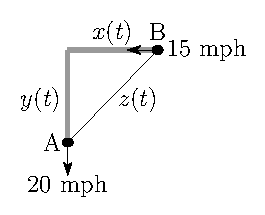
\includegraphics{ship}\end{center}

If $x(t),\ y(t)$ and $z(t)$ are the distances shown, at time
$t$, then
\begin{align*}
x(t)^2+y(t)^2&=z(t)^2
\intertext{Differentiating with respect to $t$,}
2x(t)x'(t)+2y(t)y'(t)&=2z(t)z'(t)\\
x(t)x'(t)+y(t)y'(t)&=z(t)z'(t)
\intertext{At the specified time, $x(t)$ is decreasing, so $x'(t)$ is negative.}
 (300)(-15)+(400)(20) &= \sqrt{300^2+400^2}z'(t)\\
500 z'(t)&=3500\\
z'(t)&=7 \mbox{ mph}
\end{align*}
\end{solution}


%\begin{question}[2015Q]
%Boat $A$ travels north at 30km/h and boat $B$ travels east at 40km/h. These
%boats started from the same point at 12pm. When boat $B$ has traveled 20km, how fast is the distance between boat $A$ and $B$ increasing?
%\end{question}
%\begin{answer} 16 kph
%\end{answer}
%\begin{solution}
%\begin{itemize}
% \item
%We think the start as the origin in the plane. Then, we compute the distance $z(t)$
%between boat A and B at each moment in time as
%\begin{align*}
%z^2(t)&= x(t)^2+y(t)^2,
%\end{align*}
%where $x(t)$ is the position on the $x$-axis of boat B at time $t$
%(measured in hours) and $y(t)$ is the position on the $y$-axis of boat
%A at the same time $t$.
%\item We differentiate the above equation with respect to $t$ and get
%\begin{align*}
%2z \cdot z' &= 2x \cdot x' + 2 y \cdot y',
%\end{align*}
%\item We are told that $x'=40$ and $y'=30$. Further it will take $0.5$ hours
%for boat $B$ to travel $20$km, and in this time boat $A$ will travel
%$15$km.
%\item Alternatively, write $x=40t,y=30t$ to get $t=1/2,
%x'=40,y'=30,y=15$.
%\item At this point $z = \sqrt{x^2+y^2}=\sqrt{40^2+30^2}=50$.
%\item Hence
%\begin{align*}
%  100z' &= 40\cdot(40)+30\cdot(30) = 1600 \\
%  z' &= \frac{1600}{100} =16  \text{km per hour}.
%\end{align*}
%\end{itemize}
%\end{solution}




%\begin{question}
%Child $A$ and Child $B$ are sitting in the same spot. At exactly noon, Child $A$ sees a dog, and runs due east towards it at a steady pace of 1 meter per second. One second later (at one second past noon), Child $B$ sees a spider, and runs due north away from it at a steady pace of 2 meters per second. How fast is the distance between the children increasing at three seconds past noon?
%\end{question}
%\begin{hint} Find an equation that relates the distance between the two children to each child's distance from their starting point.
%\end{hint}
%\begin{answer} $11/5$ meters per second
%\end{answer}
%\begin{solution}
%\begin{center}\begin{tikzpicture}
%\draw[thick, ->] (0,0) node[vertex]{}--(2,0) ;
%\draw (1,-.5) node{$a(t)$};
%\draw[thick, ->] (0,0)--(0,3);
%\draw (-.5,1.5) node{$b(t)$};
%\draw[dashed] (2,0) -- (0,3) node[midway, label= right:$D$]{};
%\end{tikzpicture}\end{center}
%\begin{itemize}
% \item The children start at the same point. Let $a$ be Child $A$'s distance from that point, and let $b$ be Child $B$'s distance from that point. Then we know $\diff{a}{t}=1$ meter per second, and $\diff{b}{t}=2$ meters per second.  Note these rates are both positive.
%
% \item Our units are measured in seconds. Let noon be $t=0$. If $D$ is the distance between the children, we want to know $\diff{D}{t}$ when $t=3$.
%
%\item So, we need an equation relating $a$, $b$, and $D$. Of course this equation is
%\[D^2=a^2+b^2\]
%and we differentiate with respect to $t$:
%\[2D\diff{D}{t} = 2a\diff{a}{t}+2b\diff{b}{t}\]
%
%\item To solve for $\diff{D}{t}$, we need $a$, $b$, and $D$ when $t=3$. Since Child $A$ starts running at $t=0$, $\left.a\right|_{t=3}=1\cdot 3=3$ meters. Since Child $B$ starts running at $t=1$, $\left.b\right|_{t=3}=2(3-1)=4$ meters. Then $\left.D\right|_{t=3}=\sqrt{3^2+4^2}=5$.
%
%\item Now we solve for $\diff{D}{t}$:
%\begin{align*}
%2D\diff{D}{t} &= 2a\diff{a}{t}+2b\diff{b}{t}\\
%2(5)\left.\diff{D}{t}\right|_{t=3} &=2(3)(1)+2(4)(2)\\
%\left.\diff{D}{t}\right|_{t=3}&={\frac{11}{5}} \mbox{ meters per second}
%\end{align*}
%
%\item Equivalently, we can write $a=t$ and $b=2(t-1)$, so $D^2=a^2+b^2=t^2+4(t-1)^2$. Then
%\[2D\diff{D}{t} = 2t+8(t-1)\]
%So
%\[2(5)\left.\diff{D}{t}\right|_{t=3} = 2(3)+8(3-1)=22\]
%hence $\ds\diff{D}{t}={\frac{11}{5}}$ meters per second.
%\end{itemize}
%\end{solution}



\begin{Mquestion}[2015Q]
Two tall sticks are vertically planted into the ground, separated by a distance of $30$ cm. We simultaneously put two snails at the base of each stick. The two snails then begin to climb their respective sticks. The first snail is moving with a speed of $25$ cm per minute, while the second snail is moving with a speed of $15$ cm per minute.
What is the rate of
change of the distance between the two snails when the first snail reaches $100$ cm above the ground?
\end{Mquestion}
\begin{hint}
You'll want to think about the \emph{difference} in height of the two snails.
\end{hint}
\begin{answer}
$8$ cm per minute
\end{answer}
\begin{solution}
\begin{itemize}
 \item
We compute the distance $d(t)$ between the two snails after $t$ minutes as
\begin{align*}
d^2(t)&= 30^2 + (y_1(t)-y_2(t))^2,
\end{align*}
where $y_1(t)$ is the altitude of the first snail, and $y_2(t)$ the altitude of the second snail after $t$ minutes.
\item We differentiate the above equation with respect to $t$ and get
\begin{align*}
2d \cdot d' &= 2 ({y_1}' - {y_2}') (y_1 - y_2)\\
d \cdot d' &=  ({y_1}' - {y_2}') (y_1 - y_2)
\end{align*}
\item We are told that ${y_1}'=25$ and ${y_2}'=15$. It will take $4$ minutes
for the first snail to reach $y_1=100$, and in this time  the second snail will reach
$y_2=60$.
\item At this point $d^2 = 30^2 + (100-60)^2 = 900 + 1600 = 2500$, hence $d = 50$.
\item Therefore
\begin{align*}
50  d' &=  (25 - 15) \times (100 - 60)   \\
  d' &= \frac{400}{50} = 8 \text{ cm per minute}.
\end{align*}
\end{itemize}
\end{solution}



\begin{question}[2015Q]\label{s3.2Pythagoruslast}
A $20$m long extension ladder leaning against a wall starts collapsing in on itself at a
rate of $2$m/s, while the foot of the ladder remains a constant $5$m from the wall.
How fast is the ladder moving down the wall after $3.5$ seconds?
\end{question}
\begin{hint} The length of the ladder is changing.
\end{hint}
\begin{answer}
$-\dfrac{13}{6}$ metres per second
\end{answer}
\begin{solution}
\begin{itemize}
 \item
    If we write $z(t)$ for the length of the ladder at time $t$ and $y(t)$ for the height of the top end of the ladder at time $t$ we have
    \[
        z(t)^2 = 5^2 + y(t)^2.
    \]
\item We differentiate the above equation with respect to $t$ and get
\begin{align*}
2z \cdot z' &= 2y \cdot y',
\end{align*}
\item We are told that $z'(t)=-2$, so $z(3.5)=20-3.5\cdot2 = 13$.
\item At this point $y = \sqrt{z^2-5^2} = \sqrt{169-25} = \sqrt{144} = 12$.
\item Hence
\begin{align*}
  2\cdot 13 \cdot (-2) &= 2 \cdot 12 y' \\
  y' &= -\frac{2\cdot 13}{12} = -\frac{13}{6} \text{ meters per second}.
\end{align*}
\end{itemize}
\end{solution}



%%%%%%%%%%%%%%%%%%
%\subsubsection*{Problems involving similar triangles and other trigonometric tidbits}
%%%%%%%%%%%%%%%%%%
\Instructions{
For Questions \ref{s3.2trianglesfirst} through
\ref{s3.2triangleslast}, look for tricks from trigonometry.}


\begin{Mquestion}\label{s3.2trianglesfirst}
A watering trough has a cross section shaped like an isosceles trapezoid. The trough is 2 metres long, 50 cm high, 1 metre wide at the top, and 60 cm wide at the bottom.
\begin{center}\begin{tikzpicture}
\draw[fill=black!10] (0,0)--(3,0)--(4,2.5)--(-1,2.5)--cycle;
\draw[fill=black!15] (4,2.5)--(7,3.5)--(6,1)--(3,0);
\draw[fill=black!20] (-1,2.5)--(2,3.5)--(7,3.5)--(4,2.5)--cycle;
\draw (2,3.5)--(2.2,2.5);
\draw (1.5,-.5) node{$60$ cm};
\draw (1.5,2) node{$1$ m};
\draw[<->] (-1.5,0)--(-1.5,2.5) node[midway, left]{$50$ cm};
\draw[<->] (-1.1,3)--(1.9,4) node[midway, above]{$2$ m};
\end{tikzpicture}\end{center}
A pig is drinking water from the trough at a rate of 3 litres per minute. When the height of the water is 25 cm, how fast is the height decreasing?
\end{Mquestion}
\begin{hint}
If a  trapezoid has height $h$ and (parallel) bases $b_1$ and $b_2$, then its area is $h\left(\frac{b_1+b_2}{2}\right)$. To figure out how wide the top of the water is when the water is at height $h$, you can cut the trapezoid up into a rectangle and two triangles, and make use of similar triangles.
\end{hint}
\begin{answer} The height of the water is decreasing at
$\dfrac{3}{16}=0.1875~\frac{\mathrm{cm}}{\mathrm{min}}$.
\end{answer}
\begin{solution}
What we're given is $\ds\diff{V}{t}$ (where $V$ is volume of water in the trough, and $t$ is time), and what we are asked for is $\ds\diff{h}{t}$ (where $h$ is the height of the water). So, we need an equation relating $V$ and $h$. First, let's get everything in the same units: centimetres.

\begin{center}\begin{tikzpicture}
\draw[fill=black!10] (0,0)--(3,0)--(4,2.5)--(-1,2.5)--cycle;
\draw[fill=black!15] (4,2.5)--(7,3.5)--(6,1)--(3,0);
\draw[fill=black!20] (-1,2.5)--(2,3.5)--(7,3.5)--(4,2.5)--cycle;
\draw (2,3.5)--(2.2,2.5);
\draw (1.5,-.5) node{$60$ cm};
\draw (1.5,2) node{$100$ cm};
\draw[<->] (-1.5,0)--(-1.5,2.5) node[midway, left]{$50$ cm};
\draw[<->] (-1.1,3)--(1.9,4) node[midway, above, rotate=18]{$200$ cm};
\draw[fill=blue!10] (0,0)--(3,0)--(3.4,1)--(-.4,1)--cycle;
\draw[fill=blue!15](3,0)--(6,1)--(6.4,2)--(3.4,1)--cycle;
\draw[<->, blue] (-.75,0)--(-.75,.9) node[midway, left]{$h$};
\draw[blue] (1.5,.75)node{$w$};
\end{tikzpicture}\end{center}

We can calculate the volume of water in the trough by multiplying the area of its trapezoidal cross section by 200 cm. A  trapezoid with height $h$ and bases $b_1$ and $b_2$ has area $h\left(\frac{b_1+b_2}{2}\right)$. (To see why this is so, draw the trapezoid as a rectangle flanked by two triangles.)
So, using  $w$ as the width of the top of the water (as in the diagram above), the area of the cross section of the water in the trough is
\[A=h\left(\frac{60+w}{2}\right)\]
and therefore the volume of water in the trough is
\[V=100h(60+w)~\text{cm}^3.\]
We need a formula for $w$ in terms of $h$.
If we draw lines straight up from the bottom corners of the trapezoid, we break it into rectangles and triangles.
\begin{center}\begin{tikzpicture}
\draw (0,0)--(3,0)--(4,2.5)--(-1,2.5)--cycle;
\draw[<->, dashed] (0,-.5)--(3,-.5) node[midway, shape=rectangle, fill=white, inner sep=0]{$60$ };
%\draw[<->, dashed, blue] (-.5,1.5)--(3.5,1.5) node[midway, shape=rectangle, fill=white, inner sep=0]{$w$ };
%\draw[<->, dashed](-1,3)-- (4,3) node[midway, shape=rectangle, fill=white, inner sep=0]{$100$ };
\draw[<->, dashed] (-1.5,0)--(-1.5,2.5) node[midway, left]{$50$ };
\draw[fill=blue!10] (0,0)--(3,0)--(3.4,1)--(-.4,1)--cycle;
\draw[<->, blue, dashed] (-.75,0)--(-.75,.9) node[midway, left]{$h$};
\draw[dashed] (0,0)--(0,2.5) (3,0)--(3,2.5);
\draw[blue] (3.25,1.25) node{a};
\draw[<->, dashed] (3,2.75) --(4,2.74)node[midway, shape=rectangle, fill=white, inner sep=0]{$20$};
\end{tikzpicture}\end{center}
 Using similar triangles,
$\dfrac{a}{h}=\dfrac{20}{50}$,
so $a=\dfrac{2}{5}h$. Then
\begin{align*}
w&=60+2a\\&=60+2\left(\frac{2}{5}h\right)=60+\frac{4}{5}h
\intertext{so}
V&=100h(60+w)\\&=100h(120+\frac{4}{5}h)\\&=80h^2+12000h
\intertext{This is the equation we need, relating $V$ and $h$. Differentiating implicitly with respect to $t$:}
\diff{V}{t}
&=2\cdot80h\cdot\diff{h}{t}+12000\diff{h}{t}\\
&=\left(160h+12000\right)\diff{h}{t}
\intertext{We are given that $h=25$ and $\ds\diff{V}{t}=3$ litres per minute. Converting to cubic centimetres, $\ds\diff{V}{t} = -3000$ cubic centimetres per minute. So:}
-3000&=\left(160\cdot25+12000\right)\diff{h}{t}\\
\diff{h}{t}&=-\frac{3}{16}=-.1875~\frac{\mathrm{cm}}{\mathrm{min}}
\end{align*}
So, the water level is dropping at $\dfrac{3}{16}$ centimetres per minute.
\end{solution}





\begin{question}
A tank is 5 metres long, and has a trapezoidal cross section with the dimensions shown below.

\begin{center}\begin{tikzpicture}
\draw (0,0)--(12,0)--(6,5)--(-2,5)--cycle;
\draw[fill=gray!20] (-2,5)--(-1,6)--(7,6)--(13,1)--(12,0)--(6,5)--(-2,5);
\draw (6,5)--(7,6);
\draw[dashed] (0,0)--(0,5) node[midway, right]{$1.25$ m};
\draw[dashed] (6,0)--(6,5);
\draw[decorate, decoration={brace, amplitude=10pt, mirror}] (6,0)--(12,0) node[midway, yshift=-15pt]{3 m};
\draw[decorate, decoration={brace, amplitude=10pt, mirror}] (0,0)--(6,0) node[midway, yshift=-15pt]{3 m};
\draw[decorate, decoration={brace, amplitude=10pt}] (-2,5)--(0,5) node[midway, yshift=15pt]{1 m};
\draw[decorate, decoration={brace, amplitude=10pt, mirror}] (12,0)--(13,1) node[midway, xshift=20pt, yshift=-10 pt]{5 m};
\end{tikzpicture}
\end{center}
A hose is filling the tank up at a rate of one litre per second. How fast is the height of the water increasing when the water is 10 centimetres deep?
\end{question}

\begin{hint}
Be careful with units. One litre is 1000 cm$^3$, which is not the same as $10$ m$^3$.
\end{hint}

\begin{answer}
$\dfrac{1}{29200}$ metres per second (or about 1 centimetre every five minutes)
\end{answer}

\begin{solution}
If $V$ is the volume of the water in the tank, and $t$ is time, then we are given $\ds\diff{V}{t}$. What we want to know is $\ds\diff{h}{t}$, where $h$ is the height of the water in the tank. A reasonable plan is to find an equation relating $V$ and $h$, and differentiate it implicitly with respect to $t$.

Let's be a little careful about units.
The volume of water in the tank is
\[\text{(area of cross section of water)$\times$(length of tank)}\] If we measure these values in metres (area in square metres, length in metres), then the volume is going to be in cubic metres. So, when we differentiate with respect to time, our units will be cubic metres per second. The water is flowing in at one litre per second, or $1000$ cubic centimetres per second. So, we either have to measure our areas and distances in centimetres, or convert litres to cubic metres. We'll do the latter, but both are fine.

 If we imagine one cubic metre as a cube, with each side of length 1 metre, then it's easy to see the volume inside is $(100)^3=10^6$ cubic centimetres: it's the volume of a cube with each side of length 100 cm. Since a litre is $10^3$ cubic centimetres, and a cubic metre is $10^{6}$ cubic centimetres, one litre is $10^{-3}$ cubic metres.
So, \textcolor{red}{$\ds\diff{V}{t}=\frac{1}{10^3}$} cubic metres per second.

Let $h$ be the height of the water (in metres). We can figure out the area of the cross section by breaking it into three pieces: a triangle on the left, a rectangle in the middle, and a trapezoid on the right.

\begin{center}\begin{tikzpicture}
\draw[blue, fill=blue!10] (-.8,2)--(9.6,2)--(12,0)--(0,0)--cycle;
\draw[blue, dashed, <->, ultra thick] (-1,0)--(-1,2) node[midway, left]{$h$};
\draw[blue, dashed, <->, ultra thick] (-1,2.25)--(0,2.25) node[midway, above]{$a$};
\draw[blue, dashed, <->, ultra thick] (6.,2.25)--(9.5,2.25) node[midway, above]{$b$};
\draw (0,0)--(12,0)--(6,5)--(-2,5)--cycle;
\draw[dashed] (0,0)--(0,5);
\draw[dashed, <->, ultra thick] (-2,0)--(-2,5) node[midway, left]{$1.25$ m};
\draw[dashed] (6,0)--(6,5);
\draw[decorate, decoration={brace, amplitude=10pt, mirror}] (6,0)--(12,0) node[midway, yshift=-15pt]{3 m};
\draw[decorate, decoration={brace, amplitude=10pt, mirror}] (0,0)--(6,0) node[midway, yshift=-15pt]{3 m};
\draw[decorate, decoration={brace, amplitude=10pt}] (-2,5)--(0,5) node[midway, yshift=15pt]{1 m};
\end{tikzpicture}
\end{center}

\begin{itemize}
\item The triangle on the left has height $h$ metres. Let its base be $a$ metres.
It forms a similar triangle with the triangle whose height is 1.25 metres and width is 1 metre, so:
\begin{align*}
\frac{a}{h}&=\frac{1}{1.25}\\
a&=\frac{4}{5}h
\intertext{So, the area of the triangle on the left is}
\frac{1}{2}ah&=\frac{2}{5}h^2
\end{align*}

\item The rectangle in the middle has length 3 metres and height $h$ metres, so its area is $3h$ square metres.

\item The trapezoid on the right is a portion of a triangle with base 3 metres and height 1.25 metres. So, its area is
\begin{align*}&~\underbrace{\left(\frac{1}{2}(3)(1.25)\right) }_{\mbox{area of big triangle}}- \underbrace{\left(\frac{1}{2}(b)(1.25-h)\right)}_{\mbox{area of little triangle}}
\intertext{The little triangle (of base $b$ and height $1.25-h$) is formed by the \emph{air} on the right side of the tank. It is a similar triangle to the triangle of base 3 and height 1.25, so}
\frac{b}{1.25-h}&=\frac{3}{1.25}\\
b&=\frac{3}{1.25}(1.25-h)
\intertext{So, the area of the trapezoid on the right is}
&~\frac{1}{2}(3)(1.25)-\frac{1}{2}\left(\frac{3}{1.25}\right)\left(1.25-h\right)(1.25-h)\\
&=3h-\frac{6}{5}h^2
\end{align*}
\end{itemize}

So, the area $A$ of the cross section of the water is
\begin{align*}
A&=\underbrace{\frac{2}{5}h^2}_{\mbox{triangle}}+
\underbrace{3h}_{\mbox{rectangle}}+
\underbrace{3h-\frac{6}{5}h^2}_{\mbox{trapezoid}}\\
&=6h-\frac{4}{5}h^2
\intertext{So, the volume of water is}
V&=5\left(6h-\frac{4}{5}h^2\right)=30h-4h^2
\intertext{Differentiating with respect to time, $t$:}
\diff{V}{t}&=30\diff{h}{t}-8h\diff{h}{t}
\intertext{When $h=\dfrac{1}{10}$ metre, and $\ds\diff{V}{t}=\frac{1}{10^3}$ cubic metres per second,}
\frac{1}{10^3}&=30\diff{h}{t}-8\left(\frac{1}{10}\right)\diff{h}{t}\\
\diff{h}{t}&=\frac{1}{29200} \mbox{ metres per second}
\end{align*}
This is about 1 centimetre every five minutes. You might want a bigger hose.
\end{solution}


\begin{question}
A rocket is blasting off, 2 kilometres away from you. You and the rocket start at the same height. The height of the rocket in kilometres, $t$ hours after liftoff, is given by
\[h(t)=61750t^2\]
How fast (in radians per second) is your line of sight rotating to keep looking at the rocket, one minute after liftoff?
\end{question}
\begin{hint}
You, the rocket, and the rocket's original position form a right triangle.
\end{hint}
\begin{answer}
$\left(\dfrac{2}{\left(\frac{1235}{72}\right)^2+4}\right)\left(\dfrac{6175}{3}\right)\approx
13.8~\frac{\mathrm{rad}}{\mathrm{hour}} \approx 0.0038~\frac{\mathrm{rad}}{\mathrm{sec}}$
\end{answer}
\begin{solution}
Let $\theta$ be the angle of your head, where $\theta=0$  means you are looking straight ahead, and $\theta=\dfrac{\pi}{2}$ means you are looking straight up.
We are interested in $\ds\diff{\theta}{t}$, but we only have information about $h$. So, a reasonable plan is to find an equation relating $h$ and $\theta$, and differentiate with respect to time.

\begin{center}\begin{tikzpicture}
\draw (1.5,0)--(0,0)--(1,1);
\draw (1,0) arc(0:45:1cm);
\draw (.8,.4) node[shape=ellipse, minimum height=.4cm, minimum width=0.2cm, draw, fill, inner sep=0, rotate=20]{};
\draw[dashed] (4,.4)--(.8,.4)--(4,3);
\draw (1.6,.4) arc(0:37:.8) ;
\draw (1.75,0.75) node{$\theta$};
\draw (4.5,2.5)--(4.5,3.5)--(4.75,4)--(5,3.5)--(5,2.5)--cycle;
\draw[yshift=-2.6cm] (4.5,2.5)--(4.5,3.5)--(4.75,4)--(5,3.5)--(5,2.5)--cycle;
\draw [thick, ->] (4.75,1.75)--(4.75,2.25);
\end{tikzpicture}\end{center}

The right triangle formed by you, the rocket, and the rocket's original position has adjacent side (to $\theta$) length 2km, and opposite side (to $\theta$) length $h(t)$ kilometres, so
\begin{align*}
\tan\theta&=\frac{h}{2}
\intertext{Differentiating with respect to $t$:}
\sec^2\theta \cdot \diff{\theta}{t}&=\frac{1}{2}\diff{h}{t}\\
\diff{\theta}{t}&=\frac{1}{2}\cos^2\theta\cdot\diff{h}{t}
\end{align*}
We know $\tan\theta= \frac{h}{2}$. We draw a right triangle with angle $\theta$ (filling in the sides using SOH~CAH~TOA and the Pythagorean theorem) to figure out $\cos\theta$:
\begin{center}\begin{tikzpicture}
\draw (0,0)--(4,0)--(4,3)--cycle;
\draw (.75,.2) node{$\theta$};
\draw (2,0) node[below]{2};
\draw (4.25,1.5) node{$h$};
\draw (2,2) node[rotate=37]{$\sqrt{h^2+4}$};
\end{tikzpicture}\end{center}
Using the triangle, $\cos\theta = \dfrac{2}{\sqrt{h^2+4}}$, so
\begin{align*}
\diff{\theta}{t}&=\frac{1}{2}\left(\frac{2}{\sqrt{h^2+4}}\right)^2\cdot\diff{h}{t}\\
&=\left(\frac{2}{h^2+4}\right)\diff{h}{t}
\intertext{So, the quantities we need to know one minute after liftoff (that is, when $t = \dfrac{1}{60}$) are $h\left(\dfrac{1}{60}\right)$ and $\ds\diff{h}{t}\left(\frac{1}{60}\right)$. Recall $h(t)=61750t^2$.}
h\left(\frac{1}{60}\right)&=\frac{61750}{3600}=\frac{1235}{72}\\
\diff{h}{t}&=2(61750)t\\
\diff{h}{t}\left(\frac{1}{60}\right)&=\frac{2(61750)}{60}=\frac{6175}{3}
\intertext{Returning to the equation
$\ds\diff{\theta}{t}=\left(\dfrac{2}{h^2+4}\right)\ds\diff{h}{t}
$:}
\diff{\theta}{t}\left(\frac{1}{60}\right)&=\left(\frac{2}{\left(\frac{1235}{72}\right)^2+4}\right)\left(\frac{6175}{3}
\right)\approx 13.8~\frac{\mathrm{rad}}{\mathrm{hour}}\approx 0.0038~\frac{\mathrm{rad}}{\mathrm{sec}}
\end{align*}

\end{solution}



\begin{Mquestion}[1998H]
A high speed train is traveling at 2 km/min
along a straight track. The train is moving away from a movie camera which
is located 0.5 km from the track.
\begin{enumerate}[(a)]
\item\label{s3.2train1} How fast is the distance between the train and the camera
increasing when they are 1.3 km apart?
\item\label{s3.2train2}  Assuming that the camera is always pointed at the train,
how fast (in radians per min) is the camera rotating when the train and the
camera are 1.3 km apart?
\end{enumerate}
\end{Mquestion}
\begin{hint} Your picture should be a triangle.
\end{hint}
\begin{answer}
\eqref{s3.2train1} $\dfrac{24}{13}\approx 1.85$ km/min \qquad
\eqref{s3.2train2} about $.592$ radians/min
\end{answer}
\begin{solution}
\eqref{s3.2train1}
Let $x(t)$ be the distance of the train along the track at
time $t$, measured
from the point on the track nearest the camera. Let $z(t)$ be the distance
from the camera to the train at time $t$.

\begin{center}
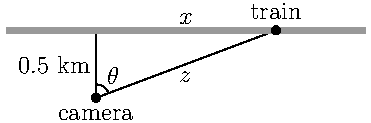
\includegraphics{train2}
\end{center}

Then \textcolor{red}{$x'(t)=2$} and at the time
in question, \textcolor{red}{$z(t)=1.3$} km and $\textcolor{red}{x(t)}=\sqrt{1.3^2-0.5^2}=\textcolor{red}{1.2}$ km. So
\begin{align*}
z(t)^2&=x(t)^2+0.5^2\\
 2z(t)z'(t)&=2x(t)x'(t)\\
 2\times 1.3z'(t)&=2\times 1.2\times 2\\
\color{red}z'(t)&\textcolor{red}{=\frac{2\times 1.2}{1.3}}\approx1.85 \mbox{ km/min}
\end{align*}

\eqref{s3.2train2}
Let $\theta(t)$ be the angle shown at time $t$. Then
\begin{align*}
\sin\left(\theta(t)\right)&=\frac{x(t)}{z(t)}\intertext{Differentiating with respect to $t$:}
\theta'(t)\cos\left(\theta(t)\right)
&=\frac{x'(t)z(t)-x(t)z'(t)}{z(t)^2}\\
\theta'(t)&=\frac{x'(t)z(t)-x(t)z'(t)}{z(t)^2\cos\left(\theta(t)\right)}
\intertext{From our diagram, we see $\cos\left(\theta(t)\right)=\dfrac{0.5}{z(t)}$, so:}
&=2\frac{x'(t)z(t)-x(t)z'(t)}{z(t)}
\intertext{Substituting in $x'(t)=2$, $z(t)=1.3$, $x(t)=1.2$, and $z'(t)=\dfrac{2\times1.2}{1.3}$:}
\theta'(t)
&=2\frac{2\times 1.3-1.2\times\frac{2\times 1.2}{1.3}}{1.3}
\approx .592  \mbox{ radians/min}
\end{align*}
\end{solution}


\begin{Mquestion}[1996D]
A ball is dropped from a height of $49$ metres above the ground. The
height of the ball at time $t$ is $h(t)=49-4.9 t^2$ m. A light, which is
also $49$ m above the ground, is $10$ m to the left of the ball's original
position. As the ball descends, the shadow of the ball caused by the light
moves across the ground. How fast is the shadow moving one second after
the ball is dropped?

\begin{center}
%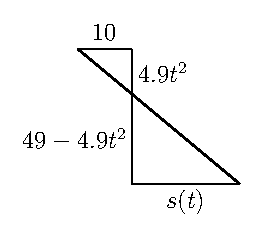
\includegraphics{ballShadow}
\begin{tikzpicture}
\draw[red, dashed] (0,3)--(6,0);
\draw[red] (0,3)--(2,3) node[midway, above]{10};
\draw[ultra thick] (0,0)--(0,3) node[midway, left]{49} node[opendot, label= left:{light}]{};
\draw[red, thick,<-] (2,1.5)--(2,3) ;
\draw[red, thick] (2,1.5)--(2,0) ;%node[above right]{ball};
\draw (2,2) node[shape=circle, minimum size=3mm, draw, fill=white, label=right:{$h(t)=49-4.9t^2$}]{};
\draw (1.75,2) node[left]{ball};
\draw[red] (2,0) -- (6,0) node[midway, below]{$s(t)$};
\end{tikzpicture}\end{center}
\end{Mquestion}
\begin{hint} In the diagram, find two similar triangles.
\end{hint}
\begin{answer} 200 m/s to the left
\end{answer}
\begin{solution}
In the diagram, there are two right triangles: one formed by the light, the ball, and the ball's original position, and one formed by the ball, the tip of its shadow, and the ball's eventual position on the ground. The two angles marked below have the same measure, $\alpha$. (Whenever two straignt lines cross, the opposite angles formed have the same measure.)

\begin{center}
\begin{tikzpicture}
\draw[red, dashed] (0,3)--(6,0);
\draw[red] (0,3)--(2,3) node[midway, above]{10};
\draw[dashed, <->, thick](0,0)--(0,2) node[midway,left]{$49-4.9t^2$};
\draw[dashed, <->, thick](-1,2)--(-1,3) node[midway,left]{$4.9t^2$};
\draw[red, thick] (2,0)--(2,3) ;
\draw[red] (2,0) -- (6,0) node[midway, below]{$s(t)$};
\draw (2,2.25) node[above left]{$\alpha$};
\draw (2,1.75) node[below right]{$\alpha$};
\draw (2,2.25) arc(90:145:.25);
\draw (2,1.75) arc(-90:-35:.25);
\end{tikzpicture}\end{center}

Since the two triangles share two angles in common (a right angle, and an angle of measure $\alpha$), they are similar triangles.
Let's call $s(t)$ the distance from the shadow to the point
on the ground directly underneath the ball. Since the triangles are similar,
\begin{align*}
\frac{4.9 t^2}{10}&=\frac{49-4.9 t^2}{s(t)}\\
 s(t)&=10\frac{49-4.9 t^2}{4.9 t^2}=\frac{100}{t^2}-10\\
 s'(t)&=-2\frac{100}{t^3}
\end{align*}
When $t=1$, $s'(1)=-200$ m/sec. That is, {the shadow is moving to the
left at $200$ m/sec.}
\end{solution}

\begin{question}\label{s3.2triangleslast}
A clock has a minute hand that is 10 cm long, and an hour hand that is 5 cm long.
Let $D$ be the distance between the tips of the two hands. How fast is $D$ decreasing at 4:00?
\begin{center}\begin{tikzpicture}
\draw[ultra thick] node[shape=circle, minimum size=5cm, draw]{};
\draw node[vertex]{};
\draw[very thick, ->] (0,0)--(0,2) node(m){};
\draw[very thick, ->] (0,0)--(0.866,-.5) node(h){};
\draw[dashed, thick, red] (m)--(h) node[midway, right]{$D$};
\foreach \x in {0,...,11}{
	\draw (0,0)+(30*\x:2.1cm) node(o\x){};
	\draw (0,0)+(30*\x:2.75cm) node(i\x){};
	\draw (o\x)--(i\x);}
\end{tikzpicture}\end{center}
\end{question}
\begin{hint}
Let $\theta$ be the angle between the two hands. Using the Law of Cosines, you can get an expression for $D$ in terms of $\theta$.  To find $\ds\diff{\theta}{t}$, use what you know about how fast clock hands move.
\end{hint}
\begin{answer}
$\dfrac{55\sqrt{21}\pi}{42}\approx 19$ centimetres per hour.
\end{answer}
\begin{solution}
Let $\theta$ be the angle between the two hands.
\begin{center}\begin{tikzpicture}
\draw[ultra thick] node[shape=circle, minimum size=5cm, draw]{};
\draw node[vertex]{};
\draw[very thick, ->] (0,0)--(0,2) node(m){};
\draw[very thick, ->] (0,0)--(0.866,-.5) node(h){};
\draw[dashed, thick, red] (m)--(h) node[midway, right]{$D$};
\draw[red] (.25,.25) node{$\theta$};
\draw (.25,-.5) node[rotate=-30]{5cm};
\draw (-.35,1) node[rotate=90]{10cm};
\end{tikzpicture}\end{center}
The Law of Cosines (Appendix~\ref*{app cosine law}%B.4.11
) tells us that
\begin{align*}
D^2&=5^2+10^2-2\cdot5\cdot10\cdot\cos\theta\\
D^2&=125-100\cos\theta\intertext{Differentiating with respect to time $t$,}
2D\diff{D}{t}&=100\sin\theta\cdot\diff{\theta}{t}\\
\end{align*}
Our tasks now are to find  $D$, $\theta$ and $\ds\diff{\theta}{t}$ when the time is 4:00.
At 4:00, the minute hand is straight up, and the hour hand is $\dfrac{4}{12}=\dfrac{1}{3}$ of the way around the clock, so \textcolor{red}{$\theta = \dfrac{1}{3}(2\pi)=\dfrac{2\pi}{3}$} at 4:00. Then
$D^2=125-100\cos\left(\frac{2\pi}{3}\right)=125-100\left(-\frac{1}{2}\right)=175$, so
\textcolor{red}{$D=\sqrt{175}=5\sqrt{7}$} at 4:00.

To calculate $\ds\diff{\theta}{t}$, remember that both hands are moving. The hour hand makes a full rotation every 12 hours, so its rotational speed is $\dfrac{2\pi}{12}=\dfrac{\pi}{6}$ radians per hour. The hour hand is being chased by the minute hand. The minute hand makes a full rotation every hour, so its rotational speed is $\dfrac{2\pi}{1}=2\pi$ radians per hour. Therefore, the angle $\theta$ \emph{between} the two hands is changing at a rate of
\[\color{red}\ds\diff{\theta}{t}=-\left(2\pi-\dfrac{\pi}{6}\right)=\dfrac{-11\pi}{6}~~\frac{\mathrm{rad}}{\mathrm{hr}}.\]

Now, we plug in $D$, $\theta$, and $\ds\diff{\theta}{t}$ to find $\ds\diff{D}{t}$:
\begin{align*}
2D\diff{D}{t}&=100\sin\theta\cdot\diff{\theta}{t}\\
2\left(5\sqrt{7}\right)\diff{D}{t}&=100\sin\left(\frac{2\pi}{3}\right)\left(\frac{-11\pi}{6}\right)\\
10\sqrt{7}\diff{D}{t}&=
100\left(\frac{\sqrt3}{2}\right)\left(\frac{-11\pi}{6}\right)
=-\frac{275\pi}{\sqrt3}\\
\diff{D}{t}&=\frac{-55\sqrt{21}\pi}{42}  ~~\frac{\mathrm{cm}}{\mathrm{hr}}
\end{align*}
So $D$ is decreasing at $\dfrac{55\sqrt{21}\pi}{42} \approx 19$ centimetres per hour. \end{solution}


%%%%%%%%%%%%%%%%%%
%\subsubsection*{Problems that use formulas for volume or area}
%%%%%%%%%%%%%%%%%%
\Instructions{For Questions \ref{s3.2annulus} through \ref{s3.2formulaslast}, you'll need to know formulas for volume or area.}

\begin{question}[2006H]\label{s3.2annulus}
Find the rate of change of the area of the annulus
$\{ (x, y)~:~ r^2 \le x^2 + y^2 \le R^2 \}$.
(i.e. the points inside the circle of radius $R$ but outside the circle
of radius $r$) if \\$R = 3 ~\mathrm{cm}$, $r = 1~\mathrm{cm}$, $\ds\diff{R}{t} = 2~\frac{\mathrm{cm}}{\mathrm{s}}$, and $\ds\diff{r}{t} = 7~\frac{\mathrm{cm}}{\mathrm{s}}$.
\begin{center}\begin{tikzpicture}
\draw[thick] node[shape=circle, draw, minimum size=5cm, inner sep=0, fill=gray!20]{};
\draw[thick] node[shape=circle, draw, minimum size=2cm, inner sep=0, fill=white]{};
\draw node[vertex]{};
\draw (0,0)--(2.5,0) node[midway,above]{$R$};
\draw (0,-1)--(0,0) node[midway, left]{$r$};
\end{tikzpicture}\end{center}
\end{question}
\begin{hint}
The area in the annulus is the area of the outer circle minus the area of the inner circle.
\end{hint}
\begin{answer}
$\ds\diff{A}{t}=-2\pi~\dfrac{\mathrm{cm}^2}{\mathrm{s}}$
\end{answer}
\begin{solution}
The area at time $t$ is the area of the outer circle minus the area of the inner circle:\begin{align*}A(t)&=\pi\big(R(t)^2-r(t)^2\big)\\
\mbox{So, }~~A'(t)&=2\pi\big(R(t)R'(t)-r(t)r'(t)\big)
\intertext{Plugging in the given data,}
A'&=2\pi\big(3\cdot 2-1\cdot 7\big)=-2\pi
\end{align*}
So the area is \emph{shrinking} at a rate of $2\pi~\dfrac{\mathrm{cm}^2}{\mathrm{s}}$.
\end{solution}



\begin{question}
Two spheres are centred at the same point. The radius $R$ of the bigger sphere at time $t$ is given by $R(t)=10+2t$, while the radius $r$ of the smaller sphere is given by $r(t)=6t$, $t \ge 0$. How fast is the volume between the spheres (inside the big sphere and outside the small sphere) changing when the bigger sphere has a radius twice as large as the smaller?
\end{question}
\begin{hint}
The volume of a sphere with radius $R$ is $\dfrac{4}{3}\pi r^3$.
\end{hint}
\begin{answer}
$288$ cubic units per unit time
\end{answer}
\begin{solution}
The volume between the spheres, while the little one is inside the big one, is
\[V=\frac{4}{3}\pi R^3 - \frac{4}{3}\pi r^3\]
Differentiating implicitly with respect to $t$:
\[\diff{V}{t}=4\pi R^2\diff{R}{t}-4\pi r^2\diff{r}{t}\]

We differentiate $R=10+2t$ and $r=6t$ to find $\ds\diff{R}{t}=2$ and $\ds\diff{r}{t}=6$. When $R=2r$, $10+2t=2(6t)$, so $t=1$. When $t=1$, $R=12$ and $r=6$. So:
\[\diff{V}{t}=4\pi\left(12^2\right)(2)-4\pi\left(6^2\right)(6)=288\pi\]
So the volume between the two spheres is increasing at 288 cubic units per unit time.

Remark: when the radius of the inner sphere increases, we are ``subtracting" more area. Since the radius of the inner sphere grows faster than the radius of the outer sphere, we might expect the area between the spheres to be decreasing. Although the radius of the outer sphere grows more slowly, a small increase in the radius of the outer sphere results in a larger change in volume than the same increase in the radius of the inner sphere. So, a result showing that the volume between the spheres is increasing is not unreasonable.
\end{solution}



\begin{Mquestion}
You attach two sticks together at their ends, and stick the other ends in the mud. One stick is 150 cm long, and the other is 200 cm.
\begin{center}\begin{tikzpicture}
\draw[ultra thick, brown!50] (-3,0)--(5,0);
\draw[ultra thick] (-3,0)--(0,2)node[midway, above, rotate=31]{150 cm};
\draw[ultra thick] (0,2)--(5,0)node[midway, above, rotate=-22]{200 cm};
\draw[dashed, <->] (-4,0)--(-4,2) node[midway, left]{1.4 m};
\end{tikzpicture}\end{center}
The structure starts out being 1.4 metres high at its peak, but the sticks slide, and the height decreases at a constant rate of three centimetres per minute. How quickly is the area of the triangle (formed by the two sticks and the level ground) changing when the height of the structure is 120 cm?
\end{Mquestion}
\begin{hint}
The area of a triangle is half its base times its height. To find the base, split the triangle into two right triangles.
\end{hint}
\begin{answer}
0 square centimetres per minute
\end{answer}
\begin{solution}
We know something about the rate of change of the  height $h$ of the triangle, and we want to know something about the rate of change of its area, $A$. A reasonable plan is to find an equation relating $A$ and $h$, and differentiate implicitly with respect to $t$.
The area of a triangle with height $h$ and base $b$ is
\begin{align*}
A&=\frac{1}{2}bh\intertext{Note, $b$ will change with time as well as $h$. So, differentiating with respect to time, $t$:}
\diff{A}{t}&=\frac{1}{2}\left(\diff{b}{t}\cdot h+b\cdot\diff{h}{t}\right)
\end{align*}
We are given $\diff{h}{t}$ and $h$, but those $b$'s are a mystery. We need to relate them to $h$. We can do this by breaking our triangle into  two right triangles and using the Pythagorean Theorem:

\begin{center}\begin{tikzpicture}
\draw[ultra thick, brown!50] (-3,0)--(5,0);
\draw[ultra thick] (-3,0)--(0,2)node[midway, above, rotate=31]{150 cm};
\draw[ultra thick] (0,2)--(5,0)node[midway, above, rotate=-22]{200 cm};
\draw[dashed] (0,0)--(0,2) node[midway, left]{$h$};
\draw[decorate, decoration={brace, mirror, amplitude=10pt}] (-3,0)--(0,0) node[midway,below,yshift=-10pt]{$\sqrt{150^2-h^2}$};
\draw[decorate, decoration={brace, mirror, amplitude=10pt}] (0,0)--(5,0) node[midway,below,yshift=-10pt]{$\sqrt{200^2-h^2}$};
\end{tikzpicture}\end{center}

So, the base of the triangle is
\begin{align*}b&=\sqrt{150^2-h^2}+\sqrt{200^2-h^2}
\intertext{Differentiating with respect to $t$:}
\diff{b}{t}&=\frac{-2h\diff{h}{t}}{2\sqrt{150^2-h^2}}+
\frac{-2h\diff{h}{t}}{2\sqrt{200^2-h^2}}\\
&=\frac{-h\diff{h}{t}}{\sqrt{150^2-h^2}}+
\frac{-h\diff{h}{t}}{\sqrt{200^2-h^2}}\intertext{Using $\ds\diff{h}{t}=-3$ centimetres per minute:}
\diff{b}{t}&=\frac{3h}{\sqrt{150^2-h^2}}+
\frac{3h}{\sqrt{200^2-h^2}}
\intertext{When $h=120$, $\sqrt{150^2-h^2}=90$ and $\sqrt{200^2-h^2}=160$. So, at this moment in time:}
b&=90+160=250\\
\diff{b}{t}&=\frac{3(120)}{90}+\frac{3(120)}{160}
=
4+\frac{9}{4}=\frac{25}{4}
\intertext{We return to our equation relating the derivatives of $A$, $b$, and $h$.}
\diff{A}{t}&=\frac{1}{2}\left(\diff{b}{t}\cdot h + b \cdot \diff{h}{t}\right)
\intertext{When $h=120$ cm, $b=250$, $\ds\diff{h}{t}=-3$, and $\ds\diff{b}{t}=\dfrac{25}{4}$:}
\diff{A}{t}&=\frac{1}{2}\left(\frac{25}{4}(120)+250(-3)\right)\\
&=0
\end{align*}

Remark: What does it mean that $\left.\ds\diff{A}{t}\right|_{h=120}=0$? Certainly, as the height changes, the area changes as well. As the height sinks to 120 cm, the area is increasing, but after it sinks \emph{past} 120 cm, the area is \emph{decreasing}. So, at the instant when the height is exactly 120 cm, the area is neither increasing nor decreasing: it is at a local maximum. You'll learn more about this kind of problem in Section~\ref*{sec optimise}.
\end{solution}




\begin{question}\label{s3.2segment}
The circular lid of a salt shaker has radius 8. There is a cut-out to allow the salt to pour out of the lid, and a door that rotates around to cover the cut-out. The door is a quarter-circle of radius 7 cm. The cut-out has the shape of a quarter-annulus with outer radius 6 cm and inner radius 1 cm.
If the uncovered area of the cut-out is $A$ cm$^2$, then the salt flows out at $\frac{1}{5}A$ cm$^3$ per second.

\begin{center}
\begin{tikzpicture}
\draw node[shape=circle, minimum size=4cm, fill=orange!20,draw]{};
\draw[fill=white] (.5,0)--(1.5,0) arc(0:90:1.5cm)--(0,.5) arc(90:0:.5cm);
\draw[fill=orange!40] (0,0)--(0,-1.75) arc(-90:-180:1.75cm)--(0,0);
\draw[fill=orange!50] node[shape=circle, minimum size=1mm, draw, fill]{};
\draw (0,-3) node{salt shaker lid};
\draw (0,-3.5) node{cut-out uncovered};
\end{tikzpicture}\hspace{2cm}
%\begin{tikzpicture}
%\draw node[shape=circle, minimum size=4cm, fill=orange!20,draw]{};
%\draw[fill=white] (.5,0)--(1.5,0) arc(0:90:1.5cm)--(0,.5) arc(90:0:.5cm);
%\draw[fill=orange!40] (.5,0)--(1.5,0) arc(0:45:1.5cm)--(.35,.35) arc(45:0:.5cm);
%\draw[orange!75] node[shape=circle, minimum size=1mm, draw]{};
%\draw (0,-3) node{\textcolor{blue}{bottom} view of lid};
%\draw (0,-3.5) node{door half open: $\theta=\frac{\pi}{4}$};
%\end{tikzpicture}\hspace{2cm}
\begin{tikzpicture}
\draw node[shape=circle, minimum size=4cm, fill=orange!20,draw]{};
\draw[fill=white] (.5,0)--(1.5,0) arc(0:90:1.5cm)--(0,.5) arc(90:0:.5cm);
\draw[fill=orange!40] (0,0)--(1.24,-1.24) arc(-45:45:1.75cm)--(0,0);
\draw[fill=orange!50] node[shape=circle, minimum size=1mm, draw, fill]{};
\draw[dashed, gray!75] (1.5,0) arc(0:45:1.5cm) (.35,.35) arc(45:0:.5cm)--(1.5,0);
\draw (0,-3) node{salt shaker lid};
\draw (0,-3.5) node{cut-out partially covered};
\end{tikzpicture}
\end{center}
Recall: an annulus is the set of points inside one circle and outside another,  like a flat doughnut (see Question~\ref{s3.2annulus}).

\begin{center}
\begin{tikzpicture}
\draw (0,0) node[shape=circle, minimum size=3cm, draw, fill=gray!20]{};
\draw (0,0) node[shape=circle, minimum size=1cm, draw, fill=white]{};
\draw (0,-2) node{annulus};
\end{tikzpicture}
\hspace{2cm}
\begin{tikzpicture}
\draw[fill=gray!20] (.5,0) arc(0:90:.5cm)--(0,1.5) arc(90:0:1.5cm)--cycle;
\draw[gray!50, dashed] (.5,0) arc(0:-270:.5cm) (0,1.5) arc(90:-270:1.5cm);
\draw (0,-2) node{quarter annulus};
\end{tikzpicture}
\end{center}

While pouring out salt, you spin the door around the lid at a constant rate of $\frac{\pi}{6}$ radians per second, covering more and more of the cut-out. When exactly half of the cut-out is covered, how fast is the flow of salt changing?
\end{question}
\begin{hint}
The easiest way to figure out the area of the sector of an annulus (or a circle) is to
figure out the area of the entire annulus, then multiply by what proportion of the entire annulus the sector is. For example, if your sector is $\frac{1}{10}$ of the entire annulus, then its area is $\frac{1}{10}$ of the area of the entire annulus. (See Section~\ref*{app rad arc sec} %A.4
to  see how this works out for circles.)
\end{hint}
\begin{answer}
$-\dfrac{7\pi}{12}\approx -1.8~\dfrac{\mathrm{cm}^3}{\mathrm{sec}^2}$
\end{answer}
\begin{solution}
Let $S$ be the flow of salt (in cubic centimetres per second). We want to know $\ds\diff{S}{t}$: how fast the flow is changing at time $t$. We are given an equation for $S$:
\[S=\frac{1}{5}A\]
where $A$ is the uncovered area of the cut-out. So,
\[\diff{S}{t}=\frac{1}{5}\diff{A}{t}\]
If we can find $\ds\diff{A}{t}$, then we can find $\ds\diff{S}{t}$.
We are given information about how quickly the door is rotating. If we let $\theta$ be the angle made by the leading edge of the door and the far edge of the cut-out (shown below), then $\ds\diff{\theta}{t}=-\dfrac{\pi}{6}$ radians per second. (Since the door is covering more and more of the cut-out, $\theta$ is getting smaller, so $\ds\diff{\theta}{t}$ is negative.)

\begin{center}
\begin{tikzpicture}
\draw node[shape=circle, minimum size=4cm, fill=orange!20,draw]{};
\draw[fill=white] (.5,0)--(1.5,0) arc(0:90:1.5cm)--(0,.5) arc(90:0:.5cm);
\draw[fill=orange!40] (0,0)--(1.24,-1.24) arc(-45:45:1.75cm)--(0,0);
\draw[fill=orange!50] node[shape=circle, minimum size=1mm, draw, fill]{};
\draw[dashed, gray!75] (1.5,0) arc(0:45:1.5cm) (.35,.35) arc(45:0:.5cm)--(1.5,0);
\draw[thick, red] (0,0)-- (0,2.5) node[right, rotate=90]{edge of cut-out};
\draw[thick, red] (0,0)--(1.7,1.77) node[right, rotate=45]{edge of door};
\draw[red] (.25,.75) node{$\theta$};
\end{tikzpicture}
\end{center}

Since we know $\ds\diff{\theta}{t}$, and we want to know $\ds\diff{A}{t}$ (in order to get $\ds\diff{S}{t}$), it is reasonable to look for an equation relating $A$ and $\theta$, and differentiate it implicitly with respect to $t$ to get an equation relating $\ds\diff{A}{t}$ and $\ds\diff{\theta}{t}$.

The area of an annulus with outer radius 6 cm and inner radius 1 cm is
$\pi\cdot 6^2-\pi\cdot1^2=35\pi$ square centimetres.
A sector of that same annulus with angle $\theta$ has area $\left(\frac{\theta}{2\pi}\right)(35\pi)$, since $\frac{\theta}{2\pi}$ is the ratio of the sector to the entire annulus. (For example, if $\theta=\pi$, then the sector is  \emph{half} of the entire annulus, so its area is $(1/2)35\pi$.)

So, when $0 \leq \theta \leq \frac{\pi}{2}$, the area of the cutout that is open is
\begin{align*}
A&=\frac{\theta}{2\pi}(35\pi)=\frac{35}{2}\theta
\intertext{This is the formula we wanted, relating $A$ and $\theta$. Differentiating with respect to $t$,}
\diff{A}{t}&=\frac{35}{2}\diff{\theta}{t}=\frac{35}{2}\left(-\frac{\pi}{6}\right)=-\frac{35\pi}{12}
\intertext{Since $\ds\diff{S}{t}=\frac{1}{5}\ds\diff{A}{t}$,}
\diff{S}{t}&=-\frac{1}{5}\frac{35\pi}{12}=-\frac{7\pi}{12}\approx -1.8~\frac{\mathrm{cm}^3}{\mathrm{sec}^2}
\end{align*}

Remark: the change in flow of salt is constant while the door covers more and more of the cut-out, so we never used the fact that precisely half of the cut-out was open. We also never used the radius of the lid, which is immaterial to the flow of salt.
\end{solution}


\begin{Mquestion}
A cylindrical sewer pipe with radius 1 metre has a vertical rectangular door that slides  in front of it to block the flow of water, as shown below. If the uncovered area of the pipe is $A$ m$^2$, then the flow of water through the pipe is $\frac{1}{5}A$ cubic metres per second.

The door slides over the pipe, moving vertically at a rate of 1 centimetre per second. How fast is the flow of water changing when the door covers the top 25 centimetres of the pipe?

\begin{center}\begin{tikzpicture}
\draw (-3,0) arc(180:360:3cm);
\draw[fill=gray!50] (-4,0) rectangle (4,4);
\draw[dashed] (3,0) arc(0:180:3cm);
\draw[->, ultra thick, gray] (-4.5,3)--(-4.5,1);
\end{tikzpicture}\end{center}
\end{Mquestion}
\begin{hint}
Think about the ways in which this problem is similar to and different from
Example~\ref*{eg:fuel}
and Question~\ref{s3.2segment}.
\end{hint}
\begin{answer}
The flow is decreasing at a rate of $\dfrac{\sqrt{7}}{1000}~\dfrac{\mathrm{m}^3}{\mathrm{sec}^2}$.
\end{answer}
\begin{solution}
Let $F$ be the flow of water through the pipe, so $F=\dfrac{1}{5}A$. We want to know $\ds\diff{F}{t}$, so differentiating implicitly with respect to $t$, we find
\[\ds\diff{F}{t}=\frac{1}{5}\ds\diff{A}{t}.\]
If we can find $\ds\diff{A}{t}$, then we can find $\ds\diff{F}{t}$. We know something about the shape of the uncovered area of the pipe; a reasonable plan is to find an equation relating the height of the door with the uncovered area of the pipe. Let $h$ be the distance from the top of the pipe to the bottom of the door, measured in metres.

\begin{center}\begin{tikzpicture}
\draw[gray, fill=gray!70] (2.65,3) arc(49:132:4cm) --cycle;
\draw node[shape=circle, minimum size=8cm, draw]{};
\draw[dashed] (2.65,3)-|(6,5)-|(-6,3)--(-2.65,3);
\draw(-2.65,3)--(2.65,3);
\draw (5,4) node{door};
\draw[thick, red] (0,4)--(0,3) node[right, midway]{$h$};
\draw (0,0)--(2.65,3);
\draw[blue] (0,0)--(-2.65,3) node[left, midway]{1};
\draw[orange] (0,0)--(0,3) node[right, midway]{$1-h$};
\draw[thick, green] (-2.65,3)--(0,3) node[midway, below]{$\sqrt{2h-h^2}$};
%\draw[double, very thick] (0,.5) arc(90:134:.5) node[midway, above]{$\theta$};
\draw[double, very thick] (0,.5) arc(90:134:.5) ;
\draw (-0.22, 0.7) node{$\theta$};
\end{tikzpicture}\end{center}


Since the radius of the pipe is 1 metre, the orange line has length $1-h$ metres, and the blue line has length 1 metre. Using the Pythagorean Theorem, the green line has length $\sqrt{1^2-(1-h)^2}=\sqrt{2h-h^2}$ metres.

The uncovered area of the pipe can be broken up into a triangle (of height \textcolor{orange}{$1-h$} and base \textcolor{green}{$2\sqrt{2h-h^2}$}) and a sector of a circle (with angle $2\pi-2\theta$). The area of the triangle is \[\underbrace{(1-h)}_{\mbox{height}}\underbrace{\sqrt{2h-h^2}}_{\frac{1}{2}\mbox{base}}.\] The area of the sector is
\[\underbrace{\left(\frac{2\pi-2\theta}{2\pi}\right)}_{\atp{\mbox{fraction}}{\mbox{of circle}}}
\underbrace{(\pi\cdot 1^2)}_{
\atp{\mbox{area}
}{\mbox{of circle}
}}
=\pi-\theta.\]

Remember: what we want is to find $\ds\diff{A}{t}$, and what we know is
$\ds\diff{h}{t}=0.01$ metres per second.
If we find $\theta$ in terms of $h$, we find $A$ in terms of $h$, and then differentiate with respect to $t$.

Since $\theta$ is an angle in a right triangle with hypotenuse $1$ and adjacent side length $1-h$, $\cos\theta = \frac{1-h}{1} =1-h$. We want to conclude that $\theta = \arccos(1-h)$, but let's be a little careful: remember that the range of the arccosine function is angles in $[0,\pi]$. We must be confident that $0\le\theta\le\pi$ in order to conclude $\theta = \arccos(1-h)$--but clearly, $\theta$ is in this range. (Remark: we could also have said $\sin\theta=\frac{\sqrt{2h-h^2}}{1}$, and so $\theta = \arcsin\left(\sqrt{2h-h^2}\right)$. This would require $-\frac{\pi}{2}\leq \theta\leq\frac{\pi}{2}$, which is true when $h<1$, but false for $h>1$. Since our problem asks about $h=0.25$, we could also use arcsine.)

Now, we know the area of the open pipe in terms of $h$.
\begin{align*}
A&=(\mbox{area of triangle})+(\mbox{area of sector})\\
&=(1-h)\sqrt{2h-h^2}+(\pi-\theta)\\
&=(1-h)\sqrt{2h-h^2}+\pi-\arccos\left(1-h\right)
\intertext{We want to differentiate with respect to $t$. Using the chain rule:}
\diff{A}{t}&=\diff{A}{h}\cdot\diff{h}{t}\\
\diff{A}{t}&=\left((1-h)\frac{2-2h}{2\sqrt{2h-h^2}}+(-1)\sqrt{2h-h^2}
+\frac{-1}{\sqrt{1-(1-h)^2}}\right)\diff{h}{t}\\
&=\left(\frac{(1-h)^2}{\sqrt{2h-h^2}}-\sqrt{2h-h^2}-\frac{1}{\sqrt{2h-h^2}}\right)\diff{h}{t}\\
&=\left(\frac{(1-h)^2-1}{\sqrt{2h-h^2}}-\sqrt{2h-h^2}\right)\diff{h}{t}\\
&=\left(\frac{-(2h-h^2)}{\sqrt{2h-h^2}}-\sqrt{2h-h^2}\right)\diff{h}{t}\\
&=\left(-\sqrt{2h-h^2}-\sqrt{2h-h^2}\right)\diff{h}{t}\\
&=-2\sqrt{2h-h^2}\diff{h}{t}
\intertext{We note here that the negative sign makes sense: as the door lowers, $h$ increases and $A$ decreases, so $\ds\diff{h}{t}$ and $\ds\diff{A}{t}$ should have opposite signs.}
\intertext{When $h=\dfrac{1}{4}$ metres, and $\ds\diff{h}{t}=\frac{1}{100}$ metres per second:}
\diff{A}{t}&=-2\sqrt{\frac{2}{4}-\frac{1}{4^2}}\left(\frac{1}{100}\right)=-\frac{\sqrt{7}}{200}~\frac{\mathrm{cm}^2}{\mathrm{s}}
\intertext{Since $\ds\diff{F}{t}=\frac{1}{5}\ds\diff{A}{t}$:}
\diff{F}{t}&=-\frac{\sqrt{7}}{1000}~\frac{\mathrm{m}^3}{\mathrm{sec^2}}
\end{align*}
That is, the flow is decreasing at a rate of $\dfrac{\sqrt{7}}{1000}~\dfrac{\mathrm{m}^3}{\mathrm{sec}^2}$.
\end{solution}

\begin{Mquestion}\label{s3.2formulaslast}
A martini glass is shaped like a cone, with top diameter 10 cm and side length 10 cm.
\begin{center}\begin{tikzpicture}
\draw (0,0) node[ellipse, minimum width=6cm,draw]{};
\draw (-3,0)--(0,-5.2)--(3,0);
\draw[<->, gray] (-3,1)--(3,1);
\draw (0,1) node[shape=circle, fill=white, inner sep=0]{10};
\draw[<->, gray] (4,0)--(1,-5.2);
\draw (2.5,-2.6) node[shape=circle, fill=white, inner sep=0]{10};
\draw[<->, gray] (-4,0)--(-1,-5.2);
\draw(-2.5,-2.6) node[shape=circle, fill=white, inner sep=0]{10};
\end{tikzpicture}\end{center}
When the liquid in the glass is 7 cm high, it is evaporating at a rate of 5 mL per minute. How fast is the height of the liquid decreasing?
\end{Mquestion}
\begin{hint}
The volume of a cone with height $h$ and radius $r$ is $\frac{1}{3}\pi r^2h$.
Also, one millilitre is the same as one cubic centimetre.
\end{hint}
\begin{answer}
$\dfrac{-15}{49\pi}\approx -0.097$  cm per minute
\end{answer}
\begin{solution}
We are given the rate of change of the volume of liquid, and are asked for the rate of change of the height of the liquid. So, we need an equation relating volume and height.

The volume $V$ of a cone with height $h$ and radius $r$ is $\frac{1}{3}\pi r^2h$. Since we know $\ds\diff{V}{t}$, and want to know $\ds\diff{h}{t}$, we need to find a way to deal with the unwanted variable $r$. We can find $r$ in terms of $h$ by using similar triangles. Viewed from the side, the conical glass is an equilateral triangle, as is the water in it. Using the Pythagorean Theorem, the cone has height $5\sqrt{3}$.

\begin{center}\begin{tikzpicture}
\color{blue}
\draw[fill=blue!20] (0,-5.2)--(1,-3.47)--(-1,-3.47)--cycle;
\draw[decorate, decoration={brace, amplitude=10pt}] (-2,-5.2)--(-2,-3.47) node
[midway, xshift=-15pt]{$h$};
\draw[decorate, decoration={brace, amplitude=7pt}] (0,-3.47)--(1,-3.47) node
[midway, yshift=15pt]{$r$};
\color{black}
\draw (-3,0)--(0,-5.2)--(3,0) node[midway, right]{10}--cycle;
\draw (1.5,.25) node{5};
\draw[dashed] (0,0)--(0,-5.2);
\draw (-.5,-1) node{$5\sqrt{3}$};
\end{tikzpicture}\end{center}

Using similar triangles, $\dfrac{r}{h}=\dfrac{5}{5\sqrt{3}}$, so $r=\dfrac{h}{\sqrt{3}}$. (Remark: we could also use the fact that the water forms a cone that looks like an equilateral triangle when viewed from the side to conclude $r=\dfrac{h}{\sqrt{3}}$.)

Now, we can write the volume of water in the cone in terms of $h$, and no other variables.
\begin{align*}
V&=\frac{1}{3}\pi r^2h\\
&=\frac{1}{3}\pi \left(\frac{h}{\sqrt{3}}\right)^2h\\
&=\frac{\pi}{9}h^3
\intertext{Differentiating with respect to $t$:}
\diff{V}{t}&=\frac{\pi}{3}h^2\diff{h}{t}
\intertext{When $h=7$ cm and $\ds\diff{V}{t}=-5$ mL per minute,}
-5&=\frac{\pi}{3}(49)\diff{h}{t}\\
\diff{h}{t}&=\frac{-15}{49\pi}\approx -0.097 \mbox{ cm per minute}
\end{align*}
\end{solution}




%%%%%%%%%%%%%%%%%%
\subsection*{\Application}
%%%%%%%%%%%%%%%%%%

\begin{Mquestion}
A floating buoy is anchored to the bottom of a river. As the river flows, the buoy is pulled in the direction of flow until its 2-metre rope is taught. A sensor at the anchor reads the angle $\theta$ between the rope and the riverbed, as shown in the diagram below. This data is used to measure the depth $D$ of water in the river, which depends on time.
\begin{center}
\begin{tikzpicture}
\draw[line width=2pt] (-3,0)--(5,0);
\draw (0,0) node[shape=circle, fill, minimum size=2mm]{};
\draw[ultra thick] (0,0)--(3,2) node[above,shape=circle, minimum size=5mm, fill=orange,draw]{};
\draw[blue, snake=saw, ultra thick] (-3,2)--(5,2);
\draw[very thick, ->, blue] (4,1.75)--(5,1.75);
\draw[thick, double] (1,0) arc (0:32:1);
\draw (1.25,.4)node{$\theta$};
\draw[blue, dashed, ultra thick, <->] (-2,.1)--(-2,1.925) node[midway, right]{$D$};
\end{tikzpicture}
\end{center}
\begin{enumerate}[(a)]
\item If $\theta = \dfrac{\pi}{4}$ and $\ds\diff{\theta}{t}=0.25~\frac{\mathrm{rad}}{\mathrm{hr}}$, how fast is the depth $D$ of the water changing?
\item A measurement shows $\ds\diff{\theta}{t}=0$, but $\ds\diff{D}{t}\neq0$. Under what circumstances does this occur?
\item A measurement shows $\ds\diff{\theta}{t}>0$, but $\ds\diff{D}{t}<0$. Under what circumstances does this occur?
\end{enumerate}
\end{Mquestion}
\begin{hint}
If you were to install the buoy, how would you choose the length of rope? For which values of $\theta$ do $\sin\theta$ and $\cos\theta$ have different signs? How would those values of $\theta$ look on the diagram?
\end{hint}
\begin{answer}
(a) $\ds\diff{D}{t}=\dfrac{1}{2\sqrt{2}}$ metres per hour\\
(b) The river is higher than 2 metres.\\
(c) The river's flow has reversed direction. (This can happen near an ocean at high tide.)
\end{answer}
\begin{solution}
As is so often the case, we use a right triangle in this problem to relate the quantities.
\begin{center}
\begin{tikzpicture}
\draw[line width=2pt] (-3,0)--(5,0);
\draw (0,0) node[shape=circle, fill, minimum size=2mm]{};
\draw[ultra thick] (0,0)--(3,2) node[above,shape=circle, minimum size=5mm, fill=orange,draw]{};
\draw (1.25,1.25) node{$2$};
\draw[blue, snake=saw, ultra thick] (-3,2)--(5,2);
\draw[very thick, ->, blue] (4,1.75)--(5,1.75);
%\draw[thick] (1,0) arc (0:32:1) node[midway, right]{$\theta$};
\draw[thick, double] (1,0) arc (0:32:1);
\draw (1.25,.4)node{$\theta$};
\draw[blue] (3,0)--(3,2) node[midway, right]{$D$};
\end{tikzpicture}\end{center}
\begin{align*}
\sin\theta&=\frac{D}{2}\\
D&=2\sin\theta\intertext{Using the chain rule, we differentiate both sides with respect to time, $t$.}
\diff{D}{t}&=2\cos\theta\cdot\diff{\theta}{t}
\intertext{So, if $\ds\diff{\theta}{t}=0.25$ radians per hour and $\theta = \dfrac{\pi}{4}$ radians, then}
(a)\qquad\diff{D}{t}&=2\cos\left(\frac{\pi}{4}\right)\cdot 0.25=2\left(\frac{1}{\sqrt{2}}\right)\frac{1}{4}=\frac{1}{2\sqrt{2}}~\mbox{metres per hour}.
\end{align*}

Setting aside part (b) for a moment, let's think about (c). If $\ds\diff{\theta}{t}$
and $\ds\diff{D}{t}$ have different signs, then because $\ds\diff{D}{t}=2\cos\theta\cdot\ds\diff{\theta}{t}$, that means $\cos\theta<0$. We have to have a nonnegative depth, so $D>0$ and $D=2\sin\theta$ implies $\sin \theta >0$. If $\sin\theta\ge0$ and $\cos \theta<0$, then $\theta\in(\pi/2,\pi]$. On the diagram, that looks like this:
\begin{center}
\begin{tikzpicture}
\draw[line width=2pt] (-5,0)--(5,0);
\draw (0,0) node[shape=circle, fill, minimum size=2mm]{};
\draw[ultra thick] (0,0)--(-3,2) node[above,shape=circle, minimum size=5mm, fill=orange,draw]{};
\draw (-1.25,1.25) node{$2$};
\draw[blue, snake=saw, ultra thick] (-5,2)--(5,2);
\draw[very thick, ->, blue] (-4,1.75)--(-5,1.75);
%\draw[thick, double] (.75,0) arc (0:143:.75) node[midway, above]{$\theta$};
\draw[thick, double] (.75,0) arc (0:143:.75);
\draw (0.3,1.0) node{$\theta$};
\draw[blue] (-3,0)--(-3,2) node[midway, right]{$D$};
\end{tikzpicture}\end{center}
That is: the water has reversed direction. This happens, for instance, when a river empties into the ocean and the tide is high.  Skookumchuck Narrows provincial park, in the Sunshine Coast, has reversing rapids.

Now, let's return to (b). If the rope is only 2 metres long, and the river rises \emph{higher} than 2 metres, then our equation $D=2\sin\theta$ doesn't work any more: the buoy might be stationary underwater while the water rises or falls (but stays at or above $2$ metres deep).
\end{solution}



\begin{question}
A point is moving in the $xy$-plane along the quadrilateral shown below.
\begin{center}\begin{tikzpicture}
\YEaxis{4.25}{3.25}
\draw[dotted, gray] (-4,-3) grid (4,3);
\draw[ultra thick] (-2,3)--(-4,-2)--(3,-2)--(2,1)--cycle;
\YExcoord{1}{1}
\YEycoord{1}{1}
\end{tikzpicture}\end{center}
\begin{enumerate}[(a)]
\item When the point is at $(0,-2)$, it is moving to the right. An observer stationed at the origin must turn at a rate of one radian per second to keep looking directly at the point. How fast is the point moving?
\item When the point is at $(0,2)$, its $x$-coordinate is increasing at a rate of one unit per second. How fast it its $y$-coordinate changing? How fast is  the point moving?
\end{enumerate}
\end{question}
\begin{hint}
At both points of interest, the point is moving along  a straight line. From the diagram, you can figure out the equation of that line.

For the question ``How fast is the point moving?" in part (b), remember that the velocity of an object can be found by differentiating  (with respect to \emph{time}) the equation that gives the position of the object. The complicating factors in this case are that (1) the position of our object is not given as a function of time, and (2) the position of our object is given in two dimensions, not one.
\end{hint}
\begin{answer}
(a) 2 units per second
(b)
Its $y$-coordinate is decreasing at $\dfrac{1}{2}$ unit per second.\\
The point is moving at $\dfrac{\sqrt{5}}{2}$ units per second.
\end{answer}
\begin{solution}
(a) When the point is at $(0,-2)$, its $y$-coordinate is not changing, because it is moving along a horizontal line. So, the rate at which the particle moves is simply $\ds\diff{x}{t}$. Let $\theta$ be the angle an observer would be looking at, in order to watch the point.
Since we know $\ds\diff{\theta}{t}$, a reasonable plan is to find an equation relating $\theta$ and $x$, and then differentiate implicitly with respect to $t$. To do this, let's return to our diagram.

\begin{center}\begin{tikzpicture}
\YEaxis{4.25}{3.25}
\draw[ultra thick] (-2,3)--(-4,-2)--(3,-2)--(2,1)--cycle;
\draw (0,-2) node[vertex]{};
\draw (2,-2) node[vertex]{};
\draw[decorate, decoration={brace, amplitude=10pt}] (2,-2)--(0,-2) node[midway, yshift=-.6cm]{$x$};
\draw[dashed] (0,-2)--(0,0)--(2,-2);
\draw (.25,-.5) node{$\theta$};
\draw (-.25,-1) node{2};
\end{tikzpicture}\end{center}

When the point is a little to the right of $(0,-2)$, then we can make a triangle with the origin, as shown. If we let $\theta$ be the indicated angle, then $\ds\diff{\theta}{t}=1$ radian per second. (It is given that the observer is turning one radian per second, so this is how fast $\theta$ is increasing.) From the right triangle in the diagram, we see
\[\tan\theta=\frac{x}{2}\]
Now, we have to take care of a subtle point. The diagram we drew only makes sense for the point when it is at a position a little to the \emph{right} of $(0,-2)$. So, right now, we've only made a set-up that will find the derivative \emph{from the right}. But, with a little more thought, we see that even when $x$ is negative (that is, when the point is a little to the \emph{left} of $(0,-2)$), our equation holds if we are careful about how we define $\theta$. Let $\theta$ be  the angle between the line connecting the point and the origin, and the $y$-axis, where $\theta$ is \emph{negative} when the point is to the left of the $y$-axis.


\begin{center}\begin{tikzpicture}
\YEaxis{4.25}{3.25}
\draw[ultra thick] (-2,3)--(-4,-2)--(3,-2)--(2,1)--cycle;
\draw (0,-2) node[vertex]{};
\draw (-2,-2) node[vertex]{};
\draw[decorate, decoration={brace, amplitude=10pt, mirror}] (-2,-2)--(0,-2) node[midway, yshift=-.6cm]{$|x|$};
\draw[dashed] (0,-2)--(0,0)--(-2,-2);
%\draw (.25,-1) node{2};
\draw[decorate, decoration={brace, amplitude=10pt}] (0,0)--(0,-2) node[midway, xshift=.6cm]{$2$};
\draw[thick, double] (0,-.75)arc(270:225:.75cm);
\draw (-.4,-1) node{$|\theta|$};
\end{tikzpicture}\end{center}

Since $x$ and $\theta$ are both negative when the point is to the left of the $y$-axis,
\begin{align*}
\tan|\theta|&=\frac{2}{|x|}\\
\tan(-\theta) &= \frac{-x}{2}
\intertext{So, since $\tan(-\theta)=-\tan(\theta)$:}
\tan\theta&=\frac{x}{2}
\end{align*}
So, we've shown that the relationship $\tan\theta=\dfrac{x}{2}$ holds when our point is at $(x,-2)$, regardless of the sign of $x$.

Moving on, since we are given $\ds\diff{\theta}{t}$ and asked for $\ds\diff{x}{t}$, we differentiate with respect to $t$:
\begin{align*}
\sec^2\theta \cdot \diff{\theta}{t}&=\frac{1}{2}\cdot\diff{x}{t}
\intertext{When the point is at $(0,-2)$, since the observer is turning at one radian per second, also $\ds\diff{\theta}{t}=1$. Also, looking at the diagram, $\theta=0$. Plugging in these values:}
\sec^2\left(0\right)\cdot(1)&=\frac{1}{2}\cdot\diff{x}{t}\\
1&=\frac{1}{2}\cdot\diff{x}{t}\\
\diff{x}{t}&=2
\end{align*}
So, the particle is moving at 2 units per second.

(b) When the point is at $(0,2)$, it is moving along a line with slope $-\frac{1}{2}$ and $y$-intercept $2$. So, it is on the line
\[y=2-\frac{1}{2}x\]
That is, at time $t$, if the point is at $(x(t),y(t))$, then $x(t)$ and $y(t)$ satisfy
 $y(t)=2-\frac{1}{2}x(t)$. Implicitly differentiating with respect to $t$:
\[\diff{y}{t}=-\frac{1}{2}\cdot\diff{x}{t}\]
So, when $\ds\diff{x}{t}=1$, $\ds\diff{y}{t}=-\dfrac{1}{2}$. That is, its $y$-coordinate is decreasing at $\dfrac{1}{2}$ unit per second.

For the question ``How fast is the point moving?", remember that the velocity of an object can be found by differentiating  (with respect to \emph{time}) the equation that gives the position of the object. The complicating factors in this case are that (1) the position of our object is not given as a function of time, and (2) the position of our object is given in two dimensions (an $x$ coordinate and a $y$ coordinate), not one.

\textcolor{blue}{Remark: the solution below is actually pretty complicated.  It is within your abilities to figure it out, but later on in your mathematical career you will learn an easier way, using vectors. For now, take this as a relatively tough exercise, and a motivation to keep learning: your intuition that \emph{there must be an easier way} is well founded!}

The point is moving along a straight line. So, to take care of complication (2), we can give its position as a point on the line. We can take the line as a sort of axis. We'll need to choose a point on the axis to be the ``origin": $(2,1)$ is a convenient point. Let $D$ be the point's (signed) distance along the ``axis" from $(2,1)$. When the point is a distance of one unit to the left of $(2,1)$, we'll have $D=-1$, and
when the point is a distance of one unit to the right of $(2,1)$, we'll have $D=1$.
Then $D$ changes with respect to time, and $\ds\diff{D}{t}$ is the velocity of the point. Since we know $\ds\diff{x}{t}$ and $\ds\diff{y}{t}$, a reasonable plan is to find an equation relating $x$, $y$, and $D$, and differentiate implicitly with respect to $t$. (This implicit differentiation takes care of complication (1).) Using the Pythagorean Theorem:

\begin{align*}
D^2&=(x-2)^2+(y-1)^2
\intertext{Differentiating with respect to $t$:}
2D\cdot\diff{D}{t}&=2(x-2)\cdot\diff{x}{t}+2(y-1)\cdot\diff{y}{t}
\intertext{We plug in $x=0$, $y=2$, $\diff{x}{t}=1$, $\diff{y}{t}=-\frac{1}{2}$,
and $D=-\sqrt{(0-2)^2+(2-1)^2}=-\sqrt{5}$ (negative because the point is to the left of $(2,1)$):}
-2\sqrt{5}\cdot\diff{D}{t}&=2(-2)(1)+2(1)\left(-\frac{1}{2}\right)\\
\diff{D}{t}&=\frac{\sqrt{5}}{2}~\mbox{units per second}
\end{align*}
\end{solution}


\begin{question}
You have a cylindrical water bottle 20 cm high, filled with water. Its cross section is a circle of radius 5. You slowly smoosh the sides, so the cross section becomes an ellipse with major axis (widest part) $2a$ and minor axis (skinniest part) $2b$.

\begin{center}\begin{tikzpicture}
\draw node[shape=ellipse, minimum width=4cm, minimum height=3.5cm, draw]{};
\draw (-2,0)--(-2,-2) (2,0)--(2,-2);
\draw (0,0)--(2,0) node[above, midway]{$5$};
\draw (0,0)--(0,1.75) node[left, midway]{$5$};
\draw (2,-2)arc (0:-180:2cm and 1.75cm);
\draw (-2.5,-1) node{20};

\draw[ultra thick, red,->] (3,-1)--(5,-1);

\draw (9,0)node[shape=ellipse, minimum width=5cm, minimum height=2.5cm, draw]{};
\draw (6.5,0)--(6.5,-2) (11.5,0)--(11.5,-2);
\draw (9,0)--(11.5,0) node[above, midway]{$a$};
\draw (9,0)--(9,1.25) node[left, midway]{$b$};
\draw (11.5,-2)arc (0:-180:2.5cm and 1.25cm);
\draw (6.,-1) node{20};
\end{tikzpicture}\end{center}

After $t$ seconds of smooshing the bottle, $a=5+t$ cm. The perimeter of the cross section is unchanged as the bottle deforms. The perimeter of an ellipse is actually quite difficult to calculate, but we will use an approximation derived by Ramanujan and assume that the perimeter $p$ of our ellipse is
\[p \approx \pi\left[3(a+b)+\sqrt{(a+3b)(3a+b)}\right].\]
The area of an ellipse is $\pi a b$.
\begin{enumerate}[(a)]
\item Give an equation that relates $a$ and $b$ (and no other variables).
\item Give an expression for the volume of the bottle as it is being smooshed, in terms of $a$ and $b$ (and no other variables).
\item Suppose the bottle was full when its cross section was a circle. How fast is the water spilling out when $a$ is twice as big as $b$?
\end{enumerate}
\end{question}
\begin{hint}
(a) Since the perimeter of the cross section of the bottle does not change, $p$ (the perimeter of the ellipse) is the same as the perimeter of the circle of radius 5.\\
(b) The volume of the bottle will be the area of its cross section times its height. This is always the case when you have some two-dimensional shape, and turn it into a three-dimensional object by ``pulling" the shape straight up. (For example, you can think of a cylinder as a circle that has been ``pulled" straight up. To understand why this formula works, think about what is means to measure the area of a shape in square centimetres, and the volume of an object in cubic centimetres.) \\
(c) You can use what you know about $a$ and the formula from (a) to find $b$ and $\ds\diff{b}{t}$. Then use the formula from $(b)$.
\end{hint}
\begin{answer}
(a)  $10\pi=\pi\left[3(a+b)+\sqrt{(a+3b)(3a+b)}\right]$ or equivalently,
$10=3(a+b)+\sqrt{(a+3b)(3a+b)}
$\\
(b) $20\pi a b$\\
(c) The water is spilling out at about
36.64 cubic centimetres per second. The exact amount is
 $-\dfrac{200\pi}{9+\sqrt{35}}\left(1-2\left(\dfrac{3\sqrt{35}+11}{3\sqrt{35}+13}\right)\right)~\dfrac{\mathrm{cm}^3}{\mathrm{sec}}$.
\end{answer}
\begin{solution}
(a) Since the perimeter of the bottle is unchanged (you aren't stretching the plastic), it is always the same as the perimeter before it was smooshed, which is the circumference of a circle of radius 5, or $2\pi(5)=10\pi$. So, using our approximation for the perimeter of an ellipse,
\begin{align*}
10\pi&=\pi\left[3(a+b)+\sqrt{(a+3b)(3a+b)}\right]\\
10&=3(a+b)+\sqrt{(a+3b)(3a+b)}
\end{align*}

(b) The area of the base of the bottle is $\pi a b$
(see Section~\ref*{app sec areas}), and its height is 20 cm, so the volume of the bottle is
\[V=20\pi a b\]

(c) As you smoosh the bottle, its volume decreases, so the water spills out. (If it turns out that the volume is increasing, then no water is spilling out--but life experience suggests, and our calculations verify, that this is not the case.)
The water will spill out at a rate of $-\ds\diff{V}{t}$ cubic centimetres per second, where $V$ is the volume inside the bottle. We know something about $a$ and $\ds\diff{a}{t}$, so a reasonable plan is to differentiate the equation from (b) (relating $V$ and $a$) with respect to $t$.

Using the product rule, we differentiate the equation in (b) implicitly with respect to $t$ and get
\[\diff{V}{t}=20\pi\left(\diff{a}{t}b+a\diff{b}{t}\right)\]

So, we need to find the values of \textcolor{red}{$a$}, \textcolor{red}{$b$},
\textcolor{red}{$\ds\diff{a}{t}$}, and \textcolor{red}{$\ds\diff{b}{t}$} at the moment when $a=2b$.

The equation from (a) tells us $10=3(a+b)+\sqrt{(a+3b)(3a+b)}$. So, when $a=2b$,
\begin{align*}
10&=3(2b+b)+\sqrt{(2b+3b)(6b+b)}\\
10&=9b+\sqrt{(5b)(7b)}=b\left(9+\sqrt{35}\right)\\
\color{red}b&\color{red}=\frac{10}{9+\sqrt{35}}
\intertext{where we use the fact that $b$ is a positive number, so $\sqrt{b^2}=|b|=b$. }\intertext{Since $a=2b$,}
\color{red}a&\color{red}=\frac{20}{9+\sqrt{35}}
\intertext{Now we know $a$ and $b$ at the moment when $a=2b$. We still need to know $\ds\diff{a}{t}$ and $\ds\diff{b}{t}$ at that moment. Since $a=5+t$, always
\textcolor{red}{$\ds\diff{a}{t}=1$}. The equation from (a) relates $a$ and $b$, so differentiating both sides with respect to $t$ will give us an equation relating $\ds\diff{a}{t}$ and $\ds\diff{b}{t}$. When differentiating the portion with a square root, be careful not to forget the chain rule.}
0&=3\left(\diff{a}{t}+\diff{b}{t}\right)+\frac{\left(\diff{a}{t}+3\diff{b}{t}\right)(3a+b)+(a+3b)\left(3\diff{a}{t}+\diff{b}{t}\right)}{2\sqrt{(a+3b)(3a+b)}}
\intertext{Since $\ds\diff{a}{t}=1$:}
0&=3\left(1+\diff{b}{t}\right)+\frac{\left(1+3\diff{b}{t}\right)(3a+b)+(a+3b)\left(3+\diff{b}{t}\right)}{2\sqrt{(a+3b)(3a+b)}}
\intertext{At this point, we could plug in the values we know for $a$ and $b$ at the moment when $a=2b$. However, the algebra goes a little smoother if we start by plugging in $a=2b$:}
0&=3\left(1+\diff{b}{t}\right)+\frac{\left(1+3\diff{b}{t}\right)(7b)+(5b)\left(3+\diff{b}{t}\right)}{2\sqrt{(5b)(7b)}}\\
0&=3\left(1+\diff{b}{t}\right)+\frac{b\left(7+21\diff{b}{t}+15+5\diff{b}{t}\right)}{2b\sqrt{35}}\\
0&=3\left(1+\diff{b}{t}\right)+\frac{22+26\diff{b}{t}}{2\sqrt{35}}\\
0&=3+3\diff{b}{t}+\frac{11}{\sqrt{35}}+\frac{13}{\sqrt{35}}\diff{b}{t}\\
-3-\frac{11}{\sqrt{35}}&=\left(3+\frac{13}{\sqrt{35}}\right)\diff{b}{t}\\
\color{red}\diff{b}{t}&=\frac{-3-\frac{11}{\sqrt{35}}}{3+\frac{13}{\sqrt{35}}}=\color{red}\frac{-3\sqrt{35}-11}{3\sqrt{35}+13}
\intertext{Now, we can calculate $\ds\diff{V}{t}$ at the moment when $a=2b$. We already found}
\diff{V}{t}&=20\pi\left(\diff{a}{t}b+a\diff{b}{t}\right)
\intertext{So, plugging in the values of $a$, $b$, $\ds\diff{a}{t}$, and $\ds\diff{b}{t}$ at the moment when $a=2b$:}
\diff{V}{t}&=20\pi\left((1)\left(\frac{10}{9+\sqrt{35}}\right)+\left(\frac{20}{9+\sqrt{35}}\right)\left(\frac{-3\sqrt{35}-11}{3\sqrt{35}+13}\right)\right)\\
&=\frac{200\pi}{9+\sqrt{35}}\left(1-2\left(\frac{3\sqrt{35}+11}{3\sqrt{35}+13}\right)\right)\\
&\approx -36.64~\frac{\mathrm{cm}^3}{\mathrm{sec}}
\end{align*}
So the water is spilling out of the cup at about 36.64 cubic centimetres per second.

Remark: the algebra in this problem got a little nasty, but the method behind its solution is no more difficult than most of the problems in this section. One of the reasons why calculus is so widely taught in universities is to give you lots of practice with problem-solving: taking a big problem, breaking it into pieces you can manage, solving the pieces, and getting a solution.

A problem like this can sometimes derail people. Breaking it up into pieces isn't so hard, but when you actually do those pieces, you can get confused and forget why you are doing the calculations you're doing. If you find yourself in this situation, look back a few steps to remind yourself why you started the calculation you just did. It can also be helpful to write notes, like
``We are trying to find $\diff{V}{t}$. We already know that
                $\diff{V}{t} = ...$. We still need to find $a$, $b$,
                $\diff{a}{t}$ and $\diff{b}{t}$."
                % ``need to know $a$, $b$, $\diff{a}{t}$, and $\diff{b}{t}$ for equation $\diff{V}{t}=20\pi\left(\diff{a}{t}b+a\diff{b}{t}\right)$."
\end{solution}



\begin{question}
The quantities $A$, $B$, $C$, and $D$ all depend on time, and are related by the formula
\[AB=\log\left(C^2+D^2+1\right).\]
At time $t=10$, the following values are known:
\begin{itemize}
\item $A=0$
\item $\ds\diff{A}{t}=2$ units per second
\end{itemize}
What is $B$ when $t=10$?
\end{question}
\begin{hint}
If $A=0$, you can figure out $C$ and $D$ from the relationship given.
\end{hint}
\begin{answer}
% $B(10)=\dfrac{1}{2}$
$B(10)=0$
\end{answer}
\begin{solution}
Since $A=0$, the equation relating the variables tells us:
\begin{align*}
0&=\log\left(C^2+D^2+1\right)\\
1&=C^2+D^2+1\\
0&=C^2+D^2\\
0&=C=D
\intertext{This will probably be useful information. Since we're also given the value of a derivative, let's differentiate the equation relating the variables implicitly with respect to $t$. For ease of notation, we will write $\ds\diff{A}{t}=A'$, etc.}
A'B+AB'&=\frac{2CC'+2DD'}{C^2+D^2+1}
\intertext{At $t=10$, $A=C=D=0$:}
A'B+0&=\frac{0+0}{0+0+1}\\
% A'B&=1
A'B&=0
\intertext{at $t=10$, $A'=2$ units per second:}
% 2B&=1\\
% B&=\frac{1}{2}
2B&=0\\
B&=0.
\end{align*}
\end{solution}

\section{Exponential Growth and Decay}
\subsection{Carbon Dating}
%
% Copyright 2018 Joel Feldman, Andrew Rechnitzer and Elyse Yeager.
% This work is licensed under a Creative Commons Attribution-NonCommercial-ShareAlike 4.0 International License.
% https://creativecommons.org/licenses/by-nc-sa/4.0/
%
\questionheader{ex:s3.3.1}

%%%%%%%%%%%%%%%%%%
\subsection*{\Conceptual}
%%%%%%%%%%%%%%%%%%


\begin{question}
Which of the following is a differential equation for an unknown function $y$ of $x$?
\[\mbox{(a) } y=\diff{y}{x}
\qquad\mbox{(b) } \diff{y}{x}=3\left[y-5\right]
\qquad\mbox{(c) } y=3\left[y-\diff{x}{x}\right]
\qquad\mbox{(d) } e^x=e^y+1
\qquad\mbox{(e) } y=10e^x\]
\end{question}
\begin{hint}
Review the definition of a differential equation at the beginning of this section.
\end{hint}
\begin{answer} (a), (b)
\end{answer}
\begin{solution}
In the beginning of this section, the text says ``A differential equation is an equation for an unknown function that involves the derivative
of the unknown function." Our unknown function is $y$, so a differential equation is an equation that relates $y$ and $\ds\diff{y}{x}$. This applies to (a) and (b), but not (c), (d), or (e).

Note that $\ds\diff{x}{x}=1$: this is the derivative of $x$ with respect to $x$.
\end{solution}



\begin{Mquestion}
Which of the following functions $Q(t)$ satisfy the differential equation $Q(t)=5\ds\diff{Q}{t}$?
\[\mbox{(a) } Q(t)=0\qquad
\mbox{(b) } Q(t)=5e^t\qquad
\mbox{(c) } Q(t)=e^{5t}\qquad
\mbox{(d) } Q(t)=e^{t/5}\qquad
\mbox{(e) } Q(t)=e^{t/5}+1\]
\end{Mquestion}
\begin{hint}
You can test whether a given function solves a differential equation
      by substituting the function into the equation.
\end{hint}
\begin{answer} (a), (d)
\end{answer}
\begin{solution}
Theorem~\ref*{thm:growthDEsoln} tells us that a function is a solution to the differential equation $\ds\diff{Q}{t}=kQ(t)$ if and only if the function has the form $Q(t)=Ce^{kt}$ for some constant $C$. In our case, we want $Q(t)=5\ds\diff{Q}{t}$, so $\ds\diff{Q}{t}=\dfrac{1}{5}Q(t)$. So, the theorem tells us that the solutions are the functions of the form $Q(t)=Ce^{t/5}$. This applies to (a) (with $C=0$) and (d) (with $C=1$), but none of the other functions.

We don't actually need a theorem to answer this question, though: we can just test every option.
\begin{itemize}
\item[(a)] $\ds\diff{Q}{t}=0$, so $Q(t)=0=5\cdot 0 = 5\ds\diff{Q}{t}$, so (a) is a solution.
\item[(b)] $\ds\diff{Q}{t}=5e^t=Q(t)$, so $Q(t)=\ds\diff{Q}{t} \neq 5 \ds\diff{Q}{t}$, so (b) is not a solution.
\item[(c)] $\ds\diff{Q}{t}=5e^{5t}=5Q(t)$, so $Q(t)=\dfrac{1}{5}\ds\diff{Q}{t}\neq5\ds\diff{Q}{t}$, so (c) is not a solution.
\item[(d)] $\ds\diff{Q}{t}=\frac{1}{5}e^{t/5}=\frac{1}{5}Q(t)$, so
$Q(t)=5\ds\diff{Q}{t}$, so (d) is a solution.
\item[(e)] $\ds\diff{Q}{t}=\frac{1}{5}e^{t/5}=\frac{1}{5}\left(Q(t)-1\right)$, so
$Q(t)=5\ds\diff{Q}{t}+1$, so (e) is not a solution.
\end{itemize}
\end{solution}


\begin{Mquestion}
Suppose a sample starts out with $C$ grams of a radioactive isotope, and the amount of
the radioactive isotope left in the sample at time $t$ is given by
\[Q(t)=Ce^{-kt}\]
for some positive constant $k$. When will $Q(t)=0$?
\end{Mquestion}
\begin{hint}
Solve $0=Ce^{-kt}$ for $t$.
\end{hint}
\begin{answer}
If $C=0$, then there was none to start out with, and $Q(t)=0$ for all values of $t$.\\
If $C \neq 0$, then $Q(t)$ will never be 0 (but as $t$ gets bigger and bigger, $Q(t)$ gets closer and closer to 0).
\end{answer}
\begin{solution}
What we're asked to find is when
\begin{align*}
Q(t)&=0
\intertext{That is,}
Ce^{-kt}&=0
\end{align*}
If $C=0$, then this is the case for all $t$. There was no isotope to begin with, and there will continue not being any undecayed isotope forever.

If $C>0$, then since $e^{-kt}>0$, also $Q(t)>0$: so $Q(t)$ is never 0 for any value of $t$.
(But as $t$ gets bigger and bigger, $Q(t)$ gets closer and closer to 0.)

Remark: The last result is somewhat disturbing: surely at some point the last atom has decayed. The differential equation we use is a model that assumes $Q$ runs continuously. This is a good approximation only
      when there is a very large number of atoms. In practice, that is
      almost always the case.
\end{solution}


%%%%%%%%%%%%%%%%%%
\subsection*{\Procedural}
%%%%%%%%%%%%%%%%%%



\begin{question}[2015Q]
Consider a function of the form $f(x) = A e^{kx}$ where $A$ and $k$ are constants.
If $f(0)=5$ and $f(7)=\pi$, find the constants $A$ and $k$.
\end{question}
\begin{hint} No calculus here--just a review of the algebra of exponentials.
\end{hint}
\begin{answer}  $A=5$, $k = \dfrac{1}{7} \cdot \log\left(\pi/5\right)$
\end{answer}
\begin{solution}
The two pieces of information give us
\begin{align*}
  f(0) &= A = 5 & f(7) &= A e^{7k}=\pi
\end{align*}
Thus we know that $A=5$ and so $\pi = f(7) = 5e^{7k}$. Hence
\begin{align*}
  e^{7k} &= \frac{\pi}{5} \\
  7k &= \log(\pi/5) \\
  k &= \frac{1}{7} \cdot \log(\pi/5).
\end{align*}
where we use $\log$ to mean natural logarithm, $\log_e$.
\end{solution}



\begin{question}[2007H]
 Find the function $y(t)$ if $\ds\diff{y}{t} +3y = 0$, $y(1) = 2$.
\end{question}
\begin{hint}
Use Theorem~\ref*{thm:growthDEsoln}.
\end{hint}
\begin{answer}
$y(t)=2e^{-3(t-1)}$, or equivalently, $y(t)=2e^3e^{-3t}$
\end{answer}
\begin{solution}
In Theorem~\ref*{thm:growthDEsoln}, we saw that if $y$ is a function of $t$, and
$\ds\diff{y}{t}=-ky$, then
$y=Ce^{-kt}$ for some constant $C$.

Our equation $y$ satisfies $\ds\diff{y}{t}=-3y$, so the theorem tells us $y=Ce^{-3t}$ for some constant $C$.

We are also told that $y(1)=2$. So, $2=Ce^{-3 \times 1}$ tells us $C=2e^3$. Then:
\[y=2e^{3}\cdot e^{-3t}=2e^{-3(t-1)}.\]
\end{solution}



\begin{question}
A sample of bone belongs to an animal that died 10,000 years ago. If the bone contained
5 $\mu$g of Carbon-14 when the animal died, how much Carbon-14 do you expect it to have now?
\end{question}
\begin{hint}
From the text, we see the half-life of Carbon-14 is 5730 years. A microgram ($\mu$g) is one-millionth of a gram, but you don't need to know that to solve this problem.
\end{hint}
\begin{answer}
$5\cdot 2^{-\tfrac{10000}{5730}}\approx 1.5~\mu g$
\end{answer}
\begin{solution}
The amount of Carbon-14 in the sample $t$ years after the animal died will be
\[Q(t)=5e^{-kt}\]
for some constant $k$ (where 5 is the amount of Carbon-14 in the sample at time $t=0$). So, the answer we're looking for is $Q(10000)$. We need to replace $k$ with an actual number to evaluate $Q(10000)$, and the key to doing this is the half-life. The text tells us that the half-life of Carbon-14 is 5730 years, so we know:
\begin{align*}
Q(5730)&=\frac{5}{2}\\
5e^{-k\cdot5730}&=\frac{5}{2}\\
\left(e^{-k}\right)^{5730}&=\frac{1}{2}\\
e^{-k}&=\sqrt[5730]{\frac{1}{2}}=2^{-\tfrac{1}{5730}}
\intertext{So:}
Q(t)&=5\left(e^{-k}\right)^t\\
&=5\cdot2^{-\tfrac{t}{5730}}
\intertext{Now, we can evaluate:}
Q(10000)&=5\cdot 2^{-\tfrac{10000}{5730}}\approx 1.5~\mu g
\end{align*}
Remark: after $2(5730)=11,460$ years, the sample will have been sitting for two half-lives, so its remaining Carbon-14 will be a quarter of its original amount, or $1.25$ $\mu$g. It makes sense that at 10,000 years, the sample will contain slightly more Carbon-14 than at 11,460 years. Indeed, 1.5 is slightly larger than 1.25, so our answer seems plausible.

It's a good habit to look for ways to quickly check whether your answer seems plausible, since a small algebra error can easily turn into a big error in your solution.
\end{solution}






\begin{Mquestion}
A sample containing one gram of Radium-226 was stored in a lab 100 years ago; now the sample only contains 0.9576 grams of Radium-226. What is the half-life of Radium-226?
\end{Mquestion}
\begin{hint}
The quantity of Radium-226 in the sample at time $t$ will be $Q(t)=Ce^{-kt}$ for some positive constants $C$ and $k$. You can use the given information to find $C$ and $e^{-k}$.

In the following work, remember we use $\log$ to mean natural logarithm, $\log_e$.
\end{hint}
\begin{answer}
Radium-226 has a half life of about 1600 years.
\end{answer}
\begin{solution}
Let 100 years ago be the time $t=0$. Then if $Q(t)$ is the amount of Radium-226 in the sample, $Q(0)=1$, and
\begin{align*}
Q(t)&=e^{-kt}
\intertext{for some positive constant $k$. When $t=100$, the amount of Radium-226 left is 0.9576 grams, so}
0.9576=Q(100)&=e^{-k\cdot 100}=\left(e^{-k}\right)^{100}\\
e^{-k}&=0.9576^{\tfrac{1}{100}}\intertext{This tells us}
Q(t)&=0.9576^{\tfrac{t}{100}}
\intertext{So, if half the original amount of Radium-226 is left,}
\frac{1}{2}&=0.9576^{\tfrac{t}{100}}\\
\log\left(\frac{1}{2}\right)&=\log\left(0.9576^{\tfrac{t}{100}}\right)\\
-\log 2&=\frac{t}{100}\log(0.9576)\\
t&=-100\frac{\log 2}{\log 0.9576}\approx 1600
\end{align*}
So, the half life of Radium-226 is about 1600 years.
\end{solution}


\begin{question}[2006H]
The mass of a sample of Polonium--210, initially 6 grams,
decreases at a rate proportional to the mass. After one year, 1 gram remains.
What is the half--life (the time it takes for the sample to decay to half
its original mass)?
\end{question}
\begin{hint}
The fact that the mass of the sample decreases at a rate proportional to its mass tells us that, if $Q(t)$ is the mass of Polonium-201, the following differential equation holds:
\[\diff{Q}{t}=-kQ(t)\]
where $k$ is some positive constant. Compare this to Theorem~\ref*{thm:growthDEsoln}.
\end{hint}
\begin{answer} $\dfrac{\log 2}{\log 6}=\log_6(2)$ years, which is about 139 days
\end{answer}
\begin{solution}
Let $Q(t)$ denote the mass at time $t$.
Then $\ds\diff{Q}{t}$ is the rate at which the mass is changing. Since the rate the mass is decreasing is proportional to the mass remaining, we know $\ds\diff{Q}{t}=-kQ(t)$, where $k$ is a positive constant. (Remark: since $Q$ is decreasing, $\ds\diff{Q}{t}$ is negative. Since we cannot have a negative mass, if we choose $k$ to be positive, then $k$ and $Q$ are both positive--this is why we added the negative sign.)

The information given in the question is:
$$
Q(0)=6\qquad
\diff{Q}{t}=-kQ(t)\qquad
Q(1)=1
$$
for some constant $k>0$.
By Theorem~\ref*{thm:growthDEsoln}, we know \[Q(t)=Ce^{-kt}\] for some constant $C$.
Since $Q(0)=Ce^{0}=C$, the given information tells us $6=C$. (This is the initial mass of our sample.) So, $Q(t)=6e^{-kt}$. To get the full picture of the behaviour of $Q$, we should find $k$. We do this using the given information $Q(1)=1$:
\begin{align*}
1&=Q(1)=6e^{-k(1)}\\
6^{-1}=\frac{1}{6}&=e^{-k}\\
%6&= e^k\\
%\log 6 &=k
\intertext{So, all together,}
Q(t)&=6\left(e^{-k}\right)^t=6\cdot \left(6^{-1}\right)^t=6^{1-t}
\end{align*}

The question asks us to determine the time $t_{h}$ which obeys
$Q(t_{h})=\dfrac{6}{2}=3$. Now that we know the equation for $Q(t)$, we simply solve:
\begin{align*}
Q(t)&=6^{1-t}\\
3=Q(t_h)&=6^{1-t_{h}}\\
\log 3 &=\log\left(6^{1-t_h}\right)=(1-t_h)\log 6\\
\frac{\log 3}{\log 6}&=1-t_h\\
t_h&=1-\frac{\log 3}{\log 6}=\frac{\log 6-\log 3}{\log 6}=\frac{\log 2}{\log 6}
\end{align*}
The half-life of Polonium-210 is $\dfrac{\log 2}{\log 6}$ years, or about 141 days.

Remark:  The actual half-life of Polonium-210 is closer to 138 days. The numbers in the question are made to work out nicely, at the expense of some accuracy.
\end{solution}




\begin{question}
Radium-221 has a half-life of 30 seconds. How long does it take for only 0.01\% of an original sample to be left?
\end{question}
\begin{hint}
The amount of Radium-221 in a sample at time $t$ will be $Q(t)=Ce^{-kt}$ for some positive constants $C$ and $k$. You can leave $C$ as a variable--it's the original amount in the sample, which isn't specified. What you want to find is the value of $t$ such that\\ $Q(t)=0.0001Q(0)=0.0001C$.
\end{hint}
\begin{answer}
$120\cdot\dfrac{\log 10}{\log 2}$ seconds, or about six and a half minutes.
\end{answer}
\begin{solution}
The amount of Radium-221 in a sample will be
\begin{align*}
Q(t)&=Ce^{-kt}
\intertext{where $C$ is the amount in the sample at time $t=0$, and $k$ is some positive constant. We know the half-life of the isotope, so we can find $e^{-k}$:}
\frac{C}{2}=Q(30)&=Ce^{-k\cdot 30}\\
\frac{1}{2}&=\left(e^{-k}\right)^{30}\\
2^{-\tfrac{1}{30}}&=e^{-k}
\intertext{So,}
Q(t)&=C\left(e^{-k}\right)^t=C\cdot2^{-\tfrac{t}{30}}
\intertext{When only 0.01\% of the original sample is left, $Q(t)=0.0001C$:}
0.0001C=Q(t)&=C\cdot 2^{-\tfrac{t}{30}}\\
0.0001&=2^{-\tfrac{t}{30}}\\
\log(0.0001)&=\log\left(2^{-\tfrac{t}{30}}\right)\\
\log\left(10^{-4}\right)&=-\frac{t}{30}\log2\\
-4\log 10&=-\frac{t}{30}\log2\\
t&=120\cdot\frac{\log10}{\log2}\approx 398.6
\end{align*}
It takes about 398.6 seconds (that is, roughly 6 and a half minutes) for all but $0.01$\% of the sample to decay.

Remark: we can do another reality check here. The half-life is 30 seconds. 6 and a half minutes represents 13 half-lives. So, the sample is halved 13 times: $\left(\tfrac{1}{2}\right)^{13}\approx 0.00012=0.012\%$. So these 13 half-lives should reduce the sample to about 0.01\% of its original amount, as desired.
\end{solution}


%%%%%%%%%%%%%%%%%%
\subsection*{\Application}
%%%%%%%%%%%%%%%%%%

\begin{Mquestion}
Polonium-210 has a half life of 138 days. What percentage of a sample of Polonium-210 decays in a day?
\end{Mquestion}
\begin{hint}
You don't need to know the original amount of Polonium-210 in order to answer this question: you can leave it as some constant $C$, or you can call it 100\%.
\end{hint}
\begin{answer}
About $0.5$\% of the sample decays in a day. The exact amount is
$\left[100\left(1-2^{-\tfrac{1}{138}}\right)\right]$\%.
\end{answer}
\begin{solution}
We know that the amount of Polonium-210 in a sample after $t$ days is given by
\begin{align*}
Q(t)&=Ce^{-kt}
\intertext{where $C$ is the original amount of the sample, and $k$ is some positive constant.}
\intertext{The question asks us what percentage of the sample decays in a day. Since $t$ is measured in days, the amount that decays in a day is $Q(t)-Q(t+1)$. The percentage of $Q(t)$ that this represents is $100\dfrac{Q(t)-Q(t+1)}{Q(t)}$. (For example, if there were two grams at time $t$, and one gram at time $t+1$, then $100\dfrac{2-1}{1}=50$: 50\% of the sample decayed in a day.)}
\intertext{In order to simplify, we should figure out a better expression for $Q(t)$. As usual, we make use of the half-life.}
Q(138)&=\frac{C}{2}\\
Ce^{-k\cdot138}&=\frac{C}{2}\\
\left(e^{-k}\right)^{138}&=\frac{1}{2}=2^{-1}\\
e^{-k}&=2^{-\tfrac{1}{138}}
\intertext{Now, we have a better formula for $Q(t)$:}
Q(t)&=C\left(e^{-k}\right)^t\\
Q(t)&=C\cdot2^{-\tfrac{t}{138}}
\intertext{Finally, we can evaluate what percentage of the sample decays in a day.}
100\frac{Q(t)-Q(t+1)}{Q(t)}&=100\frac{C\cdot2^{-\tfrac{t}{138}}-C\cdot2^{-\tfrac{t+1}{138}}}{C\cdot2^{-\tfrac{t}{138}}}\left(\frac{\frac{1}{C}}{\frac{1}{C}}\right)\\
&=100\frac{2^{-\tfrac{t}{138}}-2^{-\tfrac{t+1}{138}}}{2^{-\tfrac{t}{138}}}\\
&=100\left(2^{-\tfrac{t}{138}}-2^{-\tfrac{t+1}{138}}\right)2^{\tfrac{t}{138}}\\
&=100\left(1-2^{-\tfrac{1}{138}}\right)\approx 0.5
\end{align*}
About 0.5\% of the sample decays in a day.

Remark: when we say that half a percent of the sample decays in a day, we don't mean half a percent of the \emph{original} sample. If a day starts out with, say, 1 microgram, then what decays in the next 24 hours is about half a percent of that 1 microgram, regardless of what the ``original" sample (at some time $t=0$) held.

In particular, since the sample is getting smaller and smaller, that half of a percent that decays every day represents fewer and fewer actual atoms decaying. That's why we can't say that half of the sample (50\%) will decay after about 100 days, even though 0.5\% decays every day and $100\times 0.5 = 50$.
\end{solution}




\begin{question}
A sample of ore is found to contain $7.2 \pm 0.3~\mu$g of Uranium-232, the half-life of which is between 68.8 and 70 years. How much Uranium-232 will remain undecayed in the sample in 10 years?
\end{question}
\begin{hint}
Try to find the most possible and least possible remaining Uranium-232, given the bounds in the problem.
\end{hint}
\begin{answer}
After ten years, the sample contains between 6.2 and 6.8 $\mu$g of Uranium-232.
\end{answer}
\begin{solution}
The amount of Uranium-232 in the sample of ore at time $t$ will be
\begin{align*}
Q(t)&=Q(0)e^{-kt}
\intertext{where $6.9 \leq Q(0) \leq 7.5$. We don't exactly know $Q(0)$, and we don't exactly know the half-life, so we also won't exactly know $Q(10)$: we can only say that is it between two numbers. Our strategy is to find the highest and lowest possible values of $Q(10)$, given the information in the problem.}
\intertext{In order for the most possible Uranium-232 to be in the sample after 10 years, we should start with the most and have the longest half-life (since this represents the slowest decay). So, we take $Q(0)=7.5$ and $Q(70)=\frac{1}{2}(7.5)$.}
Q(t)&=7.5e^{-kt}\\
\frac{1}{2}(7.5)=Q(70)&=7.5e^{-k(70)}\\
\frac{1}{2}&=\left(e^{-k}\right)^{70}\\
2^{-\tfrac{1}{70}}&=e^{-k}
\intertext{So, in this secenario,}
Q(t)&=7.5\cdot 2^{-\tfrac{t}{70}}
\intertext{After ten years,}
Q(10)&=7.5\cdot 2^{-\tfrac{10}{70}}\approx 6.79
\intertext{So after ten years, the sample contains \emph{at most} 6.8 $\mu$g.}
\intertext{Now, let's think about the least possible amount of Uranium-232 that could be left after 10 years. We should start with as little as possible, so take $Q(0)=6.9$, and the sample should decay quickly, so take the half-life to be 68.8 years.}
Q(t)&=6.9e^{-kt}\\
\frac{1}{2}6.9=Q(68.8)&=6.9e^{-k(68.8)}\\
\frac{1}{2}&=\left(e^{-k}\right)^{68.8}\\
2^{-\tfrac{1}{68.8}}&=e^{-k}
\intertext{In this scenario,}
Q(t)&=6.9\cdot 2^{-\tfrac{t}{68.8}}
\intertext{After ten years,}
Q(10)&=6.9\cdot 2^{-\tfrac{10}{68.8}}\approx 6.24
\intertext{So after ten years, the sample contains \emph{at least} 6.2 $\mu$g.}
\end{align*}
After ten years, the sample contains between 6.2 and 6.8 $\mu$g of Uranium-232.
\end{solution}

\subsection{Newton's Law of Cooling}
%
% Copyright 2018 Joel Feldman, Andrew Rechnitzer and Elyse Yeager.
% This work is licensed under a Creative Commons Attribution-NonCommercial-ShareAlike 4.0 International License.
% https://creativecommons.org/licenses/by-nc-sa/4.0/
%
\questionheader{ex:s3.3.2}


%%%%%%%%%%%%%%%%%%
\subsection*{\Conceptual}
%%%%%%%%%%%%%%%%%%

\begin{Mquestion}
Which of the following functions $T(t)$ satisfy the differential equation
$\ds\diff{T}{t}=5\left[T-20\right]$?
\[\mbox{(a) }
T(t)=20
\qquad
\mbox{(b) }
 T(t)=20e^{5t}-20
\qquad
\mbox{(c) }
 T(t)=e^{5t}+20
\qquad
\mbox{(d) }
 T(t)=20e^{5t}+20
\]
\end{Mquestion}
\begin{hint}
You can refer to Corollary~\ref*{cor:coolingDEsoln},
but you can also just differentiate the various proposed functions and see whether, in fact, $\ds\diff{T}{t}$ is the same as $5[T-20]$.
\end{hint}
\begin{answer} (a), (c), (d)
\end{answer}
\begin{solution}
Using Corollary~\ref*{cor:coolingDEsoln} (with $A=20$ and $K=5$),  solutions to the differential equation all have the form
\[T(t)=[T(0)-20]e^{5t}+20\] for some constant $T(0)$. This fits (a) (with $T(0)=20$), (c) (with $T(0)=21)$, and (d) (with $T(0)=40$), but not (b) (since the constant has the wrong sign).

Instead of using the corollary, we can also just check each function for ourselves.
\begin{itemize}
\item[(a)] $\ds\diff{T}{t}=0=5\cdot0=5[T(t)-20]$, so (a) gives a solution to the differential equation.
\item[(b)] $\ds\diff{T}{t}=5[20e^{5t}]=5[T+20] \neq 5[T-20]$, so (b) does not give a solution to the differential equation.
\item[(c)] $\ds\diff{T}{t}=5[e^{5t}]=5[T-20]$, so (c) gives a solution to the differential equation.
\item[(d)] $\ds\diff{T}{t}=5[20e^{5t}]=5[T-20]$,
so (d) gives a solution to the differential equation.
\end{itemize}
\end{solution}






\begin{question}
At time $t=0$, an object is placed in a room, of temperature $A$. After $t$ seconds, Newton's Law of Cooling gives the temperature of the object is as
\[T(t)=35e^{Kt}-10\]
What is the temperature of the room? Is the room warmer or colder than the object?
\end{question}
\begin{hint}
From Newton's Law of Cooling and Corollary~\ref*{cor:coolingDEsoln}, the temperature of the object will be
\[T(t)=[T(0)-A]e^{Kt}+A\]
where $A$ is the ambient temperature, $T(0)$ is the initial temperature of the copper, and $K$ is some constant.
\end{hint}
\begin{answer}
The temperature of the room is -10 degrees, and the room is colder than the object.
\end{answer}
\begin{solution}
From Newton's Law of Cooling and Corollary~\ref*{cor:coolingDEsoln}, the temperature of the object will be
\[T(t)=[T(0)-A]e^{Kt}+A\]
where $A$ is the ambient temperature (the temperature of the room), $T(0)$ is the initial temperature of the copper, and $K$ is some constant. So, the ambient temperature--the temperature of the room-- is $-10$ degrees. Since the coefficient of the exponential part of the function is positive, the temperature of the object is higher than the temperature of the room.
\end{solution}




\begin{Mquestion}\label{s3.3.2Knegative}
A warm object is placed in a cold room. The temperature of the object, over time, approaches the temperature of the room it is in. The temperature of the object at time $t$ is given by
\[T(t)=[T(0)-A]e^{Kt}+A.\]
Can $K$ be a positive number? Can $K$ be a negative number? Can $K$ be zero?
\end{Mquestion}
\begin{hint}
What is $\ds\lim_{t \to \infty}e^{Kt}$ when $K$ is positive, negative, or zero?
\end{hint}
\begin{answer} $K$ is a negative number. It cannot be positive or zero.
\end{answer}
\begin{solution}
As $t$ grows very large, $T(t)$ approaches $A$. That is:
\begin{align*}
\ds\lim_{t \to \infty}T(t)&=A\\
\lim_{t \to \infty}[T(0)-A]e^{Kt}+A&=A\\
\lim_{t \to \infty}[T(0)-A]e^{Kt}&=0
\intertext{Since the object is warmer than the room, $T(0)-A$ is a nonzero constant. So,}
\lim_{t \to \infty}e^{Kt}&=0
\end{align*}
This tells us that $K$ is a negative number. So, $K$ must be negative--not zero, and not positive.

Remark: in our work, we used the fact that the object and the room have different temperatures (but it didn't matter which one was hotter). If not, then $T(0)=A$, and $T(t)=A$: that is, the temperature of the object is constant. In this case, our usual form for the temperature of the object looks like this:
\[T(t)=0e^{Kt}+A\]
Keeping the exponential piece in there is overkill: the temperature isn't changing, the function is simply constant. If the object and the room have the same temperature, $K$ could be any real number since we're multiplying $e^{Kt}$ by zero.

Remark: contrast this to Question~\ref{s3.3.2Knegative2}.
\end{solution}


\begin{question}
Suppose an object obeys Newton's Law of Cooling, and its temperature is given by
\[T(t)=[T(0)-A]e^{kt}+A\]
for some constant $k$. At what time is $T(t)=A$?
\end{question}
\begin{hint}
Solve $A=[T(0)-A]e^{kt}$ for $t$.
\end{hint}
\begin{answer}
If the object has a different initial temperature than its surroundings, then $T(t)$ is \emph{never} equal to $A$. (But as time goes on, it gets closer and closer.)\\
If the object starts out with the same temperature as its surrounding, then $T(t)=A$ for all values of $t$.
\end{answer}
\begin{solution}
We want to know when
\begin{align*}
[T(0)-A]e^{kt}+A&=A
\intertext{That is, when}
[T(0)-A]e^{kt}&=0
\intertext{Since $e^{kt}>0$ for all values of $k$ and $t$, this happens exactly when}
T(0)-A=0
\end{align*}
So: if the initial temperature of the object is not the same as the ambient temperature, then according to this model, it never will be! (However, as $t$ gets larger and larger, $T(t)$ gets closer and closer to $A$--it just never exactly reaches there.)

If the initial temperature of the object starts out the same as the ambient temperature, then $T(t)=A$ for all values of $t$.
\end{solution}



%%%%%%%%%%%%%%%%%%
\subsection*{\Procedural}
%%%%%%%%%%%%%%%%%%


\begin{question}
A piece of copper at room temperature (25$^\circ$) is placed in a boiling pot of water. After 10 seconds, it has heated to 90$^\circ$. When will it be 99.9$^\circ$?
\end{question}
\begin{hint}
From Newton's Law of Cooling and Corollary~\ref*{cor:coolingDEsoln}, we know the temperature of the copper will be
\[T(t)=[T(0)-A]e^{Kt}+A\]
where $A$ is the ambient temperature, $T(0)$ is the initial temperature of the copper, and $K$ is some constant. Use the given information to find  an expression for $T(t)$ not involving any unknown constants.
\end{hint}
\begin{answer}
$\dfrac{-10\log(750)}{\log\left(\tfrac{2}{15}\right)}\approx 32.9$ seconds
\end{answer}
\begin{solution}
From Newton's Law of Cooling and Corollary~\ref*{cor:coolingDEsoln}, we know the temperature of the copper will be
\[T(t)=[T(0)-A]e^{Kt}+A\]
where $A$ is the ambient temperature (100$^\circ$), $T(0)$ is the temperature of the copper at time 0 (let's make this the instant it was dumped in the water, so $T(0)=25^\circ$), and $K$ is some constant. That is:
\begin{align*}
T(t)&=[25-100]e^{Kt}+100\\
&=-75e^{Kt}+100
\intertext{The information given tells us that $T(10)=90$, so}
90&=-75e^{10K}+100\\
75\left(e^K\right)^{10}&=10\\
\left(e^K\right)^{10}&=\frac{2}{15}\\
e^K&=\left(\frac{2}{15}\right)^{\tfrac{1}{10}}
\intertext{This lets us describe $T(t)$ without any unknown constants.}
T(t)&=-75\left(e^K\right)^{t}+100\\
&=-75\left(\frac{2}{15}\right)^{\tfrac{t}{10}}+100
\intertext{The question asks what value of $t$ gives $T(t)=99.9$.}
99.9&=-75\left(\frac{2}{15}\right)^{\tfrac{t}{10}}+100\\
75\left(\frac{2}{15}\right)^{\tfrac{t}{10}}&=0.1\\
\left(\frac{2}{15}\right)^{\tfrac{t}{10}}&=\frac{1}{750}\\
\log\left(\left(\frac{2}{15}\right)^{\tfrac{t}{10}}\right)&=\log\left(\frac{1}{750}\right)\\
\frac{t}{10}\log\left(\frac{2}{15}\right)&=-\log(750)\\
t&=\frac{-10\log(750)}{\log\left(\tfrac{2}{15}\right)}\approx 32.9
\end{align*}
It takes about 32.9 seconds.
\end{solution}






\begin{Mquestion}
Today is a chilly day. We heated up a stone to 500$^\circ$ C in a bonfire, then took it out and left it outside, where the temperature is 0$^\circ$ C. After 10 minutes outside of the bonfire, the stone had cooled to a still-untouchable 100$^\circ$ C. Now the stone is at a cozy 50$^\circ$ C. How long ago was the stone taken out of the fire?
\end{Mquestion}
\begin{hint}
From Newton's Law of Cooling and Corollary~\ref*{cor:coolingDEsoln}, we know the temperature of the stone $t$ minutes after it leaves the fire is
\[T(t)=[T(0)-A]e^{Kt}+A\]
where $A$ is the ambient temperature, $T(0)$ is the temperature of the stone the instant it left the fire, and $K$ is some constant.
\end{hint}
\begin{answer}
$10\dfrac{\log(10)}{\log(5)}\approx 14.3$ minutes
\end{answer}
\begin{solution}
The temperature of the stone $t$ minutes after taking it from the bonfire is
\begin{align*}
T(t)&=[T(0)-A]e^{Kt}+A\\
&=[500-0]e^{Kt}+0\\
&=500e^{Kt}
\intertext{for some constant $K$. We are given that $T(10)=100$.}
100=T(10)&=500e^{10K}\\
e^{10K}&=\frac{1}{5}\\
e^K&=5^{-\tfrac{1}{10}}
\intertext{This gives us the more complete picture for the temperature of the stone.}
T(t)&=500\left(e^K\right)^t=500\cdot 5^{-\tfrac{t}{10}}
\intertext{If $T(t)=50:$}
50=T(t)&=500\cdot 5^{-\tfrac{t}{10}}\\
\frac{1}{10}=10^{-1}&=5^{-\tfrac{t}{10}}\\
10&=5^{\tfrac{t}{10}}\\
\log(10)&=\frac{t}{10}\log(5)\\
t&=10\frac{\log(10)}{\log(5)}\approx 14.3
\end{align*}
So the stone  has been out of the fire for about 14.3 minutes.
\end{solution}





%%%%%%%%%%%%%%%%%%
\subsection*{\Application}
%%%%%%%%%%%%%%%%%%

\begin{question}[1997H]
Isaac Newton drinks his coffee with cream. To be exact, 9 parts coffee
to 1 part cream. His landlady pours him a cup of coffee at
$95^\circ$ C into which Newton stirs cream taken from the icebox at $5^\circ$ C.
When he drinks the mixture ten minutes later, he notes that it has cooled
to $54^\circ$ C.
 Newton wonders if his coffee would be hotter (and by how much) if he
waited until just before drinking it to add the cream. Analyze this question,
assuming that:
\begin{enumerate}[(i)]
\item The temperature of the dining room is constant at $22^\circ$ C.
\item When a volume $V_1$ of liquid at temperature $T_1$ is mixed
with a volume $V_2$ at temperature $T_2$, the temperature of the mixture
is $\dfrac{V_1T_1+V_2T_2}{V_1+V_2}$.
\item Newton's Law of Cooling: The temperature of an object
cools at a rate proportional to the difference in temperature between the
object and its surroundings.
\item The constant of proportionality is the same for the cup
of coffee with cream as for the cup of pure coffee.
\end{enumerate}
\end{question}
\begin{answer}
If Newton adds his cream just before drinking, the coffee
ends up {cooler by $0.85^\circ$ C}.
\end{answer}
\begin{solution}
\begin{itemize}
\item First scenario: At time $0$, Newton mixes 9 parts coffee at temperature
$95^\circ$ C with 1 part cream at temperature $5^\circ$ C. The resulting
mixture has temperature
$$
\frac{9\times 95+1\times 5}{9+1}=86^\circ
$$
The mixture cools according to Newton's Law of Cooling, with initial temperature 86$^\circ$ and ambient temperature 22$^\circ$:
\begin{align*}
T(t)&=[86-22]e^{-kt}+22\\
T(t)&=64e^{-kt}+22
\intertext{After 10 minutes,}
\textcolor{red}{54}=T(10)&=22+64e^{-10 k}\\
 e^{-10 k}&=\frac{54-22}{64}=\frac{1}{2}
\end{align*}
We could compute $k$ from this, but we don't need it.

\item Second scenario: At time $0$, Newton gets hot coffee at temperature
$95^\circ$ C. It cools according to Newton's Law of Cooling
\begin{align*}
T(t)=[T(0)-22]e^{-kt}+22
\end{align*}
In this second scenario, $T(0)=95$, so
$$
T(t)=[95-22]e^{-kt}+22=73e^{-kt}+22
$$
The value of $k$ is the same as in the first scenario, so after 10 minutes
$$
T(10)=22+73e^{-10k}=22+73\frac{1}{2}=58.5
$$
This cooled coffee is mixed with cold cream to yield a mixture of temperature
$$
\frac{9\times 58.5+1\times 5}{9+1}=\color{red}53.15
$$
\end{itemize}
Under the second (add cream just before drinking) scenario, the coffee
ends up {cooler by $0.85^\circ$ C}$\,$.
\end{solution}


\begin{Mquestion}[1997A]
 The temperature of a glass of iced tea is initially $5^\circ$.
After 5 minutes, the tea has heated to $10^\circ$ in a room where the air
temperature is $30^\circ$.
\begin{enumerate}[(a)]
\item Use Newton's law of cooling to obtain a differential equation
for the temperature $T(t)$ at time $t$.
\item Determine when the tea will reach a temperature of $20^\circ$.
\end{enumerate}
\end{Mquestion}
\begin{hint}
Newton's Law of Cooling models the temperature of the tea after  $t$ minutes as
\[T(t)=[T(0)-A]e^{Kt}+A\]
where $A$ is the ambient temperature, $T(0)$ is the initial temperature of the tea, and $K$ is some constant.
\end{hint}
\begin{answer}
\begin{enumerate}[(a)]
\item $\ds\diff{T}{t}=\frac{1}{5}\log\left(\frac{4}{5}\right)(T-30)$
\item $\dfrac{5\log(2/5)}{\log(4/5)}\approx 20.53$ min
\end{enumerate}
\end{answer}
\begin{solution}
\begin{enumerate}[(a)]
\item By Newton's law of cooling, the rate of change of temperature
is proportional to the difference between $T(t)$ and the ambient temperature,
which in this case is $30^\circ$. Thus
$$
\diff{T}{t}=k[T(t)-30]
$$
for some constant of proportionality $k$.
To answer part (a), all we have to do is find $k$.

Under Newton's Law of Cooling, the temperature at time $t$ will be given by
\begin{align*}
T(t)&=[T(0)-A]e^{kt}+A\\
&=[5-30]e^{kt}+30\\
&=-25e^{kt}+30
\intertext{We are told $T(5)=10$:}
10&=-25e^{5k}+30\\
25e^{5k}&=20\\
e^{5k}&=\frac{4}{5}\\
5k&=\log(4/5)\\
k&=\tfrac{1}{5}\log(4/5)
\intertext{So, the differential equation is}
\diff{T}{t}(t)&=\frac{1}{5}\log(4/5)[T(t)-30]
\end{align*}
\item
Since $T(t)=30-25e^{kt}$, the temperature of the tea is $20^\circ$ when
\begin{align*}
30-25 e^{kt}&=20\\
e^{kt}&=\frac{10}{25}\\
 kt&=\log\left(\frac{10}{25}\right)\\
 t&=\frac{1}{k}\log\frac{2}{5}\\
 &=\frac{5\log(2/5)}{\log(4/5)}\\
 &\approx{20.53 ~\mathrm{ min}}
\end{align*}\end{enumerate}
\end{solution}



\begin{Mquestion}\label{s3.3.2Knegative2}
Suppose an object is changing temperature according to Newton's Law of Cooling, and its temperature at time $t$ is given by
\[T(t)=0.8^{kt}+15\]
Is $k$ positive or negative?
\end{Mquestion}
\begin{hint}
What is $\ds\lim_{t \to \infty}T(t)$?
\end{hint}
\begin{answer}
positive
\end{answer}
\begin{solution}
As time goes on, temperatures that follow Newton's Law of Cooling get closer and closer to the ambient temperature. So, $\ds\lim_{t \to \infty} T(t)$ exists. In particular,
$\ds\lim_{t \to \infty} 0.8^{kt}$ exists.
\begin{itemize}
\item If $k<0$, then $\ds\lim_{t \to \infty}0.8^{kt} = \infty$, since $0.8<1$. So, $k \geq 0$.
\item If $k=0$, then $T(t)=16$ for all values of $t$. But, in the statement of the question, the object is changing temperature. So, $k>0$.
\end{itemize}
Therefore, $k$ is positive.

Remark: contrast this to Question~\ref{s3.3.2Knegative}. The reason we get a different answer is that our base in this question (0.8) is less than one, while the base in
Question~\ref{s3.3.2Knegative} ($e$) is greater than one.

Although the given equation $T(t)$ does not exactly look like the Newton's Law equations we're used to, it is equivalent.
Remembering
$e^{\log(0.8)}=0.8$:
\begin{align*}
            T(t) &= 0.8^{kt} + 15 \\
                 &= \big(e^{\log 0.8}\big)^{kt} + 15 \\
                 &= e^{(k\log 0.8)t} + 15 \\
                 &= [16-15]  e^{(k\log 0.8)t} + 15 \\
                 &= [16-15]  e^{Kt} + 15
       \end{align*}
       with $K=k\log 0.8$. This is now the more familiar form for Newton's Law of Cooling (with $A=15$ and $T(0)=16$).

 Since $0.8<1$, $\log(0.8)$ is negative, so $k$ and $K$ have opposite signs.
\end{solution}

\subsection{Population Growth}
%
% Copyright 2018 Joel Feldman, Andrew Rechnitzer and Elyse Yeager.
% This work is licensed under a Creative Commons Attribution-NonCommercial-ShareAlike 4.0 International License.
% https://creativecommons.org/licenses/by-nc-sa/4.0/
%
\questionheader{ex:s3.3.3}



%%%%%%%%%%%%%%%%%%
\subsection*{\Conceptual}
%%%%%%%%%%%%%%%%%%


\begin{question}
Let a population at time $t$ be given by the Malthusian model,
\[P(t)=P(0)e^{bt}\mbox{ for some positive constant $b$.}\]
Evaluate $\ds\lim_{t \to \infty}P(t)$. Does this model make sense for large values of $t$?
\end{question}
\begin{hint}
$P(0)$ is also (probably) a positive constant.
\end{hint}
\begin{answer}
If $P(0)=0$, yes. If $P(0) \neq 0$,
no: it does not take into account external constraints on population growth.
\end{answer}
\begin{solution}
Since $b$ is a positive constant, $\ds\lim_{t \to \infty}e^{bt}=\infty$. Therefore:
\begin{align*}
\lim_{t \to \infty}P(t)&=\lim_{t \to \infty} P(0)e^{bt}
=\left\{\begin{array}{cc}
0&\mbox{ if }P(0)=0\\
\infty&\mbox{ if }P(0)>0
\end{array}\right.
\end{align*}

If $P(0)=0$, then the model simply says ``a population that starts with no individuals continues to have no individuals indefinitely," which certainly makes sense. If $P(0) \neq 0$, then (since we can't have a negative population) $P(0)>0$, and the model says ``a population that starts out with some individuals will end up with any gigantically huge number you can think of, given enough time." This one doesn't make so much sense. Populations only grow to a certain finite amount, due to scarcity of resources and such. In the derivation of the Malthusian model, we assume a constant net birth rate--that the birth and death rates (per individual) don't depend on the population, which is not a reasonable assumption long-term.
\end{solution}




%%%%%%%%%%%%%%%%%%
\subsection*{\Procedural}
%%%%%%%%%%%%%%%%%%



\begin{Mquestion}
In the 1950s, pure-bred wood bison were thought to be extinct. However, a small population was found in Canada. For decades, a captive breeding program has been working to increase their numbers, and from time to time wood bison are released to the wild. Suppose in 2015, a released herd numbered 121 animals, and a year later, there were 136\footnote{These numbers are loosely based on animals actually released near Shageluk, Alaska in 2015. Watch the first batch being released \href{https://www.youtube.com/watch?v=GqRHe769AQM}{here}.}. If the wood bison adhere to the Malthusian model (a big assumption!), and if there are no more releases of captive animals, how many animals will the herd have in 2020?
\end{Mquestion}
\begin{hint}
The assumption that the animals grow according to the Malthusian model tells us that their population  $t$ years after 2015 is given by
$P(t)=121e^{bt}$ for some constant $b$.
\end{hint}
\begin{answer}
The Malthusian model predicts the herd will number 217
            individuals in 2020.
            \end{answer}
\begin{solution}
The assumption that the animals grow according to the Malthusian model tells us that their population  $t$ years after 2015 is given by
$P(t)=121e^{bt}$ for some constant $b$, since $121=P(0)$, the population 0 years after 2015. The information about 2016 tells us
\begin{align*}
136=P(1)&=121e^{b}\\
\frac{136}{121}&=e^b
\intertext{This gives us a better idea of $P(t)$:}
P(t)&=121e^{bt}=121\left(\frac{136}{121}\right)^t
\intertext{2020 is 5 years after 2015, so in 2020 (assuming the population keeps growing according to the Malthusian model) the population will be}
P(5)&=121\left(\frac{136}{121}\right)^5\approx217
\end{align*}
In 2020, the Malthusian model predicts the herd will number 217 individuals.
\end{solution}




\begin{question}
A founding colony of 1,000 bacteria is placed in a petri dish of yummy bacteria food. After an hour, the population has doubled. Assuming the Malthusian model, how long will it take for the colony to triple its original population?
\end{question}
\begin{hint}
The Malthusian model says that the population of bacteria $t$ hours after being placed in the dish will be $P(t)=1000e^{bt}$ for some constant $b$.
\end{hint}
\begin{answer}
$\dfrac{\log(3)}{\log(2)}\approx 1.6$ hours
\end{answer}
\begin{solution}
Since the initial population of bacteria is 1000 individuals, the Malthusian model says that the population of bacteria $t$ hours after being placed in the dish will be $P(t)=1000e^{bt}$ for some constant $b$. Since $P(1)=2000$,
\begin{align*}
2000=P(1)&=1000e^{b}\\
2&=e^b
\intertext{So, the population at time $t$ is}
P(t)&=1000\cdot 2^t
\intertext{We want to know at what time the population triples, to 3,000 individuals.}
3000&=1000\cdot 2^t\\
3&=2^t\\
\log(3)&=\log\left(2^t\right)=t\log(2)\\
t&=\frac{\log(3)}{\log(2)}\approx 1.6
\end{align*}
The population triples in about 1.6 hours. Note that the tripling time depends only on the constant $b$. In particular, it does not depend on the initial condition $P(0)$.
\end{solution}



\begin{Mquestion}
A single pair of  rats comes to an island after a shipwreck. They multiply according to the Malthusian model. In 1928, there were 1,000 rats on the island, and the next year there were 1500. When was the shipwreck?
\end{Mquestion}
\begin{hint}
If 1928 is $a$ years after the shipwreck, you might want to make use of the fact that $e^{b(a+1)}=e^{ba}e^b$.
\end{hint}
\begin{answer}
1912 or 1913
\end{answer}
\begin{solution}
According to the Malthusian Model, if the ship wrecked at year $t=0$ and 2 rats washed up on the island, then $t$ years after the wreck, the population of rats will be
\begin{align*}
P(t)&=2e^{bt}
\intertext{for some constant $b$. We want to get rid of this extraneous variable $b$, so we use the given information. If 1928 is $a$ years after the wreck:}
1000=P(a)&=2e^{ba}\\
1500=P(a+1)&=2e^{b(a+1)}=2e^{ba}e^b
\intertext{So,}
(1000)\left(e^b\right)&=\left(2e^{ba}\right)\left(e^b\right)=1500
\intertext{Which tells us}
e^b&=\frac{1500}{1000}=1.5
\intertext{Now, our model is complete:}
P(t)&=2\left(e^b\right)^t=2\cdot1.5^t
\intertext{Since $P(a)=1000$, we can find $a$:}
1000=P(a)&=2\cdot1.5^a\\
500&=1.5^a\\
\log(500)&=\log\left(1.5^a\right)=a\log(1.5)\\
a&=\frac{\log(500)}{\log(1.5)}\approx 15.3
\end{align*}
So, the year 1928 was about 15.3 years after the shipwreck. Since we aren't given a month when the rats reached exactly 1000 in number, that puts the shipwreck at the year 1912 or 1913.
\end{solution}



\begin{question}
A farmer wants to farm cochineals, which are insects used to make red dye. The farmer raises a small number of cochineals as a test. In three months, a test population of cochineals will increase from 200 individuals to 1000, given ample space and food.

The farmer's plan is to start with an initial population of $P(0)$ cochineals,
and after a year have $1\,000\,000+P(0)$ cochineals, so that one million can be harvested, and $P(0)$ saved to start breeding again. What initial population $P(0)$ does the Malthusian model suggest?
\end{question}
\begin{hint}
If the population has a net birthrate per individual per unit time of $b$, then the Malthusian model predicts that the number of individuals at time $t$ will be
$P(t)=P(0)e^{bt}$. You can use the test population to find $e^b$.
\end{hint}
\begin{answer}
$\dfrac{10^6}{5^4-1}\approx 1603$
\end{answer}
\begin{solution}
The Malthusian model suggests that, if we start with $P(0)$ cochineals, their population after 3 months will be
\begin{align*}
P(t)&=P(0)e^{bt}
\intertext{for some constant $b$. The constant $b$ is the net birthrate per population member per unit time. Assuming that the net birthrate for a larger population will be the same as the test population, we can use the data from the test to find $e^b$. Let $Q(t)$ be the number of individuals in the test population at time $t$.}
Q(t)&=Q(0)e^{bt}=200e^{bt}\\
1000&=Q(3)=200e^{3b}\\
5&=e^{3b}\\
e^b&=5^{1/3}
\intertext{Now that we have an idea of the birthrate, we predict}
P(t)&=P(0)\left(e^{b}\right)^t=P(0)\cdot5^{\tfrac{t}{3}}
\intertext{We want $P(12)=10^6+P(0)$.}
10^6+P(0)=P(12)&=P(0)\cdot 5^{\tfrac{12}{3}}=P(0)\cdot 5^4\\
10^6&=P(0)\cdot 5^4-P(0)=P(0)\left[5^4-1\right]\\
P(0)&=\frac{10^6}{5^4-1}\approx 1603
\end{align*}
The farmer should use an initial population of (at least) about 1603 individuals.

Remark: if we hadn't specified that we need to save $P(0)$ individuals to start next year's population, the number of individual cochineals we would want to start with to get a million in a year would be 1600--almost the same!
\end{solution}


%%%%%%%%%%%%%%%%%%
\subsection*{\Application}
%%%%%%%%%%%%%%%%%%



\begin{Mquestion}
Let $f(t)=100e^{kt}$, for some constant $k$.
\begin{enumerate}[(a)]
\item If $f(t)$ is the amount of a decaying radioactive isotope in a sample at time $t$,
what is the amount of the isotope in the sample when $t=0$? What is the sign of $k$?
\item If $f(t)$ is the number of individuals in a population that is growing according to the Malthusian model, how many individuals are there when $t=0$? What is the sign of $k$?
\item If $f(t)$ is the temperature of an object at time $t$, given by Newton's Law of Cooling, what is the ambient temperature surrounding the object? What is the sign of $k$?
\end{enumerate}
\end{Mquestion}
\begin{hint}
One way to investigate the sign of $k$ is to think about $f'(t)$: is it positive or negative?
\end{hint}
\begin{answer}
(a) At $t=0$, there are 100 units of the radioactive isotope in the sample. $k$ is negative.\\
(b) At $t=0$, there are 100 individuals in the population. $k$ is positive.\\
(c) The ambient temperature is 0 degrees. $k$ is negative.
\end{answer}
\begin{solution}
\begin{itemize}
\item[(a)] Since $f(t)$ gives the amount of  the radioactive isotope in the sample at time $t$, the amount of the radioactive isotope in the sample when $t=0$ is $f(0)=100e^0=100$ units. Since the sample is decaying,  $f(t)$ is decreasing, so $f'(t)$ is negative. Differentiating, $f'(t)=k(100e^{kt})$. Since $100e^{kt}$ is positive and $f'(t)$ is negative, $k$ is negative.
\item[(b)] Since $f(t)$ gives the size of the population at time $t$, the number of individuals in the population when $t=0$ is $f(0)=100e^0=100$. Since the population is growing,  $f(t)$ is increasing, so $f'(t)$ is positive. Differentiating, $f'(t)=k(100e^{kt})$. Since $100e^{kt}$ is positive and $f'(t)$ is positive, $k$ is also positive.
\item[(c)] Newton's Law of Cooling give the temperature of an object at time $t$ as
$f(t)=[f(0)-A]e^{kt}+A$, where $A$ is the ambient temperature surrounding the object. In our case, the ambient temperature is 0 degrees. In an object whose temperature is being modelled by Newton's Law of Cooling,  it doesn't matter whether the object is heating or cooling, $k$ is negative. We saw this in Question~\ref{s3.3.2Knegative} of Section~\ref*{sec:newtonCooling}, %3.3.2
 but it bears repeating. Since $f(t)$ approaches the ambient temperature (in this case, 0) as $t$ goes to infinty:
\[\lim_{t \to \infty}100e^{kt}=0\]
so $k$ is negative.
\end{itemize}
\end{solution}

\subsection{Further problems}
%
% Copyright 2018 Joel Feldman, Andrew Rechnitzer and Elyse Yeager.
% This work is licensed under a Creative Commons Attribution-NonCommercial-ShareAlike 4.0 International License.
% https://creativecommons.org/licenses/by-nc-sa/4.0/
%
\questionheader{ex:s3.3}


%%%%%%%%%%%%%%%%%%
\subsection*{More Section 3.3 Problems}
%%%%%%%%%%%%%%%%%%

\begin{question}[2009H]
Find $f(2)$ if $f'(x) = \pi f(x)$ for all $x$, and $f(0) = 2$.
\end{question}
\begin{hint}
Use Theorem~\ref*{thm:growthDEsoln} to figure out what $f(x)$ looks like.
\end{hint}
\begin{answer} $f(2)=2e^{2\pi}$
\end{answer}
\begin{solution}
The first piece of information given tells us $\ds\diff{f}{x}=\pi f(x)$. Then by
Theorem~\ref*{thm:growthDEsoln},
\begin{align*}
f(x)&=Ce^{\pi x}
\intertext{for some constant $C$. The second piece of given information tells us
$f(0)=2$. Using this, we can solve for $C$:}
2&=f(0)=Ce^{0}=C
\intertext{Now, we know $f(x)$ entirely:}
f(x)&=2e^{\pi t}
\intertext{So, we can evaluate $f(2)$}
f(2)&=2e^{2\pi}
\end{align*}
\end{solution}


\begin{question}
Which functions $T(t)$ satisfy the differential equation
$\ds\diff{T}{t}=7T+9$?
\end{question}
\begin{hint}
To use  Corollary~\ref*{cor:coolingDEsoln}, you need to re-write the differential equation as
\[\diff{T}{t}=7\left[T-\left(-\frac{9}{7}\right)\right].\]
\end{hint}
\begin{answer}
Solutions to the differential equation have the form
\[T(t)=\left[T(0)+\frac{9}{7}\right]e^{7t}-\frac{9}{7}\]
for some constant $T(0)$.
\end{answer}
\begin{solution}
To use  Corollary~\ref*{cor:coolingDEsoln}, we re-write the differential equation as
\[\diff{T}{t}=7\left[T-\left(-\frac{9}{7}\right)\right].\]
Now, $A=-\dfrac{9}{7}$ and $K=7$, so we see that the solutions to the differential equation have the form
\[T(t)=\left[T(0)+\frac{9}{7}\right]e^{7t}-\frac{9}{7}\]
for some constant $T(0)$.
\begin{align*}
\intertext{We can check that this is reasonable: if }
T(t)&=\left[T(0)+\frac{9}{7}\right]e^{7t}-\frac{9}{7}
\intertext{then}
\diff{T}{t}&=7\left[T(0)+\frac{9}{7}\right]e^{7t}\\
&=7\left[T+\frac{9}{7}\right]\\
&=7T+9.
\end{align*}
\end{solution}



\begin{question}[1998H]
It takes 8 days for 20\% of a particular
radioactive material to decay. How long does it take for 100 grams of the
material to decay to 40 grams?
\end{question}
\begin{hint}
The amount of the material at time $t$ will be $Q(t)=Ce^{-kt}$\\ for some constants $C$ and $k$.
\end{hint}
\begin{answer}
$\dfrac{8\log(0.4)}{\log(0.8)}\approx 32.85$ days
\end{answer}
\begin{solution}
Let $Q(t)$ denote the amount of radioactive material after $t$ days.
Then
$Q(t)=Q(0)e^{kt}$. We are  told
\begin{align*}
Q(8)&=0.8\,Q(0)
\intertext{So,}
Q(0)e^{8k}&=0.8\,Q(0)\\
e^{8k}&=0.8\\
e^k&=0.8^{\tfrac{1}{8}}
\intertext{If $Q(0)=100$, the time $t$ at which $Q(t)=40$ is determined by}
40=Q(t)&=Q(0)e^{kt}=100e^{kt}=100\left(0.8^{\tfrac{1}{8}}\right)^t=100\cdot 0.8^{\tfrac{t}{8}}
\intertext{Solving for $t$:}
\frac{40}{100}&=0.8^{\tfrac{t}{8}}\\
\log\left(0.4\right)&=\log\left(0.8^{\tfrac{t}{8}}\right)=\frac{t}{8}\log(0.8)\\
t&=\frac{8\log(0.4)}{\log(0.8)}\approx 32.85\mbox{ days}
\end{align*}
100 grams will decay to 40 grams in about 32.85 days.
\end{solution}


\begin{question}
A glass of boiling water is left in a room. After 15 minutes, it has cooled to 85$^\circ$ C, and after 30 minutes it is 73$^\circ$ C. What temperature is the room?
\end{question}
\begin{hint}
In your calculations, it might come in handy that $e^{30K}=\left(e^{15K}\right)^2$.
\end{hint}
\begin{answer}
25$^\circ$ C
\end{answer}
\begin{solution}
Let $t=0$ be the time the boiling water is left in the room, and let $T(t)$ be the temperature of the water $t$ minutes later, so $T(0)=100$.
Using Newton's Law of Cooling, we model the temperature of the water at time $t$ as
\begin{align*}
T(t)&=[100-A]e^{Kt}+A
\intertext{where $A$ is the room temperature, and $K$ is some constant. We are told that $T(15)=85$ and $T(30)=73$, so:}
85=T(15)&=[100-A]e^{15K}+A\\
73=T(30)&=[100-A]e^{30K}+A
\intertext{Rearranging both equations:}
\frac{85-A}{100-A}&=e^{15K}\\
\frac{73-A}{100-A}&=e^{30K}=\left(e^{15K}\right)^2
\intertext{Using these equations:}
\left(\frac{85-A}{100-A}\right)^2=\left(e^{15K}\right)^2&=e^{30K}=\frac{73-A}{100-A}\\
\frac{(85-A)^2}{100-A}&=73-A\\
(85-A)^2&=(73-A)(100-A)\\
85^2-170A+A^2&=7300-173A+A^2\\
173A-170A&=7300-85^2\\
3A&=75\\
A&=25
\end{align*}
The room temperature is 25$^\circ$ C.
\end{solution}


\begin{Mquestion}[1997D]
  A 25-year-old graduate of UBC is given \$50,000 which is invested
at 5\% per year compounded continuously. The graduate also intends to
deposit money continuously at the rate of \$2000 per year. Assuming that
the interest rate remains 5\%, the amount $A(t)$ of money at time $t$ satisfies
the equation
$$
\diff{A}{t}= 0.05 A+2000
$$
\begin{enumerate}[(a)]
\item Solve this equation and determine the amount of money in the account when the graduate
is 65.
\item At age 65, the graduate will withdraw money continuously
at the rate of $W$ dollars per year. If the money must last until the person
is 85, what is the largest possible value of $W$?
\end{enumerate}
\end{Mquestion}
\begin{hint}
The differential equation in the problem has the same form as the differential equation from Newton's Law of Cooling.
\end{hint}
\begin{answer}
\begin{enumerate}[(a)]
\item $A(t)=90,\!000\cdot e^{0.05t}-40,\!000$ \\
When the graduate is 65, they will have \$625,015.05 in the account.
\item \$49,437.96
\end{enumerate}
\end{answer}
\begin{solution}
\begin{enumerate}[(a)]
\item The amount of money at time $t$ obeys
\begin{align*}
\diff{A}{t}&= 0.05 A+2,\!000=0.05[A-(-40,\!000)]
\intertext{
Using Corollary~\ref*{cor:coolingDEsoln},}
A(t)&=[A(0)+40,\!000]e^{0.05t}-40,\!000\\
&=90,\!000\cdot e^{0.05t}-40,\!000
\intertext{where $t=0$ corresponds to the year when the graduate is 25.}
\intertext{When the graduate is 65 years old, $t=40$, so}
A(40)&=90,\!000\, e^{0.05 \times 40}-40,000\approx \$625,015.05
\end{align*}
\item
When the graduate stops depositing money and instead
starts withdrawing money at a rate $W$, the equation for $A$ becomes
\begin{align*}
\diff{A}{t}&= 0.05 A-W= 0.05 [A(t)-20 W]
\intertext{
Using Corollary~\ref*{cor:coolingDEsoln}, and
assuming that the interest rate remains 5\%,}
A(t)&=[A(0)-20W]e^{0.05t}+20W\\
&=[625,015.05-20W]e^{0.05t}+20W
\intertext{Note that, for part (b), we only care about what happens when the graduate starts withdrawing money. We take $t=0$ to correspond to the year when the graduate is 65--so we're using a different $t$ from part (a). Then from part (a), $A(0)=625,025.05$.}
\intertext{We want the account to be depleted when the graduate is 85. So, we
want }
0&=A(20)\\
0&=20W+ e^{0.05\times 20}(625,015.05-20W)
\\
0&=20W+ e(625,015.05-20W)\\
20(e-1)W&= 625,015.05e\\
W&=\frac{625,015.05e}{20(e-1)}\approx\$49,437.96
\end{align*}
\end{enumerate}
\end{solution}


\begin{question}[1996D]
  An investor puts \$120,000 which into a bank account which pays
6\% annual interest, compounded continuously. She plans to withdraw
money continuously from the account at the rate of \$9000 per year. If
 $A(t)$ is the amount of money at time $t$, then
$$
\diff{A}{t}= 0.06 A-9000
$$
\begin{enumerate}[(a)]
\item\label{s3.3investor1} Solve this equation for $A(t)$.
\item\label{s3.3investor2} When will the money run out?
\end{enumerate}
\end{question}
\begin{hint} We know the form of the solution $A(t)$ from Corollary~\ref*{cor:coolingDEsoln}.
\end{hint}
\begin{answer}
\eqref{s3.3investor1} $A(t)=150,\!000-30,\!000\, e^{0.06 t}$
\hspace{1cm}\eqref{s3.3investor2} after {26.8 yrs}
\end{answer}
\begin{solution}
\eqref{s3.3investor1}
The amount of money at time $t$ obeys
\begin{align*}
\diff{A}{t}&= 0.06 A-9,\!000=0.06[A-150,\!000]
\intertext{Using Corollary~\ref*{cor:coolingDEsoln},}
A(t)&=[A(0)-150,\!000]e^{0.06t}+150,\!000\\
&=[120,\!000-150,\!000]e^{0.06t}+150,\!000\\
&=-30,\!000e^{0.06t}+150,\!000
\end{align*}

\eqref{s3.3investor2}
The money runs out when $A(t)=0$.
\begin{align*}
A(t)&=0\\
150,\!000-30,\!000\, e^{0.06 t}&=0\\
30,\!000\, e^{0.06t}&=150,\!000\\
e^{0.06 t}&=5\\
0.06 t&=\log 5\\
t&=\frac{\log 5}{0.06}\approx\mbox{26.8 yrs}
\end{align*}
The money runs out in about 26.8 years.

Remark: without earning any interest, the money would have run out in about 13.3 years.
\end{solution}


\begin{question}[1997D]A particular bacterial culture grows at a rate proportional
to the number of bacteria present. If the size of the culture triples every
nine hours, how long does it take the culture to double?
\end{question}
\begin{hint}
If a function's rate of change is proportional to the function itself, what does the function looks like?
\end{hint}
\begin{answer} $\dfrac{9\log 2}{\log 3}\approx5.68$ hr
\end{answer}
\begin{solution}
Let $Q(t)$ denote the number of bacteria at time $t$. We are told that
$Q'(t)=k Q(t)$ for some constant of proportionality $k$. Consequently,
$Q(t)=Q(0)e^{kt}$ (Corollary~\ref*{thm:growthDEsoln}). We are also told
\begin{align*}
Q(9)&=3Q(0) \\
\mbox{So,}\qquad Q(0)e^{9k}&=3Q(0)\\
e^{9k}&=3\\
e^{k}&=3^{\tfrac{1}{9}}
\intertext{The doubling time $t$ obeys:}
Q(t)&=2Q(0)\\
\mbox{So,}\qquad Q(0)e^{kt}&=2Q(0)\\
e^{kt}&=2\\
3^{\tfrac{t}{9}}&=2\\
\frac{t}{9}\log 3 &=\log 2\\
t&=9\frac{\log 2}{\log 3}\approx5.68 \mbox{ hr}
\end{align*}
\end{solution}



\begin{question}[2012H]
An object falls under gravity near the surface of the earth
and its motion is impeded by air resistance proportional to its speed. Its
velocity $v$ satisfies the differential equation
$$
\dfrac{dv}{dt}=-g-kv
$$
where $g$ and $k$ are positive constants.
\begin{enumerate}[(a)]
\item Find the velocity of the object as a function of time $t$,
given that it was $v_0$ at $t=0$.
\item Find $\lim\limits_{t\rightarrow\infty} v(t)$.
\end{enumerate}
\end{question}
\begin{hint}
The equation from Newton's Law of Cooling, in Corollary~\ref*{cor:coolingDEsoln},
has a similar form to the differential equation in this question.
\end{hint}
\begin{answer}
(a) $v(t)=\left[v_0+\frac{g}{k}\right]e^{-kt}-\frac{g}{k}$\\
(b) $\lim\limits_{t\rightarrow\infty} v(t)=-\dfrac{g}{k}$
\end{answer}
\begin{solution}
(a)  We want our differential equation to have the format of the equation in
Corollary~\ref*{cor:coolingDEsoln}:
\begin{align*}
\frac{dv}{dt}(t)&=-g-kv(t)\\
&=-k\left(v(t)+\frac{g}{k}\right)\\
&=-k\left(v(t)-\left(-\frac{g}{k}\right)\right)
\intertext{So, we can use the corollary, with $K=-k$, $T=v$, and $A=-\dfrac{g}{k}$.}
v(t)&=\left(v(0)-\left(-\frac{g}{k}\right)\right)e^{-kt}-\frac{g}{k}\\
&=\left(v_0+\frac{g}{k}\right)e^{-kt}-\frac{g}{k}
\end{align*}


(b)
\begin{align*}
\lim\limits_{t\rightarrow\infty} v(t)
&=\lim_{t \to \infty}\left[\left(v_0+\frac{g}{k}\right)e^{-kt}-\frac{g}{k}\right]\\
&=\left(v_0+\frac{g}{k}\right)\left(\lim_{t \to \infty}e^{-kt}\right)-\frac{g}{k}
\intertext{Since $k$ is \emph{positive}:}
&=\left(v_0+\frac{g}{k}\right)\left(0\right)-\frac{g}{k}
\\
&=-\dfrac{g}{k}\end{align*}

Remark: This means, as the object falls, instead of accelerating without bound, it approaches some maximum speed. The velocity is negative because the object is moving in the negative direction--downwards.
\end{solution}

%%%%%
\section{Taylor polynomials}
\subsection{Zeroeth Approximation}
%
% Copyright 2018 Joel Feldman, Andrew Rechnitzer and Elyse Yeager.
% This work is licensed under a Creative Commons Attribution-NonCommercial-ShareAlike 4.0 International License.
% https://creativecommons.org/licenses/by-nc-sa/4.0/
%
\questionheader{ex:s3.4.1}


%%%%%%%%%%%%%%%%%%
\subsection*{\Conceptual}
%%%%%%%%%%%%%%%%%%



\begin{Mquestion}
The graph below shows three curves. The black curve is $y=f(x)$, the red curve is $y=g(x)=1+2\sin(1+x)$, and the blue curve is $y=h(x)=0.7$. If you want to estimate $f(0)$, what might cause you to use $g(0)$? What might cause you to use $h(0)$?
\begin{center}\begin{tikzpicture}
\YEaxis{4}{4}
\draw[ultra thick, black] plot[domain=-4:4, samples=100](\x,{3*sin(2*\x r)+cos(\x r)}) node[right]{$y=f(x)$};
\draw[very thick, red] plot[domain=-2:2, samples=100](\x,{1+2*sin(1+\x r)}) node[right]{$y=g(x)$};
\draw[very thick, blue] plot[domain=-4:4, samples=100](\x,{.7}) node[right]{$y=h(x)$};
\end{tikzpicture}\end{center}
\end{Mquestion}
\begin{hint}
An approximation should be something you can actually figure out--otherwise it's no use.
\end{hint}
\begin{answer}
Since $f(0)$ is  closer to $g(0)$ than it is to $h(0)$, you would probably want to estimate $f(0) \approx g(0)=1+2\sin (1)$ if you had the means to efficiently figure out what $\sin(1)$ is, and if you were concerned with accuracy. If you had a calculator, you could use this estimation. Also, later in this chapter we will learn methods of approximating $\sin (1)$ that do not require a calculator, but they do require time.

Without a calculator, or without a lot of time, using $f(0)\approx h(0)=0.7$ probably makes the most sense. It isn't as accurate as $f(0) \approx g(0)$, but you get an estimate very quickly, without worrying about figuring out what $\sin(1)$ is.
\end{answer}
\begin{solution}
Since $f(0)$ is  closer to $g(0)$ than it is to $h(0)$, you would probably want to estimate $f(0) \approx g(0)=1+2\sin (1)$ if you had the means to efficiently figure out what $\sin(1)$ is, and if you were concerned with accuracy. If you had a calculator, you could use this estimation. Also, later in this chapter we will learn methods of approximating $\sin (1)$ that do not require a calculator, but they do require time.

Without a calculator, or without a lot of time, using $f(0)\approx h(0)=0.7$ probably makes the most sense. It isn't as accurate as $f(0) \approx g(0)$, but you get an estimate very quickly, without worrying about figuring out what $\sin(1)$ is.

Remark: when you're approximating something in real life, there probably won't be an obvious ``correct" way to do it. There's usually a trade-off between accuracy and ease.
\end{solution}




%%%%%%%%%%%%%%%%%%
\subsection*{\Procedural}
%%%%%%%%%%%%%%%%%%
\Instructions{
In this and following sections, we will ask you to approximate the value of several constants, such as $\log(0.93)$. A valid question to consider is why we would ask for approximations of these constants that take lots of time, and are less accurate than what you get from a calculator. }

\Instructions{One answer to this question is historical: people were approximating logarithms before they had calculators, and these are some of the ways they did that. Pretend you're on a desert
             island without any of your usual devices and that you
             want to make a number of quick and dirty approximate
             evaluations.}

\Instructions{Another reason to make these approximations is technical: how does the \emph{calculator} get such a good approximation of $\log(0.93)$? The techniques you will learn later on in this chapter give very accurate formulas for approximating functions like $\log x$ and $\sin x$, which are sometimes used in calculators. }

\Instructions{A third reason to make simple approximations of expressions that a calculator could evaluate is to provide a reality check. If you have a ballpark guess for your answer, and your calculator gives you something wildly different, you know to double-check that you typed everything in correctly.}

\Instructions{For now, questions like
Question~\ref{s3.4.1startapprox} through
Question~\ref{s3.4.1endapprox} are simply for you to practice the fundamental ideas we're learning.}

\begin{question}\label{s3.4.1startapprox}
Use a constant approximation to estimate the value of $\log(x)$ when $x=0.93$. Sketch the curve $y=f(x)$ and your constant approximation.

(Remember we use $\log x$ to mean the natural logarithm of $x$, $\log_e x$.)
\end{question}
\begin{hint}
You'll need some constant $a$ to approximation $\log(0.93) \approx \log(a)$.
This $a$ should have two properties: it should be close to 0.93, and you should be able to easily evaluate $\log(a)$.
\end{hint}
\begin{answer}
$\log(0.93)\approx \log(1)=0$
 \begin{center}\begin{tikzpicture}
 \YEaaxis{1.5}{3.5}{1}{2}
 \draw[thick] plot[domain=0.25:3](\x,{ln \x}) node[right]{$y=f(x)$};
 \draw[thick, red] (-1,0)--(2,0) node[below right]{$y=0$};
 \draw[dashed] (.9,-.3)--(.9,.75) node[above]{0.93};
 \YExcoord{1}{1}
 \end{tikzpicture}\end{center}

\end{answer}
\begin{solution}
 0.93 is pretty close to 1, and we know $\log(1)=0$, so we estimate
 $\log(0.93) \approx \log(1)=0$.
 \begin{center}\begin{tikzpicture}
 \YEaaxis{1.5}{3.5}{1}{2}
 \draw[thick] plot[domain=0.25:3](\x,{ln \x}) node[right]{$y=f(x)$};
 \draw[thick, red] (-1,0)--(2,0) node[below right]{$y=0$};
 \draw[dashed] (.9,-.3)--(.9,.75) node[above]{0.93};
 \YExcoord{1}{1};
 \end{tikzpicture}\end{center}
\end{solution}




\begin{Mquestion}
Use a constant approximation to estimate
$\arcsin(0.1)$.
\end{Mquestion}
\begin{hint}
You'll need some constant $a$ to approximate $\arcsin(0.1) \approx \arcsin(a)$.
This $a$ should have two properties: it should be close to 0.1, and you should be able to easily evaluate $\arcsin(a)$.
\end{hint}
\begin{answer}
$\arcsin(0.1) \approx 0$
\end{answer}
\begin{solution}
We don't know $\arcsin(0.1)$,
but 0.1 is reasonably close to 0, and
$\arcsin(0)=0$. So, we estimate
$\arcsin(0.1) \approx0$.
\end{solution}



\begin{question}\label{s3.4.1endapprox}
Use a constant approximation to estimate $\sqrt{3}\tan(1)$.
\end{question}
\begin{hint}
You'll need some constant $a$ to approximate $\sqrt{3}\tan(1) \approx \sqrt{3}\tan(a)$.
This $a$ should have two properties: it should be close to 1, and you should be able to easily evaluate $\sqrt{3}\tan(a)$.
\end{hint}
\begin{answer}
$\sqrt{3}\tan(1) \approx 3$
\end{answer}
\begin{solution}
We don't know $\tan(1)$, but we do know $\tan\left(\dfrac{\pi}{3}\right)=\sqrt{3}$.
Since $\dfrac{\pi}{3}\approx 1.047$ is pretty close to 1, we estimate
$\sqrt{3}\tan(1) \approx \sqrt{3}\tan\left(\dfrac{\pi}{3}\right)=\left(\sqrt{3}\right)^2=3.$
\end{solution}


%%%%%%%%%%%%%%%%%%
\subsection*{\Application}
%%%%%%%%%%%%%%%%%%



\begin{Mquestion}\label{s3.4.1quickapprox}
Use a constant approximation to estimate the value of $10.1^3$. Your estimation should be something you can calculate in your head.
\end{Mquestion}
\begin{hint}
We could figure out $10.1^3$ exactly, if we wanted, with pen and paper. Since we're asking for an approximation, we aren't after perfect accuracy. Rather, we're after ease of calculation.
\end{hint}
\begin{answer}
$10.1^3 \approx 10^3=1000$
\end{answer}
\begin{solution}
Since $10.1$ is pretty close to $10$, we estimate $10.1^3 \approx 10^3=1000$.

Remark: these kinds of approximations are very useful when you are doing computations. It's easy to make a mistake in your work, and having in mind that $10.1^3$ should be \emph{about} a thousand is a good way to check that whatever answer you have makes sense.
\end{solution}

\subsection{First Approximation}
%
% Copyright 2018 Joel Feldman, Andrew Rechnitzer and Elyse Yeager.
% This work is licensed under a Creative Commons Attribution-NonCommercial-ShareAlike 4.0 International License.
% https://creativecommons.org/licenses/by-nc-sa/4.0/
%
\questionheader{ex:s3.4.2}


%%%%%%%%%%%%%%%%%%
\subsection*{\Conceptual}
%%%%%%%%%%%%%%%%%%



\begin{Mquestion}
Suppose $f(x)$ is a function, and we calculated its linear approximation near $x=5$ to be
$f(x) \approx 3x-9$.
\begin{enumerate}[(a)]
\item What is $f(5)$?
\item What is $f'(5)$?
\item What is $f(0)$?
\end{enumerate}
\end{Mquestion}
\begin{hint}
The linear approximation $L(x)$ is chosen so that $f(5)=L(5)$ and $f'(5)=L'(5)$.
\end{hint}
\begin{answer}
(a) $f(5)=6$\qquad
(b) $f'(5)=3$\qquad
(c) not enough information to know
\end{answer}
\begin{solution}
The linear approximation is $L(x)=3x-9$. Since we're approximating at $x=5$, $f(5)=L(5)$, and $f'(5)=L'(5)$. However, there is no guarantee that $f(x)$ and $L(x)$ have the same value when $x \neq 5$. So:\\
(a) $f(5)=L(5)=6$\\
(b) $f'(5)=L'(5)=3$\\
(c) there is not enough information to find $f(0)$.
\end{solution}


\begin{Mquestion}
The curve $y=f(x)$ is shown below. Sketch the linear approximation of $f(x)$ about $x=2$.
\begin{center}\begin{tikzpicture}
\YEaxis{4}{2.5}
\draw[ultra thick] plot[domain=-3.75:-.1, samples=20](\x,{sqrt(abs(\x))});
\draw[ultra thick] plot[domain=.1:3.75, samples=20](\x,{sqrt(abs(\x))}) node[right]{$y=f(x)$};
\draw [ultra thick]plot[domain=-.1:.1, samples=50](\x,{sqrt(abs(\x))});
\YExcoord{2}{2};
\end{tikzpicture}\end{center}
\end{Mquestion}
\begin{hint}
The graph of the linear approximation is a line, passing through $(2,f(2))$, with slope $f'(2)$.
\end{hint}
\begin{answer}
\begin{center}\begin{tikzpicture}
\YEaxis{4}{2.5}
\draw[ultra thick] plot[domain=-3.75:-.1, samples=20](\x,{sqrt(abs(\x))});
\draw[ultra thick] plot[domain=.1:3.75, samples=20](\x,{sqrt(abs(\x))}) node[right]{$y=f(x)$};
\draw [ultra thick]plot[domain=-.1:.1, samples=50](\x,{sqrt(abs(\x))});
\YExcoord{2}{2};
\draw[thick, red] plot[domain=-3:5] (\x,{sqrt(2)+0.35*(\x-2)});
\end{tikzpicture}\end{center}
The linear approximation is shown in red.
\end{answer}
\begin{solution}
The linear approximation is a line, passing through $(2,f(2))$, with slope $f'(2)$.
That is, the linear approximation to $f(x)$ about $x=2$ is the tangent line to $f(x)$ at $x=2$. It is shown below in red.
\begin{center}\begin{tikzpicture}
\YEaxis{4}{2.5}
\draw[ultra thick] plot[domain=-3.75:-.1, samples=20](\x,{sqrt(abs(\x))});
\draw[ultra thick] plot[domain=.1:3.75, samples=20](\x,{sqrt(abs(\x))}) node[right]{$y=f(x)$};
\draw [ultra thick]plot[domain=-.1:.1, samples=50](\x,{sqrt(abs(\x))});
\YExcoord{2}{2};
\draw[thick, red] plot[domain=-3:5] (\x,{sqrt(2)+0.35*(\x-2)});
\end{tikzpicture}\end{center}

\end{solution}





\begin{question}
What is the linear approximation of the function $f(x)=2x+5$ about $x=a$?
\end{question}
\begin{hint}
It's an extremely accurate approximation.
\end{hint}
\begin{answer}
$f(x)=2x+5$
\end{answer}
\begin{solution}
For any constant $a$, $f(a)=(2a+5)$, and $f'(a)=2$, so our approximation gives us
\[f(x) \approx (2a+5)+2(x-a)=2x+5\]

Since $f(x)$ itself is a linear function, the linear approximation is actually just $f(x)$ itself. As a consequence, the linear approximation is perfectly accurate for all values of $x$.
\end{solution}



%%%%%%%%%%%%%%%%%%
\subsection*{\Procedural}
%%%%%%%%%%%%%%%%%%



\begin{Mquestion}
Use a linear approximation to estimate $\log(x)$ when $x=0.93$. Sketch the curve $y=f(x)$ and your linear approximation.
\end{Mquestion}
\begin{hint}
You'll need to centre your approximation about some $x=a$, which should have two properties: you can easily compute $\log(a)$, and $a$ is close to $0.93$.
\end{hint}
\begin{answer}
$\log(0.93) \approx -0.07$
 \begin{center}\begin{tikzpicture}
 \YEaaxis{1.5}{3.5}{1}{2}
 \draw[thick] plot[domain=0.25:3](\x,{ln \x}) node[right]{$y=f(x)$};
 \draw[thick, red] plot[domain=-.5:3] (\x,{\x-1}) node[ right]{$y=x-1$};
 \YExcoord{1}{1};
 \end{tikzpicture}\end{center}
\end{answer}
\begin{solution}
We have no idea what $f(0.93)$  is, but 0.93  is pretty close to 1, and we definitely know $f(1)$. The linear approximation of $f(x)$ about $x=1$ is given by
\begin{align*}
f(x) &\approx f(1)+f'(1)(x-1)
\intertext{So, we calculate:}
f(1)&=\log(1)=0\\
f'(x)&=\frac{1}{x}\\
f'(1)&=\frac{1}{1}=1
\intertext{Therefore,}
f(x) &\approx 0+1(x-1)=x-1
\intertext{When $x=0.93$:}
f(0.93) &\approx 0.93-1=-0.07
\end{align*}
 \begin{center}\begin{tikzpicture}
 \YEaaxis{1.5}{3.5}{1}{2}
 \draw[thick] plot[domain=0.25:3](\x,{ln \x}) node[right]{$y=f(x)$};
 \draw[thick, red] plot[domain=-.5:3] (\x,{\x-1}) node[ right]{$y=x-1$};
 \YExcoord{1}{1};
 \end{tikzpicture}\end{center}
\end{solution}




\begin{Mquestion}
Use a linear approximation to estimate $\sqrt{5}$.
\end{Mquestion}
\begin{hint}
Approximate the function $f(x) = \sqrt{x}$.
\end{hint}
\begin{answer}
$\sqrt{5} \approx \dfrac{9}{4}$
\end{answer}
\begin{solution}
We approximate the function $f(x)=\sqrt{x}$ about $x=4$, since 4 is a perfect square and it is close to 5.
\begin{align*}
f(4)&=\sqrt{4}=2\\
f'(x)&=\frac{1}{2\sqrt{x}} \qquad \Rightarrow \qquad f'(4)=\frac{1}{2\sqrt{4}}=\frac{1}{4}\\
f(x) &\approx f(4)+f'(4)(x-4)=2+\frac{1}{4}(x-4)\\
f(5)&\approx 2+\frac{1}{4}(5-4)=\frac{9}{4}
\end{align*}
We estimate $\sqrt{5}\approx\dfrac{9}{4}$.

Remark: $\left(\dfrac{9}{4}\right)^2=\dfrac{81}{16}$, which  is pretty close to $\dfrac{80}{16}=5$. Our approximation seems pretty good.
\end{solution}






\begin{question}
Use a linear approximation to estimate $\sqrt[5]{30}$
\end{question}
\begin{hint}
Approximate the function $f(x)=\sqrt[5]{x}$.
\end{hint}
\begin{answer}
$\sqrt[5]{30}\approx \dfrac{79}{40}$
\end{answer}
\begin{solution}
We approximate the function $f(x)=\sqrt[5]{x}$. We need to centre the approximation about some value $x=a$ such that we know $f(a)$ and $f'(a)$, and $a$ is not too far from $30$.
\begin{align*}
f(x)&=\sqrt[5]{x}=x^{\frac{1}{5}}\\
f'(x)&=\frac{1}{5}x^{-\frac{4}{5}}=\frac{1}{5\sqrt[5]{x}^4}
\intertext{$a$ needs to be a number whose fifth root we know. Since $\sqrt[5]{32}=2$, and 32 is reasonably close to 30, $a=32$ is a great choice.}
f(32)&=\sqrt[5]{32}=2\\
f'(32)&=\frac{1}{5\cdot 2^4}=\frac{1}{80}
\intertext{The linear approximation of $f(x)$ about $x=32$ is}
f(x) &\approx 2+\frac{1}{80}(x-32)
\intertext{When $x=30$:}
f(30) &\approx 2+\frac{1}{80}(30-32)=2-\frac{1}{40}=\frac{79}{40}
\end{align*}
We estimate $\sqrt[5]{30}\approx \dfrac{79}{40}$.

Remark: $\dfrac{79}{40} = 1.975$, while $\sqrt[5]{30} \approx 1.97435$. This is a  decent estimation.
\end{solution}





%%%%%%%%%%%%%%%%%%
\subsection*{\Application}
%%%%%%%%%%%%%%%%%%


%\begin{question}
%In this question, we want to estimate $\tan(1)$.
%\begin{enumerate}[(a)]
%\item Use a constant approximation about $x=\dfrac{\pi}{3}$ to estimate $\tan(1)$.
%\item Use a linear approximation to estimate $\sqrt{3}$ as a decimal, and use this to %estimate $\tan(1)$ as a combination of integer fractions and pi.
%\item Compare your estimation for $\tan(1)$ to its value from a calculator.
%\end{enumerate}
%\end{question}
%\begin{hint}
%What is the closest perfect square to 3?
%\end{hint}
%\begin{answer}
%\end{answer}
%\begin{solution}
%(a) The linear approximation of
%$f(x)$ about $x=\dfrac{\pi}{3}$ is given by
%\begin{align*}
%f(x) &\approx f\left(\frac{\pi}{3}\right)+f'\left(\frac{\pi}{3}\right)\left(x-\frac{\pi}{3}\right)
%\intertext{So, we calculate:}
%f\left(\frac{\pi}{3}\right)&=\sqrt{3}\\
%f'\left(\frac{\pi}{3}\right)&=\sec^2\left(\frac{\pi}{3}\right)=2
%\intertext{Therefore,}
%f(x) &\approx \sqrt{3}+2\left(x-\frac{\pi}{3}\right)=2x-\frac{2}{3}\pi+\sqrt{3}
%\intertext{When $x=1$:}
%f(1) &\approx 2-\frac{2}{3}\pi+\sqrt{3}
%\end{align*}
%(b) Let $g(x)=\sqrt{x}$. We want to estimate $g(3)$, but we only know $g(x)$ when $x$ %is a perfect square. The closest perfect square to 3 is 4. So, we take the linear %approximation of $g(x)$ about $x=4$.
%\begin{align*}
%g(x) &\approx g(4)+g'(4)(x-4)\\
%g(4)&=\sqrt{4}=2\\
%g'(4)&=\frac{1}{2\sqrt{4}}=\frac{1}{8}
%\intertext{So,}
%g(x) &\approx 2+\frac{1}{8}(x-4)=\frac{1}{8}x+\frac{3}{2}
%\intertext{When $x=3$,}
%g(3)&\approx \frac{3}{8}+\frac{3}{2}=\frac{15}{8}
%\intertext{Since we estimated $\tan(1) \approx 2-\dfrac{2}{3}\pi+\sqrt{3}$,}
%\tan(1)&\approx 2-\frac{2}{3}\pi +\frac{15}{8}=\frac{31}{8}-\frac{2}{3}\pi
%\end{align*}
%(c) We estimated $\tan(1) \approx \dfrac{31}{8}-\dfrac{2}{3}\pi \approx 1.78$, and a %calculator estimates $\tan(1) \approx 1.56$.
%\end{solution}



\begin{Mquestion}
Use a linear approximation to estimate $10.1^3$, then compare your estimation with the actual value.
\end{Mquestion}
\begin{hint}
Approximate the function $f(x)=x^3$.
\end{hint}
\begin{answer}
$10.1^3 \approx 1030$, $10.1^3 = 1030.301$
\end{answer}
\begin{solution}
If $f(x)=x^3$, then $f(10.1)=10.1^3$, which is the value we want to estimate. Let's take the linear approximation of $f(x)$ about $x=10$:
\begin{align*}
f(10)&=10^3=1000\\
f'(x)&=3x^2\\
f'(10)&=3(10^2)=300\\
f(a) &\approx f(10)+f'(10)(x-10)\\
&=1000+300(x-10)\\
f(10.1)& \approx 1000+300(10.1-10)=1030
\end{align*}
We estimate $10.1^3 \approx 1030$. If we calculate $10.1^3$ exactly (which is certainly possible to do by hand), we get 1030.301.

Remark: in the previous subsection, we used a constant approximation to estimate $10.1^3 \approx 1000$. That approximation was easy to do in your head, in a matter of seconds. The linear approximation is more accurate, but not much faster than simply calculating $10.1^3$.
\end{solution}


\begin{question}
Imagine $f(x)$ is some function, and you want to estimate $f(b)$. To do this, you choose a value $a$ and take an approximation (linear or constant) of $f(x)$ about $a$. Give an example of a function $f(x)$, and values $a$ and $b$, where the constant approximation gives a more accurate estimation of $f(b)$ than the linear approximation.
\end{question}
\begin{hint}
One possible choice of $f(x)$ is $f(x)=\sin x$.
\end{hint}
\begin{answer} There are many possible answers. One is $f(x)=\sin x$, $a=0$, and $b=\pi$.
\end{answer}
\begin{solution}
There are many possible answers. One is:
\[f(x)=\sin x \qquad a=0 \qquad b=\pi \]
We know that $f(\pi)=0$ and $f(0)=0$. Using a constant approximation of $f(x)$ about $x=0$, our estimation is $f(\pi)\approx f(0)=0$, which is exactly the correct value. However, is we make a linear approximation of $f(x)$ about $x=0$, we get
\[
f(\pi) \approx f(0)+f'(0)(\pi-0)=\sin(0)+\cos(0)\pi=\pi
\]
which is not exactly the correct value.
\begin{center}\begin{tikzpicture}
\YEaaxis{2}{5}{1.5}{4.5}
\YExcoord{3.14}{\pi};
\draw[ultra thick] plot[domain=-1.75:3.75, samples=100](\x,{sin(\x r)}) node[right]{$y=f(x)$};
\draw[thick, red] (-1,0)--(4,0) node[above right]{const};
\draw[thick, blue] (-1.5,-1.5)--(3.25,3.25) node[ right]{linear};
\end{tikzpicture}\end{center}
Remark: in reality, we wouldn't estimate $\sin(\pi)$, because we know its value exactly. The purpose of this problem is to demonstrate that fancier approximations are not \emph{always} more accurate. At the of this section, we'll talk about how to bound the error of your estimations, to make sure that you are finding something sufficiently accurate.
\end{solution}


\begin{question}
The function
\[L(x)=\frac{1}{4}x+\frac{4\pi-\sqrt{27}}{12}\]
is the linear approximation of $f(x)=\arctan x$ about what point $x=a$?
\end{question}
\begin{hint}
Compare the derivatives.
\end{hint}
\begin{answer}
$a=\sqrt{3}$
\end{answer}
\begin{solution}
The linear approximation $L(x)$ of $f(x)$ about $x=a$ is chosen so that $L(a)=f(a)$
and $L'(a)=f'(a)$. So,
\begin{align*}
L'(a)&= f'(a)=\dfrac{1}{1+a^2}\\
\frac{1}{4}&=\frac{1}{1+a^2}\\
a&=\pm\sqrt{3}
\intertext{We've narrowed down $a$ to $\sqrt{3}$ or $-\sqrt{3}$.
Recall the linear approximation of $f(x)$ about $x=a$ is $f(a)+f'(a)(x-a),$
so its constant term is $f(a)-af'(a)=\arctan(a)-\dfrac{a}{1+a^2}$. We compute this for $a=\sqrt{3}$ and $a=-\sqrt{3}$.}
a=\sqrt{3}:~&~\arctan\left(a\right)-\frac{a}{1+a^2}
=\arctan\left(\sqrt{3}\right)-\frac{\sqrt{3}}{1+\left(\sqrt{3}\right)^2}=\frac{\pi}{3}-\frac{\sqrt{3}}{4}=\frac{4\pi-\sqrt{27}}{12}\\
a=-\sqrt{3}:~&~\arctan\left(a\right)-\frac{a}{1+a^2}
=\arctan\left(-\sqrt{3}\right)-\frac{-\sqrt{3}}{1+\left(-\sqrt{3}\right)^2}=-\frac{\pi}{3}+\frac{\sqrt{3}}{4}=\frac{-4\pi+\sqrt{27}}{12}
\intertext{So, when $a=\sqrt{3}$,}
L(x)&=\frac{1}{4}x+\frac{4\pi-\sqrt{27}}{12}
\end{align*}
and this does not hold when $a=-\sqrt{3}$. We conclude $a=\sqrt{3}$.
\end{solution}

\subsection{Second Approximation}
%
% Copyright 2018 Joel Feldman, Andrew Rechnitzer and Elyse Yeager.
% This work is licensed under a Creative Commons Attribution-NonCommercial-ShareAlike 4.0 International License.
% https://creativecommons.org/licenses/by-nc-sa/4.0/
%
\questionheader{ex:s3.4.3}


%%%%%%%%%%%%%%%%%%
\subsection*{\Conceptual}
%%%%%%%%%%%%%%%%%%


\begin{Mquestion}
The quadratic approximation of a function $f(x)$ about $x=3$ is
\[f(x) \approx -x^2+6x \]
What are the values of
$f(3)$, $f'(3)$, $f''(3)$, and $f'''(3)$?
\end{Mquestion}
\begin{hint}
If $Q(x)$ is the quadratic approximation of $f$ about $3$, then
$Q(3)=f(3)$, $Q'(3)=f'(3)$, and $Q''(3)=f''(3)$.
\end{hint}
\begin{answer}
$f(3)=9$, $f'(3)=0$, $f''(3)=-2$; there is not enough information to know $f'''(3)$.
\end{answer}
\begin{solution}
If $Q(x)$ is the quadratic approximation of $f$ about $3$, then
$Q(3)=f(3)$, $Q'(3)=f'(3)$, and $Q''(3)=f''(3)$.
There is no guarantee that $f(x)$ and $Q(x)$ share the same third derivative, though, so we do not have enough information to know $f'''(3)$.
\begin{align*}
f(3)&=-3^2+6(3)=9\\
f'(3)&=\left.\diff{}{x}\left\{-x^2+6x\right\}\right|_{x=3}=\left.-2x+6\right|_{x=3}=0\\
f''(3)&=\left.\ddiff{2}{}{x}\left\{-x^2+6x\right\}\right|_{x=3}=
\left.\diff{}{x}\left\{-2x+6\right\}\right|_{x=3}=-2
\end{align*}
\end{solution}


\begin{question}
Give a quadratic approximation of $f(x)=2x+5$ about $x=a$.
\end{question}
\begin{hint}
It is a very good approximation.
\end{hint}
\begin{answer}
 $f(x) \approx 2x+5$
\end{answer}
\begin{solution}
The quadratic approximation of $f(x)$ about $x=a$ is
\begin{align*}
f(x) &\approx f(a)+f'(a)(x-a)+\frac{1}{2}f''(a)(x-a)^2
\intertext{We substitute $f(a)=2a+5$, $f'(a)=2$, and $f''(a)=0$:}
f(x) &\approx (2a+5)+2(x-a)=2x+5
\end{align*}
So, our approximation is $f(x) \approx 2x+5$.

Remark: Our approximation is exact for every value of $x$. This will always happen with a quadratic approximation of a function that is quadratic, linear, or constant.
\end{solution}



%%%%%%%%%%%%%%%%%%
\subsection*{\Procedural}
%%%%%%%%%%%%%%%%%%




\begin{Mquestion}
Use a quadratic approximation to estimate $\log(0.93)$.
\end{Mquestion}
\begin{hint}
Approximate $f(x)=\log x$.
\end{hint}
\begin{answer}
$\log(0.93) \approx -0.07245$
\end{answer}
\begin{solution}
We approximate the function $f(x)=\log x$ about the point $x=1$. We choose 1 because it is close to $0.93$, and we can evaluate $f(x)$ and its first two derivatives at $x=1$.
\begin{align*}
f(1)&=0\\
f'(x)&=\frac{1}{x}\qquad \Rightarrow \qquad f'(1)=1\\
f''(x)&=\frac{-1}{x^2} \qquad \Rightarrow \qquad f''(1)=-1
\intertext{So,}
f(x) &\approx f(1)+f'(1)(x-1)+\frac{1}{2}f''(1)(x-1)^2\\
&=0+(x-1)-\frac{1}{2}(x-1)^2
\intertext{When $x=0.93$:}
f(0.93) &\approx (0.93-1)-\frac{1}{2}(0.93-1)^2=-0.07-\frac{1}{2}(0.0049)=-0.07245
\end{align*}

We estimate $\log(0.93) \approx -0.07245$.

Remark: a calculator approximates $\log(0.93) \approx -0.07257$. We're pretty close.
\end{solution}






\begin{Mquestion}
Use a quadratic approximation to estimate $\cos\left(\dfrac{1}{15}\right)$.
\end{Mquestion}
\begin{hint}
You'll probably want to centre your approximation about $x=0$.
\end{hint}
\begin{answer}
$\cos\left(\dfrac{1}{15}\right )\approx \dfrac{449}{450}$
\end{answer}
\begin{solution}
We approximate the function $f(x)=\cos x$.
We can easily evaluate $\cos x$ and $\sin x$ ($\sin x$ will appear in the first derivative) at $x=0$, and 0 is quite close to $\dfrac{1}{15}$, so we centre our approximation about $x=0$.
\begin{align*}
f(0)&=1\\
f'(x)&=-\sin x\\
f'(0)&=-\sin(0)=0\\
f''(x)&=-\cos x\\
f''(0)&=-\cos(0)=-1
\intertext{Using the quadratic approximation $f(x) \approx f(0)+f'(0)(x-0)+\frac{1}{2}f''(0)(x-0)^2$:}
f(x)&\approx 1 -\frac{1}{2}x^2\\
f\left(\frac{1}{15}\right)&\approx 1-\frac{1}{2\cdot 15^2}=\frac{449}{450}
\end{align*}
We approximate $\cos\left(\dfrac{1}{15}\right)\approx\dfrac{449}{450} $.

Remark: $\dfrac{449}{450}= 0.99\overline{77}$, while a calculator gives
$\cos\left(\frac{1}{15}\right )\approx 0.9977786$. Our approximation has an error of about $0.000001$.
\end{solution}


\begin{question}
Calculate the quadratic approximation of $f(x)=e^{2x}$ about $x=0$.
\end{question}
\begin{hint}
The quadratic approximation of a function $f(x)$ about $x=a$ is
\[f(x) \approx f(a)+f'(a)(x-a)+\frac{1}{2}f''(a)(x-a)^2\]
\end{hint}
\begin{answer}
$e^{2x}\approx 1+2x+2x^2$
\end{answer}
\begin{solution}
The quadratic approximation of a function $f(x)$ about $x=a$ is
\begin{align*}f(x) &\approx f(a)+f'(a)(x-a)+\frac{1}{2}f''(a)(x-a)^2
\intertext{We compute derivatives.}
f(0)&=e^0=1\\
f'(x)&=2e^{2x}\\
f'(0)&=2e^0=2\\
f''(x)&=4e^{2x}\\
f''(0)&=4e^0=4
\intertext{Substituting:}
f(x) &\approx 1+2(x-0)+\frac{4}{2}(x-0)^2
\\f(x) &\approx 1+2x+2x^2
\end{align*}
\end{solution}



\begin{question}
Use a quadratic approximation to estimate $5^{\tfrac{4}{3}}$.
\end{question}
\begin{hint}
One way to go about this is to approximate the function
     $f(x) = 5 \cdot x^{1/3}$ , because then
     $5^{4/3} = 5 \cdot 5^{1/3} =f(5)$.
\end{hint}
\begin{answer}
One approximation: $e^{\tfrac{4}{3}}\approx\dfrac{275}{32}$
\end{answer}
\begin{solution}
There are a few functions we could choose to approximate. For example:
\begin{itemize}
\item $f(x)=x^{4/3}$. In this case, we would probably choose to approximate $f(x)$ about $x=8$ (since 8 is a cube, $8^{4/3}=2^4=16$ is something we can evaluate) or $x=1$.
\item $f(x)=5^{x}$. We can easily figure out $f(x)$ when $x$ is a whole number, so we would want to centre our approximation around some whole number $x=a$, but then
$f'(a)=5^a\log(5)$ gives us a problem: without a calculator, it's hard to know what $\log(5)$ is.
\item Since $5^{4/3}=5\sqrt[3]{5}$, we can use $f(x)=5\sqrt[3]{x}$. As in the first bullet, we would centre about $x=8$, or $x=1$.
\end{itemize}
There isn't much difference between the first and third bullets. We'll go with $f(x)=5\sqrt[3]{x}$, centred about $x=8$.
\begin{align*}
f(x)&=5x^{\frac{1}{3}}&&\Rightarrow&
f(8)&=5\cdot 2 = 10\\
f'(x)&=\frac{5}{3}x^{-\frac{2}{3}}&&\Rightarrow&
f'(8)&=\frac{5}{3}\left(2^{-2}\right)=\frac{5}{12}\\
f''(x)&=\frac{5}{3}\left(-\frac{2}{3}\right)x^{-\frac{5}{3}}=-\frac{10}{9}x^{-\frac{5}{3}}&&\Rightarrow&
f''(8)&=-\frac{10}{9}\left(2^{-5}\right)=-\frac{5}{144}
\intertext{Using the quadratic approximation $f(x) \approx f(a)+f'(a)(x-a)+\frac{1}{2}f''(a)(x-a)^2$:}
f(x)&\approx 10+\frac{5}{12}(x-8)-\frac{5}{288}(x-8)^2\\
f(5)&\approx 10+\frac{5}{12}(-3)-\frac{5}{288}(9)=\frac{275}{32}
\end{align*}
We estimate $5^{4/3}\approx\dfrac{275}{32}$

Remark: $\dfrac{275}{32} = 8.59375$, and
a calculator gives $5^{4/3}\approx 8.5499$. Although 5 and 8 are somewhat far apart, our estimate is only off by about $0.04$.
\end{solution}

\begin{question}
Evaluate the expressions below.
\begin{enumerate}[(a)]
\item\label{s4.3.4sigma1} $\ds\sum_{n=5}^{30} 1$
\item\label{s4.3.4sigma2} $\ds\sum_{n=1}^{3} \left[ 2(n+3)-n^2 \right]$
\item\label{s4.3.4sigma3} $\ds\sum_{n=1}^{10} \left[\frac{1}{n}-\frac{1}{n+1}\right]$
\item\label{s4.3.4sigma4} $\ds\sum_{n=1}^{4}\frac{5\cdot 2^n}{4^{n+1}} $
\end{enumerate}
\end{question}
\begin{hint}
For \eqref{s4.3.4sigma3}, look for cancellations.
\end{hint}
\begin{answer} \eqref{s4.3.4sigma1} $26$
\qquad \eqref{s4.3.4sigma2} $16$
\qquad \eqref{s4.3.4sigma3} $\dfrac{10}{11}$
\qquad \eqref{s4.3.4sigma4} $\dfrac{75}{64}$
\end{answer}
\begin{solution}
\begin{itemize}
\item[\eqref{s4.3.4sigma1}]
For every value of $n$, the term being added is simply the constant $1$. So, $\ds\sum_{n=5}^{30} 1 = 1+1+\cdots+1$. The trick is figuring out how many 1s are added. Our index $n$ takes on all integers from 5 to 30, \emph{including} 5 and 30, which is 26 numbers. So, $\ds\sum_{n=5}^{30}=26$.

If you're having a hard time seeing why the sum is 26, instead of 25, think of it this way: there are thirty numbers in the collection $\{1,2,3,4,5,6,\ldots,29,30\}$. If we remove the first four, we get $30-4=26$ numbers in the collection $\{5,6,\ldots,30\}$.

\item[\eqref{s4.3.4sigma2}]
\begin{align*}
\sum_{n=1}^3\left[2(n+3)-n^2\right]&=
\underbrace{2(1+3)-1^2}_{n=1}+
\underbrace{2(2+3)-2^2}_{n=2}+
\underbrace{2(3+3)-3^2}_{n=3}\\
&=8-1+10-4+12-9=16
\end{align*}
\item[\eqref{s4.3.4sigma3}]
\begin{align*}
\ds\sum_{n=1}^{10} \left[\frac{1}{n}-\frac{1}{n+1}\right]&=
\underbrace{\frac{1}{1}-\frac{1}{1+1}}_{n=1}+
\underbrace{\frac{1}{2}-\frac{1}{2+1}}_{n=2}+
\underbrace{\frac{1}{3}-\frac{1}{3+1}}_{n=3}+
\underbrace{\frac{1}{4}-\frac{1}{4+1}}_{n=4}+
\underbrace{\frac{1}{5}-\frac{1}{5+1}}_{n=5}\\
&+
\underbrace{\frac{1}{6}-\frac{1}{6+1}}_{n=6}+
\underbrace{\frac{1}{7}-\frac{1}{7+1}}_{n=7}+
\underbrace{\frac{1}{8}-\frac{1}{8+1}}_{n=8}+
\underbrace{\frac{1}{9}-\frac{1}{9+1}}_{n=9}+
\underbrace{\frac{1}{10}-\frac{1}{10+1}}_{n=10}
\intertext{Most of these cancel!}
&=\frac{1}{1}\underbrace{-\frac{1}{2}+\frac{1}{2}}_0
\underbrace{-\frac{1}{3}+\frac{1}{3}}_0
\underbrace{-\frac{1}{4}+\frac{1}{4}}_0
\underbrace{-\frac{1}{5}+\frac{1}{5}}_0
\underbrace{-\frac{1}{6}+\frac{1}{6}}_0\\
&\underbrace{-\frac{1}{7}+\frac{1}{7}}_0
\underbrace{-\frac{1}{8}+\frac{1}{8}}_0
\underbrace{-\frac{1}{9}+\frac{1}{9}}_0
\underbrace{-\frac{1}{10}+\frac{1}{10}}_0
-\frac{1}{11}\\
&=1-\frac{1}{11}=\frac{10}{11}
\end{align*}
\item[\eqref{s4.3.4sigma4}]
\begin{align*}
\ds\sum_{n=1}^{4}\frac{5\cdot 2^n}{4^{n+1}} &=
5\sum_{n=1}^{4}\frac{2^n}{4\cdot 4^n}=\frac{5}{4}\sum_{n=1}^4\frac{2^n}{4^n}
=\frac{5}{4}\sum_{n=1}^4\frac{1}{2^n}\\
&=\frac{5}{4}\left(
\underbrace{\frac{1}{2}}_{n=1}+
\underbrace{\frac{1}{4}}_{n=2}+
\underbrace{\frac{1}{8}}_{n=3}+
\underbrace{\frac{1}{16}}_{n=4}
\right)=\frac{75}{64}
\end{align*}
\end{itemize}
\end{solution}

\begin{Mquestion}
Write the following in sigma notation:
\begin{enumerate}[(a)]
\item $1+2+3+4+5$
\item $2+4+6+8$
\item $3+5+7+9+11$
\item $9+16+25+36+49$
\item $9+4+16+5+25+6+36+7+49+8$
\item $8+15+24+35+48$
\item $3-6+9-12+15-18$
\end{enumerate}
\end{Mquestion}
\begin{hint}
Compare (c) to (b).\\ Compare (e) and (f) to (d).\\ To get an alternating sign, consider  powers of $(-1)$.
\end{hint}
\begin{answer}
For each of these, there are many solutions. We provide some below.
\begin{enumerate}[(a)]
\item $1+2+3+4+5 = \ds\sum_{n=1}^5n$
\item $2+4+6+8=\ds\sum_{n=1}^42n$
\item $3+5+7+9+11=\ds\sum_{n=1}^{5}(2n+1)$
\item $9+16+25+36+49=\ds\sum_{n=3}^7 n^2$
\item $9+4+16+5+25+6+36+7+49+8=\ds\sum_{n=3}^7 (n^2+n+1)$
\item $8+15+24+35+48= \ds\sum_{n=3}^7 (n^2-1)$
\item $3-6+9-12+15-18=\ds\sum_{n=1}^6 (-1)^{n+1}3n$
\end{enumerate}
\end{answer}
\begin{solution}
For each of these, there are many solutions. We provide some below.
\begin{enumerate}[(a)]
\item $1+2+3+4+5 = \ds\sum_{n=1}^5n$
\item $2+4+6+8=\ds\sum_{n=1}^4 2n$
\item $3+5+7+9+11=\ds\sum_{n=1}^{5}(2n+1)$
\item $9+16+25+36+49=\ds\sum_{n=3}^7 n^2$
\item $9+4+16+5+25+6+36+7+49+8=\ds\sum_{n=3}^7 (n^2+n+1)$
\item $8+15+24+35+48= \ds\sum_{n=3}^7 (n^2-1)$
\item $3-6+9-12+15-18=\ds\sum_{n=1}^6 (-1)^{n+1}3n$ \\Remark: if we had written $(-1)^n$ instead of $(-1)^{n+1}$, with everything else the same, the signs would have been reversed.
\end{enumerate}

\end{solution}


%%%%%%%%%%%%%%%%%%
\subsection*{\Application}
%%%%%%%%%%%%%%%%%%

\begin{Mquestion}
Use a quadratic approximation of $f(x)=2\arcsin x$ about $x=0$ to approximate $f(1)$. What number are you approximating?
\end{Mquestion}
\begin{hint}
You can evaluate $f(1)$ exactly. \\
Recall $\ds\diff{}{x}\arcsin x = \dfrac{1}{\sqrt{1-x^2}}$.
\end{hint}
\begin{answer}
$f(1) \approx 2$, $f(1)=\pi$
\end{answer}
\begin{solution}
Let's start by taking the first two derivative of $f(x)$.
\begin{align*}
f(x)&=2\arcsin x&&\Rightarrow&
f(0)&=2(0)=0\\
f'(x)&=\frac{2}{\sqrt{1-x^2}}&&\Rightarrow&
f'(0)&=\frac{2}{1}=2\\
f''(x)&=\diff{}{x}\left\{2(1-x^2)^{-\tfrac{1}{2}}\right\}\\
&=2\left(-\tfrac{1}{2}\right)(1-x^2)^{-\tfrac{3}{2}}(-2x) \qquad\mbox{(chain rule)}\\
&=\frac{2x}{\left(\sqrt{1-x^2}\right)^3}&&\Rightarrow&
f''(0)&=0
\intertext{Now, we can find the quadratic approximation about $x=0$.}
f(x)&\approx f(0)+f'(0)x+\frac{1}{2}f''(0)x^2\\
&=2x\\
f(1)& \approx 2
\end{align*}
Our quadratic approximation gives $2\arcsin(1) \approx 2$. However, $2\arcsin(1)$ is exactly equal to $2\left(\dfrac{\pi}{2}\right)=\pi$. We've just made the rather unfortunate approximation $\pi \approx 2$.
\end{solution}


\begin{Mquestion}
Use a quadratic approximation of $e^x$ to estimate $e$ as a decimal.
\end{Mquestion}
\begin{hint}
Let $f(x)=e^x$, and use the quadratic approximation of $f(x)$ about $x=0$ (given in your text, or you can reproduce it) to approximate $f(1)$.
\end{hint}
\begin{answer}
$e\approx 2.5$
\end{answer}
\begin{solution}
From the text, the quadratic approximation of $e^x$ about $x=0$ is
\[e^x \approx 1+x+\frac{1}{2}x^2\]
So,
\[e=e^1 \approx 1+1+\frac{1}{2}=2.5\]
We estimate $e \approx 2.5$.

Remark: actually, $e \approx 2.718$.
\end{solution}

\begin{Mquestion}
Group the expressions below into collections of equivalent expressions.
\begin{enumerate}[(a)]
\item\label{s3.4.3equiv1} $\ds\sum_{n=1}^{10} 2n$
\item\label{s3.4.3equiv5} $\ds\sum_{n=1}^{10} 2^n$
\item\label{s3.4.3equiv7}  $\ds\sum_{n=1}^{10} n^2$
\item\label{s3.4.3equiv2}$2\ds\sum_{n=1}^{10} n$
\item\label{s3.4.3equiv3}$2\ds\sum_{n=2}^{11} (n-1)$
\item\label{s3.4.3equiv10}  $\ds\sum_{n=5}^{14} (n-4)^2$
\item\label{s3.4.3equiv6} $\dfrac{1}{4}\ds\sum_{n=1}^{10}\left( \frac{4^{n+1}}{2^n}\right)$
\end{enumerate}
\end{Mquestion}
\begin{hint}
Be wary of indices: for example $\ds\sum_{n=1}^3 n = \ds\sum_{n=5}^7 (n-4)$.
\end{hint}
\begin{answer}
\textcolor{blue}{$\{\eqref{s3.4.3equiv1},\eqref{s3.4.3equiv2},
\eqref{s3.4.3equiv3}\}$},
\textcolor{red}{$\{\eqref{s3.4.3equiv5},\eqref{s3.4.3equiv6}\}$},
\textcolor{green}{$\{\eqref{s3.4.3equiv7},\eqref{s3.4.3equiv10}\}$}
\end{answer}
\begin{solution}
\begin{itemize}
\item First, we'll show that
\[\color{blue}\eqref{s3.4.3equiv1},\,\eqref{s3.4.3equiv2},\,
\eqref{s3.4.3equiv3}\]
are equivalent:
\begin{align*}
\eqref{s3.4.3equiv2}&=2\sum_{n=1}^{10} n = 2(1+2+\cdots+10)=
2(1)+2(2)+\cdots +2(10)=\sum_{n=1}^{10} 2n = \eqref{s3.4.3equiv1}
\intertext{So \eqref{s3.4.3equiv1} and \eqref{s3.4.3equiv2} are equivalent.}
\eqref{s3.4.3equiv3}&=2\ds\sum_{n=2}^{11} (n-1)=2(1+2+\cdots + 10) = \eqref{s3.4.3equiv2}
\intertext{So \eqref{s3.4.3equiv3} and \eqref{s3.4.3equiv2} are equivalent.}
\end{align*}
%Since (a) gives the same number as (d), and (d) gives the same number as (e), also (a) gives the same number as (e). (This is called \emph{transitivity}.)
\item
Second, we'll show that
\[\color{red}\eqref{s3.4.3equiv5},\,\eqref{s3.4.3equiv6}\]
are equivalent.
\begin{align*}
\eqref{s3.4.3equiv6}&=\dfrac{1}{4}\ds\sum_{n=1}^{10}\left( \frac{4^{n+1}}{2^n}\right)
=\frac{1}{4}\sum_{n=1}^{10}\left(\frac{4\cdot4^n}{2^n}\right)
=\frac{4}{4}\sum_{n=1}^{10}\left(\frac{4^n}{2^n}\right)
=\sum_{n=1}^{10}\left(\frac{4}{2}\right)^n
=\sum_{n=1}^{10} 2^n=\eqref{s3.4.3equiv5}&
\end{align*}
\item
Third, we'll show that
\[\color{green}\eqref{s3.4.3equiv7},\,\eqref{s3.4.3equiv10}\]
are equivalent.
\begin{align*}
\eqref{s3.4.3equiv10}  =\ds\sum_{n=5}^{14} (n-4)^2
=1^2+2^2+\cdots + 10^2
  =\ds\sum_{n=1}^{10} n^2=\eqref{s3.4.3equiv7}
\end{align*}
\item Now, we have three groups, where each group consists of equivalent expressions. To be quite thorough, we should show that no two of these groups contain expressions that are secretly equivalent. They would be hard to evaluate, but we can bound them and show that no two expressions in two separate groups could possibly be equivalent.
Notice that
\begin{align*}
\color{red}\sum_{n=1}^{10} 2^n &=2^1+2^2+\cdots + 2^{10} > 2^{10}=1024\\
\color{green} \sum_{n=1}^{10} n^2 &<\sum_{n=1}^{10} 10^2 = 10(100)=1000\\
\color{green} \sum_{n=1}^{10} n^2 &=1^2+2^2+\cdots 8^2+9^2+10^2 > 8^2+9^2+10^2=245\\
\color{blue}\sum_{n=1}^{10} 2n &<\sum_{n=1}^{10}20 = 200
\end{align*}
The expressions in the blue group add to less than 200, but the expressions in the green group add to more than 245, and the expressions in the red group add to more than 1024, so the blue groups expressions can't possibly simplify to the same number as the red and green group expressions.

The expressions in the green group add to less than 1000. Since the expressions in the red group add to more than 1024, the expressions in the green and red groups can't possibly simplify to the same numbers.
\end{itemize}
We group our expressions in to collections of equivalent expressions as follows:\\
\textcolor{blue}{$\{\eqref{s3.4.3equiv1},\eqref{s3.4.3equiv2},
\eqref{s3.4.3equiv3}\}$},
\textcolor{red}{$\{\eqref{s3.4.3equiv5},\eqref{s3.4.3equiv6}\}$},
\textcolor{green}{$\{\eqref{s3.4.3equiv7},\eqref{s3.4.3equiv10}\}$}
\end{solution}

\subsection{Still Better Approximations}
%
% Copyright 2018 Joel Feldman, Andrew Rechnitzer and Elyse Yeager.
% This work is licensed under a Creative Commons Attribution-NonCommercial-ShareAlike 4.0 International License.
% https://creativecommons.org/licenses/by-nc-sa/4.0/
%

\questionheader{ex:s3.4.4}


%%%%%%%%%%%%%%%%%%
\subsection*{\Conceptual}
%%%%%%%%%%%%%%%%%%


\begin{question}\label{s3.4.4conc1}
The 3rd degree Taylor polynomial for a function $f(x)$ about $x=1$ is
\[T_3(x)=x^3-5x^2+9x\] What  is $f''(1)$?
\end{question}
\begin{hint}
$T_3''(x)$ and $f''(x)$ agree when $x=1$.
\end{hint}
\begin{answer}
$f''(1)=-4$
\end{answer}
\begin{solution}
Since $T_3(x)$ is the third-degree Taylor polynomial for $f(x)$ about $x=1$:
\begin{itemize}
\item $T_3(1)=f(1)$
\item $T_3'(1)=f'(1)$
\item $T_3''(1)=f''(1)$
\item $T_3'''(1)=f'''(1)$
\end{itemize}
In particular, $f''(1)=T_3''(1)$.
\begin{align*}
T_3'(x)&=3x^2-10x+9\\
T_3''(x)&=6x-10\\
T_3''(1)&=6-10=-4
\end{align*}
So, $f''(1)=-4$.
\end{solution}


\begin{Mquestion}
The $n$th degree Taylor polynomial for $f(x)$ about $x=5$ is
\[T_n(x)=\sum_{k=0}^{n} \frac{2k+1}{3k-9}(x-5)^k\]
What is $f^{(10)}(5)$?
\end{Mquestion}
\begin{hint}
The $n$th degree Taylor polynomial for $f(x)$ about $x=5$ is
\[T_n(x)=\sum_{k=0}^{n} \frac{f^{(k)}(5)}{k!}(x-5)^k\]
Match up the terms.
\end{hint}
\begin{answer}
$f^{(10)}(5)=10!$
\end{answer}
\begin{solution}
In Question~\ref{s3.4.4conc1}, we differentiated the Taylor polynomial to find its derivative. We don't really want to differentiate this ten times, though, so let's look for another way. Unlike Question~\ref{s3.4.4conc1}, our Taylor polynomial is given to us in a form very similar to its definition. The $n$th degree Taylor polynomial for $f(x)$ about $x=5$ is
\begin{align*}
T_n(x)&=\sum_{k=0}^{n} \frac{f^{(k)}(5)}{k!}(x-5)^k
\intertext{So,}
\sum_{k=0}^{n} \frac{f^{(k)}(5)}{k!}(x-5)^k&=\sum_{k=0}^{n}\frac{2k+1}{3k-9}(x-5)^k
\intertext{For any $k$ from 0 to $n$,}
\frac{f^{(k)}(5)}{k!}&=\frac{2k+1}{3k-9}
\intertext{In particular, when $k=10$,}
\frac{f^{(10)}(5)}{10!}&=\frac{20+1}{30-9}=1\\
f^{(10)}(5)&=10!
\end{align*}
\end{solution}


%%%%%%%%%%%%%%%%%%
\subsection*{\Application}
%%%%%%%%%%%%%%%%%%

\begin{question}\label{s3.4.4chop1}
The 4th-degree Maclaurin polynomial for $f(x)$ is
\[T_4(x)=x^4-x^3+x^2-x+1\]
What is the third-degree Maclaurin polynomial for $f(x)$?
\end{question}
\begin{hint}
The fourth-degree Maclaurin polynomial for $f(x)$ is
\begin{align*}
T_4(x)&=f(0)+f'(0)x+\frac{1}{2}f''(0)x^2+\frac{1}{3!}f'''(0)x^3+\frac{1}{4!}f^{(4)}(0)x^4
\intertext{while the third-degree Maclaurin polynomial for $f(x)$ is}
T_3(x)&=f(0)+f'(0)x+\frac{1}{2}f''(0)x^2+\frac{1}{3!}f'''(0)x^3\end{align*}
\end{hint}
\begin{answer}
$T_3(x)=-x^3+x^2-x+1$
\end{answer}
\begin{solution}
The fourth-degree Maclaurin polynomial for $f(x)$ is
\begin{align*}
T_4(x)&=f(0)+f'(0)x+\frac{1}{2}f''(0)x^2+\frac{1}{3!}f'''(0)x^3+\frac{1}{4!}f^{(4)}(0)x^4
\intertext{while the third-degree Maclaurin polynomial for $f(x)$ is}
T_3(x)&=f(0)+f'(0)x+\frac{1}{2}f''(0)x^2+\frac{1}{3!}f'''(0)x^3
\intertext{So, we simply ``chop off" the part of $T_4(x)$ that includes $x^4$:}
T_3(x)&=-x^3+x^2-x+1
\end{align*}
\end{solution}



\begin{Mquestion}
The 4th degree Taylor polynomial for $f(x)$ about $x=1$ is
\[T_4(x)=x^4+x^3-9\]
What is the third degree Taylor polynomial for $f(x)$ about $x=1$?
\end{Mquestion}
\begin{hint}
The third-degree Maclaurin polynomial for $f(x)$ about $x=1$ is
\[T_3(x)=f(1)+f'(1)(x-1)+\frac{1}{2}f''(1)(x-1)^2+\frac{1}{3!}f'''(1)(x-1)^3\]
How can you recover $f(1)$, $f'(1)$, $f''(1)$, and $f'''(1)$ from $T_4(x)$?
\end{hint}
\begin{answer}
$T_3(x)=-7+7(x-1)+9(x-1)^2+5(x-1)^3$, or equivalently,
$T_3(x)=5x^3-6x^2+4x-10$
\end{answer}
\begin{solution}
We saw this kind of problem in Question~\ref{s3.4.4chop1}.
The fourth-degree Taylor polynomial for $f(x)$ about $x=1$ is
\begin{align*}
T_4(x)&=f(1)+f'(1)(x-1)+\frac{1}{2}f''(1)(x-1)^2+\frac{1}{3!}f'''(1)(x-1)^3+\frac{1}{4!}f^{(4)}(1)(x-1)^4
\intertext{while the third-degree Maclaurin polynomial for $f(x)$ about $x=1$ is}
T_3(x)&=f(1)+f'(1)(x-1)+\frac{1}{2}f''(1)(x-1)^2+\frac{1}{3!}f'''(1)(x-1)^3
\intertext{So, we ``chopped off" the term of degree 4 to get $T_3(x)$. However, \emph{our polynomial is not in this form}. It's not clear, right away, what the term $f^{(4)}(x-1)^4$ is in our given $T_4(x)$. So, we will use a different method from Question~\ref{s3.4.4chop1}.}
\end{align*}
One option is to do some fancy factoring to get $T_4(x)$ into the more standard form of a Taylor polynomial. Another option (which we will use) is to recover $f(1)$, $f'(1)$, $f''(1)$, and $f'''(1)$ from $T_4(x)$.
\begin{align*}
\intertext{Recall that $T_4(x)$ and $f(x)$ have the same values at $x=1$ (although maybe not anywhere else!), and they also have the same first, second, third, and fourth derivatives at $x=1$ (but again, maybe not anywhere else, and maybe their fifth derivatives don't agree). This tells us the following:}
T_4(x)&=x^4+x^3-9&&\Rightarrow&
f(1)=T_4(1)&=-7\\
T_4'(x)&=4x^3+3x^2&&\Rightarrow&
f'(1)=T_4'(1)&=7\\
T_4''(x)&=12x^2+6x&&\Rightarrow&
f''(1)=T_4''(1)&=18\\
T_4'''(x)&=24x+6&&\Rightarrow&
f'''(1)=T_4'''(1)&=30
\end{align*}
Now, we can write the third-degree Taylor polynomial for $f(x)$ about $x=1$:
\begin{align*}
T_3(x)&=-7+7(x-1)+\frac{1}{2}(18)(x-1)^2+\frac{1}{3!}(30)(x-1)^3\\
&=-7+7(x-1)+9(x-1)^2+5(x-1)^3
\end{align*}
Remark: expanding the expression above, we get the equivalent polynomial\\ $T_3(x)=5x^3-6x^2+4x-10$. From this, it is clear that we can't just ``chop off" the term with $x^4$ to change $T_4(x)$ into $T_3(x)$ when the Taylor polynomial is not centred about $x=0$.
\end{solution}



\begin{Mquestion}
For any even number $n$, suppose the $n$th degree Taylor polynomial for $f(x)$ about $x=5$ is
\[\sum_{k=0}^{n/2} \frac{2k+1}{3k-9}(x-5)^{2k}\]
What is $f^{(10)}(5)$?
\end{Mquestion}
\begin{hint}
Compare the given polynomial to the more standard form of the $n$th degree Taylor polynomial,
\[\sum_{k=0}^{n} \frac{1}{k!}f^{(k)}(5)(x-5)^{k}\]
and notice that the term you want (containing $f^{(10)}(5)$) corresponds to $k=10$ in the standard form, but is \emph{not} the term corresponding to $k=10$ in the polynomial given in the question.
\end{hint}
\begin{answer}
$f^{(10)}(5)=\dfrac{11\cdot 10!}{6}$
\end{answer}
\begin{solution}
The $n$th degree Taylor polynomial for $f(x)$ about $x=5$ is
\begin{align*}T_n(x)&=\color{red}\sum_{k=0}^{n} \frac{1}{k!}f^{(k)}(5)(x-5)^{k}
\intertext{We expand this somewhat:}
T_n(x)&=\color{red}f(5)+f'(x-5) + \cdots +
\boxed{\frac{1}{10!}f^{(10)}(5)(x-5)^{10}}+\cdots + \frac{1}{n!}f^{(n)}(5)(x-1)^n
\intertext{So, the coefficient of $(x-5)^{10}$ is $\dfrac{1}{10!}f^{(10)}(5)$. Expanding the given form of the Taylor polynomial:}
T_n(x)&=\color{blue}\sum_{k=0}^{n/2} \frac{2k+1}{3k-9}(x-5)^{2k}\\
&=\color{blue} \underbrace{\frac{1}{-9}}_{k=0}+
 \underbrace{\frac{3}{-6}(x-5)^2}_{k=1}+\cdots+
  \underbrace{\boxed{\frac{11}{6}(x-5)^{10}}}_{k=5}+\cdots+
   \underbrace{\frac{n+1}{(3/2)n-9}(x-5)^n}_{k=n/2}
\intertext{Equating the coefficients of $(x-5)^{10}$ in the two expressions:}
\color{red}\frac{1}{10!}f^{(10)}(5)&=\color{blue}\frac{11}{6}\\
f^{(10)}(5)&=\frac{11\cdot 10!}{6}
\end{align*}
\end{solution}


\begin{Mquestion}
The third-degree Taylor polynomial for $f(x)=x^3\left[2\log x - \dfrac{11}{3}\right]$ about $x=a$ is
\[T_3(x)=-\frac{2}{3}\sqrt{e^3}+3ex-6\sqrt{e}x^2+x^3\]
What is $a$?
\end{Mquestion}
\begin{hint}
$T_3'''(a)=f'''(a)$
\end{hint}
\begin{answer}
$a=\sqrt{e}$
\end{answer}
\begin{solution}
Since $T_3(x)$ is the third-degree Taylor polynomial for $f(x)$ about $x=a$, we know the following things to be true:
\begin{itemize}
\item $f(a)=T_3(a)$
\item $f'(a)=T'_3(a)$
\item $f''(a)=T''_3(a)$
\item $f'''(a)=T'''_3(a)$
\end{itemize}
But, some of these don't look super useful. For instance, if we try to use the first bullet, we get this equation:
\[a^3\left[2\log a - \frac{11}{3}\right]=-\frac{2}{3}\sqrt{e^3}+3ea-6\sqrt{e}a^2+a^3\]
Solving this would be terrible. Instead, let's think about how the equations look when we move further down the list. Since $T_3(x)$ is a cubic equation, $T_3'''(x)$ is a constant (and so $T_3'''(a)$ does not depend on $a$). That sounds like it's probably the simplest option. Let's start differentiating. We'll need to know both \textcolor{blue}{$f'''(a)$} and \textcolor{red}{$T_3'''(a)$}.
\begin{align*}
f(x)&=x^3\left[2\log x - \frac{11}{3}\right]\\
f'(x)&=x^3\left[\frac{2}{x}\right]+3x^2\left[2\log x - \frac{11}{3}\right]=6x^2\log x -9x^2\\
f''(x)&=6x^2\cdot\frac{1}{x}+12x\log x - 18x=12x\log x - 12 x\\
f'''(x)&=12x\cdot\frac{1}{x}+12\log x - 12  = 12\log x\\
\color{blue}f'''(a)&\color{blue}=12\log a
\intertext{Now, let's move to the Taylor polynomial. Remember that $e$ is a constant.}
T_3(x)&=-\frac{2}{3}\sqrt{e^3}+3ex-6\sqrt{e}x^2+x^3\\
T_3'(x)&=3e-12\sqrt{e}x+3x^2\\
T_3''(x)&=-12\sqrt{e}+6x\\
T_3'''(x)&=6\\
\color{red}T_3'''(a)&\color{red}=6
\intertext{The final bullet point gives us the equation:}
\color{blue}f'''(a)&=\color{red}T_3'''(a)\\
\color{blue}12\log a &= \color{red}6\\
\log a &= \frac{1}{2}\\
a&=e^{\tfrac{1}{2}}
\end{align*}
So, $a=\sqrt{e}$.
\end{solution}

\subsection{Some Examples}
%
% Copyright 2018 Joel Feldman, Andrew Rechnitzer and Elyse Yeager.
% This work is licensed under a Creative Commons Attribution-NonCommercial-ShareAlike 4.0 International License.
% https://creativecommons.org/licenses/by-nc-sa/4.0/
%

\questionheader{ex:s3.4.5}


%%%%%%%%%%%%%%%%%%
\subsection*{\Procedural}
%%%%%%%%%%%%%%%%%%


\begin{Mquestion}
Give the 16th degree Maclaurin polynomial for $f(x)=\sin x+ \cos x$.
\end{Mquestion}
\begin{hint}
The derivatives of $f(x)$ repeat themselves.
\end{hint}
\begin{answer}
\begin{align*}
T_{16}(x)&=1\textcolor{blue}{+}x
\textcolor{red}{-}\frac{1}{2}x^2
\textcolor{red}{-}\frac{1}{3!}x^3
\textcolor{blue}{+}\frac{1}{4!}x^4
\textcolor{blue}{+}\frac{1}{5!}x^5
\textcolor{red}{-}\frac{1}{6!}x^6
\textcolor{red}{-}\frac{1}{7!}x^7
\textcolor{blue}{+}\frac{1}{8!}x^8
\textcolor{blue}{+}\frac{1}{9!}x^9
\textcolor{red}{-}\frac{1}{10!}x^{10}
\textcolor{red}{-}\frac{1}{11!}x^{11}\\
&\qquad\textcolor{blue}{+}\frac{1}{12!}x^{12}
\textcolor{blue}{+}\frac{1}{13!}x^{13}
\textcolor{red}{-}\frac{1}{14!}x^{14}
\textcolor{red}{-}\frac{1}{15!}x^{15}
\textcolor{blue}{+}\frac{1}{16!}x^{16}
\end{align*}
\end{answer}
\begin{solution}
If we were to find the 16th degree Maclaurin polynomial for a generic function, we might expect to have to differentiate 16 times (ugh). But, we know that the derivatives of sines and cosines repeat themselves. So, it's enough to figure out the pattern:
\begin{align*}
f(x)&=\sin x + \cos x & f(0)&=1\\
f'(x)&=\cos x - \sin x & f'(0)&=1\\
f''(x)&=-\sin x - \cos x & f''(0)&=-1\\
f'''(x)&=-\cos x +\sin x & f'''(0)&=-1\\
f^{(4)}&=\sin x + \cos x & f^{(4)}(0)&=1
\end{align*}
Since $f^{(4)}(x)=f(x)$, our derivatives repeat from here. They follow the pattern:\\ $\textcolor{blue}{+1}$, $\textcolor{blue}{+1}$, $\textcolor{red}{-1}$, $\textcolor{red}{-1}$.
\begin{align*}
T_{16}(x)&=1\textcolor{blue}{+}x
\textcolor{red}{-}\frac{1}{2}x^2
\textcolor{red}{-}\frac{1}{3!}x^3
\textcolor{blue}{+}\frac{1}{4!}x^4
\textcolor{blue}{+}\frac{1}{5!}x^5
\textcolor{red}{-}\frac{1}{6!}x^6
\textcolor{red}{-}\frac{1}{7!}x^7
\textcolor{blue}{+}\frac{1}{8!}x^8
\textcolor{blue}{+}\frac{1}{9!}x^9
\textcolor{red}{-}\frac{1}{10!}x^{10}
\textcolor{red}{-}\frac{1}{11!}x^{11}\\
&\qquad\textcolor{blue}{+}\frac{1}{12!}x^{12}
\textcolor{blue}{+}\frac{1}{13!}x^{13}
\textcolor{red}{-}\frac{1}{14!}x^{14}
\textcolor{red}{-}\frac{1}{15!}x^{15}
\textcolor{blue}{+}\frac{1}{16!}x^{16}
\end{align*}
\end{solution}




\begin{Mquestion}
Give the 100th degree Taylor polynomial for $s(t)=4.9t^2-t+10$ about $t=5$.
\end{Mquestion}
\begin{hint}
You are approximating a polynomial with a polynomial.
\end{hint}
\begin{answer}
$T_{100}(t)=4.9t^2-t+10$
\end{answer}
\begin{solution}
A Taylor polynomial gives a polynomial approximation for a function $s(t)$. Since $s(t)$ is itself a polynomial, any $n$th-degree Taylor polynomial, with $n$ greater than or equal to the degree of $s(t)$, will simply give $s(t)$. So, in our case, $T_{100}(t)=s(t)=4.9t^2-t+10$.
\medskip

If that isn't satisfying, you can go through the normal method of calculating $T_{100}(t)$.
\begin{align*}
s(t)&=4.9t^2-t+10 & s(5)&=4.9(25)-5+10=4.9(25)+5\\
s'(t)&=9.8t-1 & s'(5)&=9.8(5)-1\\
s''(t)&=9.8 & s''(5)&=9.8
\end{align*}
The rest of the derivatives of $s(t)$ are identically zero, so they are (in particular) zero when $t=5$. Therefore,
\begin{align*}
T_{100}(t)&=4.9(25)+5+(9.8(5)-1)(t-5)+\frac{1}{2}9.8(t-5)^2\\
&=4.9(25)+5+(9.8(5)-1)(t-5)+4.9(t^2-10t+25)\\
&=[4.9(25)+5+(9.8(5)-1)(-5)+4.9(25)]+[9.8(5)-1-4.9(10)]t+4.9t^2\\
&=10-t+4.9t^2=s(t)
\end{align*}
\end{solution}

\begin{question}
Write the $n$th-degree Taylor polynomial for $f(x)=2^x$ about $x=1$ in sigma notation.
\end{question}
\begin{hint}
Recall $\ds\diff{}{x}\left\{2^x\right\}=2^x\log 2$, where $\log 2$ is the constant $\log_e2$.
\end{hint}
\begin{answer}
$T_n(x)=\ds\sum_{k=0}^n \frac{2(\log 2)^k}{k!}(x-1)^k$
\end{answer}
\begin{solution}
Let's start by differentiating $f(x)$ and looking for a pattern. Remember that $\log 2 = \log_e 2$ is a constant number.
\begin{align*}
f(x)&=2^x\\
f'(x)&=2^x\log 2\\
f''(x)&=2^x\left(\log 2\right)^2\\
f^{(3)}(x)&=2^x\left(\log 2\right)^3\\
f^{(4)}(x)&=2^x\left(\log 2\right)^4\\
f^{(5)}(x)&=2^x\left(\log 2\right)^5
\intertext{So, in general,}
f^{(k)}(x)&=2^x\left(\log 2\right)^k
\intertext{We notice that this formula works even when $k=0$ and $k=1$. When $x=1$,}
f^{(k)}(1)&=2\left(\log 2\right)^k
\intertext{The $n$th degree Taylor polynomial of $f(x)$ about $x=1$ is}
T_{n}(x)&=\sum_{k=0}^n \frac{f^{(k)}(1)}{k!}(x-1)^k\\
&=\sum_{k=0}^n \frac{2(\log 2)^k}{k!}(x-1)^k
\end{align*}
\end{solution}




\begin{Mquestion}
Find the 6th degree Taylor polynomial of $f(x)=x^2\log x+2x^2+5$ about $x=1$, remembering that $\log x$ is the natural logarithm of $x$, $\log_ex$.
\end{Mquestion}
\begin{hint}
Just keep differentiating--it gets easier!
\end{hint}
\begin{answer}
$T_6(x)=7+5(x-1)+\frac{7}{2}(x-1)^2+\frac{1}{3}(x-1)^3-\frac{1}{12}(x-1)^4+\frac{1}{30}(x-1)^5-\frac{1}{60}(x-1)^6
$
\end{answer}
\begin{solution}
We need to know the first six derivatives of $f(x)$ at $x=1$. Let's get started.
\begin{align*}
f(x)&=x^2\log x + 2x^2+5 & \color{red}f(1)&\color{red}=7\\
f'(x)&=(x^2)\frac{1}{x}+(2x)\log x + 4x \\
&=2x\log x + 5x& \color{red}f'(1)&\color{red}=5\\
f''(x)&=(2x)\frac{1}{x}+(2)\log x + 5\\
&=2\log x + 7& \color{red}f''(1)&\color{red}=7\\
f'''(x)&=2x^{-1}& \color{red}f'''(1)&\color{red}=2\\
f^{(4)}&=-2x^{-2}& \color{red}f^{(4)}(1)&\color{red}=-2\\
f^{(5)}&=4x^{-3}& \color{red}f^{(5)}(1)&\color{red}=4\\
f^{(6)}&=-12x^{-4}& \color{red}f^{(6)}(1)&\color{red}=-12
\end{align*}
Now, we can plug in.
\begin{align*}
T_6(x)&=\textcolor{red}{f(1)}+\textcolor{red}{f'(1)}(x-1)+\frac{1}{2}\textcolor{red}{f''(1)}(x-1)^2+\frac{1}{3!}\textcolor{red}{f'''(1)}(x-1)^3\\
&\quad
+\frac{1}{4!}\textcolor{red}{f^{(4)}(1)}(x-1)^4
+\frac{1}{5!}\textcolor{red}{f^{(5)}(1)}(x-1)^5
+\frac{1}{6!}\textcolor{red}{f^{(6)}(1)}(x-1)^6\\
&=\textcolor{red}{7}+\textcolor{red}{5}(x-1)+\frac{1}{2}(\textcolor{red}{7})(x-1)^2
+\frac{1}{3!}(\textcolor{red}{2})(x-1)^3\\
&\quad+\frac{1}{4!}(\textcolor{red}{-2})(x-1)^4
+\frac{1}{5!}(\textcolor{red}{4})(x-1)^5
+\frac{1}{6!}(\textcolor{red}{-12})(x-1)^6\\
&=7+5(x-1)+\frac{7}{2}(x-1)^2+\frac{1}{3}(x-1)^3-\frac{1}{12}(x-1)^4+\frac{1}{30}(x-1)^5-\frac{1}{60}(x-1)^6
\end{align*}
\end{solution}




\begin{question}
Give the $n$th degree Maclaurin polynomial for $\dfrac{1}{1-x}$ in sigma notation.
\end{question}
\begin{hint}
Start by differentiating, and finding the pattern for $f^{(k)}(0)$. Remember the chain rule!
\end{hint}
\begin{answer}
$T_n(x)=\ds\sum_{k=0}^n x^k$
\end{answer}
\begin{solution}
We'll start by differentiating and looking for a pattern.
\begin{align*}
f(x)&=\frac{1}{1-x}=(1-x)^{-1}
\intertext{Using the chain rule,}
f'(x)&=(-1)(1-x)^{-2}(-1)=(1-x)^{-2}\\
f''(x)&=(-2)(1-x)^{-3}(-1)=2(1-x)^{-3}\\
f^{(3)}(x)&=(-3)(2)(1-x)^{-4}(-1)=2(3)(1-x)^{-4}\\
f^{(4)}(x)&=(-4)(2)(3)(1-x)^{-5}(-1)=2(3)(4)(1-x)^{-5}\\
f^{(5)}(x)&=(-5)(2)(3)(4)(1-x)^{-6}(-1)=2(3)(4)(5)(1-x)^{-6}
\intertext{Recognizing the pattern,}
f^{(k)}(x)&=k!(1-x)^{-(k+1)}\\
f^{(k)}(0)&=k!(1)^{-(k+1)}=k!
\intertext{The $n$th degree Maclaurin polynomial for $f(x)$ is}
T_n(x)&=\sum_{k=0}^n \frac{f^{(k)}(0)}{k!}x^k\\
&=\sum_{k=0}^n \frac{k!}{k!}x^k\\
&=\sum_{k=0}^n x^k
\end{align*}
\end{solution}




%%%%%%%%%%%%%%%%%%
\subsection*{\Application}
%%%%%%%%%%%%%%%%%%


\begin{Mquestion}
Calculate the $3$rd-degree Taylor Polynomial for $f(x)=x^x$ about $x=1$.
\end{Mquestion}
\begin{hint}
You'll need to differentiate $x^x$. This is accomplished using logarithmic differentiation, covered in Section~\ref*{sec diff logs}.
\end{hint}
\begin{answer}
$T_3(x)=1+(x-1)+(x-1)^2+\frac{1}{2}(x-1)^3$
\end{answer}
\begin{solution}
We'll need to know the first three derivatives of $x^x$ at $x=1$. This is a good review of logarithmic differentiation, covered in Section~\ref*{sec diff logs}.
\begin{align*}
f(x)&=x^x&
\color{red}f(1)&\color{red}=1\\
\log(f(x))&=\log\left(x^x\right)=x\log x\\
\diff{}{x}\left\{\log(f(x))\right\}&=\diff{}{x}\left\{x\log x\right\}\\
\frac{f'(x)}{f(x)}&=x\cdot\frac{1}{x}+\log x=1+\log x\\
f'(x)&=x^x\left[1+\log x\right] &
\color{red}f'(1)&\color{red}=1\\
f''(x)&=\diff{}{x}\left\{x^x\right\}[1+\log x] + x^x \diff{}{x}\left\{1+\log x\right\}\\
&=\left(x^x\left[1+\log x\right]\right)\left[1+\log x\right]+x^x\cdot\frac{1}{x}\\
&=x^x\left((1+\log x)^2+\frac{1}{x}\right)&
\color{red}f''(1)&\color{red}=2\\
f'''(x)&=\diff{}{x}\left\{x^x\right\}\left((1+\log x)^2+\frac{1}{x}\right)+x^x\diff{}{x}\left\{(1+\log x)^2+\frac{1}{x}\right\}\\
&=x^x\left[1+\log x\right]\left(\left(1+\log x\right)^2+\frac{1}{x}\right)+x^x
\left[\frac{2}{x}(1+\log x)-\frac{1}{x^2}\right]\\
&=x^x\left(\left(1+\log x\right)^3+\frac{3}{x}\left(1+\log x\right)-\frac{1}{x^2}\right)&
\color{red}f'''(1)&\color{red}=3
\intertext{Now, we can plug in:}
T_3(x)&=\textcolor{red}{f(1)}+\textcolor{red}{f'(1)}(x-1)+\frac{1}{2}\textcolor{red}{f''(1)}(x-1)^2+\frac{1}{3!}\textcolor{red}{f'''(1)}(x-1)^3\\
&=\textcolor{red}{1}+\textcolor{red}{1}(x-1)+\frac{1}{2}(\textcolor{red}{2})(x-1)^2+\frac{1}{6}(\textcolor{red}{3})(x-1)^3\\
&=1+(x-1)+(x-1)^2+\frac{1}{2}(x-1)^3
\end{align*}
\end{solution}



\begin{question}
Use a 5th-degree Maclaurin polynomial for $6\arctan x$ to approximate $\pi$.
\end{question}
\begin{hint}
What is $6\arctan \left(\dfrac{1}{\sqrt{3}}\right)$?
\end{hint}
\begin{answer}
$\pi=6\arctan\left(\dfrac{1}{\sqrt3}\right)\approx\dfrac{82}{45}\sqrt{3}\approx3.156$
\end{answer}
\begin{solution}
We note that $6\arctan\left(\dfrac{1}{\sqrt3}\right)=6\left(\dfrac{\pi}{6}\right)=\pi$. We will find the 5th-degree Maclaurin polynomial $T_5(x)$ for $f(x)=6\arctan x$.
Then $\pi=f\left(\dfrac{1}{\sqrt{3}}\right) \approx T_5\left(\dfrac{1}{\sqrt{3}}\right)$. Let's begin by finding the first five derivatives of $f(x)=6\arctan x$.
\begin{align*}
f(x)&=6\arctan x&f(0)&=0\\
f'(x)&=6\left(\frac{1}{1+x^2}\right)&f'(0)&=6\\
f''(x)&=6\left(\frac{0-2x}{(1+x^2)^2}\right)=-12\left(\frac{x}{(1+x^2)^2}\right)&f''(0)&=0\\
f'''(x)&=-12\left(\frac{(1+x^2)^2-x\cdot 2(1+x^2)(2x)}{(1+x^2)^4}\right)\\
&=-12\left(\frac{(1+x^2)-4x^2}{(1+x^2)^3}\right)\\
&=-12\left(\frac{1-3x^2}{(1+x^2)^3}\right)&f'''(0)&=-12\\
f^{(4)}(x)&=-12\left(\frac{(1+x^2)^3(-6x)-(1-3x^2)\cdot3(1+x^2)^2(2x)}{(1+x^2)^6}\right)\\
&=-12\left(\frac{-6x(1+x^2)-6x(1-3x^2)}{(1+x^2)^4}\right)\\
&=144\left(\frac{x-x^3}{(1+x^2)^4}\right)&f^{(4)}(0)&=0\\
f^{(5)}(x)&=144\left(\frac{(1+x^2)^4(1-3x^2)-(x-x^3)\cdot4(1+x^2)^3(2x)}{(1+x^2)^{8}}\right)\\
&=144\left(\frac{(1+x^2)(1-3x^2)-8x(x-x^3)}{(1+x^2)^{5}}\right)\\
&=144\frac{5x^4-10x^2+1}{(1+x^2)^5}&f^{(5)}(0)&=144
\end{align*}
We now use these values to compute the 5th-degree Maclaurin polynomial for $f(x)$.
\begin{align*}
T_5(x)&=f(0)+f'(0)x+\frac{1}{2}f''(0)x^2+\frac{1}{3!}f'''(0)x^3+\frac{1}{4!}f^{(4)}(0)x^4
+\frac{1}{5!}f^{(5)}(0)x^5\\
&=6x-\frac{12}{6}x^3+\frac{144}{120}x^5\\
&=6x-2x^3+\frac{6}{5}x^5
\intertext{Now, if we want to approximate $f\left(\dfrac{1}{\sqrt{3}}\right)=6\arctan\left(\dfrac{1}{\sqrt{3}}\right)=\pi$:}
\pi&=f\left(\dfrac{1}{\sqrt{3}}\right) \approx T_5\left(\dfrac{1}{\sqrt{3}}\right)=
\frac{6}{\sqrt{3}}-\frac{2}{\sqrt{3}^3}+\frac{6}{5\sqrt{3}^5}\\
&=2\sqrt{3}\left(1-\frac{1}{3\cdot3}+\frac{1}{5\cdot 9}\right)\approx 3.156
\end{align*}

Remark: There are numerous methods for computing $\pi$ to any
           desired degree of accuracy. Many of them use the Maclaurin
           expansion of $\arctan x$. In 1706 John Machin computed $\pi$
           to 100 decimal digits by using the Maclaurin expansion together
           with\\ $\pi = 16 \arctan\frac{1}{5} -4\arctan\frac{1}{239}$.
\end{solution}


\begin{question}
Write the $100$th-degree Taylor polynomial for $f(x)=x(\log x -1)$ about $x=1$
in sigma notation.
\end{question}
\begin{hint}
After a few derivatives, this will be very similar to Example~\ref*{eg expand logx}.
%3.4.13
\end{hint}
\begin{answer}
$T_{100}(x)=-1+\ds\sum_{k=2}^{100}\frac{(-1)^k}{k(k-1)}(x-1)^k$
\end{answer}
\begin{solution}
Let's start by differentiating, and looking for a pattern.
\begin{align*}
f(x)&=x(\log x -1)&f(1)&=-1\\
f'(x)&=x\left(\frac{1}{x}\right)+\log x -1 = \log x&f'(1)&=0\\
f''(x)&=\frac{1}{x}=x^{-1}&f''(1)&=1\\
f^{(3)}(x)&=(-1)x^{-2}&f^{(3)}(1)&=-1\\
f^{(4)}(x)&=(-2)(-1)x^{-3}=2!x^{-3}&f^{(4)}(1)&=2!\\
f^{(5)}(x)&=(-3)(-2)(-1)x^{-4}=-3!x^{-4}&f^{(4)}(1)&=-3!\\
f^{(6)}(x)&=(-4)(-3)(-2)(-1)x^{-5}=4!x^{-5}&f^{(4)}(1)&=4!\\
f^{(7)}(x)&=(-5)(-4)(-3)(-2)(-1)x^{-6}=-5!x^{-6}&f^{(7)}(1)&=-5!\\
f^{(8)}(x)&=(-6)(-5)(-4)(-3)(-2)(-1)x^{-7}=6!x^{-7}&f^{(8)}(1)&=6!
\intertext{When $k \geq 2$, making use of the fact that $0!=1$ and $(-1)^{k-2}=(-1)^k$:}
f^{(k)}(x)&=(-1)^{k-2}(k-2)!x^{-(k-1)}&f^{(k)}(1)&=(-1)^k(k-2)!
\intertext{Now we use the standard form of a Taylor polynomial. Since the first two terms don't fit the pattern, we add those outside of the sigma.}
T_{100}(x)&=\sum_{k=0}^{100}\frac{f^{(k)}(1)}{k!}(x-1)^k\\
&=f(1)+f'(1)(x-1)+\sum_{k=2}^{100}\frac{f^{(k)}(1)}{k!}(x-1)^k\\
&=-1+0(x-1)+\sum_{k=2}^{100}\frac{(-1)^k(k-2)!}{k!}(x-1)^k\\
&=-1+\sum_{k=2}^{100}\frac{(-1)^k}{k(k-1)}(x-1)^k
\end{align*}
\end{solution}


\begin{question}
Write the $(2n)$th-degree Taylor polynomial for $f(x)=\sin x$ about $x=\dfrac{\pi}{4}$ in sigma notation.
\end{question}
\begin{hint}
You'll have to deal with ``doubles" of coefficients in the Taylor polynomial. The following is a way of getting them into sigma notation:
\begin{align*}
&1+1-1-1+1+1-1-1  \\
= &(1+1)+(-1-1)+(1+1)+(-1-1)\\
=&\sum_{k=0}^3 \left[(-1)^k+(-1)^k\right]\end{align*}
\end{hint}
\begin{answer}
$T_{2n}(x)=\ds\sum_{k=0}^n \left[\dfrac{(-1)^k}{(2k)!\sqrt{2}}\left(x-\frac{\pi}{4}\right)^{2k}
+
\dfrac{(-1)^k}{(2k+1)!\sqrt{2}}\left(x-\frac{\pi}{4}\right)^{2k+1}\right]$
\end{answer}
\begin{solution}
Let's start by taking some derivatives. Of course, since we're differentiating sine, the derivatives will repeat every four iterations.
\begin{align*}
f(x)&=\sin x & f\left(\frac{\pi}{4}\right)&=\frac{1}{\sqrt 2}\\
f'(x)&=\cos x & f'\left(\frac{\pi}{4}\right)&=\frac{1}{\sqrt{2}}\\
f''(x)&=-\sin x & f''\left(\frac{\pi}{4}\right)&=-\frac{1}{\sqrt 2}\\
f'''(x)&=-\cos x & f'''\left(\frac{\pi}{4}\right)&=-\frac{1}{\sqrt{2}}\\
\end{align*}
So, the pattern of derivatives is $\dfrac{1}{\sqrt{2}}$, $\dfrac{1}{\sqrt{2}}$, $-\dfrac{1}{\sqrt{2}}$, $-\dfrac{1}{\sqrt{2}}$, $\dfrac{1}{\sqrt{2}}$, $\dfrac{1}{\sqrt{2}}$, $-\dfrac{1}{\sqrt{2}}$, $-\dfrac{1}{\sqrt{2}}$, etc. This is a little tricky to write in sigma notation. We can deal with the ``doubles" by pairing consecutive even and odd terms, as shown below.
\begin{align*}
T_{2n}(x)&=\sum_{k=0}^{2n} \frac{f^{(k)}\left(\frac{\pi}{4}\right)}{k!}\left(x-\frac{\pi}{4}\right)^k\\
&=\sum_{k=0}^{n} \left[
\underbrace{\frac{f^{(2k)}\left(\frac{\pi}{4}\right)}{(2k)!}\left(x-\frac{\pi}{4}\right)^{2k}}_{\mbox{even term}}
+
\underbrace{\frac{f^{(2k+1)}\left(\frac{\pi}{4}\right)}{(2k+1)!}\left(x-\frac{\pi}{4}\right)^{2k+1}}_{\mbox{odd term}}\right]\\
&=\sum_{k=0}^n \left[\frac{(-1)^k}{(2k)!\sqrt{2}}\left(x-\frac{\pi}{4}\right)^{2k}
+
\frac{(-1)^k}{(2k+1)!\sqrt{2}}\left(x-\frac{\pi}{4}\right)^{2k+1}\right]
\end{align*}
To verify that the first sum really is the same as the second
            sum, write out the first few terms of each explicitly.
\end{solution}


\begin{Mquestion}
Estimate the sum below
\[1+\frac{1}{2}+\frac{1}{3!}+\frac{1}{4!}+\cdots +\frac{1}{157!}\]
by interpreting it as a Maclaurin polynomial.
\end{Mquestion}
\begin{hint}
Compare this to the Maclaurin polynomial for $e^x$.
\end{hint}
\begin{answer}
\[1+\frac{1}{2}+\frac{1}{3!}+\frac{1}{4!}+\cdots +\frac{1}{157!}\approx e\]
\end{answer}
\begin{solution}
From Example~\ref*{eg taylor e to the x}
%3.4.12
in the text, we see that the $n$th Maclaurin polynomial for $f(x)=e^x$ is
\begin{align*}
T_n(x)&=\sum_{k=0}^n\frac{1}{k!}x^k
\intertext{If $n=157$ and $x=1$,}
T_{157}(1)&=\sum_{k=0}^{157}\frac{1}{k!}=1+\frac{1}{2}+\frac{1}{3!}+\frac{1}{4!}+\cdots +\frac{1}{157!}
\end{align*}
Although we wouldn't expect $T_{157}(1)$  to be exactly equal to $e^1$, it's probably pretty close since $T_{157}(x)$ is the Maclaurin polynomial for $e^x$, and 0 is pretty close to 1. So, we estimate
\[1+\frac{1}{2}+\frac{1}{3!}+\frac{1}{4!}+\cdots +\frac{1}{157!}\approx e\]

\end{solution}

\begin{Mquestion}
Estimate the sum below
\[\sum_{k=0}^{100}\frac{(-1)^k}{2k!}\left(\frac{5\pi}{4}\right)^{2k}\]
by interpreting it as a Maclaurin polynomial.
\end{Mquestion}
\begin{hint}
Compare this to the Maclaurin polynomial for cosine.
\end{hint}
\begin{answer}
We estimate that the sum is close to $-\dfrac{1}{\sqrt{2}}$.
\end{answer}
\begin{solution}
While you're working with sums, it's easy to mistake a constant for a function. The sum given in this question is some \emph{number}: $\pi$ is a constant, and $k$ is an index-- if you wrote out all 100 terms of this sum, there would be no letter $k$. So, the sum given is indeed a number, but we don't want to have to add 100 terms to get a good idea of what number it is.

From Example~\ref*{eg expand cosx}
%3.4.14
 in the text, we see that the $(2n)$th-degree Maclaurin polynomial for $f(x)=\cos x$ is
\begin{align*}
T_{2n}(x)&=\sum_{k=0}^n  \frac{(-1)^k}{(2k)! }\cdot x^{2k}
\intertext{If $n=100$ and $x=\dfrac{5\pi}{4}$, this equation becomes}
T_{200}\left(\frac{5\pi}{4}\right)&=\sum_{k=0}^{100}  \frac{(-1)^k}{(2k)! }\cdot \left(\frac{5\pi}{4}\right)^{2k}
\end{align*}
So, the sum corresponds to the 200th Maclaurin polynomial for $f(x)=\cos x$ evaluated at $x=\frac{5\pi}{4}$. We should be careful to understand that $T_{200}(x)$ is \emph{not} equal to $f(x)$, in general. However, when $x$ is reasonably close to $0$, these two functions are approximations of one another. So, we estimate
\[\sum_{k=0}^{100}\frac{(-1)^k}{2k!}\left(\frac{5\pi}{4}\right)^{2k} = T_{200}\left(\frac{5\pi}{4}\right) \approx \cos\left(\frac{5\pi}{4}\right)=-\frac{1}{\sqrt{2}}\]
\end{solution}

\subsection{Estimating Changes and $\Delta x$, $\Delta y$ notation}
%
% Copyright 2018 Joel Feldman, Andrew Rechnitzer and Elyse Yeager.
% This work is licensed under a Creative Commons Attribution-NonCommercial-ShareAlike 4.0 International License.
% https://creativecommons.org/licenses/by-nc-sa/4.0/
%

\questionheader{ex:s3.4.6}


%%%%%%%%%%%%%%%%%%
\subsection*{\Conceptual}
%%%%%%%%%%%%%%%%%%


\begin{Mquestion}
In the picture below, label the following:
\[f(x) \qquad f\left(x+\Delta x\right) \qquad \Delta x \qquad \Delta y  \]
\begin{center}\begin{tikzpicture}
\YEaaxis{1}{5}{1}{4}
\draw[thick] plot [domain=-.25:4](\x,{\x+ 2*sin(\x r)}) node[right]{$y=f(x)$};
\YExcoord{.5}{x}
\YExcoord{2}{x+\Delta x}
\end{tikzpicture}\end{center}
\end{Mquestion}
\begin{hint}
$\Delta x$ and $\Delta y $ represent changes in $x$ and $y$, respectively, while $f(x)$ and $f\left(x+\Delta x \right)$ are the $y$-values the function takes.
\end{hint}
\begin{answer}
\begin{center}\begin{tikzpicture}
\YEaaxis{1}{5}{1}{4}
\draw[thick] plot [domain=-.25:4](\x,{\x+ 2*sin(\x r)}) node[right]{$y=f(x)$};
\YExcoord{.5}{x}
\YExcoord{2}{x+\Delta x}
\draw (.5,1.46) node[vertex]{};
\draw (2,3.82) node[vertex]{};
\draw[dashed] (.5,.2)|-(.2,1.46);
\draw[dashed] (2,.2)|-(.2,3.82);
\color{red}
\YEycoord{1.46}{f(x)}
\YEycoord{3.82}{f\left(x+\Delta x\right)}
\draw[decorate, decoration={brace, mirror, amplitude=8pt}] (.5,1.3) --(2,1.3) node[midway, yshift=-.5cm]{$\Delta x$};
\draw[decorate, decoration={brace, amplitude=8pt}] (.5,1.46) --(.5,3.82) node[midway, xshift=-.75cm]{$\Delta y$};
\end{tikzpicture}\end{center}
\end{answer}
\begin{solution}
\begin{center}\begin{tikzpicture}
\YEaaxis{1}{5}{1}{4}
\draw[thick] plot [domain=-.25:4](\x,{\x+ 2*sin(\x r)}) node[right]{$y=f(x)$};
\YExcoord{.5}{x}
\YExcoord{2}{x+\Delta x}
\draw (.5,1.46) node[vertex]{};
\draw (2,3.82) node[vertex]{};
\draw[dashed] (.5,.2)|-(.2,1.46);
\draw[dashed] (2,.2)|-(.2,3.82);
\color{red}
\YEycoord{1.46}{f(x)}
\YEycoord{3.82}{f\left(x+\Delta x\right)}
\draw[decorate, decoration={brace, mirror, amplitude=8pt}] (.5,1.3) --(2,1.3) node[midway, yshift=-.5cm]{$\Delta x$};
\draw[decorate, decoration={brace, amplitude=8pt}] (.5,1.46) --(.5,3.82) node[midway, xshift=-.75cm]{$\Delta y$};
\end{tikzpicture}\end{center}
\end{solution}


\begin{Mquestion}
At this point in the book, every homework problem takes you about 5 minutes. Use the terms you learned in this section to answer the question: if you spend 15 minutes more, how many more homework problems will you finish?
\end{Mquestion}
\begin{hint}
Let $f(x)$ be the number of problems finished after $x$ minutes of work.
\end{hint}
\begin{answer}
Let $f(x)$ be the number of problems finished after $x$ minutes of work.
The question tells us that $5\Delta y \approx \Delta x$. So, if $\Delta x = 15$, $\Delta y \approx 3$. That is, in 15 minutes more, you will finish about 3 more problems.
\end{answer}
\begin{solution}
Let $f(x)$ be the number of problems finished after $x$ minutes of work.
The question tells us that $5\Delta y \approx \Delta x$. So, if $\Delta x = 15$, $\Delta y \approx 3$. That is, in 15 minutes more, you will finish about 3 more problems.

Remark: the math behind this problem is intended to be easy! Looking at symbols like $\Delta y$ and $f\left(x+\Delta x\right)$ can be confusing, but the basic idea is pretty simple.
\end{solution}



%%%%%%%%%%%%%%%%%%
\subsection*{\Procedural}
%%%%%%%%%%%%%%%%%%


\begin{Mquestion}
Let $f(x)=\arctan x$.
\begin{enumerate}[(a)]
\item Use a linear approximation to estimate $f(5.1)-f(5)$.
\item Use a quadratic approximation to estimate $f(5.1)-f(5)$.
\end{enumerate}
\end{Mquestion}
\begin{hint}
$\Delta y = f(5.1)-f(5)$
\end{hint}
\begin{answer} (a) $\Delta y \approx \dfrac{1}{260}\approx 0.003846$\qquad
(b) $\Delta  y \approx \dfrac{51}{13520}\approx 0.003772$
\end{answer}
\begin{solution}
First, let's find the first and second derivatives of $f$ when $x=5$.
\begin{align*}
f'(x)&=\frac{1}{1+x^2} & f'(5)&=\frac{1}{26}\\
f''(x)&=\frac{-2x}{\left(1+x^2\right)^2} & f''(5)&=\frac{-10}{26^2}
\end{align*}
\begin{align*}
\intertext{The linear approximation for $\Delta y$ when $\Delta x = \dfrac{1}{10}$ is}
\Delta y &\approx f'(5)\Delta x = \frac{1}{26}\cdot \frac{1}{10}=\frac{1}{260} \approx 0.003846
\intertext{The quadratic approximation for $\Delta y$ when $\Delta x = \dfrac{1}{10}$ is}
\Delta y &\approx f'(5)\Delta x + \frac{1}{2}f''(5)\left(\Delta x\right)^2
=
\frac{1}{26}\cdot\frac{1}{10}+\frac{1}{2}\cdot\frac{-10}{26^2}\cdot\frac{1}{10^2}=\frac{51}{13520}\approx 0.003772
\end{align*}

Remark: $\Delta y = \arctan(5.1)-\arctan(5)\approx 0.003774$.
\end{solution}


\begin{question}
When diving off a cliff from $x$ metres above the water, your speed as you hit the water is given by
\[s(x)=\sqrt{19.6x}~~\frac{\mathrm{m}}{\mathrm{sec}}\]
Your last dive was from a height of 4 metres.
\begin{enumerate}[(a)]
\item Use a linear approximation of $\Delta y$
to estimate how much faster you will be falling when you hit the water if you jump from a height of 5 metres.
\item A diver makes three jumps: the first is from $x$ metres, the second from
$x+\Delta x$ metres, and the third from
 $x+2\Delta x$ metres, for some fixed positive values of $x$ and $\Delta x$.
Which is bigger: the increase in terminal speed from the first to the second jump, or the increase in terminal speed from the second to the third jump?
\end{enumerate}
\end{question}
\begin{hint}
Use the approximation $\Delta y \approx s'(4)\Delta x$ when $x$ is near 4.
\end{hint}
\begin{answer}
(a) $\Delta y \approx 1.1$ metres per second\\
(b) The increase from the first to the second jump is bigger.
\end{answer}
\begin{solution}
(a)\\
When $x$ is near 4,  the linear approximation of $\Delta y$ is
\begin{align*}
\Delta y &\approx s'(4)\Delta x
\intertext{From the problem, $\Delta x= 5-4=1$. Differentiating,}
 s'(t)&=\sqrt{19.6}\cdot\frac{1}{2\sqrt{x}}=\sqrt{\frac{4.9}{x}},\mbox{ so }\\
s'(4)&=\sqrt{\frac{4.9}{4}}
\intertext{The linear approximation gives us}
\Delta y& \approx \sqrt{\frac{4.9}{4}}(1)\approx1.1
\end{align*}
So moving from 4 metres to 5 metres increases the speed with which you hit the water by about 1.1 metres per second.

(b) Again, we'll use the linear approximation
\begin{align*}
\Delta y &\approx s'(a)\Delta x\\
&=\sqrt{\frac{4.9}{a}}\cdot\Delta x
\end{align*}
The difference in height between the first two jumps and between the last two jumps is the same, $\Delta x$. The initial height of the first jump is smaller than the initial height of the second jump. So, the value corresponding to $a$ is smaller for the first jump than for the second. Therefore, $\Delta y $ is larger between the first two jumps than it is between the last two jumps. So, the increase in speed from the first jump to the second is larger than the increase in speed from the second jump to the third.
\medskip

To put that more symbolically, the change in terminal speed between the first two jumps is
\begin{align*}
\Delta y &\approx \sqrt{\frac{4.9}{x}}\cdot\Delta x
\intertext{while the change in terminal speed between the next two jumps is}
\Delta y &\approx \sqrt{\frac{4.9}{x+\Delta x}}\cdot\Delta x
\end{align*}
Since $ \sqrt{\dfrac{4.9}{x}}\cdot\Delta x> \sqrt{\dfrac{4.9}{x+\Delta x}}\cdot\Delta x$ (when $x$ and $\Delta x$ are positive), the change in terminal speed is greater between the first two jumps than between the next two jumps.
\end{solution}

\subsection{Further Examples}
%
% Copyright 2018 Joel Feldman, Andrew Rechnitzer and Elyse Yeager.
% This work is licensed under a Creative Commons Attribution-NonCommercial-ShareAlike 4.0 International License.
% https://creativecommons.org/licenses/by-nc-sa/4.0/
%

\questionheader{ex:s3.4.7}


%%%%%%%%%%%%%%%%%%
\subsection*{\Conceptual}
%%%%%%%%%%%%%%%%%%

\begin{question}
Let $f(x)=7x^2-3x+4$.
Suppose we measure $x$ to be $x_0 = 2$
        but that the real value of $x$ is $x_0+\Delta x$. Suppose further that
        the error in our measurement is $\Delta x = 1$.
Let $\Delta y$ be the change in $f(x)$ corresponding to a change of $\Delta x $ in $x_0$. That is,
$\Delta y = f\left(x_0+\Delta x\right)-f(x_0)$.

True or false: $\Delta y = f'(2)(1)=25$
\end{question}
\begin{hint}
Is the linear approximation exact, or approximate?
\end{hint}
\begin{answer} False.
\end{answer}
\begin{solution}
False. The linear approximation is an \emph{approximation}. It tells us
\[\Delta  y \approx  f'(x_0)\Delta x=f'(2)(1)=25\]
However, from our definition of $\Delta y$,
\[\Delta y = f(x_0+\Delta x)-f(x_0)=f(2+1)-f(2)=58-26=32\]

Remark: this is to emphasize that the calculations in this subsection are \emph{estimations} of error bounds, rather than actual error bounds. All we can say is that we \emph{estimate} the error will be no more than some number--we don't guarantee it.

In the next subsection, we will introduce an error bound that is guaranteed to be accurate. It is usually harder to calculate than the estimations in this section.
\end{solution}





\begin{question}
Suppose the exact amount you are supposed to tip is \$5.83, but you approximate and tip \$6. What is the absolute error in your tip? What is the percent error in your tip?
\end{question}
\begin{hint}
When an exact value $Q_0$ is measured as $Q_0+\Delta Q$,
Definition~\ref*{def:APPrelError}
%3.4.25
gives us the absolute error as $|\Delta Q|$, and the percentage error as $100\dfrac{|\Delta Q|}{Q_0}$.
\end{hint}
\begin{answer}
Absolute error: 0.17; percentage error: 2.92\%
\end{answer}
\begin{solution}
When an exact value $Q_0$ is measured as $Q_0+\Delta Q$,
Definition~\ref*{def:APPrelError}
%3.4.25
gives us the absolute error as $|\Delta Q|$, and the percentage error as $100\dfrac{|\Delta Q|}{Q_0}$.

In our situation, $Q_0=5.83$ and $Q_0+\Delta Q = 6$, so $\Delta Q = 0.17$. So, the absolute error is $0.17$, and the percentage error is
\[100\frac{0.17}{5.83}\approx 2.92 \%\]
\end{solution}


\begin{question}
Suppose $f(x)=3x^2-5$. If you measure $x$ to be $10$, but its actual value is $11$, estimate the resulting error in $f(x)$ using the linear approximation, and then the quadratic approximation.
\end{question}
\begin{hint}
Let $\Delta y$ is the change in $f(x)$ associated to a change in $x$ from $a$ to $a+\Delta x$. The linear approximation tells us
\[\Delta y \approx f'(a)\Delta x\]
while the quadratic approximation tells us
\[\Delta y \approx f'(a)\Delta x+\frac{1}{2}f''(a)\left(\Delta x\right)^2\]
\end{hint}
\begin{answer}
The linear approximates estimates the error in $f(x)$ to be about 60, while
the quadratic approximates estimates the error in $f(x)$ to be about 63.
\end{answer}
\begin{solution}
Since $f'(x)=6x$, when $x=10$, $f'(10)=60$. If $\Delta y=f(11)-f(10)$, and $\Delta x = 11-10$, then the linear approximation tells us
\[\Delta y \approx 60\Delta x = 60\]
So, the linear approximates estimates the error in $f(x)$ to be about 60.

Since $f''(x)=6$, the quadratic approximation
(using $f'(10)=60$, $f''(10)=6$, and $\Delta x = 1$) tells us
\[\Delta y \approx f'(10)\Delta x+\frac{1}{2}f''(1)\left(\Delta x\right)^2= 60\cdot 1 +\frac{1}{2}(6)(1)^2=
63\]
So, the quadratic approximates estimates the error in $f(x)$ to be about 63. (Indeed, the exact value of $f(11)-f(10)$ is 63. It is not   a fluke that our estimated error, using a quadratic approximation, is exactly the same as our actual error. It is a consequence of the fact that $f(x)$ is a quadratic
         function.)
\end{solution}




%%%%%%%%%%%%%%%%%%
\subsection*{\Procedural}
%%%%%%%%%%%%%%%%%%



\begin{question}
A circular pen is being built on a farm. The pen must contain $A_0$ square metres, with an error of no more than 2\%. Estimate the largest percentage error allowable on the radius.
\end{question}
\begin{hint}
The exact area desired is $A_0$. Let the corresponding exact radius desired be $r_0$. The linear approximation tells us $\Delta A \approx A'(r_0) \Delta r$. Use this relationship, and what you know about the error allowable in $A$, to find the error allowable in $r$.
\end{hint}
\begin{answer}
1\%
\end{answer}
\begin{solution}
Let $A$ be the area of a pen of radius $r$. Then
\begin{align*}
A(r)&=\pi r^2
\intertext{Differentiating with respect to $r$,}
A'(r)&=2\pi r
\intertext{The exact area desired is $A_0$. Let the corresponding exact radius desired be $r_0$.}
\intertext{Using the linear approximation formula, where $\Delta A$ is the change in $A$ corresponding to a change in $r$ of $\Delta r$,}
\Delta A &\approx A'(r_0)\Delta r = 2\pi r_0 \Delta r\\
\Delta r &\approx \dfrac{\Delta A}{2\pi r_0}
\intertext{What we're interested in is the percent error $r$ can have. The percent error is:}
100\frac{\Delta r}{r_0}&\approx100\frac{\Delta A}{2\pi r_0\cdot r_0}\\
&=100\frac{\Delta A}{2(\pi r_0^2)}\\
&=100\frac{\Delta A}{2\cdot A_0}\\
&=\left( 100\frac{\Delta A}{A_0}\right)\frac{1}{2}\\
&\leq\left( 2\right)\frac{1}{2}=1
\end{align*}
(To get the last line, we used the given information that the percent error in the area, $100\dfrac{\Delta A}{A_0}$, must be less than 2\%.)

We conclude the error in $r$ cannot be more than 1\%.
\end{solution}


\begin{question}
A circle with radius 3 has a sector cut out of it. It's a smallish sector, no more than a quarter of the circle.
You want to find out the area of the sector.
\begin{center}\begin{tikzpicture}
%\draw node[shape=circle, minimum size=6cm, draw]{};
\draw[fill=gray!10] (2.1,-2.1)-- (0,0)--(2.1,2.1) arc(45:-45:3cm);
\draw (2.1,2.1) arc(45:315:3cm);
\draw (.5,-.5) arc(-45:45:.7cm) ;
\draw[dashed] (2.1,-2.1)--(2.1,2.1) node[right, midway]{$d$};
\draw (1,0) node{$\theta$};
\end{tikzpicture}\end{center}

\begin{enumerate}[(a)]
\item
Suppose the angle of the sector is $\theta$. What is the area of the sector?
\item Unfortunately, you don't have a protractor, only a ruler. So, you measure the chord made by the sector (marked $d$ in the diagram above). What is $\theta$ in terms of $d$?
\item Suppose you measured $d=0.7$, but actually $d=0.68$. Estimate the absolute error in your calculation of the area removed.
\end{enumerate}
\end{question}
\begin{hint}
For part (b), cut the triangle (with angle $\theta$ and side $d$) into two right triangles.
\end{hint}
\begin{answer}
(a) $\dfrac{9}{2}\theta$\qquad
(b) $\theta = 2\arcsin\left(\dfrac{d}{6}\right)$\qquad
(c) $\dfrac{9}{\sqrt{36-0.68^2}}\cdot0.02\approx 0.03$
\end{answer}
\begin{solution}
(a) The area removed represents a proportion of $\dfrac{\theta}{2\pi}$ of the entire circle, whose area is $\pi(3^2)=9\pi$. So, the area of the sector removed is
\[\dfrac{\theta}{2\pi} \cdot9\pi = \dfrac{9}{2}\theta\]

(b)
To find $\theta$ from $d$, we cut our triangle (with angle $\theta$ opposite side of length $d$) into two equivalent right triangles, as shown below.
\begin{center}\begin{tikzpicture}
\draw (2.1,-2.1)-- (0,0)--(2.1,2.1) ;
\draw[thick, double] (.5,-.5) arc(-45:45:.7cm) ;
\draw (2.1,-2.1)--(2.1,2.1) node[right, midway]{$d$};
\draw (1,0) node{$\theta$};
\draw (1,1) node[above]{$3$};
\draw[ultra thick, red, ->] (3,0)--(5,0);
\draw (8.1,-2.1)-- (6,0)--(8.1,2.1) ;
\draw (8.1,-2.1)--(8.1,2.1);
\draw (7,1) node[above]{$3$};
\draw[dashed] (6,0)--(8.1,0);
\draw[decorate, decoration={brace, amplitude=10pt, mirror}] (8.25,0)--(8.25,2.1) node[midway, xshift=.75cm]{$\dfrac{d}{2}$};

\draw[thick, double] (6.7,0) arc(0:45:.7cm);
\draw (6.95,.4) node{$\frac{\theta}{2}$} ;
\end{tikzpicture}\end{center}

Using the information that the radius of the circle (also the hypotenuse of the right triangle) is 3,
\begin{align*}
\sin\left(\frac{\theta}{2}\right)&=\frac{\frac{d}{2}}{3}=\frac{d}{6}
\intertext{Since the question tells us the sector is no more than a quarter of the circle, we know $0 \leq \theta \leq \dfrac{\pi}{2}$, so $0 \leq \dfrac{\theta}{2} \leq \dfrac{\pi}{4}$. This puts $\dfrac{\theta}{2}$ well within the range of arcsine.}
\theta&=2\arcsin\left(\frac{d}{6}\right)
\end{align*}

(c) First, let's
get an expression for the area of the sector in terms of $d$.
\begin{align*}
A&=\frac{9}{2}\theta = \frac{9}{2}\left(2\arcsin\left(\frac{d}{6}\right)\right)
\\&=9\arcsin\left(\frac{d}{6}\right)
\intertext{Differentiating,}
A'(d)&=\frac{9}{\sqrt{1-\left(\frac{d}{6}\right)^2}}\cdot\frac{1}{6}\\
&=\frac{9}{\sqrt{36-d^2}}
\intertext{Let $\Delta A$ is the error in $A$ corresponding to an error of $\Delta d$ in $d$.
Since we measured $d$ to be 0.7 instead of $0.68$, in the linear approximation we take $\Delta d = 0.02$ and $d_0=0.68$.}
\Delta A &\approx A'(d_0)\cdot\Delta d\\
&=A'\left(0.68\right)\cdot 0.02\\
&=\frac{9}{\sqrt{36-0.68^2}}\cdot0.02\\
&\approx 0.03
\end{align*}
So, the error in $A$ is about 0.03.
\end{solution}




\begin{question}
A conical tank, standing on its pointy end, has height 2 metres and radius 0.5 metres.
Estimate change in volume of the water in the tank associated to a change in the height of the water from 50 cm to 45 cm.
\begin{center}\begin{tikzpicture}
\draw(0,3) node[shape=ellipse, minimum height=1.25cm, minimum width=3cm, draw]{};
\draw (1.5,3)--(0,-1)--(-1.5,3);
\draw (0,3)--(1.5,3) node[above, midway]{$0.5$};
\draw[decorate, decoration={brace, amplitude=10pt}] (-2,-1)--(-2,3) node[midway, xshift=-.75cm]{2};
 \draw[fill=blue!20] (-.375,0) arc
  (180:360:.375cm and .1875cm)--(0,-1)--cycle;
\end{tikzpicture}\end{center}
\end{question}
\begin{hint}
The volume of a cone of height $h$ and radius $r$ is
        $\frac{1}{3}\pi r^2 h$.
\end{hint}
\begin{answer}
We estimate the volume decreased by about $0.00078$ cubic metres, or about
780 cubic centimetres.
\end{answer}
\begin{solution}
Suppose we have an equation $V(h)$ that gives the volume of water in the tank as a function of its height. \\
Let $h_0=0.5$ metres, $\Delta h = -0.05$, and $\Delta V  = V(h_0+\Delta h)-V(h_0)=V(0.45)-V(0.5)$. Then, by the linear approximation,
\[
\Delta V \approx V'(0.5)\cdot \Delta h = -0.05V'(0.5)\]
\textcolor{red}{In order to solve the problem, we will find an equation $V(h)$ giving the volume of water in terms of the height, then find $V'(0.5)$,  and finally approximate that the change in the volume of the water is $\Delta V \approx -0.05V'(0.5)$.}

The water in the tank forms a cone. The volume of a cone of height $h$ and radius $r$ is
\[
V=\frac{1}{3}\pi r^2 h\]
We need to get rid of the variable $r$. We can do this using similar triangles. The diagram below shows the side view of the tank and the water.
\begin{center}\begin{tikzpicture}
\draw (-1.5,3)--(0,-1)--(1.5,3)--cycle;
\draw (0,3.5) node{1};
\draw[fill=blue!10] (-.375,0)--(0,-1)--(.375,0)--cycle;
\draw[blue] (0,.5) node{$2r$};
\draw[decorate, decoration={brace, amplitude=10pt}] (-2,-1)--(-2,3) node[midway, xshift=-.75cm]{2};
\draw[blue,decorate, decoration={brace, amplitude=6pt, mirror}] (1,-1)--(1,0) node[midway, xshift=.75cm]{$h$};
\end{tikzpicture}\end{center}
The side view of the tank forms a triangle that is similar to the triangle formed by the side view of the water, so
\begin{align*}
\frac{1}{2}&=\frac{2r}{h}\\
r&=\frac{h}{4}
\intertext{Using this, we find our equation for the volume of the water in terms of $h$.}
V(h)&=\frac{1}{3}\pi r^2 h = \frac{1}{3}\left(\frac{h}{4}\right)^2h=\frac{h^3}{48}
\intertext{Differentiating,}
V'(h)&=\frac{h^2}{16}\\
V'(0.5)&=\frac{0.25}{16}=\frac{1}{64}
\intertext{Finally, using the approximation $\Delta V \approx -0.05V'(0.5)$,}
\Delta V &\approx \frac{-0.05}{64}=-\frac{1}{1280}\approx -0.00078 ~\mathrm{m}^3
\end{align*}
We estimate the volume decreased by about $0.00078$ cubic metres, or about
780 cubic centimetres.
\end{solution}



%%%%%%%%%%%%%%%%%%
\subsection*{\Application}
%%%%%%%%%%%%%%%%%%



\begin{question}
A sample begins with precisely 1 $\mu$g of a radioactive isotope, and after 3 years is measured to have 0.9 $\mu$g remaining. If this measurement is correct to within 0.05 $\mu$g, estimate the corresponding accuracy of the half-life calculated using it.
\end{question}
\begin{hint}
Remember that the amount of the isotope present at time $t$ is $Q(t)=Q(0)e^{-kt}$ for some constant $k$. The measured quantity after 3 years will allow you to replace $k$ in the equation, then solving $Q(t)=\frac{1}{2}Q(0)$ for $t$ will give you the half-life of the isotope.
\end{hint}
\begin{answer} Correct to within about 10.4 years (or about 53\%)
\end{answer}
\begin{solution}
Let $q$ be the measured amount of the isotope remaining after 3 years. Let $h(q)$ be the half-life of the isotope that we calculate using $q$.
We measured $q=0.9$, but we want to know what the change in $h$ is if $q$ moves by 0.05. So, let $\Delta q= \pm 0.05$, and let $\Delta h$ be the corresponding change in $h$.
The linear approximation tells us
\begin{align*}\Delta h& \approx h'(0.9)\Delta q
\intertext{So,}
\left|\Delta h\right|&\approx\left| h'(0.9)\right|\left|\Delta q\right|= h'(0.9)\cdot 0.05
\end{align*}
\textcolor{red}{This suggests a plan for solving the problem. We will find the equation $h(q)$ giving the calculated half-life of the isotope based on the measurement $q$. Then, we will find $h'(0.9)$. Finally, the equation $\left|\Delta h\right|=h'(0.9)\cdot0.05$ will tell us the change in $h$ that corresponds with a change of 0.05 in our measurement.}

Let us find the half-life of the isotope, if after three years $q$ $\mu$g is remaining. The amount of the isotope present after $t$ years is given by
\begin{align*}
Q(t)&=Q(0)e^{-kt}
\intertext{for some constant $k$. Let's take $t=0$ to be the time when precisely one $\mu$g was present. Then}
Q(t)&=e^{-kt}
\intertext{After three years, $q$ is the amount of the isotope remaining, so}
q&=e^{-k\cdot 3}\\
q^{\frac{1}{3}}&=e^{-k}\\
Q(t)&=\left(e^{-k}\right)^t=q^{\frac{t}{3}}
\intertext{The half-life is the value of $t$ for which $Q(t)=\frac{1}{2}Q(0)=\frac{1}{2}$.}
\frac{1}{2}&=Q(t)=q^{\frac{t}{3}}\\
\log\left(\frac{1}{2}\right)&=\log\left(q^{\frac{t}{3}}\right)\\
-\log 2 &=\frac{t}{3}\log q\\
t&=\frac{-3\log 2}{\log q}
\end{align*}
So, we calculate the half-life to be $\dfrac{-3\log 2}{\log q}$. This gives us our first goal: a function $h(q)$ that tells us the calculated half-life of the element.
\begin{align*}h(q)&=\dfrac{-3\log2}{\log q}
\intertext{Following our plan, we find $h'(0.9)$.}
h'(q)&=\diff{}{q}\left\{\dfrac{-3\log2}{\log q}\right\}\\
&=-3\log 2\cdot\diff{}{q}\left\{\left(\log q\right)^{-1}\right\}\\
&=-3\log 2\cdot(-1)\left(\log q\right)^{-2}\cdot\frac{1}{q}\\
&=\frac{3\log 2}{q\log^2q}\\
h'(0.9)&=\frac{3\log2}{0.9\log^2(0.9)}\approx 208
\intertext{Finally, as outlined in our plan, }
\left|\Delta h\right|&=h'(0.9)\cdot0.05\\
&=\frac{3\log2}{18\log^2(0.9)}\approx 10.4
\end{align*}
If our measurement changes by $\pm 0.05$ $\mu$g, then we estimate our calculated half-life changes by about $\pm$10.4 years. Since our measurement is accurate to within $0.05$ $\mu$g, that means we estimate
our calculated half-life to be accurate to within about 10.4 years.

Remark: since $h(0.9)=\dfrac{-3\log 2}{\log 0.9} \approx 19.7$, an absolute error of 10.4 years corresponds to a percentage error of $100\dfrac{10.4}{19.7}\approx 53\%$. The question did not specify absolute or percentage error. Since both make sense, you can use either one.
\end{solution}

\subsection{The error in Taylor polynomial approximation}
%
% Copyright 2018 Joel Feldman, Andrew Rechnitzer and Elyse Yeager.
% This work is licensed under a Creative Commons Attribution-NonCommercial-ShareAlike 4.0 International License.
% https://creativecommons.org/licenses/by-nc-sa/4.0/
%

\questionheader{ex:s3.4.8}


%%%%%%%%%%%%%%%%%%
\subsection*{\Conceptual}
%%%%%%%%%%%%%%%%%%


\begin{Mquestion}
Suppose $f(x)$ is a function that we approximated by $F(x)$. Further, suppose
 $f(10)=-3$, while our approximation was $F(10)=5$. Let $R(x)=f(x)-F(x)$.
 \begin{enumerate}[(a)]
 \item True or false: $|R(10)| \leq 7$
 \item True or false: $|R(10)| \leq 8$
 \item True or false: $|R(10)| \leq 9$
  \item True or false: $|R(10)| \leq 100$
 \end{enumerate}
\end{Mquestion}
\begin{hint}
$R(10)=f(10)-F(10)=-3-5$
\end{hint}
\begin{answer} (a) False \qquad
(b) True \qquad
(c) True \qquad
(d) True
\end{answer}
\begin{solution}
From the given information,
\[|R(10)|=|f(10)-F(10)|=|-3-5|=|-8|=8\]
So, (a) is false (since 8 is not less than or equal to 7), while (b), (c), and (d) are true.

Remark: $R(x)$ is the error in our approximation. As mentioned in the text, we almost never know $R$ exactly, but we can give a bound. We don't need the tightest bound--just a reasonable one that is easy to calculate. If we were dealing with real functions and approximations, we might not know that $|R(10)|=8$, but if we knew it was at most 9, that would be a pretty decent approximation.

 Often in this section, we will make simplifying assumptions to get a bound that is easy to calculate. But, don't go overboard! It is a true statement to say that our absolute error is at most 100, but this statement would probably not be very helpful as a bound.
\end{solution}



%\begin{question}
%Let $f(x)=(x-3)^2$.
%\begin{enumerate}[(a)]
%\item Give the constant approximation $T_0(x)$ of $f(x)$ about $x=0$.
%\item Sketch $f(x)$, and the secant line from $(0,f(0))$ to $(3,f(3))$.
%\item On your sketch, locate an approximate value of $c$ such that $f'(c)$ gives the %slope of the secant line you drew (from $x=0$ to $x=3$).
%\item Solve the equation $f(3)-T_0(3)=f'(c)(3-0)$ for $c$. Is this close to what you %marked on your sketch?
%\end{enumerate}
%\end{question}
%\begin{hint}
%\end{hint}
%\begin{answer}
%\end{answer}
%\begin{solution}
%\end{solution}


\begin{Mquestion}
Let $f(x)=e^x$, and let $T_3(x)$ be the third-degree Maclaurin polynomial for $f(x)$,
\[T_3(x)=1+x+\frac{1}{2}x^2+\frac{1}{3!}x^3\]
Use Equation~\ref*{eq:taylorErrorN} to give a reasonable bound on the error $|f(2)-T_3(2)|$.
Then, find the error $|f(2)-T_3(2)|$ using a calculator.
\end{Mquestion}
\begin{hint}
Equation~\ref*{eq:taylorErrorN} tells us
\[|f(2)-T_3(2)| = \left|\frac{f^{(4)}(c)}{4!}(2-0)^4\right|\]
for some $c$ strictly between 0 and 2.
\end{hint}
\begin{answer}
Equation~\ref*{eq:taylorErrorN} gives us the bound $|f(2)-T_3(2)|<6$. A calculator tells us actually $|f(2)-T_3(2)|\approx 1.056$.
\end{answer}
\begin{solution}
Equation~\ref*{eq:taylorErrorN} tells us that, when $T_n(x)$ is the $n$th degree Taylor polynomial for a function $f(x)$ about $x=a$, then
\begin{align*}
|f(x)-T_n(x)| &= \left|\frac{f^{(n+1)}(c)}{(n+1)!}(x-a)^{n+1}\right|
\intertext{for some $c$ strictly between $x$ and $a$. In our case, $n=3$, $a=0$, $x=2$, and $f^{(4)}(c)=e^c$, so }
|f(2)-T_3(2)| &= \left|\frac{f^{(4)}(c)}{4!}(2-0)^4\right|\\
&=\frac{2^4}{4!}e^c=\frac{2}{3}e^c
\intertext{Since $c$ is strictly between 0 and 2, $e^c < e^2$:}
&\leq \frac{2}{3}e^2
\intertext{but this isn't a number we really know. Indeed: $e^2$ is the very number we're trying to approximate. So, we use the estimation $e < 3$:}
&< \frac{2}{3}\cdot 3^2 =6
\end{align*}
We conclude that the error $|f(2)-T_3(2)|$ is \emph{less than} 6.

Now we'll get a more exact idea of the error using a calculator. (Calculators will also only give approximations of numbers like $e$, but they are generally very good approximations.)
\begin{align*}
|f(2)-T_3(2)|&=\left|e^2-\left(1+2+\frac{1}{2}\cdot2^2+\frac{1}{3!}\cdot2^3\right)\right|\\
&=\left|e^2-\left(1+2+2+\frac{4}{3}\right)\right|\\
&=\left|e^2-\frac{19}{3}\right| \approx 1.056
\end{align*}
 So, our actual answer was only off by about 1.

 Remark: $1<6$, so this does not in any way contradict our bound $|f(2)-T_3(2)|<6$.
\end{solution}


\begin{question}
Let $f(x)= 5x^3-24x^2+ex-\pi^4$, and let $T_5(x)$ be the fifth-degree Taylor polynomial for $f(x)$ about $x=1$. Give the best bound you can on the error $|f(37)-T(37)|$.
\end{question}
\begin{hint}
You are approximating a third-degree polynomial with a fifth-degree Taylor polynomial. You should be able to tell how  good your approximation will be without a long calculation.
\end{hint}
\begin{answer}
$|f(37)-T(37)|=0$
\end{answer}
\begin{solution}
Whenever you approximate a polynomial with a Taylor polynomial of greater or equal degree, your Taylor polynomial is \emph{exactly the same} as the function you are approximating. So, the error is zero.
\end{solution}


\begin{question}
You and your friend both want to approximate $\sin(33)$. Your friend uses the first-degree Maclaurin polynomial for $f(x)=\sin x$, while you use the zeroth-degree (constant) Maclaurin polynomial for $f(x)=\sin x$. Who has a better approximation, you or your friend?
\end{question}
\begin{hint}
Draw a picture--it should be clear how the two approximations behave.
\end{hint}
\begin{answer}
You do, you clever goose!
\end{answer}
\begin{solution}
The constant approximation gives
\begin{align*}
\sin(33)&\approx \sin (0)=0
\intertext{while the linear approximation gives}
f(x)&\approx f(0)+f'(0)x\\
\sin(x)& \approx \sin (0)+\cos(0) x\\&= x\\
\sin(33)&\approx 33
\end{align*}
Since $-1 \leq \sin(33)\leq 1$, the constant approximation is better. (But both are a little silly.)
\begin{center}\begin{tikzpicture}
\YEaaxis{1}{10}{2}{6}
\draw[thick] plot[domain=-.5:9, samples=200](\x,{1.5*sin(4*\x r) });
\draw[thick, red] (-0.5,0)--(9.5,0) node[above]{$T_0(x)$};
\draw[thick, blue] plot[domain=-0.5:1](\x,{6*\x}) node[right]{$T_1(x)$};
\end{tikzpicture}\end{center}
\end{solution}


%%%%%%%%%%%%%%%%%%
\subsection*{\Procedural}
%%%%%%%%%%%%%%%%%%

\begin{Mquestion}
Suppose a function $f(x)$ has sixth derivative \[f^{(6)}(x)=\dfrac{6!(2x-5)}{x+3}.\] Let $T_5(x)$ be the 5th-degree Taylor polynomial for $f(x)$ about $x=11$.

Give a bound for the error
$|f(11.5)-T_5(11.5)|$.
\end{Mquestion}
\begin{hint}
In this case, Equation~\ref*{eq:taylorErrorN} tells us that
\[\left|f(11.5)-T_5(11.5)\right| = \left|\dfrac{f^{(6)}(c)}{6!}(11.5-11)^{6}\right|\] for some $c$ strictly between 11 and 11.5.
\end{hint}
\begin{answer}
$|f(11.5)-T_5(11.5)|<\dfrac{9}{7\cdot 2^6}<0.02$
\end{answer}
\begin{solution}
Equation~\ref*{eq:taylorErrorN} tells us that, when $T_n(x)$ is the $n$th degree Taylor polynomial for a function $f(x)$ about $x=a$, then
\begin{align*}
|f(x)-T_n(x)| &= \left|\frac{f^{(n+1)}(c)}{(n+1)!}(x-a)^{n+1}\right|
\intertext{for some $c$ strictly between $x$ and $a$. In our case, $n=5$, $a=11$, $x=11.5$, and $f^{(6)}(c)=\dfrac{6!(2c-5)}{c+3}$. }
\left|f(11.5)-T_5(11.5)\right|& = \left|\dfrac{1}{6!}\left(\dfrac{6!(2c-5)}{c+3}\right)(11.5-11)^{6}\right|\\
& = \left|\dfrac{2c-5}{c+3}\right|\cdot\frac{1}{2^6}
\end{align*}
for some $c$ in $(11,11.5)$. We don't know exactly which $c$ this is true for, but since we know that $c$ lies in $(11,11.5)$, we can provide bounds.
\begin{itemize}
\item $2c-5 < 2(11.5)-5=18$
\item $c+3 > 11+3=14$
\item Therefore, $\left|\dfrac{2c-5}{c+3}\right|=\dfrac{2c-5}{c+3}<\dfrac{18}{14}=\dfrac{9}{7}$ when $c \in (11,11.5)$.
\end{itemize}
With this bound, we see
\begin{align*}
|f(11.5)-T_5(11.5)| &= \left|\dfrac{2c-5}{c+3}\right|\cdot\frac{1}{2^6}\\
&<\left(\frac{9}{7}\right)\left(\frac{1}{ 2^6}\right)\approx 0.0201
\end{align*}
Our error is less than 0.02.
\end{solution}


\begin{question}
Let $f(x)= \tan x$, and let $T_2(x)$ be the second-degree Taylor polynomial for $f(x)$ about $x=0$. Give a reasonable bound on the error $|f(0.1)-T(0.1)|$ using Equation~\ref*{eq:taylorErrorN}.
\end{question}
\begin{hint}
In this case, Equation~\ref*{eq:taylorErrorN} tells us that
$\left|f(0.1)-T_2(0.1)\right| = \left|\dfrac{f^{(3)}(c)}{3!}(0.1-0)^{3}\right|$ for some $c$ strictly between 0 and 0.1.
\end{hint}
\begin{answer}
$\left|f(0.1)-T_2(0.1)\right| < \dfrac{1}{1125}$
\end{answer}
\begin{solution}
Equation~\ref*{eq:taylorErrorN} tells us that, when $T_n(x)$ is the $n$th degree Taylor polynomial for a function $f(x)$ about $x=a$, then
\begin{align*}
|f(x)-T_n(x)| &= \left|\frac{f^{(n+1)}(c)}{(n+1)!}(x-a)^{n+1}\right|
\intertext{for some $c$ strictly between $x$ and $a$. In our case, $n=2$, $a=0$, and $x=0.1$,  so }
\left|f(0.1)-T_2(0.1)\right| &= \left|\frac{f^{(3)}(c)}{3!}(0.1-0)^{3}\right|\\
&=\frac{\left|f'''(c)\right|}{6000}
\end{align*}
for some $c$ in $(0,0.1)$.

\textcolor{red}{We will find $f'''(x)$, and use it to give an upper bound for
\[\left|f(0.1)-T_2(0.1)\right|=\dfrac{\left|f'''(c)\right|}{6000}\] when  $c$ is in $(0,0.1)$.}
\begin{align*}
f(x)&=\tan x\\
f'(x)&=\sec^2 x\\
f''(x)&=2\sec x \cdot \sec x \tan x\\
&=2\sec^2 x \tan x\\
f'''(x)&=\left(2\sec^2x\right)\sec^2 x+ \left(4\sec x \cdot \sec x \tan x\right)\tan x\\
&=2\sec^4 x + 4 \sec^2 x \tan ^2 x
\end{align*}
When $0 < c < \dfrac{1}{10}$, also $0 < c < \dfrac{\pi}{6}$, so:
\begin{itemize}
\item $ \tan c < \tan\left(\dfrac{\pi}{6}\right)=\dfrac{1}{\sqrt{3}}$
\item $\cos c >\cos\left(\dfrac{\pi}{6}\right)=\dfrac{\sqrt{3}}{2}$
\item $ \sec c < \dfrac{2}{\sqrt{3}}$
\end{itemize}
With these bounds in mind for secant and tangent, we return to the expression we found for our error.
\begin{align*}
\left|f(0.1)-T_2(0.1)\right|
&=\frac{\left|f'''(c)\right|}{6000}=
\frac{\left|2\sec^4 x + 4 \sec^2 x \tan ^2 x\right|}{6000}\\
&< \frac{2\left(\frac{2}{\sqrt{3}}\right)^4+4\left(\frac{2}{\sqrt{3}}\right)^2\left(\frac{1}{\sqrt{3}}\right)^2}{6000}\\
&=\frac{1}{1125}
\end{align*}
The error is less than $\dfrac{1}{1125}$.
\end{solution}

\begin{Mquestion}
Let $f(x)=\log (1-x)$, and let $T_5(x)$ be the fifth-degree Maclaurin polynomial for $f(x)$. Use Equation~\ref*{eq:taylorErrorN} to give a bound on the error $|f\left(-\frac{1}{4}\right)-T_5\left(-\frac{1}{4}\right)|$.

(Remember $\log x=\log_ex$, the natural logarithm of $x$.)
\end{Mquestion}
\begin{hint}
In our case, Equation~\ref*{eq:taylorErrorN} tells us
\[\left|f\left(-\dfrac{1}{4}\right)-T_5\left(-\dfrac{1}{4}\right)\right| = \left|\dfrac{f^{(6)}(c)}{6!}\left(-\dfrac{1}{4}-0\right)^6\right|\]
for some $c$ between $-\dfrac{1}{4}$ and 0.
\end{hint}
\begin{answer}
$\left|f\left(-\dfrac{1}{4}\right)-T_5\left(-\dfrac{1}{4}\right)\right| < \dfrac{1}{6\cdot 4^6}<0.00004$
\end{answer}
\begin{solution}
Equation~\ref*{eq:taylorErrorN} tells us that, when $T_n(x)$ is the $n$th degree Taylor polynomial for a function $f(x)$ about $x=a$, then
\begin{align*}
|f(x)-T_n(x)| &= \left|\frac{f^{(n+1)}(c)}{(n+1)!}(x-a)^{n+1}\right|
\intertext{for some $c$ strictly between $x$ and $a$. In our case, $n=5$, $a=0$, and $x=-\dfrac{1}{4}$,  so }
\left|f\left(-\frac{1}{4}\right)-T_5\left(-\frac{1}{4}\right)\right| &= \left|\frac{f^{(6)}(c)}{6!}\left(-\frac{1}{4}-0\right)^6\right|\\
&= \frac{\left|f^{(6)}(c)\right|}{6!\cdot 4^6}
\intertext{for some $c$ in $\left(-\frac{1}{4},0\right)$. We'll need to know the sixth derivative of $f(x)$.}
f(x)&=\log (1-x)\\
f'(x)&=-(1-x)^{-1}\\
f''(x)&=-(1-x)^{-2}\\
f'''(x)&=-2(1-x)^{-3}\\
f^{(4)}(x)&=-3!(1-x)^{-4}\\
f^{(5)}(x)&=-4!(1-x)^{-5}\\
f^{(6)}(x)&=-5!(1-x)^{-6}
\intertext{Plugging in $\left|f^{(6)}(c)\right|=\dfrac{5!}{(1-c)^{6}}$:}
\left|f\left(-\frac{1}{4}\right)-T_5\left(-\frac{1}{4}\right)\right| &=
\frac{5!}{6!\cdot 4^6\cdot(1-c)^6}=\frac{1}{6\cdot 4^6 \cdot (1-c)^6}
\end{align*}
for some $c$ in $\left(-\frac{1}{4},0\right)$.

We're interested in an upper bound for the error: we want to know the worst case scenario, so we can say that the error is \emph{no worse} than that.
 We need to know what the biggest possible value of
$\dfrac{1}{6\cdot 4^6 \cdot (1-c)^6}$ is, given $-\dfrac{1}{4}<c<0$.
That means we want to know the biggest possible value of $\dfrac{1}{(1-c)^6}$. This corresponds to the smallest possible value of $(1-c)^6$, which in turn corresponds to the smallest absolute value of $1-c$.
\begin{itemize}
\item Since $-\dfrac{1}{4}\leq c \leq 0$, the smallest absolute value of $1-c$ occurs when $c=0$. In other words, $|1-c| \leq 1$.
\item  That means the smallest possible value of $(1-c)^6$ is $1^6=1$.
\item Then the largest possible value of $\dfrac{1}{(1-c)^6}$ is 1.
\item Then the largest possible value of $\dfrac{1}{6\cdot 4^6}\cdot\dfrac{1}{(1-c)^6}$ is
$\dfrac{1}{6\cdot 4^6}\approx 0.0000407$.
\end{itemize}
Finally, we conclude
\[\left|f\left(-\frac{1}{4}\right)-T_5\left(-\frac{1}{4}\right)\right| =\frac{1}{6\cdot 4^6 \cdot (1-c)^6}< \dfrac{1}{6\cdot 4^6}<0.00004\]
\end{solution}


\begin{question}
Let $f(x)=\sqrt[5]{x}$, and let $T_3(x)$ be the third-degree Taylor polynomial for $f(x)$ about $x=32$. Give a bound on the error $|f(30)-T_3(30)|$.
\end{question}
\begin{hint}
In this case, Equation~\ref*{eq:taylorErrorN} tells us that
$\left|f(30)-T_3(30)\right| = \left|\dfrac{f^{(4)}(c)}{4!}(30-32)^{4}\right|$ for some $c$ strictly between 30 and 32.

\end{hint}
\begin{answer}
Your answer may vary. One reasonable answer is\\
$\left|f(30)-T_3(30)\right|<\dfrac{14}{5^7\cdot9\cdot15}<0.000002$. Another reasonable answer is\\
$\left|f(30)-T_3(30)\right|<\dfrac{14}{5^7\cdot9}<0.00002$.
\end{answer}
\begin{solution}
Equation~\ref*{eq:taylorErrorN} tells us that, when $T_n(x)$ is the $n$th degree Taylor polynomial for a function $f(x)$ about $x=a$, then
\begin{align*}
|f(x)-T_n(x)| &= \left|\frac{f^{(n+1)}(c)}{(n+1)!}(x-a)^{n+1}\right|
\intertext{for some $c$ strictly between $x$ and $a$. In our case, $n=3$, $a=30$, and $x=32$,  so }
|f(30)-T_3(30)| &= \left|\frac{f^{(4)}(c)}{4!}(30-32)^{4}\right|\\
&=\frac{2}{3}\left|f^{(4)}(c)\right|
\end{align*}
for some $c$ in $(30,32)$.

\textcolor{red}{We will now find $f^{(4)}(x)$. Then we can give an upper bound on
$|f(30)-T_3(30)| =\dfrac{2}{3}\left|f^{(4)}(c)\right|$ when $c \in (30,32)$.}
\begin{align*}
f(x)&=x^{\tfrac{1}{5}}\\
f'(x)&=\frac{1}{5}x^{-\tfrac{4}{5}}\\
f''(x)&=-\frac{4}{5^2}x^{-\tfrac{9}{5}}\\
f'''(x)&=\frac{4\cdot 9}{5^3}x^{-\tfrac{14}{5}}\\
f^{(4)}(x)&=-\frac{4\cdot 9\cdot 14}{5^4}x^{-\tfrac{19}{5}}
\end{align*}
Using this,
\begin{align*}
|f(30)-T_3(30)|
&=\frac{2}{3}\left|f^{(4)}(c)\right|\\
&=\frac{2}{3}\left| -\frac{4\cdot 9\cdot 14}{5^4}c^{-\tfrac{19}{5}}\right|\\
&=\frac{336}{5^4\cdot c^{\tfrac{19}{5}}}
\intertext{Since $30 < c< 32$,}
&< \frac{336}{5^4\cdot 30^{\tfrac{19}{5}}}
=\frac{336}{5^4\cdot 30^3 \cdot 30^{\tfrac{4}{5}}}\\
&=\frac{14}{5^7\cdot 9 \cdot 30^{\tfrac{4}{5}}}
\intertext{This isn't a number we know. We're trying to find the error in our estimation of $\sqrt[5]{30}$, but $\sqrt[5]{30}$ shows up in our error. From here, we have to be a little creative to get a bound that actually makes sense to us. There are different ways to go about it.
You could simply use $30^{\tfrac{4}{5}}>1$. We will be a little more careful, and
use the following estimation:}
\frac{14}{5^7 \cdot 9 \cdot \textcolor{red}{30^{\tfrac{4}{5}}}}&=
\frac{14\cdot \textcolor{red}{30^{\tfrac{1}{5}}}}{5^7 \cdot 9 \cdot \textcolor{red}{30}}\\
&<\frac{14\cdot \textcolor{red}{32^{\tfrac{1}{5}}}}{5^7 \cdot 9 \cdot \textcolor{red}{30}}\\
&<\frac{14\cdot \textcolor{red}{2}}{5^7 \cdot 9 \cdot \textcolor{red}{30}}\\
&<\frac{14}{5^7\cdot 9 \cdot \textcolor{red}{15}}\\
&< 0.000002
\end{align*}
We conclude $\left|f(30)-T_3(30)\right|<0.000002$.
\end{solution}




\begin{question}
Let \[f(x)= \sin\left(\dfrac{1}{x}\right),\] and let $T_1(x)$ be the first-degree Taylor polynomial for $f(x)$ about $x=\dfrac{1}{\pi}$. Give a bound on the error $|f(0.01)-T_1(0.01)|$, using Equation~\ref*{eq:taylorErrorN}. You may leave your answer in terms of $\pi$.

Then, give a \emph{reasonable} bound on the error $|f(0.01)-T_1(0.01)|$.
\end{question}
\begin{hint}
In our case, Equation~\ref*{eq:taylorErrorN} tells us\\
$\left|f\left(0.01\right)-T_1\left(0.01\right)\right| = \left|\dfrac{f^{(2)}(c)}{2!}\left(0.01-\frac{1}{\pi}\right)^2\right|$ for some $c$ between 0.01 and $\dfrac{1}{\pi}$.
\end{hint}
\begin{answer}
Equation~\ref*{eq:taylorErrorN}  gives the bound
$|f(0.01)-T_n(0.01)| \leq 100^2\left(\frac{100}{\pi}-1\right)^2$.

A more reasonable bound on the error is that it is less than 5.
\end{answer}
\begin{solution}
Equation~\ref*{eq:taylorErrorN} tells us that, when $T_n(x)$ is the $n$th degree Taylor polynomial for a function $f(x)$ about $x=a$, then
\begin{align*}
|f(x)-T_n(x)| &= \left|\frac{f^{(n+1)}(c)}{(n+1)!}(x-a)^{n+1}\right|
\intertext{for some $c$ strictly between $x$ and $a$. In our case, $n=1$, $a=\dfrac{1}{\pi}$, and $x=0.01$,  so }
|f(0.01)-T_1(0.01)| &= \left|\frac{f''(c)}{2}\left(0.01-\frac{1}{\pi}\right)^{2}\right|\\
&=\frac{1}{2}\left(\frac{100-\pi}{100\pi}\right)^2\cdot\left|f''(c)\right|
\end{align*}
for some $c$ in $\left(\frac{1}{100},\frac{1}{\pi}\right)$.

Let's find $f''(x)$.
\begin{align*}
f(x)&=\sin\left(\frac{1}{x}\right)\\
f'(x)&=\cos\left(\frac{1}{x}\right)\cdot\frac{-1}{x^2}=\frac{-\cos\left(\frac{1}{x}\right)}{x^2}\\
f''(x)&=\frac{x^2\sin\left(\frac{1}{x}\right)(-x^{-2})+\cos\left(\frac{1}{x}\right)(2x)}{x^4}\\
&=\frac{2x\cos\left(\frac{1}{x}\right)-\sin\left(\frac{1}{x}\right)}{x^4}
\end{align*}

Now we can plug in a better expression for $f''(c)$:
\begin{align*}
|f(0.01)-T_1(0.01)| &=\frac{1}{2}\left(\frac{100-\pi}{200\pi}\right)^2\cdot\left|f''(c)\right|\\
&=\frac{1}{2}\left(\frac{100-\pi}{100\pi}\right)^2\cdot
\frac{\left|2c\cos\left(\frac{1}{c}\right)-\sin\left(\frac{1}{c}\right)\right|}{c^4}
\intertext{for some $c$ in $\left(\frac{1}{100},\frac{1}{\pi}\right)$.}
\end{align*}
\textcolor{red}{What we want to do now is find an upper bound on this expression containing $c$,\\
$\dfrac{1}{2}\left(\dfrac{100-\pi}{100\pi}\right)^2\cdot
\dfrac{\left|2c\cos\left(\frac{1}{c}\right)-\sin\left(\frac{1}{c}\right)\right|}{c^4}$
.}
\begin{itemize}
\item Since $c \geq \dfrac{1}{100}$, it follows that $c^4 \geq \dfrac{1}{100^4}$, so
$\dfrac{1}{c^4}\leq 100^4$.
\item For any value of $x$, $|\cos x|$ and $|\sin x|$ are at most 1.
Since $|c|<1$, also $|c\cos\left(\frac{1}{c}\right)| <|\cos\left(\frac{1}{c}\right)|  \leq 1$.
 So,
$\left|2c\cos\left(\frac{1}{c}\right)-\sin\left(\frac{1}{c}\right)\right| < 3$
\item Therefore,
\begin{align*}
|f(0.01)-T_n(0.01)|=&\,\dfrac{1}{2}\left(\dfrac{100-\pi}{100\pi}\right)^2\cdot\frac{1}{c^4}\cdot
\left|2c\cos\left(\frac{1}{c}\right)-\sin\left(\frac{1}{c}\right)\right|\\
<
&\,\dfrac{1}{2}\left(\dfrac{100-\pi}{100\pi}\right)^2\cdot100^4\cdot3\\
=&\,\frac{3\cdot 100^2}{2}\left(\frac{100}{\pi}-1\right)^2\\
\end{align*}
\end{itemize}
Equation~\ref*{eq:taylorErrorN}  gives the bound
$|f(0.01)-T_1(0.01)| \leq \frac{3\cdot 100^2}{2}\left(\frac{100}{\pi}-1\right)^2$.


The bound above works out to approximately fourteen million. One way to understand why the bound is so high is that $\sin\left(\frac{1}{x}\right)$ moves about crazily when $x$ is near zero--it moves up and down incredibly fast, so a straight line isn't going to approximate it very well at all.

That being said, because $\sin\left(\frac{1}{x}\right)$ is still ``sine of something," we know $-1 \leq f\left(0.01\right) \leq 1$. To get a better bound on the error, let's find $T_1(x)$.
\begin{align*}
f(x)&=\sin\left(\frac{1}{x}\right)
&
f\left(\frac{1}{\pi}\right)&=\sin(\pi)=0\\
f'(x)&=\frac{-\cos\left(\frac{1}{x}\right)}{x^2} &
f'\left(\frac{1}{\pi}\right)&=-\pi^2\cos(\pi)=\pi^2\end{align*}
\begin{align*}
T_1(x)&=f\left(\frac{1}{\pi}\right)+f'\left(\frac{1}{\pi}\right)\left(x-\frac{1}{\pi}\right)\\
&=0+\pi^2\left(x-\frac{1}{\pi}\right)\\&=\pi^2x-\pi\\
T_1\left(0.01\right)& = \frac{\pi^2}{100}-\pi
\end{align*}
Now that we know $T_1(0.01)$, and we know $-1 \leq f(0.01) \leq 1$, we can give the bound
\begin{align*}
\left|f(0.01)-T_1(0.01)\right|&\leq
\left|f(0.01)\right|+\left|T_1(0.01)\right|\\
&\leq 1 +\left| \frac{\pi^2}{100}-\pi\right|\\
&=1+\pi\left|1-\frac{\pi}{100}\right|\\
&<1+\pi\\
&<1+4=5
\end{align*}
A more reasonable bound on the error is that it is less than 5.

Still more reasonably, we would not use $T_1(x)$ to
           evaluate $\sin(100)$ approximately.  We would write
           $\sin(100) = \sin(100-32\pi)$ and approximate the right
           hand side, which is roughly $\sin(-\pi/6)$.
\end{solution}










\begin{Mquestion}
Let $f(x)=\arcsin x$, and let $T_2(x)$ be the second-degree Maclaurin polynomial for $f(x)$. Give a reasonable bound on the error $\left|f\left(\frac{1}{2}\right)-T_2\left(\frac{1}{2}\right)\right|$
using Equation~\ref*{eq:taylorErrorN}. What is the exact value of the error $\left|f\left(\frac{1}{2}\right)-T_2\left(\frac{1}{2}\right)\right|$?
\end{Mquestion}
\begin{hint}
Using Equation~\ref*{eq:taylorErrorN},
$\left|f\left(\dfrac{1}{2}\right)-T_2\left(\dfrac{1}{2}\right)\right| = \left|\dfrac{f^{(3)}(c)}{3!}\left(\dfrac{1}{2}-0\right)^{3}\right|$ for some $c$ in $\left(0,\dfrac{1}{2}\right)$.
\end{hint}
\begin{answer}
Using Equation~\ref*{eq:taylorErrorN},
\begin{align*}
\left|f\left(\frac{1}{2}\right)-T_2\left(\frac{1}{2}\right)\right|&<\frac{1}{10}.
\intertext{The actual error is}
\left|f\left(\frac{1}{2}\right)-T_2\left(\frac{1}{2}\right)\right|&= \frac{\pi}{6}-\frac{1}{2}\end{align*}
which is about 0.02.
\end{answer}
\begin{solution}
Equation~\ref*{eq:taylorErrorN} tells us that, when $T_n(x)$ is the $n$th degree Taylor polynomial for a function $f(x)$ about $x=a$, then
\begin{align*}
|f(x)-T_n(x)| &= \left|\frac{f^{(n+1)}(c)}{(n+1)!}(x-a)^{n+1}\right|
\intertext{for some $c$ strictly between $x$ and $a$. In our case, $n=2$, $a=0$, and $x=\dfrac{1}{2}$,  so }
\left|f\left(\frac{1}{2}\right)-T_2\left(\frac{1}{2}\right)\right| &= \left|\frac{f^{(3)}(c)}{3!}\left(\frac{1}{2}-0\right)^{3}\right|\\
&= \frac{\left|f^{(3)}(c)\right|}{3!\cdot2^3}
\end{align*}
for some $c$ in $\left(0,\frac{1}{2}\right)$.\\
\textcolor{red}{ The next task that suggests itself is finding $f^{(3)}(x)$.}
\begin{align*}
f(x)&=\arcsin x\\
f'(x)&=\frac{1}{\sqrt{1-x^2}}=(1-x^2)^{-\tfrac{1}{2}}\\
f''(x)&=-\frac{1}{2}(1-x^2)^{-\tfrac{3}{2}}(-2x)\\
&=x(1-x^2)^{-\tfrac{3}{2}}\\
f'''(x)&=x\left(-\frac{3}{2}\right)(1-x^2)^{-\tfrac{5}{2}}(-2x)+(1-x^2)^{-\tfrac{3}{2}}\\
&=3x^2(1-x^2)^{-\tfrac{5}{2}}+(1-x^2)^{-\tfrac{5}{2}+1}\\
&=(1-x^2)^{-\tfrac{5}{2}}\left(3x^2+(1-x^2)\right)\\
&=(1-x^2)^{-\tfrac{5}{2}}\left(2x^2+1\right)
\intertext{Since  $\left|f\left(\frac{1}{2}\right)-T_2\left(\frac{1}{2}\right)\right| =\dfrac{\left|f^{(3)}(c)\right|}{3!\cdot2^3}$ for some $c$ in $\left(0,\frac{1}{2}\right)$,}
\left|f\left(\frac{1}{2}\right)-T_2\left(\frac{1}{2}\right)\right| &=\dfrac{\left|\dfrac{1+2c^2}
{\left(\sqrt{1-c^2}\right)^5}
\right|}{3!\cdot2^3}=
\frac{1+2c^2}{48\left(\sqrt{1-c^2}\right)^5}
\intertext{for some $c$ in $\left(0,\frac{1}{2}\right)$.}
\end{align*}
 We want to know what is the worst case scenario-what's the biggest this expression can be.
 \textcolor{red}{So, now we find an upper bound on $\dfrac{1+2c^2}{48\left(\sqrt{1-c^2}\right)^5}$ when $0 \leq c \leq \dfrac{1}{2}$.}
  Remember that our bound doesn't have to be exact, but it should be relatively easy to calculate.
\begin{itemize}
\item When $0 \leq c \leq\dfrac{1}{2}$, the biggest $1+2c^2$ can be is $1+2\left(\dfrac{1}{2}\right)^2=\dfrac{3}{2}$.\\ So, the \textcolor{red}{numerator} of $\dfrac{1+2c^2}{48\left(\sqrt{1-c^2}\right)^5}$ is at most $\dfrac{3}{2}$.
\item The smallest $1-c^2$ can be is $1-\left(\dfrac{1}{2}\right)^2=\dfrac{3}{4}$.
\item So, the smallest $\left(\sqrt{1-c^2}\right)^5$ can be is
$\left(\sqrt{\dfrac{3}{4}}\right)^5=\left(\dfrac{\sqrt{3}}{2}\right)^5$.
\item Then smallest possible value for the \textcolor{red}{denominator} of $\dfrac{1+2c^2}{48\left(\sqrt{1-c^2}\right)^5}$ is $48\left(\dfrac{\sqrt{3}}{2}\right)^5$
\item Then
\begin{align*}
\dfrac{1+2c^2}{48\left(\sqrt{1-c^2}\right)^5}
& \leq \frac{\dfrac{3}{2}}{48\left(\dfrac{\sqrt{3}}{2}\right)^5}\\
&=\frac{1}{\sqrt{3}^5}=\frac{1}{9\sqrt{3}}\\
&<\frac{1}{10}
\end{align*}
\end{itemize}
Let's put together these pieces. We found that
\[\left|f\left(\frac{1}{2}\right)-T_2\left(\frac{1}{2}\right)\right| =\frac{1+2c^2}{48\left(\sqrt{1-c^2}\right)^5}\]
for some $c$ in $\left(0,\frac{1}{2}\right)$. We also found that
\[\frac{1+2c^2}{48\left(\sqrt{1-c^2}\right)^5}<\frac{1}{10}\]
when $c$ is in $\left(0,\frac{1}{2}\right)$.
We conclude
\[\left|f\left(\frac{1}{2}\right)-T_2\left(\frac{1}{2}\right)\right|<\frac{1}{10}.\]

\textcolor{blue}{For the second part of the question, we need to find $f\left(\frac{1}{2}\right)$ and $T_2\left(\frac{1}{2}\right)$.}\\
 Finding $f\left(\frac{1}{2}\right)$ is not difficult.
\begin{align*}
f(x)&=\arcsin x\\
f\left(\frac{1}{2}\right)&=\arcsin\left(\frac{1}{2}\right)=\frac{\pi}{6}
\end{align*}
\textcolor{blue}{In order to find $T_2\left(\frac{1}{2}\right)$, we need to find $T_2(x)$.}
\begin{align*}
T_2(x)&=f(0)+f'(0)x+\frac{1}{2}f''(0)x^2
\intertext{Conveniently, we've already found the first few derivatives of $f(x)$.}
T_2(x)&=\arcsin(0)+\left(\frac{1}{\sqrt{1-0^2}}\right)x+\frac{1}{2}\left(\frac{0}{\left(\sqrt{1-0^2}\right)^3}\right)x^2\\
&=0+x+0\\
&=x\\
T_2\left(\frac{1}{2}\right)&=\frac{1}{2}
\intertext{So, the actual error is}
\left|f\left(\frac{1}{2}\right)-T_2\left(\frac{1}{2}\right)\right|&=\left| \frac{\pi}{6}-\frac{1}{2}\right|= \frac{\pi}{6}-\frac{1}{2}
\end{align*}
A calculator tells us that this is about 0.02.
\end{solution}





%%%%%%%%%%%%%%%%%%
\subsection*{\Application}
%%%%%%%%%%%%%%%%%%


\begin{question}
Let $f(x)=\log(x)$, and let $T_n(x)$ be the $n$th-degree Taylor polynomial for $f(x)$ about
$x=1$. You use $T_n(1.1)$ to estimate $\log (1.1)$.
If your estimation needs to have an error of no more than $10^{-4}$, what is an acceptable value of $n$ to use?
\end{question}
\begin{hint}
It helps to have a formula for $f^{(n)}(x)$. You can figure it out by taking several derivatives and noticing the pattern, but also this has been given previously in the text.
\end{hint}
\begin{answer}
Any $n$ greater than or equal to 3.
\end{answer}
\begin{solution}
Our error will have the form $\dfrac{f^{(n+1)}(c)}{(n+1)!}(x-1)^{n+1}$ for some constant $c$, so let's find an equation for $f^{(n)}(x)$. This has been done before in the text, but we'll do it again here: we'll take several derivatives, then notice the pattern.
\begin{align*}
f(x)&=\log x\\
f'(x)&=x^{-1}\\
f''(x)&=-x^{-2}\\
f'''(x)&=2!\,x^{-3}\\
f^{(4)}(x)&=-3!\,x^{-4}\\
f^{(5)}(x)&=4!\,x^{-5}
\intertext{So, when $n \geq 1$,}
f^{(n)}(x)&=(-1)^{n-1}(n-1)!\cdot x^{-n}
\end{align*}
Now that we know the derivative of $f(x)$, we have a better idea what the error in our approximation looks like.
\begin{align*}
\left|f(1.1)-T_n(1.1)\right|&=\left|\dfrac{f^{(n+1)}(c)}{(n+1)!}(1.1-1)^{n+1}\right|\\
&=\left|f^{(n+1)}(c)\right|\frac{0.1^{n+1}}{(n+1)!}\\
&=\left|\frac{n!}{c^{n+1}}
\right|\frac{1}{10^{n+1}(n+1)!}\\
&=\frac{1}{ |c|^{n+1}\cdot10^{n+1}\cdot(n+1)}
\intertext{for some $c$ in $(1,1.1)$}
&<\frac{1}{(n+1)10^{n+1}\cdot 1^{n+1}}\\
&=\frac{1}{(n+1)10^{n+1}}
\intertext{What we've shown so far is }
|f(1.1)-T_n(1.1)|&<\dfrac{1}{(n+1)10^{n+1}}
\intertext{If we can show that $\dfrac{1}{(n+1)10^{n+1}}\le10^{-4}$, then we'll be able to conclude}
|f(1.1)-T_n(1.1)|&<\dfrac{1}{(n+1)10^{n+1}}\le10^{-4}
\end{align*}
That is, our error is less than $10^{-4}$.

So, our goal for the problem is to find a value of $n$ that makes $\dfrac{1}{(n+1)10^{n+1}}\le10^{-4}$. Certainly, $n=3$ is such a number. Therefore,  any $n$ greater than or equal to 3 is an acceptable value.
\end{solution}


\begin{Mquestion}
Give an estimation of $\sqrt[7]{2200}$ using a Taylor polynomial. Your estimation should have an error of less than 0.001.
\end{Mquestion}
\begin{hint}
You can approximate the function $f(x)=x^{\tfrac{1}{7}}$.\\ It's a good bit of trivia to know $3^7=2187$.\\
A low-degree Taylor approximation will give you a good enough estimation.
If you guess a degree, and take that Taylor polynomial, the error will \emph{probably} be less than 0.001 (but you still need to check).
\end{hint}
\begin{answer}
$\sqrt[7]{2200}\approx3+\dfrac{13}{7\cdot 3^6}
\approx 3.00255$
\end{answer}
\begin{solution}
We will approximate $f(x)=x^{\tfrac{1}{7}}$ using a Taylor polynomial. Since $3^7=2187$, we will use $x=2187$ as our centre.

 \textcolor{red}{We need to figure out which degree Taylor polynomial will result in a  small-enough error. }

If we use the $n$th Taylor polynomial, our error will be
\begin{align*}
\left|f(2200)-T_n(2200)\right|&=\left|\frac{f^{(n+1)}(c)}{(n+1)!}(2200-2187)^{n+1}\right|\\
&=\left|f^{(n+1)}(c)\right|\cdot\frac{13^{n+1}}{(n+1)!}
\intertext{for some $c$ in $(2187,2200)$. In order for this to be less than 0.001, we need}
\left|f^{(n+1)}(c)\right|\cdot\frac{13^{n+1}}{(n+1)!}&<0.001\\
\left|f^{(n+1)}(c)\right|&<\frac{ (n+1)!}{1000\cdot13^{n+1}}
\end{align*}
It's a tricky thing to figure out which $n$ makes this true. Let's make a table. We won't show all the work of filling it in, but the work is standard.

\begin{displaymath}
\begin{array}{c|c|c|c}
n & \dfrac{(n+1)!}{1000\cdot 13^{n+1}}
&
\left|f^{(n+1)}(c)\right|
&
\textup{Is }\left|f^{(n+1)}(c)\right|<\dfrac{ (n+1)!}{1000\cdot13^{n+1}}\textup{?}
\\~&~&~\\
\hline
~&~&~\\
0&\dfrac{1}{1000\cdot 13}&|f'(c)|=\dfrac{1}{7c^{6/7}}<\dfrac{1}{7\cdot 3^6}&
\\~&~&~\\
\hline
~&~&~\\
1&\dfrac{2}{1000\cdot 13^2}&|f''(c)|=\dfrac{6}{7^2\cdot c^{\tfrac{13}{7}}}<\dfrac{6}{7^2\cdot 3^{13}}&\textup{Yes!}
\end{array}\end{displaymath}

That is: if we use the first-degree Taylor polynomial, then for some $c$ between $2187$ and $2200$,
\begin{align*}
|f(2200)-T_1(2200)|&=\left|f''(c)\right|\cdot\frac{13^2}{2!}\\
&=\frac{6}{7^2\cdot c^{\tfrac{13}{7}}}\cdot\frac{13^2}{2}\\
&<\dfrac{6}{7^2\cdot 3^{13}}\cdot\dfrac{13^2}{2}\\
&=\dfrac{3\cdot 13^2}{7^2 \cdot 3^{13}}\approx 0.0000065
\end{align*}

So, actually, the linear Taylor polynomial (or any higher-degree Taylor polynomial) will result in an approximation that is much more accurate than required. (We don't know, however, that the constant approximation will be accurate enough--so we'd better stick with $n \geq 1$.)

\textcolor{red}{Now that we know we can take the first-degree Taylor polynomial, let's compute $T_1(x)$.} Recall we are taking the Taylor polynomial for $f(x)=x^{\tfrac{1}{7}}$ about $x=2187$.
\begin{align*}
f(2187)&=2187^{\tfrac{1}{7}}=3\\
f'(x)&=\frac{1}{7}x^{-\tfrac{6}{7}}\\
f'(2187)&=\frac{1}{7\sqrt[7]{2187}^6}=\frac{1}{7\cdot3^6}\\
T_1(x)&=f(2187)+f'(2187)(x-2187)\\
&=3+\frac{x-2187}{7\cdot3^6}\\
T_1(2200)&=3+\frac{2200-2187}{7\cdot3^6}\\
&=3+\frac{13}{7\cdot 3^6}\\
&\approx 3.00255
\end{align*}
We conclude $\sqrt[7]{2200}\approx 3.00255$.
\end{solution}


\begin{question}
Use Equation~\ref*{eq:taylorErrorN} to show that
\[\frac{4241}{5040}\leq\sin(1) \leq\frac{4243}{5040}\]
\end{question}
\begin{hint}
Use the 6th-degree Maclaurin approximation for $f(x)=\sin x$.
\end{hint}
\begin{answer}
If we're going to use  Equation~\ref*{eq:taylorErrorN}, then we'll probably be taking a Taylor polynomial. Using Example~\ref*{eg expand sinx}, %3.4.16
the 6th-degree Maclaurin polynomial for $\sin x$ is
\[T_6(x)=T_5(x)=x-\frac{x^3}{3!}+\frac{x^5}{5!}\]
so let's play with this a bit. Equation~\ref*{eq:taylorErrorN} tells us that the error will depend on the seventh derivative of $f(x)$, which is $-\cos x$:
\begin{align*}
f(1)-T_6(1)&=f^{(7)}(c)\frac{1^7}{7!}\\
\sin(1)-\left(1-\frac{1}{3!}+\frac{1}{5!}\right)&=\frac{-\cos c}{7!}\\
\sin(1)-\frac{101}{5!}&=\frac{-\cos c}{7!}\\
\sin(1)&=\frac{4242-\cos c}{7!}
\intertext{for some $c$ between 0 and 1. Since $-1 \leq \cos c \leq 1$,}
\frac{4242-1}{7!}\leq \sin(1)&\leq \frac{4242+1}{7!}\\
\frac{4241}{7!}\leq \sin(1)&\leq \frac{4243}{7!}\\
\frac{4241}{5040}\leq \sin(1)&\leq \frac{4243}{5040}\\
\end{align*}

Remark: there are lots of ways to play with this idea to get better estimates. One way is to take a higher-degree Maclaurin polynomial. Another is to note that, since $0<c<1<\dfrac{\pi}{3}$, then $\dfrac{1}{2}<\cos c < 1$, so
\begin{align*}
\dfrac{4242-1}{7!}<\sin(1)<\dfrac{4242-\frac{1}{2}}{7!}\\
\dfrac{4241}{5040}<\sin(1)<\dfrac{8483}{10080}<\frac{4243}{5040}
\end{align*}
If you got tighter bounds than asked for in the problem, congratulations!
\end{answer}
\begin{solution}
If we're going to use  Equation~\ref*{eq:taylorErrorN}, then we'll probably be taking a Taylor polynomial. Using Example~\ref*{eg expand sinx}, %3.4.16
the 6th-degree Maclaurin polynomial for $\sin x$ is
\[T_6(x)=T_5(x)=x-\frac{x^3}{3!}+\frac{x^5}{5!}\]
so let's play with this a bit. Equation~\ref*{eq:taylorErrorN} tells us that the error will depend on the seventh derivative of $f(x)$, which is $-\cos x$:
\begin{align*}
f(1)-T_6(1)&=f^{(7)}(c)\frac{1^7}{7!}\\
\sin(1)-\left(1-\frac{1}{3!}+\frac{1}{5!}\right)&=\frac{-\cos c}{7!}\\
\sin(1)-\frac{101}{5!}&=\frac{-\cos c}{7!}\\
\sin(1)&=\frac{4242-\cos c}{7!}
\intertext{for some $c$ between 0 and 1. Since $-1 \leq \cos c \leq 1$,}
\frac{4242-1}{7!}\leq \sin(1)&\leq \frac{4242+1}{7!}\\
\frac{4241}{7!}\leq \sin(1)&\leq \frac{4243}{7!}\\
\frac{4241}{5040}\leq \sin(1)&\leq \frac{4243}{5040}\\
\end{align*}

Remark: there are lots of ways to play with this idea to get better estimates. One way is to take a higher-degree Maclaurin polynomial. Another is to note that, since $0<c<1<\dfrac{\pi}{3}$, then $\dfrac{1}{2}<\cos c < 1$, so
\begin{align*}
\dfrac{4242-1}{7!}<\sin(1)<\dfrac{4242-\frac{1}{2}}{7!}\\
\dfrac{4241}{5040}<\sin(1)<\dfrac{8483}{10080}<\frac{4243}{5040}
\end{align*}
If you got tighter bounds than asked for in the problem, congratulations!
\end{solution}


%%%
%%% Andrew - extra problem starts here.
%%%

\begin{question}
In this question, we use the remainder of a Maclaurin polynomial to approximate $e$.
\begin{enumerate}[(a)]
\item\label{s3.4.8T(x)} Write out the 4th degree Maclaurin polynomial $T_4(x)$ of the function $e^x$.
\item\label{s3.4.8T(1)} Compute $T_4(1)$.
\item\label{s3.4.8(e)} Use your answer from \ref{s3.4.8T(1)} to conclude $\dfrac{326}{120}<e<\dfrac{325}{119}$.
\end{enumerate}
\end{question}
\begin{hint}
For part \eqref{s3.4.8(e)}, after you plug in the appropriate values to Equation~\ref*{eq:taylorErrorN}, simplify the upper and lower bounds for $e$ separately. In particular, for the upper bound, you'll have to solve for $e$.
\end{hint}
\begin{answer}
(a) $T_4(x)=\sum_{n=0}^4\frac{x^n}{n!}$\qquad
(b) $T_4(1)=\frac{65}{24}$\qquad
(c) See the solution.
\end{answer}
\begin{solution}
\eqref{s3.4.8T(x)}
For every whole number $n$, the $n$th derivative of $e^x$ is $e^x$. So:
\[
T_4(x)=\sum_{n=0}^4\frac{e^0}{n!}x^n
=\sum_{n=0}^4\frac{x^n}{n!}\]


\eqref{s3.4.8T(1)}
\begin{align*}
T_4(1)&=\sum_{n=0}^4\frac{1^n}{n!}=\sum_{n=0}^4\frac{1}{n!}\\
&=\frac{1}{0!}+\frac{1}{1!}+\frac{1}{2!}+\frac{1}{3!}+\frac{1}{4!}\\
&=\frac{1}{1}+\frac{1}{1}+\frac{1}{2}+\frac{1}{6}+\frac{1}{24}\\
&=\frac{65}{24}
\end{align*}

\eqref{s3.4.8(e)} Using Equation~\ref*{eq:taylorErrorN},
\begin{align*}
e^1-T_4(1)&=\frac{1}{5!}e^c\qquad\mbox{for some $c$ strictly between 0 and 1. So,}\\
e-\frac{65}{24}&=\frac{e^c}{120}\\
e&=\frac{65}{24}	+\frac{e^c}{120}
\intertext{Since $e^x$ is a strictly increasing function, and $0<c<1$, we conclude $e^0<e^c<e^1$:}
\frac{65}{24}	+\frac{1}{120}& <e<\frac{65}{24}	+\frac{e}{120}
\intertext{Simplifying the left inequality, we see}
\frac{326}{120}&<e
\intertext{From the right inequality, we see}
e&<\frac{65}{24}+\frac{e}{120}\\
e-\frac{e}{120}&<\frac{65}{24}\\
e\cdot \frac{119}{120}&<\frac{65}{24}\\
e&<\frac{65}{24}\cdot \frac{120}{119}=\frac{325}{119}
\intertext{So, we conclude}
\frac{326}{120}&<e<\frac{325}{119},
\end{align*}
as desired.

Remark: $\dfrac{326}{120}\approx 2.717$, and
$\dfrac{325}{119}\approx 2.731$.

\end{solution}

%%%
%%% Andrew - extra problem ends here.
%%%

\subsection{Further problems}
%
% Copyright 2018 Joel Feldman, Andrew Rechnitzer and Elyse Yeager.
% This work is licensed under a Creative Commons Attribution-NonCommercial-ShareAlike 4.0 International License.
% https://creativecommons.org/licenses/by-nc-sa/4.0/
%
\questionheader{ex:s3.4}
%%%%%%%%%%%%%%%%%%
\subsection*{More Problems for Section 3.4}
%%%%%%%%%%%%%%%%%%
%%%%%%%%%%%%%%%%%%
\subsection*{\Conceptual}
%%%%%%%%%%%%%%%%%%


\begin{question}[2015Q]
Consider a function $f(x)$ whose third-degree Maclaurin polynomial is $4 +
3x^2 + \frac{1}{2}x^3$.
 What is $f'(0)$? What is $f''(0)$?
\end{question}
\begin{hint} Compare the given polynomial to the definition of a Maclaurin polynomial.
\end{hint}
\begin{answer} $f'(0)=0$ and $f''(0)=6$.
\end{answer}
\begin{solution}
The third Maclaurin polynomial for $f(x)$ is
\begin{align*}
f(0) + f'(0)x +\frac{f''(0)}{2}\cdot x^2 + \frac{f'''(0)}{6}\cdot x^3
&=4+3x^2+\frac{1}{2}x^3.
\end{align*}
The coefficient of $x$ is $f'(0)$ on  one side, and $0$ on the other, so
 $f'(0)=0$.\\
 The coefficient of $x^2$ is $\dfrac{1}{2}f''(0)$ on  one side, and $3$ on the other, so
 $f''(0)=6$.
\end{solution}


\begin{question}[2015Q]
Consider a function $h(x)$ whose third-degree Maclaurin polynomial is
$1+4x-\dfrac{1}{3}x^2 + \dfrac{2}{3}x^3$. What is $h^{(3)}(0)$?
\end{question}
\begin{answer}
$4$
\end{answer}
\begin{solution}
The third Maclaurin polynomial for $h(x)$ is
\begin{align*}
    h(0) + h'(0)x +\frac{h''(0)}{2}\cdot x^2 + \frac{h^{(3)}(0)}{3!}\cdot x^3
    &= 1+4x-\frac{1}{3}x^2 + \frac{2}{3}x^3
\end{align*}
 The coefficient of $x^3$ is $\dfrac{1}{3!}h^{(3)}(0)$ on  one side, and $\dfrac{2}{3}$ on the other. \\ Thus $ \dfrac{h^{(3)}(0)}{6}=\dfrac{2}{3}$, so $h^{(3)}(0)=6\cdot\dfrac{2}{3} = 4$.
\end{solution}




\begin{question}[2015Q]
The third-degree Taylor polynomial of $h(x)$ about $x=2$ is $3 + \dfrac{1}{2}(x-2) + 2(x-2)^3$.

What is $h'(2)$?
What is $h''(2)$?
\end{question}
\begin{hint}
Compare the given polynomial to the definition of a Taylor polynomial.
\end{hint}
\begin{answer}
$h'(2)=\dfrac{1}{2}$,
$h''(2)=0$
\end{answer}
\begin{solution}
The third-degree Taylor polynomial for $h(x)$ about $x=2$ is
\[
h(2) + h'(2)(x-2) +\frac{h''(2)}{2}\cdot (x-2)^2 + \frac{h'''(2)}{6}\cdot (x-2)^3\]
 The coefficient of $(x-2)$ is $h'(2)$ in the definition, and
  $\dfrac{1}{2}$ in the given function, so $h'(2)=\dfrac{1}{2}$.

  The coefficient of $(x-2)^2$ is $~\dfrac{1}{2}h''(2)~$ in the definition, and
  $0$ in the given function, so $h'(2)=0$.
\end{solution}



%%%%%%%%%%%%%%%%%%
\subsection*{\Procedural}
%%%%%%%%%%%%%%%%%%

\begin{Mquestion}[1997D]
The function $f(x)$ has the property that $f(3)=2,\ f'(3)=4$
and $f''(3)=-10$.
\begin{enumerate}[(a)]
\item Use the linear approximation to $f(x)$ centred at $x=3$ to
approximate $f(2.98)$.
\item  Use the quadratic approximation to $f(x)$ centred at $x=3$ to
approximate $f(2.98)$.\end{enumerate}
\end{Mquestion}
\begin{answer}
(a) $1.92$\qquad
(b) $1.918$
\end{answer}
\begin{solution}
\begin{enumerate}[(a)]
\item For $x$ near 3,
\[
f(x)\approx f(3)+f'(3)(x-3)=2+4(x-3)
\]
In particular
\[
f(2.98)\approx 2+4(2.98-3)=2-0.08=1.92
\]

\item
For $x$ near 3,
\begin{align*}
f(x)&\approx f(3)+f'(3)(x-3)+\frac{1}{2} f''(3)(x-3)^2\\
&=2+4(x-3)-\frac{1}{2} 10(x-3)^2
\intertext{In particular}
f(2.98)&\approx 2+4(2.98-3)-5(2.98-3)^2\\
&=2-0.08-0.002={1.918}
\end{align*}
\end{enumerate}
\end{solution}

\begin{Mquestion}[2010H]
Use the tangent line to the graph of $y = x^{1/3}$ at
$x = 8$ to find an approximate value for $10^{1/3}$. Is the
approximation too large or too small?
\end{Mquestion}
\begin{hint}
You can use the error formula to determine whether the approximation is too large or too small.
\end{hint}
\begin{answer}
$10^{1/3}\approx\dfrac{13}{6}$; this approximation is too big.
\end{answer}
\begin{solution}
 Let's name $g(x)=x^{1/3}$. Then $g'(x)=\dfrac{1}{3} x^{-2/3}$
and $g''(x)=-\dfrac{2}{9} x^{-5/3}$.\\
 In particular, $g(8)=2$,
$g'(8)=\dfrac{1}{12}$, and $g''(x)<0$ for all $x>0$.

The tangent line
approximation to $10^{1/3}$ is
\begin{align*}
g(10)&\approx g(8)+g'(8)(10-8)\\
&=2+\dfrac{1}{12}(2)=\dfrac{13}{6}
\intertext{Using the error formula:}
g(10)&=g(8)+g'(8)(10-8)+\half g''(c)(10-8)^2
\end{align*}
for some $8<c<10$. Since $g''(c)=-\dfrac{2}{9c^{5/3}}$,  $g''(c)$ is negative, so
$g(10)$ is $\dfrac{13}{6} $ plus some \emph{negative} quantity. So,
the tangent line approximation is too
big.
\end{solution}



\begin{question}[2015Q]
 Estimate $\sqrt{2}$ using a linear approximation.
\end{question}
\begin{hint} Use the function $f(x)=\sqrt{x}$.
\end{hint}
\begin{answer} $\sqrt{2}\approx \dfrac{3}{2}$
\end{answer}
\begin{solution}
We use the function $f(x)=\sqrt{x}$ and point $a=1$ as the centre of our
approximation, since we can easily calculate
\begin{align*}
  f(a)&=f(1)=\sqrt{1}=1.
\end{align*}
We compute $f'(x)=\dfrac{1}{2\sqrt{x}}$, so
\begin{align*}
f'(1)&=\frac{1}{2\sqrt{1}}=\frac{1}{2}.
\end{align*}
So, a linear approximation of $\sqrt{2}=f(2)$ is
\begin{align*}
\sqrt{2}&\approx T_1(2)= f(1) + f'(1)\cdot (2-1)\\
&=1+\frac{1}{2}=\frac{3}{2}.
\end{align*}
\end{solution}



\begin{question}[2015Q]
Estimate $\sqrt[3]{26}$ using a linear approximation.
\end{question}
\begin{hint} Use the function $f(x)=x^{1/3}$. What is a good choice of centre?
\end{hint}
\begin{answer}
  $ \sqrt[3]{26}\approx \dfrac{80}{27}$
\end{answer}
\begin{solution}
We use the function $f(x)=x^{1/3}$ and point $a=27$ as the centre of our
approximation since we can easily compute
\begin{align*}
    f(27)&=3
\end{align*}
We compute $f'(x)=\dfrac{1}{3} x^{-2/3}$, so
\begin{align*}
    f'(27)&= \frac{1}{3} \cdot (27)^{-2/3} = \frac{1}{27}
\end{align*}
So, the linear approximation of $26^{1/3} = f(26)$ is
\begin{align*}
    26^{1/3}&\approx T_1\left(26\right) = f(27) + f'(27)\cdot (26-27) \\
  &= 3 - \frac{1}{27} = \frac{80}{27}
\end{align*}
\end{solution}




\begin{question}[2015Q]
Estimate $(10.1)^5$ using a linear approximation.
\end{question}
\begin{hint} Try using the function $f(x)=x^5$.
\end{hint}
\begin{answer}
$(10.1)^5 \approx 105,000$
\end{answer}
\begin{solution}
We use the function $f(x)=x^5$ and point $a=10$ as the centre of our
approximation since we know that $f(a)=f(10)=10^5$.

Since $f'(x) = 5x^4$ we have $f'(10) = 50,000$.

So, a linear approximation of $10.1^5$ is
\begin{align*}
T_1(10.1)&= f(10) + f'(10)\cdot (10.1-10) \\
 &= 100,000 + 50,000 \cdot 0.1 = 105,000\,.
\end{align*}
\end{solution}




\begin{question}[2015Q]
Estimate $\sin\left(\dfrac{101\pi}{100}\right)$ using a linear approximation. (Leave
your answer in terms of $\pi$.)
\end{question}
\begin{hint} If you use the function $f(x)=\sin(x)$, what is a good centre?
\end{hint}
\begin{answer}
$\sin\left(\dfrac{101\pi}{100}\right) \approx -\dfrac{\pi}{100}$
\end{answer}
\begin{solution}
We use the function $f(x)=\sin(x)$ and point $a=\pi$ as the centre of our
approximation since we know that
\begin{align*}
    \sin(a)&=f(\pi)=\sin{\pi}=0.
\end{align*}
and $\pi$ is reasonably close to $\dfrac{101\pi}{100}$.\\
We compute $f'(x)=\cos(x)$, so
\begin{align*}
    f'(\pi)&=\cos(\pi) = -1.
\intertext{So, the linear approximation of
    $\sin\left(\frac{101\pi}{100}\right) $ is}
    f\left(\frac{101\pi}{100}\right)&\approx
    T_1\left(\frac{101\pi}{100}\right)\\
  &= f(\pi) + f'(\pi)\cdot \left(\frac{101\pi}{100}-\pi\right) \\
  &=0+(-1)\cdot\frac{\pi}{100}=-\frac{\pi}{100}.
\end{align*}
\end{solution}


\begin{Mquestion}[2009H]
 Use a linear approximation to estimate $\arctan(1.1)$, using
$\arctan 1 = \dfrac{\pi}{4}$.
\end{Mquestion}
\begin{hint}
Recall $\ds\diff{}{x}\left\{\arctan x\right\} = \dfrac{1}{1+x^2}$.
\end{hint}
\begin{answer}
$\arctan(1.1)\approx\left(\dfrac{\pi}{4}+\dfrac{1}{20}\right)$
\end{answer}
\begin{solution}
Set $f(x)=\arctan(x)$. Then $f'(x)=\dfrac{1}{1+x^2}$, so
$f'(1)=\dfrac{1}{2}$ and
$$
f(1.1)\approx f(1)+f'(1)(1.1-1)=\frac{\pi}{4}+\frac{1}{20}
$$
\end{solution}


\begin{question}[2007H]
 Use a linear approximation to estimate $(2.001)^3$.
Write your answer in the form $n/1000$ where $n$ is an integer.
\end{question}
\begin{hint}
Try using the function $f(x)=(2+x)^3$.
\end{hint}
\begin{answer} $\dfrac{8012}{1000}$
\end{answer}
\begin{solution}
Set $f(x)=(2+x)^3$, so we are approximating $f(0.001)$. \\
The obvious choice of $a$ is $a=0$.

 Then $f'(x)=3(2+x)^2$, so
$$
(2.001)^3=f(0.001)\approx f(0)+f'(0)(0.001-0)
=8+\frac{12}{1000}=\frac{8012}{1000}
$$

Remark: if we had chosen $f(x)=x^3$ and $a=2$, the result would have been exactly the same.
\end{solution}


\begin{question}[2006H]
Using a suitable linear approximation, estimate
$(8.06)^{2/3}$. Give your answer as a fraction in which both the
numerator and denominator are integers.
\end{question}
\begin{hint}
You can try using $f(x)=(8+x)^{1/3}$. What is a suitable centre for your approximation?
\end{hint}
\begin{answer}
$(8.06)^{2/3}\approx\dfrac{402}{100}=\dfrac{201}{50}$
\end{answer}
\begin{solution}
We set $f(x)=(8+x)^{2/3}$, and choose $a=0$ as our centre.\\
Then $f'(x)=\dfrac{2}{3}(8+x)^{-1/3}$, so that
\begin{align*}
(8.06)^{2/3}=f(0.06)&\approx f(0)+f'(0)\cdot 0.06\\
&=8^{2/3}+\frac{2}{3}8^{-1/3}\cdot 0.06\\
&=\sqrt[3]{8}^2+\frac{2}{3\sqrt[3]{8}}\cdot 0.06\\
&=2^2+\frac{2}{3\cdot 2}\cdot 0.06\\
&=4+\frac{1}{3}\cdot 0.06\\&=4.02=\frac{402}{100}\end{align*}
\end{solution}


\begin{question}[2006H]
Find the third--order Taylor polynomial for
$f(x)=(1 - 3x)^{-1/3}$ around $x = 0$.
\end{question}
\begin{hint}
This is the same as the Maclaurin polynomial.
\end{hint}
\begin{answer}
$1 + x +2x^2+\dfrac{14}{3}x^3$
\end{answer}
\begin{solution}
We begin by finding the derivatives of $f$ at $x=0$.
\begin{align*} f(x)&=(1 - 3x)^{-1/3} & f(0) & = 1 \\
 f'(x)&=(-3)\frac{-1}{3}(1 - 3x)^{-4/3}=(1-3x)^{-4/3} & f'(0) & = 1 \\
 f''(x)&=(-3)\frac{-4}{3}(1-3x)^{-7/3}={4}(1 - 3x)^{-7/3} & f''(0) & = 4 \\
 f^{(3)}(x)&=(-3)(4)\frac{-7}{3}(1-3x)^{-10/3}=28(1 - 3x)^{-10/3} & f^{(3)}(0) & = 28 \\
\end{align*}
Plugging these into the definition of a Taylor Polynomial, we find that the third--order Taylor polynomial for $f$ around $x = 0$ is
\begin{align*}
T_3(x)&=1+x+\frac{4}{2!}x^2+\frac{28}{3!}x^3\\
&=1 + x +2x^2+\frac{14}{3}x^3
\end{align*}
\end{solution}



\begin{question}[2015Q]
Consider a function $f(x)$ which has $f^{(3)}(x)=\dfrac{x}{22-x^2}$.  Show
that when we approximate $f(2)$ using its second degree Taylor polynomial at $a=1$, the
absolute value of the error is less than $\frac{1}{50}=0.02$.
\end{question}
\begin{hint}
This is a straightforward application of Equation~\ref*{eq:taylorErrorN}.
\end{hint}
\begin{answer}
\begin{itemize}
 \item By  Equation~\ref*{eq:taylorErrorN}, the absolute value of the error is
\[\left|\frac{f'''(c)}{3!}\cdot (2-1)^3\right|
= \left|\frac{c}{6(22-c^2)}\right|\]
for some $c \in (1,2)$.
\item When $1\leq c\leq2$, we know that $18 \leq 22-c^2 \leq 21$, and that numerator and denominator are non-negative, so
\begin{align*}
\left|\frac{c}{6(22-c^2)}\right|
  &=\frac{c}{6(22-c^2)}
  \leq \frac{2}{6(22-c^2)}  \leq \frac{2}{6\cdot 18} \\
  & = \frac{1}{54} \leq \frac{1}{50}
\end{align*}
as required.

\item Alternatively, notice that $c$ is an increasing function of
$c$, while $22-c^2$ is a decreasing function of $c$. Hence the fraction is an
increasing function of $c$ and takes its largest value at $c=2$. Hence
\begin{align*}
\left|\frac{c}{6(22-c^2)}\right|
& \leq \frac{2}{6\times 18} = \frac{1}{54} \leq \frac{1}{50}.
\end{align*}
\end{itemize}
\end{answer}
\begin{solution}
\begin{itemize}
 \item By  Equation~\ref*{eq:taylorErrorN}, the absolute value of the error is
\[\left|\frac{f'''(c)}{3!}\cdot (2-1)^3\right|
= \left|\frac{c}{6(22-c^2)}\right|\]
for some $c \in (1,2)$.
\item When $1\leq c\leq2$, we know that $18 \leq 22-c^2 \leq 21$, and that numerator and denominator are non-negative, so
\begin{align*}
\left|\frac{c}{6(22-c^2)}\right|
  &=\frac{c}{6(22-c^2)}
  \leq \frac{2}{6(22-c^2)}  \leq \frac{2}{6\cdot 18} \\
  & = \frac{1}{54} \leq \frac{1}{50}
\end{align*}
as required.

\item Alternatively, notice that $c$ is an increasing function of
$c$, while $22-c^2$ is a decreasing function of $c$. Hence the fraction is an
increasing function of $c$ and takes its largest value at $c=2$. Hence
\begin{align*}
\left|\frac{c}{6(22-c^2)}\right|
& \leq \frac{2}{6\times 18} = \frac{1}{54} \leq \frac{1}{50}.
\end{align*}
\end{itemize}
\end{solution}





\begin{Mquestion}[2015Q]
Consider a function $f(x)$ which has $f^{(4)}(x)=\dfrac{\cos(x^2)}{3-x}$.  Show
that when we approximate $f(0.5)$ using its third-degree Maclaurin polynomial,
the absolute value of the error is less than $\frac{1}{500}=0.002$.
\end{Mquestion}
\begin{answer}
\begin{itemize}
 \item By Equation~\ref*{eq:taylorErrorN}, there is $c\in(0,0.5)$ such
that the error is
\begin{align*}
  R_4 &= \frac{f^{(4)}(c)}{4!} (0.5-0)^4 \\
      &= \frac{1}{24\cdot 16} \cdot \frac{\cos(c^2)}{3-c}
\end{align*}

\item For any $c$ we have $|\cos(c^2)| \leq 1$, and for $c<0.5$ we have
$3-c>2.5$,
so that $$\left|\frac{\cos(c^2)}{3-c}\right| \leq \frac{1}{2.5}\,.$$

\item We conclude that
$$ \left| R_4 \right| \leq \frac{1}{2.5\cdot 24\cdot 16} = \frac{1}{60\cdot 16}<\frac{1}{60\cdot 10}=\frac{1}{600}<\frac{1}{500}$$
\end{itemize}
\end{answer}
\begin{solution}
\begin{itemize}
 \item By Equation~\ref*{eq:taylorErrorN}, there is $c\in(0,0.5)$ such
that the error is
\begin{align*}
  R_4 &= \frac{f^{(4)}(c)}{4!} (0.5-0)^4 \\
      &= \frac{1}{24\cdot 16} \cdot \frac{\cos(c^2)}{3-c}
\end{align*}

\item For any $c$ we have $|\cos(c^2)| \leq 1$, and for $c<0.5$ we have
$3-c>2.5$,
so that $$\left|\frac{\cos(c^2)}{3-c}\right| \leq \frac{1}{2.5}\,.$$

\item We conclude that
$$ \left| R_4 \right| \leq \frac{1}{2.5\cdot 24\cdot 16} = \frac{1}{60\cdot 16}<\frac{1}{60\cdot 10}=\frac{1}{600}<\frac{1}{500}$$
\end{itemize}
\end{solution}



\begin{Mquestion}[2015Q]
Consider a function $f(x)$ which has $f^{(3)}(x)=\dfrac{e^{-x}}{8+x^2}$.  Show
that when we approximate $f(1)$ using its second degree Maclaurin polynomial, the
absolute value of the error is less than $1/40$.
\end{Mquestion}
\begin{answer}
\begin{itemize}
\item By Equation~\ref*{eq:taylorErrorN}, there is $c\in(0,1)$ such
that the error is
\begin{align*}
\left|\frac{f'''(c)}{3!}\cdot (1-0)^3\right|
&=  \left|\frac{e^{-c}}{6(8+c^2)}\right|.
\end{align*}

\item When $0< c<1$, we know that $1> e^{-c} > e^{-1}$ and
$8 \leq 8+c^2 < 9$, so
\begin{align*}
\left|\frac{e^{-c}}{6(8+c^2)}\right|
  &=\frac{e^{-c}}{6(8+c^2)} \\
  & < \frac{1}{6 |8+c^2|} \\
  & < \frac{1}{6\times 8} = \frac{1}{48} < \frac{1}{40}
\end{align*}
as required.
\end{itemize}
\end{answer}
\begin{solution}
\begin{itemize}
\item By Equation~\ref*{eq:taylorErrorN}, there is $c\in(0,1)$ such
that the error is
\begin{align*}
\left|\frac{f'''(c)}{3!}\cdot (1-0)^3\right|
&=  \left|\frac{e^{-c}}{6(8+c^2)}\right|.
\end{align*}

\item When $0< c<1$, we know that $1> e^{-c} > e^{-1}$ and
$8 \leq 8+c^2 < 9$, so
\begin{align*}
\left|\frac{e^{-c}}{6(8+c^2)}\right|
  &=\frac{e^{-c}}{6(8+c^2)} \\
  & < \frac{1}{6 |8+c^2|} \\
  & < \frac{1}{6\times 8} = \frac{1}{48} < \frac{1}{40}
\end{align*}
as required.

\item Alternatively, notice that $e^{-c}$ is a decreasing function of
$c$, while for $0<c$ $8+c^2$ is an increasing function of $c$. Hence the fraction is a
decreasing function of $c$ and takes its largest value at $c=0$. Hence
\begin{align*}
\left|\frac{e^c}{6(8+c^2)}\right|
& \leq \frac{1}{6\times 8} = \frac{1}{48} < \frac{1}{40}.
\end{align*}
\end{itemize}
\end{solution}



\begin{question}[1997H]
\begin{enumerate}[(a)]
\item\label{s3.4twoestimates1} By using an appropriate linear approximation for
$f(x)=x^{1/3}$, estimate $5^{2/3}$.
\item\label{s3.4twoestimates2} Improve your answer in \eqref{s3.4twoestimates1} by making a quadratic approximation.
\item\label{s3.4twoestimates3} Obtain an error estimate for your answer in \eqref{s3.4twoestimates1} (not just
by comparing with your calculator's answer for $5^{2/3}$).
\end{enumerate}
\end{question}
\begin{hint}
$5^{2/3}=f(5^2)=f(25)$
\end{hint}
\begin{answer}
\eqref{s3.4twoestimates1} $2.9259$ \qquad
\eqref{s3.4twoestimates2} $2.9241$ \qquad
\eqref{s3.4twoestimates3} $\frac{4}{9}25^{-5/3}$
\end{answer}
\begin{solution}
\eqref{s3.4twoestimates1}, \eqref{s3.4twoestimates2}:

Let $f(x)=x^{1/3}$ and $x_0=27$. Then
\begin{align*}
f(x)&=x^{1/3} &
f'(x)&=\frac{1}{3}x^{-2/3} & f''(x)&=-\frac{2}{9}x^{-5/3} \\
f(27)&=27^{1/3}=3 &
f'(27)&=\frac{1}{3}\cdot\frac{1}{3^2}=\frac{1}{27} & f''(27)&=-\frac{2}{9}\cdot\frac{1}{3^5}=-\frac{2}{2187}
\end{align*}
so that, with $x=25$,
\begin{align*}
5^{2/3}&=f(25) \approx f(27)+f'(27)(25-27) =3-\frac{2}{27}
\approx 2.9259 \mbox{ (linear approx)}\\
5^{2/3}&=f(25)\approx f(27)+f'(27)(25-27)+\frac{1}{2} f''(27)(25-27)^2\\
&=3-\frac{2}{27}-\frac{1}{2}\cdot\frac{2\cdot 4}{2187}
 \approx 2.9241 \mbox{ (quadratic app)}
 \end{align*}

\eqref{s3.4twoestimates3}
To obtain an error estimate for the linear approximation, we use that
$$
5^{2/3}=f(25)= f(27)+f'(27)(25-27)+\frac{1}{2} f''(z)(25-27)^2
$$
for some $z$ between $25$ and $27$. The error is exactly
\[\left|\frac{1}{2} f''(z)(25-27)^2\right|
=\left|\frac{1}{2} \left(-\frac{2}{9}x^{-5/3}\right)(-2)^2\right|
=\frac{4}{9}z^{-5/3}.\] For $z$ between $25$ and $27$, $z^{-5/3}$
is between $25^{-5/3}$ and $27^{-5/3}$. The biggest this can be is
$25^{-5/3}$, so the maximum possible error
is {$\dfrac{4}{9}25^{-5/3}$}.

 To get a better idea of what this number is, we note
 $2.9^3<25$,  so
$\frac{4}{9}25^{-5/3}<\frac{4}{9}2.9^{-5}=0.0022$.
\end{solution}


%%%%%%%%%%%%%%%%%%
\subsection*{\Application}
%%%%%%%%%%%%%%%%%%

\begin{question}
The 4th degree Maclaurin polynomial for $f(x)$ is
\[T_4(x)=5x^2-9\]
What is the third degree Maclaurin polynomial for $f(x)$?
\end{question}
\begin{hint}
The fourth-degree Maclaurin polynomial for $f(x)$ is
\begin{align*}
T_4(x)&=f(0)+f'(0)x+\frac{1}{2}f''(0)x^2+\frac{1}{3!}f'''(0)x^3+\frac{1}{4!}f^{(4)}(0)x^4
\intertext{while the third-degree Maclaurin polynomial for $f(x)$ is}
T_3(x)&=f(0)+f'(0)x+\frac{1}{2}f''(0)x^2+\frac{1}{3!}f'''(0)x^3\end{align*}
\end{hint}
\begin{answer}
$T_3(x)=5x^2-9$
\end{answer}
\begin{solution}
The fourth-degree Maclaurin polynomial for $f(x)$ is
\begin{align*}
T_4(x)&=f(0)+f'(0)x+\frac{1}{2}f''(0)x^2+\frac{1}{3!}f'''(0)x^3+\frac{1}{4!}f^{(4)}(0)x^4
\intertext{while the third-degree Maclaurin polynomial for $f(x)$ is}
T_3(x)&=f(0)+f'(0)x+\frac{1}{2}f''(0)x^2+\frac{1}{3!}f'''(0)x^3
\intertext{So, we simply ``chop off" the part of $T_4(x)$ that includes $x^4$. Since that's already 0, in this case $T_3(x)=T_4(x)$.}
T_3(x)&=5x^2-9
\end{align*}
\end{solution}



\begin{Mquestion}[1997A]
 The equation $y^4+xy=x^2-1$ defines $y$ implicitly as a function
of $x$ near the point $x=2,\ y=1$.
\begin{enumerate}[(a)]
\item Use the tangent line approximation at the given point to
estimate the value of $y$ when $x=2.1$.
\item Use the quadratic approximation at the given point to
estimate the value of $y$ when $x=2.1$.
\item\label{s3.4sketch} Make a sketch showing how the curve relates to the tangent
line at the given point.
\end{enumerate}
\end{Mquestion}
\begin{hint}
For part~\eqref{s3.4sketch}, think about what the quadratic approximation looks like--is it pointing up or down?
\end{hint}
\begin{answer}
(a) 1.05\qquad
(b) 1.0483\\
\eqref{s3.4sketch} \begin{center}
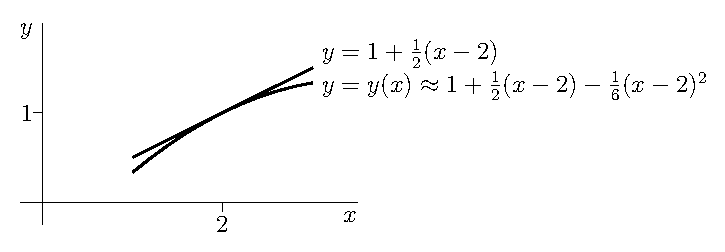
\includegraphics{graph18}
\end{center}
\end{answer}
\begin{solution}
$y$ is a function of $x$ that obeys
\begin{align*}
y(x)^4+xy(x)&=x^2-1
\intertext{
By implicit differentiation (and then subbing in $x=2$, $y(2)=1$)}
4y(x)^3y'(x)+y(x)+xy'(x)&=2x\\
 4y'(2)+1+2y'(2)&=4\\
  y'(2)&=\frac{1}{2}
\end{align*}
Differentiating with respect to $x$ a second time
and then subbing in\\ $x=2$, $y(2)=1$, $y'(2)=\frac{1}{2}$:
\begin{align*}
12y(x)^2y'(x)^2+4y(x)^3y''(x)+y'(x)+y'(x)+xy''(x)&=2\\
12\times1\times\frac{1}{4}+4y''(2)+\frac{1}{2}+\frac{1}{2}+2y''(2)&=2
\\ 6y''(2)&=-2\\
 y''(2)&=-\frac{1}{3}
\end{align*}The tangent line approximation to $y(x)$ at $x=2$ is
\begin{align*}
y(x)&\approx y(2)+y'(2)(x-2)=1+\frac{1}{2}(x-2)
\intertext{In particular,}
y(2.1)&\approx y(2)+y'(2)(2.1-2)=1+\frac{1}{2}(.1)=\boxed{1.05}
\intertext{The quadratic approximation to $y(x)$ at $x=2$ is}
y(x)&\approx y(2)+y'(2)(x-2)+\frac{1}{2} y''(2)(x-2)^2\\
&=1+\frac{1}{2}(x-2)-\frac{1}{6}(x-2)^2
\intertext{In particular, }
y(2.1)&\approx y(2)+y'(2)(2.1-2)+\frac{1}{2} y''(2)(2.1-2)^2\\
&=1+\frac{1}{2}(.1)-\frac{1}{6}(.1)^2=\boxed{1.0483}
\end{align*}
At $x=2$, $y=1$ and $y'=\frac{1}{2}$. So the tangent line passes through $(2,1)$
and has slope $\frac{1}{2}$. At $x=2$, $y''=-\frac{1}{3}$, so the graph $y=f(x)$
(locally!) looks like a parabola pointing down near $x=2$. This gives the graph fragment below.

Alternatively, we could observe that, near $x=2$, $y(x)$ will be quite close
to its quadratic approximation,
$1+\frac{1}{2}(x-2)-\frac{1}{6}(x-2)^2$.
\begin{center}
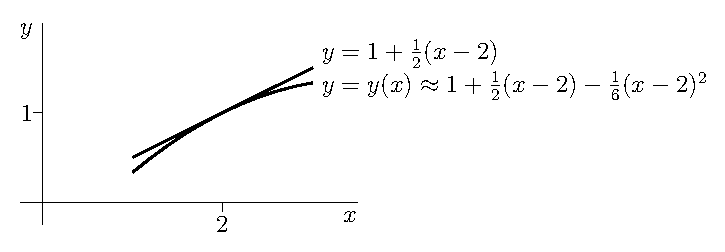
\includegraphics{graph18}
\end{center}
\end{solution}



\begin{question}[1996D]
The equation $x^4+y+xy^4=1$ defines $y$ implicitly as a function
of $x$ near the point $x=-1,~ y=1$.
\begin{enumerate}[(a)]
\item\label{s3.4tan1}  Use the tangent line approximation at the given point to
estimate the value of $y$ when $x=-0.9$.
\item\label{s3.4tan2}   Use the quadratic approximation  at the given point to get
another estimate of $y$ when $x=-0.9$.
\item\label{s3.4tan3} Make a sketch showing how
the curve relates to the tangent line at the given point.
\end{enumerate}
\end{question}
\begin{answer}
\eqref{s3.4tan1} 0.9\qquad
\eqref{s3.4tan2} {0.8867}\qquad
\eqref{s3.4tan3}
\begin{center}
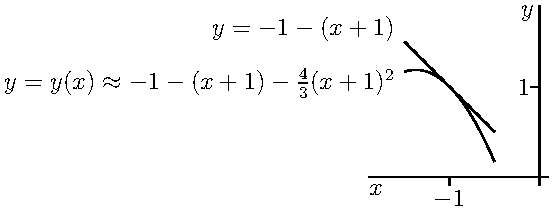
\includegraphics{graphE3b}
\end{center}\end{answer}
\begin{solution}
\eqref{s3.4tan1}
$y$ is a function of $x$ that obeys
\begin{align*}
1&=x^4+y(x)+xy(x)^4
\intertext{By implicit differentiation (and then subbing in $x=-1$, $y(-1)=1$)}
0&=4x^3+y'(x)+y(x)^4+4xy(x)^3y'(x)\\
0&= -4+y'(-1)+1-4y'(-1)\\
-1&= y'(-1)
\intertext{
Differentiating with respect to $x$ a second time
and then subbing in $x=-1$, $y(-1)=1$, and $y'(-1)=-1$:}
0&=12x^2+y''(x)+4y(x)^3y'(x)+4y(x)^3y'(x)+12xy(x)^2y'(x)^2+4xy(x)^3y''(x)\\
0&= 12+y''(-1)-4-4-12-4y''(-1)\\
-8&= 3y''(-1)\\
y''(-1)&=-\frac{8}{3}
\end{align*}
The tangent line approximation to $y(x)$ at $x=-1$ is
\begin{align*}
y(x)&\approx y(-1)+y'(-1)(x+1)=1-(x+1)=-x
\intertext{
In particular, }
y(-0.9)&\approx 0.9
\end{align*}
\eqref{s3.4tan2}
The quadratic approximation to $y(x)$ at $x=-1$ is
\begin{align*}
y(x)&\approx y(-1)+y'(-1)(x+1)+\frac{1}{2} y''(-1)(x+1)^2\\
&=1-(x+1)-\frac{4}{3}(x+1)^2
\intertext{In particular, }
y(-0.9)&\approx 1-(.1)-\frac{4}{3}(.1)^2\approx{0.8867}
\end{align*}
\eqref{s3.4tan3}
At $x=-1$, the slope of the curve is $y'(-1)=-1$. Its tangent line is falling
at $45^\circ$. At $x=-1$, $y''(-1)=-\frac{8}{3}$, so the slope of the
curve is decreasing as $x$ passes through $-1$. Zoomed in very close, the curve looks like a parabola opening downwards. This gives the figure
\begin{center}
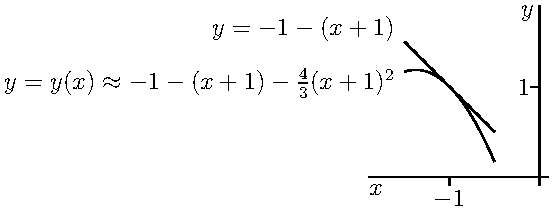
\includegraphics{graphE3b}
\end{center}\end{solution}

\begin{question}[1999H]
Given that $\log 10\approx 2.30259$, estimate $\log 10.3$ using
a suitable tangent line approximation. Give an upper and lower bound
for the error in your approximation by using a suitable error estimate.
\end{question}
\begin{answer}
$\log 10.3 \approx 2.33259$\\
The error is between
$-0.00045$ and $-0.00042$.
\end{answer}
\begin{solution}
 Let $f(x)=\log x$ and $x_0=10$. Then
\begin{align*}
f(x)&=\log x &
f'(x)&=\frac{1}{x} & f''(x)&=-\frac{1}{x^2} \\
f(10)&=\log 10\approx 2.30259 &
f'(10)&=\frac{1}{10} & f''(10)&=-\frac{1}{100}
\end{align*}
so that, with $x=10.3$,
$$
\log 10.3=f(10.3)\approx f(10)+f'(10)(10.3-10)
=2.30259+\frac{0.3}{10}
=2.33259
$$
The error in this approximation (excluding the error in the given data
$\log 10\approx 2.30259$) is $\dfrac{1}{2} f''(z)(10.3-10)^2$ for some $z$ between
$10$ and $10.3$. Because $f''(z)=-\dfrac{1}{z^2}$ increases as $z$ increases,
it must be between $-\dfrac{1}{10^2}$ and $-\dfrac{1}{10.3^2}$. This forces
$\dfrac{1}{2} f''(z)(10.3-10)^2$ to be between
$-\dfrac{1}{2}\cdot \dfrac{1}{10^2}(0.3)^2=-0.00045$ and
$-\dfrac{1}{2}\cdot \dfrac{1}{10.3^2}(0.3)^2<-0.00042$.
\end{solution}


\begin{question}[2012H]
Consider $f(x)=e^{e^x}$.
\begin{enumerate}[(a)]
\item Give the linear approximation for $f$ near $x=0$ (call this
$L(x)$).
\item Give the quadratic approximation for $f$ near $x=0$ (call
this $Q(x)$).
\item Prove that $L(x)<Q(x)<f(x)$ for all $x>0$.
\item Find an interval of length
at most $0.01$ that is guaranteed to contain the number $e^{0.1}$.
\end{enumerate}
\end{question}
\begin{hint} For (c), you can write $f(x)$ as the sum of $Q(x)$ and its error term.\\
For (d), you can use the linear approximation of $e^x$  centred at $0$, with its error term when $x=0.1$.
\end{hint}
\begin{answer}
(a) $L(x)=e+ex$ \qquad (b) $Q(x)=e+ex+ex^2$\\
(c) Since $ex^2 >0$ for all $x>0$, $L(x)<Q(x)$ for all $x>0$.

From the error formula, we know that
\begin{align*}
f(x)&=f(0)+f'(0)x+\half f''(0)x^2
+\dfrac{1}{3!}f'''(c)x^{3}\\
&=Q(x)+\frac{1}{6}\left(e^c+3e^{2c}+e^{3c}\right)e^{e^c}x^3
\end{align*}
for some $c$ between $0$ and $x$.
Since $\frac{1}{6}\left(e^c+3e^{2c}+e^{3c}\right)e^{e^c}$ is positive for any $c$, for
all $x>0$,
$\frac{1}{6}\left(e^c+3e^{2c}+e^{3c}\right)e^{e^c}x^3>0$, so
$Q(x)<f(x)$.

(d) $1.105<e^{0.1}<1.115$
\end{answer}
\begin{solution}
We begin by finding the values of the derivatives of $f$ at $x=0$. We can use the chain rule, or the formula we found in Question~\ref{s2.14expprod}, Section~\ref*{sec higher diff}.%2.14, higher order derivatives
\begin{align*}
f(x)&=e^{e^x}&f(0)&=e\\
f'(x)&=e^xe^{e^x}&f'(0)&=e\\
f''(x)&=\left(e^x+e^{2x}\right)e^{e^x}&f''(0)&=2e\\
f'''(x)&=\left(e^x+3e^{2x}+e^{3x}\right)e^{e^x}
\end{align*}

(a) $L(x)=f(0)+f'(0)(x-0)=e+ex$

(b) $Q(x)=f(0)+f'(0)(x-0)+\dfrac{1}{2}f''(0)(x-0)^2=e+ex+ex^2$

(c) Since $ex^2 >0$ for all $x>0$, $L(x)<Q(x)$ for all $x>0$.

From the error formula, we know that
\begin{align*}
f(x)&=f(0)+f'(0)x+\half f''(0)x^2
+\dfrac{1}{3!}f'''(c)x^{3}\\
&=Q(x)+\frac{1}{6}\left(e^c+3e^{2c}+e^{3c}\right)e^{e^c}x^3
\end{align*}
for some $c$ between $0$ and $x$.
Since $\frac{1}{6}\left(e^c+3e^{2c}+e^{3c}\right)e^{e^c}$ is positive for any $c$, for
all $x>0$,
$\frac{1}{6}\left(e^c+3e^{2c}+e^{3c}\right)e^{e^c}x^3>0$, so
$Q(x)<f(x)$.

(d) Write $g(x)=e^x=1+x+\dfrac{1}{2!}e^c x^2$, for some $c$ between
$0$ and $x$.
For $x=0.1$ we have $0<c<0.1$ and $1<e^c<e^{0.1}<e<3$.
So
\begin{align*}
e^{0.1}&&=&&f(0.1)&&=&&1+0.1+\half e^c (0.1)^2&&>&&1+0.1+\half (1) (0.1)^2&&=&&1.105\\
e^{0.1}&&=&&f(0.1)&&=&&1+0.1+\half e^c (0.1)^2&&<&&1+0.1+\half (3) (0.1)^2&&=&&1.115
\end{align*}
That is, $1.105<e^{0.1}<1.115$.
\end{solution}

%%%%%
\section{Optimization}
\subsection{Local and global maxima and minima}
%
% Copyright 2018 Joel Feldman, Andrew Rechnitzer and Elyse Yeager.
% This work is licensed under a Creative Commons Attribution-NonCommercial-ShareAlike 4.0 International License.
% https://creativecommons.org/licenses/by-nc-sa/4.0/
%
\questionheader{ex:s3.5.1}
%%%%%%%%%%%%%%%%%%
\subsection*{\Conceptual}
%%%%%%%%%%%%%%%%%%


\begin{Mquestion}
Identify every critical point and every singular point of $f(x)$ shown on the graph below.\\
 Which correspond to local extrema?
\begin{center}\begin{tikzpicture}
\YEaaxis{4}{4}{1}{4}
\draw[thick] plot[domain=-2.5:2](\x,{\x*\x*\x/4+2});
\draw[thick] plot[domain=2:2.5](\x,{3*(\x-3)*(\x-3)+1});
\draw[thick] plot[domain=2.5:3.1](\x,{exp(-4*(\x-2.43))+1}) node[ right]{$y=f(x)$};
\end{tikzpicture}\end{center}
\end{Mquestion}
\begin{hint}
Estimate $f'(0)$.
\end{hint}
\begin{answer}
\begin{center}\begin{tikzpicture}
\YEaaxis{4}{4}{1}{4}
\draw[thick] plot[domain=-2.5:2](\x,{\x*\x*\x/4+2});
\draw[thick] plot[domain=2:2.5](\x,{3*(\x-3)*(\x-3)+1});
\draw[thick] plot[domain=2.5:3.1](\x,{exp(-4*(\x-2.43))+1}) node[ right]{$y=f(x)$};
\draw[red] (2,4) node[vertex]{};
\draw[blue] (0,2) node[vertex]{};
\draw[thick, blue ] (0,.2)--(0,-.2);
\draw[thick, red ] (2,.2)--(2,-.2);
\end{tikzpicture}\end{center}
There is a critical point at $x=0$. The $x$-value of the red dot is a singular point, and a local maximum occurs there.
\end{answer}
\begin{solution}
\begin{center}\begin{tikzpicture}
\YEaaxis{4}{4}{1}{4}
\draw[thick] plot[domain=-2.5:2](\x,{\x*\x*\x/4+2});
\draw[thick] plot[domain=2:2.5](\x,{3*(\x-3)*(\x-3)+1});
\draw[thick] plot[domain=2.5:3.1](\x,{exp(-4*(\x-2.43))+1}) node[ right]{$y=f(x)$};
\draw[red] (2,4) node[vertex]{};
\draw[blue] (0,2) node[vertex]{};
\draw[thick, blue ] (0,.2)--(0,-.2);
\draw[thick, red ] (2,.2)--(2,-.2) node[below]{$a$};
\end{tikzpicture}\end{center}
When $x=0$, the curve $y=f(x)$ appears to have a flat tangent line, so the $x=0$ is a critical point. However, it is not a local extremum: it is not true that $f(0) \geq f(x)$ for all $x$ near 0, and it is not true that $f(0) \leq f(x)$ for all $x$ near 0.

To the right of the $x$-axis, there is a spike where the derivative of $f(x)$ does not exist. The $x$-value corresponding to this spike (call it $a$) is a singular point, and $f(x)$ has a local maximum at $x=a$.
\end{solution}


\begin{Mquestion}
Identify every critical point and every singular point of $f(x)$
on the graph below. Which correspond to local extrema? Which correspond to global extrema over the interval shown?

\begin{center}\begin{tikzpicture}[scale=0.8]
\YEaaxis{5}{5}{3}{8}
\draw[thick] plot[domain=-5:1](\x,{-(\x*1.1+5)*(\x-2)*(\x-2)/8+4});
\draw (-5,7) node[vertex]{};
\draw (1,3.25) node[opendot]{};
\draw[thick] plot[domain=1:5](\x,{-\x/4+2}) node[ above right]{$y=f(x)$};
\draw (1,1.75) node[vertex]{};
\draw (5,.75) node[vertex]{};
\end{tikzpicture}\end{center}

\end{Mquestion}
\begin{hint}
If the graph is discontinuous at a point, it is not differentiable at that point.
\end{hint}
\begin{answer}
\begin{center}\begin{tikzpicture}[scale=0.8]
\YEaaxis{5}{5}{3}{8}
\draw[thick] plot[domain=-5:1](\x,{-(\x*1.1+5)*(\x-2)*(\x-2)/8+4});
\draw (-5,7) node[vertex]{};
\draw (1,3.25) node[opendot]{};
\draw[thick] plot[domain=1:5](\x,{-\x/4+2}) node[ above right]{$y=f(x)$};
\draw (1,1.75) node[vertex]{};
\draw (5,.75) node[vertex]{};
\color{blue}
\draw (-2.36,-1.7) node[vertex]{};
\draw[thick] (-2.36,.2)--(-2.36,-.2) node[below]{$a$};
\color{red}
\draw[thick] (1,.2)--(1,-.2) node[below]{$b$};
\end{tikzpicture}\end{center}
The $x$-coordinate corresponding to the blue dot (let's call it $a$) is a critical point, and $f(x)$ has a local and global minimum at $x=a$. The $x$-coordinate corresponding to the discontinuity (let's call it $b$) is a singular point, but there is no a global or local extremum at $x=b$.
\end{answer}
\begin{solution}
\begin{center}\begin{tikzpicture}[scale=0.8]
\YEaaxis{5}{5}{3}{8}
\draw[thick] plot[domain=-5:1](\x,{-(\x*1.1+5)*(\x-2)*(\x-2)/8+4});
\draw (-5,7) node[vertex]{};
\draw (1,3.25) node[opendot]{};
\draw[thick] plot[domain=1:5](\x,{-\x/4+2}) node[ above right]{$y=f(x)$};
\draw (1,1.75) node[vertex]{};
\draw (5,.75) node[vertex]{};
\color{blue}
\draw (-2.36,-1.7) node[vertex]{};
\draw[thick] (-2.36,.2)--(-2.36,-.2) node[below]{$a$};
\color{red}
\draw[thick] (1,.2)--(1,-.2) node[below]{$b$};
\end{tikzpicture}\end{center}
The $x$-coordinate corresponding to the blue dot (let's call it $a$) is a critical point, because the tangent line to $f(x)$ at $x=a$ is horizontal. There is no lower point nearby, and actually no lower point on the whole interval shown, so $f(x)$ has both a local minimum and  a global minimum at $x=a$.

If a function is not continuous at a point, then it is not differentiable at that point. So, the $x$-coordinate  corresponding to the discontinuity (let's call it $b$) is a singular point. Values of $f(x)$ immediately to the right of $b$ are lower, and values immediately to the left of $b$ are higher, so $f(x)$ has no local (or global) extremum at $x=b$.

If we wanted to know the derivative of the function at the left endpoint, we would take the derivative from the right. This looks to be some negative real number: so it exists (therefore, the left endpoint is not a singular point) and is not zero (therefore, the left endpoint is not a critical point). Endpoints \emph{can} be critical and singular points, but this one happens to be neither.

Similarly, at the right endpoint of the interval $f'(x)$ is some negative real number, so this point is neither critical nor singular.

Remark: $f(x)$ has a global maximum at the left-most endpoint of the interval. However, we do not call this a local maximum. In order for $f(x)$ to have a local maximum at $x=c$, $c$ must be strictly inside the domain of the function. In short: \emph{endpoints can't be local extrema}.


\end{solution}


\begin{question}
Draw a graph $y=f(x)$ where a $f(2)$ is a local maximum, but it is not a  global maximum.
\end{question}
\begin{hint}
Try making a little bump at $x=2$, the letting the function get quite large somewhere else.
\end{hint}
\begin{answer}
One possible answer is shown below.
\begin{center}
\begin{tikzpicture}
\YEaaxis{1.5}{3}{3}{3}
\draw[thick] plot[domain=-1:2.5](\x,{-\x*\x*(\x-2)});
\YExcoord{1.3}{2}
\end{tikzpicture}
\end{center}
\end{answer}
\begin{solution}
One possible answer is shown below.
\begin{center}
\begin{tikzpicture}
\YEaaxis{1.5}{3}{3}{3}
\draw[thick] plot[domain=-1:2.5](\x,{-\x*\x*(\x-2)});
\YExcoord{1.3}{2}
\end{tikzpicture}
\end{center}
For every $x$ in the red interval shown below, $f(2) \geq f(x)$, so $f(2)$ is a local maximum. However, the point marked with a blue dot shows that $f(x)>f(2)$ for some $x$, so $f(2)$ is not a global maximum.
\begin{center}
\begin{tikzpicture}
\draw[dotted, fill=red!20] (1,-.5) rectangle (1.75,1.5);
\YEaaxis{1.5}{3}{3}{3}
\draw[thick] plot[domain=-1:2.4](\x,{-\x*\x*(\x-2)});
\YExcoord{1.32}{2}
\draw (-1,3) node[blue, vertex]{};
\draw[dashed,red] (1,1.2)--(1.74,1.2);
\draw (1.32,1.2) node[red, vertex]{};
\end{tikzpicture}
\end{center}
\end{solution}

%%%%%%%%%%%%%%%%%%
\subsection*{\Procedural}
%%%%%%%%%%%%%%%%%%


\begin{Mquestion}
Suppose $f(x)=\dfrac{x^2-10}{x-5}$.
\begin{enumerate}[(a)]
\item Find all critical points.
\item Find all singular points.
\item What are the possible points where local extrema of $f(x)$ may exist?
\end{enumerate}
\end{Mquestion}
\begin{hint}
Critical points are those values of $x$ in the domain of $f(x)$  for which $f'(x)=0$.
\\
Singular points are those values of $x$ in the domain of $f(x)$ for which $f(x)$ is not differentiable.
\end{hint}
\begin{answer}
The critical points are $x=5+\sqrt{15}$ and $x=5-\sqrt{15}$.
These two points are the only places where local extrema might exist.
There are no singular points.
\end{answer}
\begin{solution}
Critical points are those values of $x$ in the domain of $f(x)$  for which $f'(x)=0$, and
singular points are those values of $x$  in the domain of $f(x)$ for which $f(x)$ is not differentiable.
So, we ought to find $f'(x)$.
Using the quotient rule,
\begin{align*}
f'(x)&=\frac{(x-5)(2x)-(x^2-10)}{(x-5)^2}\\
&=\frac{x^2-10x+10}{(x-5)^2}
\intertext{The only place where this function doesn't exist is $x=5$. Since $5$ is not in the domain of $f(x)$,}
\intertext{(b) $f(x)$ has no singular points. }
\intertext{To find the critical points, we find where $f'(x)=0$. That is:}
0&=x^2-10x+10
\intertext{Using the quadratic formula,}
x&=\dfrac{10\pm\sqrt{10^2-4(1)(10)}}{2}\\
&=5 \pm \sqrt{15}
\end{align*}
(a) So the critical points of $f(x)$ are $x=5+\sqrt{15}$ and $x=5-\sqrt{15}$.

(c) Theorem~\ref*{thm:APPlocalMaxMin} tells us that local extrema of $f(x)$ can only occur at critical points and singular points.
So, the possible points where extrema of $f(x)$ may exist are $x=5+\sqrt{15}$ and $x=5-\sqrt{15}$.
\end{solution}



%%%%%%%%%%%%%%%%%%
\subsection*{\Application}
%%%%%%%%%%%%%%%%%%
\begin{Mquestion}
Below are a number of curves, all of which have a singular point at $x=2$. For each, label whether $x=2$ is a local maximum, a local minimum, or neither.
\begin{center}
\begin{tikzpicture}
\YEaaxis{.5}{2}{.5}{2};
\YExcoord{1}{2}
\draw[thick] plot[domain=-.5:1](\x,\x);
\draw[thick] plot[domain=1:2](\x,-\x+3);
\draw (1,1) node[opendot]{};
\draw (1,2) node[vertex]{};
\end{tikzpicture}
\hfill
\begin{tikzpicture}
\YEaaxis{.5}{2}{.5}{2};
\YExcoord{1}{2}
\draw[thick] plot[domain=-.5:1](\x,\x);
\draw[thick] plot[domain=1:2](\x,-\x+3);
\draw (1,2) node[opendot]{};
\draw (1,1) node[vertex]{};
\end{tikzpicture}
\hfill
\begin{tikzpicture}
\YEaaxis{.5}{2}{.5}{2};
\YExcoord{1}{2}
\draw[thick] plot[domain=-.5:1](\x,\x/2);
\draw[thick] plot[domain=1:2](\x,\x/2+1);
\draw (1,.5) node[opendot]{};
\draw (1,1.5) node[vertex]{};
\end{tikzpicture}
\hfill
\begin{tikzpicture}
\YEaaxis{.5}{2}{.5}{2};
\YExcoord{1}{2}
\draw[thick] plot[domain=-.5:1](\x,-\x/2+1);
\draw[thick] plot[domain=1:2](\x,\x/2);
\draw (1,.5) node[opendot]{};
\draw (1,1) node[vertex]{};
\end{tikzpicture}
\end{center}
\end{Mquestion}
\begin{hint}
We're only after local extrema, not global. Let $f(x)$ be our function.
If there is some interval around $x=2$ where nothing is bigger than $f(2)$, then $f(2)$ is a local maximum, whether or not it is a maximum overall.
\end{hint}
\begin{answer}
\begin{center}
\begin{tikzpicture}
\YEaaxis{.5}{2}{.5}{2};
\YExcoord{1}{2}
\draw[thick] plot[domain=-.5:1](\x,\x);
\draw[thick] plot[domain=1:2](\x,-\x+3);
\draw (1,1) node[opendot]{};
\draw (1,2) node[vertex]{};
\draw (1,-1.5) node{local max};
\end{tikzpicture}
\hfill
\begin{tikzpicture}
\YEaaxis{.5}{2}{.5}{2};
\YExcoord{1}{2}
\draw[thick] plot[domain=-.5:1](\x,\x);
\draw[thick] plot[domain=1:2](\x,-\x+3);
\draw (1,2) node[opendot]{};
\draw (1,1) node[vertex]{};
\draw (1,-1.5) node{neither};
\end{tikzpicture}
\hfill
\begin{tikzpicture}
\YEaaxis{.5}{2}{.5}{2};
\YExcoord{1}{2}
\draw[thick] plot[domain=-.5:1](\x,\x/2);
\draw[thick] plot[domain=1:2](\x,\x/2+1);
\draw (1,.5) node[opendot]{};
\draw (1,1.5) node[vertex]{};
\draw (1,-1.5) node{neither};
\end{tikzpicture}
\hfill
\begin{tikzpicture}
\YEaaxis{.5}{2}{.5}{2};
\YExcoord{1}{2}
\draw[thick] plot[domain=-.5:1](\x,-\x/2+1);
\draw[thick] plot[domain=1:2](\x,\x/2);
\draw (1,.5) node[opendot]{};
\draw (1,1) node[vertex]{};
\draw (1,-1.5) node{local max};
\end{tikzpicture}
\end{center}
\end{answer}
\begin{solution}
\begin{center}
\begin{tikzpicture}
\YEaaxis{.5}{2}{.5}{2};
\YExcoord{1}{2}
\draw[thick] plot[domain=-.5:1](\x,\x);
\draw[thick] plot[domain=1:2](\x,-\x+3);
\draw (1,1) node[opendot]{};
\draw (1,2) node[vertex]{};
\draw (1,-1.5) node{local max};
\end{tikzpicture}
\hfill
\begin{tikzpicture}
\YEaaxis{.5}{2}{.5}{2};
\YExcoord{1}{2}
\draw[thick] plot[domain=-.5:1](\x,\x);
\draw[thick] plot[domain=1:2](\x,-\x+3);
\draw (1,2) node[opendot]{};
\draw (1,1) node[vertex]{};
\draw (1,-1.5) node{neither};
\end{tikzpicture}
\hfill
\begin{tikzpicture}
\YEaaxis{.5}{2}{.5}{2};
\YExcoord{1}{2}
\draw[thick] plot[domain=-.5:1](\x,\x/2);
\draw[thick] plot[domain=1:2](\x,\x/2+1);
\draw (1,.5) node[opendot]{};
\draw (1,1.5) node[vertex]{};
\draw (1,-1.5) node{neither};
\end{tikzpicture}
\hfill
\begin{tikzpicture}
\YEaaxis{.5}{2}{.5}{2};
\YExcoord{1}{2}
\draw[thick] plot[domain=-.5:1](\x,-\x/2+1);
\draw[thick] plot[domain=1:2](\x,\x/2);
\draw (1,.5) node[opendot]{};
\draw (1,1) node[vertex]{};
\draw (1,-1.5) node{local max};
\end{tikzpicture}
\end{center}
For the first curve, the function's value at $x=2$ (that is, the $y$-value of the solid dot) is higher than anything around it. So, it's a local maximum.

For the second curve, the function's value at $x=2$ (that is, the $y$-value of the solid dot) is higher than everything to the left, but lower than values immediately to the right. (On the graph reproduced below, $f(x)$ is higher than everything in the red section, and lower than everything in the blue section.) So, it is neither a local max nor a local min.
\begin{center}
\begin{tikzpicture}
\draw[dotted, fill=red!20] (-.5,-1) rectangle (1,2.5);
\draw[dotted, fill=blue!20](1,2.5) rectangle (1.5,-1);
\YEaaxis{.5}{2}{.5}{2};
\YExcoord{1}{2}
\draw[thick] plot[domain=-.5:1](\x,\x);
\draw[thick] plot[domain=1:2](\x,-\x+3);
\draw (1,2) node[opendot]{};
\draw (1,1) node[vertex]{};
\draw[dashed] (-.5,1)--(1.5,1);
\end{tikzpicture}
\end{center}

Similarly, for the third curve, $f(2)$ is lower than the values to the right of it, and higher than values to the left of it, so it is neither a local minimum nor a local maximum.

In the final curve, $f(2)$ (remember--this is the $y$-value of the solid dot) is higher than everything immediately to the left or right of it (for instance, over the interval marked in red below), so it is a local maximum.
\begin{center}
\begin{tikzpicture}
\draw[dotted, fill=red!20] (.5,-1) rectangle (1.5,2.5);
\draw[dashed, red] (.5,1)--(1.5,1);
\YEaaxis{.5}{2}{.5}{2};
\YExcoord{1}{2}
\draw[thick] plot[domain=-.5:1](\x,-\x/2+1);
\draw[thick] plot[domain=1:2](\x,\x/2);
\draw (1,.5) node[opendot]{};
\draw (1,1) node[vertex]{};
\end{tikzpicture}
\end{center}
\end{solution}

\begin{question}
Draw a graph $y=f(x)$ where $f(2)$ is a local maximum, but $x=2$ is not a critical point.
\end{question}
\begin{hint}
By Theorem~\ref*{thm:APPlocalMaxMin},
if $x=2$ not a critical point, then it must be a singular point. Remember that \emph{endpoints} can't be local extrema.
\end{hint}
\begin{answer}
There are many possible answers. Every answer must have $x=2$ as a singular point strictly inside the domain of $f(x)$. Two possibilities are shown below.
\begin{center}
\begin{tikzpicture}
\YEaxis{2}{2}
\YExcoord{1}{2}
\draw [thick] (-2,1)--(2,1);
\draw  (1,1) node[opendot]{};
\draw (1,1.5) node[vertex]{};
\end{tikzpicture}
\hspace{2cm}
\begin{tikzpicture}
\YEaxis{2}{2}
\YExcoord{1}{2}
\draw [thick] plot[domain=-1.5:1](\x,{\x*\x/1.5+.33});
\draw [thick] plot[domain=1:2](\x,{-\x+2});
\end{tikzpicture}
\end{center}
\end{answer}
\begin{solution}
By Theorem~\ref*{thm:APPlocalMaxMin}, if $x=2$ not a critical point, then it must be a singular point. That is, $f(x)$ is not differentiable at $x=2$. Also, remember that endpoints are not local extrema. Two possibilities are shown below, but there are infinitely many possible answers.
\begin{center}
\begin{tikzpicture}
\YEaxis{2}{2}
\YExcoord{1}{2}
\draw [thick] (-2,1)--(2,1);
\draw  (1,1) node[opendot]{};
\draw (1,1.5) node[vertex]{};
\end{tikzpicture}
\hspace{2cm}
\begin{tikzpicture}
\YEaxis{2}{2}
\YExcoord{1}{2}
\draw [thick] plot[domain=-1.5:1](\x,{\x*\x/1.5+.33});
\draw [thick] plot[domain=1:2](\x,{-\x+2});
\end{tikzpicture}
\end{center}
\end{solution}




\begin{question}
 \[f(x)=\sqrt{\left|(x-5)(x+7)\right|}\]
Find all critical points and all singular points of $f(x)$. You do not have to specify whether a point is critical or singular.
\end{question}
\begin{hint}
You should be able to figure out the global minima of $f(x)$ in your head.
\\
Remember with absolute values, $|X|=\left\{\begin{array}{ll}
X&X\ge0\\
-X&X<0
\end{array}\right.$.
\end{hint}
\begin{answer}
$x=-7$, $x=-1$, and $x=5$
\end{answer}
\begin{solution}
Critical points are those values of $x$ for which $f'(x)=0$, and
singular points are those values of $x$ for which $f(x)$ is not differentiable.
So, we ought to find $f'(x)$. Since $f(x)$ has an absolute value sign, let's re-write it in a version that is friendlier to differentiation. Remember that $|X|=X$ when $X \geq 0$, and $|X|=-X$ when $X<0$.
\begin{align*}
f(x)&=\sqrt{\left|(x-5)(x+7)\right|}\\
&=\left\{\begin{array}{cc}
\sqrt{(x-5)(x+7)}&\mbox{ if } (x-5)(x+7)\ge0\\
\sqrt{-(x-5)(x+7)}&\mbox{ if } (x-5)(x+7)<0
\end{array}\right.
\intertext{The product $(x-5)(x+7)$ is positive when $(x-5)$ and $(x+7)$ have the same sign, and negative when they have opposite signs, so}
f(x)&=\left\{\begin{array}{ll}
\sqrt{(x-5)(x+7)}&\mbox{ if } x\in (-\infty,-7] \cup [5,\infty)\\
\sqrt{-(x-5)(x+7)}&\mbox{ if } x\in(-7,5)
\end{array}\right.
\intertext{Now, when $x \neq -7,5$, we can differentiate, using the chain rule.}
f'(x)&=\left\{\begin{array}{ll}
\frac{\diff{}{x}\left\{(x-5)(x+7)\right\}}{2\sqrt{(x-5)(x+7)}}&\mbox{ if } x\in (-\infty,-7) \cup (5,\infty)\\
\frac{\diff{}{x}\left\{-(x-5)(x+7)\right\}}{2\sqrt{-(x-5)(x+7)}}&\mbox{ if } x\in(-7,5)\\
?? & \mbox{ if } x=-7,\,x=5
\end{array}\right.\\
&=\left\{\begin{array}{ll}
\frac{2x+2}{2\sqrt{(x-5)(x+7)}}&\mbox{ if } x\in (-\infty,-7) \cup (5,\infty)\\
\frac{-2x-2}{2\sqrt{-(x-5)(x+7)}}&\mbox{ if } x\in(-7,5)\\
?? & \mbox{ if } x=-7,\,x=5
\end{array}\right.
\end{align*}
We are tempted to say that the derivative doesn't exist when $x=-7$ and $x=5$, but be careful-- we don't actually know that yet. The formulas we have for the $f'(x)$ are only good when $x$ is \emph{not} $-7$ or $5$.

The middle formula $\dfrac{-2x-2}{2\sqrt{-(x-5)(x+7)}}$ tells us $x=-1$ is a critical point: when $x=-1$, $f'(x)$ is given by the middle line, and it is 0. Note that $x=-1$ also makes the top formula 0, but $f'(-1)$ is not given by the top formula, so that doesn't matter.

What we've concluded so far is that $x=-1$ is a critical point of $f(x)$, and $f(x)$ has no other critical points or singular points when $x \neq -7,5$. It remains to figure out what's going on at $-7$ and $5$. One way to do this is to use the definition of the derivative to figure out what $f'(-7)$  and $f'(5)$ are, if they exist. This is somewhat laborious. Let's look for a better way.

\begin{itemize}
\item First, let's notice that $f(x)$ is defined for all values of $x$, thanks to that handy absolute value sign.
\item Next, notice $f(x) \geq 0$ for all $x$, since square roots never give a negative value.
\item Then if there is some value of $x$ that gives $f(x)=0$, that $x$ gives a global minimum, and therefore a local minimum.
\item $f(x)=0$ exactly when $(x-5)(x+7)=0$, which occurs at $x=-7$ and $x=5$
\item Therefore, $f(x)$ has global and local minima at $x=-7$ and $x=5$
\item So, $x=-7$ and $x=5$ are critical points or singular points by Theorem~\ref*{thm:APPlocalMaxMin}.
\end{itemize}

So, all together:

$x=-1$ is a critical point, and $x=-7$ and $x=5$ are critical points or singular pints (but we don't know which).

Remark: if you would like a review of how to use the definition of the derivative, below we show that $f(x)$ is not differentiable at $x=-7$. (In fact, $x=-7$ and $x=5$ are both singular points.)

\begin{align*}
f'(-7)&=\lim_{h \to 0} \frac{f(-7+h)-f(-7)}{h}\\
&=\lim_{h \to 0} \frac{\sqrt{|(-13+h)(h)|}-\sqrt{|0|}}{h}\\
&=\lim_{h \to 0} \frac{\sqrt{|(-13+h)(h)|}}{h}
\intertext{Let's first consider the case $h>0$.}
\lim_{h \to 0^+} \frac{\sqrt{|(-13+h)(h)|}}{h}&=\lim_{h \to 0^+}\frac{\sqrt{(13-h)(h)}}{h}\\
&=\lim_{h \to 0^+}\frac{\sqrt{13h-h^2}}{\sqrt{h^2}}\\
&=\lim_{h \to 0^+}\sqrt{\frac{13h-h^2}{h^2}}\\
&=\lim_{h \to 0^+}\sqrt{\frac{13}{h}-1}\\
&=\infty
\intertext{Since one side of the limit doesn't exist,}
\lim_{h \to 0} \frac{f(-7+h)-(-7)}{h}&=DNE
\intertext{so $f'(x)$ is not differentiable at $x=-7$. Therefore, $x=-7$ is a singular point.}
\end{align*}
\end{solution}


\begin{question}
Suppose $f(x)$ is the constant function $f(x)=4$. What are the critical points and singular points of $f(x)$? What are its local and global maxima and minima?
\end{question}
\begin{hint}
Review the definitions of critical points and extrema: Definition~\ref*{def:APPcriticalPoint}
and
Definition~\ref*{def:APPlocalMaxMin}.
\end{hint}
\begin{answer}
Every real number $c$ is a critical point of $f(x)$, and $f(x)$ has a local and global maximum and minimum at $x=c$. There are no singular points.
\end{answer}
\begin{solution}
For any real number $c$, $c$ is in the domain of $f(x)$ and $f'(c)$ exists and is equal to zero. So, following
Definition~\ref*{def:APPcriticalPoint}, every real number is  a critical point of $f(x)$, and $f(x)$ has no singular points.

For every number $c$, let $a=c-1$ and $b=c+1$, so $a<c<b$. Then $f(x)$ is defined for every $x$ in the interval $[a,b]$, and
$f(x) =f(c)$ for every $a \le x \le b$. That means $f(x) \leq f(c)$ and $f(x) \geq f(c)$. So, comparing with Definition~\ref*{def:APPlocalMaxMin}, we see that $f(x)$ has a global and local maximum AND minimum at every real number $x=c$.
\end{solution}

\subsection{Finding global maxima and minima}
%
% Copyright 2018 Joel Feldman, Andrew Rechnitzer and Elyse Yeager.
% This work is licensed under a Creative Commons Attribution-NonCommercial-ShareAlike 4.0 International License.
% https://creativecommons.org/licenses/by-nc-sa/4.0/
%
\questionheader{ex:s3.5.2}
%%%%%%%%%%%%%%%%%%
\subsection*{\Conceptual}
%%%%%%%%%%%%%%%%%%



\begin{question}
Sketch a function $f(x)$ such that:
\begin{itemize}
\item $f(x)$ is defined over all real numbers
\item $f(x)$ has a global max but no global min.
\end{itemize}
\end{question}
\begin{hint}
One way to avoid a global minimum is to have $\ds\lim_{x \to \infty}f(x)=-\infty$. Since $f(x)$ keeps getting lower and lower, there is no one value that is the lowest.
\end{hint}
\begin{answer}
Two examples are given below, but many are possible.
\begin{center}
\begin{tikzpicture}
\YEaaxis{2}{2}{4}{1}
\draw plot[domain=-1.75:1.75](\x,{-\x*\x}) node[right]{$y=f(x)$};
\end{tikzpicture}
\hspace{2cm}
\begin{tikzpicture}
\YEaaxis{3}{3}{1}{2}
\draw plot[domain=-2.75:-.1, samples=100](\x,{-sqrt(abs(\x))}) ;
\draw plot[domain=.1:2.75, samples=100](\x,{-sqrt(abs(\x))}) node[right]{$y=f(x)$};
\draw plot[domain=-.1:.1, samples=100](\x,{-sqrt(abs(\x))}) ;
\end{tikzpicture}
\end{center}
\end{answer}
\begin{solution}
Two examples are given below, but many are possible.
\begin{center}
\begin{tikzpicture}
\YEaaxis{2}{2}{4}{1}
\draw plot[domain=-1.75:1.75](\x,{-\x*\x}) node[right]{$y=-x^2$};
\end{tikzpicture}
\hspace{2cm}
\begin{tikzpicture}
\YEaaxis{3}{3}{1}{2}
\draw plot[domain=-2.75:-.1, samples=100](\x,{-sqrt(abs(\x))}) ;
\draw plot[domain=.1:2.75, samples=100](\x,{-sqrt(abs(\x))}) node[right]{$y=-\sqrt{|x|}$};
\draw plot[domain=-.1:.1, samples=100](\x,{-sqrt(abs(\x))}) ;
\end{tikzpicture}
\end{center}
If $f(x)=-x^2$ or $f(x)=-\sqrt{|x|}$, then $f(x)$ has a global maximum at $x=0$. Since $f(x)$ keeps getting more and more strongly negative as $x$ gets farther and farther from 0, $f(x)$ has no global minimum.
\end{solution}


\begin{Mquestion}
Sketch a function $f(x)$ such that:
\begin{itemize}
\item $f(x)$ is defined over all real numbers
\item $f(x)$ is always positive
\item $f(x)$ has no global max and no global min.
\end{itemize}
\end{Mquestion}
\begin{hint}
Try allowing the function to approach the $x$-axis without ever touching it.
\end{hint}
\begin{answer}
Two examples are given below, but many are possible.
\begin{center}
\begin{tikzpicture}
\YEaaxis{2}{2}{1}{4}
\draw plot[domain=-1.75:2](\x,{exp(\x)/2}) node[right]{$y=e^x$};
\end{tikzpicture}

\begin{tikzpicture}
\YEaaxis{6}{6}{1}{4}
\draw plot[domain=-1.4:1.4]({tan(\x r)},\x+2) node[right]{$y=\arctan x+2$};
\end{tikzpicture}
\end{center}
\end{answer}
\begin{solution}
Two examples are given below, but many are possible.
\begin{center}
\begin{tikzpicture}
\YEaaxis{2}{2}{1}{4}
\draw plot[domain=-1.75:2](\x,{exp(\x)/2}) node[right]{$y=e^x$};
\end{tikzpicture}
\end{center}
If $f(x)=e^x$, then $f(x) > 0$ for all $x$. As we move left along the $x$-axis, $f(x)$ gets smaller and smaller, approaching 0 but never reaching it. Since $f(x)$ gets smaller and smaller as we move left, there is no global minimum. Likewise, $f(x)$ increases more and more as we move right, so there is no maximum.
\begin{center}
\begin{tikzpicture}
\YEaaxis{6}{6}{1}{4}
\draw plot[domain=-1.4:1.4]({tan(\x r)},\x+2) node[right]{$y=\arctan x+2$};
\end{tikzpicture}
\end{center}
If $f(x)=\arctan(x)+2$, then $f(x) >\left(-\frac{\pi}{2}\right)+2>0$ for all $x$.

As we move left along the $x$-axis, $f(x)$ gets smaller and smaller, approaching $\left(-\frac{\pi}{2}+2\right)$ but never reaching it. Since $f(x)$ gets smaller and smaller as we move left, there is no global minimum.

 Likewise, as we move right along the $x$-axis,
$f(x)$ gets bigger and bigger, approaching $\left(\frac{\pi}{2}+2\right)$ but never reaching it. Since $f(x)$ gets bigger and bigger as we move right, there is no global maximum.
\end{solution}


\begin{question}
Sketch a function $f(x)$ such that:
\begin{itemize}
\item $f(x)$ is defined over all real numbers
\item $f(x)$ has a global minimum at $x=5$
\item $f(x)$ has a global minimum at $x=-5$, too.
\end{itemize}
\end{question}
\begin{hint}
Since the global minimum value occurs at $x=5$ and $x=-5$, it must be true that $f(5)=f(-5)$.
\end{hint}
\begin{answer}
One possible answer:
\begin{center}
\begin{tikzpicture}
\YEaaxis{4}{4}{2}{5}
\draw plot[domain=-3.5:3.5, samples=100](\x,{(\x*\x-9)*(\x*\x+9)*\x*\x/200}) node[right]{$y=f(x)$};
\YExcoord{-2.3}{-5}
\YExcoord{2.3}{5}
\end{tikzpicture}
\end{center}
\end{answer}
\begin{solution}
Since $f(5)$ is a global minimum, $f(5) \leq f(x)$ for all $x$, and so in particular $f(5) \leq f(-5)$.\\
Similarly, $f(-5) \leq f(x)$ for all $x$, so in particular $f(-5) \leq f(5)$. \\
Since $f(-5) \leq f(5)$ AND $f(5) \leq f(-5)$, it must be true that $f(-5)=f(5)$.

A sketch of one such graph is below.
\begin{center}
\begin{tikzpicture}
\YEaaxis{4}{4}{2}{5}
\draw plot[domain=-3.5:3.5, samples=100](\x,{(\x*\x-9)*(\x*\x+9)*\x*\x/200}) node[right]{$y=f(x)$};
\YExcoord{-2.3}{-5}
\YExcoord{2.3}{5}
\end{tikzpicture}
\end{center}

\end{solution}


%%%%%%%%%%%%%%%%%%
\subsection*{\Procedural}
%%%%%%%%%%%%%%%%%%


\begin{question}
$f(x)=x^2+6x-10$.
Find all global extrema on the interval $[-5,5]$
\end{question}
\begin{hint}
Global extrema will either occur at critical points in the interval $(-5,5)$ or at the endpoints $x=5,\,x=-5$.
\end{hint}
\begin{answer}
The global maximum is 45 at $x=5$ and the global minimum is $-19$ at $x=-3$.
\end{answer}
\begin{solution}
Global extrema will occur at critical or singular points in the interval $(-5,5)$ or at the endpoints $x=5,\,x=-5$.

$f'(x)=2x+6$. Since this is defined for all real numbers, there are no singular points. The only time $f'(x)=0$ is when $x=-3$. This is inside the interval $[-5,5]$. So, our points to check are $x=-3,\,x=-5,$ and $x=5$.

\begin{center}
\begin{tabular}{|c||c|c|c|}
\hline
$c$ & $-3$ &  $-5$ &  $5$ \\
\hline
type & critical point & endpoint & endpoint  \\
\hline
$f(c)$ & $-19$ & $-15$ & $45$\\
\hline
\end{tabular}
\end{center}
The global maximum is 45 at $x=5$ and the global minimum is $-19$ at $x=-3$.
\end{solution}


\begin{Mquestion}
$f(x)=\dfrac{2}{3}x^3-2x^2-30x+7$.
Find all global extrema on the interval $[-4,0]$.
\end{Mquestion}
\begin{hint}
You only need to consider critical points that are in the interval $(-4,0).$
\end{hint}
\begin{answer}
The global maximum over the interval is $61$ at $x=-3$, and the global minimum is $7$ at $x=0$.
\end{answer}
\begin{solution}
Global extrema will occur at the endpoints of the interval, $x=-4$ and $x=0$, or at singular or critical points inside the interval. Since $f(x)$ is a polynomial, it is differentiable everywhere, so there are no singular points. To find the critical points, we set the derivative equal to zero.
\begin{align*}
f'(x)&=2x^2-4x-30\\
0&=2x^2-4x-30
&=(2x-10)(x+3)\\
x&=5,\,-3
\end{align*}
The only critical point inside the interval is $x=-3$.


\begin{center}
\begin{tabular}{|c||c|c|c|}
\hline
$c$ & $-3$ &  $-4$ &  $0$ \\
\hline
type & critical point & endpoint & endpoint  \\
\hline
$f(c)$ & $61$ & $\frac{157}{3}=52+\frac{1}{3}$ & $7$\\
\hline
\end{tabular}
\end{center}
The global maximum over the interval is $61$ at $x=-3$, and the global minimum is $7$ at $x=0$.
\end{solution}

\subsection{Max/min examples}
%
% Copyright 2018 Joel Feldman, Andrew Rechnitzer and Elyse Yeager.
% This work is licensed under a Creative Commons Attribution-NonCommercial-ShareAlike 4.0 International License.
% https://creativecommons.org/licenses/by-nc-sa/4.0/
%
\questionheader{ex:s3.5.3}
%%%%%%%%%%%%%%%%%%
\subsection*{\Procedural}
%%%%%%%%%%%%%%%%%%
\Instructions{For Questions~
\ref{s3.5.3given1} through
\ref{s3.5.3given3}, the quantity to optimize is already given to you as a function of a single variable.}

\begin{question}[2015Q]\label{s3.5.3given1}
Find the global maximum and the global minimum for $f(x)=x^5 - 5x + 2$ on the interval $[-2,0]$.
\end{question}
\begin{hint}
Factor the derivative.
\end{hint}
\begin{answer}
The global maximum is $f(-1) = 6$, the global minimum is $f(-2) = -20$.
\end{answer}
\begin{solution}
We compute $f'(x)=5\,x^4 - 5$, which means that $f(x)$ has no singular points (i.e., it is
differentiable for all values of $x$), but it has two critical points:
\begin{align*}
0&=5x^4-5\\
0&=x^4-1=(x^2+1)(x^2-1)\\
0&=x^2-1\\
x&= \pm 1
\end{align*}
Note, however, that $1$ is not in the interval $[-2,0]$.

The global maximum and the
global minimum for $f(x)$ on the interval $[-2,0]$ will occur at $x=-2$, $x=0$, or $x=-1$.
\begin{center}
\begin{tabular}{|c||c|c|c|}
\hline
$c$ & $-2$ &  $0$ &  $-1$  \\
\hline
type & endpoint & endpoint & critical point  \\
\hline
$f(c)$ & $-20$ & $2$ & $6$ \\
\hline
\end{tabular}
\end{center}

So, the global maximum is $f(-1) = 6$ while the global minimum is $f(-2) = -20$.
\end{solution}



\begin{question}[2015Q]
Find the global maximum and the global minimum for $f(x)=x^5 - 5x - 10$ on the interval $[0,2]$.
\end{question}
\begin{hint} Remember to test endpoints.
\end{hint}
\begin{answer} Global maximum is $f(2) = 12$, global minimum is $f(1) = -14$.
\end{answer}
\begin{solution} We compute $f'(x)=5x^4-5$, which means that $f(x)$ has no singular points (i.e., it is differentiable for all values of $x$), but it has two critical points:
\begin{align*}
0&=5x^4-5\\
0&=x^4-1=(x^2+1)(x^2-1)\\
0&=x^2-1\\
x&= \pm 1
\end{align*}
Note, however, that $-1$ is not in the interval $[0,2]$.

The global maximum and the
global minimum for $f(x)$ on the interval $[0,2]$ will occur at $x=2$, $x=0$, or $x=1$.
\begin{center}
\begin{tabular}{|c||c|c|c|}
\hline
$c$ & $2$ &  $0$ &  $1$  \\
\hline
type & endpoint & endpoint & critical point  \\
\hline
$f(c)$ & $12$ & $-10$ & $-14$ \\
\hline
\end{tabular}
\end{center}

So, the global maximum is $f(2) = 12$ while the global minimum is $f(1) = -14$.
\end{solution}


\begin{question}[2015Q]\label{s3.5.3given3}
Find the global maximum and the global minimum for $f(x)=2x^3 - 6x^2 - 2$ on the interval $[1,4]$.
\end{question}
\begin{answer}
Global maximum is $f(4) = 30$, global minimum is $f(2) = -10$.
\end{answer}
\begin{solution}
We compute $f'(x)=6x^2 - 12x = 6x(x-2)$, which means that $f(x)$ has no singular points
(i.e., it is differentiable for all values of $x$), but it has the two critical points:
$x=0$ and $x=2$.
Note, however, $0$ is not in the interval $[1,4]$.
\begin{center}
\begin{tabular}{|c||c|c|c|}
\hline
$c$ & $1$ &  $4$ &  $2$  \\
\hline
type & endpoint & endpoint & critical point  \\
\hline
$f(c)$ & $-6$ & $30$ & $-10$ \\
\hline
\end{tabular}
\end{center}

So, the global maximum is $f(4) = 30$ while the global minimum is $f(2) = -10$.
\end{solution}


\Instructions{For Questions~\ref{s3.5.3firstderivfirst} and \ref{s3.5.3firstderivlast}, you  can decide whether a critical point is a local extrema by considering the derivative of the function.}

\begin{Mquestion}[2015Q]\label{s3.5.3firstderivfirst}
Consider the function $h(x)=x^3-12x+4$.
What are the coordinates of the local maximum of $h(x)$? What are the coordinates of the local minimum of $h(x)$?
\end{Mquestion}
\begin{hint}
One way to decide whether a critical point $x=c$ is a local extremum is to consider the first derivative. For example: if $f'(x)$ is negative for all $x$ just to the left of $c$, and positive for all $x$ just to the right of $c$, then $f(x)$ decreases up till $c$, then increases after $c$, so $f(x)$ has a local minimum at $c$.
\end{hint}
\begin{answer} Local max at $(-2,20)$, local min at $(2,-12)$.
\end{answer}
\begin{solution}
Since $h(x)$ is a polynomial, it has no singular points. We compute its critical points:
\begin{align*}
h'(x)&=3x^2-12\\
0&=3x^2-12\\
x&=\pm 2
\end{align*}
Notice as $x\to\infty$, $h(x)\to\infty$, and as $x\to-\infty$ $h(x)\to-\infty$. So Theorem~\ref*{thm:maxMinOnR} doesn't exactly apply. Instead, let's consider the signs of $h'(x)$.

\begin{center}
\begin{tabular}{|c||c|c|c|}
\hline
$x$ & $(-\infty,-2)$ &  $(-2,2)$ &  $(2,\infty)$  \\
\hline
$h'(x)$ & $>0$ & $<0$ & $>0$ \\
\hline
$h(x)$ & increasing & decreasing & increasing  \\
\hline
\end{tabular}
\end{center}
So, $h(x)$ increases until $x=-2$, then decreases. That means $h(x)$ has a local maximum at $x=-2$. The function decreases from $-2$ until $2$, after which is increases, so $h(x)$ has a local minimum at $x=2$.
We compute $f(-2)=20$ and $f(2)=-12$.
\end{solution}



\begin{question}[2015Q]\label{s3.5.3firstderivlast}
Consider the function $h(x)=2x^3-24x+1$.
What are the coordinates of the local maximum of $h(x)$? What are the coordinates of the local minimum of $h(x)$?
\end{question}
\begin{hint}
One way to decide whether a critical point $x=c$ is a local extremum is to consider the first derivative. For example: if $f'(x)$ is negative for all $x$ just to the left of $c$, and positive for all $x$ just to the right of $c$, then $f(x)$ decreases up till $c$, then increases after $c$, so $f(x)$ has a local minimum at $c$.
\end{hint}
\begin{answer}
$(-2,33)$ max, and $(2,-31)$ min
\end{answer}
\begin{solution}
Since $h(x)$ is a polynomial, it has no singular points. We compute its critical points:
\begin{align*}
h'(x)&=6x^2-24\\
0&=6x^2-24\\
x&=\pm2
\end{align*}
Notice as $x\to\infty$, $h(x)\to\infty$, and as $x\to-\infty$ $h(x)\to-\infty$. So Theorem~\ref*{thm:maxMinOnR} doesn't exactly apply. Instead, let's consider the signs of $h'(x)$.

\begin{center}
\begin{tabular}{|c||c|c|c|}
\hline
$x$ & $(-\infty,-2)$ &  $(-2,2)$ &  $(2,\infty)$  \\
\hline
$h'(x)$ & $>0$ & $<0$ & $>0$ \\
\hline
$h(x)$ & increasing & decreasing & increasing  \\
\hline
\end{tabular}
\end{center}
So, $h(x)$ increases until $x=-2$, then decreases. That means $h(x)$ has a local maximum at $x=-2$. The function decreases from $-2$ until $2$, after which is increases, so $h(x)$ has a local minimum at $x=2$.

 We compute $f(-2)=33$ and $f(2)=-31$.
\end{solution}


\Instructions{For Questions \ref{s3.5.3formulafirst} through \ref{s3.5.3formulalast}, you will have to find an expression for the quantity you want to optimize as a function of a single variable.}





\begin{Mquestion}[1999H, 2012H]\label{s3.5.3formulafirst}
You are in a dune buggy at a point $P$ in the desert, 12
km due south of the nearest point $A$ on a straight east-west road. You
want to get to a town $B$ on the road $18$ km east of $A$. If your dune
buggy can travel at an average speed of 15 km/hr through the desert and
30 km/hr along the road, towards what point $Q$ on the road should you
head to minimize your travel time from $P$ to $B$?

%\centerline{\figput{dune}}
\begin{center}
\begin{tikzpicture}
\draw[gray, line width=5pt, opacity=0.5] (-.5,3) -- (4.5,3);
\draw (0,3) node[vertex, label=above:$A$](A){};
\draw (3,3) node[vertex, label=above:$Q$](Q){};
\draw (4,3) node[vertex, label=above:$B$](B){};
\draw (0,0) node[vertex, label=left:$P$](P){};
\draw (A)--(P) node[midway, left]{12 km};
\draw[very thick] (P)--(Q)--(B);
\end{tikzpicture}
\end{center}
\end{Mquestion}
\begin{hint} Start with a formula for travel time from $P$ to $B$. You might want to assign a variable to the distance from $A$ where your buggy first reaches the road.
\end{hint}
\begin{answer} $Q$ should be $4\sqrt{3}$ kilometres from $A$
\end{answer}
\begin{solution}
Suppose that $Q$ is a distance of $x$ from $A$.
Then it is a distance of $18-x$ from $B$.
\begin{center}
\begin{tikzpicture}
\draw[gray, line width=5pt, opacity=0.5] (-.5,3) -- (4.5,3);
\draw (0,3) node[vertex, label=above:$A$](A){};
\draw (3,3) node[vertex, label=above:$Q$](Q){};
\draw (4,3) node[vertex, label=above:$B$](B){};
\draw (0,0) node[vertex, label=left:$P$](P){};
\draw (A)--(P) node[midway, left]{12 km};
\draw[very thick] (P)--(Q)--(B);
\draw[decorate, decoration={brace, amplitude=7pt}](0,3.75)--(3,3.75) node[midway, yshift=.5cm]{$x$};
\draw[decorate, decoration={brace, amplitude=7pt}](3,3.75)--(4,3.75) node[midway, yshift=.5cm]{$18-x$};
\end{tikzpicture}
\end{center}
Using the Pythagorean Theorem, the distance from $P$ to $Q$ is $\sqrt{12^2+x^2}$ kilometres, and the buggy travels 15 kph over this off-road stretch.
The travel time
from $P$ to $Q$ is $\dfrac{\sqrt{12^2+x^2}}{15}$ hours.

The distance from $Q$ to $B$ is $18-x$ kilometres, and the dune buggy travels $30$ kph along this road. The travel time from $Q$
to $B$ is $\dfrac{18-x}{30}$ hours.
So, the total travel time is
\[f(x)= \dfrac{\sqrt{12^2+x^2}}{15}+\dfrac{18-x}{30}.\] We wish to minimize
this for $0\le x\le 18$. We will test all singular points, critical points, and endpoints to find which yields the smallest value of $f(x)$. Since there are no singular points, we begin by locating the critical points.
\begin{align*}
0=f'(x)&=\dfrac{1}{15}\cdot\dfrac{1}{2}(144+x^2)^{-1/2}(2x)-\dfrac{1}{30}\\
\dfrac{1}{15}\cdot\dfrac{x}{\sqrt{144+x^2}}&=\dfrac{1}{30}\\
 \dfrac{x}{\sqrt{144+x^2}}&=\dfrac{1}{2}\\
 \dfrac{x^2}{144+x^2}&=\dfrac{1}{4}\\
 4x^2&=144+x^2\\
 x&=\dfrac{12}{\sqrt{3}}=4\sqrt{3}
\end{align*}
So the minimum travel times must be one of $f(0)$, $f(18)$, and $f\left(4\sqrt{3}\right)$.
\begin{align*}
f(0)&=\dfrac{12}{15}+\dfrac{18}{30}=1.4\cr
f(18)&=\dfrac{\sqrt{12^2+18^2}}{15}\approx1.44\cr
f\left({4\sqrt{3}}\right)&=
\dfrac{\sqrt{144+144/3}}{15}+\dfrac{18-12/\sqrt{3}}{30}
\approx1.29
\end{align*}
So $Q$ should be $4\sqrt{3}$ km from $A$.
\end{solution}

\begin{question}[1997D]
A closed three dimensional box is to be constructed in such
a way that its volume is 4500 cm${}^3$. It is also specified that the length
of the base is 3 times the width of the base. Find the dimensions of the
box that satisfies these conditions and has the minimum possible
surface area. Justify your answer.
\end{question}
\begin{hint}
A box has three dimensions; make variables for them, and write the relations given in the problem in terms of these variables.
\end{hint}
\begin{answer}
$10\times 30 \times 15$
\end{answer}
\begin{solution}
Let $\ell,\ w$ and $h$ denote the length, width and height
of the box respectively.
 We are told that $\ell w h =4500$ and that
$\ell=3w$. Hence $h=\dfrac{4500}{\ell w}=\dfrac{4500}{3 w^2}=\dfrac{1500}{w^2}$.
The surface area of the box is
$$
A=2\ell w+2\ell h+2 wh=2\left(3w^2+3w\dfrac{1500}{w^2}+w\dfrac{1500}{w^2}\right)
=2\left(3w^2+\dfrac{6000}{w}\right)=6\left(w^2+\dfrac{2000}{w}\right)
$$
\begin{center}
\begin{tikzpicture}
\draw (0,0) rectangle (2,3);
\draw[fill=gray!15] (2,3)--(4,4)--(4,1)--(2,0)--cycle;
\draw[fill=gray!5] (0,3)--(2,4)--(4,4)--(2,3)--cycle;
\draw (1,0) node[below]{$w$};
\draw (0,1.5) node[left]{$h$};
\draw (3,.5) node[below]{$\ell$};
\draw (1,1.5) node{$wh$};
\draw (2,3.5) node[rotate=-10]{$\ell w$};
\draw (3,2) node[rotate=10]{$\ell h$};
\end{tikzpicture}
\end{center}
As $w$ tends to zero or to infinity, the surface area approaches infinity.
By Theorem~\ref*{thm:maxMinOnR} the minimum surface area must occur at a critical point of
$w^2+\dfrac{2000}{w}$.
\begin{align*}
0&=\diff{}{w}\left\{w^2+\dfrac{2000}{w}\right\}\\
&=2w-\dfrac{2000}{w^2}\\
2w&=\dfrac{2000}{w^2}\\
w^3&=1000\hskip-3pt\\
 w&=10
 \intertext{Therefore,}
  \ell&=3w=30\\
   h&=\frac{1500}{w^2}=15.
\end{align*}
The dimensions of the box with minimum surface area are $10 \times 30 \times 15$.
\end{solution}






\begin{Mquestion}[1996D]
A closed rectangular container with a square base is to be made
from two different materials. The material for the base costs \$5 per square
metre, while the material for the other five sides costs \$1 per square
metre. Find the dimensions of the container which has the largest possible
volume if the total cost of materials is \$72.
\end{Mquestion}
\begin{hint} Find a formula for the cost of the base, and another formula for the cost of the other sides. The total cost is the sum of these two formulas.
\end{hint}
\begin{answer}
$2\times 2\times 6$
\end{answer}
\begin{solution}
Let the length of the sides of the square base be $b$ metres
and let the height be $h$ metres. The area of the base is $b^2$, the area
of the top is $b^2$  and the
area of each of the remaining four sides is $bh$ so the total cost is
\[
\underbrace{5(b^2)}_{\mbox{cost of base}}+\underbrace{1(b^2+4bh)}_{\mbox{cost of 5 sides}}=6b^2+4bh=72\]
{Solving for $h$,}
\begin{align*}
h&=\dfrac{72-6b^2}{4b}\\
&=\dfrac{6}{4}\left(\dfrac{12-b^2}{b}\right)\\
&=\dfrac{3}{2}\left(\dfrac{12-b^2}{b}\right)
\end{align*}
The volume is
\begin{align*}
V=b^2h&=b^2\cdot \dfrac{3}{2}\left(\dfrac{12-b^2}{b}\right)
\\
&=18b-\dfrac{3}{2}b^3.
\end{align*}
This is the function we want to maximize.
Since volume is never negative, the endpoints of the functions are the values of $b$ that make the volume 0. So, the maximum volume will not occur at an endpoint, it will occur at a critical point.
The only critical point is $b=2$:
\begin{align*}
0&=\diff{}{b}\left\{18b-\dfrac{3}{2}b^3\right\}\\
&=18-\dfrac{9}{2}b^2\\
 b^2&=4\\
  b&=2,\ h=\dfrac{3}{2}\left(\dfrac{12-4}{2}\right)=6
\end{align*}
The desired dimensions are $2\times 2\times 6$.
\end{solution}



\begin{question}[1998H]
Find a point $X$ on the positive $x$--axis and a point $Y$
on the positive $y$--axis such that (taking $O=(0,0)$)
\begin{enumerate}[(i)]
\item\label{s3.5inscribed1}The triangle $XOY$ contains the first quadrant portion of
the unit circle $x^2+y^2=1$ and
\item\label{s3.5inscribed2} the area of the triangle $XOY$ is as small as possible.
\end{enumerate}
A complete and careful mathematical justification of property \eqref{s3.5inscribed1}
is required.
\end{question}
\begin{hint}
The setup is this:
\begin{center}
\begin{tikzpicture}
\YEaxis{3}{3}
\YExcoord{2.5}{X}
\YEycoord{2}{Y}
\draw (0,0) node[below left]{$O$};
\draw[fill=gray!10] (0,0)--(2.5,0)--(0,2)--cycle;
\draw (1,0) arc (0:90:1cm);
\draw[dashed] (0,1) arc(90:360:1cm);
\end{tikzpicture}
\end{center}
\end{hint}
\begin{answer}
$X=Y=\sqrt{2}$
\end{answer}
\begin{solution}
 It suffices to consider $X$ and $Y$ such that the line $XY$
is tangent to the circle. Otherwise we could reduce the area of the triangle
by, for example, holding $X$ fixed and reducing $Y$. So let $X$ and $Y$
be the $x$-- and $y$--intercepts of the line tangent to the circle at
$(\cos\theta,\sin\theta)$. Then $\dfrac{1}{X}=\cos\theta$ and
$\dfrac{1}{Y}=\cos\left(\dfrac{\pi}{2}-\theta\right)
=\sin\theta$. The area of the triangle is
$$
\dfrac{1}{2} XY=\dfrac{1}{2\cos\theta\sin\theta}=\dfrac{1}{\sin(2\theta)}
$$

 \begin{center}
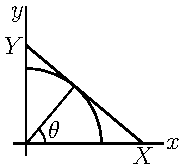
\includegraphics{minTriangle}
\end{center}

%\lower1.0in\vtop{\hsize=2.5truein \figput{minTriangle}}

This is a minimum when $\sin(2\theta)$ is a maximum. That is when
$2\theta=\dfrac{\pi}{2}$. Hence $X=\dfrac{1}{\cos(\pi/4)}$ and
$Y=\dfrac{1}{\sin(\pi/4)}$. That is, $X=Y=\sqrt{2}$.

\end{solution}



\begin{Mquestion}[2006H]
 A rectangle is inscribed in a semicircle of radius $R$
so that one side of the rectangle lies along a diameter of the semicircle.
Find the largest possible perimeter of such a rectangle, if it exists,
or explain why it does not. Do the same for the smallest possible perimeter.
\begin{center}\begin{tikzpicture}
\draw[thick] (3,0) arc (0:180:3cm) --cycle;
\draw (2,0)--(2,2.24)-|(-2,0);
\end{tikzpicture}\end{center}
\end{Mquestion}
\begin{hint}
Put the whole system on $xy$-axes, so that you can easily describe the pieces using $(x,y)$-coordinates.
\end{hint}
\begin{answer}
The largest possible perimeter is $2\sqrt{5}R$ and
the smallest possible perimeter is $2R$.
\end{answer}
\begin{solution}
For ease of notation, we place the semicircle on a Cartesian plane with diameter along the $x$-axis and centre at the origin.
\begin{center}\begin{tikzpicture}
\YEaaxis{4}{4}{.5}{4}
\draw[thick] (3,0) arc (0:180:3cm) --cycle;
\draw (2,0)--(2,2.24)-|(-2,0);
\draw (2,.2)--(2,-.2) node[below]{$x$};
\draw[dashed] (0,0)--(2,2.24) node[midway, left]{$R$};
\end{tikzpicture}\end{center}
If $x$ is the point where the rectangle touches the diameter to the right of the $y$-axis, then $2x$ is the width of the rectangle. The origin and the two right corners of the rectangle form a right triangle with hypotenuse $R$, so by the Pythagorean Theorem,
the upper right hand corner
of the rectangle is at $\big(x,\sqrt{R^2-x^2}\big)$. The perimeter of the rectangle is given by the function:
\begin{align*}
P(x)&=4x+2\sqrt{R^2-x^2}
\intertext{So, this is what we optimize. The endpoints of the domain for this function are $x=0$ and $x=R$. To find the critical points, we differentiate:}
 P'(x)&=4-\dfrac{2x}{\sqrt{R^2-x^2}}\\
P'(x)=0\iff 4&=\dfrac{2x}{\sqrt{R^2-x^2}}\\
 x&=2\sqrt{R^2-x^2}\\
x^2&=4(R^2-x^2)\\
5x^2&=4R^2\\
x&=\dfrac{2}{\sqrt{5}}R
\end{align*}
Note that since our perimeter formula was defined to work only for $x$ in $[0,R]$, we neglect the negative square root, $-\dfrac{2}{\sqrt{5}}R$.

Now, we find the size of the perimeter at the critical point and the endpoints:

\begin{center}
\begin{tabular}{|c||c|c|c|}
\hline
$c$ & $0$ &  $R$ &  $\frac{2}{\sqrt{5}}R$  \\
\hline
type & endpoint & endpoint & critical point  \\
\hline
$P(c)$ & $2R$ & $4R$ & $2\sqrt{5}R$ \\
\hline
\end{tabular}
\end{center}
%$$
%P(0)=2R\qquad
%P\left(\dfrac{2}{\sqrt{5}}R\right)=2\sqrt{5}R\qquad
%P(R)=4R
%$$
So, the largest possible perimeter is $2\sqrt{5}R$ and
the smallest possible perimeter is $2R$.

Remark: as a check on the correctness of our formula for $P(x)$,
          when $x=0$ the rectangle degenerates to the line segment from
          $(0,0)$ to $(0,R)$. The perimeter of this ``width zero rectangle''
          is $2R$, agreeing with $P(0)$.
          Similarly, when $x=R$ the rectangle degenerates
          to the line segment from $(R,0)$ to $(-R,0)$. The perimeter
          of this ``width zero rectangle'' is $4R$, agreeing with $P(R)$.
\end{solution}




\begin{Mquestion}[2009H]
Find the maximal possible volume of a cylinder with surface
area $A$.\footnote{Food is often packaged in cylinders, and companies wouldn't want to waste the metal they are made out of. So, you might expect the dimensions you find in this problem to describe a tin of, say, cat food. \href{http://jerryfarlow.com/wp-content/uploads/2015/11/A24-YOU-DO-THE-CALCULUS-WE-WILL-DO-THE-CAT-FOOD.pdf}{Read here} about why this \emph{isn't} the case.}
\end{Mquestion}
\begin{hint}
The surface area consists of two discs and a
strip. Find the areas of these pieces.

The volume of a cylinder with radius $r$ and height $h$ is $\pi r^2 h$.
\begin{center}\begin{tikzpicture}
\draw (0,3) node[shape=ellipse, inner sep=0, minimum width=3cm, minimum height=1cm, draw, fill=blue, fill opacity=0.1]{};
\draw (0,0) node[shape=ellipse, inner sep=0, minimum width=3cm, minimum height=1cm, draw]{};
\draw (-1.5,0)--(-1.5,3);
\draw (1.5,0)--(1.5,3) node[midway, right]{$h$};
\draw (0,3)node[vertex]{};
\draw (0,3)--(1.5,3) node[midway, above]{$r$};
\draw[->, ultra thick, red] (3,1.5)--(4,1.5) ;
\draw (8,-1.5) node[shape=circle, minimum size=3cm, draw, inner sep=0]{};
\draw (8,4.5) node[shape=circle, minimum size=3cm, draw, inner sep=0, fill=blue, fill opacity=0.1]{};
\draw (8,4.5) node[vertex]{} -- (9.5,4.5) node[midway, above]{$r$};
\draw (5,0)--(14,0)--(14,3)node[midway, right]{$h$}--(5,3) --(5,0);
\end{tikzpicture}\end{center}
\end{hint}
\begin{answer}
$\dfrac{A^{3/2}}{3\sqrt{6\pi}}$
\end{answer}
\begin{solution} Let the cylinder have radius $r$ and height $h$. If we imagine popping off the ends, they are two circular disks, each with surface area $\pi r^2$. Then we imagine unrolling the remaining tube. It has height $h$, and its other dimension is given by the circumference of the disks, which is $2\pi r$. Then the area of the ``unrolled tube" is $2\pi rh$.
\begin{center}\begin{tikzpicture}
\draw (0,3) node[shape=ellipse, inner sep=0, minimum width=3cm, minimum height=1cm, draw, fill=blue, fill opacity=0.1]{};
\draw (0,0) node[shape=ellipse, inner sep=0, minimum width=3cm, minimum height=1cm, draw]{};
\draw (-1.5,0)--(-1.5,3);
\draw (1.5,0)--(1.5,3) node[midway, right]{$h$};
\draw (0,3)node[vertex]{};
\draw (0,3)--(1.5,3) node[midway, above]{$r$};
\draw[->, ultra thick, red] (3,1.5)--(4,1.5) ;
\draw (8,-1.5) node[shape=circle, minimum size=3cm, draw, inner sep=0]{};
\draw (8,4.5) node[shape=circle, minimum size=3cm, draw, inner sep=0, fill=blue, fill opacity=0.1]{};
\draw (8,4.5) node[vertex]{} -- (9.5,4.5) node[midway, above]{$r$};
\draw (5,0)--(14,0)--(14,3)node[midway, right]{$h$}--(5,3)  --(5,0);
\draw (9.5,1.5) node{$(2\pi r) h$};
\draw (8,-1.5) node{$\pi r^2$};
\end{tikzpicture}\end{center}
So, the surface area is $2\pi r^2+2\pi r h$. Since the area is given as $A$, we can solve for $h$:
\begin{align*}
A&=2\pi r^2+2\pi r h\\
2\pi r h &=A-2\pi r^2\\
 h&=\dfrac{A-2\pi r^2}{2\pi r}.
\end{align*}
Then we can write the volume as a function of the variable $r$ and the constant $A$:
\begin{align*}
V(r)&=\pi r^2 h\\
&=\pi r^2 \left(\dfrac{A-2\pi r^2}{2\pi r}\right)\\
&=\dfrac{1}{2}\left(Ar-2\pi r^3\right)
\intertext{This is the function we want to maximize. Let's find its critical points.}
V'(r)&=\dfrac{1}{2}\left(A-6\pi r^2\right)\\
V'(r)=0 &\iff A=6\pi r^2 \iff r=\sqrt{\dfrac{A}{6\pi}}
\intertext{since negative values of $r$ don't make sense. At this critical point,}
V\left(\sqrt{\dfrac{A}{6\pi}}\right)&=
\dfrac{1}{2}\left[A\left(\sqrt{\dfrac{A}{6\pi}}\right)-2\pi \left(\sqrt{\dfrac{A}{6\pi}}\right)^3\right]\\
&=\dfrac{1}{2}\left[\dfrac{A^{3/2}}{\sqrt{6\pi}}-\dfrac{2\pi A^{3/2}}{6\pi\sqrt{6\pi}}\right]\\
&=\dfrac{1}{2}\left[\dfrac{A^{3/2}}{\sqrt{6\pi}}-\dfrac{A^{3/2}}{3\sqrt{6\pi}}\right]\\
&=\dfrac{A^{3/2}}{3\sqrt{6\pi}}.
\end{align*}
We should also check the volume of the cylinder at the endpoints of the function. Since $r \geq 0$, one endpoint is $r=0$. Since $h \geq 0$, and $r$ grows as $h$ shrinks, the other endpoint is whatever value of $r$ causes $h$ to be 0. We could find this value of $r$, but it's not strictly necessary: when $r=0$, the volume of the cylinder is zero, and when $h=0$, the volume of the cylinder is still zero. So, the maximum volume does not occur at the endpoints.

Therefore, the maximum volume is achieved at the critical
point, where $$
V_{\rm max}=\dfrac{A^{3/2}}{3\sqrt{6\pi}}.
$$

Remark: as a check, $A$ has units $m^2$ and, because of the
         $A^{3/2}$, our answer has units $m^3$, which are the correct
         units for a volume.
\end{solution}


\begin{Mquestion}[2007H]
 What is the largest possible area of a window, with perimeter $P$,
in the shape of a rectangle with a semicircle on top (so the diameter of the
semicircle equals the width of the rectangle)?
\end{Mquestion}
\begin{hint}
If the circle has radius $r$, and the entire window has perimeter $P$, what is the height of the rectangle?
\end{hint}
\begin{answer}
$\dfrac{P^2}{2(\pi+4)}$
\end{answer}
\begin{solution}
 Denote by $r$ the radius of the semicircle, and let $h$ be the height of the rectangle. \begin{center}\begin{tikzpicture}
\draw (3,0) arc  (0:180:3);
\draw (3,0)--(3,-2)--(-3,-2)--(-3,0);
\draw[dashed] (0,0)--(3,0) node[midway, above]{$r$};
\draw (0,0) node[vertex]{};
\draw[dashed](0,0)--(0,-2) node[midway, right]{$h$};
\draw[red, <->] (3.5,0) arc  (0:180:3.5);
\draw[red] (0,3.75)node{$\pi r$};
\draw[red, <->] (3,-2.5)--(-3,-2.5) node[midway, below]{$2 r$};
\draw[blue, <->] (-3.75,0)--(-3.75,-2) node[midway, left]{$h$};
\draw[blue, <->] (3.75,0)--(3.75,-2) node[midway, right]{$h$};
\end{tikzpicture}\end{center}
Since the perimeter
is required to be $P$, the height, $h$, of the rectangle must obey
\begin{align*}
P&=\pi r+2r+2h\\
h&=\dfrac{1}{2}(P-\pi r -2r)
\end{align*}
So the area is
\begin{align*}
A(r)&=\half\pi r^2 +2rh\\
    &=\half\pi r^2 +r(P-\pi r-2r)\\
    &=rP-\half(\pi+4)r^2
    \intertext{Finding all critical points:}
0=A'(r)&=P-(\pi+4)r\\
 r&=\dfrac{P}{\pi+4}
\end{align*}

Now we want to know what radius yields the maximum area. We notice that
$A'(r)>0$ for $r<\dfrac{P}{\pi+4}$ and $A'(r)<0$ for $r>\dfrac{P}{\pi+4}$.
So, $A(r)$ is increasing until the critical point, then decreasing after it. That means
 \emph{the global maximum occurs at the critical point,}
$r=\dfrac{P}{\pi+4}$. The maximum area is
\begin{align*}
rP-\frac{1}{2}(\pi+4)r^2&=\dfrac{P^2}{\pi+4}-\frac{1}{2}(\pi+4)\dfrac{P^2}{(\pi+4)^2}\\
&=\dfrac{P^2}{2(\pi+4)}
\end{align*}

Remark: another way to see that the global maximum occurs at the critical point is to compare the area at the critical point to the areas at the endpoints of the function. The smallest value of $r$ is 0, while the biggest is $\dfrac{P}{\pi+2}$ (when the shape is simply a half-circle). Comparing $A(0)$, $A\left(\dfrac{P}{\pi+2}\right)$, and
$A\left(\dfrac{P}{\pi+4}\right)$ is somewhat laborious, but certainly possible.
\end{solution}


\begin{question}[2010H]\label{s3.5.3formulalast}
Consider an open-top rectangular baking pan with base dimensions
$x$ centimetres by $y$ centimetres and height $z$ centimetres that is
made from $A$ square centimetres of tin plate. Suppose $y = px$ for some
fixed constant $p$.
\begin{enumerate}[(a)]
\item Find the dimensions of the baking pan with the maximum
capacity (i.e., maximum volume). Prove that your answer yields the
baking pan with maximum capacity. Your answer will depend on the value of $p$.
\item Find the value of the constant $p$ that yields the baking
pan with maximum capacity and give the dimensions of the resulting
baking pan. Prove that your answer yields the baking pan with maximum
capacity.
\end{enumerate}
\end{question}
%\begin{hint}
%\end{hint}
\begin{answer}
(a)
$x=\sqrt{\dfrac{A}{3p}}$,
$y=\sqrt{\dfrac{Ap}{3}}$, and
$z=\dfrac{\sqrt{Ap}}{\sqrt{3}(1+p)}$

(b) $p=1$

(The dimensions of the resulting baking pan are
      $x=y=\sqrt{ \dfrac{A}{3} }$ and $z=\dfrac{1}{2}\sqrt{ \dfrac{A}{3} }$.)
\end{answer}
\begin{solution}
\begin{center}\begin{tikzpicture}
\draw[fill=black, fill opacity=0.1] (0,0)--(3,0)--(3,1)--(0,1)--cycle;
\draw[fill=black, fill opacity=0.2] (3,0)--(3,1)--(5,2)--(5,1)--cycle;
\draw (5,2)--(2,2)--(0,1);
\draw (2,2)--(2,1);
\draw (1.5,0) node[below]{$y=px$};
\draw (4,0.25) node[right]{$x$};
\draw (3,.5) node[left]{$z$};
\end{tikzpicture}\end{center}
(a) The surface area of the pan is
\begin{align*}
xy+2xz+2yz&=px^2+2xz+2pxz\\
&=px^2+2(1+p)xz
\end{align*}
and the volume of the pan is $xyz=px^2z$. Assuming that all $A\,{\rm cm}^2$
is used, we have the constraint
$$
px^2+2(1+p)xz=A \qquad\hbox{or}\quad z=\dfrac{A-px^2}{2(1+p)x}
$$
So
\begin{align*}
V(x)&=xyz=x(px)\left(\frac{A-px^2}{2(1+p)x}\right)
\\&=\dfrac{p}{2(1+p)}x(A-px^2)\intertext{Using the product rule,}
  V'(x)&=\dfrac{p}{2(1+p)}\left[x(-2px)+(A-px^2)\right]\\
  &=\dfrac{p}{2(1+p)}\big[A-3px^2\big]
\end{align*}
The derivative $V'(x)$ is 0 when $x=\sqrt{\dfrac{A}{3p}}$. The derivative
is positive (i.e. $V(x)$ is increasing) for $x< \sqrt{\dfrac{A}{3p}}$ and
is negative (i.e. $V(x)$ is decreasing) for $x>\sqrt{\dfrac{A}{3p}}$. So
the pan of maximum volume has dimensions $x=\sqrt{\dfrac{A}{3p}}$,
$y=p\sqrt{\dfrac{A}{3p}}=\sqrt{\dfrac{Ap}{3}}$ and
$z=\dfrac{2A/3}{2(1+p)\sqrt{A/(3p)}}=\dfrac{\sqrt{Ap}}{\sqrt{3}(1+p)}$.
\item{}(b) The volume of the pan from part (a) is
$$
V(p)=\left(\sqrt{\dfrac{A}{3p}}\right)\left(p\sqrt{\dfrac{A}{3p}}\right)
\dfrac{\sqrt{Ap}}{\sqrt{3}(1+p)}
=\left(\dfrac{A}{3}\right)^{3/2}\dfrac{\sqrt{p}}{1+p}
$$
Since
$$
\diff{}{p}\left\{\dfrac{\sqrt{p}}{1+p}\right\}=\dfrac{\half (1+p)/\sqrt{p}-\sqrt{p}}{(1+p)^2}
=\dfrac{\sqrt{p}\left(\dfrac{1}{p}-1\right)}{2(1+p)^2}
$$
the volume is increasing with $p$ for $p<1$ and decreasing with $p$ for
$p>1$. So the maximum volume is achieved for $p=1$ (a square base).
\end{solution}




%%%%%%%%%%%%%%%%%%
\subsection*{\Application}
%%%%%%%%%%%%%%%%%%
\begin{Mquestion}[1999H]
Let $f(x)=x^x$ for $x>0$.\begin{enumerate}[(a)]
\item\label{s2.10xx1} Find $f'(x)$.
\item\label{s2.10xx2} At what value of $x$ does the curve $y=f(x)$ have a horizontal
tangent line?
\item\label{s2.10xx3} Does the function $f$ have a local maximum, a local minimum,
or neither of these at the point $x$ found in part \eqref{s2.10xx2}?
\end{enumerate}
\end{Mquestion}
\begin{hint} Use logarithmic differentiation to find $f'(x)$.
\end{hint}
\begin{answer}
\eqref{s2.10xx1} $x^x(1+\log x)$
\qquad \eqref{s2.10xx2} $x=\dfrac{1}{e}$
\qquad \eqref{s2.10xx3} local minimum
\end{answer}
\begin{solution}
\eqref{s2.10xx1} We use logarithmic differentiation.
\begin{align*}
f(x)&=x^x\\
\log f(x)&=\log \left(x^x\right)=x\log x\\
\diff{}{x}\left\{\log f(x)\right\}&=\diff{}{x}\left\{x\log x\right\}\\
\frac{f'(x)}{f(x)}&=x\left(\frac{1}{x}\right)+\log x=1+\log x\\
f'(x)&=f(x)\left(1+\log x\right)=x^x(1+\log x)
\end{align*}

\eqref{s2.10xx2} Since $x>0$, $x^x>0$. Therefore,
\[f'(x)=0\iff 1+\log x=0\iff \log x=-1\iff x=\dfrac{1}{e}\]

\eqref{s2.10xx3}
 Since $x>0$, $x^x>0$. So, the sign of $f'(x)$ is the same as the sign of $1+\log x$.

 For $x<\dfrac{1}{e}$, $\log x<-1$ and $f'(x)<0$. That is, $f(x)$
decreases as $x$ increases, when $x<\dfrac{1}{e}$.
For $x>\dfrac{1}{e}$, $\log x>-1$ and $f'(x)>0$.  That is, $f(x)$
increases as $x$ increases, when $x>\dfrac{1}{e}$. Hence $f(x)$
is a {local minimum} at $x=\dfrac{1}{e}$.
\end{solution}


\begin{Mquestion}[2011H]
A length of wire is cut into two pieces, one of which is bent
to form a circle, the other to form a square. How should the wire be cut
if the area enclosed by the two curves is maximized?
How should the wire be cut
if the area enclosed by the two curves is minimized? Justify your answers.
\end{Mquestion}
\begin{hint}
When you are finding the global extrema of a function, remember to check endpoints as well as critical points.
\end{hint}
\begin{answer}
Maximum area: do not cut, make a circle and no square.\\ Minimum area: make a square out of a piece that is $\dfrac{4}{4+\pi}$ of the total length of the wire.
\end{answer}
\begin{solution}
Call the length of the wire $L$ units and suppose that it
is cut $\ell$ units from one end. Make the square from the piece of length $\ell$, and make the circle from the remaining piece of length $L-\ell$.

The square has perimeter $\ell$, so its side length is $\ell/4$
and its area is $\left(\dfrac{\ell}{4}\right)^2$.
The circle has circumference $L-\ell$, so its radius is
$\dfrac{L-\ell}{2\pi}$ and its area is $\pi\left(\dfrac{L-\ell}{2\pi}\right)^2=\dfrac{(L-\ell)^2}{4\pi}$.

The area enclosed by the shapes, when the square is made from a length of size $\ell$, is
\begin{align*}
A(\ell)&=\dfrac{\ell^2}{16}+\dfrac{(L-\ell)^2}{4\pi}
\intertext{We want to find the global max and min for this function, given the constraint $0 \leq \ell \leq L$, so we find its derivative:}
A'(\ell)&=\dfrac{\ell}{8} -\dfrac{L-\ell}{2\pi}
         =\dfrac{\pi+4}{8\pi}\ell-\dfrac{L}{2\pi}
\intertext{Now, we find the critical point.}
A'(\ell)&=0\\
\frac{\pi+4}{8\pi}\ell&=\frac{L}{2\pi}\\
\ell&=\frac{4L}{\pi+4}
\end{align*}
\begin{center}
\begin{tabular}{|c||c|c|c|}
\hline
$\ell$ & $0$ &  $L$ &  $\textcolor{white}{\dfrac{.^.}{.}}\frac{4L}{\pi+4}$  \\
\hline
type & endpoint & endpoint & critical point  \\
\hline
$A(\ell)$ & $\textcolor{white}{\dfrac{.^.}{.}}\frac{L^2}{4\pi}$ & $\frac{L^2}{16}_{}$ & $A\left(\frac{4L}{\pi+4}\right)$ \\
\hline
\end{tabular}
\end{center}
 It seems obnoxious to evaluate $A\left(\frac{4L}{\pi+4}\right)$, and the problem doesn't ask for it--but we still have to figure out whether it is a global max or min.

 When $\ell<\frac{4L}{\pi+4}$, $A'(\ell)<0$, and when
 $\ell>\frac{4L}{\pi+4}$, $A'(\ell)>0$. So, $A(\ell)$ is decreasing until $\ell=\frac{4L}{\pi+4}$, then increasing. That means our critical point $\ell=\frac{4L}{\pi+4}$
 is a local minimum.

So, the minimum occurs at the only critical point, which is $\ell=\left(\dfrac{4}{4+\pi}\right)L$. This corresponds to $\dfrac{\ell}{L}=\dfrac{4}{4+\pi}$: the proportion of the wire that is cut is $\dfrac{4}{4+\pi}$.

The maximum has to be either at $\ell=0$ or at $\ell=L$.
As $A(0)=\dfrac{L^2}{4\pi} > A(L)=\dfrac{L^2}{16}$, the maximum has $\ell=0$
(that is, no square).
\end{solution}




%this is done in notes
%\begin{question}[1997A]
%A rectangular sheet of cardboard is 6 inches by 9 inches. Four
%identical squares are cut from the corners of the cardboard as shown in
%the figure and the remaining piece is folded into an open rectangular box.
%What should the size of the cut out squares be in order to maximize the
%volume of the box?
%\begin{center}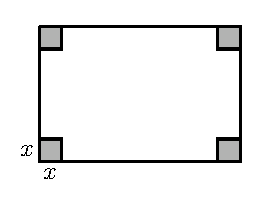
\includegraphics{box}\end{center}
%\end{question}
%\begin{answer}$x=\dfrac{5-\sqrt{7}}{2}\approx 1.18$
%\end{answer}
%\begin{solution} The box has height $x$ and base $(6-2x)\times(9-2x)$.
%So the box has volume $x(6-2x)(9-2x)=54x-30x^2+4x^3$. This volume is a maximum %when
%$$
%0=\diff{}{x}(54x-30x^2+4x^3)=54-60x+12 x^2
%=6(9-10x+2x^2)
%\implies x=\dfrac{10\pm\sqrt{100-4\times2\times 9}}{4}
%$$
%Since $x$ runs from 0 to 3 (at which point the short dimension of the base has
%shrunk to zero) and both $x=0$ and $x=3$ give volume zero, the maximum
%must be achieved by one of $\dfrac{10\pm\sqrt{100-72}}{4}
%=\dfrac{10\pm\sqrt{28}}{4}=\dfrac{10\pm2\sqrt{7}}{4}
%=\dfrac{5\pm\sqrt{7}}{2}$. The plus sign,
%$\dfrac{5+\sqrt{7}}{2}\approx 3.8$ is outside the allowed range for $x$,
%the maximum is given by \boxed{x=\dfrac{5-\sqrt{7}}{2}\approx 1.18}$\,$.
%\end{solution}

%%%%%
\section{Sketching Graphs}
\subsection{Domain, intercepts and asymptotes}
%
% Copyright 2018 Joel Feldman, Andrew Rechnitzer and Elyse Yeager.
% This work is licensed under a Creative Commons Attribution-NonCommercial-ShareAlike 4.0 International License.
% https://creativecommons.org/licenses/by-nc-sa/4.0/
%
\questionheader{ex:s3.6.1}
%%%%%%%%%%%%%%%%%%
\subsection*{\Conceptual}
%%%%%%%%%%%%%%%%%%

\begin{Mquestion}
Suppose $f(x)$ is a function given by
\[f(x)= \frac{g(x)}{x^2-9}\]
where $g(x)$ is also a function. True or false: $f(x)$ has a vertical asymptote at $x=-3$.
\end{Mquestion}
\begin{hint}
What happens if $g(x)=x+3$?
\end{hint}
\begin{answer}
In general, false.
\end{answer}
\begin{solution}
In general, this is false. For example, the function $f(x) = \dfrac{x^2-9}{x^2-9}$ has no vertical asymptotes, because it is equal to 1 in every point in its domain (and is undefined when $x=\pm3$).

However, it is certainly \emph{possible} that $f(x)$ has a vertical asymptote at $x=-3$. For example, $f(x)=\dfrac{1}{x^2-9}$ has a vertical asymptote at $x=-3$.  More generally, if $g(x)$ is continuous and $g(-3)\ne 0$,
          then $f(x)$ has a vertical asympotote at $x=-3$.
\end{solution}
%%%%%%%%%%%%%%%%%%
\subsection*{\Procedural}
%%%%%%%%%%%%%%%%%%


\begin{Mquestion}
Match the functions $f(x)$, $g(x)$, $h(x)$, and $k(x)$ to the curves $y=A(x)$ through $y=D(x)$.
\begin{center}
$f(x)=\sqrt{x^2+1}$\hfill
$g(x)=\sqrt{x^2-1}$\hfill
$h(x)=\sqrt{x^2+4}$\hfill
$k(x)=\sqrt{x^2-4}$

\begin{tikzpicture}
\YEaaxis{3}{3}{1}{4}
\draw[thick, orange] plot[domain=-3:3, samples=100](\x,{sqrt(\x*\x+1)}) node[right]{$y=A(x)$};
\foreach \x in {1,-1,2,-2}{\YExcoord{\x}{\x}}
\foreach \x in {1,2}{\YEycoord{\x}{\x}}
\end{tikzpicture}
\hfill
\begin{tikzpicture}
\YEaaxis{3}{3}{1}{4}
\draw[thick, red] plot[domain=-3:3, samples=100](\x,{sqrt(\x*\x+4)}) node[right]{$y=B(x)$};
\foreach \x in {1,-1,2,-2}{\YExcoord{\x}{\x}}
\foreach \x in {1,2}{\YEycoord{\x}{\x}}
\end{tikzpicture}

\begin{tikzpicture}
\YEaaxis{3}{3}{1}{4}
\draw[thick, blue] plot[domain=-3:-1, samples=100](\x,{sqrt(\x*\x-1)});
\draw[thick, blue] plot[domain=1:3, samples=100](\x,{sqrt(\x*\x-1)})node[right]{$y=C(x)$};
\foreach \x in {1,-1,2,-2}{\YExcoord{\x}{\x}}
\foreach \x in {1,2}{\YEycoord{\x}{\x}}
\end{tikzpicture}
\hfill
\begin{tikzpicture}
\YEaaxis{3}{3}{1}{4}
\draw[thick, green!80!black] plot[domain=-3:-2, samples=100](\x,{sqrt(\x*\x-4)});
\draw[thick, green!80!black] plot[domain=2:3, samples=100](\x,{sqrt(\x*\x-4)}) node[right]{$y=D(x)$};
\foreach \x in {1,-1,2,-2}{\YExcoord{\x}{\x}}
\foreach \x in {1,2}{\YEycoord{\x}{\x}}
\end{tikzpicture}
\end{center}
\end{Mquestion}
\begin{hint}
Use domains and intercepts to distinguish between the functions.
\end{hint}
\begin{answer}
\textcolor{orange}{$f(x)=A(x)$}
\qquad
\textcolor{blue}{$g(x)=C(x)$}
\qquad
\textcolor{red}{$h(x)=B(x)$}
\qquad
\textcolor{green!90!black}{$k(x)=D(x)$}
\end{answer}
\begin{solution}
Since $x^2+1$ and $x^2+4$ are always positive, $f(x)$ and $h(x)$ are defined over all real numbers. So, $f(x)$ and $h(x)$ correspond to $A(x)$ and $B(x)$. Which is which? $A(0)=1=f(0)$ while $B(0)=2=h(0)$, so \textcolor{orange}{$A(x)=f(x)$} and
\textcolor{red}{$B(x)=h(x)$}.

That leaves $g(x)$ and $k(x)$ matching to $C(x)$ and $D(x)$. The domain of $g(x)$ is all $x$ such that $x^2-1\ge0$. That is, $|x|\ge1$, like $C(x)$.
The domain of $k(x)$ is all $x$ such that $x^2-4\ge0$. That is, $|x|\ge2$, like $D(x)$.
So, \textcolor{blue}{$C(x)=g(x)$} and \textcolor{green}{$D(x)=k(x)$}.
\end{solution}

\begin{Mquestion}
Below is the graph of
\[y=f(x)=\sqrt{\log^2(x+p)}\]
\begin{enumerate}[(a)]
\item What is $p$?
\item What is $b$ (marked on the graph)?
\item What is the $x$-intercept of $f(x)$?
\end{enumerate}
Remember $\log(x+p)$ is the natural logarithm of $x+p$, $\log_e(x+p)$.

\begin{center}
\begin{tikzpicture}
\YEaaxis{9}{3}{1}{5}
\draw[thick, red] plot[domain=-7.38:2, samples=200](\x,{sqrt(ln(\x+7.39)*ln(\x+7.39))});
\draw[dashed] (-7.39,5)--(-7.39,-.2) node[below]{$b$};
\foreach \y in {1,2,3}{\YEycoord{\y}{\y}}
\foreach \x in {-6,...,-1}{\YExcoord{\x}{\x}}
\foreach \x in {1,2,-8}{\YExcoord{\x}{\x}}
\end{tikzpicture}
\end{center}
\end{Mquestion}
\begin{hint}
To find $p$, the equation $f(0)=2$ gives you two possible values of $p$. Consider the domain of $f(x)$ to decide between them.
\end{hint}
\begin{answer}
(a) $p=e^2$ \qquad (b) $b=-e^2$ \qquad $1-e^2$
\end{answer}
\begin{solution}
(a) Since $f(0)=2$, we solve
\begin{align*}
2&=\sqrt{\log^2(0+p)}\\
&=\sqrt{\log^2 p}\\
&=\left|\log p\right|\\
\log p &= \pm 2\\
p&=e^{\pm 2}\\
p&=e^2 \mbox{ or } p=\frac{1}{e^2}
\end{align*}
We know that $p$ is $e^2$ or $\dfrac{1}{e^2}$, but we have to decide between the two. In both cases, $f(0)=2$. Let's consider the domain of $f(x)$. Since $\log^2(x+p)$ is never negative, the square root does not restrict our domain. However, we can only take the logarithm of positive numbers. Therefore, the domain is
\begin{align*}
x \mbox{ such that } &x+p>0\\
x \mbox{ such that } &x>-p\\
\end{align*}
If $p=\dfrac{1}{e^2}$, then the domain of $f(x)$ is $\left(-\dfrac{1}{e^2},\infty\right)$. In particular, since $-\dfrac{1}{e^2}>-1$, the domain of $f(x)$ does not include $x=-1$. However, it is clear from the graph that $f(-1)$ exists. So, $p=e^2$.

(b) Now, we need to figure out what $b$ is.
Notice that $b$ is the end of the domain of $f(x)$, which we already found to be $(-p,\infty)$. So, $b=-p=-e^2$.

 (As a quick check, if we take $e\approx 2.7$, then $-e^2=-7.29$, and this looks about right on the graph.)

 (c) The $x$-intercept is the value of $x$ for which $f(x)=0$:
 \begin{align*}
 0&=\sqrt{\log^2(x+p)}\\
 0&=\log(x+p)\\
 1&=x+p\\
 x&=1-p=1-e^2
 \end{align*}
 The $x$-intercept is $1-e^2$.

 (As another quick check, the $x$-intercept we found is a distance of 1 from the vertical asymptote, and this looks about right on the graph.)
\end{solution}


\begin{Mquestion}
Find all asymptotes of $f(x)=\dfrac{x(2x+1)(x-7)}{3x^3-81}$.
\end{Mquestion}
\begin{hint}
Check for horizontal asymptotes by evaluating $\ds\lim_{x \to \pm \infty}f(x)$, and
check for vertical asymptotes by finding any value of $x$ near which $f(x)$ blows up.
\end{hint}
\begin{answer}
 vertical asymptote at $x=3$; horizontal asymptotes $\ds\lim_{x \to \pm \infty}f(x)=\dfrac{2}{3}$
\end{answer}
\begin{solution}
Vertical asymptotes occur where the function blows up. In rational functions, this can only happen when the denominator goes to 0. In our case, the denominator is 0 when $x=3$, and in this case the numerator is $147$. That means that as $x$ gets closer and closer to 3, the numerator gets closer and closer to 147 while the denominator gets closer and closer to 0, so $|f(x)|$ grows without bound. That is, there is a vertical asymptote at $x=3$.

The horizontal asymptotes are found by taking the limits as $x$ goes to infinity and negative infinity. In our case, they are the same, so we condense our work.
\begin{align*}
\lim_{x \to \pm \infty}\dfrac{x(2x+1)(x-7)}{3x^3-81}
&=\lim_{x \to \pm \infty}\dfrac{2x^3+ax^2+bx+c}{3x^3-81}
\intertext{where $a$, $b$, ad $c$ are some constants. Remember, for rational functions, you can figure out the end behaviour by looking only at the terms with the highest degree--the others won't matter, so we don't bother finding them. From here, we  divide the numerator and denominator by the highest power of $x$ in the denominator, $x^3$.}
&=\lim_{x \to \pm \infty}\dfrac{2x^3+ax^2+bx+c}{3x^3-81}\left(\frac{\tfrac{1}{x^3}}{\tfrac{1}{x^3}}\right)\\
&=\lim_{x \to \pm \infty}\dfrac{2+\tfrac{a}{x}+\tfrac{b}{x^2}+\tfrac{c}{x^3}}{3-\tfrac{81}{x^3}}\\
&=\dfrac{2+0+0+0}{3-0}=\frac{2}{3}
\end{align*}
So there is a horizontal asymptote of $y=\dfrac{2}{3}$ both as $x \to \infty$ and as $x \to -\infty$.
\end{solution}

\begin{question}
Find all asymptotes of $f(x)=10^{3x-7}$.
\end{question}
\begin{hint}
Check for horizontal asymptotes by evaluating $\ds\lim_{x \to \pm \infty}f(x)$, and
check for vertical asymptotes by finding any value of $x$ near which $f(x)$ blows up.
\end{hint}
\begin{answer}
horizontal asymptote $y=0$ as $x \to -\infty$; no other asymptotes
\end{answer}
\begin{solution}
Since $f(x)$ is continuous over all real numbers, it has no vertical asymptote.

To find the horizontal asymptotes, we evaluate
$\ds\lim_{x \to \pm \infty}f(x)$.
\begin{align*}
\lim_{x \to \infty}10^{3x-7}&=\underbrace{\lim_{X \to \infty}10^X}_{\mbox{let }X=3x-7}=\infty
\intertext{So, there's no horizontal asymptote as $x \to \infty$.}
\lim_{x \to -\infty}10^{3x-7}&=\underbrace{\lim_{X \to -\infty}10^{X}}_{\mbox{let }X=3x-7}\\
&=\underbrace{\lim_{X' \to \infty}10^{-X'}}_{\mbox{let }X'=-X}\\
&=\lim_{X' \to \infty}\frac{1}{10^{X'}}\\
&=0
\end{align*}
That is, $y=0$ is a horizontal asymptote as $x \to -\infty$.
\end{solution}

\subsection{First derivative - increasing or decreasing}
%
% Copyright 2018 Joel Feldman, Andrew Rechnitzer and Elyse Yeager.
% This work is licensed under a Creative Commons Attribution-NonCommercial-ShareAlike 4.0 International License.
% https://creativecommons.org/licenses/by-nc-sa/4.0/
%
\questionheader{ex:s3.6.2}
%%%%%%%%%%%%%%%%%%
\subsection*{\Conceptual}
%%%%%%%%%%%%%%%%%%

\begin{Mquestion}
Match each function graphed below to its \emph{derivative} from the list. (For example, which function on the list corresponds to $A'(x)$?)

The $y$-axes have been scaled to make the curve's behaviour clear, so the vertical scales differ from graph to graph.

\begin{center}
$l(x)=(x-2)^4$
\qquad
$m(x)=(x-2)^4(x+2)$
\qquad
$n(x)=(x-2)^2(x+2)^2$
\qquad
$o(x)=(x-2)(x+2)^3$
\qquad
$p(x)=(x+2)^4$

\begin{tikzpicture}[scale=0.9]
\YEaaxis{3}{4}{3}{3}
\draw[thick, green!80!black] plot[domain=-1.5:4, samples=100](\x,{(\x-2)*(\x-2)*(\x-2)*(\x-2)*(\x-2)/100+2}) node[above right]{$y=A(x)$};
\foreach \x in {2,-2}{\YExcoord{\x}{\x}}
\end{tikzpicture}
%
\begin{tikzpicture}[scale=0.9]
\YEaaxis{4}{3}{3}{3}
\draw[thick, blue] plot[domain=-4:1.5, samples=100](\x,{(\x+2)*(\x+2)*(\x+2)*(\x+2)*(\x+2)/100-2}) node[above right]{$y=B(x)$};
\foreach \x in {2,-2}{\YExcoord{\x}{\x}}
\end{tikzpicture}

\begin{tikzpicture}
\YEaaxis{3}{3}{3}{3}
\draw[thick, red] plot[domain=-3:3, samples=100](\x,{(-.8*\x*\x*\x*\x*\x+16/3*\x*\x*\x+(\x*\x-4*\x+4)*(\x*\x+4*\x+4)*\x)/10}) node[right]{$y=C(x)$};
\foreach \x in {2,-2}{\YExcoord{\x}{\x}}
\end{tikzpicture}

\begin{tikzpicture}[scale=0.8]
\YEaaxis{3.5}{3}{3}{3}
\draw[thick, orange] plot[domain=-4:3.1, samples=100](\x,{1/75*(\x-3)*(\x+2)*(\x+2)*(\x+2)*(\x+2)+1}) node[above right]{$y=D(x)$};
\foreach \x in {2,-2}{\YExcoord{\x}{\x}}
\end{tikzpicture}
%
\begin{tikzpicture}[scale=0.8]
\YEaaxis{3}{4}{3}{3}
\draw[thick, purple] plot[domain=-2.6:3.75, samples=100](\x,{1/900*(\x-2)*(\x-2)*(\x-2)*(\x-2)*(\x-2)*(5*\x+14)+1.5}) node[above right]{$y=E(x)$};
\foreach \x in {2,-2}{\YExcoord{\x}{\x}}
\end{tikzpicture}

\end{center}
\end{Mquestion}
\begin{hint}
For each of the graphs, consider where the derivative is positive, negative, and zero.
\end{hint}
\begin{answer}
$\textcolor{green}{A'(x)=l(x)} \qquad \textcolor{blue}{B'(x)=p(x)}
\qquad
\textcolor{red}{C'(x)=n(x)}
\qquad
\textcolor{orange}{D'(x)=o(x)}\qquad \textcolor{purple}{E'(x)=m(x)}$
\end{answer}
\begin{solution}
Functions $A(x)$ and $B(x)$ share something in common that sets them apart from the others: they have a horizontal tangent line only once. In particular, $A'(-2) \neq 0$ and $B'(2) \neq 0$. The only listed functions that do not have two distinct roots are $l(x)$ and $p(x)$. Since $l(-2) \neq 0$ and $p(2) \neq 0$, we conclude
\[\textcolor{green}{A'(x)=l(x)} \qquad \textcolor{blue}{B'(x)=p(x)}\]

Function $C(x)$ is never decreasing. Its tangent line is horizontal when $x = \pm 2$, but the curve never decreases, so $C'(x) \geq 0$ for all $x$ and $C'(2)=C'(-2)=0$. The only function that matches this is $n(x)=(x-2)^2(x+2)^2$. Since its linear terms have even powers, it is never negative, and its roots are precisely $x=\pm 2$.
\[\textcolor{red}{C'(x)=n(x)}\]

For the functions $D(x)$ and $E(x)$ we consider their behaviour
          near $x=0$.  $D(x)$ is decreasing near $x=0$, so $D'(0)<0$, which matches with $o(0)<0$. Contrastingly, $E(x)$ is increasing near zero, so
          $E'(0)>0$, which matches with $m(0)>0$.
\[\textcolor{orange}{D'(x)=o(x)}\qquad \textcolor{purple}{E'(x)=m(x)}\]
\end{solution}


%%%%%%%%%%%%%%%%%%
\subsection*{\Procedural}
%%%%%%%%%%%%%%%%%%


\begin{question}[2015Q]
Find the interval(s) where $f(x)=\dfrac{e^x}{x+3}$ is increasing.
\end{question}
\begin{hint}
Where is $f'(x)>0$?
\end{hint}
\begin{answer}
$(-2,\infty)$
\end{answer}
\begin{solution}
The domain of $f(x)$ is all real numbers except $-3$ (because when $x=-3$ the denominator is zero). For $x\neq -3$, we differentiate using the quotient rule:
$$f'(x)=\frac{e^x(x+3) - e^x(1)}{(x+3)^2} = \frac{e^x}{(x+3)^2} (x+2)\,.$$
Since $e^x$ and $(x+3)^2$ are  positive for every $x$ in the domain of $f(x)$, the sign of $f'(x)$ is the same as the sign of $x+2$. We conclude that $f(x)$
is increasing for every $x$ in its domain with $x+2>0$. That is, over the interval $(-2,\infty)$.
\end{solution}




\begin{question}[2015Q] Find the interval(s) where $f(x)=\dfrac{\sqrt{x-1}}{2x+4}$ is increasing.
\end{question}
\begin{hint}
Consider the signs of the numerator and the denominator of $f'(x)$.
\end{hint}
\begin{answer}
$(1,4)$ and $[1,4)$ are both acceptable answers
\end{answer}
\begin{solution}
Since we can't take the square root of a negative number,  $f(x)$ is only defined
when $x \ge 1$. Furthermore, since we can't have a zero as a denominator, $x=-2$ is  not in the domain--but as long as $x \ge 1$, also $x \ne -2$. So, the domain of the function is $[1,\infty)$.

 In order to find where is $f(x)$ increasing, we find where is $f'(x)$ positive.
$$f'(x)=\frac{\frac{2x+4}{2\sqrt{x-1}}-2\sqrt{x-1}}{(2x+4)^2}=\frac{(x+2)-2(x-1)}{\sqrt{x-1}(2x+4)^2}
=\frac{-x+4}{\sqrt{x-1}(2x+4)^2}$$
The denominator is never negative, so  $f(x)$ is increasing when the numerator of $f'(x)$ is positive, i.e. when $4-x>0$, or $x<4$. Recalling that the domain of definition for $f(x)$ is $[1,+\infty)$, we conclude that $f(x)$ is increasing on the interval $(1,4)$.

Remark: $[1,4)$ is also an acceptable answer, but $[1,4]$ is not. At $x=4$ the function has a local maximum: $f(x)$ is increasing before $x=4$ and decreasing after.
\end{solution}


\begin{Mquestion}[2015Q]
Find the interval(s) where $f(x)=2\arctan (x) - \log(1+x^2)$ is increasing.
\end{Mquestion}
\begin{hint}
Remember $\ds\diff{}{x}\{\arctan x\}=\dfrac{1}{1+x^2}$.
\end{hint}
\begin{answer} $(-\infty,1)$
\end{answer}
\begin{solution}
The domain of arctangent is all real numbers. The domain of the logarithm function is all positive numbers, and $1+x^2$ is positive for all $x$. So, the domain of $f(x)$ is all real numbers.

In order to find where is $f(x)$ increasing, we find where is $f'(x)$ positive.
$$f'(x)= \frac 2 {1+x^2} - \frac{2x}{1+x^2} = \frac{2-2x}{1+x^2}$$
Since the denominator is always positive, $f(x)$ is increasing
when when $2-2x>0$.We conclude that $f(x)$ is increasing on the interval $(-\infty,1)$.
\end{solution}

\subsection{Second derivative - concavity}
%
% Copyright 2018 Joel Feldman, Andrew Rechnitzer and Elyse Yeager.
% This work is licensed under a Creative Commons Attribution-NonCommercial-ShareAlike 4.0 International License.
% https://creativecommons.org/licenses/by-nc-sa/4.0/
%
\questionheader{ex:s3.6.3}


%%%%%%%%%%%%%%%%%%
\subsection*{\Conceptual}
%%%%%%%%%%%%%%%%%%

\begin{Mquestion}
On the graph below, mark the intervals where $f''(x)>0$ (i.e. $f(x)$ is concave up) and where $f''(x)<0$ (i.e. $f(x)$ is concave down).
\begin{center}
\begin{tikzpicture}
\YEaxis{6}{4}
\draw[thick] plot[domain=-6:-2](\x,{exp(\x+2)+1});
\draw[thick] plot[domain=-2:4](\x,{cos(\x*.785 r)+2});
\draw[thick] plot[domain=0:2](\x+4,{3*cos(\x*.785 r)-2});
\end{tikzpicture}
\end{center}
\end{Mquestion}
\begin{hint}
There are two intervals where the function is concave up, and two where it is concave down.
\end{hint}
\begin{answer}
\begin{center}
\begin{tikzpicture}
\YEaxis{6}{4}
\draw[thick, red] plot[domain=-6:-2](\x,{exp(\x+2)+1});
\draw[thick, blue] plot[domain=-2:2](\x,{cos(\x*.785 r)+2});
\draw[thick, red] plot[domain=2:4](\x,{cos(\x*.785 r)+2});
\draw[thick, blue] plot[domain=0:2](\x+4,{3*cos(\x*.785 r)-2});
\draw[thick, red, decorate, decoration={brace, amplitude=10pt, mirror}]
(-6,0)--(-2,0);
\draw[red] (-4,-1) node{concave up};
\draw[thick, blue, decorate, decoration={brace, amplitude=10pt, mirror}]
(-2,0)--(2,0);
\draw[blue] (0,-1) node{concave down};
\draw[thick, red, decorate, decoration={brace, amplitude=10pt, mirror}]
(2,0)--(4,0);
\draw[red] (3,-1) node{concave up};
\draw[thick, blue, decorate, decoration={brace, amplitude=10pt}]
(4,2)--(6,2);
\draw[blue] (5,2.75) node{concave down};
\end{tikzpicture}
\end{center}
\end{answer}
\begin{solution}
\begin{center}
\begin{tikzpicture}
\YEaxis{6}{4}
\draw[thick, red] plot[domain=-6:-2](\x,{exp(\x+2)+1});
\draw[thick, blue] plot[domain=-2:2](\x,{cos(\x*.785 r)+2});
\draw[thick, red] plot[domain=2:4](\x,{cos(\x*.785 r)+2});
\draw[thick, blue] plot[domain=0:2](\x+4,{3*cos(\x*.785 r)-2});
\draw[thick, red, decorate, decoration={brace, amplitude=10pt, mirror}]
(-6,0)--(-2,0);
\draw[red] (-4,-1) node{concave up};
\draw[thick, blue, decorate, decoration={brace, amplitude=10pt, mirror}]
(-2,0)--(2,0);
\draw[blue] (0,-1) node{concave down};
\draw[thick, red, decorate, decoration={brace, amplitude=10pt, mirror}]
(2,0)--(4,0);
\draw[red] (3,-1) node{concave up};
\draw[thick, blue, decorate, decoration={brace, amplitude=10pt}]
(4,2)--(6,2);
\draw[blue] (5,2.75) node{concave down};
\end{tikzpicture}
\end{center}
In the graph above, the concave-up sections are marked in red. These are where the graph has an increasing derivative; equivalently, where the graph lies above its tangent lines; more descriptively, where it curves like a smiley face.

Concave-down sections are marked in blue. These are where the graph has a decreasing derivative; equivalently, where the graph lies below its tangent lines; more descriptively, where it curves like a frowney face.
\end{solution}



\begin{Mquestion}
Sketch a curve that is:
\begin{itemize}
\item concave up when $|x|>5$,
\item concave down when $|x|<5$,
\item increasing when $x<0$, and
\item decreasing when $x>0$.
\end{itemize}
\end{Mquestion}
\begin{hint}
Try allowing your graph to have horizontal asymptotes. For example, let the function get closer and closer to the $x$-axis (or another horizontal line) without touching it.
\end{hint}
\begin{answer}
\begin{center}
\begin{tikzpicture}
\YEaaxis{6}{6}{1}{4}
\draw[thick] plot[domain=-3:0] (\x-3,{exp(\x)});
\draw[thick] plot[domain=0:3] (\x+3,{exp(-\x)});
\draw[thick] plot[domain=-3:3] (\x,{cos(\x*0.523 r)/0.523+1});
\YExcoord{-3}{-5}
\YExcoord{3}{5}
\end{tikzpicture}
\end{center}
\end{answer}
\begin{solution}
The most basic shape of the graph is given by the last two bullet points:
\begin{center}
\begin{tikzpicture}
\YEaaxis{6}{6}{1}{4}
\draw[thick, <->] (-6,1)--(0,3)--(6,1);
\YExcoord{-3}{-5}
\YExcoord{3}{5}
\end{tikzpicture}
\end{center}
The curve is concave down over the interval $(-5,5)$, so let's give it a frowney-face curvature there.
\begin{center}
\begin{tikzpicture}
\YEaaxis{6}{6}{1}{4}
\draw[thick] plot[domain=-3:3] (\x,{cos(\x*0.523 r)/0.523+1});
\draw[thick] (-6,-.25)--(-3,1) (3,1)--(6,-.25);
\YExcoord{-3}{-5}
\YExcoord{3}{5}
\end{tikzpicture}
\end{center}
Finally, when $x>5$ or $x<-5$, our curve should be concave up, so let's give it smiley-face curvature there, without changing its basic increasing/decreasing shape.
\begin{center}
\begin{tikzpicture}
\YEaaxis{6}{6}{1}{4}
\draw[thick] plot[domain=-3:0] (\x-3,{exp(\x)});
\draw[thick] plot[domain=0:3] (\x+3,{exp(-\x)});
\draw[thick] plot[domain=-3:3] (\x,{cos(\x*0.523 r)/0.523+1});
\YExcoord{-3}{-5}
\YExcoord{3}{5}
\end{tikzpicture}
\end{center}
This finishes our sketch.
\end{solution}


\begin{question}\label{s3.6.3converse}
Suppose $f(x)$ is a function whose second derivative exists and is continuous for all real numbers.

True or false: if $f''(3)=0$, then $x=3$ is an inflection point of $f(x)$.

Remark: compare to Question~\ref{s3.6.3IVT}
\end{question}
\begin{hint}
Consider $f(x)=(x-3)^4$.
\end{hint}
\begin{answer}
In general, false.
\end{answer}
\begin{solution}
An inflection point is where the concavity of a function changes. It is possible that $x=3$ is an inflection point, but it is also possible that is not. So, the statement is false, in general.

For example, let $f(x)=(x-3)^4$. Since $f(x)$ is a polynomial, all its derivatives exist and are continuous. $f''(x)=12(x-3)^2$, so $f(3)=0$. However, since $f''(x)$ is something squared, it is never negative, so $f(x)$ is never concave down. Since $f(x)$ is never concave down, it never changes concavity, so it has no inflection points.

Remark: finding inflection points is somewhat reminiscent of finding local extrema. To find local extrema, we first find all critical and singular points, since local extrema can only occur there. Then, we have to figure out which critical and singular points are actually local extrema. Similarly, if you want to find inflection points, start by finding where $f''(x)$ is zero or non-existant, because inflection points can only occur there (see Question~\ref{s3.6.3IVT}). Then, you still have to check whether those points are actually inflection points.
\end{solution}
%%%%%%%%%%%%%%%%%%
\subsection*{\Procedural}
%%%%%%%%%%%%%%%%%%


\begin{Mquestion}[1997D]
Find all inflection points for the graph of $f(x)=3x^5-5x^4+13x$.
\end{Mquestion}
\begin{answer}
$x=1,\ y=11$
\end{answer}
\begin{solution}
Inflection points occur where $f''(x)$ changes sign. Since $f(x)$ is a polynomial, its first and second derivatives exist everywhere, and are themselves polynomials. In particular,
\begin{align*}f(x)&=3x^5-5x^4+13x\\
f'(x)&=15x^4-20x^3+13\\
f''(x)&=60x^3-60x^2=60x^2(x-1)
\end{align*}
The second derivative is negative for $x<1$ and positive for $x>1$. Thus
the concavity changes between concave up and concave down at
{$x=1,\ y=11$}.

This is the only inflection point. It is true that $f''(0)=0$, but for values of $x$ both a little larger than and a little smaller than 0, $f''(x)<0$, so the concavity does not change at $x=0$.
\end{solution}


%%%%%%%%%%%%%%%%%%
\subsection*{\Application}
%%%%%%%%%%%%%%%%%%

\Instructions{Questions~\ref{s3.6.3proof1} through \ref{s3.6.3IVT} ask you to show that certain things are true. Give a clear explanation using concepts and theorems from this semester.}

\begin{Mquestion}[1997A]\label{s3.6.3proof1}
Let
\[f(x)=\frac{x^5}{20}+\frac{5x^3}{6}-10x^2+500x+1000\]
Show that $f(x)$ has exactly one inflection point.
\end{Mquestion}
\begin{hint}
You must show it has at least one inflection point (try the Intermediate Value Theorem), and at most one inflection point (consider whether the second derivative is increasing or decreasing).
\end{hint}
\begin{answer}
Let \[g(x)=f''(x)=x^3+5x-20.\] Then $g'(x)=3x^2+5$, which is always positive. That means $g(x)$ is strictly increasing for all $x$. So, $g(x)$ can change signs once, from negative to positive, but it can never change back to negative. An inflection point of $f(x)$ occurs when $g(x)$ changes signs. So, $f(x)$ has \emph{at most one} inflection point.

Since $g(x)$ is continuous, we can apply the Intermediate Value Theorem to it. Notice
$g(3)>0$ while $g(0)<0$. By the IVT, $g(x)=0$ for at least one $x \in (0,3)$. Since $g(x)$ is strictly increasing, at the point where $g(x)=0$, $g(x)$ changes from negative to positive. So, the concavity of $f(x)$ changes. Therefore, $f(x)$ has \emph{at least one} inflection point.

Now that we've shown that $f(x)$ has at most one inflection point, and at least one inflection point, we conclude it has exactly one inflection point.\end{answer}
\begin{solution}
In order to show that $f(x)$ has \emph{exactly one} inflection point, we will show that is has \emph{at least one}, and \emph{no more than one}.

Let \[g(x)=f''(x)=x^3+5x-20.\] Then $g'(x)=3x^2+5$, which is always positive. That means $g(x)$ is strictly increasing for all $x$. So, $g(x)$ can change signs once, from negative to positive, but it can never change back to negative. An inflection point of $f(x)$ occurs when $g(x)$ changes signs. So, $f(x)$ has at most one inflection point. (At this point, we don't know that $f(x)$ has any inflection points: maybe $g(x)$ is always positive.)

Since $g(x)$ is continuous, we can apply the Intermediate Value Theorem to it. Notice
$g(3)>0$ while $g(0)<0$. By the IVT, $g(x)=0$ for at least one $x \in (0,3)$. Since $g(x)$ is strictly increasing, at the point where $g(x)=0$, $g(x)$ changes from negative to positive. So, the concavity of $f(x)$ changes. Therefore, $f(x)$ has at least one inflection point.

Now that we've shown that $f(x)$ has at most one inflection point, and at least one inflection point, we conclude it has exactly one inflection point.
\end{solution}



\begin{Mquestion}[1996D]
Let $f(x)$ be a function whose first two derivatives exist everywhere, and $f''(x)>0$ for all $x$.
\begin{enumerate}[(a)]
 \item\label{s3.6interval1} Show that $f(x)$ has at most one critical point and that any critical point is an absolute minimum for $f(x)$.
  \item\label{s3.6interval2} Show that the maximum value of $f(x)$ on any finite interval
occurs at one of the endpoints of the interval.
\end{enumerate}
\end{Mquestion}
\begin{hint}
Use \eqref{s3.6interval1} in
proving \eqref{s3.6interval2}.
\end{hint}
\begin{answer}
\eqref{s3.6interval1}
Let
\[g(x)=f'(x)\]
Then $f''(x)$ is the derivative of $g(x)$. Since $f''(x)>0$ for all $x$, $g(x)=f'(x)$ is strictly increasing
for all $x$.
In other words, if $y>x$ then $g(y)>g(x)$.

Suppose $g(x)=0$. Then for every $y$ that is larger than $x$, $g(y)>g(x)$, so $g(y) \neq 0$. Similarly, for every $y$ that is smaller than $x$, $g(y)<g(x)$, so $g(y) \neq 0$. Therefore, $g(x)$ can only be zero for at most one value of $x$. Since $g(x)=f'(x)$, that means $f(x)$ can have at most one critical point.

Suppose $f'(c)=0$. Since
$f'(x)$ is a strictly increasing function, $f'(x)<0$ for all $x<c$ and $f'(x)>0$ for all $x>c$.
\begin{center}\begin{tikzpicture}
\draw[ultra thick, <->] (-4,0)--(4,0);
\YExcoord{0}{c}
\draw[blue, decorate, decoration={brace, mirror, amplitude=10pt}] (-4.1,-.75)--(0,-.75);
\draw[blue] (-2,-1.5) node{$x<c$, so};
\draw[blue] (-2,-2) node{$f'(x)<f'(c)=0$};
\draw[red, decorate, decoration={brace, amplitude=10pt}] (4.1,-.75)--(0,-.75);
\draw[red] (2,-1.5) node{$x>c$, so};
\draw[red] (2,-2) node{$f'(x)>f'(c)=0$};
\end{tikzpicture}\end{center}

Then $f(x)$ is decreasing for $x<c$ and increasing for $x>c$.
So $f(x)>f(c)$ for all $x\neq c$.

\begin{center}\begin{tikzpicture}
\draw[ultra thick, <->] (-4,0)--(4,0);
\YExcoord{0}{c}
\draw[blue, decorate, decoration={brace, mirror, amplitude=10pt}] (-4.1,-.75)--(0,-.75);
\draw[blue] (-2,-1.5) node{$f(x)$ decreasing, so};
\draw[blue] (-2,-2) node{$f(x)>f(c)$};
\draw[red, decorate, decoration={brace, amplitude=10pt}] (4.1,-.75)--(0,-.75);
\draw[red] (2,-1.5) node{$f(x)$ increasing, so};
\draw[red] (2,-2) node{$f(x)>f(c)$};
\draw[thick, dashed] (-4,3)--(0,1)--(4,3) node[right]{$y=f(x)$};
\draw[blue] (-2,2) node[vertex]{};
\draw (0,1) node[vertex]{};
\draw[red] (2,2) node[vertex]{};
\color{blue}\YExcoord{-2}{x<c}
\color{red}\YExcoord{2}{x>c}
\end{tikzpicture}\end{center}
 Since $f(x)>f(c)$ for
all $x\ne c$, so $c$ is an absolute minimum for $f(x)$.

\eqref{s3.6interval2}
We know that the maximum over an interval occurs at an endpoint,
a critical point, or a singular point.
\begin{itemize}
\item  Since $f'(x)$ exists everywhere, there are no singular points.
\item If the maximum were achieved at a critical point, that critical point would
have to provide both the absolute maximum and the absolute minimum (by part (a)).
So, the function would have to be a constant and consequently could not have
a nonzero second derivative. So the maximum is not at a critical point.
\end{itemize}
That leaves only the endpoints of the interval.
\end{answer}
\begin{solution}
\eqref{s3.6interval1}
Let
\[g(x)=f'(x)\]
Then $f''(x)$ is the derivative of $g(x)$. Since $f''(x)>0$ for all $x$, $g(x)=f'(x)$ is strictly increasing
for all $x$.
In other words, if $y>x$ then $g(y)>g(x)$.

Suppose $g(x)=0$. Then for every $y$ that is larger than $x$, $g(y)>g(x)$, so $g(y) \neq 0$. Similarly, for every $y$ that is smaller than $x$, $g(y)<g(x)$, so $g(y) \neq 0$. Therefore, $g(x)$ can only be zero for at most one value of $x$. Since $g(x)=f'(x)$, that means $f(x)$ can have at most one critical point.

Suppose $f'(c)=0$. Since
$f'(x)$ is a strictly increasing function, $f'(x)<0$ for all $x<c$ and $f'(x)>0$ for all $x>c$.
\begin{center}\begin{tikzpicture}
\draw[ultra thick, <->] (-4,0)--(4,0);
\YExcoord{0}{c}
\draw[blue, decorate, decoration={brace, mirror, amplitude=10pt}] (-4.1,-.75)--(0,-.75);
\draw[blue] (-2,-1.5) node{$x<c$, so};
\draw[blue] (-2,-2) node{$f'(x)<f'(c)=0$};
\draw[red, decorate, decoration={brace, amplitude=10pt}] (4.1,-.75)--(0,-.75);
\draw[red] (2,-1.5) node{$x>c$, so};
\draw[red] (2,-2) node{$f'(x)>f'(c)=0$};
\end{tikzpicture}\end{center}

Then $f(x)$ is decreasing for $x<c$ and increasing for $x>c$.
So $f(x)>f(c)$ for all $x<c$ and $f(x)>f(c)$ for all $x>c$.

\begin{center}\begin{tikzpicture}
\draw[ultra thick, <->] (-4,0)--(4,0);
\YExcoord{0}{c}
\draw[blue, decorate, decoration={brace, mirror, amplitude=10pt}] (-4.1,-.75)--(0,-.75);
\draw[blue] (-2,-1.5) node{$f(x)$ decreasing, so};
\draw[blue] (-2,-2) node{$f(x)>f(c)$};
\draw[red, decorate, decoration={brace, amplitude=10pt}] (4.1,-.75)--(0,-.75);
\draw[red] (2,-1.5) node{$f(x)$ increasing, so};
\draw[red] (2,-2) node{$f(x)>f(c)$};
\draw[thick, dashed] (-4,3)--(0,1)--(4,3) node[right]{$y=f(x)$};
\draw[blue] (-2,2) node[vertex]{};
\draw (0,1) node[vertex]{};
\draw[red] (2,2) node[vertex]{};
\color{blue}\YExcoord{-2}{x<c}
\color{red}\YExcoord{2}{x>c}
\end{tikzpicture}\end{center}
 We have concluded that $f(x)>f(c)$ for
all $x\ne c$, so $c$ is an absolute minimum for $f(x)$.

\eqref{s3.6interval2}
We know that the maximum over an interval occurs at an endpoint,
at a critical point, or at a singular point.
\begin{itemize}
\item  Since $f'(x)$ exists everywhere, there are no singular points.
\item If the maximum were achieved at a critical point, that critical point would
have to provide both the absolute maximum and the absolute minimum (by part a).
So, the function would have to be a constant and consequently could not have
a nonzero second derivative. So the maximum is not at a critical point.
\end{itemize}
That leaves only the endpoints of the interval.

%Remark: The question should
%have explicitly told you that $f'$ exists everywhere -- otherwise the maximum
%need not occur at an end point! For example, $f(x)=-x^{2/3}$ has
%$f'(x)=-\frac{2}{3}x^{-1/3}$ and $f''(x)=\frac{2}{9}x^{-4/3}
%=\frac{2}{9}\big(x^{-2/3}\big)^2>0$. But $f(x)$ has its maximum at $x=0$
%because $f(0)=0$ and $f(x)=-\big(x^{1/3}\big)^2<0$ for all $x\ne 0$.
%
%\begin{center}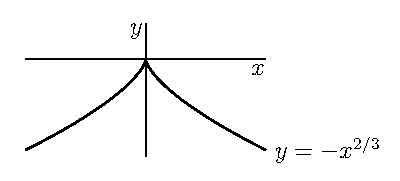
\includegraphics{graphE10}\end{center}
\end{solution}


\begin{question}\label{s3.6.3IVT}
Suppose $f(x)$ is a function whose second derivative exists and is continuous for all real numbers, and $x=3$ is an inflection point of $f(x)$. Use the Intermediate Value Theorem to show that $f''(3)=0$.

Remark: compare to Question~\ref{s3.6.3converse}.
\end{question}
\begin{hint}
Since $x=3$ is an inflection point, we know the concavity of $f(x)$ changes at $x=3$.
That is, there is some interval around 3, with endpoints $a$ and $b$, such that
\begin{itemize}
\item \textcolor{blue}{$f''(a)<0$ and $f''(x)<0$ for every $x$ between $a$ and 3,} and
\item \textcolor{red}{$f''(b)>0$ and $f''(x)>0$ for every $x$ between $b$ and 3.}
\end{itemize}
Use the IVT to show that $f''(x)=3$ for \emph{some} $x$ between $a$ and $b$; then show that this value of $x$ can't be anything \emph{except} $x=3$.
\end{hint}
\begin{answer}
If $x=3$ is an inflection point, then the concavity of $f(x)$ changes at $x=3$. That is, there is some interval strictly containing 3, with endpoints $a$ and $b$, such that
\begin{itemize}
\item \textcolor{blue}{$f''(a)<0$ and $f''(x)<0$ for every $x$ between $a$ and 3,} and
\item \textcolor{red}{$f''(b)>0$ and $f''(x)>0$ for every $x$ between $b$ and 3.}
\end{itemize}

Since $f''(a)<0$ and $f''(b)>0$, and since $f''(x)$ is continuous, the Intermediate Value Theorem tells us that there exists some $x$ strictly between $a$ and $b$ with $f''(x)=0$. So, we know $f''(x)=0$ somewhere between $a$ and $b$. The question is, where exactly could that be?

\begin{itemize}
\item $f''(x)<0$ (and hence $f''(x) \neq 0$) for all $x$ between $a$ and 3
\item $f''(x)>0$ (and hence $f''(x) \neq 0$)  for all $x$ between $b$ and 3
\item So, any number between $a$ and $b$ that is not 3 has $f''(x)\neq 0$.
\end{itemize}
So, $x=3$ is the only possible place between $a$ and $b$ where $f''(x)$ could be zero. Therefore, $f''(3)=0$.
\end{answer}
\begin{solution}
If $x=3$ is an inflection point, then the concavity of $f(x)$ changes at $x=3$. That is, there is some interval strictly containing 3, with endpoints $a$ and $b$, such that
\begin{itemize}
\item \textcolor{blue}{$f''(a)<0$ and $f''(x)<0$ for every $x$ between $a$ and 3,} and
\item \textcolor{red}{$f''(b)>0$ and $f''(x)>0$ for every $x$ between $b$ and 3.}
\end{itemize}
Remark: we are leaving unknown whether $a<3<b$ or $b<3<a$. Since we don't know whether $f(x)$ changes from concave up to concave down, or from concave down to concave up, by remaining vague we cover both cases.
\vspace{5mm}
\begin{center}
\begin{tikzpicture}
\draw[ultra thick, <->] (-4,0)--(4,0);
\YExcoord{0}{3}
\YExcoord{-3}{\textcolor{blue}{a}}
\YExcoord{3}{\textcolor{red}{b}}
\draw[decorate, decoration={brace, amplitude=10pt, mirror}, blue] (-3,-.75)--(0,-.75);
\draw[decorate, decoration={brace, amplitude=10pt, mirror}, red] (0,-.75)--(3,-.75);
\draw[blue] (-1.5,-1.5) node{concave down};
\draw[red] (1.5,-1.5) node{concave up};
\end{tikzpicture}

OR
\vspace{5mm}

\begin{tikzpicture}
\draw[ultra thick, <->] (-4,0)--(4,0);
\YExcoord{0}{3}
\YExcoord{-3}{\textcolor{red}{b}}
\YExcoord{3}{\textcolor{blue}{a}}
\draw[decorate, decoration={brace, amplitude=10pt, mirror}, red] (-3,-.75)--(0,-.75);
\draw[decorate, decoration={brace, amplitude=10pt, mirror}, blue] (0,-.75)--(3,-.75);
\draw[red] (-1.5,-1.5) node{concave up};
\draw[blue] (1.5,-1.5) node{concave down};
\end{tikzpicture}
\end{center}

Since $f''(a)<0$ and $f''(b)>0$, and since $f''(x)$ is continuous, the Intermediate Value Theorem tells us that there exists some $x$ strictly between $a$ and $b$ with $f''(x)=0$. \textcolor{red}{So, we know $f''(x)=0$ somewhere between $a$ and $b$. The question is, where exactly could that be?}


\begin{itemize}
\item $f''(x)<0$ (and hence $f''(x) \neq 0$) for all $x$ between $a$ and 3
\item $f''(x)>0$ (and hence $f''(x) \neq 0$)  for all $x$ between $b$ and 3
\item So, any number between $a$ and $b$ that is not 3 has $f''(x)\neq 0$.
\end{itemize}So, $x=3$ is the only possible place between $a$ and $b$ where $f''(x)$ could be zero. Therefore, $f''(3)=0$.

Remark: this is why, in general, we set $f''(x)=0$ to find inflection points. (They can also occur where $f''(x)$ does not exist.)
\end{solution}

\subsection{Symmetries}
%
% Copyright 2018 Joel Feldman, Andrew Rechnitzer and Elyse Yeager.
% This work is licensed under a Creative Commons Attribution-NonCommercial-ShareAlike 4.0 International License.
% https://creativecommons.org/licenses/by-nc-sa/4.0/
%
\questionheader{ex:s3.6.4}
%%%%%%%%%%%%%%%%%%
\subsection*{\Conceptual}
%%%%%%%%%%%%%%%%%%


\begin{Mquestion}
What symmetries (even, odd, periodic) does the function graphed below have?
\begin{center}\begin{tikzpicture}
\YEaxis{6}{4}
\draw plot[samples=100,domain=-1.5:1.5](3*\x,{4*(\x*\x-1)*(\x*\x-1)-2.5}) node[right]{$y=f(x)$};
\end{tikzpicture}\end{center}
\end{Mquestion}
\begin{hint}
This function is symmetric across the $y$-axis.
\end{hint}
\begin{answer}
even
\end{answer}
\begin{solution}
This function is symmetric across the $y$-axis, so it is even.
\end{solution}


\begin{question}
What symmetries (even, odd, periodic) does the function graphed below have?
\begin{center}\begin{tikzpicture}
\YEaxis{6}{4}
\draw plot[samples=100,domain=-12:12](\x/2,{2*sin(\x r)+sin(2*\x r)}) node[right]{$y=f(x)$};
\end{tikzpicture}\end{center}
\end{question}
\begin{hint}
There are two.
\end{hint}
\begin{answer}
 odd, periodic
 \end{answer}
\begin{solution}
The function is not even, because it is not mirrored across the $y$-axis.

Assuming it continues as shown, the function is periodic, because the unit shown below is repeated:
\begin{center}\begin{tikzpicture}
\YEaxis{8}{4}
\draw plot[samples=100,domain=-12:12](\x/2,{2*sin(\x r)+sin(2*\x r)}) node[right]{$y=f(x)$};
\draw[ultra thick, red] plot[samples=100,domain=0:6.28](\x/2,{2*sin(\x r)+sin(2*\x r)});
\end{tikzpicture}\end{center}

Additionally, $f(x)$ is odd. In a function with odd symmetry, if we mirror the right-hand portion of the curve (the portion to the right of the $y$-axis) across both the $y$-axis and the $x$-axis, it lines up with the left-hand portion of the curve.
\begin{center}\begin{tikzpicture}
\YEaxis{6}{4}
\draw plot[samples=100,domain=0:12](\x/2,{2*sin(\x r)+sin(2*\x r)}) node[right]{$y=f(x)$};
\draw[dashed] plot[samples=100,domain=-12:0](\x/2,{-2*sin(\x r)-sin(2*\x r)});
\draw (-3,-3) node{reflected across $y$-axis};
\end{tikzpicture}

\begin{tikzpicture}
\draw (0,1) node{};
\draw (0,-3) node{};
\draw[ultra thick, ->] (0,0)--(0,-2);
\end{tikzpicture}

\begin{tikzpicture}
\YEaxis{6}{4}
\draw plot[samples=100,domain=0:12](\x/2,{2*sin(\x r)+sin(2*\x r)}) node[right]{$y=f(x)$};
\draw[loosely dashed, gray] plot[samples=100,domain=-12:0](\x/2,{-2*sin(\x r)-sin(2*\x r)});
\draw[red, thick] plot[samples=100,domain=-12:0](\x/2,{2*sin(\x r)+sin(2*\x r)});
\draw[red] (-3,-3) node{reflected across both axes};
\end{tikzpicture}
\end{center}
Since reflecting the right-hand portion of the graph across the $y$-axis, then the $x$-axis, gives us $f(x)$, we conclude $f(x)$ is odd.
\end{solution}


\begin{question}
Suppose $f(x)$ is an even function defined for all real numbers. Below is the curve $y=f(x)$ when $x<0$. Complete the sketch of the curve.
\begin{center}\begin{tikzpicture}
\YEaxis{6}{4}
\draw plot[domain=0:6, samples=100](\x,{cos(\x r)+\x^2/12-1});
\end{tikzpicture}\end{center}
\end{question}
\begin{hint}
Since the function is even, you only have to reflect the portion shown across the $y$-axis to complete the sketch.
\end{hint}
\begin{answer}
\begin{center}\begin{tikzpicture}
\YEaxis{6}{4}
\draw plot[domain=0:6, samples=100](\x,{cos(\x r)+\x^2/12-1});
\draw plot[domain=0:6, samples=100](-\x,{cos(\x r)+\x^2/12-1});
\end{tikzpicture}\end{center}
\end{answer}
\begin{solution}
Since the function is even, we simply reflect the portion shown across the $y$-axis to complete the sketch.
\begin{center}\begin{tikzpicture}
\YEaxis{6}{4}
\draw plot[domain=0:6, samples=100](\x,{cos(\x r)+\x^2/12-1});
\draw plot[domain=0:6, samples=100](-\x,{cos(\x r)+\x^2/12-1});
\end{tikzpicture}\end{center}
\end{solution}


\begin{Mquestion}
Suppose $f(x)$ is an odd function defined for all real numbers. Below is the curve $y=f(x)$ when $x<0$. Complete the sketch of the curve.
\begin{center}\begin{tikzpicture}
\YEaxis{6}{4}
\draw plot[domain=0:6, samples=100](\x,{cos(\x r)+\x^2/12-1});
\end{tikzpicture}\end{center}
\end{Mquestion}
\begin{hint}
Since the function is odd, to complete the sketch, reflect the portion shown across the $y$-axis, then the $x$-axis.
\end{hint}
\begin{answer}
\begin{center}\begin{tikzpicture}
\YEaxis{6}{4}
\draw plot[domain=0:6, samples=100](\x,{cos(\x r)+\x^2/12-1});
\draw plot[domain=0:6, samples=100](-\x,{-cos(\x r)-\x^2/12+1});
\end{tikzpicture}\end{center}
\end{answer}
\begin{solution}
Since the function is odd, to complete the sketch, we reflect the portion shown across the $y$-axis (shown dashed), then the $x$-axis (shown in red).
\begin{center}\begin{tikzpicture}
\YEaxis{6}{4}
\draw plot[domain=0:6, samples=100](\x,{cos(\x r)+\x^2/12-1});
\draw[loosely dashed] plot[domain=0:6, samples=100](-\x,{cos(\x r)+\x^2/12-1});
\draw[red] plot[domain=0:6, samples=100](-\x,{-cos(\x r)-\x^2/12+1});
\end{tikzpicture}
\end{center}
\end{solution}

%%%%%%%%%%%%%%%%%%
\subsection*{\Procedural}
%%%%%%%%%%%%%%%%%%


\begin{Mquestion}
\[f(x)=\frac{x^4-x^6}{e^{x^2}}\]
Show that $f(x)$ is even.
\end{Mquestion}
\begin{hint}
A function is even if $f(-x)=f(x)$.
\end{hint}
\begin{answer}
A function is even if $f(-x)=f(x)$.
\begin{align*}
f(-x)&=\frac{(-x)^4-(-x)^6}{e^{(-x)^2}}\\
&=\frac{x^4-x^6}{e^{x^2}}\\
&=f(x)
\end{align*}
So, $f(x)$ is even.
\end{answer}
\begin{solution}
A function is even if $f(-x)=f(x)$.
\begin{align*}
f(-x)&=\frac{(-x)^4-(-x)^6}{e^{(-x)^2}}\\
&=\frac{x^4-x^6}{e^{x^2}}\\
&=f(x)
\end{align*}
So, $f(x)$ is even.
\end{solution}


\begin{question}
\[f(x)=\sin(x)+\cos\left(\frac{x}{2}\right)\]
Show that $f(x)$ is periodic.
\end{question}
\begin{hint}
Its period is not $2\pi$.
\end{hint}
\begin{answer}
For any real number $x$, we will show that $f(x)=f(x+4\pi)$.
\begin{align*}
f(x+4\pi)&=\sin(x+4\pi)+\cos\left(\frac{x+4\pi}{2}\right)\\
&=\sin(x+4\pi)+\cos\left(\frac{x}{2}+2\pi\right)\\
&=\sin(x)+\cos\left(\frac{x}{2}\right)\\
&=f(x)
\end{align*}
So, $f(x)$ is periodic.
\end{answer}
\begin{solution}
For any real number $x$, we will show that $f(x)=f(x+4\pi)$.
\begin{align*}
f(x+4\pi)&=\sin(x+4\pi)+\cos\left(\frac{x+4\pi}{2}\right)\\
&=\sin(x+4\pi)+\cos\left(\frac{x}{2}+2\pi\right)\\
&=\sin(x)+\cos\left(\frac{x}{2}\right)\\
&=f(x)
\end{align*}
So, $f(x)$ is periodic.
\end{solution}


\Instructions{In Questions~\ref{s3.6.4eqfirst} through \ref{s3.6.4eqlast}, find the symmetries of a function from its equation.}

\begin{Mquestion}\label{s3.6.4eqfirst}
\[f(x)=x^4+5x^2+\cos\left(x^3\right)\]
What symmetries (even, odd, periodic) does $f(x)$ have?
\end{Mquestion}
\begin{hint}
Simplify $f(-x)$ to see whether it is the same as $f(x)$, $-f(x)$, or neither.
\end{hint}
\begin{answer}
even
\end{answer}
\begin{solution}
$f(x)$ is not periodic. (You don't really have to justify this, but if you wanted to, you could say something like this. Notice $f(0)=1$. Whenever $x>10$, $f(x)>1$. Then the value of $f(0)$ is \emph{not} repeated indefinitely, so $f(x)$ is not periodic.)

To decide whether $f(x)$ is even, odd, or neither, simplify $f(-x)$:
\begin{align*}
f(-x)&=(-x)^4+5(-x)^2+\cos\left((-x)^3\right)\\
&=x^4+5x^3+\cos(-x)\\&=x^4+5x^3+\cos(x)\\
&=f(x)
\end{align*}
Since $f(-x)=f(x)$, our function is even.
\end{solution}

\begin{question}
\[f(x)=x^5+5x^4\]
What symmetries (even, odd, periodic) does $f(x)$ have?
\end{question}
\begin{hint}
Simplify $f(-x)$ to see whether it is the same as $f(x)$, $-f(x)$, or neither.
\end{hint}
\begin{answer}
none
\end{answer}
\begin{solution}
It should be clear that $f(x)$ is not periodic.  (If you wanted to justify this, you could note that $f(x)=0$ has exactly two solutions, $x=0,\,-{5}$. Since the value of $f(0)$ is repeated only twice, and not indefinitely, $f(x)$ is not periodic.)

To decide whether $f(x)$ is odd, even, or neither, we simplify $f(-x)$.
\begin{align*}
f(-x)&=(-x)^5+5(-x)^{4}\\
&=-x^5+5x^4\\
\end{align*}
We see that  $f(-x)$ is not equal to $f(x)$ or to $-f(x)$.
For instance, when $x=1$:
\begin{itemize}
\item $f(-x)=f(-1)=4$,
\item $f(x)=f(1)=6$, and
\item $-f(x)=-f(1)=-6$. \end{itemize}
Since $f(-x)$ is not equal to $f(x)$ or to $-f(x)$, $f(x)$ is neither even nor odd.
\end{solution}


\begin{question}
\[f(x)=\tan\left(\pi x\right)\]
 What is the period of $f(x)$?
\end{question}
\begin{hint}
Find the smallest value $k$ such that $f(x+k)=f(x)$ for any $x$ in the domain of $f$.

You may use the fact that the period of $g(X)=\tan X$ is $\pi$.
\end{hint}
\begin{answer}
1
\end{answer}
\begin{solution}
Recall the period of $g(X)=\tan X $ is $\pi$.
\begin{align*}
\tan(X+\pi)&=\tan(X)&&\mbox{for any $X$ in the domain of $\tan X$}
\intertext{Replacing $X$ with $\pi x$:}
\tan(\pi x + \pi)&=\tan(\pi x)&&\mbox{for any $x$ in the domain of $\tan(\pi x)$}\\
\tan(\pi(x+1))&=\tan(\pi x)&&\mbox{for any $x$ in the domain of $\tan(\pi x)$}\\
f(x+1)&=f(x)&&\mbox{for any $x$ in the domain of $\tan(\pi x)$}
\end{align*}
The period of $f(x)$ is 1.
\end{solution}



%%%%%%%%%%%%%%%%%%
\subsection*{\Application}
%%%%%%%%%%%%%%%%%%


\begin{question}\label{s3.6.4eqlast}
\[f(x)=\tan\left(3 x\right)+\sin\left(4 x\right)\]
What is the period of $f(x)$?
\end{question}
\begin{hint}
It is true that $f(x)=f(x+2\pi)$ for every $x$ in the domain of $f(x)$, but the period is not $2\pi$.
\end{hint}
\begin{answer}
$\pi$
\end{answer}
\begin{solution}
Let's consider $g(x)=\tan(3x)$ and $h(x)=\sin(4x)$ separately. Recall that $\pi$ is the period of tangent.
\begin{align*}
\tan X &= \tan(X+\pi)&&\mbox{for every $X$ in the domain of $\tan X$}
\intertext{Replacing $X$ with $3x$:}
\tan(3x)&=\tan(3x+\pi)&&\mbox{for every $x$ in the domain of $\tan 3x$}\\
\tan(3x)&=\tan\left(3\left(x+\frac{\pi}{3}\right)\right)&&\mbox{for every $x$ in the domain of $\tan 3x$}\\
g(x)&=g\left(x+\frac{\pi}{3}\right)&&\mbox{for every $x$ in the domain of $\tan 3x$}
\intertext{So, the period of $g(x)=\tan(3x)$ is $\dfrac{\pi}{3}$.}
\intertext{Similarly, $2\pi$ is the period of sine.}
\sin(X)&=\sin(X+2\pi)&&\mbox{for every $X$ in the domain of  $\sin(X)$}
\intertext{Replacing $X$ with $4x$:}
\sin(4x)&=\sin(4x+2\pi)&&\mbox{for every $x$ in the domain of  $\sin(4x)$}\\
\sin(4x)&=\sin\left(4\left(x+\frac{\pi}{2}\right)\right)&&\mbox{for every $x$ in the domain of  $\sin(4x)$}\\
h(x)&=h\left(x+\frac{\pi}{2}\right)&&\mbox{for every $x$ in the domain of  $\sin(4x)$}
\end{align*}
So, the period of $h(x)=\sin(4x)$ is $\dfrac{\pi}{2}$.

All together, $f(x)=g(x)+h(x)$ will repeat when both $g(x)$ and $h(x)$ repeat. The least common integer multiple of $\dfrac{\pi}{3}$ and $\dfrac{\pi}{2}$ is $\pi$. Since $g(x)$ repeats every $\dfrac{\pi}{3}$ units, and $h(x)$ repeats every $\dfrac{\pi}{2}$ units, they will not both repeat until we move $\pi$ units. So, the period of $f(x)$ is $\pi$.
\end{solution}

%
\subsection{A checklist for sketching} \blankheader{ex:s3.6.5}
%
\subsection{Sketching examples}
%
% Copyright 2018 Joel Feldman, Andrew Rechnitzer and Elyse Yeager.
% This work is licensed under a Creative Commons Attribution-NonCommercial-ShareAlike 4.0 International License.
% https://creativecommons.org/licenses/by-nc-sa/4.0/
%
\questionheader{ex:s3.6.6}

%%%%%%%%%%%%%%%%%%
\subsection*{\Procedural}
%%%%%%%%%%%%%%%%%%

\begin{Mquestion}[2007H]
 Let $f(x) = x\sqrt{3 - x}$.
\begin{enumerate}[(a)]
\item\label{s3.62007_1} Find the domain of $f(x)$.
\item\label{s3.62007_2} Determine the $x$-coordinates of the local
maxima and minima (if any) and intervals where $f(x)$ is increasing or decreasing.
\item\label{s3.62007_3}  Determine intervals where $f(x)$ is concave
upwards or downwards, and the $x$ coordinates of inflection points (if any).
You may use, without verifying it, the formula $f''(x) = (3x -12)(3 - x)^{-3/2}/4$.
\item\label{s3.62007_4}  There is a point at which the tangent line to the
curve $y = f(x)$ is vertical. Find this point.
\item\label{s3.62007_6} Sketch the graph $y = f(x)$, showing
the features given in items (a) to (d) above and giving the $(x, y)$ coordinates
for all points occurring above.
\end{enumerate}
\end{Mquestion}
\begin{hint}
You'll find the intervals of increase and decrease. These will give you a basic outline of the behaviour of the function. Use  concavity to refine your picture.
\end{hint}
\begin{answer}
\eqref{s3.62007_1} $(-\infty,3]$
\\
\eqref{s3.62007_2} $f(x)$ in increasing on $(-\infty,2)$ and decreasing on $(2,3)$. There is a local maximum at $x=2$.
\\
\eqref{s3.62007_3} $f(x)$ is always concave down and has no inflection points.
\\
\eqref{s3.62007_4} $(3,0)$
\\
\eqref{s3.62007_6}
\begin{center}\begin{tikzpicture}
\YEaaxis{3}{6.4}{3}{3}
\draw plot[domain=-1.5:3, samples=100](2*\x,{\x*sqrt(3-\x)});
\draw (6,0) node[vertex, label=below:{$(3,0)$}]{};
\draw (4,2) node[vertex, label=above:{$(2.2)$}]{};
\end{tikzpicture}
\end{center}

\end{answer}
\begin{solution}
 \eqref{s3.62007_1} Since we must have $3-x \ge 0$, this tells us $x \leq 3$.
 So, the domain is $(-\infty,3]$.


\eqref{s3.62007_2}  \[f'(x)=\sqrt{3-x}-\frac{x}{2\sqrt{3-x}}
                       =3\frac{2-x}{2\sqrt{3-x}}\]
For every $x$ in the domain of $f'(x)$, the denominator is positive, so the sign of $f'(x)$ depends only on the numerator.

\begin{center}
 \begin{tabular}{|c||c|c|c|c|}
\hline
$x$  & $(-\infty,2)$ &$2$ & $(2,3)$ & $3$ \\
\hline
$f'(x)$  & positive  & 0 & negative & DNE  \\
\hline
$f(x)$ & increasing & maximum & decreasing & endpoint \\
\hline
 \end{tabular}
\end{center}

So, $f$ is increasing for $x<2$, has a local (in fact global) maximum at $x=2$,
and is decreasing for $2<x<3$.

Remark: this shows us the basic skeleton of the graph. It consists of a single hump.
\begin{center}\begin{tikzpicture}
\draw[<->, help lines] (-4,0)--(4,0) node[right]{$x$};
\foreach\x in {2,3}{\YExcoord{\x}{\x}}
\draw[thick] (-3.8,.25)--(2,1)--(3,.25);
\end{tikzpicture}\end{center}

\eqref{s3.62007_3} When $x<3$,
 \[f''(x) = \frac{1}{4}(3x -12)(3 - x)^{-3/2}<0\]
The domain of $f''(x)$ is $(-\infty,-3)$, and over its domain it is always negative
 (the factor
              $(3x-12)$ is negative for all $x<4$ and the factor
              $(3-x)^{-3/2}$ is positive for all $x<3$). So, $f(x)$ has no inflection points and is concave
down everywhere.

\eqref{s3.62007_4} We already found
\begin{align*}f'(x)&=3\dfrac{2-x}{2\sqrt{3-x}}.
\intertext{ This is undefined at $x=3$. Indeed,}
\ds\lim_{x \rightarrow 3^-} 3\dfrac{2-x}{2\sqrt{3-x}}&=-\infty,
\end{align*} so
 $f(x)$ has a vertical tangent line at $(3,0)$.

\eqref{s3.62007_6}
To sketch the curve $y=f(x)$, we already know its intervals of increase and decrease, and its concavity. We also note its intercepts are $(0,0)$ and $(3,0)$.
%\centerline{\figput{OE07D_2}}
\begin{center}\begin{tikzpicture}
\YEaaxis{3}{6.4}{3}{3}
\draw plot[domain=-1.5:3, samples=100](2*\x,{\x*sqrt(3-\x)});
\draw (6,0) node[vertex, label=below:{$(3,0)$}]{};
\draw (4,2) node[vertex, label=above:{$(2.2)$}]{};
\draw[decorate, decoration={brace, amplitude=10pt, mirror}, red] (-3,-3.25)--(4,-3.25) ;
\draw[red] (.5,-4) node{increasing};
\draw[decorate, decoration={brace, amplitude=10pt, mirror}, blue] (4,-3.25)--(6,-3.25) ;
\draw[blue] (5,-4) node{decreasing};
\draw[decorate, decoration={brace, amplitude=10pt, mirror}, blue] (-3,-4.5)--(6,-4.5) ;
\draw[blue] (2,-5) node{concave down};
\end{tikzpicture}
\end{center}
\end{solution}

\Instructions{In Questions~\ref{s3.6.6rationalfirst} through \ref{s3.6.6rationallast}, you will sketch the graphs of rational functions.}

\begin{question}[1998H]\label{s3.6.6rationalfirst}
Sketch the graph of
\[ f(x)= \dfrac{x^3-2}{x^4}.\]
Indicate the critical points, local and absolute maxima and minima,
vertical and horizontal asymptotes, inflection points and regions where the
curve is concave upward or downward.
\end{question}
\begin{answer}
The open dot is the inflection point, and the closed dot is the local and global maximum.
\begin{center}
%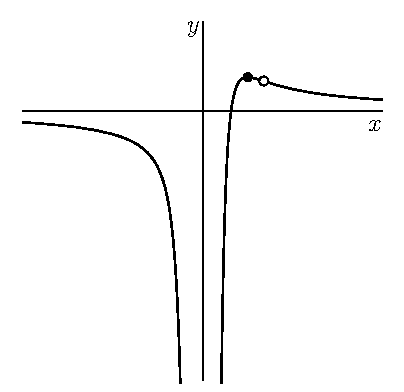
\includegraphics{graphE10b}
\begin{tikzpicture}
\YEaaxis{5}{5}{4}{1}
\draw[thick, red] plot[domain=-5:-1.15](\x,{2*(\x*\x*\x-2)/(\x*\x*\x*\x)});
\draw[thick, red] plot[domain=.9:5](\x,{2*(\x*\x*\x-2)/(\x*\x*\x*\x)});
\draw (2.7,0.65) node[opendot]{};
\draw (2,.75) node[vertex, label=above:{$\left(2,\frac{3}{8}\right)$}]{};
\YExcoord{2}{2}
\YExcoord{2.7}{\sqrt[3]{20}}
\YExcoord{1.3}{\sqrt[3]{2}}
\end{tikzpicture}
\end{center}
\end{answer}
\begin{hint}
The local maximum is also a global maximum.
\end{hint}
\begin{solution}
\begin{itemize}
\item Asymptotes:
\[\ds\lim_{x \to \pm \infty}f(x) = \ds\lim_{x \to \pm \infty}\dfrac{1}{x}-\dfrac{2}{x^4}=0\]
So $y=0$ is a horizontal asymptote both at $x=\infty$ and
$x=-\infty$.

\[\ds\lim_{x \to0}f(x) = \ds\lim_{x \to 0}\dfrac{x^3-2}{x^4}=-\infty\]
So there is a vertical asymptote at  $x=0$, where the function plunges downwards from both the right and the left.

\item Intervals of increase and decrease:

\[f'(x)=-\frac{1}{x^2}+\frac{8}{x^5}=\frac{8-x^3}{x^5}\]
The only place where $f'(x)$ is zero only at $x=2$. So $f(x)$ has a horizontal tangent at $x=2$,
$y=\frac{3}{8}$. This is a critical point.

The derivative is undefined at $x=0$, as is the function.

\begin{center}
 \begin{tabular}{|c||c|c|c|c|c|}
\hline
$x$  & $(-\infty,0)$ &$0$ & $(0,2)$ & $2$&$(2,\infty)$ \\
\hline
$f'(x)$  & negative  & DNE & positive & 0&  negative\\
\hline
$f(x)$ & decreasing & vertical asymptote & increasing &local max & decreasing\\
\hline
 \end{tabular}
\end{center}

Since the function changes from increasing to decreasing at $x=2$, the only local maximum is at $x=2$.

At this point, we get a rough sketch of $f(x)$.
\begin{center}
\begin{tikzpicture}
\YEaaxis{5}{5}{4}{1}
\draw[thick] (-4.5,-.25)--(-1,-.5)--(-.5,-4);
\draw[thick] (.5,-4)--(2,1)--(4.5,.25);
\YExcoord{2}{2}
\draw[thick, <-, orange] (-4,1)--(-2,2.5) ;
\draw[orange] (0,3)node{horizontal asymptotes $y=0$};
\draw[thick, <-, orange] (4,1)--(2,2.5);
\draw[blue, decorate, decoration={brace, amplitude=10pt, mirror}] (-5,-4.25)--(0,-4.25);
\draw[blue] (-2.5,-5)node{decreasing};
\draw[blue, decorate, decoration={brace, amplitude=10pt, mirror}] (2,-4.25)--(5,-4.25);
\draw[blue] (3.5,-5)node{decreasing};
\draw[red, decorate, decoration={brace, amplitude=10pt, mirror}] (0,-4.25)--(2,-4.25);
\draw[red] (1,-5)node{increasing};
\draw (2,1) node[vertex, label=above:{$\left(2,\frac{3}{8}\right)$}]{};
\end{tikzpicture}
\end{center}
%\item Global extrema:
%
%Since $\ds\lim_{x \to -\infty}f(x)=0$ and $f(x)$ is deceasing on $(-\infty, 0)$, we conclude $f(x)\le0$ for all $-\infty<x<0$.

\item Concavity:
\[f''(x)=\frac{2}{x^3}-\frac{40}{x^6}=\frac{2x^3-40}{x^6}\]
The second derivative of $f(x)$ is positive for $x>\root 3\of 20$ and negative for $x<\root 3\of 20$.
So the curve is concave up for $x>\root 3\of 20$ and concave down for
$x<\root 3\of 20$. There is an inflection point at $x=\root 3\of 20\approx 2.7$,
$y=\frac{18}{20^{4/3}}\approx 0.3$.

\item Intercepts:

Since $f(x)$ is not defined at $x=0$, there is no $y$-intercept. The only $x$-intercept is $x=\sqrt[3]{2}\approx 1.3$.

\item Sketch:


We can add concavity to our skeleton sketched above, and label our intercept and inflection point (the open dot).
\begin{center}
\begin{tikzpicture}
\YEaaxis{5}{5}{4}{1}
\draw[thick, red] plot[domain=-5:-1.15](\x,{2*(\x*\x*\x-2)/(\x*\x*\x*\x)});
\draw[thick, red] plot[domain=.9:5](\x,{2*(\x*\x*\x-2)/(\x*\x*\x*\x)});
\draw (2.7,0.65) node[opendot]{};
\draw (2,.75) node[vertex, label=above:{$\left(2,\frac{3}{8}\right)$}]{};
\YExcoord{2}{2}
\YExcoord{2.7}{\sqrt[3]{20}}
\YExcoord{1.3}{\sqrt[3]{2}}
\draw[blue, decorate, decoration={brace, amplitude=10pt, mirror}] (-5,-4.25)--(0,-4.25);
\draw[blue] (-2.5,-5)node{decreasing};
\draw[blue, decorate, decoration={brace, amplitude=10pt, mirror}] (2,-4.25)--(5,-4.25);
\draw[blue] (3.5,-5)node{decreasing};
\draw[red, decorate, decoration={brace, amplitude=10pt, mirror}] (0,-4.25)--(2,-4.25);
\draw[red] (1,-5)node{increasing};
\draw[blue, decorate, decoration={brace, amplitude=10pt, mirror}] (-5,-5.5)--(2.7,-5.5);
\draw[blue] (-1,-6.25)node{concave down};
\draw[red, decorate, decoration={brace, amplitude=10pt, mirror}] (2.7,-5.5)--(5,-5.5);
\draw[red] (4,-6.25)node{concave up};
\end{tikzpicture}
\end{center}
\end{itemize}
%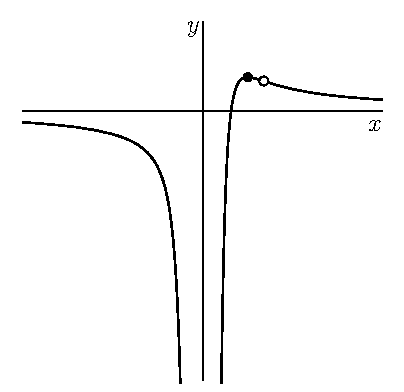
\includegraphics{graphE10b}
\end{solution}


\begin{question}[1997A]
The first and second derivatives of the function $f(x)=\dfrac{x^4}{1+x^3}$ are:
$$
f'(x)=\frac{4x^3+x^6}{(1+x^3)^2}\qquad\hbox{and}\qquad f''(x)=\frac{12x^2-6x^5}{(1+x^3)^3}
$$
Graph $f(x)$. Include local
and absolute maxima and minima, regions where $f(x)$ is increasing or
decreasing, regions where the curve is concave upward
or downward, and any asymptotes.
\end{question}
\begin{hint}
The sign of the first derivative is determined entirely by the numerator, but the sign of the second derivative depends on both the numerator and the denominator.
\end{hint}
\begin{answer}
The open dot marks the inflection point.
\begin{center}\begin{tikzpicture}
\YEaxis{6}{4}
\draw plot[domain=-3:-1.1, samples=50](2*\x,{\x*\x*\x*\x/(1+\x*\x*\x)});
\draw plot[domain=-0.93:3, samples=100](2*\x,{\x*\x*\x*\x/(1+\x*\x*\x)});
\draw[dashed](-2,-4)--(-2,-.75) (-2,.5)--(-2,4);
\YExcoord{-2}{-1}
\YExcoord{-3.2}{-\sqrt[3]{4}}
\YExcoord{2.52}{\sqrt[3]{2}}
\draw (2.53,0.84) node[opendot]{};
\draw (0,0) node[vertex]{};
\draw (-3.2,-2.12) node[vertex]{};
\end{tikzpicture}\end{center}
\end{answer}
\begin{solution}
\begin{itemize}
\item  Asymptotes:

When $x=-1$, the denominator $1+x^3$ of $f(x)$ is zero while the numerator is 1,  so $x=-1$ is a vertical asymptote. More precisely,
\[\lim_{x \to -1^-}f(x)=-\infty
\qquad
\lim_{x \to -1^+}f(x)=\infty\]

There are no horizontal asymptotes, because
\[\lim_{x \to \infty} \frac{x^4}{1+x^3}=\infty \qquad \lim_{x \to- \infty} \frac{x^4}{1+x^3}=-\infty\]

\item  Intervals of increase and decrease:

We note that $f'(x)$ is defined for all $x \neq -1$, so $f'(x)$ is defined for all $x$ in the domain of $f(x)$. Therefore, $f(x)$ has no singular points.

To find critical points, we set
\begin{align*}
f'(x)&=0\\
4x^3+x^6 &=0\\
x^3(4+x^3)&=0\\
x^3=0 \qquad &\mbox{or} \qquad 4+x^3=0\\
x=0 \qquad &\mbox{or} \qquad x=-\sqrt[3]{4}\approx-1.6
\end{align*}

At these critical points, $f(0)=0$ and
$f(-\root 3 \of 4)=\frac{4\root 3 \of 4}{-3}<0$.
The denominator of $f'(x)$ is never negative, so the sign of $f'(x)$ is the same as the sign of its numerator, $x^3(4+x^3)$.

\begin{center}
 \begin{tabular}{|c||c|c|c|c|c|c|c|}
\hline
$x$  & $(-\infty,-\sqrt[3]{4})$ &$-\sqrt[3]{4}$ & $(-\sqrt[3]{4},-1)$ & $-1$ &$(-1,0)$
&$0$&$(0,\infty)$\\
\hline
$f'(x)$  &  positive &0  &negative  &DNE &negative &0&positive \\
\hline
$f(x)$ & increasing & l. max&decreasing&VA &decreasing&l. min&increasing\\
\hline
 \end{tabular}
\end{center}

Now, we have enough information to make a skeleton of our graph.
\begin{center}\begin{tikzpicture}
\YEaxis{6}{4}
\YExcoord{-2}{-1}
\draw[dashed](-2,-4)--(-2,-.75) (-2,.5)--(-2,4);
\YExcoord{-3.2}{-\sqrt[3]{4}}
\draw[thick] (-6,-4)--(-3.2,-1)--(-2.3,-2)--(-2.1,-4);
\draw[thick] (-1.9,4)--(-1.7,2)--(0,0)--(6,4);
\draw[red, decorate, decoration={brace, amplitude=10pt, mirror}] (-6,-4.25)--(-3.2,-4.25);
\draw[red] (-4.8,-5)node{increasing};
\draw[blue, decorate, decoration={brace, amplitude=8pt, mirror}] (-3.2,-4.25)--(-2,-4.25);
\draw[blue] (-2.6,-5)node{decr};
\draw[blue, decorate, decoration={brace, amplitude=10pt, mirror}] (-2,-4.25)--(0,-4.25);
\draw[blue] (-1,-5)node{decr};
\draw[red, decorate, decoration={brace, amplitude=10pt, mirror}] (0,-4.25)--(6,-4.25);
\draw[red] (3,-5)node{increasing};
\end{tikzpicture}\end{center}

\item Concavity:

The second derivative is undefined when $x=-1$. It is zero when $12x^2-6x^5=6x^2(2-x^3)=0$.
That is, at $x=\root 3\of 2\approx 1.3$ and $x=0$.  Notice that the sign of $f''(x)$ does not change at $x=0$, so $x=0$ is not an inflection point.


\begin{center}
 \begin{tabular}{|c||c|c|c|c|c|c|c|}
\hline
$x$  & $(-\infty,-1)$ &$-1$ & $(-1,0)$ & $0$ &$(0,\sqrt[3]{2})$
&$\sqrt[3]{2}$&$(\sqrt[3]{2},\infty)$\\
\hline
$f''(x)$  &  negative &DNE  &positive  &0 &positive &0&negative \\
\hline
$f(x)$ & concave down & VA&concave up&&concave up&IP&concave down\\
\hline
 \end{tabular}
\end{center}

Now we can refine our skeleton by adding concavity.
\begin{center}\begin{tikzpicture}
\YEaxis{6}{4}
\draw plot[domain=-3:-1.1, samples=50](2*\x,{\x*\x*\x*\x/(1+\x*\x*\x)});
\draw plot[domain=-0.93:3, samples=100](2*\x,{\x*\x*\x*\x/(1+\x*\x*\x)});
\draw[dashed](-2,-4)--(-2,-.75) (-2,.5)--(-2,4);
\YExcoord{-2}{-1}
\YExcoord{-3.2}{-\sqrt[3]{4}}
\YExcoord{2.52}{\sqrt[3]{2}}
\draw[red, decorate, decoration={brace, amplitude=10pt, mirror}] (-6,-4.25)--(-3.2,-4.25);
\draw[red] (-4.8,-5)node{increasing};
\draw[blue, decorate, decoration={brace, amplitude=8pt, mirror}] (-3.2,-4.25)--(-2,-4.25);
\draw[blue] (-2.8,-5)node{decr};
\draw[blue, decorate, decoration={brace, amplitude=10pt, mirror}] (-2,-4.25)--(0,-4.25);
\draw[blue] (-1,-5)node{decr};
\draw[red, decorate, decoration={brace, amplitude=10pt, mirror}] (0,-4.25)--(6,-4.25);
\draw[red] (3,-5)node{increasing};
\draw[blue, decorate, decoration={brace, amplitude=10pt, mirror}] (-6,-5.5)--(-2,-5.5);
\draw[blue] (-4,-6.25)node{concave down};
\draw[red, decorate, decoration={brace, amplitude=10pt, mirror}] (-2,-5.5)--(2.5,-5.5);
\draw[red] (0.25,-6.25)node{concave up};
\draw[blue, decorate, decoration={brace, amplitude=10pt, mirror}] (2.5,-5.5)--(6,-5.5);
\draw[blue] (4.25,-6.25)node{concave down};

\draw (2.53,0.84) node[opendot]{};
\draw (0,0) node[vertex]{};
\draw (-3.2,-2.12) node[vertex]{};
\end{tikzpicture}\end{center}
\end{itemize}
%\begin{center}
%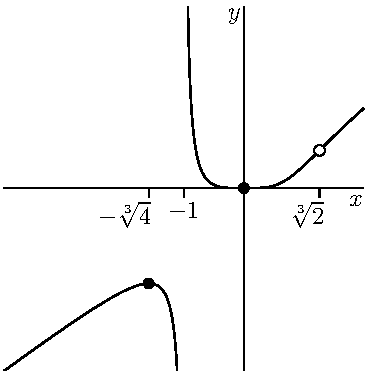
\includegraphics{graphW58}\end{center}
\end{solution}


\begin{Mquestion}[1996D]\label{s3.6.6rationallast}
 The first and second derivatives of the function $f(x)=\dfrac{x^3}{1-x^2}$ are:
$$
f'(x)=\frac{3x^2-x^4}{(1-x^2)^2}\qquad\hbox{and}\qquad f''(x)=\frac{6x+2x^3}{(1-x^2)^3}
$$
Graph $f(x)$. Include local
and absolute maxima and minima, regions where the curve is concave upward
or downward, and any asymptotes.
\end{Mquestion}
\begin{hint}
The function is odd.
\end{hint}
\begin{answer}
\begin{center}
%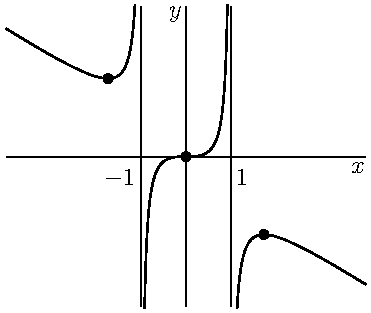
\includegraphics{graphE5}
\begin{tikzpicture}
\YEaxis{6}{4}
\draw plot[domain=-3:-1.08, samples=50](2*\x,{\x*\x*\x/(1-\x*\x)/2});
\draw plot[domain=-.945:.945, samples=50](2*\x,{\x*\x*\x/(1-\x*\x)/2});
\draw plot[domain=1.08:3, samples=50](2*\x,{\x*\x*\x/(1-\x*\x)/2});
\YExcoord{-2}{-1}
\YExcoord{2}{1}
\YExcoord{-3.46}{-\sqrt{3}}
\YExcoord{3.46}{\sqrt{3}}
\YEycoord{1.3}{\frac{3\sqrt{3}}{2}}
\YEycoord{-1.3}{-\frac{3\sqrt{3}}{2}}
\draw[dashed] (-2,-4)--(-2,-1) (-2,.5)--(-2,4);
\draw[dashed] (2,-4)--(2,-1) (2,.5)--(2,4);
\draw(-3.46,1.3) node[vertex]{};
\draw(3.46,-1.3) node[vertex]{};
\draw(0,0) node[opendot]{};
\end{tikzpicture}
\end{center}
\end{answer}
\begin{solution}
\begin{itemize}
\item Asymptotes:
\[\lim_{x \to -\infty}\frac{x^3}{1-x^2}=\infty \qquad
\lim_{x \to \infty}\frac{x^3}{1-x^2}=-\infty \]
So, $f(x)$ has no horizontal asymptotes.

 On the other hand $f(x)$ blows up at both $x=1$
and $x=-1$, so there are vertical asymptotes at $x=1$ and $x=-1$.
More precisely,
\begin{align*}
\lim_{x \to -1^-}\frac{x^3}{1-x^2}&=\infty
&
\lim_{x \to -1^+}\frac{x^3}{1-x^2}&=-\infty\\
\lim_{x \to 1^-}\frac{x^3}{1-x^2}&=\infty
&
\lim_{x \to 1^+}\frac{x^3}{1-x^2}&=-\infty
\end{align*}

\item Symmetry:

$f(x)$ is an odd function, because
\[f(-x)=\frac{(-x)^3}{1-(-x)^2}=\frac{-x^3}{1-x^2}=-f(x)\]

\item Intercepts:

The only intercept of $f(x)$ is the origin. In particular, that means that out of the three intervals where it is continuous,
                  namely $(-\infty,-1)$, $(-1,1)$ and $(1,\infty)$, in two of them $f(x)$ is always positive or always negative.
\begin{itemize}
\item When $x<-1$:\quad $1-x^2<0$ and $x^3<0$, so $f(x)>0$.
\item When $x>1$:\qquad $1-x^2<0$ and $x^3>0$, so $f(x)<0$.
\item When $-1<x<0$, $1-x^2>0$ and $x^3<0$ so $f(x)<0$.
\item When $0<x<1$, $1-x^2>0$ and $x^3>0$ so $f(x)>0$.
\end{itemize}

\item Intervals of increase and decrease:

\[f'(x)=\dfrac{3x^2-x^4}{(1-x^2)^2}=\frac{x^2(3-x^2)}{(1-x^2)^2}\]
There are no singular points (but remember the domain of $f(x)$ does not include $x=\pm 1$ ). The critical points are:
\begin{align*}
f'(x)&=0\\
x^2=0\qquad&\mbox{or}\qquad 3-x^2=0\\
x=0\qquad&\mbox{or}\qquad x=\pm\sqrt{3}\approx\pm 1.7
\end{align*}

The values of $f$ at its critical points are
$f(0)=0$, $f(\sqrt{3})=-\dfrac{3\sqrt{3}}{2}\approx -2.6$ and $f(-\sqrt{3})=\dfrac{3\sqrt{3}}{2}\approx2.6$.

Notice the sign of $f'(x)$ is the same as the sign of $3-x^2$.

\begin{center}
 \begin{tabular}{|c||c|c|c|c|c|c|c|}
\hline
$x$  & $(-\infty,-\sqrt{3})$ &$-\sqrt{3}$&$(-\sqrt 3,-1)$&$-1$\\
\hline
$f'(x)$  &negative&0&positive&DNE\\
\hline
$f(x)$ & decreasing&local min&increasing&VA\\
\hline
 \end{tabular}

 \begin{tabular}{|c||c|c|c|c|c|c|c|}
\hline
$x$  & $(-1,0)$ &$0$&$(0,\sqrt 3)$&$\sqrt{3}$&$(\sqrt{3},\infty)$\\
\hline
$f'(x)$  &positive&0&positive&0&negative\\
\hline
$f(x)$ &increasing & & increasing & local max & decreasing \\
\hline
 \end{tabular}
\end{center}

Now we have enough information to sketch a skeleton of $f(x)$.

\begin{center}
\begin{tikzpicture}
\YEaxis{6}{4}
\YExcoord{-2}{-1}
\YExcoord{2}{1}
\YExcoord{-3.46}{-\sqrt{3}}
\YExcoord{3.46}{\sqrt{3}}
\YEycoord{1.3}{\frac{3\sqrt{3}}{2}}
\YEycoord{-1.3}{-\frac{3\sqrt{3}}{2}}
\draw[dashed] (-2,-4)--(-2,-1) (-2,.5)--(-2,4);
\draw[dashed] (2,-4)--(2,-1) (2,.5)--(2,4);
\draw[blue, decorate, decoration={brace, amplitude=10pt, mirror}] (-6,-4.25)--(-3.46,-4.25);
\draw[blue] (-4.75,-5) node{decreasing};
\draw[red, decorate, decoration={brace, amplitude=10pt, mirror}] (-3.46,-4.25)--(-2,-4.25);
\draw[red] (-2.75,-5) node{incr};
\draw[red, decorate, decoration={brace, amplitude=10pt, mirror}] (-2,-4.25)--(2,-4.25);
\draw[red] (0,-5) node{increasing};
\draw[red, decorate, decoration={brace, amplitude=10pt, mirror}] (2,-4.25)--(3.46,-4.25);
\draw[red] (2.75,-5) node{incr};
\draw[blue, decorate, decoration={brace, amplitude=10pt, mirror}] (3.46,-4.25)--(6,-4.25);
\draw[blue] (4.75,-5) node{decreasing};
\draw(-3.46,1.3) node[vertex]{};
\draw(3.46,-1.3) node[vertex]{};
\draw(0,0) node[vertex]{};
\draw[thick] (-6,4)--(-3.46,1.3)--(-2.2,2)--(-2.1,4);
\draw[thick] (6,-4)--(3.46,-1.3)--(2.2,-2)--(2.1,-4);
\draw[thick] (-1.9,-4)--(-1.8,-1)--(-.5,0)--(.5,0)--(1.8,2)--(1.9,4);
\end{tikzpicture}
\end{center}

\item Concavity:
\[f''(x)=\frac{2x(3+x^2)}{(1-x^2)^3}\]

The second derivative is zero when $x=0$, and is undefined when $x=\pm 1$.

\begin{center}
 \begin{tabular}{|c||c|c|c|c|c|c|c|}
\hline
$x$  & $(-\infty,-1)$ &$(-1,0)$&0&$(0,1)$&$(1,\infty)$\\
\hline
$f''(x)$  &positive&negative&0&positive&negative\\
\hline
$f(x)$ & concave up&concave down&inflection point&concave up&concave down\\
\hline
 \end{tabular}
\end{center}
Now, we can refine our skeleton.

\begin{center}
\begin{tikzpicture}
\YEaxis{6}{4}
\draw plot[domain=-3:-1.08, samples=50](2*\x,{\x*\x*\x/(1-\x*\x)/2});
\draw plot[domain=-.945:.945, samples=50](2*\x,{\x*\x*\x/(1-\x*\x)/2});
\draw plot[domain=1.08:3, samples=50](2*\x,{\x*\x*\x/(1-\x*\x)/2});
\YExcoord{-2}{-1}
\YExcoord{2}{1}
\YExcoord{-3.46}{-\sqrt{3}}
\YExcoord{3.46}{\sqrt{3}}
\YEycoord{1.3}{\frac{3\sqrt{3}}{2}}
\YEycoord{-1.3}{-\frac{3\sqrt{3}}{2}}
\draw[dashed] (-2,-4)--(-2,-1) (-2,.5)--(-2,4);
\draw[dashed] (2,-4)--(2,-1) (2,.5)--(2,4);
\draw(-3.46,1.3) node[vertex]{};
\draw(3.46,-1.3) node[vertex]{};
\draw(0,0) node[opendot]{};

\draw[blue, decorate, decoration={brace, amplitude=10pt, mirror}] (-6,-4.25)--(-3.46,-4.25);
\draw[blue] (-4.75,-5) node{decreasing};
\draw[red, decorate, decoration={brace, amplitude=10pt, mirror}] (-3.46,-4.25)--(-2,-4.25);
\draw[red] (-2.75,-5) node{incr};
\draw[red, decorate, decoration={brace, amplitude=10pt, mirror}] (-2,-4.25)--(2,-4.25);
\draw[red] (0,-5) node{increasing};
\draw[red, decorate, decoration={brace, amplitude=10pt, mirror}] (2,-4.25)--(3.46,-4.25);
\draw[red] (2.75,-5) node{incr};
\draw[blue, decorate, decoration={brace, amplitude=10pt, mirror}] (3.46,-4.25)--(6,-4.25);
\draw[blue] (4.75,-5) node{decreasing};
\draw[red, decorate, decoration={brace, amplitude=10pt, mirror}] (-6,-5.5)--(-2,-5.5);
\draw[red] (-4,-6.25) node{concave up};
\draw[blue, decorate, decoration={brace, amplitude=10pt, mirror}] (-2,-5.5)--(0,-5.5);
\draw[blue] (-1,-6.25) node{cc down};
\draw[red, decorate, decoration={brace, amplitude=10pt, mirror}] (0,-5.5)--(2,-5.5);
\draw[red] (1,-6.25) node{concave up};
\draw[blue, decorate, decoration={brace, amplitude=10pt, mirror}] (2,-5.5)--(6,-5.5);
\draw[blue] (4,-6.25) node{concave down};
\end{tikzpicture}
\end{center}
%\begin{center}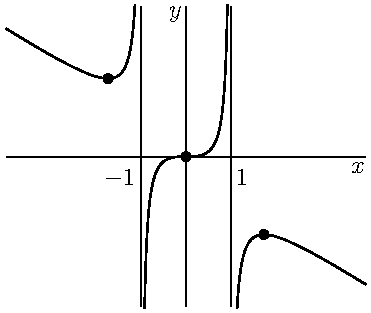
\includegraphics{graphE5}\end{center}
\end{itemize}
\end{solution}






\begin{Mquestion}[2006H]
The function $f(x)$ is defined by
\[
f(x) =
\left\{\begin{array}{lc}
e^x &x<0\\
 \frac{x^2+3}{3(x+1)} & x \ge 0
 \end{array}\right.
\]
\begin{enumerate}[(a)]
\item\label{s3.6_2006_a} Explain why $f(x)$ is continuous everywhere.
\item\label{s3.6_2006_b} Determine all of the following if they are present:

\begin{enumerate}[i.]
\item\label{s3.6_2006_i} $x$--coordinates of local maxima and minima, intervals
          where $f(x)$ is increasing or decreasing;
\item\label{s3.6_2006_ii} intervals where $f(x)$ is concave upwards or downwards;
\item\label{s3.6_2006_iii} equations of any horizontal or vertical asymptotes.
\end{enumerate}

\item\label{s3.6_2006_c} Sketch the graph of $y = f(x)$, giving the $(x, y)$
coordinates for all points of interest above.
\end{enumerate}
\end{Mquestion}
\begin{hint}
The function is continuous at $x=0$, but its derivative is not.
\end{hint}
\begin{answer}
\eqref{s3.6_2006_a}
One branch of the function,
the exponential function $e^x$, is continuous everywhere. So $f(x)$ is continuous for $x<0$. When $x \geq 0$, $f(x)=\dfrac{x^2+3}{3(x+1)}$, which is continuous whenever $x \neq -1$ (so it's continuous for all $x >0$). So, $f(x)$ is continuous for $x>0$. To see that $f(x)$ is continuous at $x=0$, we see:
\begin{align*}
\lim_{x\rightarrow0-}f(x)=\lim_{x\rightarrow0-}e^x&=1\\
\lim_{x\rightarrow0+}f(x)=\lim_{x\rightarrow0+}\frac{x^2+3}{3(x+1)}&=1\\
\mbox{So, }~\lim_{x \rightarrow 0}f(x)&=1=f(0)
\end{align*}
Hence $f(x)$ is continuous at $x=0$, so $f(x)$ is continuous everywhere.\\
\eqref{s3.6_2006_b}
i.\\  $f(x)$ is increasing for $x<0$ and $x>1$, decreasing for $0<x<1$,
            has a local max at $(0,1)$, and has a local min at $\left(1,\frac{2}{3}\right)$.\\
ii.\\ $f(x)$ is concave upwards for all $x\ne 0$.\\
iii.\\ The $x$--axis is a horizontal asymptote as $x\rightarrow-\infty$.

\eqref{s3.6_2006_c}
%\centerline{\figput{OE06D_3}}
\begin{center}\begin{tikzpicture}
\YEaaxis{3}{3}{.5}{2}
\draw[thick] plot[domain=-3:0](\x,{exp(\x)});
\draw (0,1) node[vertex, label=above left:{$(0,1)$}]{};
\draw[thick] plot[domain=0:3](\x,{(\x*\x+3)/(3*\x+3)});
\draw (1,2/3) node[vertex, label=above:{$(1,\frac{2}{3})$}]{};
\end{tikzpicture}\end{center}
\end{answer}
\begin{solution}
\eqref{s3.6_2006_a}
One branch of the function,
the exponential function $e^x$, is continuous everywhere. So $f(x)$ is continuous for $x<0$. When $x \geq 0$, $f(x)=\dfrac{x^2+3}{3(x+1)}$, which is continuous whenever $x \neq -1$ (so it's continuous for all $x >0$). So, $f(x)$ is continuous for $x>0$. To see that $f(x)$ is continuous at $x=0$, we see:
\begin{align*}
\lim_{x\rightarrow0-}f(x)=\lim_{x\rightarrow0-}e^x&=1\\
\lim_{x\rightarrow0+}f(x)=\lim_{x\rightarrow0+}\frac{x^2+3}{3(x+1)}&=1\\
\mbox{So, }~\lim_{x \rightarrow 0}f(x)&=1=f(0)
\end{align*}
Hence $f(x)$ is continuous at $x=0$, so $f(x)$ is continuous everywhere.\\
\eqref{s3.6_2006_b}
We differentiate the function twice.
 Notice
 \begin{align*}
 \diff{}{x}\left\{\dfrac{x^2+3}{3(x+1)}\right\}&=\frac{3(x+1)(2x)-(x^2+3)(3)}{9(x+1)^2}\\
&=\frac{x^2+2x-3}{3(x+1)^2}\\
 &=\frac{(x-1)(x+3)}{3(x+1)^2}\qquad\mbox{where $x \neq -1$}\\
 \mbox{Then}\qquad
  \lim_{x \to 0^+}f'(x)&=\frac{(0-1)(0+3)}{3(0+1)^2}=-1 \neq 1 =e^0= \lim_{x \to 0^-}f'(x)\\
 \mbox{so}\qquad
f'(x)&=\left\{\begin{array}{ll}
e^x&x<0\\
DNE&x=0\\
\frac{(x-1)(x+3)}{3(x+1)^2}&x > 0
\end{array}\right.\\
 \intertext{Differentiating again,}
 \diff{^2}{x^2}\left\{\dfrac{x^2+3}{3(x+1)}\right\}&=
 \diff{}{x}\left\{\frac{x^2+2x-3}{3(x+1)^2}
 \right\}\\
 &=\frac{3(x+1)^2(2x+2)-(x^2+2x-3)(6)(x+1)}{9(x+1)^4}\left(\frac{\div3(x+1)}{\div3(x+1)}\right)\\
 &=\frac{(x+1)(2x+2)-2(x^2+2x-3)}{3(x+1)^3}\\
 &=\frac{8}{3(x+1)^3}\qquad\mbox{where $x \neq -1$}\\
 \mbox{so}\qquad
f''(x)&=\left\{\begin{array}{ll}
e^x&x<0\\
DNE&x=0\\
\frac{8}{3(x+1)^3}&x > 0
\end{array}\right.
 \end{align*}

i.
The only singular point is $x=0$, and the only critical point is $x=1$. (When you're reading off the expression for $f'(x)$, remember that the bottom line only applies when $x>0$.)
\begin{center}
\begin{tabular}{|c||c|c|c|c|c|}
\hline
$x$&$(-\infty,0)$&$0$&$(0,1)$&1&$(1,\infty)$\\
\hline
$f'(x)$&positive&DNE&negative&0&positive\\
\hline
$f(x)$&increasing&local max&decreasing&local min&increasing\\
\hline
\end{tabular}
\end{center}
The coordinates of the local maximum are $(0,1)$
and the coordinates of the local minimum are $\left(1,\frac{2}{3}\right)$.

ii.\\  When $x \neq 0$, $f''(x)$ is always positive, so $f(x)$ is concave up.\\
iii.\\
\begin{align*}
\lim_{x \to \infty} f(x)&=\lim_{x \to \infty} \frac{x^2+3}{3x+3}\\
&=\lim_{x \to \infty}\frac{x+\frac{3}{x}}{1+\frac{3}{x}}=\infty
\intertext{So, there is no horizontal asymptote to the right.}
\lim_{x \to -\infty} f(x)&=\lim_{x \to -\infty}e^x=0
\intertext{So, $y=0$ is a horizontal asymptote to the left.}
\end{align*}
Since $f(x)$ is continuous everywhere, there are no vertical asymptotes.

\eqref{s3.6_2006_c}
%\centerline{\figput{OE06D_3}}
\begin{center}\begin{tikzpicture}
\YEaaxis{3}{3}{.5}{2}
\draw[thick] plot[domain=-3:0](\x,{exp(\x)});
\draw (0,1) node[vertex, label=above left:{$(0,1)$}]{};
\draw[thick] plot[domain=0:3](\x,{(\x*\x+3)/(3*\x+3)});
\draw (1,2/3) node[vertex, label=above:{$(1,\frac{2}{3})$}]{};
\draw[red, decorate, decoration={brace, amplitude=10pt, mirror}](-3,-.75)--(0,-.75);
\draw[red] (-1.5,-1.5) node{increasing};
\draw[blue, decorate, decoration={brace, amplitude=6pt, mirror}](0,-.75)--(1,-.75);
\draw[blue] (.5,-1.5) node{decr};
\draw[red, decorate, decoration={brace, amplitude=10pt, mirror}](1,-.75)--(3,-.75);
\draw[red] (2,-1.5) node{increasing};
\draw[red, decorate, decoration={brace, amplitude=10pt, mirror}](-3,-2)--(0,-2);
\draw[red] (-1.5,-2.75) node{concave up};
\draw[red, decorate, decoration={brace, amplitude=10pt, mirror}](0,-2)--(3,-2);
\draw[red] (1.5,-2.75) node{concave up};
\end{tikzpicture}\end{center}
\end{solution}


\Instructions{In Questions~\ref{s3.6.6expfirst} and \ref{s3.6.6explast}, you will sketch the graphs of functions with an exponential component. In the next section, you will learn how to find their horizontal asymptotes, but for now these are given to you.}

\begin{question}[1997D]\label{s3.6.6expfirst}
The function $f(x)$ and its derivative are given below:
\[
f(x)=(1+2x)e^{-x^2}\qquad\hbox{and}\qquad f'(x)=2(1-x-2x^2)e^{-x^2}
\]
Sketch the graph of $f(x)$. Indicate the critical points, local
and/or absolute maxima and minima, and asymptotes. Without actually calculating
the inflection points, indicate on the graph their approximate location.

Note: $\ds\lim_{x \to \pm\infty}f(x)=0$.
\end{question}
\begin{hint}
Since you aren't asked to find the intervals of concavity exactly, sketch the intervals of increase and decrease, and turn them into a smooth curve. You might not get exactly the intervals of concavity that are given in the solution, but there should be the same number of intervals as the solution, and they should have the same positions relative to the local extrema.
\end{hint}
\begin{answer}\begin{center}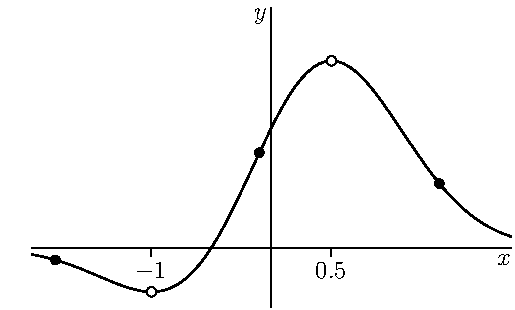
\includegraphics{graphE12}\end{center}
\end{answer}
\begin{solution}
\begin{itemize}
\item Asymptotes:
In the problem statement, we are told:
\[\lim_{x \to \pm \infty}\frac{1+2x}{e^{x^2}}=0\]
So, $y=0$ is a horizontal asymptote both at $x=\infty$ and at $x=-\infty$.

Since $f(x)$ is continuous, it has no vertical asymptotes.

\item Intervals of increase and decrease:

The critical points are the zeroes of $1-x-2x^2=(1-2x)(1+x)$. That is,
 $x=\frac{1}{2},\ -1$.

\begin{center}
\begin{tabular}{|c||c|c|c|c|c|}
\hline
$x$&$(-\infty,-1)$&$-1$&$(-1,\frac{1}{2})$&$\frac{1}{2}$&$(\frac{1}{2},\infty)$\\
\hline
$f'(x)$&negative&0&positive&0&negative\\
\hline
$f(x)$&decreasing&local min&increasing&local max&decreasing\\
\hline
\end{tabular}
\end{center}
At these critical points, $f\big(\frac{1}{2}\big)=2e^{-1/4}>0$ and $f(-1)=-e^{-1}<0$.

From here, we can sketch a skeleton of the graph.
\begin{center}
\begin{tikzpicture}
\YEaaxis{4.25}{4.25}{1}{3}
\YExcoord{-2}{-1}
\YExcoord{1}{\frac{1}{2}}
\draw[thick] (-4,-.1)--(-2,-.3)--(1,2)--(2,.5)--(4,.25);
\draw[blue, decorate, decoration={brace, amplitude=10pt, mirror}] (-4,-1)--(-2,-1);
\draw[blue] (-3,-1.75) node{decreasing};
\draw[red, decorate, decoration={brace, amplitude=10pt, mirror}] (-2,-1)--(1,-1);
\draw[red] (-.5,-1.75) node{increasing};
\draw[blue, decorate, decoration={brace, amplitude=6pt, mirror}] (1,-1)--(2,-1);
\draw[blue] (1.5,-1.75) node{decr};
\draw[red, decorate, decoration={brace, amplitude=10pt, mirror}] (2,-1)--(4,-1);
\draw[red] (3,-1.75) node{increasing};
%\draw[thick] plot[domain=-2:2](2*\x,{(1+2*\x)/(exp(\x*\x))});
\end{tikzpicture}
\end{center}

\item Concavity:

We are told that we don't have to actually solve for the inflection points. We just need to know enough to get a basic idea. So, we'll turn the skeleton of the graph into smooth curve.

\begin{center}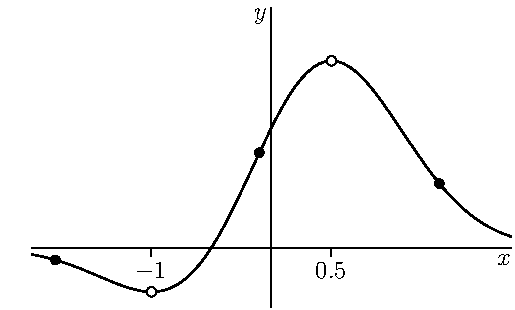
\includegraphics{graphE12}\end{center}

Inflection points are points where the convexity changes from up
to down or vice versa. It looks like our graph is convex down for $x$ from
$-\infty$ to about $-1.8$, convex up from about $x=-1.8$ to about $x=-0.1$,
convex down from about $x=-0.1$ to about $x=1.4$ and convex up from about
$x=1.4$ to infinity. So there are three inflection points at roughly
$x=-1.8,\ -0.1,\ 1.4$.
\end{itemize}
\end{solution}


\begin{Mquestion}[2009H]\label{s3.6.6explast}
Consider the function $f(x) = xe^{-x^2/2}$.

Note: $\ds\lim_{x \to \pm\infty}f(x)=0$.
\begin{enumerate}[(a)]
%\item\label{s3.62009_1} Find $\ds\lim_{x \to \infty}f(x)$ and $\ds\lim_{x \to -\infty}f(x)$.
\item\label{s3.62009_2} Find all inflection points and intervals of increase, decrease,
 convexity up, and convexity down. \\You may use without proof the formula
$f''(x) = (x^3-3x)e^{-x^2/2}$.
\item\label{s3.62009_3} Find local and global minima and maxima.
\item\label{s3.62009_4}  Use all the above to draw a graph for $f$. Indicate all
special points on the graph.
\end{enumerate}
\end{Mquestion}
\begin{hint}
Use intervals of increase and decrease, concavity, and asymptotes to sketch the curve.
\end{hint}
\begin{answer}
\eqref{s3.62009_2}
Increasing: $(-1,1)$\qquad decreasing: $(-\infty,-1)\cup (1,\infty)$\\
concave up: $(-\sqrt{3},0) \cup (\sqrt{3},\infty)$\qquad concave down: $(-\infty,-\sqrt{3}) \cup (0 ,\sqrt{3})$\\
inflection points: $x=\pm\sqrt{3}, 0$

\eqref{s3.62009_3}
The local and global minimum of $f(x)$ is at $(-1,\frac{-1}{\sqrt{e}})$, and the local and global maximum of $f(x)$ is at $(1,\frac{1}{\sqrt{e}})$.

\eqref{s3.62009_4}
In the graph below, open dots are inflection points, and
solid dots are extrema.
\begin{center}\begin{tikzpicture}
\YEaxis{6.5}{3};
\draw[thick] plot[domain=-3:3, scale=2, samples=100](\x,{2*\x*exp(-\x*\x/2)});
\draw (3.5,1.54) node[opendot]{};
\draw (-3.5,-1.53) node[opendot]{};
\YExcoord{-2}{-1}
\YExcoord{2}{1}
\draw (-3.5,.2) -- (-3.5,-.05) node[below]{$-\sqrt{3}$};
\YExcoord{3.5}{\sqrt{3}}
\YEycoord{-2.4}{\dfrac{-1}{\sqrt e}}
\YEycoord{2.4}{\dfrac{1}{\sqrt e}}
\draw (2,2.4) node[vertex]{};
\draw (-2,-2.4) node[vertex]{};
\end{tikzpicture}\end{center}
\end{answer}
\begin{solution}

\eqref{s3.62009_2}  We need to know the first and second derivative of $f(x)$. Using the product and chain rules, $f'(x)=e^{-x^2/2}(1-x^2)$. Given to us is $f''(x) = (x^3-3x)e^{-x^2/2}$. (These derivatives are also easy to find using the formula developed in Question~\ref{s2.14expprod}, Section~\ref*{sec higher diff}.)%2.14, higher order derivatives

Since $e^{-x^2/2}$ is always positive, the sign of $f'(x)$ is the same as the sign of $1-x^2$. $f(x)$ has no singular points and its only critical points are $x=\pm 1$. At these critical points, $f(-1)=-\dfrac{1}{\sqrt{e}}$ and $f(1)=\dfrac{1}{\sqrt{e}}$.
\begin{center}
\begin{tabular}{|c||c|c|c|c|c|}
\hline
$x$&$(-\infty,-1)$&$-1$&$(-1,1)$&$1$&$(1,\infty)$\\
\hline
$f'(x)$&negative&0&positive&0&negative\\
\hline
$f(x)$&decreasing&local min&increasing&local max&decreasing\\
\hline
\end{tabular}
\end{center}

This, together with the observations that $f(x)<0$ for $x<0$,
          $f(0)=0$ and $f(x)>0$ for $x>0$ (in fact $f$ is an odd function),
          is enough to sketch a skeleton of our graph.

\begin{center}\begin{tikzpicture}
\YEaxis{5}{2};
\draw (-2,.2) -- (-2,-.2) node[below]{$-1$};
\draw (2,.2) -- (2,-.2) node[below]{$1$};
\draw (.2,-1)--(-.2,-1) node[left]{$-\frac{1}{\sqrt{e}}$};
\draw (.2,1)--(-.2,1) node[left]{$\frac{1}{\sqrt{e}}$};
\draw[ thick] (-5,-.1)-- (-4,-.2)--(-2,-1);
\draw[thick] (-2,-1)--(2,1);
\draw[thick] (2,1)--(4,.2)--(5,.1);
\end{tikzpicture}\end{center}


We can factor $f''(x) = (x^3-3x)e^{-x^2/2}=x(x+\sqrt{3})(x-\sqrt{3})e^{-x^2/2}$. Since $e^{-x^2/2}$ is always positive, the sign of $f''(x)$ is the same as the sign of $x(x+\sqrt{3})(x-\sqrt{3})$.

\begin{center}
\begin{tabular}{|c||c|c|c|c|c|c|c|}
\hline
$x$&$(-\infty,-\sqrt{3})$&$-\sqrt{3}$&$(-\sqrt{3},0)$
&0&$(0,\sqrt{3})$
&$\sqrt{3}$&$(\sqrt{3},\infty)$\\
\hline
$f''(x)$&negative&0&positive&0&negative&0&positive\\
\hline
$f(x)$&concave down&IP&concave up&IP&concave down&IP&concave up\\
\hline
\end{tabular}
\end{center}

\eqref{s3.62009_3} We've already seen that $f(x)$ has a local min at $x=-1$ and a local max at $x=1$.

As $x$ tends to negative infinity, $f(x)$ tends to 0, and $f(x)$ is decreasing on $(-\infty,-1)$. Then $f(x)$ is between $0$ and $f(-1)=\frac{-1}{\sqrt{e}}$ on $(-\infty,-1)$. Then $f(x)$ is increasing on $(-1,1)$ from $f(-1)=\frac{-1}{\sqrt{e}}$ to $f(1)=\frac{1}{\sqrt{e}}$. Finally, for $x>1$, $f(x)$ is decreasing from $f(1)=\frac{1}{\sqrt{e}}$ and tending to 0. So when $x>1$, $f(x)$ is between $\frac{1}{\sqrt{e}}$ and $0$.

So, over its entire domain, $f(x)$ is between $\frac{-1}{\sqrt{e}}$ and $\frac{1}{\sqrt{e}}$, and it only achieves those values at $x=-1$ and $x=1$, respectively. Therefore, the local and global min of $f(x)$ is at $(-1,\frac{-1}{\sqrt{e}})$, and the local and global max of $f(x)$ is at $(1,\frac{1}{\sqrt{e}})$.

\eqref{s3.62009_4}
In the graph below, open dots are inflection points, and
solid dots are extrema.
\begin{center}\begin{tikzpicture}
\YEaxis{6.5}{3};
\draw[thick] plot[domain=-3:3, scale=2, samples=100](\x,{2*\x*exp(-\x*\x/2)});
\draw (3.5,1.54) node[opendot]{};
\draw (-3.5,-1.53) node[opendot]{};
\YExcoord{-2}{-1}
\YExcoord{2}{1}
\draw (-3.5,.2) -- (-3.5,-.05) node[below]{$-\sqrt{3}$};
\YExcoord{3.5}{\sqrt{3}}
\YEycoord{-2.4}{\dfrac{-1}{\sqrt e}}
\YEycoord{2.4}{\dfrac{1}{\sqrt e}}
\draw (2,2.4) node[vertex]{};
\draw (-2,-2.4) node[vertex]{};
\end{tikzpicture}\end{center}
%\centerline{\figput{OE09D_4}}
\end{solution}

\Instructions{In Questions~\ref{s3.6.6trig1} and \ref{s3.6.6trig2}, you will sketch the graphs of functions that have a trigonometric component.}

\begin{question}\label{s3.6.6trig1}
Use the techniques from this section to sketch the graph of $f(x)=x+2\sin x$.
\end{question}
\begin{hint}
Although the function exhibits a certain kind of repeating behaviour, it is not periodic.
\end{hint}
\begin{answer}
Local maxima occur at $x=\frac{2\pi}{3}+2\pi n$ for all integers $n$, and local minima occur at $x=-\frac{2\pi}{3}+2\pi n$ for all integers $n$. Inflection points occur at
every integer multiple of $\pi$.
\begin{center}
\begin{tikzpicture}
\YEaxis{5.5}{5.5};
\draw[thick] plot[domain=-15:15, samples=100](\x/3,{(\x+2*sin(\x r))/3});
\foreach \x in {2,4,8,10,14}
	{\YExcoord{\x*3.14/9}{\frac{\x \pi}{3}}
	\YExcoord{-\x*3.14/9}{\frac{-\x \pi}{3}}
	}
\end{tikzpicture}
\end{center}
\end{answer}
\begin{solution}
\begin{itemize}
\item Symmetry:

\[f(-x)=-x+2\sin(-x)=-x-2\sin x = -f(x)\]
So, $f(x)$ is an odd function. If we can sketch $y=f(x)$ for nonnegative $x$, we can use symmetry to complete the curve for all $x$.
\item Asymptotes:

Since $f(x)$ is continuous, it has no vertical asymptotes. It also has no horizontal asymptotes, since
\[\lim_{x \to -\infty}f(x)=-\infty \qquad \lim_{x \to \infty}f(x)=\infty \]

\item Intervals of increase and decrease:

Since $f(x)$ is differentiable everywhere, there are no singular points.
\begin{align*}
f'(x)&=1+2\cos x
\intertext{So, the critical points of $f(x)$ occur when}
\cos x &= -\frac{1}{2}\\
x&=2\pi n \pm \frac{2\pi}{3}\mbox{ for any integer $n$}
\end{align*}
For instance, $f(x)$ has critical points at $x=\dfrac{2\pi}{3}$, $x=\dfrac{4\pi}{3}$, $x=\dfrac{8\pi}{3}$, and $x=\dfrac{10\pi}{3}$.

From  the  unit circle, or the graph of $y=1+2\cos x$, we see:
\begin{center}
\begin{tabular}{|c||c|c|c|c|c|c|c|c|c|}
\hline
$x$&$\left(-\frac{2\pi}{3},\frac{2\pi}{3}\right)$&$\frac{2\pi}{3}$&$\left(\frac{2\pi}{3},\frac{4\pi}{3}\right)$
&$\frac{4\pi}{3}$&$\left(\frac{4\pi}{3},\frac{8\pi}{3}\right)$
&$\frac{8\pi}{3}$&$\left(\frac{8\pi}{3},\frac{10\pi}{3}\right)$\\
\hline
$f'(x)$&positive&0&negative&0&positive&0&negative\\
\hline
$f(x)$&increasing&l. max & decreasing & l. min&increasing&l. max & decreasing\\
\hline
\end{tabular}
\end{center}

We have enough information to sketch a skeleton of the curve $y=f(x)$. We use the pattern above for the graph to the right of the $y$-axis, and use odd symmetry for the graph to the left of the $y$-axis.
\begin{center}\begin{tikzpicture}
\YEaxis{5.5}{5.5};
\foreach \x in {2,4,8,10,14,-8,-10,-14}
	{\YExcoord{\x*3.14/9}{\frac{\x \pi}{3}}
%	\YExcoord{-\x*3.14/9}{\frac{-\x \pi}{3}}
	}
\foreach \x in {-2,-4}
	{\YExcoord{\x*3.14/9}{}
	}
\color{orange}
\foreach \x in {2,8,14}
	{
	\draw (\x*3.14/9,\x/3) node[vertex](p\x){};
	\draw (-\x*3.14/9,-\x/3) node[vertex](n\x){};
	}
\foreach \x in {4,10}
	{
	\draw (\x*3.14/9,\x/3-1) node[vertex](p\x){};
	\draw (-\x*3.14/9,-\x/3+1) node[vertex](n\x){};
	}
\draw (p2)--(p4)--(p8)--(p10)--(p14);
\draw (p2)--(n2)--(n4)--(n8)--(n10)--(n14);
\end{tikzpicture}\end{center}

\item Concavity:
\[f''(x)=-2\sin x\]
So, $f''(x)$ exists everywhere, and is zero for $x=\pi+\pi n$ for every integer $n$.
\begin{center}
\begin{tabular}{|c||c|c|c|c|c|c|c|c|c|}
\hline
$x$&$\left(0,\pi\right)$&$\pi$&$\left(\pi,2\pi\right)$
&$2\pi$&$\left(2\pi,3\pi\right)$
&$3\pi$&$\left(3\pi,4\pi\right)$\\
\hline
$f''(x)$&negative&0&positive&0&negative&0&positive\\
\hline
$f(x)$&concave down & IP & concave up & IP & concave down & IP & concave up\\
\hline
\end{tabular}
\end{center}
Using these values, and the odd symmetry of $f(x)$, we can refine our skeleton. The closed dots are local extrema, and the open dots are inflection points occurring at every integer multiple of $\pi$.
\begin{center}\begin{tikzpicture}[scale=1.2]
\YEaxis{5.5}{5.5};
\foreach \x in {2,4,8,10,14,-2,-4,-8,-10,-14}
	{\YExcoord{\x*3.14/9}{\frac{\x \pi}{3}}}
\foreach \x in {2,8,14,-4,-10}
	{\draw (\x*3.14/9,\x*3.14/9+0.58) node[vertex]{};}
\foreach \x in {4,10,-2,-8,-14}
	{\draw (\x*3.14/9,\x*3.14/9-0.58) node[vertex]{};}
%\YExcoord{-4*3.14/9}{}
\draw[thick] plot[domain=-15:15, samples=100](\x/3,{(\x+2*sin(\x r))/3});
\foreach \x in {-4,...,4}
	{\draw (\x*1.05,\x*1.05) node[opendot]{};}
\end{tikzpicture}\end{center}
\end{itemize}
\end{solution}


\begin{question}[2010H]\label{s3.6.6trig2}
\[ f(x) = 4\sin x - 2\cos 2x\]
 Graph the equation $y = f(x)$,
including all important features. (In particular, find all local maxima and
minima and all inflection points.)
Additionally, find the maximum and minimum values of $f(x)$ on the interval $[0,\pi]$.
\end{question}
\begin{hint}
The period of this function is $2\pi$. So, it's enough to graph the curve $y=f(x)$ over the interval $[-\pi,\pi]$, because that figure will simply repeat.

Use trigonometric identities to write $f''(x)=-4(4\sin^2 x + \sin x -2)$. Then you can find where $f''(x)=0$ by setting $y=\sin x$ and solving $0=4y^2+y-2$.
\end{hint}
\begin{answer}
Below is the graph $y=f(x)$ over the interval $[-\pi,\pi]$. The sketch of the curve over a larger domain is simply a repetition of this figure.

\begin{center}\begin{tikzpicture}
\YEaaxis{4}{4}{3.5}{6.5}
\draw plot[domain=-3.14:3.14, samples=100](\x,{4*sin (\x r)-2*cos(2*\x r)});
\draw (3.14,.2)--(3.14,-.2) node[below]{$\pi$};
\draw (-3.14,.2)--(-3.14,-.2) node[below]{$-\pi$};
\draw (1.57,.2)--(1.57,-.2) node[below]{$\frac{\pi}{2}$};
\draw (-1.57,.2)--(-1.57,-.2) node[below]{$-\frac{\pi}{2}$};
\draw (-.52,.2)--(-.52,-.5) node[below]{$-\frac{\pi}{6}$};
\draw (-2.62,.2)--(-2.62,-.5) node[below]{$-\frac{5\pi}{6}$};
\draw[blue] (.635,-.1)--(.635,.5) node[above]{$a$};
\draw[blue] (-1.003,-.1)--(-1.003,.5) node[above]{$b$};
\draw[blue] (2.5,-.1)--(2.5,.5) node[above]{$\pi-a$};
\draw[blue] (-2.14,-.1)--(-2.14,.5) node[above]{$-\pi-b$};
\draw (-.2,6)--(.2,6) node[right]{$6$};
\draw (-.2,-3)--(.2,-3) node[right]{$-3$};
\draw (-.2,-2)--(.2,-2) node[right]{$-2$};
\draw[blue] (.635,1.78) node[opendot]{};%a
\draw[blue] (-1,-2.53) node[opendot]{};%b
\draw[blue] (2.5,1.78) node[opendot]{};%-a+pi;
\draw[blue] (-2.14,-2.53) node[opendot]{};%-b-pi
\end{tikzpicture}\end{center}
On the interval $[0,\pi]$, the maximum value of $f(x)$ is $6$ and the minimum value is $-2$.

Let \textcolor{blue}{$a=\sin^{-1}\left(\dfrac{-1+\sqrt{33}}{8}\right)\approx 0.635\approx0.2\pi$} and
\textcolor{blue}{$b=\sin^{-1}\left(\dfrac{-1-\sqrt{33}}{8}\right)\approx -1.003\approx -0.3\pi$}. The points \textcolor{blue}{$-\pi-b$}, \textcolor{blue}{$b$}, \textcolor{blue}{$a$}, and $\textcolor{blue}{\pi-a}$ are inflection points.

\end{answer}
\begin{solution}
We first compute the derivatives $f'(x)$ and $f''(x)$.
\begin{align*}
f'(x) &= 4\cos x + 4\sin 2x= 4\cos x + 8\sin x\cos x=4\cos x(1+2\sin x) \cr
f''(x) &= -4\sin x + 8\cos 2x= -4\sin x + 8-16\sin^2x
=-4(4\sin^2x+\sin x-2)\qquad
\end{align*}
The graph has the following features.
\begin{itemize}
\item Symmetry: $f(x)$ is periodic of period $2\pi$. We'll consider only
$-\pi\le x\le \pi$. (Any interval of length $2\pi$ will do.)
\item $y$-intercept: $f(0)=-2$
\item Intervals of increase and decrease: $f'(x)=0$ when $\cos x=0$, i.e. $x=\pm\dfrac{\pi}{2}$,
and when $\sin x =-\dfrac{1}{2}$, i.e. $x=-\dfrac{\pi}{6}, -\dfrac{5\pi}{6}$.\\

\begin{center}
\begin{tabular}{|c||c|c|c|c|c|c|c|c|c|}
\hline
$x$&$(-\pi,-\frac{5\pi}{6})$&$\left(-\frac{5\pi}{6},-\frac{\pi}{2}\right)$&
$\left(-\frac{\pi}{2},-\frac{\pi}{6}\right)$&
$\left(-\frac{\pi}{6},\frac{\pi}{2}\right)$
&$\left(\frac{\pi}{2},\pi\right)$
\\
\hline
$f'(x)$&negative&positive&negative&positive&negative\\
\hline
$f(x)$&decreasing&increasing&decreasing&increasing&decreasing\\
\hline
\end{tabular}
\end{center}

This tells us local maxima occur at $x=\pm\dfrac{\pi}{2}$ and local minima occur at
$x=-\dfrac{5\pi}{6}$ and $x=-\dfrac{\pi}{6}$.
%From these points, we see that $f(x)$ is increasing on the intervals
%$\left(-\frac{5\pi}{6},-\frac{\pi}{2}\right)$ and $\left(-\frac{\pi}{6},\frac{\pi}{2}\right)$, and
%$f(x)$ is decreasing on the intervals
%$\left(-\pi,-\frac{5\pi}{6}\right)$, $\left(-\frac{\pi}{2},-\frac{\pi}{6}\right)$, and
%$\left(\frac{\pi}{2},\pi\right)$.


Here is a table giving the value of $f$ at each of its critical
points.
\vskip.1in\centerline{
\vbox{\offinterlineskip
\hrule
\halign{\vrule#&
         \strut\hskip.1in\hfil$#$\hfil&
         \hskip.1in\vrule#\hskip.1in&
          \hfil$#$\hfil&
         \hskip.1in\vrule#\hskip.1in&
          \hfil$#$\hfil&
         \hskip.1in\vrule#\hskip.1in&
          \hfil$#$\hfil&
         \hskip.1in\vrule#\hskip.1in&
          \hfil$#$\hfil&
           \hskip.1in\vrule#\cr
height2pt&\omit&&\omit&&\omit&&\omit&&\omit&\cr
&x&&-\dfrac{5}{6}\pi&&-\dfrac{\pi}{2}&&-\dfrac{\pi}{6}&&\dfrac{\pi}{2}&\cr
height2pt&\omit&&\omit&&\omit&&\omit&&\omit&\cr
\noalign{\hrule}
height2pt&\omit&&\omit&&\omit&&\omit&&\omit&\cr
&\sin x&&-\half&&-1&&-\half&&1&\cr
\noalign{\hrule}
height2pt&\omit&&\omit&&\omit&&\omit&&\omit&\cr
&\cos 2x&&\half&&-1&&\half&&-1&\cr
\noalign{\hrule}
height2pt&\omit&&\omit&&\omit&&\omit&&\omit&\cr
&f(x)&&-3&&-2&&-3&&6&\cr
height2pt&\omit&&\omit&&\omit&&\omit&&\omit&\cr
}\hrule}}

From here, we can graph a skeleton of of $f(x)$:
\begin{center}\begin{tikzpicture}
\YEaaxis{4}{4}{3.5}{6.5}
\draw[->, thick] (-3.14,-2)--(-2.62,-3);
\draw[->, thick] (-2.62,-3)--(-1.57,-2);
\draw[->, thick] (-1.57,-2)--(-.52,-3);
\draw[->, thick] (-.52,-3)--(0,-2)--(1.57,6);
\draw[->, thick] (1.57,6)--(3.14,-2);
\draw (3.14,.2)--(3.14,-.2) node[below]{$\pi$};
\draw (-3.14,.2)--(-3.14,-.2) node[below]{$-\pi$};
\draw (1.57,.2)--(1.57,-.2) node[below]{$\frac{\pi}{2}$};
\draw (-1.57,.2)--(-1.57,-.2) node[below]{$-\frac{\pi}{2}$};
\draw (-.52,.2)--(-.52,-.5) node[below]{$-\frac{\pi}{6}$};
\draw (-2.62,.2)--(-2.62,-.5) node[below]{$-\frac{5\pi}{6}$};
\draw (-.2,6)--(.2,6) node[right]{$6$};
\draw (-.2,-3)--(.2,-3) node[right]{$-3$};
\draw (-.2,-2)--(.2,-2) node[right]{$-2$};
\end{tikzpicture}\end{center}


\item Concavity: To find the points where $f''(x)=0$, set $y=\sin x$, so
$f''(x)=-4(4y^2+y-2)$.
Then we really need to solve
\begin{align*}
  4y^2 +y-2 &=0 & \text{which gives us}\\
  y &= \dfrac{-1 \pm \sqrt{33}}{8}
\end{align*}
These two $y$-values map to the following two $x$-values, which we'll name $a$ and $b$ for convenience:
\begin{align*}
  a &= \arcsin\left(\dfrac{-1 + \sqrt{33}}{8} \right) \approx 0.635\\
  b &= \arcsin\left(\dfrac{-1 - \sqrt{33}}{8} \right)\approx -1.003
\end{align*}
However, these are not the only values of $x$ in $[-\pi,\pi]$ with $\sin x = \frac{-1\pm\sqrt{33}}{8}$.
The analysis above misses the others because the arcsine
function only returns numbers in the range $\left[-\frac{\pi}{2}, \frac{\pi}{2}\right]$. The graph below shows that there should be other values of $x$ with $\sin x = \frac{-1\pm\sqrt{33}}{8}$, and hence $f''(x)=0$.

% Now we can use the quadratic equation to see
%$f''(x)=0$ when $y=\sin x=\dfrac{-1\pm\sqrt{33}}{8}$.
%To find the $x$-values of the inflection points, we start with
% $\sin^{-1}\left(\dfrac{-1\pm\sqrt{33}}{8}\right)$.
% So, if $a=\sin^{-1}\left(\dfrac{-1+\sqrt{33}}{8}\right)\approx 0.635\approx 0.2\pi$ and
%$b=\sin^{-1}\left(\dfrac{-1-\sqrt{33}}{8}\right)\approx -1.003\approx-0.3\pi$, then
%$f''(a)=0$ and $f''(b)=0$.

\begin{center}
\begin{tikzpicture}
\YEaxis{6.5}{3}
\draw[thick] plot[domain=-3.14:3.14, samples=100, scale=2](\x,{sin(\x r)});
\draw (4,2) node[right]{$y=\sin x$};
\YEycoord{1.19}{\frac{-1+\sqrt{33}}{8}}
\draw (-.2,-1.69)--(.2,-1.69) node[right]{$\frac{-1-\sqrt{33}}{8}$};
\YExcoord{-2.01}{b}
\YExcoord{1.23}{a}
%\YExcoord{3.14}{\frac{\pi}{2}}
%\YExcoord{-3.14}{-\frac{\pi}{2}}
\draw[densely dashed] (.2,1.19)--(6.28,1.19);
\draw[densely dashed] (1.23,1.19)--(1.23,.2);
\draw[densely dashed] (-2.01,-.7)--(-2.01,-1.69);
\draw[densely dashed] (-6.28,-1.69)--(-.2,-1.69);
\draw (-2.01,-1.69) node[vertex]{};
\draw (1.23,1.19) node[vertex]{};
\draw (-4.28,-1.69) node[vertex]{};
\draw (5,1.19) node[vertex]{};
\end{tikzpicture}

\end{center}



%However, recall that the arcsine function only returns values between $-\pi/2$ and $\pi/2$. There are (infinitely many) other $x$-values with $f''(x)=0$. If $\sin x =0$, then also $\sin( \pm \pi-x)=0$, so also $f''(\pm \pi-a)=0$ and $f''(\pm \pi-b)=0$. However, only $\pi-a$ and $-\pi-b $ are in the interval we are considering, $[-\pi,\pi]$.




We can recover the other solutions in $[-\pi,\pi]$ by recalling that
\begin{align*}
  \sin(x) &= \sin(\pi-x)
\end{align*}
(see CLP appendix A7). So, if we choose $x =\arcsin\left(\frac{-1 + \sqrt{33}}{8} \right) \approx 0.635$ to make
$\sin(x)=\frac{-1 + \sqrt{33}}{8}$ so that $f''(x) = 0$, then setting
\begin{align*}
x &= \pi-a=\pi-\arcsin\left(\dfrac{-1 + \sqrt{33}}{8} \right) \approx 2.507
\end{align*}
will also give us $\sin(x)=\frac{-1 + \sqrt{33}}{8}$ and $f''(x) = 0$. Similarly, setting
\begin{align*}
x &=\pi-b= \pi-\arcsin\left(\dfrac{-1 - \sqrt{33}}{8} \right) \approx 4.145
\end{align*}
would give us $f''(x)=0$. However, this value is outside $[-\pi,\pi]$. To find another solution inside $[-\pi,\pi]$ we
use the identity
\begin{align*}
  \sin(x) &= \sin(-\pi-x)
\end{align*}
(which we can obtain from the identity we used above and the fact that $\sin(\theta)=\sin(\theta\pm2\pi)$ for any angle $\theta$). Using this,
we can show that
\begin{align*}
x &=-\pi-b= -\pi-\arcsin\left(\dfrac{-1 - \sqrt{33}}{8} \right) \approx -2.139
\end{align*}
also gives $f''(x)=0$.

So, all together, $f''(x)=0$ when $x=-\pi-b$, $x=b$, $x=a$, and $x=\pi-a$.

Now, we should compute the sign of $f''(x)$ while $x$ is between $-\pi$ and $\pi$. Recall that, if $y=\sin x$, then $f''(x)=-4(4y^2+y-2)$. So, in terms of $y$, $f''$ is a parabola pointing down, with intercepts $y=\frac{-1\pm\sqrt{33}}{8}$. Then $f''$ is positive when $y$ is in the interval $\left(\frac{-1-\sqrt{33}}{8},\frac{-1+\sqrt{33}}{8}\right)$, and $f''$ is negative otherwise. From the graph of sine, we see that $y$  is between
$\frac{-1-\sqrt{33}}{8}$ and $\frac{-1+\sqrt{33}}{8}$ precisely on the intervals $(-\pi,-\pi-b)$,
$(b,a)$, and $(\pi-a,\pi)$.

Therefore,
$f(x)$ is concave up on the intervals $(-\pi,-\pi-b)$, $(b,a)$, and $(\pi-a,\pi)$, and
$f(x)$ is concave down on the intervals $(-\pi-b,b)$ and $(a,\pi-a)$. So, the inflection points of $f$ occur at
 $x=-\pi-b$, $x=b$, $x=a$, and $x=\pi-a$.
\end{itemize}
\begin{center}\begin{tikzpicture}
\YEaaxis{4}{4}{3.5}{6.5}
\draw plot[domain=-3.14:3.14, samples=100](\x,{4*sin (\x r)-2*cos(2*\x r)});
\draw (3.14,.2)--(3.14,-.2) node[below]{$\pi$};
\draw (-3.14,.2)--(-3.14,-.2) node[below]{$-\pi$};
\draw (1.57,.2)--(1.57,-.2) node[below]{$\frac{\pi}{2}$};
\draw (-1.57,.2)--(-1.57,-.2) node[below]{$-\frac{\pi}{2}$};
\draw (-.52,.2)--(-.52,-.5) node[below]{$-\frac{\pi}{6}$};
\draw (-2.62,.2)--(-2.62,-.5) node[below]{$-\frac{5\pi}{6}$};
\draw[blue] (.635,-.1)--(.635,.5) node[above]{$a$};
\draw[blue] (-1.003,-.1)--(-1.003,.5) node[above]{$b$};
\draw[blue] (2.5,-.1)--(2.5,.5) node[above]{$\pi-a$};
\draw[blue] (-2.14,-.1)--(-2.14,.5) node[above]{$-\pi-b$};
\draw (-.2,6)--(.2,6) node[right]{$6$};
\draw (-.2,-3)--(.2,-3) node[right]{$-3$};
\draw (-.2,-2)--(.2,-2) node[right]{$-2$};
\draw[blue] (.635,1.78) node[opendot]{};%a
\draw[blue] (-1,-2.53) node[opendot]{};%b
\draw[blue] (2.5,1.78) node[opendot]{};%-a+pi;
\draw[blue] (-2.14,-2.53) node[opendot]{};%-b-pi
\end{tikzpicture}\end{center}
%\centerline{\figput{OE10D_3}}

To find the maximum and minimum values of $f(x)$ on $[0,\pi]$, we compare the values of $f(x)$ at its critical points in this interval (only $x=\frac{\pi}{2}$) with the values of $f(x)$ at its endpoints $x=0$, $x=\pi$.

Since $f(0)=f(\pi)=-2$, the minimum value
of $f$ on $[0,\pi]$ is $-2$, achieved at $x=0,\pi$ and the maximum
value of $f$  on $[0,\pi]$ is $6$, achieved at $x=\dfrac{\pi}{2}$.
\end{solution}


\begin{Mquestion}
Sketch the curve $y=\sqrt[3]{\dfrac{x+1}{x^2}}$.

You may use the facts  $y'(x)=\dfrac{-(x+2)}{3x^{5/3}(x+1)^{2/3}}$ and
$y''(x)=\dfrac{4x^2+16x+10}{9x^{8/3}(x+1)^{5/3}}$.
\end{Mquestion}
\begin{hint}
There is one point where the curve is continuous but has a vertical tangent line.
\end{hint}
\begin{answer}
The closed dot is the local minimum, and the open dots are inflection points at $x=-1$ and $x=-2\pm\sqrt{1.5}$. The graph has horizontal asymptotes $y=0$ as $x$ goes to $\pm \infty$.
\begin{center}\begin{tikzpicture}
\clip (-8.25,-2.75) rectangle(6.5,5.5);
\YEaaxis{8}{6}{2.5}{5}
\color{red}
\draw[thick, red] plot[domain=0.3:3, samples=100](2*\x,{2*((\x+1)/(\x*\x))^(1/3)});
\draw[thick, red] plot[domain=-4:-1.001, samples=100](2*\x,{-2*((-1-\x)/(\x*\x))^(1/3)});
\draw[thick, red] plot[domain=-.9999:-0.23, samples=100](2*\x,{2*((1+\x)/(\x*\x))^(1/3)});
\draw(-4,-1.26) node[vertex]{};
\draw(-6.22,-1.2) node[opendot]{};
\draw(-1.55,1.44) node[opendot]{};
\color{black}
\foreach \x in {-1,-2}{\YExcoord{2*\x}{\x}}
\foreach \y in {-1,1}{\YEycoord{2*\y}{\y}}
\draw[red](-2,0) node[opendot]{};
\end{tikzpicture}\end{center}
\end{answer}
\begin{solution}
Let $f(x)=\sqrt[3]{\dfrac{x+1}{x^2}}$.
\begin{itemize}
\item Asymptotes: Since $\ds\lim_{x \to 0} f(x) = \infty$, $f(x)$ has a vertical asymptote at $x=0$ where the curve reaches steeply upward from both the left and the right.

$\ds\lim_{x \to \pm \infty} f(x)=0$, so $y=0$ is a horizontal asymptote for $x \to \pm \infty$.
\item Intercepts: $f(-1)=0$.
\item Intervals of increase and decrease:
\[f'(x)=\dfrac{-(x+2)}{3x^{5/3}(x+1)^{2/3}}\]
There is a singular point at $x=-1$ and a critical point at $x=-2$, in addition to a discontinuity at $x=0$. Note that $(x+1)^{2/3}=\left(\sqrt[3]{x+1}\right)^2$, which is never negative. Note also that $\ds\lim_{x \to -1}f'(x)=\infty$, so $f(x)$ has a vertical tangent line at $x=-1$.

\begin{center}
\begin{tabular}{|c||c|c|c|c|c|c|c|c|c|}
\hline
$x$&$(-\infty,-2)$&$-2$&$(-2,-1)$&$-1$&$(-1,0)$&0&$(0,\infty)$
\\
\hline
$f'(x)$&negative&0&positive&DNE&positive&DNE&negative\\
\hline
$f(x)$&decreasing&l. min&increasing&vertical&increasing&VA&decreasing\\
\hline
\end{tabular}
\end{center}
This gives us enough information to sketch a skeleton of the curve.
\begin{center}\begin{tikzpicture}
\YEaaxis{6}{2}{1.7}{2.2}
\foreach \x in {-2,-1}{\YExcoord{2*\x}{\x}}
\draw (-2,0) node[vertex]{};
\draw (-4,-1.5) node[vertex]{};
\draw[thick] (-6,-.25)--(-5,-.5)--(-4,-1.5)--(-2,-.25)--(-2,.25)--(-.25,1)--(-.1,2);
\draw[thick] (.1,2)--(.2,.5)--(2,.25);
\end{tikzpicture}\end{center}

\item Concavity:
\[f''(x)=\dfrac{4x^2+16x+10}{9x^{8/3}(x+1)^{5/3}}\]
We still have a discontinuity at $x=0$, and $f''(x)$ does not exist at $x=-1$. The second derivative is zero when $4x^2+16x+10=0$. Using the quadratic formula, we find this occurs when $x=-2\pm\sqrt{1.5} \approx -0.8,-3.2$. Note $x^{8/3}=\left(\sqrt[3]{x}\right)^8$ is never negative.

\begin{center}
\begin{tabular}{|c||c|c|c|c|c|c|c|c|c|}
\hline
$x$&$\left(-\infty,-2-\sqrt{1.5}\right)$&$-2-\sqrt{1.5}$&$(-2-\sqrt{1.5},-1)$&
$-1$
\\\hline
$f''(x)$&negative&0&positive&DNE\\
\hline
$f(x)$&concave down&IP&concave up&IP\\
\hline
\end{tabular}

\begin{tabular}{|c||c|c|c|c|c|c|c|c|c|}
\hline
$x$&$(-1,-2+\sqrt{1.5})$&$-2+\sqrt{1.5}$&$(-2+\sqrt{1.5},0)$
&$(0,\infty)$\\
\hline
$f''(x)$&negative&0&positive&positive\\
\hline
$f(x)$&concave down&IP&concave up&concave up\\
\hline
\end{tabular}\end{center}

Now, we can refine our skeleton. The closed dot is the local minimum, and the open dots are inflection points.
\begin{center}\begin{tikzpicture}
\clip (-8.25,-2.75) rectangle(6.5,5.5);
\YEaaxis{8}{6}{2.5}{5}
\color{red}
\draw[thick, red] plot[domain=0.3:3, samples=100](2*\x,{2*((\x+1)/(\x*\x))^(1/3)});
\draw[thick, red] plot[domain=-4:-1.001, samples=100](2*\x,{-2*((-1-\x)/(\x*\x))^(1/3)});
\draw[thick, red] plot[domain=-.9999:-.23, samples=100](2*\x,{2*((1+\x)/(\x*\x))^(1/3)});
\draw(-4,-1.26) node[vertex]{};
\draw(-6.22,-1.2) node[opendot]{};
\draw(-1.55,1.44) node[opendot]{};
\color{black}
\foreach \x in {-1,-2}{\YExcoord{2*\x}{\x}}
\foreach \y in {-1,1}{\YEycoord{2*\y}{\y}}
\draw[red](-2,0) node[opendot]{};
\end{tikzpicture}\end{center}
\end{itemize}
\end{solution}
%%%%%%%%%%%%%%%%%%
\subsection*{\Application}
%%%%%%%%%%%%%%%%%%



\begin{question}[1999H,2012H]
A function $f(x)$ defined on the whole real number line satisfies
the following conditions
$$
f(0)=0\qquad
f(2)=2\qquad
\lim_{x\rightarrow+\infty}f(x)=0\qquad
f'(x)=K(2x-x^2)e^{-x}
$$
for some positive constant $K$. (Read carefully: you are given the \emph{derivative} of $f(x)$, not $f(x)$ itself.)

%Note:
%$\ds\lim_{x \to -\infty}K(2x-x^2)e^{-x}=-\infty$.
\begin{enumerate}[(a)]
\item\label{s3.6K1} Determine the intervals on which $f$ is increasing and decreasing
and the location of any local maximum and minimum values of $f$.
\item\label{s3.6K2} Determine the intervals on which $f$ is concave up or down
and the $x$--coordinates of any inflection points of $f$.
\item\label{s3.6K3} Determine  $\lim\limits_{x\rightarrow-\infty}f(x)$.
\item\label{s3.6K4} Sketch the graph of $y=f(x)$, showing any asymptotes and the
information determined in parts \eqref{s3.6K1} and \eqref{s3.6K2}.
\end{enumerate}
\end{question}
\begin{hint}
Use $\displaystyle\lim_{x \rightarrow - \infty}f'(x)$ to determine $\displaystyle\lim_{x \rightarrow - \infty}f(x)$.
\end{hint}
\begin{answer}
\eqref{s3.6K1} decreasing for $x<0$ and $x>2$, increasing for $0 < x < 2$, minimum at $(0,0)$, maximum at $(2,2)$.\\
\eqref{s3.6K2} concave up for $x<2-\sqrt{2}$ and $x>2+\sqrt{2}$, concave down for $2-\sqrt 2 < x < 2+\sqrt 2$, inflection points at $x = 2\pm \sqrt{2}$.
\\ \eqref{s3.6K3}$\infty$

\eqref{s3.6K4}
%\begin{center}
%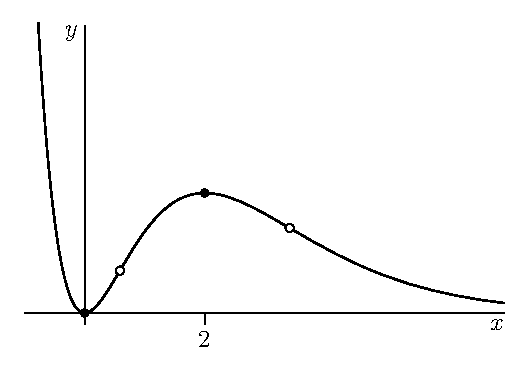
\includegraphics{graphE11}
%\end{center}
Open dots indicate inflection points, and closed dots indicate local extrema.
\begin{center}\begin{tikzpicture}[scale=1.2]
\YEaaxis{1}{6.2}{.25}{4}
\draw[thick] plot[domain=-.72:6, samples=100](\x,{3.7*\x*\x*exp(-\x)});
\draw (0,0) node[vertex]{};
\draw (2,2) node[vertex]{};
\draw (0.59,0.7) node[opendot]{};
\draw (3.4,1.4) node[opendot]{};
\YExcoord{2}{2}
\YExcoord{0.59}{2-\sqrt 2}
\YExcoord{3.4}{2+\sqrt 2}
\end{tikzpicture}\end{center}
\end{answer}
\begin{solution}
The parts of the question are just scaffolding to lead you through sketching the curve. Their answers are given explicitly, in an organized manner, in the ``answers" section. In this solution, they are scattered throughout.
\begin{itemize}
\item Asymptotes:

Since the function has a derivative at every real number, the function is continuous for every real number, so it has no vertical asymptotes. In the problem statement, you are told $\ds\lim_{x \to \infty} f(x)=0$, so $y=0$ is a horizontal asymptote as $x$ goes to infinity.  It remains to evaluate $\ds\lim_{x \to -\infty} f(x)$. Let's consider the limit of $f'(x)$ instead. Recall $K$ is a positive constant.
\begin{align*}
&\lim_{x \to -\infty}e^{-x}=\lim_{x \to \infty}e^x=\infty\\
&\lim_{x \to -\infty}K(2x-x^2)=-\infty
\intertext{So,}
&\lim_{x \to -\infty} K(2x-x^2)e^{-x}=-\infty
\end{align*}
That is, as $x$ becomes a hugely negative number, $f'(x)$ also becomes a hugely negative number. As we move left along the $x$-axis, $f(x)$ is decreasing with a steeper and steeper slope, as in the sketch below. That means
$\ds\lim_{x \to -\infty}f(x)=\infty$.
\begin{center}\begin{tikzpicture}
\YEaaxis{6}{1}{1}{8}
\draw[thick] (-1,1)--(-2,2) (-2.5,2.5)--(-3.5,4.5) (-3.75,5)--(-4.5,8);
\draw (-1.5,1.5) node[vertex]{};
\draw (-3,3.5) node[vertex]{};
\draw (-4.125,6.5) node[vertex]{};
\draw (-3,-1.5) node{Sketch: various tangent lines to $f(x)$,};
\draw (-3,-2) node{their slopes getting more strongly negative};
\draw (-3,-2.5) node{as $x$ gets more strongly negative.};
\end{tikzpicture}\end{center}
\item Intervals of increase and decrease:

We are given $f'(x)$ (although we don't know $f(x)$):
\[f'(x)=Kx(2-x)e^{-x}\]
The critical points of $f(x)$ are $x=0$ and $x=2$, and there are no singular points. Recall $e^{-x}$ is always positive, and $K$ is a positive constant.
\begin{center}\begin{tabular}{|c||c|c|c|c|c|}
\hline
$x$&$(-\infty,0)$&0&$(0,2)$&2&$(2,\infty)$\\
\hline
$f'(x)$&negative&0&positive&0&negative\\
\hline
$f(x)$& decreasing & local min & increasing & local max & decreasing\\
\hline
\end{tabular}\end{center}
So, $f(0)=0$ is a local minimum, and $f(2)=2$ is a local maximum.

Looking ahead to part \eqref{s3.6K4}, we have a skeleton of the curve.

\begin{center}\begin{tikzpicture}
\YEaaxis{4}{5.2}{.75}{4}
\draw[thick] (-4,4)--(0,0)--(2,2)--(4,.5)--(5,.25);
\draw (0,0) node[vertex]{};
\draw (2,2) node[vertex]{};
\draw[blue, decorate, decoration={brace, amplitude=10pt, mirror}] (-4,-1)--(0,-1);
\draw[blue] (-2,-1.75) node{decreasing};
\draw[red, decorate, decoration={brace, amplitude=10pt, mirror}] (0,-1)--(2,-1);
\draw[red] (1,-1.75) node{increasing};
\draw[blue, decorate, decoration={brace, amplitude=10pt, mirror}] (2,-1)--(4,-1);
\draw[blue] (3,-1.75) node{decreasing};
\YExcoord{2}{2}
\end{tikzpicture}\end{center}

\item Concavity:

Since we're given $f'(x)$, we can find $f''(x)$.
\begin{align*}
f''(x)&=K(2-2x-2x+x^2)e^{-x}\\
&=K(2-4x+x^2)e^{-x}\\
&=K\big(x-2-\sqrt{2}\big)\big(x-2+\sqrt{2}\big)e^{-x}
\end{align*}
where the last line can be found using the quadratic equation. So,
$f''(x)=0$  for $x=2\pm\sqrt{2}$, and $f''(x)$ exists everywhere.

\begin{center}\begin{tabular}{|c||c|c|c|c|c|}
\hline
$x$&$(-\infty,2-\sqrt{2})$&$2-\sqrt{2}$&$(2-\sqrt{2},2+\sqrt{2})$&$2+\sqrt 2$&$(2+\sqrt 2,\infty)$\\
\hline
$f'(x)$&positive&0&negative&0&positive\\
\hline
$f(x)$& concave up & IP & concave down & IP & concave up\\
\hline
\end{tabular}\end{center}

Now, we can add concavity to our sketch.

\begin{center}\begin{tikzpicture}[scale=1.2]
\YEaaxis{1}{6.2}{.25}{4}
\draw[thick] plot[domain=-.72:6, samples=100](\x,{3.7*\x*\x*exp(-\x)});
\draw (0,0) node[vertex]{};
\draw (2,2) node[vertex]{};
\draw (0.59,0.7) node[opendot]{};
\draw (3.4,1.4) node[opendot]{};
\YExcoord{2}{2}
\YExcoord{0.59}{2-\sqrt 2}
\YExcoord{3.4}{2+\sqrt 2}
\draw[blue, decorate, decoration={brace, amplitude=8pt, mirror}] (-1,-1)--(0,-1);
\draw[blue] (-.5,-1.5) node{decr};
\draw[red, decorate, decoration={brace, amplitude=10pt, mirror}] (0,-1)--(2,-1);
\draw[red] (1,-1.5) node{increasing};
\draw[blue, decorate, decoration={brace, amplitude=10pt, mirror}] (2,-1)--(6,-1);
\draw[blue] (4,-1.5) node{decreasing};
\draw[red, decorate, decoration={brace, amplitude=10pt, mirror}] (-1,-2.25)--(.59,-2.25);
\draw[red] (-.2,-2.75) node{cc up};
\draw[blue, decorate, decoration={brace, amplitude=10pt, mirror}] (.59,-2.25)--(3.4,-2.25);
\draw[blue] (2,-2.75) node{concave down};
\draw[red, decorate, decoration={brace, amplitude=10pt, mirror}] (3.4,-2.25)--(6,-2.25);
\draw[red] (4.7,-2.75) node{concave up};
\end{tikzpicture}\end{center}
%\begin{center}
%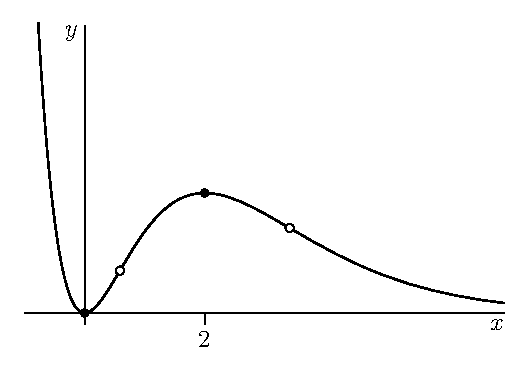
\includegraphics{graphE11}
%\end{center}
\end{itemize}
\end{solution}

\begin{question}[2010H]
 Let $f(x) = e^{-x}$ , $x \ge 0$.
\begin{enumerate}[(a)]
\item\label{s3.62010exp1} Sketch the graph of the equation $y = f(x)$. Indicate any
local extrema and inflection points.
\item\label{s3.62010exp4} Sketch the graph of  the inverse function $y = g (x)=f^{-1}(x)$.
\item\label{s3.62010exp2} Find the domain and range of the inverse function $g(x)= f^{-1}(x)$.
\item\label{s3.62010exp3} Evaluate $g'(\half)$.
\end{enumerate}
\end{question}
\begin{hint}
Once you have the graph of a function, reflect it over the line $y=x$ to graph its inverse.
Be careful of the fact that $f(x)$ is only defined in this problem for $x \geq 0$.
\end{hint}
\begin{answer}
\eqref{s3.62010exp1}
\begin{center}\begin{tikzpicture}
\YEaaxis{2}{6}{1}{6}
\draw[thick] plot[domain=0:5.5, samples=100](\x,{exp(-\x)}) node[above]{$y=f(x)$};
\YEycoord{1}{1};
\YExcoord{1}{1};
\draw (0,1) node[vertex]{};
\end{tikzpicture}\end{center}
There are no inflection points or extrema, except the endpoint $(0,1)$.

\eqref{s3.62010exp4}

\begin{center}\begin{tikzpicture}
\YEaaxis{2}{6}{2}{6}
\draw[thick, blue] plot[domain=0:5.5, samples=100]({exp(-\x)},\x) ;
\draw[blue] (1,1)node[right]{$y=g(x)$};
\YEycoord{1}{1};
\YExcoord{1}{1};
\draw[blue](1,0) node[vertex]{};
\end{tikzpicture}\end{center}
There are no inflection points or extrema, except the endpoint $(1,0)$.

\eqref{s3.62010exp2}
The domain of $g$ is  $(0,1]$.
The range of $g$ is $[0,\infty)$.

\eqref{s3.62010exp3}
$g'(\half)=-2$
\end{answer}
\begin{solution}
\eqref{s3.62010exp1}
You should be familiar with the graph of $y=e^x$. You can
           construct the graph of $y=e^{-x}$ just by reflecting the graph
           of $y=e^x$ across the $y$--axis. To see why this is the case,
           imagine swapping each value of $x$ its negative: for example,
                      swapping the point at $x = -1$ with the point at $x = 1$, etc.
           Alternatively, you can graph $y=f(x)=e^{-x}$, $x\ge 0$,
           using the methods of this section: at $x=0$, $y=f(0)=1$;
           as $x$ increases, $y=f(x)=e^{-x}$ decreases, with no local
           extrema; and as $x\rightarrow+\infty$, $y=f(x)\rightarrow 0$.

There are no inflection points or extrema, except the endpoint $(0,1)$.

\begin{center}\begin{tikzpicture}
\YEaaxis{2}{6}{1}{6}
\draw[thick, red] plot[domain=0:5.5, samples=100](\x,{exp(-\x)}) node[above]{$y=f(x)$};
\YEycoord{1}{1};
\YExcoord{1}{1};
\draw[red] (0,1) node[vertex]{};
\end{tikzpicture}\end{center}

\eqref{s3.62010exp4}

Recall that, to graph the inverse of a function, we reflect the original function across the line $y=x$.

You should be familiar with the graph of $y=e^x$. You can
           construct the graph of $y=e^{-x}$ just by reflecting the graph
           of $y=e^x$ across the $y$--axis. To see why this is the case,
           imagine swapping each value of $x$ its negative: for example,
           swapping the point at $x = -1$ with the point at $x = 1$, etc.

           Alternatively, you can graph $y=f(x)=e^{-x}$, $x\ge 0$,
           using the methods of this section: at $x=0$, $y=f(0)=1$;
           as $x$ increases, $y=f(x)=e^{-x}$ decreases, with no local
           extrema; and as $x\rightarrow+\infty$, $y=f(x)\rightarrow 0$.


           To see why this is true, consider the following. Since $g(x)$
           is the inverse of $f(x)$, then, for any pair of numbers $x$ and
           $y$, we have
           \begin{equation*}
                  f(x) = y\text{ if and only  }g(y) = x
          \end{equation*}
           That is, $g$ is the function that swaps the input and output
           of $f$. Now the point $(x,y)$ lies on the graph of $f$
           if and only if $y=f(x)$. Similarly, the point $(X,Y)$ lies
           on the graph of $g$ if and only if $Y=g(X)$. Setting $Y=x$
           and $X=y$ we see that the point $(y,x)$ lies on the graph of
           $g$ if and only if $x=g(y)$, which in turn is the case
           if and only if $y=f(x)$. So
           \begin{equation*}
                 \text{$(y,x)$ is on the graph of $g$ if and only
                        if $(x,y)$ is on the graph of $f$.}
           \end{equation*}
           To get from the point $(x,y)$ to the point $(y,x)$ we have to
           exchange $x \leftrightarrow y$, which we can do by reflecting
           over the line $y=x$.  Thus we can construct the graph of $g$
           by reflecting the curve $y = f(x)$ over the line  $y = x$.


\begin{center}\begin{tikzpicture}
\YEaaxis{2}{6}{2}{6}
\draw[thick, dashed, red] plot[domain=0:5.5, samples=100](\x,{exp(-\x)}) node[above]{$y=f(x)$};
\draw[dashed] (-2,-2)--(6,6) node[right]{$y=x$};
\draw[thick, blue] plot[domain=0:5.5, samples=100]({exp(-\x)},\x) ;
\draw[blue] (0,5)node[right]{$y=g(x)$};
\YEycoord{1}{1};
\YExcoord{1}{1};
\draw[red] (0,1) node[vertex]{};
\draw[blue] (1,0) node[vertex]{};
\end{tikzpicture}\end{center}

\eqref{s3.62010exp2}
The domain of $g$ is the range of $f$, which is $(0,1]$.
The range of $g$ is the domain of $f$, which is $[0,\infty)$.

\eqref{s3.62010exp3}
Since $g$ and $f$ are inverses,
\begin{align*}
g(f(x))&=x
\intertext{Using the chain rule,}
g'(f(x))\cdot f'(x)&=1
\intertext{Since $f'(x)=-e^{-x}=-f(x)$:}
g'(f(x))\cdot f(x)&=-1
\intertext{We plug in $f(x)=\frac{1}{2}$.}
g'\left(\frac{1}{2}\right)\cdot \frac{1}{2}&=-1\\
g'\left(\frac{1}{2}\right)&=-2
\end{align*}
\end{solution}




\begin{question}[2011H]
\begin{enumerate}[(a)]
\item Sketch the graph of $y=f(x)=x^5-x$, indicating asymptotes,
local maxima and minima, inflection points, and where the
graph is concave up/concave down.

\item Consider the function $f(x)=x^5-x+k$, where $k$ is a constant,
$-\infty<k<\infty$. How many roots does the function have? (Your answer might
depend on the value of $k$.)
\end{enumerate}
\end{question}
\begin{hint}

\end{hint}
\begin{answer}
(a)
\begin{center}\begin{tikzpicture}
\YEaxis{4}{4}
\draw[thick] plot[domain=-1.3:1.3, yscale=1.5, xscale=3, samples=100](\x,{\x*\x*\x*\x*\x-\x});
\draw (-2,.2) --(-2,-.2)node[below]{$\frac{-1}{\sqrt[4]{5}}$};
\draw (2,-.2) --(2,.2)node[above]{$\frac{1}{\sqrt[4]{5}}$};
\draw (.2,.78)--(-.2,.78) node[left]{$\frac{4}{5\sqrt[4]{5}}$};
\draw (.2,-.78)--(-.2,-.78) node[left]{$\frac{-4}{5\sqrt[4]{5}}$};
\end{tikzpicture}\end{center}
Local extrema are shown; inflection point at the origin.

(b) The number of distinct real roots of $x^5-x+k$ is:
\begin{itemize}
\item 1 when $|k|>\dfrac{4}{5\root{4}\of{5}}$
\item 2 when $|k|=\dfrac{4}{5\root{4}\of{5}}$
\item 3 when $|k|<\dfrac{4}{5\root{4}\of{5}}$
\end{itemize}
\end{answer}
\begin{solution}
(a)
First, we differentiate.
\[
f(x) = x^5-x\qquad
f'(x)=5x^4-1\qquad
f''(x)=20x^3\qquad
\]
The function and its first derivative tells us the following:
\begin{itemize}
\item $\ds\lim_{x \to \infty} f(x)=\infty$, $\ds\lim_{x \to -\infty} f(x)=-\infty$
\item $f'(x)> 0$ (i.e. $f$ is increasing) for
   $|x|> \dfrac{1}{\root{4}\of{5}}$
\item{}$f'(x)=0$ (i.e. $f$ has critical points) for $x= \pm\dfrac{1}{\root{4}\of{5}} \approx \pm 0.67$
\item{}$f'(x)< 0$ (i.e. $f$ is decreasing) for $|x| < \dfrac{1}{\root{4}\of{5}}$
\item $f\left(\pm\dfrac{1}{\sqrt[4]{5}}\right)=\mp\dfrac{4}{5\sqrt[4]{5}}\approx\mp0.53$
\end{itemize}
This gives us a first idea of the shape of the graph.
\begin{center}\begin{tikzpicture}
\YEaxis{5}{3}
\draw[->, thick] (-5,-3)--(-2,1.5);
\draw[->, thick] (-2,1.5)--(2,-1.5);
\draw[->, thick] (2,-1.5)--(5,3);
\draw (-2,.2) --(-2,-.2)node[below]{$\frac{-1}{\sqrt[4]{5}}$};
\draw (2,.2) --(2,-.2)node[below]{$\frac{1}{\sqrt[4]{5}}$};
\draw (.2,1.5)--(-.2,1.5) node[left]{$\frac{4}{5\sqrt[4]{5}}$};
\draw (.2,-1.5)--(-.2,-1.5) node[left]{$\frac{-4}{5\sqrt[4]{5}}$};
\end{tikzpicture}\end{center}
We refine this skeleton using information from the second derivative.
\begin{itemize}
\item $f''(x)> 0$ (i.e. $f$ is concave up) for $x> 0$,
%\hskip0.7in\smash{\figplace{OE11D_4}{0 in}{-0.3 in}}
\item{}$f''(x)=0$ (i.e. $f$ has an inflection point) for $x=0$, and
\item{}$f''(x)< 0$ (i.e. $f$ is concave down) for $x<0$
\end{itemize}
Thus
\begin{itemize}
\item $f$ has no asymptotes
\item $f$ has a local maximum at $x=-\dfrac{1}{\root{4}\of{5}}$
           and  a local minimum at $x=\dfrac{1}{\root{4}\of{5}}$
\item $f$ has an inflection point at $x=0$
\item $f$ is concave down for $x<0$ and concave up for $x>0$
\end{itemize}

\begin{center}\begin{tikzpicture}
\YEaxis{4}{4}
\draw[thick] plot[domain=-1.3:1.3, yscale=1.5, xscale=3, samples=100](\x,{\x*\x*\x*\x*\x-\x});
\draw (-2,.2) --(-2,-.2)node[below]{$\frac{-1}{\sqrt[4]{5}}$};
\draw (2,-.2) --(2,.2)node[above]{$\frac{1}{\sqrt[4]{5}}$};
\draw (.2,.78)--(-.2,.78) node[left]{$\frac{4}{5\sqrt[4]{5}}$};
\draw (.2,-.78)--(-.2,-.78) node[left]{$\frac{-4}{5\sqrt[4]{5}}$};
\end{tikzpicture}\end{center}
\medskip
(b) The function
$x^5-x+k$ has a root at $x=x_0$ if and only if $x^5-x=-k$
  at $x=x_0$. So the number of distinct real roots of $x^5-x+k$ is the
  number of times the curve $y=x^5-x$ crosses the horizontal line $y=-k$.
  The local maximum of $x^5-x$ (when $x=-\dfrac{1}{\root{4}\of{5}}$)
  is $\dfrac{4}{5\root{4}\of{5}}$, and the local minimum of $x^5-x$
 (when $x=\dfrac{1}{\root{4}\of{5}}$) is $-\dfrac{4}{5\root{4}\of{5}}$.
  So, looking at the graph of $x^5-x$ above, we see that the number of distinct
  real roots of $x^5-x+k$ is
\begin{itemize}
\item 1 when $|k|>\dfrac{4}{5\root{4}\of{5}}$
\item 2 when $|k|=\dfrac{4}{5\root{4}\of{5}}$
\item 3 when $|k|<\dfrac{4}{5\root{4}\of{5}}$
\end{itemize}
\end{solution}



\begin{question}[2012H]
The hyperbolic trigonometric functions $\sinh(x)$ and
$\cosh(x)$ are defined by
$$
\sinh(x)=\dfrac{e^x-e^{-x}}{2}\qquad
\cosh(x)=\dfrac{e^x+e^{-x}}{2}
$$
They have many properties that are similar to corresponding properties
of $\sin(x)$ and $\cos(x)$. In particular, it is easy to see that
$$
\diff{}{x} \sinh(x)=\cosh(x)\qquad
\diff{}{x} \cosh(x)=\sinh(x)\qquad
\cosh^2(x)-\sinh^2(x)=1
$$
You may use these properties in your solution to this question.
\begin{enumerate}[(a)]
\item Sketch the graphs of $\sinh(x)$ and $\cosh(x)$.
\item Define inverse hyperbolic trigonometric functions
$\sinh^{-1}(x)$ and $\cosh^{-1}(x)$, carefully specifing their domains
of definition. Sketch the graphs of $\sinh^{-1}(x)$ and $\cosh^{-1}(x)$.
\item Find
$
\dfrac{d\hfill}{dx}\left\{ \cosh^{-1}(x)\right\}
$.
\end{enumerate}
\end{question}
\begin{hint}
For (a), don't be intimidated by the new names: we can graph these functions using the methods learned in this section.

For (b), remember that to define an inverse of a function, we need to restrict the domain of that function to an interval where it is one-to-one. Then to graph the inverse, we can simply reflect the original function over the line $y=x$.

For (c), set $y(x)=\cosh^{-1}(x)$, so $\cosh(y(x))=x$. The differentiate using the chain rule. To get your final answer in terms of $x$ (instead of $y$), use the identity $\cosh^2(y)-\sinh^2(y)=1$.
\end{hint}
\begin{answer}
(a)
\begin{center}
\begin{tikzpicture}
\YEaxis{3}{3}
\draw plot[domain=-3:3, scale=0.3](\x,{sinh(\x)});
\draw (2,3) node[right]{$y=\sinh x$};
\end{tikzpicture}
\begin{tikzpicture}
\YEaaxis{3}{3}{.5}{3}
\draw plot[domain=-3:3, scale=0.3](\x,{cosh(\x)});
\draw (2,3) node[right]{$y=\cosh x$};
\draw (.2,.3)--(-.4,.3) node[left]{1};
\draw (0,-3) node{};
\end{tikzpicture}\end{center}

(b)
For any real $x$, define $\sinh^{-1}(x)$ to be
the unique solution of $\sinh(y)=x$. For every $x\in[1,\infty)$, define $\cosh^{-1}(x)$ to be the
unique $y\in[0,\infty)$ that obeys $\cosh(y)=x$.

\begin{center}
\begin{tikzpicture}
\YEaxis{3}{2}
\draw[blue, very thick] plot[domain=-3:3, scale=0.3]({sinh(\x)},\x);
\draw[blue] (1.5,1.25) node[right]{$y=\sinh^{-1} x$};
\end{tikzpicture}\hfill
\begin{tikzpicture}
\YEaaxis{3}{3}{.5}{2}
\draw[blue, very thick] plot[domain=0:3, scale=0.3]({cosh(\x)},\x);
\draw[blue] (1.5,1.25) node[right]{$y=\cosh^{-1} x$};
\draw (0,-2) node{};
\end{tikzpicture}
\end{center}

(c) $\ds\diff{}{x}\{\cosh^{-1}(x)\}=\dfrac{1}{\sqrt{x^2-1}}$
\end{answer}
\begin{solution}

 (a)
 You might not be familiar with hyperbolic sine and cosine, but you don't need to be. We can graph them using  the same methods as the other curves in this section. The derivatives are given to us:
 \[\diff{}{x}\{\sinh x\}=\cosh x =\frac{e^x+e^{-x}}{2}\qquad\diff{}{x}\{\cosh x\}=\sinh x = \frac{e^x-e^{-x}}{2}\]
 \[\left(\diff{}{x}\right)^2\{\sinh x\}=\sinh x =\frac{e^x-e^{-x}}{2}\qquad
 \left(\diff{}{x}\right)^2\{\cosh x\}=\cosh x = \frac{e^x+e^{-x}}{2}\]
  Observe that:
 \begin{itemize}
 \item $\sinh(x)$ has a derivative that is always positive, so $\sinh(x)$ is always increasing. The second derivative of $\sinh(x)$ is negative to the left of $x=0$ and positive to the right of $x=0$, so $\sinh(x)$ is concave down to the left of the $y$-axis and concave up to its right, with an inflection point at $x=0$.
  \item $\cosh(x)$ has a derivative that is positive when $x>0$ and negative when $x<0$. The second derivative of $\cosh(x)$ is always positive, so it is always concave up.
\item $\cosh(0)=1$ and $\sinh(0)=0$.
\item
 $\ds\lim_{x\rightarrow\infty}\sinh x = \ds\lim_{x\rightarrow\infty}\cosh x
 =\ds\lim_{x\rightarrow\infty}\frac{e^x}{2}=\infty$, since $\ds\lim_{x \to \infty}e^{-x}=0$
\item
$\ds\lim_{x \to -\infty}\sinh x =\ds\lim_{x \to -\infty}\left(\frac{e^x}{2}-\frac{e^{-x}}{2}\right)
=\ds\lim_{x \to \infty}\left(\frac{e^{-x}}{2}-\frac{e^x}{2}\right)=-\infty
$ and\\
$\ds\lim_{x \to -\infty}\cosh x =\ds\lim_{x \to -\infty}\left(\frac{e^x}{2}+\frac{e^{-x}}{2}\right)
=\ds\lim_{x \to \infty}\left(\frac{e^{-x}}{2}+\frac{e^x}{2}\right)=\infty
$
\item $\cosh(x)$ is even, since $\cosh(-x)=\dfrac{e^{-x}+e^{-(-x)}}{2}=\dfrac{e^{-x}+e^x}{2}=\cosh (x)$, and\\
$\sinh (x)$ is odd, since $\sinh(-x)=\dfrac{e^{-x}-e^{-(-x)}}{2}=\dfrac{e^{-x}-e^x}{2}=\dfrac{-\left(e^x-e^{-x}\right)}{2}=-\sinh(x)$
\end{itemize}

\begin{center}
\begin{tikzpicture}
\YEaxis{3}{3}
\draw plot[domain=-3:3, scale=0.3](\x,{sinh(\x)});
\draw (2,3) node[right]{$y=\sinh x$};
\end{tikzpicture}
\begin{tikzpicture}
\YEaaxis{3}{3}{.5}{3}
\draw plot[domain=-3:3, scale=0.3](\x,{cosh(\x)});
\draw (2,3) node[right]{$y=\cosh x$};
\draw (.2,.3)--(-.4,.3) node[left]{1};
\draw (0,-3) node{};
\end{tikzpicture}\end{center}


(b)
\begin{itemize}\item As $y$ runs over $(-\infty,\infty)$ the function
$\sinh(y)$ takes every real value exactly once. So,
for each $x\in(-\infty,\infty)$, define $\sinh^{-1}(x)$ to be
the unique solution of $\sinh(y)=x$.
\item As $y$ runs over $[0,\infty)$ the function
$\cosh(y)$ takes every real value in $[1,\infty)$ exactly once.
In particular, the smallest value of $\cosh(y)$ is $\cosh(0)=1$.
So, for each $x\in[1,\infty)$, define $\cosh^{-1}(x)$ to be the
unique $y\in[0,\infty)$ that obeys $\cosh(y)=x$.
\end{itemize} To graph the inverse of a (one-to-one) function, we reflect the original function over the line $y=x$. Using this method to graph $y=\sinh^{-1}(x)$ is straightforward. To graph $y=\cosh(x)$, we need to be careful of the domains: we are restricting $\cosh(x)$ to values of $x$ in $[0,\infty)$.
The graphs are

\begin{center}
\begin{tikzpicture}
\YEaxis{3}{3}
\draw[red, thin] plot[domain=-3:3, scale=0.3](\x,{sinh(\x)});
\draw[red] (1,3) node[below right]{$y=\sinh x$};
\draw[dashed] (-3,-3)--(2,2);% node[right]{$y=x$};
\draw[blue, very thick] plot[domain=-3:3, scale=0.3]({sinh(\x)},\x);
\draw[blue] (1.5,1.25) node[right]{$y=\sinh^{-1} x$};
\draw[ultra thick, ->] (4,0)--(5,0);
\end{tikzpicture}
\begin{tikzpicture}
\YEaxis{3}{3}
\draw[blue, very thick] plot[domain=-3:3, scale=0.3]({sinh(\x)},\x);
\draw[blue] (1.5,1.25) node[right]{$y=\sinh^{-1} x$};
\end{tikzpicture}

\begin{tikzpicture}
\YEaaxis{3}{3}{.5}{2}
\draw[red, thin] plot[domain=0:3, scale=0.3](\x,{cosh(\x)});
\draw[red] (1,3) node[below right]{$y=\cosh x$};
\draw[dashed] (-1,-1)--(2,2);% node[right]{$y=x$};
\draw[blue, very thick] plot[domain=0:3, scale=0.3]({cosh(\x)},\x);
\draw[blue] (1.5,1.25) node[right]{$y=\cosh^{-1} x$};
\draw[ultra thick, ->] (4,1)--(5,1);
\end{tikzpicture}
\begin{tikzpicture}
\YEaaxis{3}{3}{.5}{2}
\draw[blue, very thick] plot[domain=0:3, scale=0.3]({cosh(\x)},\x);
\draw[blue] (1.5,1.25) node[right]{$y=\cosh^{-1} x$};
\draw (-1,-1) node{};
\end{tikzpicture}
\end{center}
%\centerline{\figput{graphE12A}\hskip1in\figplace{graphE12B}{0in}{0.5in}}

\item{}(c) Let $y(x)= \cosh^{-1}(x)$. Then, using the definition of $\cosh^{-1}$,
\begin{align*}
\cosh y(x)&=x
\intertext{We differentiate with respect to $x$ using the chain rule.}
\diff{}{x}\left\{\cosh y(x)\right\}&=\diff{}{x}\{x\}\\
y'(x) \sinh y(x)&=1
\intertext{We solve for $y'(x)$.}
y'(x) &=\dfrac{1}{\sinh y(x)}
\intertext{We want to have our answer in terms of $x$, not $y$. We know that $\cosh y=x$, so if we can convert hyperbolic sine into hyperbolic cosine, we can get rid of $y$. Our tool for this is the identity, given in the question statement, $\cosh^2(x)-\sinh^2(x)=1$. This tells us $\sinh^2(y)=1-\cosh^2(y)$.
Now we have to decide whether $\sinh(y)$ is the positive or negative square root of $1-\cosh^2(y)$ in our context. Looking at the graph of $y(x)=\cosh^{-1}(x)$, we see $y'(x)>0$. So we use the positive square root:}
y'(x) & =\dfrac{1}{\sqrt{\cosh^2 y(x)-1}}
  =\dfrac{1}{\sqrt{x^2-1}}
\end{align*}
Remark: $\ds\diff{}{x}\left\{\arccos(x)\right\}=\dfrac{-1}{\sqrt{1-x^2}}$, so again the hyperbolic trigonometric function has properties similar to (but not exactly the same as) its trigonometric counterpart.
\end{solution}

%%%%%
\section{L'H\^opital's Rule and indeterminate forms}
%
% Copyright 2018 Joel Feldman, Andrew Rechnitzer and Elyse Yeager.
% This work is licensed under a Creative Commons Attribution-NonCommercial-ShareAlike 4.0 International License.
% https://creativecommons.org/licenses/by-nc-sa/4.0/
%
\questionheader{ex:s3.7}
%%%%%%%%%%%%%%%%%%
\subsection*{\Conceptual}
%%%%%%%%%%%%%%%%%%
\Instructions{In Questions~\ref{s3.7indet1} to \ref{s3.7indet3}, you are asked to give pairs of functions that combine to make indeterminate forms. Remember that an indeterminate form is indeterminate precisely because its limit can take on a number of values.}

\begin{Mquestion}\label{s3.7indet1}
Give two functions $f(x)$ and $g(x)$ with the following properties:
\begin{enumerate}[(i)]
\item $\ds\lim_{x \to \infty} f(x)=\infty$
\item $\ds\lim_{x \to \infty} g(x)=\infty$
\item $\ds\lim_{x \to \infty} \dfrac{f(x)}{g(x)}=2.5$
\end{enumerate}
\end{Mquestion}
\begin{hint} Try making one function a multiple of the other.
\end{hint}
\begin{answer} There are many possible answers. Here is one: $f(x)=5x$, $g(x)=2x$.
\end{answer}
\begin{solution} There are many possible answers. Consider these: $f(x)=5x$, $g(x)=2x$.
Then $\ds\lim_{x \rightarrow\infty}f(x)=\ds\lim_{x\to\infty}g(x)=\infty$, and
$\ds\lim_{x\to\infty}\frac{f(x)}{g(x)}=\ds\lim_{x\to\infty}\frac{5x}{2x}=\ds\lim_{x\to\infty}\frac{5}{2}=\frac{5}{2}=2.5$.
\end{solution}


\begin{Mquestion}Give two functions $f(x)$ and $g(x)$ with the following properties:
\begin{enumerate}[(i)]
\item $\ds\lim_{x \to \infty} f(x)=\infty$
\item $\ds\lim_{x \to \infty} g(x)=\infty$
\item $\ds\lim_{x \to \infty} \dfrac{f(x)}{g(x)}=0$
\end{enumerate}
\end{Mquestion}
\begin{hint} Try making one function a multiple of the other, but not a \emph{constant} multiple.
\end{hint}
\begin{answer} There are many possible answers. Here is one: $f(x)=x$, $g(x)=x^2$.
\end{answer}
\begin{solution} There are many possible answers. Consider these: $f(x)=x$, $g(x)=x^2$.
Then $\ds\lim_{x \rightarrow\infty}f(x)=\ds\lim_{x\to\infty}g(x)=\infty$, and
$\ds\lim_{x\to\infty}\frac{f(x)}{g(x)}=\ds\lim_{x\to\infty}\frac{x}{x^2}=\ds\lim_{x\to\infty}\frac{1}{x}=0$.
\end{solution}




\begin{Mquestion}\label{s3.7indet3}
Give two functions $f(x)$ and $g(x)$ with the following properties:
\begin{enumerate}[(i)]
\item\label{s3.7conc1} $\ds\lim_{x \to \infty} f(x)=1$
\item\label{s3.7conc2} $\ds\lim_{x \to \infty} g(x)=\infty$
\item\label{s3.7conc3} $\ds\lim_{x \to \infty} [f(x)]^{g(x)}=5$
\end{enumerate}
\end{Mquestion}
\begin{hint} Try modifying the function from Example~\ref*{eg:hopitalL}.%Examplt 3.7.20
\end{hint}
\begin{answer} There are many possible answers. Here is one: $f(x)=1+\frac{1}{x}$, $g(x)=x\log 5$ (recall we use $\log$ to mean logarithm base $e$).
\end{answer}
\begin{solution}
From Example~\ref*{eg:hopitalL}, we know that $\ds\lim_{x \to 0} (1+x)^{\frac{a}{x}}=e^a$, so $\ds\lim_{x \to 0} (1+x)^{\frac{\log 5}{x}}=e^{\log 5}=5$. However, this is the limit as $x$ goes to 0, which is not what we were asked. So, we modify the functions by replacing $x$ with $\frac{1}{x}$. If $x \to 0^+$, then $\frac{1}{x} \to \infty$.

Taking $f(x)=1+\frac{1}{x}$ and $g(x)=x\log 5$, we see:\\
\eqref{s3.7conc1} $\ds\lim_{x \to \infty} f(x)=\ds\lim_{x \to \infty } \left(1+\frac{1}{x}\right)=1$\\
\eqref{s3.7conc2} $\ds\lim_{x \to \infty} g(x)=\ds\lim_{x \to \infty} x\log 5=\infty$\\
\eqref{s3.7conc3} Let us name $\dfrac{1}{x}=X$. Then as $x \to \infty$, $X \to 0^+$, so:\\
 $\ds\lim_{x \to \infty} [f(x)]^{g(x)}=\ds\lim_{x \to \infty} \left[1+\frac{1}{x}\right]^{x\log 5}=\lim_{x \to \infty} \left[1+\frac{1}{x}\right]^{\frac{\log 5}{\frac{1}{x}}}=
\lim_{X \to 0^+} \left[1+X\right]^{\frac{\log 5}{X}}=e^{\log 5}=5
$,
where in the penultimate step, we used  the result of Example~\ref*{eg:hopitalL}.
\end{solution}
%%%%%%%%%%%%%%%%%%
\subsection*{\Procedural}
%%%%%%%%%%%%%%%%%%


\begin{Mquestion}[2009H]
Evaluate $\lim\limits_{x\rightarrow 1}\dfrac{x^3-e^{x-1}}{\sin(\pi x)}$.
\end{Mquestion}
\begin{hint}
Plugging in $x=1$ to the numerator and denominator makes both zero. This is exactly one of the indeterminate forms where l'H\^opital's rule can be directly applied.
\end{hint}
\begin{answer}  $-\dfrac{2}{\pi}$
\end{answer}
\begin{solution}
If we plug in $x=1$ to the numerator and the denominator, we find they are both zero. So, we have an indeterminate form appropriate for L'H\^opital's Rule.
\begin{align*}
\lim\limits_{x\rightarrow 1}\underbrace{\frac{x^3-e^{x-1}}{\sin(\pi x)}}_{\atp
	{\mathrm{num} \to 0}
	{\mathrm{den} \to 0}}
=\lim\limits_{x\rightarrow 1}\frac{3x^2-e^{x-1}}{\pi\cos(\pi x)}
=-\frac{2}{\pi}\end{align*}
\end{solution}


\begin{question}[2010H]
Evaluate $\lim\limits_{x\rightarrow 0+}\dfrac{\log x}{x}$. (Remember: in these notes, $\log$ means logarithm base $e$.)
\end{question}
\begin{hint}
Is this an indeterminate form?
\end{hint}
\begin{answer} $-\infty$
\end{answer}
\begin{solution}
Be careful-- this is not an indeterminate form!
\medskip

As $x\rightarrow 0+$, the numerator $\log x\rightarrow-\infty$. That is, the numerator is becoming an increasingly huge, negative number.
As $x\rightarrow 0+$, the denominator $x\rightarrow 0+$, which only serves to make the total fraction even larger, and still negative. So, $\lim\limits_{x\rightarrow 0^+}\dfrac{\log x}{x}
=-\infty$.
\medskip

Remark: if we had tried to use l'H\^opital's Rule here, we would have come up with the wrong answer. If we differentiate the numerator and the denominator, the fraction becomes $\dfrac{\frac{1}{x}}{1}=\frac{1}{x}$, and $\ds\lim_{x \to 0^+}\frac{1}{x}=\infty$. The reason we cannot apply l'H\^opital's Rule is that we do not have an indeterminate form, like both numerator and denominator going to infinity, or both numerator and denominator going to zero.
\end{solution}



\begin{question}[2012H]
Evaluate $\lim\limits_{x\rightarrow\infty}(\log x)^2e^{-x}$.
\end{question}
\begin{hint}
First, rearrange the expression to a more natural form (without a negative exponent).
\end{hint}
\begin{answer}
0
\end{answer}
\begin{solution}
We rearrange the expression to a more natural form:
\begin{align*}
\lim_{x\rightarrow\infty}(\log x)^2e^{-x}
&=\lim_{x\rightarrow\infty}\underbrace{\dfrac{(\log x)^2}{e^{x}}}_{\atp
	{\mathrm{num}\to\infty}
	{\mathrm{den}\to\infty}}
\intertext{If we plug in $x=0$, both numerator and denominator go to infinity. So, we can apply l'H\^opital's Rule. In fact, we end up applying it twice.}
&=\lim_{x\rightarrow\infty}\underbrace{\dfrac{2\log x}{xe^{x}}}_{\atp
	{\mathrm{num}\to\infty}
	{\mathrm{den}\to\infty}}
\\
&=\lim_{x\rightarrow\infty}\dfrac{2/x}{xe^{x}+e^x}
\intertext{The numerator gets smaller and smaller while the denominator gets larger and larger, so:}
&={0}
\end{align*}

\end{solution}

\begin{question}[1997D]
Evaluate
$\lim\limits_{x\rightarrow\infty}x^2e^{-x}$.
\end{question}
\begin{hint} If at first you don't succeed, try, try again.
\end{hint}
\begin{answer} 0
\end{answer}
\begin{solution}
$$
\lim_{x\rightarrow\infty}x^2e^{-x}
=\lim_{x\rightarrow\infty}\underbrace{\frac{x^2}{e^{x}}}_{\atp
	{\mathrm{num}\to \infty}
	{\mathrm{den}\to \infty}}
=\lim_{x\rightarrow\infty}\underbrace{\frac{2x}{e^{x}}}_{\atp
	{\mathrm{num}\to\infty}
	{\mathrm{den}\to\infty}}
=\lim_{x\rightarrow\infty}\underbrace{\frac{2}{e^{x}}}_{\atp
	{\mathrm{num}\to\infty}
	{\mathrm{den}\to\infty}}
={0}
$$

\end{solution}


\begin{question}[1997D]
Evaluate $\lim\limits_{x\rightarrow 0}\dfrac{x-x\cos x}{x-\sin x}$.
\end{question}
\begin{hint} Keep at it!
\end{hint}
\begin{answer} 3
\end{answer}
\begin{solution}
\begin{align*}
\lim_{x\rightarrow 0}\underbrace{\frac{x-x\cos x}{x-\sin x}}_{\atp
	{\mathrm{num}\to0}
	{\mathrm{den}\to0}}
&= \lim_{x\rightarrow 0}\underbrace{\frac{1-\cos x+x\sin x}{1-\cos x}}_{\atp
	{\mathrm{num}\to0}
	{\mathrm{den}\to0}}
= \lim_{x\rightarrow 0}\underbrace{\frac{\sin x+\sin x+x\cos x}{\sin x}}_{\atp
	{\mathrm{num}\to0}
	{\mathrm{den}\to0}}\\
&= \lim_{x\rightarrow 0}\frac{2\cos x+\cos x-x\sin x}{\cos x}
={3}
\end{align*}
\end{solution}




\begin{question}
Evaluate
$\ds\lim_{x \to 0}\dfrac{\sqrt{x^6+4x^4}}{x^2\cos x}$.
\end{question}
\begin{hint} Rather than use l'H\^opital, try factoring out $x^2$ from the numerator and denominator.
\end{hint}
\begin{answer}
$2$
\end{answer}
\begin{solution}
If we plug in $x=0$ to the numerator and denominator, both are zero, so this is a candidate for l'H\^opital's Rule. However, an easier way to evaluate the limit is to factor $x^2$ from the numerator and denominator, and cancel.
\begin{align*}
\lim_{x\to0}\frac{\sqrt{x^6+4x^4}}{x^2\cos x}
&=\lim_{x\to0}\frac{\sqrt{x^4}\sqrt{x^2+4}}{x^2\cos x}\\
&=\lim_{x\to0}\frac{x^2\sqrt{x^2+4}}{x^2\cos x}\\
&=\lim_{x\to0}\frac{\sqrt{x^2+4}}{\cos x}\\
&=\frac{\sqrt{0^2+4}}{\cos(0)}=2
\end{align*}
\end{solution}

\begin{question}[1997A]
Evaluate $\lim\limits_{x\rightarrow\infty}\dfrac{(\log x)^2}{x}$.
\end{question}
\begin{hint} Keep going!
\end{hint}
\begin{answer} 0
\end{answer}
\begin{solution}
\begin{align*}\lim_{x\rightarrow\infty}\underbrace{\frac{(\log x)^2}{x}}_{\atp
	{\mathrm{num}\to\infty}
	{\mathrm{den}\to\infty}}
&=\lim_{x\rightarrow\infty}\frac{2(\log x)\frac{1}{x}}{1}
=2\lim_{x\rightarrow\infty}\underbrace{\frac{\log x}{x}}_{\atp
	{\mathrm{num}\to\infty}
	{\mathrm{den}\to\infty}}
= 2\lim_{x\rightarrow\infty}\frac{\frac{1}{x}}{1}={0}
\end{align*}
\end{solution}


\begin{question}[1997A]
Evaluate $\lim\limits_{x\rightarrow0}\dfrac{1-\cos x}{\sin^2 x}$.
\end{question}
\begin{answer} $\frac{1}{2}$
\end{answer}
\begin{solution}
\begin{align*}
\lim_{x\rightarrow0}\underbrace{\frac{1-\cos x}{\sin^2 x}}_{\atp
	{\mathrm{num}\to0}
	{\mathrm{den}\to0}}
&= \lim_{x\rightarrow0}\frac{\sin x}{2\sin x\cos x}
=\lim_{x\rightarrow0}\frac{1}{2\cos x}
={\frac{1}{2}}
\end{align*}
\end{solution}




\begin{question}
Evaluate $\ds\lim_{x \to 0}\dfrac{x}{\sec x}$.
\end{question}
\begin{hint}
Try plugging in $x=0$. Is this an indeterminate form?
\end{hint}
\begin{answer} 0
\end{answer}
\begin{solution}
If we plug in $x=0$, the numerator is zero, and the denominator is \\
$\sec 0 = \dfrac{1}{\cos 0}=\dfrac{1}{1}=1$. So the limit is $\dfrac{0}{1}=0$.

\medskip
Be careful: you cannot use l'H\^opital's Rule here, because the fraction does not give an indeterminate form. If you try to differentiate the numerator and the denominator, you get an expression whose limit does not exist:\\
$\ds\lim_{x \to 0}\dfrac{1}{\sec x \tan x}=\ds\lim_{x \to 0}\cos x\cdot \dfrac{\cos x}{\sin x}=DNE$.
\end{solution}




\begin{Mquestion}
Evaluate $\ds\lim_{x\to0}\dfrac{\csc x\cdot \tan x\cdot (x^2+5)}{e^x}$.
\end{Mquestion}
\begin{hint}
Simplify the trigonometric part first.
\end{hint}
\begin{answer}
$5$
\end{answer}
\begin{solution}
If we plug $x=0$ into the denominator, we get 1. However, the numerator is an indeterminate form: $\tan 0 =0$,  while  $\ds\lim_{x \to 0^+}\csc x=\infty$ and
$\ds\lim_{x \to 0^-}\csc x=-\infty$. If we use $\csc x = \frac{1}{\sin x}$, our expression becomes
\begin{align*}
\lim_{x\to0}\frac{\tan x\cdot (x^2+5)}{\sin x \cdot e^x}&
\intertext{Since plugging in $x=0$ makes both the numerator and the denominator equal to zero, this is a candidate for l'H\^ospital's Rule. However, a much easier way is to simplify the trig first.}
\lim_{x\to0}\frac{\tan x\cdot (x^2+5)}{\sin x \cdot e^x}&=
\lim_{x\to0}\frac{\sin x\cdot (x^2+5)}{\cos x \cdot\sin x \cdot e^x}\\&=
\lim_{x\to0}\frac{x^2+5}{\cos x \cdot e^x}\\
&=\frac{0^2+5}{\cos(0)\cdot e^0}=5
\end{align*}
\end{solution}

\begin{Mquestion}Evaluate $\ds\lim_{x \to \infty}\sqrt{2x^2+1}-\sqrt{x^2+x}$.
\end{Mquestion}
\begin{hint} Rationalize, then remember your training.
\end{hint}
\begin{answer} $\infty$
\end{answer}
\begin{solution}
$\ds\lim_{x \to \infty}\sqrt{2x^2+1}-\sqrt{x^2+x}$ has the indeterminate form $\infty - \infty$. To get a better idea of what's going on, let's rationalize.
\begin{align*}
\lim_{x \to \infty}\sqrt{2x^2+1}-\sqrt{x^2+x}&=
\lim_{x \to \infty}\left(\sqrt{2x^2+1}-\sqrt{x^2+x}\right)\left(
\frac{\sqrt{2x^2+1}+\sqrt{x^2+x}}{\sqrt{2x^2+1}+\sqrt{x^2+x}}\right)\\
&=\lim_{x \to \infty}
\frac{(2x^2+1)-(x^2+x)}{\sqrt{2x^2+1}+\sqrt{x^2+x}}=
\lim_{x \to \infty}
\frac{x^2-x+1}{\sqrt{2x^2+1}+\sqrt{x^2+x}}
\intertext{Here, we have the indeterminate form $\frac{\infty}{\infty}$, so l'H\^opital's Rule applies. However, if we try to use it here, we quickly get a huge mess. Instead, remember how we dealt with these kinds of limits in the past: factor out the highest power of the denominator, which is $x$.}
&=\lim_{x \to \infty}
\frac{x\left(x-1+\frac{1}{x}\right)}{\sqrt{x^2(2+\frac{1}{x^2})}+\sqrt{x^2(1+\frac{1}{x})}}\\
&=\lim_{x \to \infty}
\frac{x\left(x-1+\frac{1}{x}\right)}{x\left(\sqrt{2+\frac{1}{x^2}}+\sqrt{1+\frac{1}{x}}\right)}\\
&=\lim_{x \to \infty}
\underbrace{\frac{x-1+\frac{1}{x}}{\sqrt{2+\frac{1}{x^2}}+\sqrt{1+\frac{1}{x}}}}_{\atp
	{\mathrm{num}\to \infty}
	{\mathrm{den}\to \sqrt{2}+1}}\\
&=\infty
\end{align*}
\end{solution}


\begin{question}[2010H]
Evaluate $\lim\limits_{x\rightarrow 0}\dfrac{\sin(x^3+3x^2)}{\sin^2x}$.
\end{question}
\begin{hint}
If it is too difficult to take a derivative for l'H\^opital's Rule, try splitting up the function into smaller chunks and evaluating their limits independently.
\end{hint}
\begin{answer} 3
\end{answer}
\begin{solution}
If we plug in $x=0$, both numerator and denominator become zero. So, we have exactly one of the indeterminate forms that l'H\^opital's Rule applies to.
\begin{align*}
\lim_{x\rightarrow 0}\underbrace{\dfrac{\sin(x^3+3x^2)}{\sin^2x}}_{\atp
	{\mathrm{num}\to0}
	{\mathrm{den}\to 0}}
&= \lim_{x\rightarrow 0}\dfrac{(3x^2+6x)\cos(x^3+3x^2)}{2\sin x\cos x}	\intertext{If we plug in $x=0$, still we find that both the numerator and the denominator go to zero. We could jump in with another iteration of l'H\^opital's Rule. However, the derivatives would be a little messy, so we use limit laws and break up the fraction into the product of two fractions. If both limits exist:}
\lim_{x\rightarrow 0}\dfrac{(3x^2+6x)\cos(x^3+3x^2)}{2\sin x\cos x}&=\left(\lim_{x\rightarrow 0}\dfrac{x^2+2x}{\sin x}\right)\cdot
\left(\lim_{x\rightarrow 0}\dfrac{3\cos(x^3+3x^2)}{2\cos x}\right)
\intertext{We can evaluate the right-hand limit by simply plugging in $x=0$:}
&=\dfrac{3}{2}\lim_{x\rightarrow 0}\underbrace{\dfrac{x^2+2x}{\sin x}}_
{\atp
	{\mathrm{num}\to0}
	{\mathrm{den}\to 0}}
\\
&= \dfrac{3}{2}\lim_{x\rightarrow 0}\dfrac{2x+2}{\cos x}\\
&=\frac{3}{2}\left(\frac{2}{1}\right)=3\end{align*}
\end{solution}



\begin{question}[1996D]
Evaluate $\lim\limits_{x\rightarrow1}\dfrac{\log(x^3)}{x^2-1}$.
\end{question}
\begin{answer} $\frac{3}{2}$
\end{answer}
\begin{solution}
$$
\lim_{x\rightarrow1}\frac{\log(x^3)}{x^2-1}
=\lim_{x\rightarrow1}\underbrace{\frac{3\log(x)}{x^2-1}}_{\atp
	{\mathrm{num}\to0}
	{\mathrm{den}\to0}}
=\lim_{x\rightarrow1}\frac{3/x}{2x}
=\frac{3}{2}
$$
\end{solution}

\begin{Mquestion}[1996D]
Evaluate $\lim\limits_{x\rightarrow 0}\dfrac{e^{-1/x^2}}{x^4}$.
\end{Mquestion}
\begin{hint} Try manipulating the function to get it into a nicer form
\end{hint}
\begin{answer} 0
\end{answer}
\begin{solution}
\begin{itemize}
\item Solution 1.
$$
\lim_{x\rightarrow 0}\frac{e^{-1/x^2}}{x^4}
=\lim_{x\rightarrow 0}\underbrace{\frac{\frac{1}{x^4}}{e^{1/x^2}}}_{\atp
	{\mathrm{num}\to\infty}
	{\mathrm{den}\to\infty}}
=\lim_{x\rightarrow 0}\frac{\frac{-4}{x^5}}{\frac{-2}{x^3}e^{1/x^2}}
=\lim_{x\rightarrow 0}\underbrace{\frac{\frac{2}{x^2}}{e^{1/x^2}}}_{\atp
	{\mathrm{num}\to\infty}
	{\mathrm{den}\to\infty}}
=\lim_{x\rightarrow 0}\frac{\frac{-4}{x^3}}{\frac{-2}{x^3}e^{1/x^2}}
=\lim_{x\rightarrow 0}\frac{2}{e^{1/x^2}}
={0}
$$
since, as $x\rightarrow 0$, the exponent $\frac{1}{x^2}\rightarrow\infty$
so that $e^{1/x^2}\rightarrow\infty$ and $e^{-1/x^2}\rightarrow 0$.
\item Solution 2.
$$
\lim_{x\rightarrow 0}\frac{e^{-1/x^2}}{x^4}
=\lim_{t={1\over x^2}\rightarrow \infty}\frac{e^{-t}}{t^{-2}}
=\lim_{t\rightarrow \infty}\underbrace{\frac{t^2}{e^{t}}}_{\atp
	{\mathrm{num}\to\infty}
	{\mathrm{den}\to\infty}}
=\lim_{t\rightarrow \infty}\underbrace{\frac{2t}{e^{t}}}_{\atp
	{\mathrm{num}\to\infty}
	{\mathrm{den}\to\infty}}
=\lim_{t\rightarrow \infty}\frac{2}{e^{t}}
={0}
$$
\end{itemize}
\end{solution}




\begin{question}[1998H]
Evaluate $\lim\limits_{x\rightarrow 0}
\dfrac{xe^x}{\tan (3x)}$.
\end{question}
\begin{answer} $\frac{1}{3}$
\end{answer}
\begin{solution} $$
\lim_{x\rightarrow 0}\underbrace{\frac{xe^x}{\tan (3x)}}_{\atp
	{\mathrm{num}\to0}
	{\mathrm{den}\to0}}
= \lim_{x\rightarrow 0}\frac{e^x+xe^x}{3\sec^2 (3x)}
=\frac{1}{3}
$$
\end{solution}



\begin{Mquestion}
Evaluate $\lim\limits_{x \to 0}\sqrt[x^2]{\sin^2 x}$.
\end{Mquestion}
\begin{hint} $\lim\limits_{x \to 0}\sqrt[x^2]{\sin^2 x}=(\sin^2 x)^{\frac{1}{x^2}}$; what form is this?
\end{hint}
\begin{answer} 0
\end{answer}
\begin{solution} $\ds\lim_{x \to 0} \sin^2 x = 0$, and $\ds\lim_{x \to 0}\frac{1}{x^2}=\infty$, so we have the form $0^\infty$. (Note that $\sin^2 x$ is positive, so our root is defined.) This is not an indeterminate form: $\lim\limits_{x \to 0}\sqrt[x^2]{\sin^2 x}=0$.
\end{solution}


\begin{Mquestion}
Evaluate $\lim\limits_{x \to 0}\sqrt[x^2]{\cos x}$.
\end{Mquestion}
\begin{hint} $\lim\limits_{x \to 0}\sqrt[x^2]{\cos x} = \ds\lim_{x \to 0}(\cos x)^{\frac{1}{x^2}}$
\end{hint}
\begin{answer} $\frac{1}{\sqrt{e}}$
\end{answer}
\begin{solution} $\ds\lim_{x \to 0} \cos x =1$ and $\ds\lim_{x \to 0}\frac{1}{x^2}=\infty$, so $\ds\lim_{x \to 0}(\cos x)^{\frac{1}{x^2}}$ has the indeterminate form $1^\infty$. We want to use l'H\^opital, but we need to get our function into a fractional indeterminate form. So, we'll use a logarithm.
\begin{align*}
y:&=(\cos x)^{\frac{1}{x^2}}\\
\log y &= \log \left((\cos x)^{\frac{1}{x^2}}\right)=\frac{1}{x^2}\log(\cos x)=\frac{\log \cos x}{x^2}\\
\lim_{x \to 0}\log y &=\lim_{x \to 0}\underbrace{\frac{\log \cos x}{x^2}}_{\atp
	{\mathrm{num}\to0}
	{\mathrm{den}\to 0}}
	=
	\lim_{x \to 0} \frac{\frac{-\sin x}{\cos x}}{2x}=
	\lim_{x \to 0} \underbrace{\frac{-\tan x}{2x}}_{\atp
	{\mathrm{num}\to0}
	{\mathrm{den}\to 0}}
	=
	\lim_{x \to 0}\frac{-\sec^2x}{2}\\
	&=\lim_{x \to 0}\frac{-1}{2\cos^2 x}=-\frac{1}{2}\\
\mbox{Therefore, } \lim_{x \to 0} y &=\lim_{x \to 0}e^{\log y}=e^{-1/2}=\frac{1}{\sqrt{e}}
\end{align*}
\end{solution}


\begin{Mquestion}
Evaluate $\ds\lim_{x \to 0^+} e^{x \log x}$.
\end{Mquestion}
\begin{hint} logarithms
\end{hint}
\begin{answer} 1
\end{answer}
\begin{solution}
\begin{itemize}
\item Solution 1
\begin{align*}
y:&= e^{x \log x} = (e^x)^{\log x} \\
\lim_{x \to 0^+} y &=\lim_{x \to 0^+} (e^x)^{\log x}
\intertext{This has the form $1^{-\infty} = \frac{1}{1^\infty}$, and $1^{\infty}$ is an indeterminate form. We want to use l'H\^opital, but we need to get a different indeterminate form. So, we'll use logarithms.}
\lim_{x \to 0^+} \log y &=\lim_{x \to 0 ^+} \log\left((e^x)^{\log x} \right)
=\lim_{x \to 0 ^+} \log x \log\left(e^x \right)=\lim_{x \to 0 ^+} (\log x)\cdot x
\intertext{This has the indeterminate form $0 \cdot \infty$, so we need one last adjustment before we can use l'H\^opital's Rule.}
&=\lim_{x \to 0 ^+} \underbrace{\frac{\log x}{\frac{1}{x}}}_{\atp
	{\mathrm{num} \to -\infty}
	{\mathrm{den} \to \infty}}
=\lim_{x \to 0 ^+}\frac{\frac{1}{x}}{\frac{-1}{x^2}}
=\lim_{x \to 0 ^+}-x=0
\intertext{Now, we can figure out what happens to our original function, $y$:}
\lim_{x \to 0^+} y &=\lim_{x \to 0^+} e^{\log y} = e^0=1
\end{align*}

\item Solution 2
\begin{align*}
y:&=e^{x\log x}=\left(e^{\log x}\right)^x=x^x\\
\lim_{x \to 0^+} y &=\lim_{x \to 0^+}x^x
\intertext{We have the indeterminate form $0^0$. We want to use l'H\^opital, but we need a different indeterminate form. So, we'll use logarithms.}
\lim_{x \to 0^+}\log y &=\lim_{x \to 0^+}\log(x^x)=\lim_{x \to 0^+}x\log x
\intertext{Now we have the indeterminate form $0 \cdot \infty$, so we need one last adjustment before we can use l'H\^opital's Rule.}
\lim_{x \to 0^+} y &=\lim_{x \to 0^+}\underbrace{\frac{\log x}{\frac{1}{x}}}_{\atp
	{\mathrm{num}\to 0}
	{\mathrm{den} \to -\infty}}
=\lim_{x \to 0^+}\frac{\frac{1}{x}}{\frac{-1}{x^2}}
=\lim_{x \to 0^+}-x=0
\intertext{Now, we can figure out what happens to our original function, $y$:}
\lim_{x \to 0^+} y &=\lim_{x \to 0^+} e^{\log y} = e^0=1
\end{align*}
\end{itemize}
\end{solution}


\begin{question}Evaluate
$\ds\lim_{x \rightarrow 0} \left[-\log(x^2)\right]^x$.
\end{question}
\begin{hint} Introduce yet another logarithm.
\end{hint}
\begin{answer} 1
\end{answer}
\begin{solution}
First, note that the function exists near 0: $x^2$ is positive, so $\log(x^2)$ exists; near 0, $\log x^2$ is negative, so $-\log(x^2)$ is positive, so $\left[-\log(x^2)\right]^x$ exists even when $x$ is negative.

Since $\ds\lim_{x \rightarrow 0} -\log(x^2)=\infty$ and $\ds\lim_{x \rightarrow 0}x=0$, we have the indeterminate form $\infty^0$. We need l'H\^opital, but we need to manipulate our function into an appropriate form. We do this using logarithms.
\begin{align*}
y:&=\left[-\log(x^2)\right]^x\\
\log y &= \log \left( \left[-\log(x^2)\right]^x\right)=
\underbrace{x}_{\to 0}\cdot\underbrace{\log\left(\underbrace{-\log(x^2)}_{\to\infty} \right)}_{\to\infty}=\frac{\log\left(-\log(x^2)\right)}{\frac{1}{x}}\\
\lim_{x \to 0}\log y &=\lim_{x \to 0} \underbrace{\frac{\log\left(-\log(x^2)\right)}{\frac{1}{x}}}_{\atp
	{\mathrm{num}\to \infty}
	{\mathrm{den}\to \pm\infty}}
=\lim_{x \to 0} \frac{\frac{-\frac{2}{x}}{-\log(x^2)}}{\frac{-1}{x^2}}
=\lim_{x \to 0} \underbrace{\frac{-2x}{\log(x^2)}}_{\atp
	{\mathrm{num}\to0}
	{\mathrm{den}\to-\infty}}=0
\intertext{Now, we're ready to figure out our original limit.}
\lim_{x\to 0} y &= \lim_{x \to 0} e^{\log y}=e^0=1
\end{align*}
\end{solution}




\begin{question}[2009H]
 Find $c$ so that $\lim\limits_{x\rightarrow 0}
\dfrac{1+cx-\cos x}{ e^{x^2}-1}$ exists.
\end{question}
\begin{hint} If the denominator tends to zero, and the limit exists, what must be the limit of the numerator?
\end{hint}
\begin{answer} $c=0$
\end{answer}
\begin{solution}
Both the numerator and denominator converge to $0$ as
$x\rightarrow 0$. So, by l'H\^opital,
$$
\lim_{x\rightarrow 0}\underbrace{\frac{1+cx-\cos x}{ e^{x^2}-1}}_{\atp
	{\mathrm{num}\to 0}{\mathrm{den}\to 0}}
=\lim_{x\rightarrow 0}\frac{c+\sin x}{ 2xe^{x^2}}
$$
The new denominator still converges to $0$ as $x\rightarrow 0$. For
the limit to exist, the same must be true for the new numerator. This  tells us that if $c \neq 0$, the limit does not exist. We should check whether the limit exists when $c=0$.
Using l'H\^opital:
\[\lim_{x \to 0}\underbrace{\frac{\sin x}{2xe^{x^2}}}_{\atp
	{\mathrm{num}\to 0}{\mathrm{den}\to 0}}=\lim_{x \to 0}\frac{\cos x}{e^{x^2}(4x^2+2)}=\frac{1}{1(0+2)}=\frac{1}{2}.\]
	So, the limit exists when $c=0$.
\end{solution}



\begin{question}[2010H]
Evaluate $\lim\limits_{x\rightarrow 0}\dfrac{e^{k\sin(x^2)}-(1+2x^2)}{x^4}$,
where $k$ is a constant.
\end{question}
\begin{hint}
Start with one application of l'H\^opital's Rule. After that, you need to consider three distinct cases: $k>2$, $k<2$, and $k=2$.
\end{hint}
\begin{answer}
$\lim\limits_{x\rightarrow 0}\dfrac{e^{k\sin(x^2)}-(1+2x^2)}{x^4}=\left\{\begin{array}{rl}
-\infty&k<2\\
2&k=2\\
\infty&k>2
\end{array}\right.$
\end{answer}
\begin{solution}
The first thing we notice is, regardless of $k$, when we plug in $x=0$ both numerator and denominator become zero. Let's use this fact, and apply l'H\^opital's Rule.
\begin{align*}
\lim\limits_{x\rightarrow 0}\underbrace{\dfrac{e^{k\sin(x^2)}-(1+2x^2)}{x^4}}_{\atp
	{\mathrm{num}\to0}
	{\mathrm{den}\to0}}
&=\lim_{x\rightarrow 0}\dfrac{2kx\cos(x^2)e^{k\sin(x^2)}-4x}{4x^3}\\
&=\lim_{x\rightarrow 0}\dfrac{2k\cos(x^2)e^{k\sin(x^2)}-4}{4x^2}
\intertext{When we plug in $x=0$, the denominator becomes 0, and the numerator becomes $2k-4$. So, we'll need some cases, because the behaviour of the limit depends on $k$.}
\intertext{For $k=2$:}
\lim_{x\rightarrow 0}\dfrac{2k\cos(x^2)e^{k\sin(x^2)}-4}{4x^2}&=
\lim_{x\rightarrow 0}\underbrace{\dfrac{4\cos(x^2)e^{2\sin(x^2)}-4}{4x^2}}_{\atp
	{\mathrm{num}\to0}
	{\mathrm{den}\to0}}\\
&= \lim_{x\rightarrow 0}\dfrac{-8x\sin(x^2)e^{2\sin(x^2)}
 +16x\cos^2(x^2)e^{2\sin(x^2)}}{8x}\cr
&= \lim_{x\rightarrow 0}\big[-\sin(x^2)e^{2\sin(x^2)}
 +2\cos^2(x^2)e^{2\sin(x^2)}\big]\cr
&=2
\intertext{For $k>2$, the numerator goes to $2k-4$, which is a  positive constant, while the denominator goes to $0$ from the right, so:}
\lim_{x\rightarrow 0}\dfrac{2k\cos(x^2)e^{k\sin(x^2)}-4}{4x^2}&=
\infty
\intertext{For $k<2$, the numerator goes to $2k-4$, which is a  negative constant, while the denominator goes to $0$ from the right, so:}
\lim_{x\rightarrow 0}\dfrac{2k\cos(x^2)e^{k\sin(x^2)}-4}{4x^2}&=
-\infty
\end{align*}
\end{solution}


%%%%%%%%%%%%%%%%%%
\subsection*{\Application}
%%%%%%%%%%%%%%%%%%

%something about asymptotic equivalence
\begin{question}
Suppose an algorithm, given an input with with $n$ variables, will terminate in at most $S(n)=5n^4-13n^3-4n+\log (n)$ steps. A researcher writes that the algorithm will terminate in \emph{roughly} at most $A(n)=5n^4$ steps. Show that the percentage error involved in using $A(n)$ instead of $S(n)$ tends to zero as $n$ gets very large. What happens to the absolute error?

\vspace{5mm}
Remark: this is a very common kind of approximation. When people deal with functions that give very large numbers, often they don't care about the \emph{exact} large number--they only want a ballpark. So, a complicated function might be replaced by an easier function that doesn't give a large relative error. If you would like to know more about the ways people describe functions that give very large numbers, you can read about ``Big O Notation" in Section 3.6.3 of the CLP101 notes.
\end{question}
\begin{hint} Percentage error: $100\left|\frac{\mbox{exact}-\mbox{approx}}{\mbox{exact}}\right|$. Absolute error: $|\mbox{exact}-\mbox{approx}|$. (We'll see these definitions again in \ref*{def:APPrelError}.)
\end{hint}
\begin{answer}
\begin{itemize}
\item We want to find the limit as $n$ goes to infinity of the percentage error,
$\ds\lim_{n \rightarrow \infty} 100\frac{|S(n)-A(n)|}{|S(n)|}$. Since $A(n)$ is a nicer function than $S(n)$, let's simplify: $\ds\lim_{n \rightarrow \infty} 100\frac{|S(n)-A(n)|}{|S(n)|} = 100\left|1-\ds\lim_{n \to \infty}\frac{A(n)}{S(n)}\right|$.

We  figure out this limit the natural way:
\begin{align*}
100\left|1-\ds\lim_{n \to \infty}\frac{A(n)}{S(n)}\right|&=
100\left|1-\ds\lim_{n \rightarrow \infty}\underbrace{\frac{5n^4}{5n^4-13n^3-4n+\log (n)}}_{\atp
	{\mathrm{num}\to\infty}
	{\mathrm{den}\to\infty}}\right|\\
&=
100\left|1-\ds\lim_{n \rightarrow \infty}\frac{20n^3}{20n^3-39n^2-4+\frac{1}{n}}\right|\\
&=
100\left|1-\ds\lim_{n \rightarrow \infty}\frac{n^3}{n^3}\cdot\frac{20}{20-\frac{39}{n}-\frac{4}{n^3}+\frac{1}{n^4}}\right|\\
&=100|1-1|=0
\end{align*}
So, as $n$ gets larger and larger, the relative error in the approximation gets closer and closer to 0.

\item Now, let's look at the absolute error.
\begin{align*}
\lim_{n \rightarrow \infty} \left| S(n)-A(n)\right|&=\lim_{n \rightarrow \infty} |-13n^3-4n+\log n|=\infty
\end{align*}
So although the error gets small \emph{relative to the giant numbers we're talking about}, the absolute error grows without bound.
\end{itemize}
\end{answer}
\begin{solution}
\begin{itemize}
\item We want to find the limit as $n$ goes to infinity of the percentage error,
$\ds\lim_{n \rightarrow \infty} 100\frac{|S(n)-A(n)|}{|S(n)|}$. Since $A(n)$ is a nicer function than $S(n)$, let's simplify: $\ds\lim_{n \rightarrow \infty} 100\frac{|S(n)-A(n)|}{|S(n)|} = 100\left|1-\ds\lim_{n \to \infty}\frac{A(n)}{S(n)}\right|$.

We  figure out this limit the natural way:
\begin{align*}
100\left|1-\ds\lim_{n \to \infty}\frac{A(n)}{S(n)}\right|&=
100\left|1-\ds\lim_{n \rightarrow \infty}\underbrace{\frac{5n^4}{5n^4-13n^3-4n+\log (n)}}_{\atp
	{\mathrm{num}\to\infty}
	{\mathrm{den}\to\infty}}\right|\\
&=
100\left|1-\ds\lim_{n \rightarrow \infty}\frac{20n^3}{20n^3-39n^2-4+\frac{1}{n}}\right|\\
&=
100\left|1-\ds\lim_{n \rightarrow \infty}\frac{n^3}{n^3}\cdot\frac{20}{20-\frac{39}{n}-\frac{4}{n^3}+\frac{1}{n^4}}\right|\\
&=100|1-1|=0
\end{align*}
So, as $n$ gets larger and larger, the relative error in the approximation gets closer and closer to 0.

\item Now, let's look at the absolute error.
\begin{align*}
\lim_{n \rightarrow \infty} \left| S(n)-A(n)\right|&=\lim_{n \rightarrow \infty} |-13n^3-4n+\log n|=\infty
\end{align*}
So although the error gets small \emph{relative to the giant numbers we're talking about}, the absolute error grows without bound.
\end{itemize}
\end{solution}


\chapter{Towards Integral Calculus}
\section{Introduction to antiderivatives}
%
% Copyright 2018 Joel Feldman, Andrew Rechnitzer and Elyse Yeager.
% This work is licensed under a Creative Commons Attribution-NonCommercial-ShareAlike 4.0 International License.
% https://creativecommons.org/licenses/by-nc-sa/4.0/
%
\questionheader{ex:s4.1}
%%%%%%%%%%%%%%%%%%
\subsection*{\Conceptual}
%%%%%%%%%%%%%%%%%%

\begin{question}
Let $f(x)$ be  a function with derivative $f'(x)$. What is the most general antiderivative of $f'(x)$?
\end{question}
\begin{hint}
The function $f(x)$ is an antiderivative of $f'(x)$, but it is not the most general one.
\end{hint}
\begin{answer}
$F(x)=f(x)+C$
\end{answer}
\begin{solution}
An antiderivative of $f'(x)$ is a function whose derivative is $f'(x)$. Our original function $f(x)$ has this property, so $f(x)$ is \emph{an} antiderivative of $f'(x)$, but it's not the most general. We can add a constant to $f(x)$ without affecting its derivative. The most general antiderivative of $f'(x)$ is $f(x)+C$, where $C$ is any constant.
\end{solution}


\begin{Mquestion}
On the graph below, the black curve is $y=f(x)$. Which of the coloured curves is an antiderivative of $f(x)$?
\begin{center}\begin{tikzpicture}
\YEaaxis{8}{6}{6}{6}
\draw[ultra thick] plot[domain=-3.67:2.62, samples=100](2*\x,{3*cos(2*\x r)-3*sin(\x r)}) node[below right]{$f(x)$};%f(x)
\draw[thick, red] plot[domain=-3.67:2.62, samples=100](2*\x,{3*cos(\x r)+1.5*sin(2*\x r)+1}) node[right]{$C(x)$};%F(x)
\draw[thick, blue] plot[domain=-3.67:2.62, samples=100](2*\x,{3*cos(\x r)+sin(2*\x r)-1}) node[right]{$A(x)$};%not
\draw[thick, orange] plot[domain=-3.67:2.62, samples=100](2*\x,{1.5*cos(2*\x r)-1.5*sin(\x r)-2}) node[right]{$B(x)$};%not
\end{tikzpicture}\end{center}
\end{Mquestion}
\begin{hint}
When $f(x)$ is positive, its antiderivative $F(x)$ is increasing. When $f(x)$ is negative, its antiderivative $F(x)$ is decreasing. When $f(x)=0$, $F(x)$ has a horizontal tangent line.
\end{hint}
\begin{answer}
\textcolor{red}{$C(x)$}
\end{answer}
\begin{solution}
Notice $f(x)$ is nonnegative for an interval covering the left part of the graph, and negative on the right part of the graph. That means its antiderivative is increasing for the left interval, then decreasing for the right interval. This applies to $A(x)$ and $C(x)$, but not $B(x)$.

There are only three points where $A(x)$ has a horizontal tangent line: at its global maximum and the endpoints of the interval shown. By contrast, $C(x)$ has a horizontal tangent line in four places: at its global maximum,  at its inflection point, and at the endpoints of the interval shown. Since $f(x)=0$ four times (and these line up with the horizontal portions of $C(x)$) we conclude  $C(x)$ is the antiderivative of $f(x)$.
\end{solution}



%%%%%%%%%%%%%%%%%%
\subsection*{\Procedural}
%%%%%%%%%%%%%%%%%%
\Instructions{In Questions~\ref{s4.1antifirst} through \ref{s4.1antilast}, you are asked to find the antiderivative of a function. Phrased like this, we mean the \emph{most general} antiderivative. These will all include some added constant. The table after Example~\ref*{eg antidiff poly} %4.1.3
might be of help.}

\begin{Mquestion}\label{s4.1antifirst}
Find the  antiderivative of
$f(x)=3x^2+5x^4+10x-9$.
\end{Mquestion}
\begin{hint}
For any constant $n \neq -1$, an antiderivative of $x^n$ is $\frac{1}{n+1}x^{n+1}$.
\end{hint}
\begin{answer}
$F(x)=x^3+x^5+5x^2-9x+C$
\end{answer}
\begin{solution}
For any constant $n \neq -1$, an antiderivative of $x^n$ is $\frac{1}{n+1}x^{n+1}$.
\begin{align*}
F'(x)&=3x^2+5x^4+10x-9\\
F(x)&=3\left(\frac{1}{3}\right)x^3+5\left(\frac{1}{5}\right)x^5+10\left(\frac{1}{2}\right)x^2-9\left(\frac{1}{1}\right)x^1+C\\
&=x^3+x^5+5x^2-9x+C
\end{align*}

Remark: we can always check by differentiating:
\begin{align*}
F'(x)&=\diff{}{x}\left\{x^3+x^5+5x^2-9x+C\right\}\\
&=3x^2+5x^4+10x-9\\
&=f(x)
\end{align*}
so  $F(x)$ is indeed an antiderivative of $f(x)$.
\end{solution}


\begin{question}
Find the  antiderivative of
$f(x)=\dfrac{3}{5}x^7-18x^4+x$.
\end{question}
\begin{hint}
For any constant $n \neq -1$, an antiderivative of $x^n$ is $\frac{1}{n+1}x^{n+1}$.
\end{hint}
\begin{answer}
$F(x)=\dfrac{3}{40}x^8-\dfrac{18}{5}x^5+\dfrac{1}{2}x^2+C$
\end{answer}
\begin{solution}
\begin{align*}
F'(x)&=\frac{3}{5}x^7-18x^4+x\\
F(x)&=\left(\frac{3}{5}\right)\left(\frac{1}{8}\right)x^8-18\left(\frac{1}{5}\right)x^5+\frac{1}{2}x^2+C\\
&=\frac{3}{40}x^8-\frac{18}{5}x^5+\frac{1}{2}x^2+C
\end{align*}
\end{solution}


\begin{Mquestion}
Find the antiderivative of
$f(x)=4\sqrt[3]{x}-\dfrac{9}{2x^{2.7}}$.
\end{Mquestion}
\begin{hint}
For any constant $n\neq -1$, an antiderivative of $x^n$ is $\frac{1}{n+1}x^{n+1}$. The constant $n$ does not have to be an integer.
\end{hint}
\begin{answer}
$F(x)=3x^{\tfrac{4}{3}}+\dfrac{45}{17x^{1.7}}+C$
\end{answer}
\begin{solution}
For any constant $n\ne 1$, an antiderivative of $x^n$ is $\frac{1}{n+1}x^{n+1}$. The constant $n$ does not have to be an integer.
\begin{align*}
F'(x)&=4\sqrt[3]{x}-\frac{9}{2x^{2.7}}\\
&=4 x^{\tfrac{1}{3}}-\frac{9}{2}x^{-2.7}\\
F(x)&=4\left(\frac{1}{\frac{1}{3}+1}\right)x^{\left(\tfrac{1}{3}+1\right)}-\left(\frac{9}{2}\right)\left(\frac{1}{-2.7+1}\right)x^{(-2.7+1)}+C\\
&=4\left(\frac{3}{4}\right)x^{\tfrac{4}{3}}-\left(\frac{9}{2}\right)\left(\frac{10}{-17}\right)x^{-1.7}+C\\
&=3x^{\tfrac{4}{3}}+\frac{45}{17x^{1.7}}+C
\end{align*}
\end{solution}



\begin{question}
Find the  antiderivative of
$f(x)=\dfrac{1}{7\sqrt{x}}$.
\end{question}
\begin{hint}
What is the derivative of $\sqrt{x}$?
\end{hint}
\begin{answer}
$F(x)=\dfrac{2}{7}\sqrt{x}+C$
\end{answer}
\begin{solution}
\begin{itemize}
\item Solution 1:
We can re-write $f(x)$ to make it a power of $x$.
\begin{align*}
F'(x)&=\frac{1}{7}x^{-\tfrac{1}{2}}\\
F(x)&=\left(\frac{1}{7}\right)\left(\frac{1}{-\frac{1}{2}+1}\right)x^{\left(-\tfrac{1}{2}+1\right)}+C\\
&=\left(\frac{1}{7}\right)(2)x^{\tfrac{1}{2}}+C\\
&=\frac{2}{7}\sqrt{x}+C
\end{align*}
\item Solution 2:
We notice that $\dfrac{1}{7\sqrt{x}}$ looks a lot like $\dfrac{1}{2\sqrt{x}}$, which is the derivative of $\sqrt{x}$. So:
\begin{align*}
\diff{}{x}\left\{\sqrt{x}\right\}&=\frac{1}{2\sqrt{x}}\\
\diff{}{x}\left\{\frac{2}{7}\sqrt{x}\right\}&=\left(\frac{2}{7}\right)\frac{1}{2\sqrt{x}}=f(x)
\end{align*}
So, an antiderivative of $f(x)$ is $\dfrac{2}{7}\sqrt{x}$. Then the most general antiderivative is $F(x)=\dfrac{2}{7}\sqrt{x}+C$.
\end{itemize}
\end{solution}


\begin{question}
Find the antiderivative of
$f(x)=e^{5x+11}$.
\end{question}
\begin{hint}
The derivative of $e^{5x+11}$ is close to, but not exactly the same as, $f(x)$.
Don't be afraid to just make a guess. But be sure
          to check by differentiating your guess. If the derivative
          isn't what you want, you will often still learn enough
          to be able to then guess the correct antiderivative.
\end{hint}
\begin{answer}
$F(x)=\dfrac{1}{5}e^{5x+11}+C$
\end{answer}
\begin{solution}
We recall $\ds\diff{}{x}e^x=e^x$. That is, $e^x$ is its own antiderivative.
 So, a first guess for the antiderivative of $f(x)$ might be itself.
 \begin{align*}
 \diff{}{x}\left\{e^{5x+11}\right\}&=5e^{5x+11}
 \intertext{This isn't exactly right, so we modify it by multiplying by a constant.}
 \diff{}{x}\left\{\frac{1}{5}e^{5x+11}\right\}&=e^{5x+11}
  \end{align*}
  This tells us that $\dfrac{1}{5}e^{5x+11}$ is an antiderivative of $e^{5x+11}$. Therefore, the most general antiderivative of $e^{5x+11}$ is $F(x)=\dfrac{1}{5}e^{5x+11}+C$.
\end{solution}



\begin{Mquestion}
Find the antiderivative of
$f(x)=3\sin(5x)+7\cos(13x)$.
\end{Mquestion}
\begin{hint}
From the table in the text, an antiderivative of $\sin x$ is $-\cos x$, and an antiderivative of $\cos x$ is $\sin x$.
\end{hint}
\begin{answer}
$F(x)=-\dfrac{3}{5}\cos(5x)+\dfrac{7}{13}\sin(13x)+C$
\end{answer}
\begin{solution}
We know the derivatives of sine and cosine. We'll work from there to build a function whose derivative is $f(x)$. We'll start by finding an antiderivative of $7\cos(13x)$.
\begin{align*}
\diff{}{x}\{\sin x\}&=\cos x\\
\diff{}{x}\{\sin(13x)\}&=13\cos(13x)\\
\diff{}{x}\left\{\frac{1}{13}\sin(13x)\right\}&=\frac{13}{13}\cos(13x)=\cos(13x)\\
\diff{}{x}\left\{\frac{7}{13}\sin(13x)\right\}&=7\cos(13x)
\intertext{So, an antiderivative of $7\cos(13x)$ is $\dfrac{7}{13}\sin(13x)$.}
\diff{}{x}\{\cos x\}&=-\sin x\\
\diff{}{x}\{-\cos x\}&=\sin x\\
\diff{}{x}\{-\cos (5x)\}&=5\sin (5x)\\
\diff{}{x}\left\{-\frac{3}{5}\cos (5x)\right\}&=\left(\frac{3}{5}\right)5\sin (5x)=3\sin(5x)\\
\end{align*}
So, an antiderivative of $3\sin(5x)$ is $-\dfrac{3}{5}\cos(5x)$.

The most general antiderivative of $3\sin(5x)+7\cos(13x)$ is\\
$F(x)=-\dfrac{3}{5}\cos(5x)+\dfrac{7}{13}\sin(13x)+C$.
\end{solution}

\begin{question}
Find the antiderivative of
$f(x)=\sec^2(x+1)$.
\end{question}
\begin{hint}
What is the derivative of tangent?
\end{hint}
\begin{answer}
$F(x)=\tan(x+1)+C$
\end{answer}
\begin{solution}
We know the derivative of $\tan x$ is $\sec^2 x$. Modifying this slightly, we see (using the chain rule)
\begin{align*}
\diff{}{x}\left\{\tan(x+1)\right\}&=\sec^2(x+1)\cdot\diff{}{x}\{x+1\}\\
&=\sec^2(x+1)
\end{align*}
So, $\tan(x+1)$ is an antiderivative of $\sec^2(x+1)$. Therefore, the most general antiderivative of $\sec^2(x+1)$ is
$F(x)=\tan(x+1)+C$.
\end{solution}


\begin{Mquestion}
Find the antiderivative of
$f(x)=\dfrac{1}{x+2}$.
\end{Mquestion}
\begin{hint}
What is an antiderivative of $\dfrac{1}{x}$?
\end{hint}
\begin{answer}
$F(x)=\log|x+2|+C$
\end{answer}
\begin{solution}
We note that $f(x)$ looks similar to $\dfrac{1}{x}$.
\begin{align*}
\diff{}{x}\left\{\log|x|\right\}&=\frac{1}{x}\\
\diff{}{x}\left\{\log|x+2|\right\}&=\frac{1}{x+2}
\end{align*}
The most general antiderivative of $f(x)$ is $F(x)=\log|x+2|+C$.
\end{solution}

\begin{question}\label{s4.1arcsin1}
Find the antiderivative of
$f(x)=\dfrac{7}{\sqrt{3-3x^2}}$.
\end{question}
\begin{hint}
$\dfrac{7}{\sqrt{3-3x^2}}=\dfrac{7}{\sqrt{3}}\left(\dfrac{1}{\sqrt{1-x^2}}\right)$
\end{hint}
\begin{answer}
$F(x)=\dfrac{7}{\sqrt{3}}\arcsin(x)+C$
\end{answer}
\begin{solution}
Our function $f(x)$ bears some resemblance to the derivative of arcsine, $\dfrac{1}{\sqrt{1-x^2}}$:
\begin{align*}
f(x)=\dfrac{7}{\sqrt{3-3x^2}}&=\dfrac{7}{\sqrt{3}}\left(\dfrac{1}{\sqrt{1-x^2}}\right)\\
\diff{}{x}\left\{\frac{7}{\sqrt{3}}\arcsin(x)\right\}&=\frac{7}{\sqrt{3}}\left(\frac{1}{\sqrt{1-x^2}}\right)=f(x)
\end{align*}
So, the most general antiderivative of $f(x)$ is
$F(x)=\dfrac{7}{\sqrt{3}}\arcsin(x)+C$.
\end{solution}



\begin{Mquestion}\label{s4.1antilast}
Find the antiderivative of
$f(x)=\dfrac{1}{1+25x^2}$
\end{Mquestion}
\begin{hint}
How is this similar to the derivative of the arctangent function?
\end{hint}
\begin{answer}
$F(x)=\dfrac{1}{5}\arctan(5x)+C$
\end{answer}
\begin{solution}
We notice that $f(x)$ looks similar to the derivative of the arctangent function, $\dfrac{1}{1+x^2}$.
\begin{align*}
f(x)=\frac{1}{1+25x^2}&=\frac{1}{1+(5x)^2}
\intertext{This gives us a first guess for our antiderivative: perhaps $\arctan(5x)$ will work. We test it by differentiating, making sure we don't forget the chain rule.}
\diff{}{x}\left\{\arctan(\textcolor{red}{5x})\right\}&=\frac{1}{1+\left(\textcolor{red}{5x}\right)^2}\cdot\textcolor{red}{5}
\intertext{We're close to $f(x)$, but we've multiplied by 5. That's easy to take care of: we can divide our guess by 5.}
\diff{}{x}\left\{\frac{1}{5}\arctan(\textcolor{red}{5x})\right\}&=
\frac{1}{5}\left(\frac{1}{1+\left(\textcolor{red}{5x}\right)^2}\right)\cdot\textcolor{red}{5}\\
&=\frac{1}{1+25x^2}=f(x)
\end{align*}
So, the most general antiderivative of $f(x)$ is $F(x)=\dfrac{1}{5}\arctan(5x)+C$.
\end{solution}

\Instructions{In Questions~\ref{s4.1initfirst} through \ref{s4.1initlast}, you are asked to find a specific antiderivative of a function. In this case, you should be able to solve for the entire function--no unknown constants floating about.}


\begin{Mquestion}\label{s4.1initfirst}
Find the function $f(x)$ with $f'(x)=3x^2-9x+4$ and $f(1)=10$.
\end{Mquestion}
\begin{hint}
First, find the antiderivative of $f'(x)$. Your answer will have an unknown $+C$ in it. Figure out which value of $C$ gives $f(1)=10$.
\end{hint}
\begin{answer}
$f(x)=x^3-\dfrac{9}{2}x^2+4x+\dfrac{19}{2}$
\end{answer}
\begin{solution}
First, let's find the antiderivative of $f'(x)$. It's a polynomial, so we can use the observation from the text that an antiderivative of $x^n$, for any constant $n\ne 1$, is
$\frac{1}{n+1}x^{n+1}$. Remember that the most general antiderivative will have an added constant.
\begin{align*}
f(x)&=\frac{3}{3}x^3-\frac{9}{2}x^2+4x+C\\
&=x^3-\frac{9}{2}x^2+4x+C
\intertext{Use the fact that $f(1)=10$ to solve for $C$.}
10&=1-\frac{9}{2}+4+C\\
C&=\frac{19}{2}
\intertext{All together,}
f(x)&=x^3-\frac{9}{2}x^2+4x+\frac{19}{2}.
\end{align*}
\end{solution}


\begin{Mquestion}
Find the function $f(x)$ with $f'(x)=\cos(2x)$ and $f(\pi)=\pi$.
\end{Mquestion}
\begin{hint}
Remember that one antiderivative of $\cos x$ is  $\sin x$ (not ~~$-\sin x$).
\end{hint}
\begin{answer}
$f(x)=\dfrac{1}{2}\sin(2x)+\pi$
\end{answer}
\begin{solution}
First, let's find the antiderivative of $f'(x)$. We know that one antiderivative of $\cos(x)$ is $\sin x$. We might guess that an antiderivative of $\cos(2x)$ is $\sin(2x)$. Check by differentiating:
\begin{align*}
\diff{}{x}\left\{\sin(2x)\right\}&=2\cos(2x)
\intertext{This is close to $f'(x)$, but we need to divide by 2.}
\diff{}{x}\left\{\frac{1}{2}\sin(2x)\right\}&=\cos(2x)
\intertext{So, $f(x)=\dfrac{1}{2}\sin(2x)+C$ for some constant $C$. We can find $C$ using the given information $f(\pi)=\pi$.}
\pi=f(\pi)&=\frac{1}{2}\sin(2\pi)+C\\
\pi&=C
\end{align*}
Therefore, $f(x)=\dfrac{1}{2}\sin(2x)+\pi$.
\end{solution}



\begin{question}
Find the function $f(x)$ with $f'(x)=\dfrac{1}{x}$ and $f(-1)=0$.
\end{question}
\begin{hint}
An antiderivative of $\dfrac{1}{x}$ is $\log(x)+C$, but this is not the most general antiderivative.
\end{hint}
\begin{answer}
$f(x)=\log|x|$
\end{answer}
\begin{solution}
Looking at the table in the notes, we see the antiderivative of $\dfrac{1}{x}$ is $f(x)=\log|x|+C$. The given information $f(-1)=0$ lets us find $C$:
\begin{align*}
0=f(-1)&=\log|-1|+C\\
0&=\log(1)+C\\
0&=C
\end{align*}
So, $f(x)=\log|x|$.

Remark: it is true that $\log x$ is an antiderivative of $\dfrac{1}{x}$, since the derivative of $\log x$ is $\dfrac{1}{x}$. However, $\log x$ is only defined for positive values of $x$. Since the given information tells you that $f(x)$ is defined when $x=-1$, you need to use a more general antiderivative of $\dfrac{1}{x}$: $\log|x|+C$.
\end{solution}


\begin{question}\label{s4.1initlast}
Find the function $f(x)$ with $f'(x)=\dfrac{1}{\sqrt{1-x^2}}+1$ and $f(1)=-\dfrac{\pi}{2}$.
\end{question}
\begin{hint}
What is the derivative of the arcsine function?
\end{hint}
\begin{answer}
$f(x)=\arcsin x+x - \pi-1$
\end{answer}
\begin{solution}
An antiderivative of  $1$ is $x$, and an antiderivative of $\dfrac{1}{\sqrt{1-x^2}}$ is $\arcsin(x)$. So, $f(x)=\arcsin x + x +C$. The given information lets us find $C$.
\begin{align*}
-\frac{\pi}{2}=f(1)&=\arcsin(1)+1+C\\
-\frac{\pi}{2}&=\frac{\pi}{2}+1+C\\
C&=-\pi-1
\end{align*}
So, $f(x)=\arcsin x+x - \pi-1$.
\end{solution}

\Instructions{In Questions~\ref{s4.1applyfirst} through \ref{s4.1applylast}, we will explore some simple situations where antiderivatives might arise.}


\begin{Mquestion}\label{s4.1applyfirst}
Suppose a population of bacteria at time $t$ (measured in hours) is growing at a rate of $100e^{2t}$ individuals per hour. Starting at time $t=0$, how long will it take the initial colony to increase by 300 individuals?
\end{Mquestion}
\begin{hint}
If $P(t)$ is the population at time $t$, then the information given in the problem is
$P'(t)=100e^{2t}$.
\end{hint}
\begin{answer}
It takes $\frac{1}{2}\log 7$ hours (about 58 minutes) for the initial colony to increase by 300 individuals.
\end{answer}
\begin{solution}
If $P(t)$ is the population at time $t$, then the information given in the problem is
$P'(t)=100e^{2t}$. Antidifferentiating, we see $P(t)=50e^{2t}+C$, where $C$ is some constant. We want to know for what value of $t$ we get $P(t)=P(0)+300$.
\begin{align*}
P(t)&=P(0)+300\\
50e^{2t}+C&=50e^{0}+C+300\\
50e^{2t}&=350\\
e^{2t}&=7\\
2t&=\log(7 )\\
t&=\frac{1}{2}\log(7)
\end{align*}
It takes $\frac{1}{2}\log 7$ hours (about 58 minutes) for the initial colony to increase by 300 individuals.
\end{solution}



\begin{question}
Your bank account at time $t$ (measured in years) is growing at a rate of
\[1500e^{\tfrac{t}{50}} \]
dollars per year. How much money is in your account at time $t$?
\end{question}
\begin{hint}
You can't know exactly--there will be a constant involved.
\end{hint}
\begin{answer}
At time $t$, the amount of money in your bank account is $75000e^{\tfrac{t}{50}}+C$ dollars, for some constant $C$.
\end{answer}
\begin{solution}
If $A(t)$ is the amount of money in your account at time $t$, then the given information is
\begin{align*}
A'(t)&=1500e^{\tfrac{t}{50}}
\intertext{Antidifferentiating,}
A(t)&=75000e^{\tfrac{t}{50}}+C
\intertext{for some constant $C$.}
\end{align*}
That is, at time $t$, the amount of money in your bank account is $75000e^{\tfrac{t}{50}}+C$ dollars, for some constant $C$.
\end{solution}



\begin{question}\label{s4.1applylast}
At time $t$ during a particular day, $0 \leq t \leq 24$, your house consumes energy at a rate of \[0.5\sin\left(\frac{\pi}{24}t\right)+0.25\] kW. (Your consumption was smallest in the middle of the night, and peaked at noon.) How much energy did your house consume in that day?
\end{question}
\begin{hint}
If $P(t)$ is the amount of power in kW-hours the house has used since time $t=0$, where $t$ is measured in hours, then the information given is that $P'(t)=0.5\sin\left(\dfrac{\pi}{24}t\right)+0.25$ kW.
\end{hint}
\begin{answer}
$\dfrac{24}{\pi}+6\approx13.6$ kWh
\end{answer}
\begin{solution}
Let $P(t)$ be the amount of power your house has used since time $t=0$. If $t$ is measured in hours, and $P(t)$ in kWh (kilowatt-hours), then $P'(t)$ is the rate at which your house is consuming power, in kW. So, the given information is that
\begin{align*}
P'(t)&=0.5\sin\left(\dfrac{\pi}{24}t\right)+0.25
\intertext{Antidifferentiating,}
P(t)&=-\frac{12}{\pi}\cos\left(\frac{\pi}{24}t\right)+0.25t+C
\intertext{Since $P(0)$ is the amount of energy consumed after 0 hours, $P(0)=0$, so}
0=P(0)&=-\frac{12}{\pi}+C\\
C&=\frac{12}{\pi}\\
P(t)&=\frac{12}{\pi}\left[1-\cos\left(\frac{\pi}{24}t\right)\right]+0.25t
\intertext{After 24 hours, your energy consumed is}
P(24)&=\frac{12}{\pi}\left[1-\cos\left(\pi\right)\right]+0.25(24)\\
&=\frac{24}{\pi}+6\approx13.6~ \mathrm{kWh}
\end{align*}
\end{solution}



%%%%%%%%%%%%%%%%%%
\subsection*{\Application}
%%%%%%%%%%%%%%%%%%


\begin{question}[1999H]
Let $f(x)=2\sin^{-1}\sqrt{x}$ and $g(x)=\sin^{-1}(2x-1)$.
Find the derivative of $f(x)-g(x)$ and simplify your answer. What does
the answer imply about the relation between $f(x)$ and $g(x)$?
\end{question}
\begin{hint}
The derivatives should match. Remember $\sin^{-1}$ is another way of writing arcsine.
\end{hint}
\begin{answer}
$f'(x)=g'(x)=\dfrac{1}{\sqrt{x-x^2}}$; $f$ and $g$ differ only by a constant.
\end{answer}
\begin{solution}
We differentiate $f(x)$ and $g(x)$ using the chain rule. Recall $\ds\diff{}{x}\left\{\arcsin(x)\right\}=\dfrac{1}{\sqrt{1-x^2}}$.
\begin{align*}
f'(x)&=\frac{2}{\sqrt{1-\textcolor{red}{\sqrt{x}}^2}}\cdot\diff{}{x}\textcolor{red}{\sqrt{x}}\\
&=\frac{2}{\sqrt{1-x}}\cdot\frac{1}{2\sqrt{x}}\\
&=\frac{1}{\sqrt{x-x^2}}\cr
g'(x)&=\frac{1}{\sqrt{1-\textcolor{red}{(2x-1)}^2}}\cdot\diff{}{x}\{\textcolor{red}{2x-1}\}\\
&=\frac{2}{\sqrt{1-4x^2+4x-1}}\\
&=\frac{1}{\sqrt{x-x^2}}\cr
\end{align*}
So, the derivative of $f(x)-g(x)$ is $0$, which implies that
$f(x)$ and $g(x)$ differ by a constant--perhaps a surprising result!

Remark: we don't need calculus to show that $f(x)$ and $g(x)$ only differ by a constant. Define
$\theta=\sin^{-1}\sqrt{x}$, so that $\sin\theta=\sqrt{x}$ and $f(x) = 2\theta$ , and then
$$
\sin \left[f(x)-\frac{\pi}{2}\right]=-\cos f(x) =-\cos 2\theta=-[1-2\sin^2\theta]
=2\sin^2\theta -1=2x-1
$$
Our goal is to take the arcsine of the first and last expressions and conclude $f(x)-\dfrac{\pi}{2}=\arcsin(2x-1)=g(x)$. However, before we can say $\arcsin\left(\sin\left[f(x)-\dfrac{\pi}{2}\right]\right)=f(x)-\dfrac{\pi}{2}$, we have to check that $-\dfrac{\pi}{2} \leq f(x)-\dfrac{\pi}{2}\leq\dfrac{\pi}{2}$. That is, we need to show that $0 \leq f(x) \leq \pi$.

%Since~~ $\sin g(x)=2x-1$, we have that $\sin\big(f(x)-\frac{\pi}{2}\big)=\sin g(x)$.
 As  $0\le\theta\le\frac{\pi}{2}$
(since $\sin^{-1}$ always takes values between
$-\frac{\pi}{2}$ and $\frac{\pi}{2}$ and since $\sqrt{x}\ge 0$),
we have that $0\le f(x)=2\theta\le \pi$. So,
\[f(x)-\dfrac{\pi}{2}=\arcsin\left(\sin\left[f(x)-\dfrac{\pi}{2}\right]\right)=\arcsin(2x+1)=g(x).\]
\end{solution}



\Instructions{For Questions~\ref{s4.1rulesfirst} through \ref{s4.1ruleslast}, you are again asked to find the  antiderivatives of certain functions. In general, finding antiderivatives can be extremely difficult--indeed, it will form the main topic of next semester's calculus course. However, you can work out the antiderivatives of the functions below using what you've learned so far about derivatives.}

\begin{question}\label{s4.1rulesfirst}
Find the  antiderivative of $f(x)=2\cos(2x)\cos(3x)-3\sin(2x)\sin(3x)$.
\end{question}
\begin{hint}
Think about the product rule.
\end{hint}
\begin{answer}
$F(x)=\sin(2x)\cos(3x)+C$
\end{answer}
\begin{solution}
The derivative of $\sin(2x)$ (which occurs in the second term) is $2\cos(2x)$ (which occurs in the first term). Similarly, the derivative of $\cos(3x)$ (which occurs in the first term) is $-3\sin(3x)$ (which occurs in the second term). So, $f(x)$ seems to have come from the product rule.
\[\diff{}{x}\{\sin(2x)\cos(3x)\}=2\cos(2x)\cos(3x)-3\sin(2x)\sin(3x)\]
Then the antiderivative of $f(x)$ is $F(x)=\sin(2x)\cos(3x)+C$.
\end{solution}




\begin{question}
Find the  antiderivative of $f(x)=\dfrac{(x^2+1)e^x-e^x(2x)}{(x^2+1)^2}$.
\end{question}
\begin{hint}
Think about the quotient rule for derivatives.
\end{hint}
\begin{answer}
$F(x)=\dfrac{e^x}{x^2+1}+C$
\end{answer}
\begin{solution}
The function $f(x)$ looks like perhaps it came from the quotient rule. Recall
\begin{align*}
\diff{}{x}\left\{\frac{\textcolor{red}{u(x)}}{\textcolor{blue}{v(x)}}\right\}&=
\frac{\textcolor{blue}{v(x)}\textcolor{red}{u'(x)}-\textcolor{red}{u(x)}\textcolor{blue}{v'(x)}}{(\textcolor{blue}{v(x)})^2}
\intertext{Then, since the denominator of $f(x)$ is $(x^2+1)^2$, we might guess $v(x)=(x^2+1)$. That leaves $u(x)=e^x$.}
\diff{}{x}\left\{\frac{e^x}{x^2+1}\right\}&=\frac{(x^2+1)e^x-e^x(2x)}{(x^2+1)^2}=f(x)
\end{align*}
So, the antiderivative of $f(x)$ is $F(x)=\dfrac{e^x}{x^2+1}+C$.
\end{solution}



\begin{Mquestion}\label{s4.1chain}
Find the antiderivative of
$f(x)=3x^2e^{x^3}$.
\end{Mquestion}
\begin{hint}
Notice that the derivative of $x^3$  is $3x^2$.
\end{hint}
\begin{answer}
$F(x)=e^{x^3}+C$
\end{answer}
\begin{solution}
We know that $e^x$ is its own antiderivative. The derivative of $e^{g(x)}$, for some function $g(x)$, is $g'(x)e^{g(x)}$. Since $3x^2$ is the derivative of $x^3$, $f(x)$ fits this pattern. We guess
the antiderivative of $f(x)$ is $F(x)=e^{x^3}+C$.

We check by differentiating.
\begin{align*}
\diff{}{x}\left\{e^{x^3}+C\right\}&=3x^2e^{x^3}=f(x)
\end{align*}

Indeed, the antiderivative of $f(x)$ is $F(x)=e^{x^3}+C$.
\end{solution}



\begin{question}
Find the  antiderivative of
$f(x)=5x\sin(x^2)$.
\end{question}
\begin{hint}
Think about the chain rule for derivatives. You might need to multiply your first guess by a constant.
\end{hint}
\begin{answer}
$F(x)=-\dfrac{5}{2}\cos(x^2)+C$
\end{answer}
\begin{solution}
We know the antiderivative of $\sin x$ is $-\cos x $. Since  $\sin(x^2)$ appears in our function, let's investigate the derivative of $-\cos(x^2)$.
\begin{align*}
\diff{}{x}\left\{-\cos\left(x^2\right)\right\}&=\sin\left(x^2\right)\cdot2x
\intertext{This differs from $f(x)$ only by a constant multiple.}
\diff{}{x}\left\{-\frac{5}{2}\cos\left(x^2\right)\right\}&=\frac{5}{2}\sin\left(x^2\right)\cdot2x=5x\sin(x^2)=f(x)
\end{align*}
So, the antiderivative of $f(x)$ is $F(x)=-\dfrac{5}{2}\cos\left(x^2\right)+C$

Remark: as in Question~\ref{s4.1chain},  our function $f(x)$ involved some function $g(x)$ as well as $g'(x)$. This pattern is the basis of an important method of antidifferentiation, called the Substitution Rule.
\end{solution}




\begin{question}
Find the  antiderivative of
$f(x)=e^{\log x}$.
\end{question}
\begin{hint}
Simplify.
\end{hint}
\begin{answer}
$F(x)=\dfrac{1}{2}x^2+C$.
\end{answer}
\begin{solution}
For any $x$ in the domain of $\log (x)$, $e^{\log x}=x$. So, $f(x)=x$ for every $x$ in its domain. Then its antiderivative is $F(x)=\dfrac{1}{2}x^2+C$.
\end{solution}


\begin{Mquestion}\label{s4.1ruleslast}
Find the antiderivative of
$f(x)=\dfrac{7}{\sqrt{3-x^2}}$.
\end{Mquestion}
\begin{hint}
This problem is similar to Question~\ref{s4.1arcsin1}, but you'll have to do some harder factoring. Try getting $f(x)$ into the form $a\left(\dfrac{1}{\sqrt{1-(bx)^2}}\right)$ for some constants $a$ and $b$.
\end{hint}
\begin{answer}
$F(x)=7\arcsin\left(\dfrac{x}{\sqrt{3}}\right)+C$
\end{answer}
\begin{solution}
As in  Question~\ref{s4.1arcsin1}, we notice that our function is similar to $\dfrac{1}{\sqrt{1-x^2}}$, but in this case it doesn't factor quite as nicely.
\begin{align*}
f(x)=\frac{7}{\sqrt{3-x^2}}&=\frac{7}{\sqrt{3(1-\frac{x^2}{3})}}
\\&=\frac{7}{\sqrt{3}}\left(\frac{1}{\sqrt{1-\frac{x^2}{3}}}\right)
\intertext{What we really want under that square root, instead of $\dfrac{x^2}{3}$, is simply  $x^2$. We can get close: we can get \emph{something} squared.}
f(x)&=\frac{7}{\sqrt{3}}\left(\frac{1}{\sqrt{1-\left(\frac{x}{\sqrt{3}}\right)^2}}\right)
\intertext{Now, the thing that's squared isn't $x$, it's $\dfrac{x}{\sqrt{3}}$. This gives us a first guess for an antiderivative: perhaps $F(x)=\dfrac{7}{\sqrt{3}}\arcsin\left(\dfrac{x}{\sqrt{3}}\right)$ will work. Let's try it! Remember to use the chain rule when you differentiate.}
\diff{}{x}\left\{\frac{7}{\sqrt{3}}\arcsin\left(\textcolor{red}{\frac{x}{\sqrt{3}}}\right)\right\}&=
\frac{7}{\sqrt{3}}\left(\frac{1}{\sqrt{1-\left(\textcolor{red}{\frac{x}{\sqrt{3}}}\right)^2}}\right)\cdot\textcolor{red}{\frac{1}{\sqrt{3}}}
\intertext{We're very close! We're only off by a constant, and those are easy to fix. We're dividing by $\sqrt{3}$ when we differentiate, so let's multiply our function by $\sqrt{3}$.}
\diff{}{x}\left\{7\arcsin\left(\textcolor{red}{\frac{x}{\sqrt{3}}}\right)\right\}&=
7\left(\frac{1}{\sqrt{1-\left(\textcolor{red}{\frac{x}{\sqrt{3}}}\right)^2}}\right)\cdot\textcolor{red}{\frac{1}{\sqrt{3}}}\\
&=\frac{7}{\sqrt{3}\sqrt{1-\left(\frac{x}{\sqrt{3}}\right)^2}}\\
&=\frac{7}{\sqrt{3-x^2}}=f(x)
\end{align*}
Therefore, the most general antiderivative of $f(x)$ is
$F(x)=7\arcsin\left(\dfrac{x}{\sqrt{3}}\right)+C$.
\end{solution}



\begin{question}
Imagine forming a solid by revolving the parabola $y=x^2+1$ around the $x$-axis, as in the picture below.
\begin{center}
\begin{tikzpicture}
\draw[->, red] (-4,.25) arc(40:340:.15 cm and .5 cm);
\draw[thick] (-3,0) node[shape=ellipse, minimum width=1cm, minimum height=4cm, draw, fill=gray!20]{};
\draw[thick] (3,2) arc(90:-90:.5cm and 2cm);
%\draw[loosely dashed] (3,2) arc(90:270:.5cm and 2cm);
\draw[red, thick] plot[domain=-1:1](3*\x,{\x*\x+1}) node[above]{$y=x^2+1$};
\draw[thick] plot[domain=-1:1](3*\x,{-\x*\x-1});
\draw [help lines, ->] (0,-1)-- (0,-3);
\draw [help lines, ->] (0,1)-- (0,3)node[above]{$y$};
%\draw[help lines, dashed] (0,-1)--(0,1) (-3,0)--(3.5,0);
\draw[help lines, ->] (-3,0)--(-5,0);
\draw[help lines, ->] (3.5,0)--(5,0) node[right]{$x$};
\end{tikzpicture}
\end{center}
Use the method of Example~\ref*{eg vol cone} %4.1.7
to find the volume of such an object if the segment of the parabola that we rotate runs from $x=-H$ to $x=H$.
\end{question}
\begin{hint}
Following Example~\ref*{eg vol cone}, %4.1.7
let $V(H)$ be the volume of the solid formed by rotating the segment of the parabola from $x=-H$ to $x=H$.
            The plan is to evaluate\\
              $V'(H) = \ds\lim\limits_{h\rightarrow H}\frac{V(H)-V(h)}{H-h}$
            and then antidifferentiate $V'(H)$ to find $V(H)$. Since
            you don't know $V(H)-V(h)$ (yet), first find upper and lower
            bounds on it when $h<H$. These bounds can be the volumes of
            two cylinders, one with radius $H$ (and what height?)
            and the other with radius $h$.
\end{hint}
\begin{answer}
$V(H)=2\pi\left(\dfrac{1}{5}H^5+\dfrac{2}{3}H^3+H\right)$
\end{answer}
\begin{solution}
Following Example~\ref*{eg vol cone}, %4.1.7
let $V(H)$ be the volume of the solid formed by rotating the segment of the parabola from $x=-H$ to $x=H$. \textcolor{red}{
 Our plan is to evaluate
              $V'(H) = \ds\lim\limits_{h\rightarrow H}\frac{V(H)-V(h)}{H-h}$
            and then antidifferentiate $V'(H)$ to find $V(H)$. Since
            we don't know $V(H)-V(h)$ (yet) we first find upper and lower
            bounds on it when $h<H$.
}

For a constant $h<H$, $V(H)-V(h)$ is the volume of the solid inside the larger object (with length $2H$) and outside the smaller object (with length $2h$, shown below in blue). There are two regions inside the larger object and outside the smaller.
\begin{center}
\begin{tikzpicture}
\draw[thick] (-3,0) node[shape=ellipse, minimum width=1cm, minimum height=4cm, draw, fill=gray!20]{};
\draw[thick] (3,2) arc(90:-90:.5cm and 2cm);
\draw[thick] plot[domain=-1:1](3*\x,{\x*\x+1});% node[above]{$y=x^2+1$};
\draw[thick] plot[domain=-1:1](3*\x,{-\x*\x-1});
%\draw (3,2) node[vertex, label=above right:{$(H,H^2+1)$}]{};
\draw [help lines, ->] (0,-1)-- (0,-2.5);
\draw [help lines, ->] (0,1)-- (0,3)node[above]{$y$};
\draw[help lines, ->] (-3,0)--(-5,0);
\draw[help lines, ->] (3.5,0)--(5,0) node[right]{$x$};
\draw[decorate, decoration={brace, amplitude=10pt, mirror}] (0,-4)--(3,-4);
\draw (1.5,-4.75) node{$H$};
\color{blue}
\draw[ decorate, decoration={brace, amplitude=10pt, mirror}] (0,-3)--(2,-3);
\draw (1,-3.75) node{$h$};
%\draw[thick, fill=blue!10] (2,13/9) arc(90:-90:.33cm and 1.44 cm) .. controls (.33 , -.85) and (-.33,-.85).. (-2,-13/9) arc(-90:90:.33cm and 1.44 cm) .. controls (-.33 , .85) and (.33,.85).. (2,13/9);
\filldraw[draw=blue, bottom color=blue!50!black, top color=cyan] (2,13/9) arc(90:-90:.33cm and 1.44 cm) .. controls (.33 , -.85) and (-.33,-.85).. (-2,-13/9) arc(-90:90:.33cm and 1.44 cm) .. controls (-.33 , .85) and (.33,.85).. (2,13/9);
%\draw[blue] (2,1.44) node[vertex, label=above left:{$(h,h^2+1)$}]{};
\end{tikzpicture}
\end{center}
One of the regions inside the larger object and outside the smaller (blue) object looks like this:
\begin{center}\begin{tikzpicture}
\draw (0,0) node[shape=ellipse, fill=gray!10, draw, minimum width=1cm, minimum height=3cm]{};
\draw (2,2) arc(90:-90:.67cm and 2cm);
\draw[dashed] (2,2) arc(90:270:.67cm and 2cm);
\draw plot[domain=0:3](\x,{\x*\x/8+1.5}) node[right]{$y=x^2+1$};
\draw plot[domain=0:2](\x,{-\x*\x/8-1.5});
\draw[decorate, decoration={brace, mirror, amplitude=10pt}] (0,-2.5)--(2,-2.5);
\draw (1,-3.25) node{$H-h$};
%\draw (0,0) node[vertex]{};
%\draw (0,0)--(0,1.5);
%\draw (0,.75) node[left]{$h^2+1$};
%\draw (2,0)--(2,2);
%\draw (2,1) node[right]{$H^2+1$};
\draw[help lines, <-] (-2,0)--(0,0);
\draw[help lines, ->] (2.67,0)--(4,0) node[right]{$x$};
\draw[help lines, loosely dashed] (0,0)--(2.67,0);
\YExcoord{0}{h}
\color{gray}\YExcoord{2}{H}
\end{tikzpicture}\end{center}
Remember we formed this solid by rotating the curve $y=x^2+1$ about the $x$-axis. So, the cross-section of this solid is a circle, and the radius of the circle when we are $x$ units from the origin is $x^2+1$. So, the largest radius of the little shape shown above, which occurs at the right end, is $H^2+1$, and the smallest radius (at the left end) is $h^2+1$.

The volume of the shape shown above is less than a cylinder of radius $H^2+1$ and height $H-h$, and it is more than the volume of a cylinder of radius $h^2+1$ and height $H-h$. So, the volume of the shape shown above is between $(H-h)\pi(h^2+1)^2$ and $(H-h)\pi(H^2+1)^2$ cubic units.

Recall that the volume inside the object of length $2H$ and outside the object of length $2h$ consists of \emph{two} copies of the shape shown above. Therefore:
\begin{align*}
2(H-h)\pi(h^2+1)^2 &&<&&V(H)-V(h)&&<&&2(H-h)\pi(H^2+1)^2
\intertext{\color{red}Now that we have upper and lower bounds for $V(H)-V(h)$, we can find $V'(H)$.}
\frac{2(H-h)\pi(h^2+1)^2}{H-h} &&<&&\frac{V(H)-V(h)}{H-h}&&<&&\frac{2(H-h)\pi(H^2+1)^2}{H-h}\\
2\pi(h^2+1)^2 &&<&&\frac{V(H)-V(h)}{H-h}&&<&&2\pi(H^2+1)^2\\
\lim_{h \to H}2\pi(h^2+1)^2 &&\le&&\lim_{h \to H}\frac{V(H)-V(h)}{H-h}&&\le&&\lim_{h \to H}2\pi(H^2+1)^2
\end{align*}
Since the limits on both ends are simply $2\pi(H^2+1)^2$, by the Squeeze Theorem,
\[V'(H)=\lim_{h \to H}\frac{V(H)-V(h)}{H-h}=2\pi(H^2+1)^2\]
\textcolor{red}{Now that we know $V'(H)$, we antidifferentiate to find $V(H)$.}
\begin{align*}
V'(H)&=2\pi(H^4+2H^2+1)\\
V(H)&=2\pi\left(\frac{1}{5}H^5+\frac{2}{3}H^3+H\right)+C
\intertext{When $H=0$, there is no solid, so $V(0)=0$. Therefore,}
V(H)&=2\pi\left(\frac{1}{5}H^5+\frac{2}{3}H^3+H\right).
\end{align*}
\end{solution}



%%%%%%%%%%%%%%%%%%%%
%%%%%%%%%%%%%%%%%%%%
\closeoutputstream{thehints}
\closeoutputstream{theanswers}
\closeoutputstream{thesolutions}

\newpage
\part{Hints to problems}
\input{hints.foo}

\newpage
\part{Answers to problems}
\input{answers.foo}

\newpage
\part{Solutions to problems}
\input{solutions.foo}

\end{document}
